\documentclass[10pt, oneside, letterpaper]{article}
\usepackage[margin=1in]{geometry}
\usepackage[english]{babel}
\usepackage[utf8]{inputenc}
\usepackage{color}
\definecolor{mygreen}{rgb}{0,0.6,0}
\definecolor{mygray}{rgb}{0.5,0.5,0.5}
\definecolor{mymauve}{rgb}{0.58,0,0.82}
\usepackage{listings}
\lstset{
  backgroundcolor=\color{white}, % choose the background color
  basicstyle=\footnotesize\ttfamily, % size of fonts used for the code
  breaklines=true, % automatic line breaking only at whitespace
  frame=single, % add a frame
  captionpos=b, % sets the caption-position to bottom
  commentstyle=\color{mygreen}, % comment style
  escapeinside={\%*}{*)}, % if you want to add LaTeX within your code
  keywordstyle=\color{blue}, % keyword style
  stringstyle=\color{mymauve}, % string literal style
}
\usepackage{enumitem}
\usepackage{blindtext}
\usepackage{datetime2}
\usepackage{fancyhdr}
\usepackage{amsmath}
\usepackage{arydshln} % dash line package for matrices
\usepackage{mathtools}
\usepackage{float}
\usepackage{pgf}
% \usepackage{layouts}
% \printinunitsof{in}\prntlen{\textwidth}
\title{Transient Recovery Voltage (TRV) in Circuit Breakers using a Lumped-Circuit Line Model}
\author{Assignment 2}
\date{Due: 2021/02/12}

\pagestyle{fancy}
\setlength{\headheight}{23pt}
\setlength{\parskip}{1em}
\fancyhf{}
\chead{Assignment 2 \\ TRV in Circuit Breakers using a Lumped-Circuit Line Model}
\rhead{Michel Kakulphimp \\ Student \#63542880}
\lhead{EECE560 \\ UBC MEng}
\cfoot{\thepage}

\begin{document}
\maketitle
\thispagestyle{fancy}

\section{Introduction}

This assignment investigates the transient recovery voltage in circuit breakers of a shorted transmission line using a lumped-circuit line model. For this scenario, the short circuit happens at t = 0 s at the end of the transmission line and a breaker exists between the transmission line and the power source. By design, the breaker cannot chop current, so after it has been signaled to open (66.67 ms for this assignment), it waits for current to cross zero before opening. In practice, this would help minimize arcing. This behaviour is modeled in the program for the assignment as well as in PSCAD.

This report will outline how the circuit was modeled and simulated and go over the resulting waveforms using both the custom computer program as well as through PSCAD.

\section{Setup}

In order to provide some background to the results, the following sections outline the derivation of the solutions. Both the hand-implemented as well as the PSCAD solution have their own section. As provided by the assignment directives, the values used for the components are as follows:

\begin{center}
$\begin{array}{ccc}
    R_1 = 3\,\Omega & L_1 = 350\,mH & C_1 = 10\,nF \\
    R_2 = 50\,\Omega & L_2 = 100\,mH & C_2 = 600\,nF
\end{array}$
\end{center}

These values are substituted into the hand-implemented simulation into the solution equations and the PSCAD schematic.

\subsection{Hand-Implemented Simulation}

When hand modeling the circuit, a new set of nodes were chosen to better represent the lumped-circuit model. First, the L and C component were discretized into their respective resistance and voltage sources. Current source transformations were then performed on the L and C resistor/voltage source pairs to simplify nodal analysis of the circuit. Figure \ref{hand-setup} shows the breakdown of these steps into the final model consisting of resistances and current sources. In total, five nodal voltages are generated, which will later be renamed to the original numbers to keep in line with the original naming convention.

Using trapezoidal discretization and a subsequent current source transformation, the following history current source equations were generated for each of the four current sources:

\begin{alignat}{2}
h_{23}(t) &= -\frac{2\,L_{1}\,i_{23}(t - \Delta{}t)+\Delta{}t\,v_{2}(t - \Delta{}t)-\Delta{}t\,v_{3}(t - \Delta{}t)}{2\,L_{1}}\\
h_{30}(t) &= \frac{2\,C_{1}\,v_{3}(t - \Delta{}t)+\Delta{}t\,i_{30}(t - \Delta{}t)}{\Delta{}t}\\ 
h_{40}(t) &= \frac{2\,C_{2}\,v_{4}(t - \Delta{}t)+\Delta{}t\,i_{40}(t - \Delta{}t)}{\Delta{}t}\\ 
h_{50}(t) &= -\frac{2\,L_{2}\,i_{50}(t - \Delta{}t)+\Delta{}t\,v_{5}(t - \Delta{}t)}{2\,L_{2}}
\end{alignat}

Having the equations retain variables for the component values as well as the time delta allows the resulting solutions to easily simulate different component values and time deltas for experimentation. The Python program substitutes the components values at runtime for the simulation.

\begin{figure}[H]
\centering
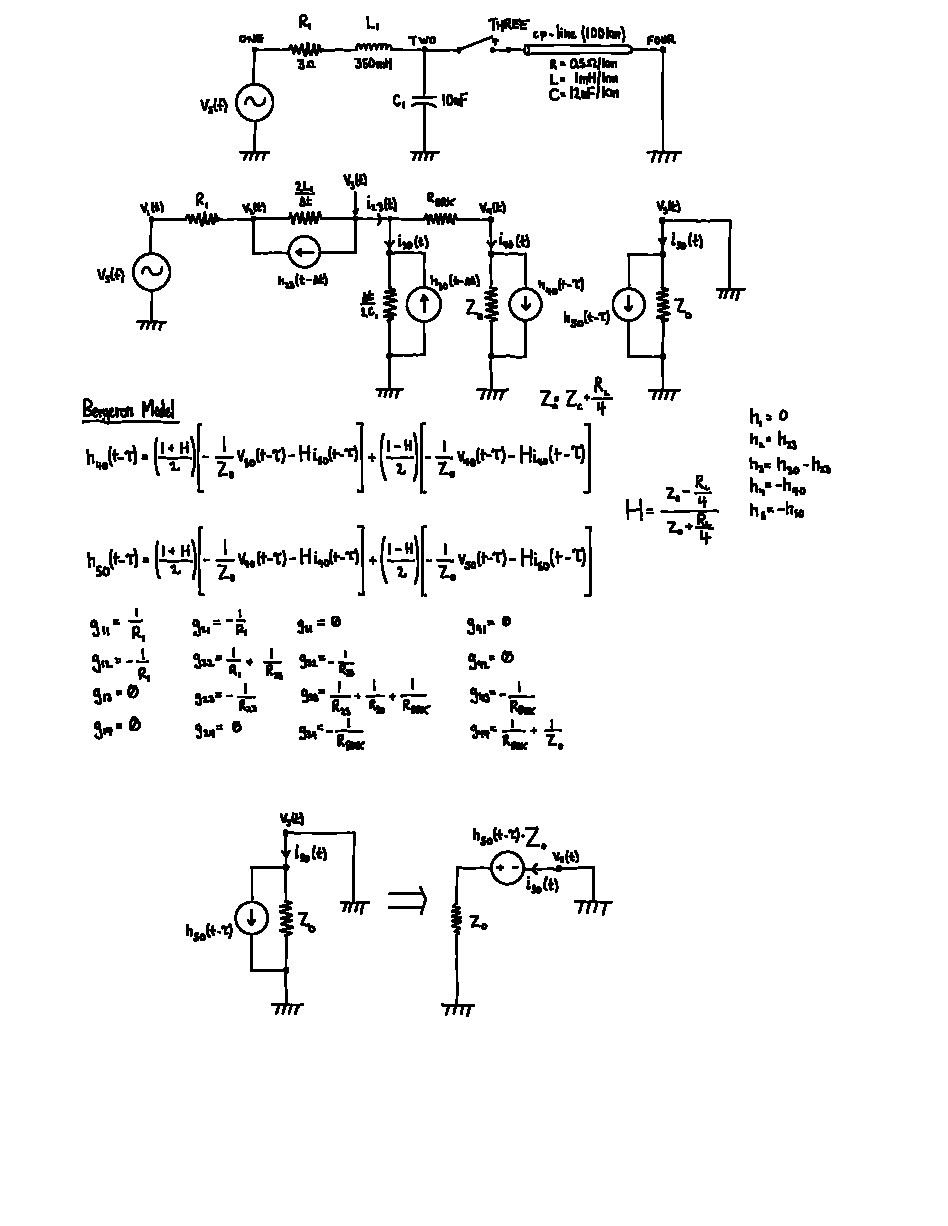
\includegraphics[width=5in]{schematic.png}
\caption{Transmission line's equivalent circuit and derivation of discretized components.}
\label{hand-setup}
\end{figure}

Once the current source histories are determined, the branch currents, which are required values for calculating the next nodal voltage values, can be calculated using the following relationships:

\begin{alignat}{2}
i_{23}(t) &= v_{23}(t)/R_{23} - h_{23}(t) \\
i_{30}(t) &= v_{30}(t)/R_{30} - h_{30}(t) \\
i_{40}(t) &= v_{40}(t)/R_{40} - h_{40}(t) \\
i_{50}(t) &= v_{50}(t)/R_{50} - h_{50}(t)
\end{alignat}

For this exercise, the convention used for currents leaving the node marks them as positive and currents entering the node marks them as negative. Therefore the resulting branch currents are the nodal voltage divided by the branch resistance, minus the discretized component current sources for all branch currents in this circuit.

Finally, we can now calculate the nodal voltage equations using some clever matrix manipulation taught in class. This technique subdivides the usual nodal analysis conductance matrix into four sections, with nodes connected to known voltage sources occupying the outside matrices $\mathbf{G_{AB}}$, $\mathbf{G_{BA}}$, and $\mathbf{G_{BB}}$. This allows us to perform the following operation to obtain our nodal voltage equation vector:

\begin{alignat}{2}
\left[\mathbf{V_A(t)}\right] &= \left[\mathbf{G_{AA}}\right]^{-1}\left[\mathbf{h_A(t)}\right] - \left[\mathbf{G_{AA}}\right]^{-1}\left[\mathbf{G_{AA}}\right]\left[\mathbf{V_B(t)}\right]
\end{alignat}

For this implementation, the breaker switch closing and opening has the effect of either connecting or breaking nodes 3 and 4 of the circuit (see Figure \ref{hand-setup} for node numbering). This has the result of generating two different conductance and history matrices. Shown below are both conductance and history matrices used for this circuit's solution:

\begin{alignat}{2}
  \left[
  \mathbf{G_{closed}}\right] &= \left[
      \begin{array}{c;{2pt/2pt}c}
        \mathbf{G_{AA}} & \mathbf{G_{AB}} \\ \hdashline[2pt/2pt]
        \mathbf{G_{BA}} & \mathbf{G_{BB}} 
      \end{array}
    \right] = \left[
      \begin{array}{ccc;{2pt/2pt}c}
        \frac{\Delta{}t}{2\,L_{1}}+\frac{1}{R_{1}} & -\frac{\Delta{}t}{2\,L_{1}} & 0 & -\frac{1}{R_{1}} \\ [6pt]
        -\frac{\Delta{}t}{2\,L_{1}} & \frac{2\,C_{1}}{\Delta{}t}+\frac{2\,C_{2}}{\Delta{}t}+\frac{\Delta{}t}{2\,L_{1}}+\frac{1}{R_{2}} & -\frac{1}{R_{2}} & 0 \\ [6pt]
        0 & -\frac{1}{R_{2}} & \frac{\Delta{}t}{2\,L_{2}}+\frac{1}{R_{2}} & 0 \\ [6pt] \hdashline[2pt/2pt]
        -\frac{1}{R_{1}} & 0 & 0 & \frac{1}{R_{1}}
      \end{array}
  \right] \\
  \left[
  \mathbf{G_{open}}\right] &= \left[
      \begin{array}{c;{2pt/2pt}c}
        \mathbf{G_{AA}} & \mathbf{G_{AB}} \\ \hdashline[2pt/2pt]
        \mathbf{G_{BA}} & \mathbf{G_{BB}} 
      \end{array}
    \right] = \left[\begin{array}{cccc;{2pt/2pt}c} \frac{\Delta{}t}{2\,L_{1}}+\frac{1}{R_{1}} & -\frac{\Delta{}t}{2\,L_{1}} & 0 & 0 & -\frac{1}{R_{1}} \\ [6pt]
    -\frac{\Delta{}t}{2\,L_{1}} & \frac{2\,C_{1}}{\Delta{}t}+\frac{\Delta{}t}{2\,L_{1}} & 0 & 0 & 0 \\ [6pt]
    0 & 0 & \frac{2\,C_{2}}{\Delta{}t}+\frac{1}{R_{2}} & -\frac{1}{R_{2}} & 0 \\ [6pt]
    0 & 0 & -\frac{1}{R_{2}} & \frac{\Delta{}t}{2\,L_{2}}+\frac{1}{R_{2}} & 0 \\ [6pt] \hdashline[2pt/2pt]
    -\frac{1}{R_{1}} & 0 & 0 & 0 & \frac{1}{R_{1}} \end{array}\right]
\end{alignat}

\begin{alignat}{2}
  \left[\mathbf{H_{closed}}\right] &= \left[\begin{array}{c} \mathbf{H_{A}} \\ \hdashline[2pt/2pt] \mathbf{H_{B}} \end{array}\right] = \left[\begin{array}{c} h_{23}(t) \\ -h_{23}(t) + h_{30}(t) + h_{40}(t) \\ h_{50}(t) \\ \hdashline[2pt/2pt] 0 \end{array}\right] \\
  \left[\mathbf{H_{open}}\right] &= \left[\begin{array}{c} \mathbf{H_{A}} \\ \hdashline[2pt/2pt] \mathbf{H_{B}} \end{array}\right] = \left[\begin{array}{c} h_{23}(t) \\ -h_{23}(t) + h_{30}(t) \\ h_{40}(t) \\ h_{50}(t) \\ \hdashline[2pt/2pt] 0 \end{array}\right]
\end{alignat}

The resulting nodal voltage equations were generated using MATLAB to minimize algebraic errors; the equations used to generate the nodal voltage equations were saved into a MATLAB file which can be viewed in Listing \ref{code-listing-matlab}. The resulting equations were then ported to a Python script which is provided in Listing \ref{code-listing-python}). There are two sets of nodal voltage solutions, one for the closed breaker and another for the open breaker. The closed breaker solution is used to begin with. Initial conditions are assumed to be zero for all variables. For each time step, the Python script then calculates the next nodal voltage value. These values are then used to calculate the next branch currents. After calculating the branch currents, the Python script checks if the breaker should have activated and if so, checks if the breaker current has changed sign since the last iteration. If both of these conditions are true, the breaker opens, effectively avoiding chopping current, and the open breaker solutions are used to calculate the nodal voltages until the end of the simulation. These results are plotted alongside the equivalent PSCAD solution for comparison using the Python matplotlib plotting library.

\subsection{Choosing a Simulation Time Step}

In order to choose an appropriate $\Delta{}t$ to simulate the circuit with, both sides of the circuit were analyzed for their resonant frequencies. This was performed by the following calculations:

\begin{alignat}{2}
f_{left} &= \frac{1}{2\pi\sqrt{L_1C_1}} = 2.69\,kHz \\
f_{right} &= \frac{1}{2\pi\sqrt{L_2C_2}} = 650\,Hz
\end{alignat}

The higher of the two frequencies, $2.69\,kHz$, corresponds to a period of $372\,\mu{}s$, so in order to get a good simulation result, an order of magnitude higher was chosen, at $\Delta{}t = 10\,\mu{}s$. 10 was chosen because it was a nice even number.

\subsection{PSCAD Simulation}

PSCAD provides a master library of components as well as primitives to help model the circuit. The resulting PSCAD circuit is shown in Figure \ref{pscad-setup}. The "Single Phase Voltage Source Model" component was used as the source and it was made ideal by setting the source impedance to $0 \Omega{}$ with a ramp-up time of $0 s$ (instantaneous voltage). The frequency was set to 60 Hz with a magnitude of $\frac{230}{\sqrt{2}}\,kV_{rms}$ and an offset of 90 degrees to match the assignment's voltage source equation of $230cos(377t)\,kV$. The ideal resistor, inductor, and capacitor were used to model the passive components and a series of voltmeters and ammeters were placed around the circuit to match the hand implemented solution. The voltage and current readings were piped to a plot on the same page as the schematic. In order to determine when PSCAD's breaker opened, the breaker's state variable was observed by plotting its value, and the resulting data is observed for a change that corresponds to an open state. The Python program plots both breaker opening times for the hand-implemented and PSCAD solutions (which turned out to be identical).

Once all of the components were hooked together and instrumented, the build button was clicked. This generated a Fortran program that models the entire circuit. A listing of this program can be found in Section \ref{code-listing-fortran}.

Clicking the run button ran the simulation and outputted the results on the plots. The data was extracted by right-clicking each plot{} to save it to the clipboard. This was then pasted into a CSV file for the Python program to read in as raw values.

\begin{figure}[H]
\centering
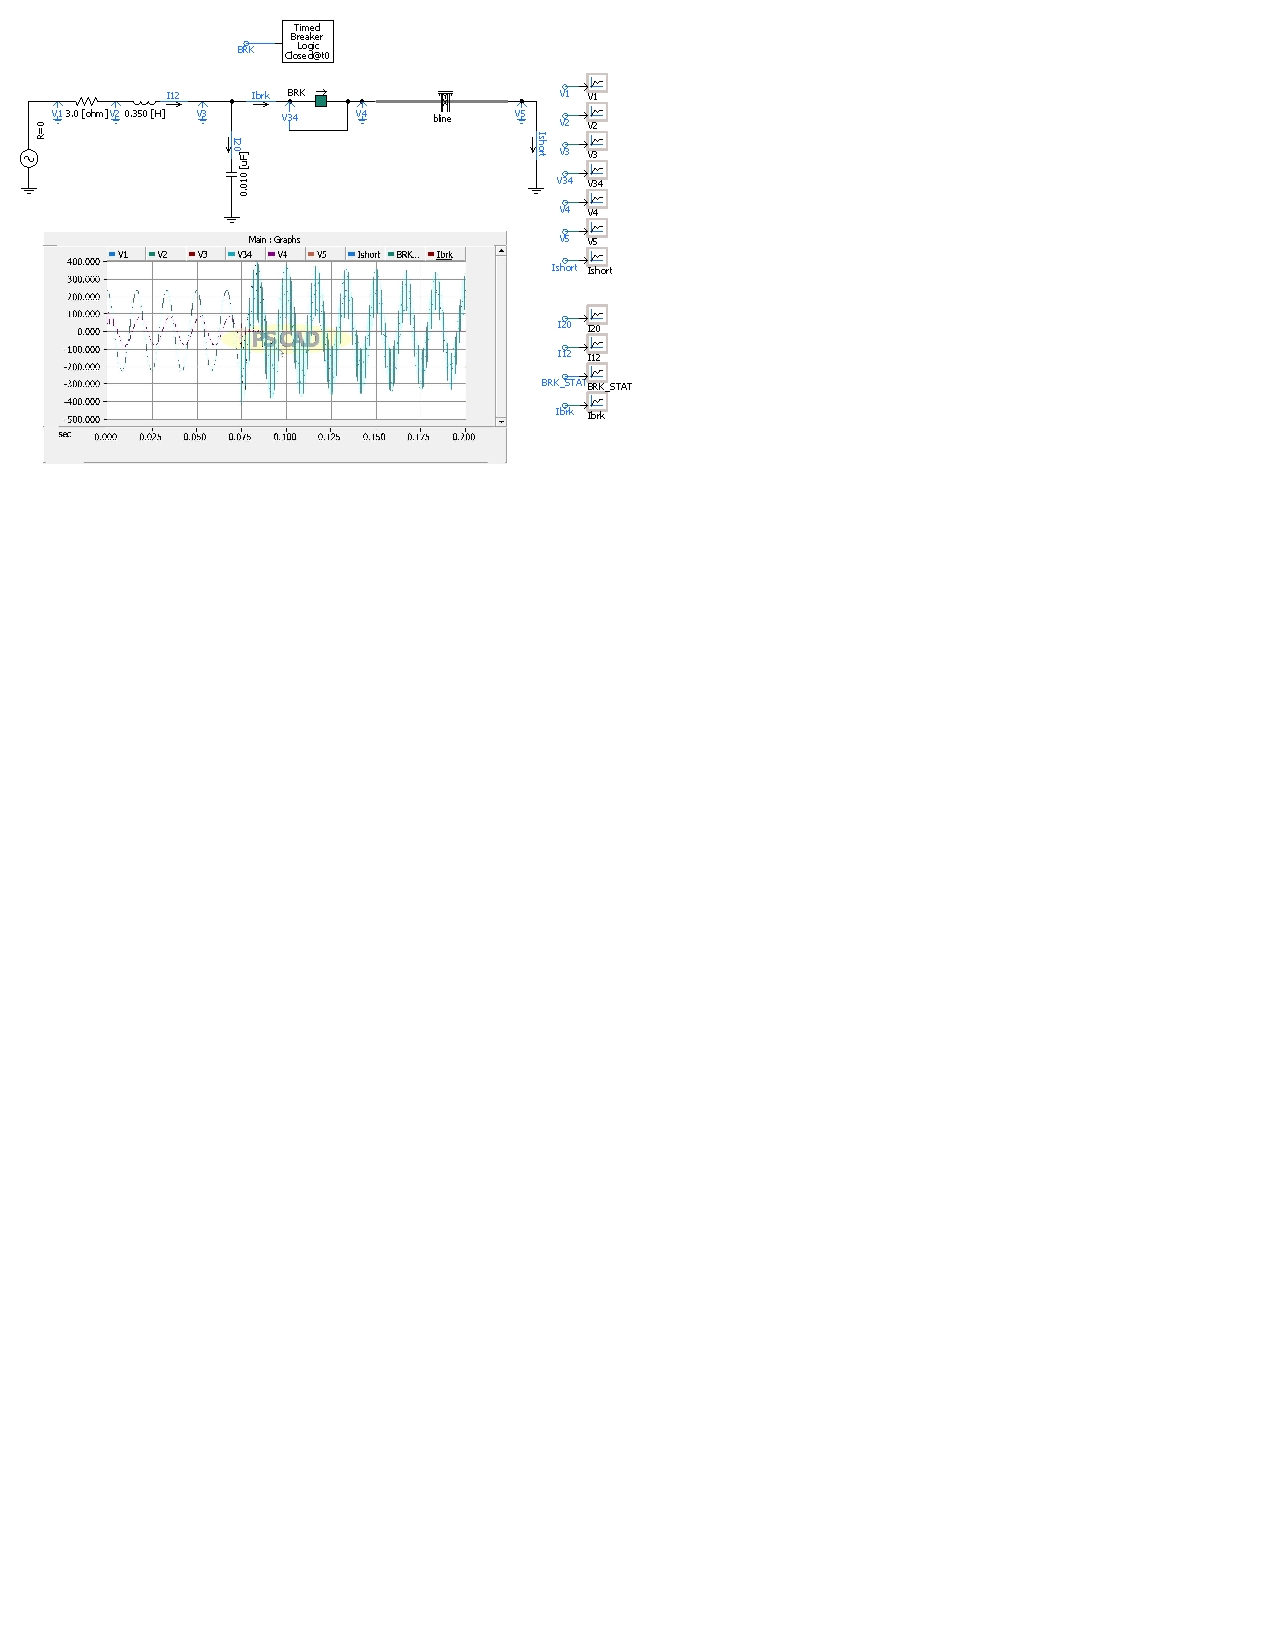
\includegraphics[width=5in]{pscad_schematic.png}
\caption{PSCAD schematic of transmission line.}
\label{pscad-setup}
\end{figure}

\section{Simulation}

With the hand-implemented and PSCAD solutions complete, the results can then be simulated and compared. This assignment requests the following comparison plots along with a zoomed-in portion for analysis. The figures following contain all of the plots required for the assignment.

\begin{enumerate}[label=\alph*)]
  \item Plots of $V_1$, $V_2$, $V_3$ for the simulation and PSCAD (Figures \ref{nodal_v_plots} and \ref{nodal_v_plots_zoom}).
  \item Plots of $I_{40}$ which represents the short-circuit current at the end of the transmission line (Figures \ref{short_circuit_i_plots} and \ref{short_circuit_i_plots_zoom}).
  \item Plots of $V_{23}$ which represents the voltage across the breaker (Figures \ref{breaker_v_plots} and \ref{breaker_v_plots_zoom}).
\end{enumerate}

Plots named simulation refer to the hand-modeled circuit and those named PSCAD refer to the PSCAD modeled circuit. In each plot, the red dashed line represents where the breaker has opened in the solution, which was identical between the hand-simulated and PSCAD solutions.

\begin{figure}[H]
    \begin{center}
        %% Creator: Matplotlib, PGF backend
%%
%% To include the figure in your LaTeX document, write
%%   \input{<filename>.pgf}
%%
%% Make sure the required packages are loaded in your preamble
%%   \usepackage{pgf}
%%
%% Figures using additional raster images can only be included by \input if
%% they are in the same directory as the main LaTeX file. For loading figures
%% from other directories you can use the `import` package
%%   \usepackage{import}
%% and then include the figures with
%%   \import{<path to file>}{<filename>.pgf}
%%
%% Matplotlib used the following preamble
%%
\begingroup%
\makeatletter%
\begin{pgfpicture}%
\pgfpathrectangle{\pgfpointorigin}{\pgfqpoint{6.500000in}{3.500000in}}%
\pgfusepath{use as bounding box}%
\begin{pgfscope}%
\pgfsetbuttcap%
\pgfsetroundjoin%
\definecolor{currentfill}{rgb}{1.000000,1.000000,1.000000}%
\pgfsetfillcolor{currentfill}%
\pgfsetlinewidth{0.000000pt}%
\definecolor{currentstroke}{rgb}{1.000000,1.000000,1.000000}%
\pgfsetstrokecolor{currentstroke}%
\pgfsetdash{}{0pt}%
\pgfpathmoveto{\pgfqpoint{0.000000in}{0.000000in}}%
\pgfpathlineto{\pgfqpoint{6.500000in}{0.000000in}}%
\pgfpathlineto{\pgfqpoint{6.500000in}{3.500000in}}%
\pgfpathlineto{\pgfqpoint{0.000000in}{3.500000in}}%
\pgfpathclose%
\pgfusepath{fill}%
\end{pgfscope}%
\begin{pgfscope}%
\pgfsetbuttcap%
\pgfsetroundjoin%
\definecolor{currentfill}{rgb}{1.000000,1.000000,1.000000}%
\pgfsetfillcolor{currentfill}%
\pgfsetlinewidth{0.000000pt}%
\definecolor{currentstroke}{rgb}{0.000000,0.000000,0.000000}%
\pgfsetstrokecolor{currentstroke}%
\pgfsetstrokeopacity{0.000000}%
\pgfsetdash{}{0pt}%
\pgfpathmoveto{\pgfqpoint{0.730248in}{0.537346in}}%
\pgfpathlineto{\pgfqpoint{6.157098in}{0.537346in}}%
\pgfpathlineto{\pgfqpoint{6.157098in}{3.164815in}}%
\pgfpathlineto{\pgfqpoint{0.730248in}{3.164815in}}%
\pgfpathclose%
\pgfusepath{fill}%
\end{pgfscope}%
\begin{pgfscope}%
\pgfpathrectangle{\pgfqpoint{0.730248in}{0.537346in}}{\pgfqpoint{5.426850in}{2.627470in}} %
\pgfusepath{clip}%
\pgfsetrectcap%
\pgfsetroundjoin%
\pgfsetlinewidth{1.003750pt}%
\definecolor{currentstroke}{rgb}{0.000000,0.000000,1.000000}%
\pgfsetstrokecolor{currentstroke}%
\pgfsetdash{}{0pt}%
\pgfpathmoveto{\pgfqpoint{0.730248in}{2.606478in}}%
\pgfpathlineto{\pgfqpoint{0.734047in}{2.605426in}}%
\pgfpathlineto{\pgfqpoint{0.738117in}{2.601968in}}%
\pgfpathlineto{\pgfqpoint{0.743001in}{2.594651in}}%
\pgfpathlineto{\pgfqpoint{0.748699in}{2.581791in}}%
\pgfpathlineto{\pgfqpoint{0.755483in}{2.560522in}}%
\pgfpathlineto{\pgfqpoint{0.763352in}{2.527976in}}%
\pgfpathlineto{\pgfqpoint{0.772577in}{2.479560in}}%
\pgfpathlineto{\pgfqpoint{0.783160in}{2.411381in}}%
\pgfpathlineto{\pgfqpoint{0.795641in}{2.315555in}}%
\pgfpathlineto{\pgfqpoint{0.810837in}{2.180405in}}%
\pgfpathlineto{\pgfqpoint{0.831187in}{1.977656in}}%
\pgfpathlineto{\pgfqpoint{0.881114in}{1.472254in}}%
\pgfpathlineto{\pgfqpoint{0.896852in}{1.339507in}}%
\pgfpathlineto{\pgfqpoint{0.909605in}{1.249548in}}%
\pgfpathlineto{\pgfqpoint{0.920459in}{1.187731in}}%
\pgfpathlineto{\pgfqpoint{0.929685in}{1.146978in}}%
\pgfpathlineto{\pgfqpoint{0.937554in}{1.121327in}}%
\pgfpathlineto{\pgfqpoint{0.944337in}{1.106200in}}%
\pgfpathlineto{\pgfqpoint{0.949764in}{1.098854in}}%
\pgfpathlineto{\pgfqpoint{0.954377in}{1.095970in}}%
\pgfpathlineto{\pgfqpoint{0.958447in}{1.096000in}}%
\pgfpathlineto{\pgfqpoint{0.962517in}{1.098444in}}%
\pgfpathlineto{\pgfqpoint{0.967130in}{1.104122in}}%
\pgfpathlineto{\pgfqpoint{0.972557in}{1.114726in}}%
\pgfpathlineto{\pgfqpoint{0.978798in}{1.132089in}}%
\pgfpathlineto{\pgfqpoint{0.986124in}{1.159353in}}%
\pgfpathlineto{\pgfqpoint{0.994807in}{1.200911in}}%
\pgfpathlineto{\pgfqpoint{1.004847in}{1.260698in}}%
\pgfpathlineto{\pgfqpoint{1.016514in}{1.344499in}}%
\pgfpathlineto{\pgfqpoint{1.030353in}{1.460911in}}%
\pgfpathlineto{\pgfqpoint{1.047990in}{1.629492in}}%
\pgfpathlineto{\pgfqpoint{1.080822in}{1.970274in}}%
\pgfpathlineto{\pgfqpoint{1.105243in}{2.211745in}}%
\pgfpathlineto{\pgfqpoint{1.121252in}{2.349281in}}%
\pgfpathlineto{\pgfqpoint{1.134277in}{2.443339in}}%
\pgfpathlineto{\pgfqpoint{1.145402in}{2.508466in}}%
\pgfpathlineto{\pgfqpoint{1.154899in}{2.551709in}}%
\pgfpathlineto{\pgfqpoint{1.163039in}{2.579103in}}%
\pgfpathlineto{\pgfqpoint{1.169823in}{2.594837in}}%
\pgfpathlineto{\pgfqpoint{1.175521in}{2.602955in}}%
\pgfpathlineto{\pgfqpoint{1.180134in}{2.606078in}}%
\pgfpathlineto{\pgfqpoint{1.184204in}{2.606260in}}%
\pgfpathlineto{\pgfqpoint{1.188274in}{2.604027in}}%
\pgfpathlineto{\pgfqpoint{1.192887in}{2.598587in}}%
\pgfpathlineto{\pgfqpoint{1.198314in}{2.588260in}}%
\pgfpathlineto{\pgfqpoint{1.204555in}{2.571210in}}%
\pgfpathlineto{\pgfqpoint{1.211881in}{2.544303in}}%
\pgfpathlineto{\pgfqpoint{1.220292in}{2.504579in}}%
\pgfpathlineto{\pgfqpoint{1.230061in}{2.447303in}}%
\pgfpathlineto{\pgfqpoint{1.241457in}{2.366708in}}%
\pgfpathlineto{\pgfqpoint{1.255024in}{2.254129in}}%
\pgfpathlineto{\pgfqpoint{1.272119in}{2.092494in}}%
\pgfpathlineto{\pgfqpoint{1.300339in}{1.800666in}}%
\pgfpathlineto{\pgfqpoint{1.328830in}{1.513938in}}%
\pgfpathlineto{\pgfqpoint{1.345653in}{1.366536in}}%
\pgfpathlineto{\pgfqpoint{1.358949in}{1.268333in}}%
\pgfpathlineto{\pgfqpoint{1.370345in}{1.199833in}}%
\pgfpathlineto{\pgfqpoint{1.380113in}{1.154034in}}%
\pgfpathlineto{\pgfqpoint{1.388254in}{1.125632in}}%
\pgfpathlineto{\pgfqpoint{1.395308in}{1.108504in}}%
\pgfpathlineto{\pgfqpoint{1.401007in}{1.099870in}}%
\pgfpathlineto{\pgfqpoint{1.405891in}{1.096213in}}%
\pgfpathlineto{\pgfqpoint{1.409961in}{1.095820in}}%
\pgfpathlineto{\pgfqpoint{1.414031in}{1.097842in}}%
\pgfpathlineto{\pgfqpoint{1.418373in}{1.102652in}}%
\pgfpathlineto{\pgfqpoint{1.423528in}{1.111898in}}%
\pgfpathlineto{\pgfqpoint{1.429769in}{1.128157in}}%
\pgfpathlineto{\pgfqpoint{1.437095in}{1.154163in}}%
\pgfpathlineto{\pgfqpoint{1.445507in}{1.192899in}}%
\pgfpathlineto{\pgfqpoint{1.455275in}{1.249110in}}%
\pgfpathlineto{\pgfqpoint{1.466671in}{1.328597in}}%
\pgfpathlineto{\pgfqpoint{1.480239in}{1.440082in}}%
\pgfpathlineto{\pgfqpoint{1.497062in}{1.598058in}}%
\pgfpathlineto{\pgfqpoint{1.523653in}{1.872158in}}%
\pgfpathlineto{\pgfqpoint{1.554315in}{2.182313in}}%
\pgfpathlineto{\pgfqpoint{1.571138in}{2.330552in}}%
\pgfpathlineto{\pgfqpoint{1.584705in}{2.431440in}}%
\pgfpathlineto{\pgfqpoint{1.596102in}{2.500424in}}%
\pgfpathlineto{\pgfqpoint{1.605870in}{2.546677in}}%
\pgfpathlineto{\pgfqpoint{1.614010in}{2.575477in}}%
\pgfpathlineto{\pgfqpoint{1.621065in}{2.592961in}}%
\pgfpathlineto{\pgfqpoint{1.626764in}{2.601888in}}%
\pgfpathlineto{\pgfqpoint{1.631648in}{2.605798in}}%
\pgfpathlineto{\pgfqpoint{1.635718in}{2.606403in}}%
\pgfpathlineto{\pgfqpoint{1.639788in}{2.604592in}}%
\pgfpathlineto{\pgfqpoint{1.644130in}{2.600006in}}%
\pgfpathlineto{\pgfqpoint{1.649285in}{2.591025in}}%
\pgfpathlineto{\pgfqpoint{1.655255in}{2.575887in}}%
\pgfpathlineto{\pgfqpoint{1.662309in}{2.551584in}}%
\pgfpathlineto{\pgfqpoint{1.670450in}{2.515203in}}%
\pgfpathlineto{\pgfqpoint{1.679947in}{2.462072in}}%
\pgfpathlineto{\pgfqpoint{1.691072in}{2.386400in}}%
\pgfpathlineto{\pgfqpoint{1.704096in}{2.281738in}}%
\pgfpathlineto{\pgfqpoint{1.720377in}{2.131579in}}%
\pgfpathlineto{\pgfqpoint{1.744255in}{1.887836in}}%
\pgfpathlineto{\pgfqpoint{1.780615in}{1.518092in}}%
\pgfpathlineto{\pgfqpoint{1.797438in}{1.370100in}}%
\pgfpathlineto{\pgfqpoint{1.811005in}{1.269472in}}%
\pgfpathlineto{\pgfqpoint{1.822402in}{1.200741in}}%
\pgfpathlineto{\pgfqpoint{1.832170in}{1.154724in}}%
\pgfpathlineto{\pgfqpoint{1.840310in}{1.126132in}}%
\pgfpathlineto{\pgfqpoint{1.847365in}{1.108834in}}%
\pgfpathlineto{\pgfqpoint{1.853063in}{1.100060in}}%
\pgfpathlineto{\pgfqpoint{1.857947in}{1.096282in}}%
\pgfpathlineto{\pgfqpoint{1.862018in}{1.095788in}}%
\pgfpathlineto{\pgfqpoint{1.866088in}{1.097709in}}%
\pgfpathlineto{\pgfqpoint{1.870429in}{1.102412in}}%
\pgfpathlineto{\pgfqpoint{1.875585in}{1.111532in}}%
\pgfpathlineto{\pgfqpoint{1.881826in}{1.127641in}}%
\pgfpathlineto{\pgfqpoint{1.888880in}{1.152388in}}%
\pgfpathlineto{\pgfqpoint{1.897292in}{1.190637in}}%
\pgfpathlineto{\pgfqpoint{1.907060in}{1.246321in}}%
\pgfpathlineto{\pgfqpoint{1.918457in}{1.325260in}}%
\pgfpathlineto{\pgfqpoint{1.931753in}{1.433825in}}%
\pgfpathlineto{\pgfqpoint{1.948304in}{1.588349in}}%
\pgfpathlineto{\pgfqpoint{1.973811in}{1.850439in}}%
\pgfpathlineto{\pgfqpoint{2.006372in}{2.180706in}}%
\pgfpathlineto{\pgfqpoint{2.023195in}{2.329170in}}%
\pgfpathlineto{\pgfqpoint{2.036762in}{2.430295in}}%
\pgfpathlineto{\pgfqpoint{2.048159in}{2.499509in}}%
\pgfpathlineto{\pgfqpoint{2.057927in}{2.545978in}}%
\pgfpathlineto{\pgfqpoint{2.066338in}{2.575777in}}%
\pgfpathlineto{\pgfqpoint{2.073393in}{2.593160in}}%
\pgfpathlineto{\pgfqpoint{2.079092in}{2.602004in}}%
\pgfpathlineto{\pgfqpoint{2.083976in}{2.605842in}}%
\pgfpathlineto{\pgfqpoint{2.088046in}{2.606387in}}%
\pgfpathlineto{\pgfqpoint{2.092116in}{2.604517in}}%
\pgfpathlineto{\pgfqpoint{2.096457in}{2.599867in}}%
\pgfpathlineto{\pgfqpoint{2.101613in}{2.590810in}}%
\pgfpathlineto{\pgfqpoint{2.107583in}{2.575588in}}%
\pgfpathlineto{\pgfqpoint{2.114637in}{2.551186in}}%
\pgfpathlineto{\pgfqpoint{2.122778in}{2.514697in}}%
\pgfpathlineto{\pgfqpoint{2.132275in}{2.461447in}}%
\pgfpathlineto{\pgfqpoint{2.143400in}{2.385651in}}%
\pgfpathlineto{\pgfqpoint{2.156424in}{2.280866in}}%
\pgfpathlineto{\pgfqpoint{2.172705in}{2.130594in}}%
\pgfpathlineto{\pgfqpoint{2.196583in}{1.886776in}}%
\pgfpathlineto{\pgfqpoint{2.232943in}{1.517140in}}%
\pgfpathlineto{\pgfqpoint{2.249766in}{1.369282in}}%
\pgfpathlineto{\pgfqpoint{2.263333in}{1.268795in}}%
\pgfpathlineto{\pgfqpoint{2.274730in}{1.200201in}}%
\pgfpathlineto{\pgfqpoint{2.284498in}{1.154314in}}%
\pgfpathlineto{\pgfqpoint{2.292638in}{1.125834in}}%
\pgfpathlineto{\pgfqpoint{2.299693in}{1.108638in}}%
\pgfpathlineto{\pgfqpoint{2.305391in}{1.099947in}}%
\pgfpathlineto{\pgfqpoint{2.310275in}{1.096241in}}%
\pgfpathlineto{\pgfqpoint{2.314346in}{1.095807in}}%
\pgfpathlineto{\pgfqpoint{2.318416in}{1.097787in}}%
\pgfpathlineto{\pgfqpoint{2.322757in}{1.102554in}}%
\pgfpathlineto{\pgfqpoint{2.327913in}{1.111749in}}%
\pgfpathlineto{\pgfqpoint{2.334154in}{1.127947in}}%
\pgfpathlineto{\pgfqpoint{2.341480in}{1.153883in}}%
\pgfpathlineto{\pgfqpoint{2.349891in}{1.192543in}}%
\pgfpathlineto{\pgfqpoint{2.359660in}{1.248671in}}%
\pgfpathlineto{\pgfqpoint{2.371056in}{1.328073in}}%
\pgfpathlineto{\pgfqpoint{2.384623in}{1.439474in}}%
\pgfpathlineto{\pgfqpoint{2.401446in}{1.597375in}}%
\pgfpathlineto{\pgfqpoint{2.428038in}{1.871432in}}%
\pgfpathlineto{\pgfqpoint{2.458700in}{2.181661in}}%
\pgfpathlineto{\pgfqpoint{2.475523in}{2.329991in}}%
\pgfpathlineto{\pgfqpoint{2.489090in}{2.430975in}}%
\pgfpathlineto{\pgfqpoint{2.500486in}{2.500053in}}%
\pgfpathlineto{\pgfqpoint{2.510255in}{2.546393in}}%
\pgfpathlineto{\pgfqpoint{2.518666in}{2.576076in}}%
\pgfpathlineto{\pgfqpoint{2.525721in}{2.593357in}}%
\pgfpathlineto{\pgfqpoint{2.531420in}{2.602119in}}%
\pgfpathlineto{\pgfqpoint{2.536304in}{2.605885in}}%
\pgfpathlineto{\pgfqpoint{2.540374in}{2.606370in}}%
\pgfpathlineto{\pgfqpoint{2.544444in}{2.604440in}}%
\pgfpathlineto{\pgfqpoint{2.548785in}{2.599726in}}%
\pgfpathlineto{\pgfqpoint{2.553941in}{2.590595in}}%
\pgfpathlineto{\pgfqpoint{2.560182in}{2.574472in}}%
\pgfpathlineto{\pgfqpoint{2.567237in}{2.549709in}}%
\pgfpathlineto{\pgfqpoint{2.575648in}{2.511442in}}%
\pgfpathlineto{\pgfqpoint{2.585417in}{2.455739in}}%
\pgfpathlineto{\pgfqpoint{2.596813in}{2.376781in}}%
\pgfpathlineto{\pgfqpoint{2.610109in}{2.268196in}}%
\pgfpathlineto{\pgfqpoint{2.626661in}{2.113655in}}%
\pgfpathlineto{\pgfqpoint{2.652167in}{1.851554in}}%
\pgfpathlineto{\pgfqpoint{2.684728in}{1.521303in}}%
\pgfpathlineto{\pgfqpoint{2.701551in}{1.372861in}}%
\pgfpathlineto{\pgfqpoint{2.715118in}{1.271758in}}%
\pgfpathlineto{\pgfqpoint{2.726515in}{1.202566in}}%
\pgfpathlineto{\pgfqpoint{2.736283in}{1.156117in}}%
\pgfpathlineto{\pgfqpoint{2.744695in}{1.126336in}}%
\pgfpathlineto{\pgfqpoint{2.751750in}{1.108970in}}%
\pgfpathlineto{\pgfqpoint{2.757448in}{1.100138in}}%
\pgfpathlineto{\pgfqpoint{2.762332in}{1.096312in}}%
\pgfpathlineto{\pgfqpoint{2.766402in}{1.095776in}}%
\pgfpathlineto{\pgfqpoint{2.770472in}{1.097656in}}%
\pgfpathlineto{\pgfqpoint{2.774814in}{1.102316in}}%
\pgfpathlineto{\pgfqpoint{2.779969in}{1.111384in}}%
\pgfpathlineto{\pgfqpoint{2.785939in}{1.126620in}}%
\pgfpathlineto{\pgfqpoint{2.792994in}{1.151038in}}%
\pgfpathlineto{\pgfqpoint{2.801134in}{1.187544in}}%
\pgfpathlineto{\pgfqpoint{2.810631in}{1.240812in}}%
\pgfpathlineto{\pgfqpoint{2.821756in}{1.316628in}}%
\pgfpathlineto{\pgfqpoint{2.834780in}{1.421433in}}%
\pgfpathlineto{\pgfqpoint{2.851061in}{1.571723in}}%
\pgfpathlineto{\pgfqpoint{2.874939in}{1.815552in}}%
\pgfpathlineto{\pgfqpoint{2.911299in}{2.185171in}}%
\pgfpathlineto{\pgfqpoint{2.928122in}{2.333007in}}%
\pgfpathlineto{\pgfqpoint{2.941689in}{2.433473in}}%
\pgfpathlineto{\pgfqpoint{2.953086in}{2.502044in}}%
\pgfpathlineto{\pgfqpoint{2.962854in}{2.547912in}}%
\pgfpathlineto{\pgfqpoint{2.970994in}{2.576373in}}%
\pgfpathlineto{\pgfqpoint{2.978049in}{2.593554in}}%
\pgfpathlineto{\pgfqpoint{2.983747in}{2.602232in}}%
\pgfpathlineto{\pgfqpoint{2.988632in}{2.605926in}}%
\pgfpathlineto{\pgfqpoint{2.992702in}{2.606351in}}%
\pgfpathlineto{\pgfqpoint{2.996772in}{2.604361in}}%
\pgfpathlineto{\pgfqpoint{3.001113in}{2.599584in}}%
\pgfpathlineto{\pgfqpoint{3.006269in}{2.590377in}}%
\pgfpathlineto{\pgfqpoint{3.012510in}{2.574165in}}%
\pgfpathlineto{\pgfqpoint{3.019836in}{2.548213in}}%
\pgfpathlineto{\pgfqpoint{3.028248in}{2.509535in}}%
\pgfpathlineto{\pgfqpoint{3.038016in}{2.453388in}}%
\pgfpathlineto{\pgfqpoint{3.049412in}{2.373966in}}%
\pgfpathlineto{\pgfqpoint{3.062980in}{2.262546in}}%
\pgfpathlineto{\pgfqpoint{3.079803in}{2.104628in}}%
\pgfpathlineto{\pgfqpoint{3.106394in}{1.830561in}}%
\pgfpathlineto{\pgfqpoint{3.137056in}{1.520349in}}%
\pgfpathlineto{\pgfqpoint{3.153879in}{1.372040in}}%
\pgfpathlineto{\pgfqpoint{3.167446in}{1.271078in}}%
\pgfpathlineto{\pgfqpoint{3.178843in}{1.202022in}}%
\pgfpathlineto{\pgfqpoint{3.188611in}{1.155702in}}%
\pgfpathlineto{\pgfqpoint{3.197023in}{1.126037in}}%
\pgfpathlineto{\pgfqpoint{3.204078in}{1.108772in}}%
\pgfpathlineto{\pgfqpoint{3.209776in}{1.100024in}}%
\pgfpathlineto{\pgfqpoint{3.214660in}{1.096269in}}%
\pgfpathlineto{\pgfqpoint{3.218730in}{1.095794in}}%
\pgfpathlineto{\pgfqpoint{3.222800in}{1.097734in}}%
\pgfpathlineto{\pgfqpoint{3.227142in}{1.102457in}}%
\pgfpathlineto{\pgfqpoint{3.232297in}{1.111600in}}%
\pgfpathlineto{\pgfqpoint{3.238538in}{1.127737in}}%
\pgfpathlineto{\pgfqpoint{3.245593in}{1.152516in}}%
\pgfpathlineto{\pgfqpoint{3.254005in}{1.190800in}}%
\pgfpathlineto{\pgfqpoint{3.263773in}{1.246522in}}%
\pgfpathlineto{\pgfqpoint{3.275169in}{1.325501in}}%
\pgfpathlineto{\pgfqpoint{3.288465in}{1.434104in}}%
\pgfpathlineto{\pgfqpoint{3.305017in}{1.588663in}}%
\pgfpathlineto{\pgfqpoint{3.330523in}{1.850774in}}%
\pgfpathlineto{\pgfqpoint{3.363084in}{2.181008in}}%
\pgfpathlineto{\pgfqpoint{3.379908in}{2.329430in}}%
\pgfpathlineto{\pgfqpoint{3.393475in}{2.430510in}}%
\pgfpathlineto{\pgfqpoint{3.404871in}{2.499681in}}%
\pgfpathlineto{\pgfqpoint{3.414639in}{2.546109in}}%
\pgfpathlineto{\pgfqpoint{3.423051in}{2.575872in}}%
\pgfpathlineto{\pgfqpoint{3.430106in}{2.593222in}}%
\pgfpathlineto{\pgfqpoint{3.435804in}{2.602041in}}%
\pgfpathlineto{\pgfqpoint{3.440688in}{2.605856in}}%
\pgfpathlineto{\pgfqpoint{3.444758in}{2.606382in}}%
\pgfpathlineto{\pgfqpoint{3.448829in}{2.604492in}}%
\pgfpathlineto{\pgfqpoint{3.453170in}{2.599823in}}%
\pgfpathlineto{\pgfqpoint{3.458326in}{2.590742in}}%
\pgfpathlineto{\pgfqpoint{3.464295in}{2.575493in}}%
\pgfpathlineto{\pgfqpoint{3.471350in}{2.551060in}}%
\pgfpathlineto{\pgfqpoint{3.479490in}{2.514536in}}%
\pgfpathlineto{\pgfqpoint{3.488987in}{2.461249in}}%
\pgfpathlineto{\pgfqpoint{3.500112in}{2.385414in}}%
\pgfpathlineto{\pgfqpoint{3.513137in}{2.280590in}}%
\pgfpathlineto{\pgfqpoint{3.529417in}{2.130282in}}%
\pgfpathlineto{\pgfqpoint{3.553295in}{1.886441in}}%
\pgfpathlineto{\pgfqpoint{3.589655in}{1.516839in}}%
\pgfpathlineto{\pgfqpoint{3.606479in}{1.369024in}}%
\pgfpathlineto{\pgfqpoint{3.620046in}{1.268581in}}%
\pgfpathlineto{\pgfqpoint{3.631442in}{1.200031in}}%
\pgfpathlineto{\pgfqpoint{3.641210in}{1.154184in}}%
\pgfpathlineto{\pgfqpoint{3.649351in}{1.125740in}}%
\pgfpathlineto{\pgfqpoint{3.656406in}{1.108576in}}%
\pgfpathlineto{\pgfqpoint{3.662104in}{1.099911in}}%
\pgfpathlineto{\pgfqpoint{3.666988in}{1.096228in}}%
\pgfpathlineto{\pgfqpoint{3.671058in}{1.095813in}}%
\pgfpathlineto{\pgfqpoint{3.675128in}{1.097812in}}%
\pgfpathlineto{\pgfqpoint{3.679470in}{1.102599in}}%
\pgfpathlineto{\pgfqpoint{3.684625in}{1.111818in}}%
\pgfpathlineto{\pgfqpoint{3.690866in}{1.128044in}}%
\pgfpathlineto{\pgfqpoint{3.698192in}{1.154013in}}%
\pgfpathlineto{\pgfqpoint{3.706604in}{1.192708in}}%
\pgfpathlineto{\pgfqpoint{3.716372in}{1.248874in}}%
\pgfpathlineto{\pgfqpoint{3.727769in}{1.328315in}}%
\pgfpathlineto{\pgfqpoint{3.741336in}{1.439755in}}%
\pgfpathlineto{\pgfqpoint{3.758159in}{1.597691in}}%
\pgfpathlineto{\pgfqpoint{3.784751in}{1.871767in}}%
\pgfpathlineto{\pgfqpoint{3.815412in}{2.181962in}}%
\pgfpathlineto{\pgfqpoint{3.832236in}{2.330250in}}%
\pgfpathlineto{\pgfqpoint{3.845803in}{2.431190in}}%
\pgfpathlineto{\pgfqpoint{3.857199in}{2.500224in}}%
\pgfpathlineto{\pgfqpoint{3.866967in}{2.546524in}}%
\pgfpathlineto{\pgfqpoint{3.875108in}{2.575367in}}%
\pgfpathlineto{\pgfqpoint{3.882163in}{2.592887in}}%
\pgfpathlineto{\pgfqpoint{3.887861in}{2.601845in}}%
\pgfpathlineto{\pgfqpoint{3.892745in}{2.605781in}}%
\pgfpathlineto{\pgfqpoint{3.896815in}{2.606408in}}%
\pgfpathlineto{\pgfqpoint{3.900614in}{2.604814in}}%
\pgfpathlineto{\pgfqpoint{3.904955in}{2.600423in}}%
\pgfpathlineto{\pgfqpoint{3.910111in}{2.591669in}}%
\pgfpathlineto{\pgfqpoint{3.916080in}{2.576793in}}%
\pgfpathlineto{\pgfqpoint{3.923135in}{2.552789in}}%
\pgfpathlineto{\pgfqpoint{3.931276in}{2.516740in}}%
\pgfpathlineto{\pgfqpoint{3.940773in}{2.463970in}}%
\pgfpathlineto{\pgfqpoint{3.951898in}{2.388680in}}%
\pgfpathlineto{\pgfqpoint{3.964922in}{2.284395in}}%
\pgfpathlineto{\pgfqpoint{3.980931in}{2.137221in}}%
\pgfpathlineto{\pgfqpoint{4.004267in}{1.899599in}}%
\pgfpathlineto{\pgfqpoint{4.042255in}{1.513338in}}%
\pgfpathlineto{\pgfqpoint{4.059078in}{1.366021in}}%
\pgfpathlineto{\pgfqpoint{4.072374in}{1.267906in}}%
\pgfpathlineto{\pgfqpoint{4.083770in}{1.199494in}}%
\pgfpathlineto{\pgfqpoint{4.093538in}{1.153775in}}%
\pgfpathlineto{\pgfqpoint{4.101679in}{1.125445in}}%
\pgfpathlineto{\pgfqpoint{4.108734in}{1.108382in}}%
\pgfpathlineto{\pgfqpoint{4.114432in}{1.099800in}}%
\pgfpathlineto{\pgfqpoint{4.119045in}{1.096298in}}%
\pgfpathlineto{\pgfqpoint{4.123115in}{1.095782in}}%
\pgfpathlineto{\pgfqpoint{4.127185in}{1.097680in}}%
\pgfpathlineto{\pgfqpoint{4.131526in}{1.102360in}}%
\pgfpathlineto{\pgfqpoint{4.136682in}{1.111453in}}%
\pgfpathlineto{\pgfqpoint{4.142651in}{1.126715in}}%
\pgfpathlineto{\pgfqpoint{4.149706in}{1.151164in}}%
\pgfpathlineto{\pgfqpoint{4.158118in}{1.189071in}}%
\pgfpathlineto{\pgfqpoint{4.167615in}{1.242694in}}%
\pgfpathlineto{\pgfqpoint{4.178740in}{1.318883in}}%
\pgfpathlineto{\pgfqpoint{4.192036in}{1.426407in}}%
\pgfpathlineto{\pgfqpoint{4.208316in}{1.577335in}}%
\pgfpathlineto{\pgfqpoint{4.232737in}{1.827270in}}%
\pgfpathlineto{\pgfqpoint{4.267740in}{2.182916in}}%
\pgfpathlineto{\pgfqpoint{4.284564in}{2.331070in}}%
\pgfpathlineto{\pgfqpoint{4.298131in}{2.431869in}}%
\pgfpathlineto{\pgfqpoint{4.309527in}{2.500766in}}%
\pgfpathlineto{\pgfqpoint{4.319295in}{2.546938in}}%
\pgfpathlineto{\pgfqpoint{4.327436in}{2.575667in}}%
\pgfpathlineto{\pgfqpoint{4.334491in}{2.593087in}}%
\pgfpathlineto{\pgfqpoint{4.340189in}{2.601962in}}%
\pgfpathlineto{\pgfqpoint{4.345073in}{2.605826in}}%
\pgfpathlineto{\pgfqpoint{4.349143in}{2.606393in}}%
\pgfpathlineto{\pgfqpoint{4.353213in}{2.604545in}}%
\pgfpathlineto{\pgfqpoint{4.357555in}{2.599919in}}%
\pgfpathlineto{\pgfqpoint{4.362710in}{2.590889in}}%
\pgfpathlineto{\pgfqpoint{4.368680in}{2.575698in}}%
\pgfpathlineto{\pgfqpoint{4.375735in}{2.551333in}}%
\pgfpathlineto{\pgfqpoint{4.383875in}{2.514883in}}%
\pgfpathlineto{\pgfqpoint{4.393372in}{2.461677in}}%
\pgfpathlineto{\pgfqpoint{4.404497in}{2.385927in}}%
\pgfpathlineto{\pgfqpoint{4.417521in}{2.281187in}}%
\pgfpathlineto{\pgfqpoint{4.433802in}{2.130956in}}%
\pgfpathlineto{\pgfqpoint{4.457680in}{1.887166in}}%
\pgfpathlineto{\pgfqpoint{4.494040in}{1.517490in}}%
\pgfpathlineto{\pgfqpoint{4.510863in}{1.369583in}}%
\pgfpathlineto{\pgfqpoint{4.524430in}{1.269044in}}%
\pgfpathlineto{\pgfqpoint{4.535827in}{1.200399in}}%
\pgfpathlineto{\pgfqpoint{4.545595in}{1.154465in}}%
\pgfpathlineto{\pgfqpoint{4.553735in}{1.125943in}}%
\pgfpathlineto{\pgfqpoint{4.560790in}{1.108710in}}%
\pgfpathlineto{\pgfqpoint{4.566488in}{1.099988in}}%
\pgfpathlineto{\pgfqpoint{4.571373in}{1.096256in}}%
\pgfpathlineto{\pgfqpoint{4.575443in}{1.095800in}}%
\pgfpathlineto{\pgfqpoint{4.579513in}{1.097758in}}%
\pgfpathlineto{\pgfqpoint{4.583854in}{1.102502in}}%
\pgfpathlineto{\pgfqpoint{4.589010in}{1.111669in}}%
\pgfpathlineto{\pgfqpoint{4.595251in}{1.127834in}}%
\pgfpathlineto{\pgfqpoint{4.602306in}{1.152643in}}%
\pgfpathlineto{\pgfqpoint{4.610717in}{1.190963in}}%
\pgfpathlineto{\pgfqpoint{4.620486in}{1.246723in}}%
\pgfpathlineto{\pgfqpoint{4.631882in}{1.325742in}}%
\pgfpathlineto{\pgfqpoint{4.645178in}{1.434384in}}%
\pgfpathlineto{\pgfqpoint{4.661730in}{1.588978in}}%
\pgfpathlineto{\pgfqpoint{4.687236in}{1.851109in}}%
\pgfpathlineto{\pgfqpoint{4.719797in}{2.181310in}}%
\pgfpathlineto{\pgfqpoint{4.736620in}{2.329689in}}%
\pgfpathlineto{\pgfqpoint{4.750187in}{2.430725in}}%
\pgfpathlineto{\pgfqpoint{4.761584in}{2.499853in}}%
\pgfpathlineto{\pgfqpoint{4.771352in}{2.546241in}}%
\pgfpathlineto{\pgfqpoint{4.779764in}{2.575966in}}%
\pgfpathlineto{\pgfqpoint{4.786818in}{2.593285in}}%
\pgfpathlineto{\pgfqpoint{4.792517in}{2.602077in}}%
\pgfpathlineto{\pgfqpoint{4.797401in}{2.605869in}}%
\pgfpathlineto{\pgfqpoint{4.801471in}{2.606376in}}%
\pgfpathlineto{\pgfqpoint{4.805541in}{2.604468in}}%
\pgfpathlineto{\pgfqpoint{4.809883in}{2.599778in}}%
\pgfpathlineto{\pgfqpoint{4.815038in}{2.590674in}}%
\pgfpathlineto{\pgfqpoint{4.821008in}{2.575398in}}%
\pgfpathlineto{\pgfqpoint{4.828063in}{2.550934in}}%
\pgfpathlineto{\pgfqpoint{4.836474in}{2.513008in}}%
\pgfpathlineto{\pgfqpoint{4.845971in}{2.459367in}}%
\pgfpathlineto{\pgfqpoint{4.857096in}{2.383159in}}%
\pgfpathlineto{\pgfqpoint{4.870392in}{2.275615in}}%
\pgfpathlineto{\pgfqpoint{4.886673in}{2.124669in}}%
\pgfpathlineto{\pgfqpoint{4.911093in}{1.874724in}}%
\pgfpathlineto{\pgfqpoint{4.946097in}{1.519094in}}%
\pgfpathlineto{\pgfqpoint{4.962920in}{1.370961in}}%
\pgfpathlineto{\pgfqpoint{4.976487in}{1.270184in}}%
\pgfpathlineto{\pgfqpoint{4.987883in}{1.201309in}}%
\pgfpathlineto{\pgfqpoint{4.997652in}{1.155157in}}%
\pgfpathlineto{\pgfqpoint{5.005792in}{1.126446in}}%
\pgfpathlineto{\pgfqpoint{5.012847in}{1.109042in}}%
\pgfpathlineto{\pgfqpoint{5.018545in}{1.100181in}}%
\pgfpathlineto{\pgfqpoint{5.023429in}{1.096328in}}%
\pgfpathlineto{\pgfqpoint{5.027499in}{1.095770in}}%
\pgfpathlineto{\pgfqpoint{5.031569in}{1.097628in}}%
\pgfpathlineto{\pgfqpoint{5.035911in}{1.102264in}}%
\pgfpathlineto{\pgfqpoint{5.041066in}{1.111305in}}%
\pgfpathlineto{\pgfqpoint{5.047036in}{1.126510in}}%
\pgfpathlineto{\pgfqpoint{5.054091in}{1.150891in}}%
\pgfpathlineto{\pgfqpoint{5.062231in}{1.187358in}}%
\pgfpathlineto{\pgfqpoint{5.071728in}{1.240583in}}%
\pgfpathlineto{\pgfqpoint{5.082853in}{1.316353in}}%
\pgfpathlineto{\pgfqpoint{5.095878in}{1.421112in}}%
\pgfpathlineto{\pgfqpoint{5.112158in}{1.571360in}}%
\pgfpathlineto{\pgfqpoint{5.136036in}{1.815162in}}%
\pgfpathlineto{\pgfqpoint{5.172396in}{2.184821in}}%
\pgfpathlineto{\pgfqpoint{5.189219in}{2.332707in}}%
\pgfpathlineto{\pgfqpoint{5.202787in}{2.433224in}}%
\pgfpathlineto{\pgfqpoint{5.214183in}{2.501846in}}%
\pgfpathlineto{\pgfqpoint{5.223951in}{2.547761in}}%
\pgfpathlineto{\pgfqpoint{5.232092in}{2.576264in}}%
\pgfpathlineto{\pgfqpoint{5.239146in}{2.593482in}}%
\pgfpathlineto{\pgfqpoint{5.244845in}{2.602190in}}%
\pgfpathlineto{\pgfqpoint{5.249729in}{2.605911in}}%
\pgfpathlineto{\pgfqpoint{5.253799in}{2.606358in}}%
\pgfpathlineto{\pgfqpoint{5.257869in}{2.604390in}}%
\pgfpathlineto{\pgfqpoint{5.262211in}{2.599637in}}%
\pgfpathlineto{\pgfqpoint{5.267366in}{2.590457in}}%
\pgfpathlineto{\pgfqpoint{5.273607in}{2.574278in}}%
\pgfpathlineto{\pgfqpoint{5.280933in}{2.548363in}}%
\pgfpathlineto{\pgfqpoint{5.289345in}{2.509726in}}%
\pgfpathlineto{\pgfqpoint{5.299113in}{2.453623in}}%
\pgfpathlineto{\pgfqpoint{5.310510in}{2.374248in}}%
\pgfpathlineto{\pgfqpoint{5.324077in}{2.262873in}}%
\pgfpathlineto{\pgfqpoint{5.340900in}{2.104995in}}%
\pgfpathlineto{\pgfqpoint{5.367491in}{1.830951in}}%
\pgfpathlineto{\pgfqpoint{5.398153in}{1.520700in}}%
\pgfpathlineto{\pgfqpoint{5.414976in}{1.372342in}}%
\pgfpathlineto{\pgfqpoint{5.428544in}{1.271328in}}%
\pgfpathlineto{\pgfqpoint{5.439940in}{1.202222in}}%
\pgfpathlineto{\pgfqpoint{5.449708in}{1.155854in}}%
\pgfpathlineto{\pgfqpoint{5.458120in}{1.126147in}}%
\pgfpathlineto{\pgfqpoint{5.465175in}{1.108845in}}%
\pgfpathlineto{\pgfqpoint{5.470873in}{1.100066in}}%
\pgfpathlineto{\pgfqpoint{5.475757in}{1.096285in}}%
\pgfpathlineto{\pgfqpoint{5.479827in}{1.095787in}}%
\pgfpathlineto{\pgfqpoint{5.483897in}{1.097705in}}%
\pgfpathlineto{\pgfqpoint{5.488239in}{1.102405in}}%
\pgfpathlineto{\pgfqpoint{5.493394in}{1.111521in}}%
\pgfpathlineto{\pgfqpoint{5.499635in}{1.127625in}}%
\pgfpathlineto{\pgfqpoint{5.506690in}{1.152367in}}%
\pgfpathlineto{\pgfqpoint{5.515102in}{1.190611in}}%
\pgfpathlineto{\pgfqpoint{5.524870in}{1.246288in}}%
\pgfpathlineto{\pgfqpoint{5.536267in}{1.325220in}}%
\pgfpathlineto{\pgfqpoint{5.549562in}{1.433779in}}%
\pgfpathlineto{\pgfqpoint{5.566114in}{1.588298in}}%
\pgfpathlineto{\pgfqpoint{5.591620in}{1.850384in}}%
\pgfpathlineto{\pgfqpoint{5.624181in}{2.180657in}}%
\pgfpathlineto{\pgfqpoint{5.641005in}{2.329127in}}%
\pgfpathlineto{\pgfqpoint{5.654572in}{2.430260in}}%
\pgfpathlineto{\pgfqpoint{5.665968in}{2.499481in}}%
\pgfpathlineto{\pgfqpoint{5.675737in}{2.545956in}}%
\pgfpathlineto{\pgfqpoint{5.684148in}{2.575762in}}%
\pgfpathlineto{\pgfqpoint{5.691203in}{2.593150in}}%
\pgfpathlineto{\pgfqpoint{5.696901in}{2.601998in}}%
\pgfpathlineto{\pgfqpoint{5.701785in}{2.605840in}}%
\pgfpathlineto{\pgfqpoint{5.705856in}{2.606388in}}%
\pgfpathlineto{\pgfqpoint{5.709926in}{2.604521in}}%
\pgfpathlineto{\pgfqpoint{5.714267in}{2.599874in}}%
\pgfpathlineto{\pgfqpoint{5.719423in}{2.590821in}}%
\pgfpathlineto{\pgfqpoint{5.725392in}{2.575603in}}%
\pgfpathlineto{\pgfqpoint{5.732447in}{2.551207in}}%
\pgfpathlineto{\pgfqpoint{5.740587in}{2.514723in}}%
\pgfpathlineto{\pgfqpoint{5.750084in}{2.461479in}}%
\pgfpathlineto{\pgfqpoint{5.761209in}{2.385690in}}%
\pgfpathlineto{\pgfqpoint{5.774234in}{2.280911in}}%
\pgfpathlineto{\pgfqpoint{5.790514in}{2.130645in}}%
\pgfpathlineto{\pgfqpoint{5.814393in}{1.886831in}}%
\pgfpathlineto{\pgfqpoint{5.850752in}{1.517189in}}%
\pgfpathlineto{\pgfqpoint{5.867576in}{1.369325in}}%
\pgfpathlineto{\pgfqpoint{5.881143in}{1.268830in}}%
\pgfpathlineto{\pgfqpoint{5.892539in}{1.200229in}}%
\pgfpathlineto{\pgfqpoint{5.902308in}{1.154335in}}%
\pgfpathlineto{\pgfqpoint{5.910448in}{1.125849in}}%
\pgfpathlineto{\pgfqpoint{5.917503in}{1.108648in}}%
\pgfpathlineto{\pgfqpoint{5.923201in}{1.099952in}}%
\pgfpathlineto{\pgfqpoint{5.928085in}{1.096243in}}%
\pgfpathlineto{\pgfqpoint{5.932155in}{1.095806in}}%
\pgfpathlineto{\pgfqpoint{5.936225in}{1.097783in}}%
\pgfpathlineto{\pgfqpoint{5.940567in}{1.102547in}}%
\pgfpathlineto{\pgfqpoint{5.945722in}{1.111738in}}%
\pgfpathlineto{\pgfqpoint{5.951963in}{1.127931in}}%
\pgfpathlineto{\pgfqpoint{5.959290in}{1.153862in}}%
\pgfpathlineto{\pgfqpoint{5.967701in}{1.192516in}}%
\pgfpathlineto{\pgfqpoint{5.977469in}{1.248638in}}%
\pgfpathlineto{\pgfqpoint{5.988866in}{1.328034in}}%
\pgfpathlineto{\pgfqpoint{6.002433in}{1.439428in}}%
\pgfpathlineto{\pgfqpoint{6.019256in}{1.597323in}}%
\pgfpathlineto{\pgfqpoint{6.045848in}{1.871377in}}%
\pgfpathlineto{\pgfqpoint{6.076509in}{2.181612in}}%
\pgfpathlineto{\pgfqpoint{6.093333in}{2.329949in}}%
\pgfpathlineto{\pgfqpoint{6.106900in}{2.430940in}}%
\pgfpathlineto{\pgfqpoint{6.118296in}{2.500025in}}%
\pgfpathlineto{\pgfqpoint{6.128065in}{2.546372in}}%
\pgfpathlineto{\pgfqpoint{6.136476in}{2.576061in}}%
\pgfpathlineto{\pgfqpoint{6.143531in}{2.593347in}}%
\pgfpathlineto{\pgfqpoint{6.149229in}{2.602113in}}%
\pgfpathlineto{\pgfqpoint{6.154113in}{2.605883in}}%
\pgfpathlineto{\pgfqpoint{6.156827in}{2.606476in}}%
\pgfpathlineto{\pgfqpoint{6.156827in}{2.606476in}}%
\pgfusepath{stroke}%
\end{pgfscope}%
\begin{pgfscope}%
\pgfpathrectangle{\pgfqpoint{0.730248in}{0.537346in}}{\pgfqpoint{5.426850in}{2.627470in}} %
\pgfusepath{clip}%
\pgfsetrectcap%
\pgfsetroundjoin%
\pgfsetlinewidth{1.003750pt}%
\definecolor{currentstroke}{rgb}{0.000000,0.500000,0.000000}%
\pgfsetstrokecolor{currentstroke}%
\pgfsetdash{}{0pt}%
\pgfpathmoveto{\pgfqpoint{0.730248in}{1.851080in}}%
\pgfpathlineto{\pgfqpoint{0.731062in}{1.865305in}}%
\pgfpathlineto{\pgfqpoint{0.740016in}{2.048191in}}%
\pgfpathlineto{\pgfqpoint{0.748428in}{2.186822in}}%
\pgfpathlineto{\pgfqpoint{0.749242in}{2.195800in}}%
\pgfpathlineto{\pgfqpoint{0.749513in}{2.193933in}}%
\pgfpathlineto{\pgfqpoint{0.758468in}{2.033348in}}%
\pgfpathlineto{\pgfqpoint{0.764166in}{1.978987in}}%
\pgfpathlineto{\pgfqpoint{0.767693in}{1.963008in}}%
\pgfpathlineto{\pgfqpoint{0.767965in}{1.962891in}}%
\pgfpathlineto{\pgfqpoint{0.768507in}{1.968606in}}%
\pgfpathlineto{\pgfqpoint{0.775019in}{2.102935in}}%
\pgfpathlineto{\pgfqpoint{0.779090in}{2.141766in}}%
\pgfpathlineto{\pgfqpoint{0.782074in}{2.155089in}}%
\pgfpathlineto{\pgfqpoint{0.783974in}{2.156890in}}%
\pgfpathlineto{\pgfqpoint{0.785602in}{2.155133in}}%
\pgfpathlineto{\pgfqpoint{0.786959in}{2.150528in}}%
\pgfpathlineto{\pgfqpoint{0.788044in}{2.127780in}}%
\pgfpathlineto{\pgfqpoint{0.792114in}{2.043349in}}%
\pgfpathlineto{\pgfqpoint{0.795641in}{2.007942in}}%
\pgfpathlineto{\pgfqpoint{0.798898in}{1.994412in}}%
\pgfpathlineto{\pgfqpoint{0.800797in}{1.993316in}}%
\pgfpathlineto{\pgfqpoint{0.802425in}{1.995792in}}%
\pgfpathlineto{\pgfqpoint{0.805138in}{2.004716in}}%
\pgfpathlineto{\pgfqpoint{0.806224in}{2.013023in}}%
\pgfpathlineto{\pgfqpoint{0.811922in}{2.097785in}}%
\pgfpathlineto{\pgfqpoint{0.814093in}{2.103931in}}%
\pgfpathlineto{\pgfqpoint{0.815178in}{2.103268in}}%
\pgfpathlineto{\pgfqpoint{0.817349in}{2.097424in}}%
\pgfpathlineto{\pgfqpoint{0.820062in}{2.081832in}}%
\pgfpathlineto{\pgfqpoint{0.824946in}{2.038839in}}%
\pgfpathlineto{\pgfqpoint{0.831730in}{1.945806in}}%
\pgfpathlineto{\pgfqpoint{0.833901in}{1.942483in}}%
\pgfpathlineto{\pgfqpoint{0.835800in}{1.944445in}}%
\pgfpathlineto{\pgfqpoint{0.837971in}{1.950160in}}%
\pgfpathlineto{\pgfqpoint{0.843669in}{1.973854in}}%
\pgfpathlineto{\pgfqpoint{0.845297in}{1.993748in}}%
\pgfpathlineto{\pgfqpoint{0.847739in}{2.012214in}}%
\pgfpathlineto{\pgfqpoint{0.848553in}{2.013123in}}%
\pgfpathlineto{\pgfqpoint{0.849096in}{2.012602in}}%
\pgfpathlineto{\pgfqpoint{0.850453in}{2.008053in}}%
\pgfpathlineto{\pgfqpoint{0.853166in}{1.989180in}}%
\pgfpathlineto{\pgfqpoint{0.862934in}{1.894575in}}%
\pgfpathlineto{\pgfqpoint{0.867547in}{1.846165in}}%
\pgfpathlineto{\pgfqpoint{0.869175in}{1.844587in}}%
\pgfpathlineto{\pgfqpoint{0.870803in}{1.847222in}}%
\pgfpathlineto{\pgfqpoint{0.876230in}{1.864366in}}%
\pgfpathlineto{\pgfqpoint{0.880029in}{1.872611in}}%
\pgfpathlineto{\pgfqpoint{0.882200in}{1.875879in}}%
\pgfpathlineto{\pgfqpoint{0.884370in}{1.884002in}}%
\pgfpathlineto{\pgfqpoint{0.884642in}{1.883737in}}%
\pgfpathlineto{\pgfqpoint{0.885999in}{1.878767in}}%
\pgfpathlineto{\pgfqpoint{0.888712in}{1.856923in}}%
\pgfpathlineto{\pgfqpoint{0.899566in}{1.759658in}}%
\pgfpathlineto{\pgfqpoint{0.904721in}{1.730538in}}%
\pgfpathlineto{\pgfqpoint{0.905535in}{1.731233in}}%
\pgfpathlineto{\pgfqpoint{0.907706in}{1.737057in}}%
\pgfpathlineto{\pgfqpoint{0.913133in}{1.751874in}}%
\pgfpathlineto{\pgfqpoint{0.915304in}{1.753148in}}%
\pgfpathlineto{\pgfqpoint{0.916932in}{1.751687in}}%
\pgfpathlineto{\pgfqpoint{0.922358in}{1.740914in}}%
\pgfpathlineto{\pgfqpoint{0.925072in}{1.720038in}}%
\pgfpathlineto{\pgfqpoint{0.932941in}{1.656448in}}%
\pgfpathlineto{\pgfqpoint{0.936740in}{1.642340in}}%
\pgfpathlineto{\pgfqpoint{0.941352in}{1.632293in}}%
\pgfpathlineto{\pgfqpoint{0.942166in}{1.633470in}}%
\pgfpathlineto{\pgfqpoint{0.945151in}{1.643175in}}%
\pgfpathlineto{\pgfqpoint{0.948950in}{1.652533in}}%
\pgfpathlineto{\pgfqpoint{0.950849in}{1.652599in}}%
\pgfpathlineto{\pgfqpoint{0.952749in}{1.650219in}}%
\pgfpathlineto{\pgfqpoint{0.955462in}{1.642512in}}%
\pgfpathlineto{\pgfqpoint{0.961974in}{1.614478in}}%
\pgfpathlineto{\pgfqpoint{0.967944in}{1.579802in}}%
\pgfpathlineto{\pgfqpoint{0.970929in}{1.573968in}}%
\pgfpathlineto{\pgfqpoint{0.973099in}{1.573559in}}%
\pgfpathlineto{\pgfqpoint{0.975542in}{1.576127in}}%
\pgfpathlineto{\pgfqpoint{0.977712in}{1.577328in}}%
\pgfpathlineto{\pgfqpoint{0.978798in}{1.578404in}}%
\pgfpathlineto{\pgfqpoint{0.981240in}{1.586255in}}%
\pgfpathlineto{\pgfqpoint{0.985310in}{1.597151in}}%
\pgfpathlineto{\pgfqpoint{0.987209in}{1.597789in}}%
\pgfpathlineto{\pgfqpoint{0.989380in}{1.595193in}}%
\pgfpathlineto{\pgfqpoint{0.992907in}{1.586675in}}%
\pgfpathlineto{\pgfqpoint{1.003490in}{1.558393in}}%
\pgfpathlineto{\pgfqpoint{1.005389in}{1.557919in}}%
\pgfpathlineto{\pgfqpoint{1.007289in}{1.560528in}}%
\pgfpathlineto{\pgfqpoint{1.011087in}{1.570523in}}%
\pgfpathlineto{\pgfqpoint{1.022212in}{1.603000in}}%
\pgfpathlineto{\pgfqpoint{1.024655in}{1.604653in}}%
\pgfpathlineto{\pgfqpoint{1.027097in}{1.603159in}}%
\pgfpathlineto{\pgfqpoint{1.033880in}{1.598478in}}%
\pgfpathlineto{\pgfqpoint{1.036865in}{1.599646in}}%
\pgfpathlineto{\pgfqpoint{1.039036in}{1.600324in}}%
\pgfpathlineto{\pgfqpoint{1.041206in}{1.604050in}}%
\pgfpathlineto{\pgfqpoint{1.044463in}{1.615383in}}%
\pgfpathlineto{\pgfqpoint{1.056673in}{1.663517in}}%
\pgfpathlineto{\pgfqpoint{1.060472in}{1.672921in}}%
\pgfpathlineto{\pgfqpoint{1.063999in}{1.676180in}}%
\pgfpathlineto{\pgfqpoint{1.068069in}{1.680013in}}%
\pgfpathlineto{\pgfqpoint{1.071325in}{1.686301in}}%
\pgfpathlineto{\pgfqpoint{1.078923in}{1.711561in}}%
\pgfpathlineto{\pgfqpoint{1.094661in}{1.779444in}}%
\pgfpathlineto{\pgfqpoint{1.099545in}{1.791337in}}%
\pgfpathlineto{\pgfqpoint{1.105515in}{1.804880in}}%
\pgfpathlineto{\pgfqpoint{1.110127in}{1.822096in}}%
\pgfpathlineto{\pgfqpoint{1.128850in}{1.901989in}}%
\pgfpathlineto{\pgfqpoint{1.143774in}{1.943119in}}%
\pgfpathlineto{\pgfqpoint{1.156527in}{1.993907in}}%
\pgfpathlineto{\pgfqpoint{1.162497in}{2.012393in}}%
\pgfpathlineto{\pgfqpoint{1.169823in}{2.026867in}}%
\pgfpathlineto{\pgfqpoint{1.182847in}{2.056313in}}%
\pgfpathlineto{\pgfqpoint{1.192073in}{2.079605in}}%
\pgfpathlineto{\pgfqpoint{1.197500in}{2.088537in}}%
\pgfpathlineto{\pgfqpoint{1.202384in}{2.092077in}}%
\pgfpathlineto{\pgfqpoint{1.211610in}{2.097727in}}%
\pgfpathlineto{\pgfqpoint{1.217850in}{2.103313in}}%
\pgfpathlineto{\pgfqpoint{1.225177in}{2.109652in}}%
\pgfpathlineto{\pgfqpoint{1.229518in}{2.109781in}}%
\pgfpathlineto{\pgfqpoint{1.233860in}{2.108029in}}%
\pgfpathlineto{\pgfqpoint{1.238744in}{2.103222in}}%
\pgfpathlineto{\pgfqpoint{1.249326in}{2.092950in}}%
\pgfpathlineto{\pgfqpoint{1.261537in}{2.080463in}}%
\pgfpathlineto{\pgfqpoint{1.266692in}{2.070524in}}%
\pgfpathlineto{\pgfqpoint{1.275646in}{2.048901in}}%
\pgfpathlineto{\pgfqpoint{1.304409in}{1.971211in}}%
\pgfpathlineto{\pgfqpoint{1.388796in}{1.683117in}}%
\pgfpathlineto{\pgfqpoint{1.403991in}{1.645426in}}%
\pgfpathlineto{\pgfqpoint{1.416473in}{1.618842in}}%
\pgfpathlineto{\pgfqpoint{1.424613in}{1.606610in}}%
\pgfpathlineto{\pgfqpoint{1.433568in}{1.596962in}}%
\pgfpathlineto{\pgfqpoint{1.443879in}{1.589045in}}%
\pgfpathlineto{\pgfqpoint{1.450662in}{1.586670in}}%
\pgfpathlineto{\pgfqpoint{1.456360in}{1.587025in}}%
\pgfpathlineto{\pgfqpoint{1.463144in}{1.590033in}}%
\pgfpathlineto{\pgfqpoint{1.471284in}{1.596192in}}%
\pgfpathlineto{\pgfqpoint{1.480239in}{1.605753in}}%
\pgfpathlineto{\pgfqpoint{1.488379in}{1.618115in}}%
\pgfpathlineto{\pgfqpoint{1.497605in}{1.636496in}}%
\pgfpathlineto{\pgfqpoint{1.511172in}{1.668795in}}%
\pgfpathlineto{\pgfqpoint{1.523653in}{1.703915in}}%
\pgfpathlineto{\pgfqpoint{1.540748in}{1.759861in}}%
\pgfpathlineto{\pgfqpoint{1.565169in}{1.846772in}}%
\pgfpathlineto{\pgfqpoint{1.595288in}{1.953417in}}%
\pgfpathlineto{\pgfqpoint{1.612382in}{2.007324in}}%
\pgfpathlineto{\pgfqpoint{1.627306in}{2.046886in}}%
\pgfpathlineto{\pgfqpoint{1.639517in}{2.073469in}}%
\pgfpathlineto{\pgfqpoint{1.649556in}{2.090218in}}%
\pgfpathlineto{\pgfqpoint{1.658782in}{2.101496in}}%
\pgfpathlineto{\pgfqpoint{1.666922in}{2.108239in}}%
\pgfpathlineto{\pgfqpoint{1.673977in}{2.111426in}}%
\pgfpathlineto{\pgfqpoint{1.680489in}{2.112000in}}%
\pgfpathlineto{\pgfqpoint{1.687002in}{2.110373in}}%
\pgfpathlineto{\pgfqpoint{1.694057in}{2.106284in}}%
\pgfpathlineto{\pgfqpoint{1.701654in}{2.099263in}}%
\pgfpathlineto{\pgfqpoint{1.710066in}{2.088237in}}%
\pgfpathlineto{\pgfqpoint{1.719291in}{2.072239in}}%
\pgfpathlineto{\pgfqpoint{1.730416in}{2.048205in}}%
\pgfpathlineto{\pgfqpoint{1.742898in}{2.015816in}}%
\pgfpathlineto{\pgfqpoint{1.757551in}{1.971307in}}%
\pgfpathlineto{\pgfqpoint{1.777901in}{1.901867in}}%
\pgfpathlineto{\pgfqpoint{1.832441in}{1.711443in}}%
\pgfpathlineto{\pgfqpoint{1.847908in}{1.667450in}}%
\pgfpathlineto{\pgfqpoint{1.860932in}{1.636770in}}%
\pgfpathlineto{\pgfqpoint{1.871786in}{1.616559in}}%
\pgfpathlineto{\pgfqpoint{1.881283in}{1.603233in}}%
\pgfpathlineto{\pgfqpoint{1.889694in}{1.594973in}}%
\pgfpathlineto{\pgfqpoint{1.897292in}{1.590508in}}%
\pgfpathlineto{\pgfqpoint{1.904076in}{1.588994in}}%
\pgfpathlineto{\pgfqpoint{1.910588in}{1.589739in}}%
\pgfpathlineto{\pgfqpoint{1.917371in}{1.592768in}}%
\pgfpathlineto{\pgfqpoint{1.924698in}{1.598589in}}%
\pgfpathlineto{\pgfqpoint{1.932838in}{1.608120in}}%
\pgfpathlineto{\pgfqpoint{1.941792in}{1.622207in}}%
\pgfpathlineto{\pgfqpoint{1.952103in}{1.642785in}}%
\pgfpathlineto{\pgfqpoint{1.964042in}{1.671868in}}%
\pgfpathlineto{\pgfqpoint{1.978152in}{1.712540in}}%
\pgfpathlineto{\pgfqpoint{1.996061in}{1.771541in}}%
\pgfpathlineto{\pgfqpoint{2.027536in}{1.884690in}}%
\pgfpathlineto{\pgfqpoint{2.053314in}{1.973564in}}%
\pgfpathlineto{\pgfqpoint{2.069866in}{2.023050in}}%
\pgfpathlineto{\pgfqpoint{2.083433in}{2.056972in}}%
\pgfpathlineto{\pgfqpoint{2.094829in}{2.079858in}}%
\pgfpathlineto{\pgfqpoint{2.104869in}{2.095286in}}%
\pgfpathlineto{\pgfqpoint{2.113552in}{2.104818in}}%
\pgfpathlineto{\pgfqpoint{2.121421in}{2.110271in}}%
\pgfpathlineto{\pgfqpoint{2.128476in}{2.112523in}}%
\pgfpathlineto{\pgfqpoint{2.135259in}{2.112319in}}%
\pgfpathlineto{\pgfqpoint{2.142043in}{2.109798in}}%
\pgfpathlineto{\pgfqpoint{2.149098in}{2.104742in}}%
\pgfpathlineto{\pgfqpoint{2.156967in}{2.096231in}}%
\pgfpathlineto{\pgfqpoint{2.165650in}{2.083439in}}%
\pgfpathlineto{\pgfqpoint{2.175689in}{2.064453in}}%
\pgfpathlineto{\pgfqpoint{2.187086in}{2.037905in}}%
\pgfpathlineto{\pgfqpoint{2.200382in}{2.001067in}}%
\pgfpathlineto{\pgfqpoint{2.216934in}{1.948234in}}%
\pgfpathlineto{\pgfqpoint{2.241083in}{1.862794in}}%
\pgfpathlineto{\pgfqpoint{2.277443in}{1.734773in}}%
\pgfpathlineto{\pgfqpoint{2.294538in}{1.682858in}}%
\pgfpathlineto{\pgfqpoint{2.308376in}{1.647623in}}%
\pgfpathlineto{\pgfqpoint{2.320044in}{1.623697in}}%
\pgfpathlineto{\pgfqpoint{2.330083in}{1.607862in}}%
\pgfpathlineto{\pgfqpoint{2.339038in}{1.597714in}}%
\pgfpathlineto{\pgfqpoint{2.346907in}{1.592026in}}%
\pgfpathlineto{\pgfqpoint{2.353962in}{1.589555in}}%
\pgfpathlineto{\pgfqpoint{2.360745in}{1.589546in}}%
\pgfpathlineto{\pgfqpoint{2.367529in}{1.591858in}}%
\pgfpathlineto{\pgfqpoint{2.374584in}{1.596701in}}%
\pgfpathlineto{\pgfqpoint{2.382452in}{1.604982in}}%
\pgfpathlineto{\pgfqpoint{2.391135in}{1.617524in}}%
\pgfpathlineto{\pgfqpoint{2.400904in}{1.635680in}}%
\pgfpathlineto{\pgfqpoint{2.412300in}{1.661840in}}%
\pgfpathlineto{\pgfqpoint{2.425596in}{1.698291in}}%
\pgfpathlineto{\pgfqpoint{2.441876in}{1.749861in}}%
\pgfpathlineto{\pgfqpoint{2.465212in}{1.832046in}}%
\pgfpathlineto{\pgfqpoint{2.504285in}{1.969658in}}%
\pgfpathlineto{\pgfqpoint{2.521109in}{2.020484in}}%
\pgfpathlineto{\pgfqpoint{2.534676in}{2.054876in}}%
\pgfpathlineto{\pgfqpoint{2.546343in}{2.078717in}}%
\pgfpathlineto{\pgfqpoint{2.556383in}{2.094471in}}%
\pgfpathlineto{\pgfqpoint{2.565066in}{2.104293in}}%
\pgfpathlineto{\pgfqpoint{2.572935in}{2.110016in}}%
\pgfpathlineto{\pgfqpoint{2.579990in}{2.112520in}}%
\pgfpathlineto{\pgfqpoint{2.586773in}{2.112560in}}%
\pgfpathlineto{\pgfqpoint{2.593557in}{2.110279in}}%
\pgfpathlineto{\pgfqpoint{2.600612in}{2.105467in}}%
\pgfpathlineto{\pgfqpoint{2.608481in}{2.097221in}}%
\pgfpathlineto{\pgfqpoint{2.617164in}{2.084716in}}%
\pgfpathlineto{\pgfqpoint{2.626932in}{2.066598in}}%
\pgfpathlineto{\pgfqpoint{2.638328in}{2.040479in}}%
\pgfpathlineto{\pgfqpoint{2.651624in}{2.004069in}}%
\pgfpathlineto{\pgfqpoint{2.667905in}{1.952536in}}%
\pgfpathlineto{\pgfqpoint{2.691240in}{1.870379in}}%
\pgfpathlineto{\pgfqpoint{2.730314in}{1.732741in}}%
\pgfpathlineto{\pgfqpoint{2.744152in}{1.690303in}}%
\pgfpathlineto{\pgfqpoint{2.744695in}{1.647667in}}%
\pgfpathlineto{\pgfqpoint{2.746323in}{1.209658in}}%
\pgfpathlineto{\pgfqpoint{2.749036in}{0.548292in}}%
\pgfpathlineto{\pgfqpoint{2.749308in}{0.551824in}}%
\pgfpathlineto{\pgfqpoint{2.750122in}{0.655412in}}%
\pgfpathlineto{\pgfqpoint{2.754192in}{1.670280in}}%
\pgfpathlineto{\pgfqpoint{2.755006in}{1.592168in}}%
\pgfpathlineto{\pgfqpoint{2.757176in}{0.929826in}}%
\pgfpathlineto{\pgfqpoint{2.759347in}{0.534145in}}%
\pgfpathlineto{\pgfqpoint{2.760161in}{0.627116in}}%
\pgfpathlineto{\pgfqpoint{2.762875in}{1.462215in}}%
\pgfpathlineto{\pgfqpoint{2.764231in}{1.660511in}}%
\pgfpathlineto{\pgfqpoint{2.764503in}{1.654562in}}%
\pgfpathlineto{\pgfqpoint{2.765588in}{1.480565in}}%
\pgfpathlineto{\pgfqpoint{2.769387in}{0.532189in}}%
\pgfpathlineto{\pgfqpoint{2.769930in}{0.571841in}}%
\pgfpathlineto{\pgfqpoint{2.771558in}{0.996112in}}%
\pgfpathlineto{\pgfqpoint{2.774271in}{1.664338in}}%
\pgfpathlineto{\pgfqpoint{2.774542in}{1.662961in}}%
\pgfpathlineto{\pgfqpoint{2.775356in}{1.565790in}}%
\pgfpathlineto{\pgfqpoint{2.779427in}{0.545978in}}%
\pgfpathlineto{\pgfqpoint{2.780241in}{0.617324in}}%
\pgfpathlineto{\pgfqpoint{2.782140in}{1.178746in}}%
\pgfpathlineto{\pgfqpoint{2.784582in}{1.684834in}}%
\pgfpathlineto{\pgfqpoint{2.785396in}{1.600675in}}%
\pgfpathlineto{\pgfqpoint{2.787567in}{0.942089in}}%
\pgfpathlineto{\pgfqpoint{2.789466in}{0.575249in}}%
\pgfpathlineto{\pgfqpoint{2.789738in}{0.579681in}}%
\pgfpathlineto{\pgfqpoint{2.790552in}{0.685529in}}%
\pgfpathlineto{\pgfqpoint{2.794622in}{1.719777in}}%
\pgfpathlineto{\pgfqpoint{2.795436in}{1.648713in}}%
\pgfpathlineto{\pgfqpoint{2.797335in}{1.096127in}}%
\pgfpathlineto{\pgfqpoint{2.799506in}{0.619456in}}%
\pgfpathlineto{\pgfqpoint{2.799777in}{0.620095in}}%
\pgfpathlineto{\pgfqpoint{2.800591in}{0.715285in}}%
\pgfpathlineto{\pgfqpoint{2.803305in}{1.559609in}}%
\pgfpathlineto{\pgfqpoint{2.804661in}{1.767115in}}%
\pgfpathlineto{\pgfqpoint{2.804933in}{1.763374in}}%
\pgfpathlineto{\pgfqpoint{2.805747in}{1.660362in}}%
\pgfpathlineto{\pgfqpoint{2.809817in}{0.674619in}}%
\pgfpathlineto{\pgfqpoint{2.810631in}{0.758936in}}%
\pgfpathlineto{\pgfqpoint{2.812802in}{1.429193in}}%
\pgfpathlineto{\pgfqpoint{2.814972in}{1.826645in}}%
\pgfpathlineto{\pgfqpoint{2.815786in}{1.736245in}}%
\pgfpathlineto{\pgfqpoint{2.818500in}{0.924531in}}%
\pgfpathlineto{\pgfqpoint{2.819857in}{0.742181in}}%
\pgfpathlineto{\pgfqpoint{2.820128in}{0.751103in}}%
\pgfpathlineto{\pgfqpoint{2.821213in}{0.935280in}}%
\pgfpathlineto{\pgfqpoint{2.825012in}{1.900155in}}%
\pgfpathlineto{\pgfqpoint{2.825555in}{1.863275in}}%
\pgfpathlineto{\pgfqpoint{2.827183in}{1.452869in}}%
\pgfpathlineto{\pgfqpoint{2.829896in}{0.821476in}}%
\pgfpathlineto{\pgfqpoint{2.830439in}{0.847351in}}%
\pgfpathlineto{\pgfqpoint{2.831796in}{1.155070in}}%
\pgfpathlineto{\pgfqpoint{2.835052in}{1.982493in}}%
\pgfpathlineto{\pgfqpoint{2.835323in}{1.976167in}}%
\pgfpathlineto{\pgfqpoint{2.836409in}{1.803825in}}%
\pgfpathlineto{\pgfqpoint{2.839936in}{0.910991in}}%
\pgfpathlineto{\pgfqpoint{2.840479in}{0.929091in}}%
\pgfpathlineto{\pgfqpoint{2.841835in}{1.221880in}}%
\pgfpathlineto{\pgfqpoint{2.845091in}{2.072062in}}%
\pgfpathlineto{\pgfqpoint{2.845363in}{2.070063in}}%
\pgfpathlineto{\pgfqpoint{2.846177in}{1.972682in}}%
\pgfpathlineto{\pgfqpoint{2.850247in}{1.006238in}}%
\pgfpathlineto{\pgfqpoint{2.851061in}{1.091136in}}%
\pgfpathlineto{\pgfqpoint{2.853232in}{1.763105in}}%
\pgfpathlineto{\pgfqpoint{2.855402in}{2.169377in}}%
\pgfpathlineto{\pgfqpoint{2.856217in}{2.084040in}}%
\pgfpathlineto{\pgfqpoint{2.858659in}{1.360148in}}%
\pgfpathlineto{\pgfqpoint{2.860287in}{1.106997in}}%
\pgfpathlineto{\pgfqpoint{2.860558in}{1.116032in}}%
\pgfpathlineto{\pgfqpoint{2.861643in}{1.299996in}}%
\pgfpathlineto{\pgfqpoint{2.865442in}{2.272216in}}%
\pgfpathlineto{\pgfqpoint{2.865985in}{2.238240in}}%
\pgfpathlineto{\pgfqpoint{2.867342in}{1.924577in}}%
\pgfpathlineto{\pgfqpoint{2.870326in}{1.212466in}}%
\pgfpathlineto{\pgfqpoint{2.870598in}{1.217459in}}%
\pgfpathlineto{\pgfqpoint{2.871412in}{1.324042in}}%
\pgfpathlineto{\pgfqpoint{2.875482in}{2.376596in}}%
\pgfpathlineto{\pgfqpoint{2.876567in}{2.265980in}}%
\pgfpathlineto{\pgfqpoint{2.880366in}{1.320625in}}%
\pgfpathlineto{\pgfqpoint{2.881180in}{1.370077in}}%
\pgfpathlineto{\pgfqpoint{2.882808in}{1.810560in}}%
\pgfpathlineto{\pgfqpoint{2.885522in}{2.480490in}}%
\pgfpathlineto{\pgfqpoint{2.885793in}{2.479441in}}%
\pgfpathlineto{\pgfqpoint{2.886607in}{2.385305in}}%
\pgfpathlineto{\pgfqpoint{2.890677in}{1.426198in}}%
\pgfpathlineto{\pgfqpoint{2.891491in}{1.509265in}}%
\pgfpathlineto{\pgfqpoint{2.893662in}{2.176416in}}%
\pgfpathlineto{\pgfqpoint{2.895833in}{2.584836in}}%
\pgfpathlineto{\pgfqpoint{2.896647in}{2.502039in}}%
\pgfpathlineto{\pgfqpoint{2.899089in}{1.784209in}}%
\pgfpathlineto{\pgfqpoint{2.900717in}{1.529426in}}%
\pgfpathlineto{\pgfqpoint{2.900988in}{1.537732in}}%
\pgfpathlineto{\pgfqpoint{2.902073in}{1.718109in}}%
\pgfpathlineto{\pgfqpoint{2.905872in}{2.685629in}}%
\pgfpathlineto{\pgfqpoint{2.906415in}{2.652817in}}%
\pgfpathlineto{\pgfqpoint{2.907772in}{2.342472in}}%
\pgfpathlineto{\pgfqpoint{2.910756in}{1.629220in}}%
\pgfpathlineto{\pgfqpoint{2.911028in}{1.633292in}}%
\pgfpathlineto{\pgfqpoint{2.911842in}{1.736628in}}%
\pgfpathlineto{\pgfqpoint{2.915912in}{2.779874in}}%
\pgfpathlineto{\pgfqpoint{2.916997in}{2.670846in}}%
\pgfpathlineto{\pgfqpoint{2.921067in}{1.723472in}}%
\pgfpathlineto{\pgfqpoint{2.921881in}{1.814608in}}%
\pgfpathlineto{\pgfqpoint{2.924323in}{2.570500in}}%
\pgfpathlineto{\pgfqpoint{2.925952in}{2.865736in}}%
\pgfpathlineto{\pgfqpoint{2.926223in}{2.864758in}}%
\pgfpathlineto{\pgfqpoint{2.927037in}{2.771234in}}%
\pgfpathlineto{\pgfqpoint{2.931107in}{1.806500in}}%
\pgfpathlineto{\pgfqpoint{2.931921in}{1.885173in}}%
\pgfpathlineto{\pgfqpoint{2.934092in}{2.540657in}}%
\pgfpathlineto{\pgfqpoint{2.936263in}{2.944348in}}%
\pgfpathlineto{\pgfqpoint{2.937077in}{2.861524in}}%
\pgfpathlineto{\pgfqpoint{2.939519in}{2.142151in}}%
\pgfpathlineto{\pgfqpoint{2.941147in}{1.880759in}}%
\pgfpathlineto{\pgfqpoint{2.941418in}{1.887512in}}%
\pgfpathlineto{\pgfqpoint{2.942503in}{2.061007in}}%
\pgfpathlineto{\pgfqpoint{2.946302in}{3.012296in}}%
\pgfpathlineto{\pgfqpoint{2.946845in}{2.979011in}}%
\pgfpathlineto{\pgfqpoint{2.948202in}{2.667925in}}%
\pgfpathlineto{\pgfqpoint{2.951186in}{1.944823in}}%
\pgfpathlineto{\pgfqpoint{2.951458in}{1.947194in}}%
\pgfpathlineto{\pgfqpoint{2.952272in}{2.044952in}}%
\pgfpathlineto{\pgfqpoint{2.956342in}{3.067292in}}%
\pgfpathlineto{\pgfqpoint{2.957427in}{2.956800in}}%
\pgfpathlineto{\pgfqpoint{2.961497in}{1.995454in}}%
\pgfpathlineto{\pgfqpoint{2.962311in}{2.080607in}}%
\pgfpathlineto{\pgfqpoint{2.964482in}{2.734031in}}%
\pgfpathlineto{\pgfqpoint{2.966382in}{3.108259in}}%
\pgfpathlineto{\pgfqpoint{2.966653in}{3.106654in}}%
\pgfpathlineto{\pgfqpoint{2.967467in}{3.011663in}}%
\pgfpathlineto{\pgfqpoint{2.971537in}{2.031335in}}%
\pgfpathlineto{\pgfqpoint{2.972351in}{2.103696in}}%
\pgfpathlineto{\pgfqpoint{2.974251in}{2.651641in}}%
\pgfpathlineto{\pgfqpoint{2.976693in}{3.136431in}}%
\pgfpathlineto{\pgfqpoint{2.977507in}{3.051746in}}%
\pgfpathlineto{\pgfqpoint{2.979949in}{2.325522in}}%
\pgfpathlineto{\pgfqpoint{2.981577in}{2.054140in}}%
\pgfpathlineto{\pgfqpoint{2.981848in}{2.058787in}}%
\pgfpathlineto{\pgfqpoint{2.982662in}{2.162165in}}%
\pgfpathlineto{\pgfqpoint{2.986732in}{3.150778in}}%
\pgfpathlineto{\pgfqpoint{2.987546in}{3.076496in}}%
\pgfpathlineto{\pgfqpoint{2.989717in}{2.441139in}}%
\pgfpathlineto{\pgfqpoint{2.991616in}{2.063446in}}%
\pgfpathlineto{\pgfqpoint{2.991888in}{2.063662in}}%
\pgfpathlineto{\pgfqpoint{2.992702in}{2.154493in}}%
\pgfpathlineto{\pgfqpoint{2.995415in}{2.960019in}}%
\pgfpathlineto{\pgfqpoint{2.996772in}{3.149424in}}%
\pgfpathlineto{\pgfqpoint{2.997043in}{3.143255in}}%
\pgfpathlineto{\pgfqpoint{2.998129in}{2.973740in}}%
\pgfpathlineto{\pgfqpoint{3.001927in}{2.054907in}}%
\pgfpathlineto{\pgfqpoint{3.002470in}{2.092425in}}%
\pgfpathlineto{\pgfqpoint{3.004098in}{2.498177in}}%
\pgfpathlineto{\pgfqpoint{3.006812in}{3.132384in}}%
\pgfpathlineto{\pgfqpoint{3.007083in}{3.129847in}}%
\pgfpathlineto{\pgfqpoint{3.007897in}{3.032495in}}%
\pgfpathlineto{\pgfqpoint{3.011967in}{2.032675in}}%
\pgfpathlineto{\pgfqpoint{3.012781in}{2.098046in}}%
\pgfpathlineto{\pgfqpoint{3.014681in}{2.629582in}}%
\pgfpathlineto{\pgfqpoint{3.017123in}{3.101057in}}%
\pgfpathlineto{\pgfqpoint{3.017937in}{3.013972in}}%
\pgfpathlineto{\pgfqpoint{3.020379in}{2.279506in}}%
\pgfpathlineto{\pgfqpoint{3.022007in}{1.997403in}}%
\pgfpathlineto{\pgfqpoint{3.022278in}{1.999834in}}%
\pgfpathlineto{\pgfqpoint{3.023092in}{2.096147in}}%
\pgfpathlineto{\pgfqpoint{3.027162in}{3.057468in}}%
\pgfpathlineto{\pgfqpoint{3.027976in}{2.980833in}}%
\pgfpathlineto{\pgfqpoint{3.030147in}{2.338954in}}%
\pgfpathlineto{\pgfqpoint{3.032318in}{1.947871in}}%
\pgfpathlineto{\pgfqpoint{3.033132in}{2.031830in}}%
\pgfpathlineto{\pgfqpoint{3.035574in}{2.743700in}}%
\pgfpathlineto{\pgfqpoint{3.037202in}{2.999932in}}%
\pgfpathlineto{\pgfqpoint{3.037473in}{2.992946in}}%
\pgfpathlineto{\pgfqpoint{3.038559in}{2.820786in}}%
\pgfpathlineto{\pgfqpoint{3.042357in}{1.884581in}}%
\pgfpathlineto{\pgfqpoint{3.042900in}{1.917766in}}%
\pgfpathlineto{\pgfqpoint{3.044257in}{2.224219in}}%
\pgfpathlineto{\pgfqpoint{3.047242in}{2.929552in}}%
\pgfpathlineto{\pgfqpoint{3.047513in}{2.926263in}}%
\pgfpathlineto{\pgfqpoint{3.048327in}{2.827113in}}%
\pgfpathlineto{\pgfqpoint{3.052397in}{1.811182in}}%
\pgfpathlineto{\pgfqpoint{3.053483in}{1.918201in}}%
\pgfpathlineto{\pgfqpoint{3.057553in}{2.848100in}}%
\pgfpathlineto{\pgfqpoint{3.058367in}{2.759526in}}%
\pgfpathlineto{\pgfqpoint{3.060809in}{2.019773in}}%
\pgfpathlineto{\pgfqpoint{3.062437in}{1.729105in}}%
\pgfpathlineto{\pgfqpoint{3.062708in}{1.729691in}}%
\pgfpathlineto{\pgfqpoint{3.063522in}{1.820067in}}%
\pgfpathlineto{\pgfqpoint{3.067592in}{2.759996in}}%
\pgfpathlineto{\pgfqpoint{3.068406in}{2.682251in}}%
\pgfpathlineto{\pgfqpoint{3.070577in}{2.037333in}}%
\pgfpathlineto{\pgfqpoint{3.072748in}{1.636379in}}%
\pgfpathlineto{\pgfqpoint{3.073562in}{1.714915in}}%
\pgfpathlineto{\pgfqpoint{3.075733in}{2.332610in}}%
\pgfpathlineto{\pgfqpoint{3.077632in}{2.663664in}}%
\pgfpathlineto{\pgfqpoint{3.077903in}{2.656374in}}%
\pgfpathlineto{\pgfqpoint{3.078989in}{2.483656in}}%
\pgfpathlineto{\pgfqpoint{3.082788in}{1.537846in}}%
\pgfpathlineto{\pgfqpoint{3.083330in}{1.567858in}}%
\pgfpathlineto{\pgfqpoint{3.084687in}{1.865946in}}%
\pgfpathlineto{\pgfqpoint{3.087672in}{2.560958in}}%
\pgfpathlineto{\pgfqpoint{3.087943in}{2.557523in}}%
\pgfpathlineto{\pgfqpoint{3.088757in}{2.458410in}}%
\pgfpathlineto{\pgfqpoint{3.092827in}{1.435998in}}%
\pgfpathlineto{\pgfqpoint{3.093913in}{1.537311in}}%
\pgfpathlineto{\pgfqpoint{3.097983in}{2.454303in}}%
\pgfpathlineto{\pgfqpoint{3.098797in}{2.366315in}}%
\pgfpathlineto{\pgfqpoint{3.101239in}{1.627663in}}%
\pgfpathlineto{\pgfqpoint{3.103138in}{1.332301in}}%
\pgfpathlineto{\pgfqpoint{3.103952in}{1.418969in}}%
\pgfpathlineto{\pgfqpoint{3.108022in}{2.348735in}}%
\pgfpathlineto{\pgfqpoint{3.108836in}{2.272154in}}%
\pgfpathlineto{\pgfqpoint{3.111007in}{1.630375in}}%
\pgfpathlineto{\pgfqpoint{3.113178in}{1.225891in}}%
\pgfpathlineto{\pgfqpoint{3.113992in}{1.301410in}}%
\pgfpathlineto{\pgfqpoint{3.116163in}{1.911902in}}%
\pgfpathlineto{\pgfqpoint{3.118062in}{2.242868in}}%
\pgfpathlineto{\pgfqpoint{3.118333in}{2.236082in}}%
\pgfpathlineto{\pgfqpoint{3.119419in}{2.066055in}}%
\pgfpathlineto{\pgfqpoint{3.123218in}{1.122290in}}%
\pgfpathlineto{\pgfqpoint{3.123760in}{1.150818in}}%
\pgfpathlineto{\pgfqpoint{3.125117in}{1.444769in}}%
\pgfpathlineto{\pgfqpoint{3.128102in}{2.138740in}}%
\pgfpathlineto{\pgfqpoint{3.128373in}{2.136004in}}%
\pgfpathlineto{\pgfqpoint{3.129187in}{2.039467in}}%
\pgfpathlineto{\pgfqpoint{3.133257in}{1.023503in}}%
\pgfpathlineto{\pgfqpoint{3.134343in}{1.122601in}}%
\pgfpathlineto{\pgfqpoint{3.138413in}{2.039690in}}%
\pgfpathlineto{\pgfqpoint{3.139227in}{1.954884in}}%
\pgfpathlineto{\pgfqpoint{3.141397in}{1.309932in}}%
\pgfpathlineto{\pgfqpoint{3.143568in}{0.930720in}}%
\pgfpathlineto{\pgfqpoint{3.144382in}{1.016326in}}%
\pgfpathlineto{\pgfqpoint{3.148452in}{1.949026in}}%
\pgfpathlineto{\pgfqpoint{3.149266in}{1.876211in}}%
\pgfpathlineto{\pgfqpoint{3.151166in}{1.334612in}}%
\pgfpathlineto{\pgfqpoint{3.153608in}{0.843540in}}%
\pgfpathlineto{\pgfqpoint{3.154422in}{0.918668in}}%
\pgfpathlineto{\pgfqpoint{3.156593in}{1.528901in}}%
\pgfpathlineto{\pgfqpoint{3.158492in}{1.865769in}}%
\pgfpathlineto{\pgfqpoint{3.158763in}{1.860340in}}%
\pgfpathlineto{\pgfqpoint{3.159849in}{1.696410in}}%
\pgfpathlineto{\pgfqpoint{3.163648in}{0.766651in}}%
\pgfpathlineto{\pgfqpoint{3.164190in}{0.795402in}}%
\pgfpathlineto{\pgfqpoint{3.165547in}{1.089452in}}%
\pgfpathlineto{\pgfqpoint{3.168532in}{1.791514in}}%
\pgfpathlineto{\pgfqpoint{3.168803in}{1.790298in}}%
\pgfpathlineto{\pgfqpoint{3.169617in}{1.698795in}}%
\pgfpathlineto{\pgfqpoint{3.172331in}{0.898355in}}%
\pgfpathlineto{\pgfqpoint{3.173687in}{0.701544in}}%
\pgfpathlineto{\pgfqpoint{3.173959in}{0.704911in}}%
\pgfpathlineto{\pgfqpoint{3.174773in}{0.801671in}}%
\pgfpathlineto{\pgfqpoint{3.178843in}{1.730682in}}%
\pgfpathlineto{\pgfqpoint{3.179657in}{1.651369in}}%
\pgfpathlineto{\pgfqpoint{3.181828in}{1.020859in}}%
\pgfpathlineto{\pgfqpoint{3.183998in}{0.649292in}}%
\pgfpathlineto{\pgfqpoint{3.184812in}{0.736098in}}%
\pgfpathlineto{\pgfqpoint{3.188882in}{1.682663in}}%
\pgfpathlineto{\pgfqpoint{3.189968in}{1.565866in}}%
\pgfpathlineto{\pgfqpoint{3.194038in}{0.607812in}}%
\pgfpathlineto{\pgfqpoint{3.194852in}{0.684599in}}%
\pgfpathlineto{\pgfqpoint{3.197023in}{1.299903in}}%
\pgfpathlineto{\pgfqpoint{3.198922in}{1.647165in}}%
\pgfpathlineto{\pgfqpoint{3.199193in}{1.643722in}}%
\pgfpathlineto{\pgfqpoint{3.200007in}{1.546662in}}%
\pgfpathlineto{\pgfqpoint{3.204078in}{0.581257in}}%
\pgfpathlineto{\pgfqpoint{3.204892in}{0.647961in}}%
\pgfpathlineto{\pgfqpoint{3.206791in}{1.168789in}}%
\pgfpathlineto{\pgfqpoint{3.209233in}{1.625698in}}%
\pgfpathlineto{\pgfqpoint{3.210047in}{1.540840in}}%
\pgfpathlineto{\pgfqpoint{3.212489in}{0.833916in}}%
\pgfpathlineto{\pgfqpoint{3.214117in}{0.570143in}}%
\pgfpathlineto{\pgfqpoint{3.214389in}{0.574368in}}%
\pgfpathlineto{\pgfqpoint{3.215203in}{0.673308in}}%
\pgfpathlineto{\pgfqpoint{3.219273in}{1.621243in}}%
\pgfpathlineto{\pgfqpoint{3.220087in}{1.548732in}}%
\pgfpathlineto{\pgfqpoint{3.222258in}{0.936071in}}%
\pgfpathlineto{\pgfqpoint{3.224157in}{0.574703in}}%
\pgfpathlineto{\pgfqpoint{3.224428in}{0.575437in}}%
\pgfpathlineto{\pgfqpoint{3.225242in}{0.664631in}}%
\pgfpathlineto{\pgfqpoint{3.229312in}{1.630453in}}%
\pgfpathlineto{\pgfqpoint{3.230398in}{1.522914in}}%
\pgfpathlineto{\pgfqpoint{3.234468in}{0.592132in}}%
\pgfpathlineto{\pgfqpoint{3.235282in}{0.671428in}}%
\pgfpathlineto{\pgfqpoint{3.237453in}{1.293885in}}%
\pgfpathlineto{\pgfqpoint{3.239352in}{1.653140in}}%
\pgfpathlineto{\pgfqpoint{3.239623in}{1.651899in}}%
\pgfpathlineto{\pgfqpoint{3.240438in}{1.561862in}}%
\pgfpathlineto{\pgfqpoint{3.244508in}{0.624113in}}%
\pgfpathlineto{\pgfqpoint{3.245322in}{0.693358in}}%
\pgfpathlineto{\pgfqpoint{3.247221in}{1.220006in}}%
\pgfpathlineto{\pgfqpoint{3.249663in}{1.691834in}}%
\pgfpathlineto{\pgfqpoint{3.250477in}{1.613886in}}%
\pgfpathlineto{\pgfqpoint{3.252648in}{1.005229in}}%
\pgfpathlineto{\pgfqpoint{3.254547in}{0.670760in}}%
\pgfpathlineto{\pgfqpoint{3.254819in}{0.675890in}}%
\pgfpathlineto{\pgfqpoint{3.255904in}{0.836431in}}%
\pgfpathlineto{\pgfqpoint{3.259703in}{1.744000in}}%
\pgfpathlineto{\pgfqpoint{3.260246in}{1.714227in}}%
\pgfpathlineto{\pgfqpoint{3.261602in}{1.421875in}}%
\pgfpathlineto{\pgfqpoint{3.264587in}{0.731188in}}%
\pgfpathlineto{\pgfqpoint{3.264858in}{0.732785in}}%
\pgfpathlineto{\pgfqpoint{3.265672in}{0.824121in}}%
\pgfpathlineto{\pgfqpoint{3.269743in}{1.807390in}}%
\pgfpathlineto{\pgfqpoint{3.270828in}{1.708482in}}%
\pgfpathlineto{\pgfqpoint{3.274898in}{0.802302in}}%
\pgfpathlineto{\pgfqpoint{3.275712in}{0.883500in}}%
\pgfpathlineto{\pgfqpoint{3.277883in}{1.511311in}}%
\pgfpathlineto{\pgfqpoint{3.280054in}{1.881449in}}%
\pgfpathlineto{\pgfqpoint{3.280868in}{1.797606in}}%
\pgfpathlineto{\pgfqpoint{3.284938in}{0.883078in}}%
\pgfpathlineto{\pgfqpoint{3.285752in}{0.953909in}}%
\pgfpathlineto{\pgfqpoint{3.287651in}{1.484012in}}%
\pgfpathlineto{\pgfqpoint{3.290093in}{1.967423in}}%
\pgfpathlineto{\pgfqpoint{3.290636in}{1.933148in}}%
\pgfpathlineto{\pgfqpoint{3.292264in}{1.552928in}}%
\pgfpathlineto{\pgfqpoint{3.294977in}{0.973548in}}%
\pgfpathlineto{\pgfqpoint{3.295520in}{0.999406in}}%
\pgfpathlineto{\pgfqpoint{3.296877in}{1.289175in}}%
\pgfpathlineto{\pgfqpoint{3.300133in}{2.060221in}}%
\pgfpathlineto{\pgfqpoint{3.300404in}{2.054284in}}%
\pgfpathlineto{\pgfqpoint{3.301490in}{1.894212in}}%
\pgfpathlineto{\pgfqpoint{3.305017in}{1.071977in}}%
\pgfpathlineto{\pgfqpoint{3.305560in}{1.090524in}}%
\pgfpathlineto{\pgfqpoint{3.306916in}{1.366254in}}%
\pgfpathlineto{\pgfqpoint{3.310173in}{2.158042in}}%
\pgfpathlineto{\pgfqpoint{3.310444in}{2.156074in}}%
\pgfpathlineto{\pgfqpoint{3.311258in}{2.065392in}}%
\pgfpathlineto{\pgfqpoint{3.315328in}{1.174714in}}%
\pgfpathlineto{\pgfqpoint{3.316142in}{1.255945in}}%
\pgfpathlineto{\pgfqpoint{3.318313in}{1.883985in}}%
\pgfpathlineto{\pgfqpoint{3.320484in}{2.260916in}}%
\pgfpathlineto{\pgfqpoint{3.321298in}{2.181229in}}%
\pgfpathlineto{\pgfqpoint{3.323740in}{1.510658in}}%
\pgfpathlineto{\pgfqpoint{3.325368in}{1.279596in}}%
\pgfpathlineto{\pgfqpoint{3.325639in}{1.288741in}}%
\pgfpathlineto{\pgfqpoint{3.326724in}{1.462365in}}%
\pgfpathlineto{\pgfqpoint{3.330523in}{2.366809in}}%
\pgfpathlineto{\pgfqpoint{3.331066in}{2.334809in}}%
\pgfpathlineto{\pgfqpoint{3.332423in}{2.043038in}}%
\pgfpathlineto{\pgfqpoint{3.335407in}{1.386527in}}%
\pgfpathlineto{\pgfqpoint{3.335679in}{1.391853in}}%
\pgfpathlineto{\pgfqpoint{3.336764in}{1.551856in}}%
\pgfpathlineto{\pgfqpoint{3.340563in}{2.471713in}}%
\pgfpathlineto{\pgfqpoint{3.341106in}{2.447163in}}%
\pgfpathlineto{\pgfqpoint{3.342462in}{2.168776in}}%
\pgfpathlineto{\pgfqpoint{3.345447in}{1.493456in}}%
\pgfpathlineto{\pgfqpoint{3.345718in}{1.494914in}}%
\pgfpathlineto{\pgfqpoint{3.346532in}{1.584888in}}%
\pgfpathlineto{\pgfqpoint{3.349246in}{2.373143in}}%
\pgfpathlineto{\pgfqpoint{3.350603in}{2.573589in}}%
\pgfpathlineto{\pgfqpoint{3.350874in}{2.572245in}}%
\pgfpathlineto{\pgfqpoint{3.351688in}{2.483798in}}%
\pgfpathlineto{\pgfqpoint{3.355758in}{1.595898in}}%
\pgfpathlineto{\pgfqpoint{3.356572in}{1.674612in}}%
\pgfpathlineto{\pgfqpoint{3.358743in}{2.296013in}}%
\pgfpathlineto{\pgfqpoint{3.360914in}{2.672767in}}%
\pgfpathlineto{\pgfqpoint{3.361728in}{2.594612in}}%
\pgfpathlineto{\pgfqpoint{3.364170in}{1.927132in}}%
\pgfpathlineto{\pgfqpoint{3.365798in}{1.692836in}}%
\pgfpathlineto{\pgfqpoint{3.366069in}{1.701019in}}%
\pgfpathlineto{\pgfqpoint{3.367154in}{1.870170in}}%
\pgfpathlineto{\pgfqpoint{3.370953in}{2.766286in}}%
\pgfpathlineto{\pgfqpoint{3.371496in}{2.734795in}}%
\pgfpathlineto{\pgfqpoint{3.372853in}{2.444661in}}%
\pgfpathlineto{\pgfqpoint{3.375837in}{1.783854in}}%
\pgfpathlineto{\pgfqpoint{3.376109in}{1.788030in}}%
\pgfpathlineto{\pgfqpoint{3.376923in}{1.885083in}}%
\pgfpathlineto{\pgfqpoint{3.380993in}{2.851002in}}%
\pgfpathlineto{\pgfqpoint{3.382078in}{2.747493in}}%
\pgfpathlineto{\pgfqpoint{3.385877in}{1.867212in}}%
\pgfpathlineto{\pgfqpoint{3.386691in}{1.910731in}}%
\pgfpathlineto{\pgfqpoint{3.388319in}{2.313104in}}%
\pgfpathlineto{\pgfqpoint{3.391033in}{2.925266in}}%
\pgfpathlineto{\pgfqpoint{3.391304in}{2.923698in}}%
\pgfpathlineto{\pgfqpoint{3.392118in}{2.834945in}}%
\pgfpathlineto{\pgfqpoint{3.396188in}{1.937399in}}%
\pgfpathlineto{\pgfqpoint{3.397002in}{2.011155in}}%
\pgfpathlineto{\pgfqpoint{3.399173in}{2.619419in}}%
\pgfpathlineto{\pgfqpoint{3.401344in}{2.989512in}}%
\pgfpathlineto{\pgfqpoint{3.402158in}{2.910479in}}%
\pgfpathlineto{\pgfqpoint{3.404600in}{2.238985in}}%
\pgfpathlineto{\pgfqpoint{3.406228in}{1.996830in}}%
\pgfpathlineto{\pgfqpoint{3.406499in}{2.003286in}}%
\pgfpathlineto{\pgfqpoint{3.407585in}{2.164917in}}%
\pgfpathlineto{\pgfqpoint{3.411383in}{3.042120in}}%
\pgfpathlineto{\pgfqpoint{3.411926in}{3.009645in}}%
\pgfpathlineto{\pgfqpoint{3.413283in}{2.717457in}}%
\pgfpathlineto{\pgfqpoint{3.416267in}{2.044494in}}%
\pgfpathlineto{\pgfqpoint{3.416539in}{2.046821in}}%
\pgfpathlineto{\pgfqpoint{3.417353in}{2.137890in}}%
\pgfpathlineto{\pgfqpoint{3.421423in}{3.080512in}}%
\pgfpathlineto{\pgfqpoint{3.422508in}{2.974624in}}%
\pgfpathlineto{\pgfqpoint{3.426578in}{2.077682in}}%
\pgfpathlineto{\pgfqpoint{3.427393in}{2.156904in}}%
\pgfpathlineto{\pgfqpoint{3.429563in}{2.761734in}}%
\pgfpathlineto{\pgfqpoint{3.431463in}{3.103936in}}%
\pgfpathlineto{\pgfqpoint{3.431734in}{3.101553in}}%
\pgfpathlineto{\pgfqpoint{3.432548in}{3.010741in}}%
\pgfpathlineto{\pgfqpoint{3.436618in}{2.095251in}}%
\pgfpathlineto{\pgfqpoint{3.437432in}{2.162473in}}%
\pgfpathlineto{\pgfqpoint{3.439332in}{2.669677in}}%
\pgfpathlineto{\pgfqpoint{3.441774in}{3.112891in}}%
\pgfpathlineto{\pgfqpoint{3.442588in}{3.031515in}}%
\pgfpathlineto{\pgfqpoint{3.445030in}{2.351819in}}%
\pgfpathlineto{\pgfqpoint{3.446658in}{2.099185in}}%
\pgfpathlineto{\pgfqpoint{3.446929in}{2.103488in}}%
\pgfpathlineto{\pgfqpoint{3.447743in}{2.199355in}}%
\pgfpathlineto{\pgfqpoint{3.451813in}{3.108575in}}%
\pgfpathlineto{\pgfqpoint{3.452627in}{3.036753in}}%
\pgfpathlineto{\pgfqpoint{3.454798in}{2.441359in}}%
\pgfpathlineto{\pgfqpoint{3.456697in}{2.089422in}}%
\pgfpathlineto{\pgfqpoint{3.456969in}{2.089584in}}%
\pgfpathlineto{\pgfqpoint{3.457783in}{2.173737in}}%
\pgfpathlineto{\pgfqpoint{3.461853in}{3.088696in}}%
\pgfpathlineto{\pgfqpoint{3.462938in}{2.979364in}}%
\pgfpathlineto{\pgfqpoint{3.467009in}{2.062226in}}%
\pgfpathlineto{\pgfqpoint{3.467823in}{2.134566in}}%
\pgfpathlineto{\pgfqpoint{3.469993in}{2.721518in}}%
\pgfpathlineto{\pgfqpoint{3.471893in}{3.053634in}}%
\pgfpathlineto{\pgfqpoint{3.472164in}{3.050283in}}%
\pgfpathlineto{\pgfqpoint{3.472978in}{2.956975in}}%
\pgfpathlineto{\pgfqpoint{3.477048in}{2.021929in}}%
\pgfpathlineto{\pgfqpoint{3.477862in}{2.082399in}}%
\pgfpathlineto{\pgfqpoint{3.479762in}{2.573819in}}%
\pgfpathlineto{\pgfqpoint{3.482204in}{3.004068in}}%
\pgfpathlineto{\pgfqpoint{3.483018in}{2.920275in}}%
\pgfpathlineto{\pgfqpoint{3.485460in}{2.232389in}}%
\pgfpathlineto{\pgfqpoint{3.487088in}{1.969477in}}%
\pgfpathlineto{\pgfqpoint{3.487359in}{1.971674in}}%
\pgfpathlineto{\pgfqpoint{3.488173in}{2.060844in}}%
\pgfpathlineto{\pgfqpoint{3.492243in}{2.944260in}}%
\pgfpathlineto{\pgfqpoint{3.493057in}{2.870188in}}%
\pgfpathlineto{\pgfqpoint{3.495228in}{2.268584in}}%
\pgfpathlineto{\pgfqpoint{3.497399in}{1.904071in}}%
\pgfpathlineto{\pgfqpoint{3.498213in}{1.981830in}}%
\pgfpathlineto{\pgfqpoint{3.500655in}{2.639341in}}%
\pgfpathlineto{\pgfqpoint{3.502283in}{2.872028in}}%
\pgfpathlineto{\pgfqpoint{3.502554in}{2.864575in}}%
\pgfpathlineto{\pgfqpoint{3.503640in}{2.701051in}}%
\pgfpathlineto{\pgfqpoint{3.507439in}{1.826669in}}%
\pgfpathlineto{\pgfqpoint{3.507981in}{1.857425in}}%
\pgfpathlineto{\pgfqpoint{3.509338in}{2.141238in}}%
\pgfpathlineto{\pgfqpoint{3.512323in}{2.788763in}}%
\pgfpathlineto{\pgfqpoint{3.512594in}{2.784773in}}%
\pgfpathlineto{\pgfqpoint{3.513408in}{2.689977in}}%
\pgfpathlineto{\pgfqpoint{3.517478in}{1.740957in}}%
\pgfpathlineto{\pgfqpoint{3.518564in}{1.840280in}}%
\pgfpathlineto{\pgfqpoint{3.522362in}{2.696056in}}%
\pgfpathlineto{\pgfqpoint{3.523176in}{2.652343in}}%
\pgfpathlineto{\pgfqpoint{3.524804in}{2.255602in}}%
\pgfpathlineto{\pgfqpoint{3.527518in}{1.648605in}}%
\pgfpathlineto{\pgfqpoint{3.527789in}{1.649201in}}%
\pgfpathlineto{\pgfqpoint{3.528603in}{1.733207in}}%
\pgfpathlineto{\pgfqpoint{3.532673in}{2.598708in}}%
\pgfpathlineto{\pgfqpoint{3.533487in}{2.524019in}}%
\pgfpathlineto{\pgfqpoint{3.535658in}{1.920712in}}%
\pgfpathlineto{\pgfqpoint{3.537829in}{1.548193in}}%
\pgfpathlineto{\pgfqpoint{3.538643in}{1.621374in}}%
\pgfpathlineto{\pgfqpoint{3.541085in}{2.266525in}}%
\pgfpathlineto{\pgfqpoint{3.542713in}{2.496082in}}%
\pgfpathlineto{\pgfqpoint{3.542984in}{2.488520in}}%
\pgfpathlineto{\pgfqpoint{3.544070in}{2.325173in}}%
\pgfpathlineto{\pgfqpoint{3.547869in}{1.444350in}}%
\pgfpathlineto{\pgfqpoint{3.548411in}{1.472529in}}%
\pgfpathlineto{\pgfqpoint{3.549768in}{1.749524in}}%
\pgfpathlineto{\pgfqpoint{3.552753in}{2.389670in}}%
\pgfpathlineto{\pgfqpoint{3.553024in}{2.385750in}}%
\pgfpathlineto{\pgfqpoint{3.553838in}{2.291604in}}%
\pgfpathlineto{\pgfqpoint{3.557908in}{1.339678in}}%
\pgfpathlineto{\pgfqpoint{3.558994in}{1.434565in}}%
\pgfpathlineto{\pgfqpoint{3.562792in}{2.281509in}}%
\pgfpathlineto{\pgfqpoint{3.563878in}{2.197646in}}%
\pgfpathlineto{\pgfqpoint{3.566320in}{1.508893in}}%
\pgfpathlineto{\pgfqpoint{3.568219in}{1.236025in}}%
\pgfpathlineto{\pgfqpoint{3.569033in}{1.317311in}}%
\pgfpathlineto{\pgfqpoint{3.573103in}{2.177148in}}%
\pgfpathlineto{\pgfqpoint{3.573917in}{2.104309in}}%
\pgfpathlineto{\pgfqpoint{3.576088in}{1.505960in}}%
\pgfpathlineto{\pgfqpoint{3.578259in}{1.132221in}}%
\pgfpathlineto{\pgfqpoint{3.579073in}{1.203385in}}%
\pgfpathlineto{\pgfqpoint{3.581244in}{1.770877in}}%
\pgfpathlineto{\pgfqpoint{3.583143in}{2.075386in}}%
\pgfpathlineto{\pgfqpoint{3.583414in}{2.068567in}}%
\pgfpathlineto{\pgfqpoint{3.584500in}{1.908815in}}%
\pgfpathlineto{\pgfqpoint{3.588299in}{1.033714in}}%
\pgfpathlineto{\pgfqpoint{3.588841in}{1.061069in}}%
\pgfpathlineto{\pgfqpoint{3.590198in}{1.335623in}}%
\pgfpathlineto{\pgfqpoint{3.593183in}{1.977953in}}%
\pgfpathlineto{\pgfqpoint{3.593454in}{1.974970in}}%
\pgfpathlineto{\pgfqpoint{3.594268in}{1.884077in}}%
\pgfpathlineto{\pgfqpoint{3.598338in}{0.942407in}}%
\pgfpathlineto{\pgfqpoint{3.599424in}{1.036387in}}%
\pgfpathlineto{\pgfqpoint{3.603494in}{1.887600in}}%
\pgfpathlineto{\pgfqpoint{3.604308in}{1.807807in}}%
\pgfpathlineto{\pgfqpoint{3.606750in}{1.129987in}}%
\pgfpathlineto{\pgfqpoint{3.608649in}{0.859979in}}%
\pgfpathlineto{\pgfqpoint{3.609463in}{0.941155in}}%
\pgfpathlineto{\pgfqpoint{3.613533in}{1.808168in}}%
\pgfpathlineto{\pgfqpoint{3.614347in}{1.739714in}}%
\pgfpathlineto{\pgfqpoint{3.616247in}{1.236480in}}%
\pgfpathlineto{\pgfqpoint{3.618689in}{0.784896in}}%
\pgfpathlineto{\pgfqpoint{3.619503in}{0.856568in}}%
\pgfpathlineto{\pgfqpoint{3.621674in}{1.426167in}}%
\pgfpathlineto{\pgfqpoint{3.623573in}{1.738218in}}%
\pgfpathlineto{\pgfqpoint{3.623844in}{1.732951in}}%
\pgfpathlineto{\pgfqpoint{3.624930in}{1.580024in}}%
\pgfpathlineto{\pgfqpoint{3.628729in}{0.721908in}}%
\pgfpathlineto{\pgfqpoint{3.629271in}{0.750035in}}%
\pgfpathlineto{\pgfqpoint{3.630628in}{1.026103in}}%
\pgfpathlineto{\pgfqpoint{3.633613in}{1.679089in}}%
\pgfpathlineto{\pgfqpoint{3.633884in}{1.677799in}}%
\pgfpathlineto{\pgfqpoint{3.634698in}{1.592425in}}%
\pgfpathlineto{\pgfqpoint{3.638768in}{0.672232in}}%
\pgfpathlineto{\pgfqpoint{3.639854in}{0.768248in}}%
\pgfpathlineto{\pgfqpoint{3.643924in}{1.634598in}}%
\pgfpathlineto{\pgfqpoint{3.644738in}{1.560704in}}%
\pgfpathlineto{\pgfqpoint{3.646909in}{0.976795in}}%
\pgfpathlineto{\pgfqpoint{3.648808in}{0.636844in}}%
\pgfpathlineto{\pgfqpoint{3.649079in}{0.637488in}}%
\pgfpathlineto{\pgfqpoint{3.649893in}{0.720535in}}%
\pgfpathlineto{\pgfqpoint{3.653964in}{1.604198in}}%
\pgfpathlineto{\pgfqpoint{3.654778in}{1.541946in}}%
\pgfpathlineto{\pgfqpoint{3.656677in}{1.053387in}}%
\pgfpathlineto{\pgfqpoint{3.659119in}{0.613865in}}%
\pgfpathlineto{\pgfqpoint{3.659933in}{0.687765in}}%
\pgfpathlineto{\pgfqpoint{3.662104in}{1.263903in}}%
\pgfpathlineto{\pgfqpoint{3.664003in}{1.587186in}}%
\pgfpathlineto{\pgfqpoint{3.664275in}{1.583986in}}%
\pgfpathlineto{\pgfqpoint{3.665089in}{1.493932in}}%
\pgfpathlineto{\pgfqpoint{3.669159in}{0.605709in}}%
\pgfpathlineto{\pgfqpoint{3.669973in}{0.670373in}}%
\pgfpathlineto{\pgfqpoint{3.671872in}{1.158808in}}%
\pgfpathlineto{\pgfqpoint{3.674314in}{1.584689in}}%
\pgfpathlineto{\pgfqpoint{3.675128in}{1.506054in}}%
\pgfpathlineto{\pgfqpoint{3.677570in}{0.852981in}}%
\pgfpathlineto{\pgfqpoint{3.679198in}{0.613177in}}%
\pgfpathlineto{\pgfqpoint{3.679470in}{0.618050in}}%
\pgfpathlineto{\pgfqpoint{3.680555in}{0.767963in}}%
\pgfpathlineto{\pgfqpoint{3.684354in}{1.599100in}}%
\pgfpathlineto{\pgfqpoint{3.684897in}{1.567489in}}%
\pgfpathlineto{\pgfqpoint{3.686253in}{1.286254in}}%
\pgfpathlineto{\pgfqpoint{3.689238in}{0.636136in}}%
\pgfpathlineto{\pgfqpoint{3.689509in}{0.637787in}}%
\pgfpathlineto{\pgfqpoint{3.690323in}{0.723455in}}%
\pgfpathlineto{\pgfqpoint{3.694394in}{1.626951in}}%
\pgfpathlineto{\pgfqpoint{3.695479in}{1.527487in}}%
\pgfpathlineto{\pgfqpoint{3.699549in}{0.672594in}}%
\pgfpathlineto{\pgfqpoint{3.700363in}{0.749113in}}%
\pgfpathlineto{\pgfqpoint{3.702534in}{1.332650in}}%
\pgfpathlineto{\pgfqpoint{3.704433in}{1.667692in}}%
\pgfpathlineto{\pgfqpoint{3.704705in}{1.666620in}}%
\pgfpathlineto{\pgfqpoint{3.705519in}{1.583330in}}%
\pgfpathlineto{\pgfqpoint{3.709589in}{0.721779in}}%
\pgfpathlineto{\pgfqpoint{3.710403in}{0.788974in}}%
\pgfpathlineto{\pgfqpoint{3.712573in}{1.364951in}}%
\pgfpathlineto{\pgfqpoint{3.714744in}{1.723372in}}%
\pgfpathlineto{\pgfqpoint{3.715558in}{1.651274in}}%
\pgfpathlineto{\pgfqpoint{3.718000in}{1.016689in}}%
\pgfpathlineto{\pgfqpoint{3.719628in}{0.784386in}}%
\pgfpathlineto{\pgfqpoint{3.719900in}{0.790116in}}%
\pgfpathlineto{\pgfqpoint{3.720985in}{0.942878in}}%
\pgfpathlineto{\pgfqpoint{3.724784in}{1.791088in}}%
\pgfpathlineto{\pgfqpoint{3.725327in}{1.763572in}}%
\pgfpathlineto{\pgfqpoint{3.726683in}{1.493002in}}%
\pgfpathlineto{\pgfqpoint{3.729668in}{0.859215in}}%
\pgfpathlineto{\pgfqpoint{3.729939in}{0.861643in}}%
\pgfpathlineto{\pgfqpoint{3.730753in}{0.949224in}}%
\pgfpathlineto{\pgfqpoint{3.734824in}{1.868462in}}%
\pgfpathlineto{\pgfqpoint{3.735909in}{1.776844in}}%
\pgfpathlineto{\pgfqpoint{3.739979in}{0.943941in}}%
\pgfpathlineto{\pgfqpoint{3.740793in}{1.022028in}}%
\pgfpathlineto{\pgfqpoint{3.742964in}{1.609989in}}%
\pgfpathlineto{\pgfqpoint{3.745135in}{1.954621in}}%
\pgfpathlineto{\pgfqpoint{3.745949in}{1.876834in}}%
\pgfpathlineto{\pgfqpoint{3.750019in}{1.035396in}}%
\pgfpathlineto{\pgfqpoint{3.750833in}{1.103747in}}%
\pgfpathlineto{\pgfqpoint{3.753004in}{1.682795in}}%
\pgfpathlineto{\pgfqpoint{3.755174in}{2.050343in}}%
\pgfpathlineto{\pgfqpoint{3.755717in}{2.018444in}}%
\pgfpathlineto{\pgfqpoint{3.757345in}{1.666059in}}%
\pgfpathlineto{\pgfqpoint{3.760058in}{1.134235in}}%
\pgfpathlineto{\pgfqpoint{3.760601in}{1.159890in}}%
\pgfpathlineto{\pgfqpoint{3.761958in}{1.432546in}}%
\pgfpathlineto{\pgfqpoint{3.765214in}{2.150629in}}%
\pgfpathlineto{\pgfqpoint{3.765485in}{2.145021in}}%
\pgfpathlineto{\pgfqpoint{3.766571in}{1.996206in}}%
\pgfpathlineto{\pgfqpoint{3.770098in}{1.238556in}}%
\pgfpathlineto{\pgfqpoint{3.770641in}{1.257311in}}%
\pgfpathlineto{\pgfqpoint{3.771997in}{1.516704in}}%
\pgfpathlineto{\pgfqpoint{3.775254in}{2.253534in}}%
\pgfpathlineto{\pgfqpoint{3.775525in}{2.251554in}}%
\pgfpathlineto{\pgfqpoint{3.776339in}{2.166968in}}%
\pgfpathlineto{\pgfqpoint{3.780409in}{1.345420in}}%
\pgfpathlineto{\pgfqpoint{3.781223in}{1.422910in}}%
\pgfpathlineto{\pgfqpoint{3.783394in}{2.009407in}}%
\pgfpathlineto{\pgfqpoint{3.785565in}{2.358638in}}%
\pgfpathlineto{\pgfqpoint{3.786379in}{2.284052in}}%
\pgfpathlineto{\pgfqpoint{3.789092in}{1.600125in}}%
\pgfpathlineto{\pgfqpoint{3.790449in}{1.451129in}}%
\pgfpathlineto{\pgfqpoint{3.790720in}{1.460258in}}%
\pgfpathlineto{\pgfqpoint{3.791806in}{1.623814in}}%
\pgfpathlineto{\pgfqpoint{3.795604in}{2.464229in}}%
\pgfpathlineto{\pgfqpoint{3.796147in}{2.433955in}}%
\pgfpathlineto{\pgfqpoint{3.797504in}{2.162202in}}%
\pgfpathlineto{\pgfqpoint{3.800488in}{1.556200in}}%
\pgfpathlineto{\pgfqpoint{3.800760in}{1.561711in}}%
\pgfpathlineto{\pgfqpoint{3.801845in}{1.712365in}}%
\pgfpathlineto{\pgfqpoint{3.805644in}{2.566293in}}%
\pgfpathlineto{\pgfqpoint{3.806187in}{2.542789in}}%
\pgfpathlineto{\pgfqpoint{3.807543in}{2.283043in}}%
\pgfpathlineto{\pgfqpoint{3.810528in}{1.658612in}}%
\pgfpathlineto{\pgfqpoint{3.810799in}{1.660457in}}%
\pgfpathlineto{\pgfqpoint{3.811614in}{1.745410in}}%
\pgfpathlineto{\pgfqpoint{3.814327in}{2.478502in}}%
\pgfpathlineto{\pgfqpoint{3.815684in}{2.662850in}}%
\pgfpathlineto{\pgfqpoint{3.815955in}{2.661172in}}%
\pgfpathlineto{\pgfqpoint{3.816769in}{2.577822in}}%
\pgfpathlineto{\pgfqpoint{3.820839in}{1.754553in}}%
\pgfpathlineto{\pgfqpoint{3.821653in}{1.828841in}}%
\pgfpathlineto{\pgfqpoint{3.823824in}{2.406883in}}%
\pgfpathlineto{\pgfqpoint{3.825995in}{2.753665in}}%
\pgfpathlineto{\pgfqpoint{3.826809in}{2.679636in}}%
\pgfpathlineto{\pgfqpoint{3.829251in}{2.058156in}}%
\pgfpathlineto{\pgfqpoint{3.830879in}{1.842163in}}%
\pgfpathlineto{\pgfqpoint{3.831150in}{1.850103in}}%
\pgfpathlineto{\pgfqpoint{3.832236in}{2.008329in}}%
\pgfpathlineto{\pgfqpoint{3.836034in}{2.836943in}}%
\pgfpathlineto{\pgfqpoint{3.836577in}{2.806558in}}%
\pgfpathlineto{\pgfqpoint{3.837934in}{2.534855in}}%
\pgfpathlineto{\pgfqpoint{3.840918in}{1.921592in}}%
\pgfpathlineto{\pgfqpoint{3.841190in}{1.925739in}}%
\pgfpathlineto{\pgfqpoint{3.842004in}{2.016585in}}%
\pgfpathlineto{\pgfqpoint{3.846074in}{2.909404in}}%
\pgfpathlineto{\pgfqpoint{3.846888in}{2.853975in}}%
\pgfpathlineto{\pgfqpoint{3.848787in}{2.393836in}}%
\pgfpathlineto{\pgfqpoint{3.850958in}{1.991321in}}%
\pgfpathlineto{\pgfqpoint{3.851230in}{1.991643in}}%
\pgfpathlineto{\pgfqpoint{3.852044in}{2.071592in}}%
\pgfpathlineto{\pgfqpoint{3.854486in}{2.721827in}}%
\pgfpathlineto{\pgfqpoint{3.856114in}{2.969639in}}%
\pgfpathlineto{\pgfqpoint{3.856385in}{2.967471in}}%
\pgfpathlineto{\pgfqpoint{3.857199in}{2.882993in}}%
\pgfpathlineto{\pgfqpoint{3.861269in}{2.046513in}}%
\pgfpathlineto{\pgfqpoint{3.862083in}{2.115357in}}%
\pgfpathlineto{\pgfqpoint{3.864254in}{2.679006in}}%
\pgfpathlineto{\pgfqpoint{3.866425in}{3.017454in}}%
\pgfpathlineto{\pgfqpoint{3.867239in}{2.941804in}}%
\pgfpathlineto{\pgfqpoint{3.869681in}{2.314173in}}%
\pgfpathlineto{\pgfqpoint{3.871309in}{2.089276in}}%
\pgfpathlineto{\pgfqpoint{3.871580in}{2.095347in}}%
\pgfpathlineto{\pgfqpoint{3.872666in}{2.245542in}}%
\pgfpathlineto{\pgfqpoint{3.876464in}{3.053049in}}%
\pgfpathlineto{\pgfqpoint{3.877007in}{3.021252in}}%
\pgfpathlineto{\pgfqpoint{3.878635in}{2.670052in}}%
\pgfpathlineto{\pgfqpoint{3.881349in}{2.119112in}}%
\pgfpathlineto{\pgfqpoint{3.881620in}{2.121297in}}%
\pgfpathlineto{\pgfqpoint{3.882434in}{2.205861in}}%
\pgfpathlineto{\pgfqpoint{3.886504in}{3.073579in}}%
\pgfpathlineto{\pgfqpoint{3.887318in}{3.015755in}}%
\pgfpathlineto{\pgfqpoint{3.889217in}{2.550037in}}%
\pgfpathlineto{\pgfqpoint{3.891660in}{2.133762in}}%
\pgfpathlineto{\pgfqpoint{3.892474in}{2.207213in}}%
\pgfpathlineto{\pgfqpoint{3.894916in}{2.838779in}}%
\pgfpathlineto{\pgfqpoint{3.896544in}{3.078642in}}%
\pgfpathlineto{\pgfqpoint{3.896815in}{3.075520in}}%
\pgfpathlineto{\pgfqpoint{3.897629in}{2.988537in}}%
\pgfpathlineto{\pgfqpoint{3.901699in}{2.132482in}}%
\pgfpathlineto{\pgfqpoint{3.902513in}{2.194702in}}%
\pgfpathlineto{\pgfqpoint{3.904413in}{2.663653in}}%
\pgfpathlineto{\pgfqpoint{3.906583in}{3.068119in}}%
\pgfpathlineto{\pgfqpoint{3.906855in}{3.068090in}}%
\pgfpathlineto{\pgfqpoint{3.907669in}{2.989769in}}%
\pgfpathlineto{\pgfqpoint{3.910111in}{2.353053in}}%
\pgfpathlineto{\pgfqpoint{3.911739in}{2.117476in}}%
\pgfpathlineto{\pgfqpoint{3.912010in}{2.121395in}}%
\pgfpathlineto{\pgfqpoint{3.912824in}{2.210096in}}%
\pgfpathlineto{\pgfqpoint{3.916894in}{3.045242in}}%
\pgfpathlineto{\pgfqpoint{3.917708in}{2.975726in}}%
\pgfpathlineto{\pgfqpoint{3.919879in}{2.417370in}}%
\pgfpathlineto{\pgfqpoint{3.921779in}{2.089049in}}%
\pgfpathlineto{\pgfqpoint{3.922050in}{2.089107in}}%
\pgfpathlineto{\pgfqpoint{3.922864in}{2.166907in}}%
\pgfpathlineto{\pgfqpoint{3.926934in}{3.007430in}}%
\pgfpathlineto{\pgfqpoint{3.928019in}{2.902142in}}%
\pgfpathlineto{\pgfqpoint{3.932090in}{2.044006in}}%
\pgfpathlineto{\pgfqpoint{3.932904in}{2.110840in}}%
\pgfpathlineto{\pgfqpoint{3.935074in}{2.652876in}}%
\pgfpathlineto{\pgfqpoint{3.936974in}{2.955383in}}%
\pgfpathlineto{\pgfqpoint{3.937245in}{2.951309in}}%
\pgfpathlineto{\pgfqpoint{3.938059in}{2.861855in}}%
\pgfpathlineto{\pgfqpoint{3.942129in}{1.986952in}}%
\pgfpathlineto{\pgfqpoint{3.942943in}{2.042796in}}%
\pgfpathlineto{\pgfqpoint{3.944843in}{2.496904in}}%
\pgfpathlineto{\pgfqpoint{3.947013in}{2.890090in}}%
\pgfpathlineto{\pgfqpoint{3.947285in}{2.889165in}}%
\pgfpathlineto{\pgfqpoint{3.948099in}{2.808569in}}%
\pgfpathlineto{\pgfqpoint{3.950541in}{2.164179in}}%
\pgfpathlineto{\pgfqpoint{3.952169in}{1.919052in}}%
\pgfpathlineto{\pgfqpoint{3.952440in}{1.921018in}}%
\pgfpathlineto{\pgfqpoint{3.953254in}{2.003523in}}%
\pgfpathlineto{\pgfqpoint{3.957324in}{2.815029in}}%
\pgfpathlineto{\pgfqpoint{3.958138in}{2.743516in}}%
\pgfpathlineto{\pgfqpoint{3.960309in}{2.179658in}}%
\pgfpathlineto{\pgfqpoint{3.962480in}{1.839886in}}%
\pgfpathlineto{\pgfqpoint{3.963294in}{1.911891in}}%
\pgfpathlineto{\pgfqpoint{3.965736in}{2.519151in}}%
\pgfpathlineto{\pgfqpoint{3.967364in}{2.730351in}}%
\pgfpathlineto{\pgfqpoint{3.967635in}{2.722537in}}%
\pgfpathlineto{\pgfqpoint{3.968721in}{2.567315in}}%
\pgfpathlineto{\pgfqpoint{3.972520in}{1.750829in}}%
\pgfpathlineto{\pgfqpoint{3.973062in}{1.779356in}}%
\pgfpathlineto{\pgfqpoint{3.974419in}{2.042249in}}%
\pgfpathlineto{\pgfqpoint{3.977404in}{2.636768in}}%
\pgfpathlineto{\pgfqpoint{3.977675in}{2.632212in}}%
\pgfpathlineto{\pgfqpoint{3.978489in}{2.541707in}}%
\pgfpathlineto{\pgfqpoint{3.982559in}{1.655563in}}%
\pgfpathlineto{\pgfqpoint{3.983645in}{1.747839in}}%
\pgfpathlineto{\pgfqpoint{3.987443in}{2.536073in}}%
\pgfpathlineto{\pgfqpoint{3.988257in}{2.493096in}}%
\pgfpathlineto{\pgfqpoint{3.989886in}{2.120871in}}%
\pgfpathlineto{\pgfqpoint{3.992599in}{1.555941in}}%
\pgfpathlineto{\pgfqpoint{3.992870in}{1.556580in}}%
\pgfpathlineto{\pgfqpoint{3.993684in}{1.634776in}}%
\pgfpathlineto{\pgfqpoint{3.997754in}{2.432269in}}%
\pgfpathlineto{\pgfqpoint{3.998568in}{2.360729in}}%
\pgfpathlineto{\pgfqpoint{4.000739in}{1.796758in}}%
\pgfpathlineto{\pgfqpoint{4.002910in}{1.451055in}}%
\pgfpathlineto{\pgfqpoint{4.003724in}{1.519392in}}%
\pgfpathlineto{\pgfqpoint{4.006166in}{2.117003in}}%
\pgfpathlineto{\pgfqpoint{4.007794in}{2.326562in}}%
\pgfpathlineto{\pgfqpoint{4.008065in}{2.318859in}}%
\pgfpathlineto{\pgfqpoint{4.009151in}{2.164653in}}%
\pgfpathlineto{\pgfqpoint{4.012950in}{1.345206in}}%
\pgfpathlineto{\pgfqpoint{4.013492in}{1.371783in}}%
\pgfpathlineto{\pgfqpoint{4.014849in}{1.629481in}}%
\pgfpathlineto{\pgfqpoint{4.017834in}{2.219741in}}%
\pgfpathlineto{\pgfqpoint{4.018105in}{2.215489in}}%
\pgfpathlineto{\pgfqpoint{4.018919in}{2.126307in}}%
\pgfpathlineto{\pgfqpoint{4.022989in}{1.241076in}}%
\pgfpathlineto{\pgfqpoint{4.024075in}{1.330223in}}%
\pgfpathlineto{\pgfqpoint{4.027873in}{2.113855in}}%
\pgfpathlineto{\pgfqpoint{4.028688in}{2.072617in}}%
\pgfpathlineto{\pgfqpoint{4.030316in}{1.704615in}}%
\pgfpathlineto{\pgfqpoint{4.033029in}{1.140693in}}%
\pgfpathlineto{\pgfqpoint{4.033300in}{1.140867in}}%
\pgfpathlineto{\pgfqpoint{4.034114in}{1.217338in}}%
\pgfpathlineto{\pgfqpoint{4.038185in}{2.013700in}}%
\pgfpathlineto{\pgfqpoint{4.038999in}{1.944713in}}%
\pgfpathlineto{\pgfqpoint{4.041169in}{1.387560in}}%
\pgfpathlineto{\pgfqpoint{4.043340in}{1.042943in}}%
\pgfpathlineto{\pgfqpoint{4.044154in}{1.110250in}}%
\pgfpathlineto{\pgfqpoint{4.046596in}{1.706088in}}%
\pgfpathlineto{\pgfqpoint{4.048224in}{1.919224in}}%
\pgfpathlineto{\pgfqpoint{4.048496in}{1.912501in}}%
\pgfpathlineto{\pgfqpoint{4.049581in}{1.762789in}}%
\pgfpathlineto{\pgfqpoint{4.053380in}{0.952670in}}%
\pgfpathlineto{\pgfqpoint{4.053922in}{0.979060in}}%
\pgfpathlineto{\pgfqpoint{4.055279in}{1.235949in}}%
\pgfpathlineto{\pgfqpoint{4.058264in}{1.831492in}}%
\pgfpathlineto{\pgfqpoint{4.058535in}{1.828406in}}%
\pgfpathlineto{\pgfqpoint{4.059349in}{1.743131in}}%
\pgfpathlineto{\pgfqpoint{4.063419in}{0.871791in}}%
\pgfpathlineto{\pgfqpoint{4.064505in}{0.961264in}}%
\pgfpathlineto{\pgfqpoint{4.068575in}{1.752766in}}%
\pgfpathlineto{\pgfqpoint{4.069389in}{1.677999in}}%
\pgfpathlineto{\pgfqpoint{4.071831in}{1.049270in}}%
\pgfpathlineto{\pgfqpoint{4.073459in}{0.801884in}}%
\pgfpathlineto{\pgfqpoint{4.073730in}{0.802425in}}%
\pgfpathlineto{\pgfqpoint{4.074544in}{0.879662in}}%
\pgfpathlineto{\pgfqpoint{4.078615in}{1.687068in}}%
\pgfpathlineto{\pgfqpoint{4.079429in}{1.623020in}}%
\pgfpathlineto{\pgfqpoint{4.081599in}{1.079027in}}%
\pgfpathlineto{\pgfqpoint{4.083770in}{0.741806in}}%
\pgfpathlineto{\pgfqpoint{4.084584in}{0.810426in}}%
\pgfpathlineto{\pgfqpoint{4.087026in}{1.411391in}}%
\pgfpathlineto{\pgfqpoint{4.088654in}{1.632586in}}%
\pgfpathlineto{\pgfqpoint{4.088926in}{1.627584in}}%
\pgfpathlineto{\pgfqpoint{4.090011in}{1.485317in}}%
\pgfpathlineto{\pgfqpoint{4.093810in}{0.694734in}}%
\pgfpathlineto{\pgfqpoint{4.094352in}{0.722373in}}%
\pgfpathlineto{\pgfqpoint{4.095709in}{0.982001in}}%
\pgfpathlineto{\pgfqpoint{4.098694in}{1.590366in}}%
\pgfpathlineto{\pgfqpoint{4.098965in}{1.589115in}}%
\pgfpathlineto{\pgfqpoint{4.099779in}{1.509745in}}%
\pgfpathlineto{\pgfqpoint{4.103849in}{0.662116in}}%
\pgfpathlineto{\pgfqpoint{4.104935in}{0.754467in}}%
\pgfpathlineto{\pgfqpoint{4.109005in}{1.563704in}}%
\pgfpathlineto{\pgfqpoint{4.109819in}{1.495130in}}%
\pgfpathlineto{\pgfqpoint{4.111990in}{0.955106in}}%
\pgfpathlineto{\pgfqpoint{4.113889in}{0.644596in}}%
\pgfpathlineto{\pgfqpoint{4.114160in}{0.646056in}}%
\pgfpathlineto{\pgfqpoint{4.114974in}{0.725696in}}%
\pgfpathlineto{\pgfqpoint{4.119045in}{1.551858in}}%
\pgfpathlineto{\pgfqpoint{4.119859in}{1.494207in}}%
\pgfpathlineto{\pgfqpoint{4.121758in}{1.042389in}}%
\pgfpathlineto{\pgfqpoint{4.124200in}{0.641024in}}%
\pgfpathlineto{\pgfqpoint{4.125014in}{0.712293in}}%
\pgfpathlineto{\pgfqpoint{4.127456in}{1.322187in}}%
\pgfpathlineto{\pgfqpoint{4.129084in}{1.553806in}}%
\pgfpathlineto{\pgfqpoint{4.129356in}{1.550906in}}%
\pgfpathlineto{\pgfqpoint{4.130170in}{1.467579in}}%
\pgfpathlineto{\pgfqpoint{4.134240in}{0.651545in}}%
\pgfpathlineto{\pgfqpoint{4.135054in}{0.714329in}}%
\pgfpathlineto{\pgfqpoint{4.137225in}{1.248141in}}%
\pgfpathlineto{\pgfqpoint{4.139395in}{1.570346in}}%
\pgfpathlineto{\pgfqpoint{4.140209in}{1.497674in}}%
\pgfpathlineto{\pgfqpoint{4.142651in}{0.894950in}}%
\pgfpathlineto{\pgfqpoint{4.144279in}{0.677409in}}%
\pgfpathlineto{\pgfqpoint{4.144551in}{0.682877in}}%
\pgfpathlineto{\pgfqpoint{4.145636in}{0.825682in}}%
\pgfpathlineto{\pgfqpoint{4.149435in}{1.603162in}}%
\pgfpathlineto{\pgfqpoint{4.149978in}{1.574038in}}%
\pgfpathlineto{\pgfqpoint{4.151334in}{1.314023in}}%
\pgfpathlineto{\pgfqpoint{4.154319in}{0.718125in}}%
\pgfpathlineto{\pgfqpoint{4.154590in}{0.720606in}}%
\pgfpathlineto{\pgfqpoint{4.155404in}{0.802938in}}%
\pgfpathlineto{\pgfqpoint{4.159475in}{1.648729in}}%
\pgfpathlineto{\pgfqpoint{4.160560in}{1.556903in}}%
\pgfpathlineto{\pgfqpoint{4.164630in}{0.772407in}}%
\pgfpathlineto{\pgfqpoint{4.165444in}{0.846245in}}%
\pgfpathlineto{\pgfqpoint{4.167886in}{1.464610in}}%
\pgfpathlineto{\pgfqpoint{4.169514in}{1.706156in}}%
\pgfpathlineto{\pgfqpoint{4.169786in}{1.705265in}}%
\pgfpathlineto{\pgfqpoint{4.170600in}{1.628304in}}%
\pgfpathlineto{\pgfqpoint{4.174670in}{0.837254in}}%
\pgfpathlineto{\pgfqpoint{4.175484in}{0.902404in}}%
\pgfpathlineto{\pgfqpoint{4.177655in}{1.442636in}}%
\pgfpathlineto{\pgfqpoint{4.179825in}{1.777054in}}%
\pgfpathlineto{\pgfqpoint{4.180639in}{1.710416in}}%
\pgfpathlineto{\pgfqpoint{4.183081in}{1.124658in}}%
\pgfpathlineto{\pgfqpoint{4.184709in}{0.913887in}}%
\pgfpathlineto{\pgfqpoint{4.184981in}{0.920115in}}%
\pgfpathlineto{\pgfqpoint{4.186066in}{1.065418in}}%
\pgfpathlineto{\pgfqpoint{4.189865in}{1.858158in}}%
\pgfpathlineto{\pgfqpoint{4.190408in}{1.832732in}}%
\pgfpathlineto{\pgfqpoint{4.191764in}{1.582331in}}%
\pgfpathlineto{\pgfqpoint{4.194749in}{1.000829in}}%
\pgfpathlineto{\pgfqpoint{4.195020in}{1.003957in}}%
\pgfpathlineto{\pgfqpoint{4.195835in}{1.087835in}}%
\pgfpathlineto{\pgfqpoint{4.199905in}{1.947010in}}%
\pgfpathlineto{\pgfqpoint{4.200990in}{1.862099in}}%
\pgfpathlineto{\pgfqpoint{4.205060in}{1.096411in}}%
\pgfpathlineto{\pgfqpoint{4.205874in}{1.171358in}}%
\pgfpathlineto{\pgfqpoint{4.208316in}{1.793616in}}%
\pgfpathlineto{\pgfqpoint{4.210216in}{2.042450in}}%
\pgfpathlineto{\pgfqpoint{4.211030in}{1.970204in}}%
\pgfpathlineto{\pgfqpoint{4.215100in}{1.195665in}}%
\pgfpathlineto{\pgfqpoint{4.215914in}{1.261431in}}%
\pgfpathlineto{\pgfqpoint{4.218085in}{1.803279in}}%
\pgfpathlineto{\pgfqpoint{4.220255in}{2.144896in}}%
\pgfpathlineto{\pgfqpoint{4.220798in}{2.115130in}}%
\pgfpathlineto{\pgfqpoint{4.222426in}{1.788311in}}%
\pgfpathlineto{\pgfqpoint{4.225139in}{1.299791in}}%
\pgfpathlineto{\pgfqpoint{4.225682in}{1.325049in}}%
\pgfpathlineto{\pgfqpoint{4.227039in}{1.581322in}}%
\pgfpathlineto{\pgfqpoint{4.230295in}{2.249465in}}%
\pgfpathlineto{\pgfqpoint{4.230566in}{2.244119in}}%
\pgfpathlineto{\pgfqpoint{4.231652in}{2.105566in}}%
\pgfpathlineto{\pgfqpoint{4.235179in}{1.406783in}}%
\pgfpathlineto{\pgfqpoint{4.235722in}{1.425508in}}%
\pgfpathlineto{\pgfqpoint{4.237079in}{1.669196in}}%
\pgfpathlineto{\pgfqpoint{4.240335in}{2.354133in}}%
\pgfpathlineto{\pgfqpoint{4.240606in}{2.352090in}}%
\pgfpathlineto{\pgfqpoint{4.241420in}{2.273004in}}%
\pgfpathlineto{\pgfqpoint{4.245490in}{1.514299in}}%
\pgfpathlineto{\pgfqpoint{4.246304in}{1.587964in}}%
\pgfpathlineto{\pgfqpoint{4.248746in}{2.206829in}}%
\pgfpathlineto{\pgfqpoint{4.250646in}{2.458060in}}%
\pgfpathlineto{\pgfqpoint{4.251460in}{2.388035in}}%
\pgfpathlineto{\pgfqpoint{4.255530in}{1.617506in}}%
\pgfpathlineto{\pgfqpoint{4.256344in}{1.681376in}}%
\pgfpathlineto{\pgfqpoint{4.258515in}{2.218069in}}%
\pgfpathlineto{\pgfqpoint{4.260685in}{2.560005in}}%
\pgfpathlineto{\pgfqpoint{4.261228in}{2.531212in}}%
\pgfpathlineto{\pgfqpoint{4.262856in}{2.207516in}}%
\pgfpathlineto{\pgfqpoint{4.265570in}{1.717441in}}%
\pgfpathlineto{\pgfqpoint{4.266112in}{1.741093in}}%
\pgfpathlineto{\pgfqpoint{4.267469in}{1.992671in}}%
\pgfpathlineto{\pgfqpoint{4.270725in}{2.655964in}}%
\pgfpathlineto{\pgfqpoint{4.270996in}{2.650841in}}%
\pgfpathlineto{\pgfqpoint{4.272082in}{2.513571in}}%
\pgfpathlineto{\pgfqpoint{4.275609in}{1.812180in}}%
\pgfpathlineto{\pgfqpoint{4.276152in}{1.828908in}}%
\pgfpathlineto{\pgfqpoint{4.277509in}{2.066844in}}%
\pgfpathlineto{\pgfqpoint{4.280765in}{2.744076in}}%
\pgfpathlineto{\pgfqpoint{4.281036in}{2.742024in}}%
\pgfpathlineto{\pgfqpoint{4.281850in}{2.663216in}}%
\pgfpathlineto{\pgfqpoint{4.285920in}{1.898479in}}%
\pgfpathlineto{\pgfqpoint{4.286734in}{1.968284in}}%
\pgfpathlineto{\pgfqpoint{4.288905in}{2.505207in}}%
\pgfpathlineto{\pgfqpoint{4.291076in}{2.823591in}}%
\pgfpathlineto{\pgfqpoint{4.291890in}{2.753207in}}%
\pgfpathlineto{\pgfqpoint{4.294603in}{2.115530in}}%
\pgfpathlineto{\pgfqpoint{4.295960in}{1.974013in}}%
\pgfpathlineto{\pgfqpoint{4.296231in}{1.981605in}}%
\pgfpathlineto{\pgfqpoint{4.297317in}{2.129208in}}%
\pgfpathlineto{\pgfqpoint{4.301115in}{2.893989in}}%
\pgfpathlineto{\pgfqpoint{4.301658in}{2.864517in}}%
\pgfpathlineto{\pgfqpoint{4.303286in}{2.539033in}}%
\pgfpathlineto{\pgfqpoint{4.306000in}{2.039399in}}%
\pgfpathlineto{\pgfqpoint{4.306542in}{2.059864in}}%
\pgfpathlineto{\pgfqpoint{4.307899in}{2.302812in}}%
\pgfpathlineto{\pgfqpoint{4.311155in}{2.951865in}}%
\pgfpathlineto{\pgfqpoint{4.311426in}{2.946190in}}%
\pgfpathlineto{\pgfqpoint{4.312512in}{2.807121in}}%
\pgfpathlineto{\pgfqpoint{4.316039in}{2.093387in}}%
\pgfpathlineto{\pgfqpoint{4.316582in}{2.106654in}}%
\pgfpathlineto{\pgfqpoint{4.317667in}{2.271401in}}%
\pgfpathlineto{\pgfqpoint{4.321195in}{2.996098in}}%
\pgfpathlineto{\pgfqpoint{4.321737in}{2.978138in}}%
\pgfpathlineto{\pgfqpoint{4.323094in}{2.743341in}}%
\pgfpathlineto{\pgfqpoint{4.326350in}{2.131722in}}%
\pgfpathlineto{\pgfqpoint{4.327164in}{2.195698in}}%
\pgfpathlineto{\pgfqpoint{4.329335in}{2.717242in}}%
\pgfpathlineto{\pgfqpoint{4.331506in}{3.025927in}}%
\pgfpathlineto{\pgfqpoint{4.332320in}{2.953307in}}%
\pgfpathlineto{\pgfqpoint{4.335033in}{2.306399in}}%
\pgfpathlineto{\pgfqpoint{4.336390in}{2.156502in}}%
\pgfpathlineto{\pgfqpoint{4.336661in}{2.162122in}}%
\pgfpathlineto{\pgfqpoint{4.337747in}{2.301331in}}%
\pgfpathlineto{\pgfqpoint{4.341545in}{3.043382in}}%
\pgfpathlineto{\pgfqpoint{4.342088in}{3.012161in}}%
\pgfpathlineto{\pgfqpoint{4.343716in}{2.681760in}}%
\pgfpathlineto{\pgfqpoint{4.346430in}{2.167637in}}%
\pgfpathlineto{\pgfqpoint{4.346701in}{2.169608in}}%
\pgfpathlineto{\pgfqpoint{4.347515in}{2.247885in}}%
\pgfpathlineto{\pgfqpoint{4.351585in}{3.045368in}}%
\pgfpathlineto{\pgfqpoint{4.352399in}{2.989041in}}%
\pgfpathlineto{\pgfqpoint{4.354299in}{2.551821in}}%
\pgfpathlineto{\pgfqpoint{4.356741in}{2.163262in}}%
\pgfpathlineto{\pgfqpoint{4.357555in}{2.231141in}}%
\pgfpathlineto{\pgfqpoint{4.359997in}{2.814067in}}%
\pgfpathlineto{\pgfqpoint{4.361625in}{3.031845in}}%
\pgfpathlineto{\pgfqpoint{4.361896in}{3.028032in}}%
\pgfpathlineto{\pgfqpoint{4.362710in}{2.944591in}}%
\pgfpathlineto{\pgfqpoint{4.366780in}{2.143187in}}%
\pgfpathlineto{\pgfqpoint{4.367594in}{2.200586in}}%
\pgfpathlineto{\pgfqpoint{4.369494in}{2.633716in}}%
\pgfpathlineto{\pgfqpoint{4.371664in}{3.003060in}}%
\pgfpathlineto{\pgfqpoint{4.371936in}{3.002104in}}%
\pgfpathlineto{\pgfqpoint{4.372750in}{2.926646in}}%
\pgfpathlineto{\pgfqpoint{4.375463in}{2.268765in}}%
\pgfpathlineto{\pgfqpoint{4.376820in}{2.109768in}}%
\pgfpathlineto{\pgfqpoint{4.377091in}{2.113283in}}%
\pgfpathlineto{\pgfqpoint{4.377905in}{2.195196in}}%
\pgfpathlineto{\pgfqpoint{4.381975in}{2.961451in}}%
\pgfpathlineto{\pgfqpoint{4.382789in}{2.894141in}}%
\pgfpathlineto{\pgfqpoint{4.384960in}{2.370228in}}%
\pgfpathlineto{\pgfqpoint{4.387131in}{2.063591in}}%
\pgfpathlineto{\pgfqpoint{4.387945in}{2.135395in}}%
\pgfpathlineto{\pgfqpoint{4.392015in}{2.906874in}}%
\pgfpathlineto{\pgfqpoint{4.392829in}{2.847880in}}%
\pgfpathlineto{\pgfqpoint{4.394729in}{2.404597in}}%
\pgfpathlineto{\pgfqpoint{4.397171in}{2.002169in}}%
\pgfpathlineto{\pgfqpoint{4.397985in}{2.063833in}}%
\pgfpathlineto{\pgfqpoint{4.400155in}{2.564162in}}%
\pgfpathlineto{\pgfqpoint{4.402055in}{2.839429in}}%
\pgfpathlineto{\pgfqpoint{4.402326in}{2.834733in}}%
\pgfpathlineto{\pgfqpoint{4.403412in}{2.699062in}}%
\pgfpathlineto{\pgfqpoint{4.407210in}{1.930193in}}%
\pgfpathlineto{\pgfqpoint{4.407753in}{1.952776in}}%
\pgfpathlineto{\pgfqpoint{4.409110in}{2.191386in}}%
\pgfpathlineto{\pgfqpoint{4.412094in}{2.760410in}}%
\pgfpathlineto{\pgfqpoint{4.412366in}{2.758663in}}%
\pgfpathlineto{\pgfqpoint{4.413180in}{2.681218in}}%
\pgfpathlineto{\pgfqpoint{4.415893in}{2.015459in}}%
\pgfpathlineto{\pgfqpoint{4.417250in}{1.849058in}}%
\pgfpathlineto{\pgfqpoint{4.417521in}{1.850816in}}%
\pgfpathlineto{\pgfqpoint{4.418335in}{1.927152in}}%
\pgfpathlineto{\pgfqpoint{4.422406in}{2.672552in}}%
\pgfpathlineto{\pgfqpoint{4.423220in}{2.603633in}}%
\pgfpathlineto{\pgfqpoint{4.425390in}{2.075290in}}%
\pgfpathlineto{\pgfqpoint{4.427561in}{1.758694in}}%
\pgfpathlineto{\pgfqpoint{4.428375in}{1.825412in}}%
\pgfpathlineto{\pgfqpoint{4.430817in}{2.386378in}}%
\pgfpathlineto{\pgfqpoint{4.432445in}{2.578083in}}%
\pgfpathlineto{\pgfqpoint{4.432717in}{2.570018in}}%
\pgfpathlineto{\pgfqpoint{4.433802in}{2.422835in}}%
\pgfpathlineto{\pgfqpoint{4.437601in}{1.660807in}}%
\pgfpathlineto{\pgfqpoint{4.438143in}{1.687320in}}%
\pgfpathlineto{\pgfqpoint{4.439500in}{1.930974in}}%
\pgfpathlineto{\pgfqpoint{4.442485in}{2.477085in}}%
\pgfpathlineto{\pgfqpoint{4.442756in}{2.472097in}}%
\pgfpathlineto{\pgfqpoint{4.443842in}{2.335822in}}%
\pgfpathlineto{\pgfqpoint{4.447640in}{1.559043in}}%
\pgfpathlineto{\pgfqpoint{4.448183in}{1.579060in}}%
\pgfpathlineto{\pgfqpoint{4.449540in}{1.810892in}}%
\pgfpathlineto{\pgfqpoint{4.452525in}{2.371500in}}%
\pgfpathlineto{\pgfqpoint{4.452796in}{2.369637in}}%
\pgfpathlineto{\pgfqpoint{4.453610in}{2.292244in}}%
\pgfpathlineto{\pgfqpoint{4.456323in}{1.625588in}}%
\pgfpathlineto{\pgfqpoint{4.457680in}{1.455378in}}%
\pgfpathlineto{\pgfqpoint{4.457951in}{1.456104in}}%
\pgfpathlineto{\pgfqpoint{4.458765in}{1.529049in}}%
\pgfpathlineto{\pgfqpoint{4.462836in}{2.264649in}}%
\pgfpathlineto{\pgfqpoint{4.463650in}{2.196367in}}%
\pgfpathlineto{\pgfqpoint{4.465820in}{1.669687in}}%
\pgfpathlineto{\pgfqpoint{4.467991in}{1.349383in}}%
\pgfpathlineto{\pgfqpoint{4.468805in}{1.413386in}}%
\pgfpathlineto{\pgfqpoint{4.471247in}{1.967532in}}%
\pgfpathlineto{\pgfqpoint{4.472875in}{2.159180in}}%
\pgfpathlineto{\pgfqpoint{4.473147in}{2.151464in}}%
\pgfpathlineto{\pgfqpoint{4.474232in}{2.006207in}}%
\pgfpathlineto{\pgfqpoint{4.478031in}{1.244891in}}%
\pgfpathlineto{\pgfqpoint{4.478573in}{1.270100in}}%
\pgfpathlineto{\pgfqpoint{4.479930in}{1.510211in}}%
\pgfpathlineto{\pgfqpoint{4.482915in}{2.055271in}}%
\pgfpathlineto{\pgfqpoint{4.483186in}{2.050831in}}%
\pgfpathlineto{\pgfqpoint{4.484272in}{1.917325in}}%
\pgfpathlineto{\pgfqpoint{4.488070in}{1.144648in}}%
\pgfpathlineto{\pgfqpoint{4.488613in}{1.163833in}}%
\pgfpathlineto{\pgfqpoint{4.489970in}{1.393223in}}%
\pgfpathlineto{\pgfqpoint{4.492955in}{1.954918in}}%
\pgfpathlineto{\pgfqpoint{4.493226in}{1.953801in}}%
\pgfpathlineto{\pgfqpoint{4.494040in}{1.879053in}}%
\pgfpathlineto{\pgfqpoint{4.496482in}{1.282372in}}%
\pgfpathlineto{\pgfqpoint{4.498110in}{1.050600in}}%
\pgfpathlineto{\pgfqpoint{4.498381in}{1.051176in}}%
\pgfpathlineto{\pgfqpoint{4.499195in}{1.123371in}}%
\pgfpathlineto{\pgfqpoint{4.503266in}{1.862277in}}%
\pgfpathlineto{\pgfqpoint{4.504080in}{1.797239in}}%
\pgfpathlineto{\pgfqpoint{4.506250in}{1.279205in}}%
\pgfpathlineto{\pgfqpoint{4.508421in}{0.962216in}}%
\pgfpathlineto{\pgfqpoint{4.509235in}{1.026136in}}%
\pgfpathlineto{\pgfqpoint{4.511677in}{1.581289in}}%
\pgfpathlineto{\pgfqpoint{4.513305in}{1.778041in}}%
\pgfpathlineto{\pgfqpoint{4.513577in}{1.771531in}}%
\pgfpathlineto{\pgfqpoint{4.514662in}{1.631629in}}%
\pgfpathlineto{\pgfqpoint{4.518461in}{0.883051in}}%
\pgfpathlineto{\pgfqpoint{4.519003in}{0.908669in}}%
\pgfpathlineto{\pgfqpoint{4.520360in}{1.149497in}}%
\pgfpathlineto{\pgfqpoint{4.523345in}{1.702720in}}%
\pgfpathlineto{\pgfqpoint{4.523616in}{1.699658in}}%
\pgfpathlineto{\pgfqpoint{4.524430in}{1.619958in}}%
\pgfpathlineto{\pgfqpoint{4.528500in}{0.815208in}}%
\pgfpathlineto{\pgfqpoint{4.529586in}{0.900731in}}%
\pgfpathlineto{\pgfqpoint{4.533656in}{1.638167in}}%
\pgfpathlineto{\pgfqpoint{4.534470in}{1.568411in}}%
\pgfpathlineto{\pgfqpoint{4.536912in}{0.986121in}}%
\pgfpathlineto{\pgfqpoint{4.538540in}{0.760009in}}%
\pgfpathlineto{\pgfqpoint{4.538811in}{0.761203in}}%
\pgfpathlineto{\pgfqpoint{4.539625in}{0.834941in}}%
\pgfpathlineto{\pgfqpoint{4.543696in}{1.588270in}}%
\pgfpathlineto{\pgfqpoint{4.544510in}{1.528641in}}%
\pgfpathlineto{\pgfqpoint{4.546680in}{1.024972in}}%
\pgfpathlineto{\pgfqpoint{4.548851in}{0.716950in}}%
\pgfpathlineto{\pgfqpoint{4.549665in}{0.782873in}}%
\pgfpathlineto{\pgfqpoint{4.552107in}{1.345143in}}%
\pgfpathlineto{\pgfqpoint{4.553735in}{1.550937in}}%
\pgfpathlineto{\pgfqpoint{4.554007in}{1.546281in}}%
\pgfpathlineto{\pgfqpoint{4.555092in}{1.414307in}}%
\pgfpathlineto{\pgfqpoint{4.558891in}{0.687299in}}%
\pgfpathlineto{\pgfqpoint{4.559433in}{0.714557in}}%
\pgfpathlineto{\pgfqpoint{4.560790in}{0.959131in}}%
\pgfpathlineto{\pgfqpoint{4.563775in}{1.526881in}}%
\pgfpathlineto{\pgfqpoint{4.564046in}{1.525758in}}%
\pgfpathlineto{\pgfqpoint{4.564860in}{1.452236in}}%
\pgfpathlineto{\pgfqpoint{4.568930in}{0.672818in}}%
\pgfpathlineto{\pgfqpoint{4.570016in}{0.761872in}}%
\pgfpathlineto{\pgfqpoint{4.574086in}{1.518952in}}%
\pgfpathlineto{\pgfqpoint{4.574900in}{1.455559in}}%
\pgfpathlineto{\pgfqpoint{4.577071in}{0.956781in}}%
\pgfpathlineto{\pgfqpoint{4.578970in}{0.673796in}}%
\pgfpathlineto{\pgfqpoint{4.579241in}{0.676028in}}%
\pgfpathlineto{\pgfqpoint{4.580056in}{0.752553in}}%
\pgfpathlineto{\pgfqpoint{4.584126in}{1.526011in}}%
\pgfpathlineto{\pgfqpoint{4.584940in}{1.472839in}}%
\pgfpathlineto{\pgfqpoint{4.586839in}{1.055512in}}%
\pgfpathlineto{\pgfqpoint{4.589281in}{0.689728in}}%
\pgfpathlineto{\pgfqpoint{4.590095in}{0.758564in}}%
\pgfpathlineto{\pgfqpoint{4.592537in}{1.330466in}}%
\pgfpathlineto{\pgfqpoint{4.594165in}{1.546798in}}%
\pgfpathlineto{\pgfqpoint{4.594437in}{1.544234in}}%
\pgfpathlineto{\pgfqpoint{4.595251in}{1.467318in}}%
\pgfpathlineto{\pgfqpoint{4.599321in}{0.718603in}}%
\pgfpathlineto{\pgfqpoint{4.600135in}{0.779614in}}%
\pgfpathlineto{\pgfqpoint{4.602306in}{1.280713in}}%
\pgfpathlineto{\pgfqpoint{4.604476in}{1.581826in}}%
\pgfpathlineto{\pgfqpoint{4.605290in}{1.514819in}}%
\pgfpathlineto{\pgfqpoint{4.607732in}{0.959036in}}%
\pgfpathlineto{\pgfqpoint{4.609360in}{0.762086in}}%
\pgfpathlineto{\pgfqpoint{4.609632in}{0.768083in}}%
\pgfpathlineto{\pgfqpoint{4.610717in}{0.904203in}}%
\pgfpathlineto{\pgfqpoint{4.614516in}{1.632005in}}%
\pgfpathlineto{\pgfqpoint{4.615059in}{1.605250in}}%
\pgfpathlineto{\pgfqpoint{4.616415in}{1.365051in}}%
\pgfpathlineto{\pgfqpoint{4.619400in}{0.819340in}}%
\pgfpathlineto{\pgfqpoint{4.619672in}{0.822558in}}%
\pgfpathlineto{\pgfqpoint{4.620486in}{0.901686in}}%
\pgfpathlineto{\pgfqpoint{4.624556in}{1.693807in}}%
\pgfpathlineto{\pgfqpoint{4.625641in}{1.609137in}}%
\pgfpathlineto{\pgfqpoint{4.629440in}{0.889276in}}%
\pgfpathlineto{\pgfqpoint{4.630254in}{0.925955in}}%
\pgfpathlineto{\pgfqpoint{4.631882in}{1.258564in}}%
\pgfpathlineto{\pgfqpoint{4.634595in}{1.766030in}}%
\pgfpathlineto{\pgfqpoint{4.634867in}{1.765311in}}%
\pgfpathlineto{\pgfqpoint{4.635681in}{1.694234in}}%
\pgfpathlineto{\pgfqpoint{4.639751in}{0.968153in}}%
\pgfpathlineto{\pgfqpoint{4.640565in}{1.031219in}}%
\pgfpathlineto{\pgfqpoint{4.642736in}{1.537880in}}%
\pgfpathlineto{\pgfqpoint{4.644906in}{1.849882in}}%
\pgfpathlineto{\pgfqpoint{4.645720in}{1.788285in}}%
\pgfpathlineto{\pgfqpoint{4.648162in}{1.247590in}}%
\pgfpathlineto{\pgfqpoint{4.649791in}{1.056423in}}%
\pgfpathlineto{\pgfqpoint{4.650062in}{1.063040in}}%
\pgfpathlineto{\pgfqpoint{4.651147in}{1.201129in}}%
\pgfpathlineto{\pgfqpoint{4.654946in}{1.941790in}}%
\pgfpathlineto{\pgfqpoint{4.655489in}{1.918265in}}%
\pgfpathlineto{\pgfqpoint{4.656845in}{1.686452in}}%
\pgfpathlineto{\pgfqpoint{4.659830in}{1.152795in}}%
\pgfpathlineto{\pgfqpoint{4.660102in}{1.156488in}}%
\pgfpathlineto{\pgfqpoint{4.660916in}{1.236674in}}%
\pgfpathlineto{\pgfqpoint{4.664986in}{2.039259in}}%
\pgfpathlineto{\pgfqpoint{4.666071in}{1.960445in}}%
\pgfpathlineto{\pgfqpoint{4.669870in}{1.255422in}}%
\pgfpathlineto{\pgfqpoint{4.670955in}{1.327895in}}%
\pgfpathlineto{\pgfqpoint{4.673397in}{1.909714in}}%
\pgfpathlineto{\pgfqpoint{4.675297in}{2.140856in}}%
\pgfpathlineto{\pgfqpoint{4.676111in}{2.073632in}}%
\pgfpathlineto{\pgfqpoint{4.680181in}{1.360065in}}%
\pgfpathlineto{\pgfqpoint{4.680995in}{1.423119in}}%
\pgfpathlineto{\pgfqpoint{4.683166in}{1.929711in}}%
\pgfpathlineto{\pgfqpoint{4.685336in}{2.246791in}}%
\pgfpathlineto{\pgfqpoint{4.685879in}{2.218908in}}%
\pgfpathlineto{\pgfqpoint{4.687507in}{1.915475in}}%
\pgfpathlineto{\pgfqpoint{4.690221in}{1.466221in}}%
\pgfpathlineto{\pgfqpoint{4.690763in}{1.490888in}}%
\pgfpathlineto{\pgfqpoint{4.692120in}{1.731415in}}%
\pgfpathlineto{\pgfqpoint{4.695376in}{2.352309in}}%
\pgfpathlineto{\pgfqpoint{4.695647in}{2.347151in}}%
\pgfpathlineto{\pgfqpoint{4.696733in}{2.217892in}}%
\pgfpathlineto{\pgfqpoint{4.700260in}{1.572566in}}%
\pgfpathlineto{\pgfqpoint{4.700803in}{1.591029in}}%
\pgfpathlineto{\pgfqpoint{4.702160in}{1.819571in}}%
\pgfpathlineto{\pgfqpoint{4.705416in}{2.455369in}}%
\pgfpathlineto{\pgfqpoint{4.705687in}{2.453207in}}%
\pgfpathlineto{\pgfqpoint{4.706501in}{2.379044in}}%
\pgfpathlineto{\pgfqpoint{4.710300in}{1.677060in}}%
\pgfpathlineto{\pgfqpoint{4.711385in}{1.747005in}}%
\pgfpathlineto{\pgfqpoint{4.713827in}{2.323263in}}%
\pgfpathlineto{\pgfqpoint{4.715727in}{2.554742in}}%
\pgfpathlineto{\pgfqpoint{4.716541in}{2.488759in}}%
\pgfpathlineto{\pgfqpoint{4.720611in}{1.774704in}}%
\pgfpathlineto{\pgfqpoint{4.721425in}{1.835148in}}%
\pgfpathlineto{\pgfqpoint{4.723596in}{2.334697in}}%
\pgfpathlineto{\pgfqpoint{4.725766in}{2.649817in}}%
\pgfpathlineto{\pgfqpoint{4.726309in}{2.622268in}}%
\pgfpathlineto{\pgfqpoint{4.727937in}{2.320007in}}%
\pgfpathlineto{\pgfqpoint{4.730651in}{1.866384in}}%
\pgfpathlineto{\pgfqpoint{4.731193in}{1.888973in}}%
\pgfpathlineto{\pgfqpoint{4.732550in}{2.123685in}}%
\pgfpathlineto{\pgfqpoint{4.735806in}{2.736604in}}%
\pgfpathlineto{\pgfqpoint{4.736077in}{2.731363in}}%
\pgfpathlineto{\pgfqpoint{4.737163in}{2.602127in}}%
\pgfpathlineto{\pgfqpoint{4.740690in}{1.950526in}}%
\pgfpathlineto{\pgfqpoint{4.741233in}{1.966543in}}%
\pgfpathlineto{\pgfqpoint{4.742590in}{2.188271in}}%
\pgfpathlineto{\pgfqpoint{4.745846in}{2.813423in}}%
\pgfpathlineto{\pgfqpoint{4.746117in}{2.810962in}}%
\pgfpathlineto{\pgfqpoint{4.746931in}{2.736180in}}%
\pgfpathlineto{\pgfqpoint{4.751001in}{2.024365in}}%
\pgfpathlineto{\pgfqpoint{4.751815in}{2.089651in}}%
\pgfpathlineto{\pgfqpoint{4.753986in}{2.587578in}}%
\pgfpathlineto{\pgfqpoint{4.756157in}{2.879053in}}%
\pgfpathlineto{\pgfqpoint{4.756971in}{2.811877in}}%
\pgfpathlineto{\pgfqpoint{4.761041in}{2.085452in}}%
\pgfpathlineto{\pgfqpoint{4.761855in}{2.140960in}}%
\pgfpathlineto{\pgfqpoint{4.763754in}{2.557942in}}%
\pgfpathlineto{\pgfqpoint{4.766196in}{2.934344in}}%
\pgfpathlineto{\pgfqpoint{4.767010in}{2.874790in}}%
\pgfpathlineto{\pgfqpoint{4.769181in}{2.398667in}}%
\pgfpathlineto{\pgfqpoint{4.771081in}{2.134779in}}%
\pgfpathlineto{\pgfqpoint{4.771352in}{2.138539in}}%
\pgfpathlineto{\pgfqpoint{4.772166in}{2.217278in}}%
\pgfpathlineto{\pgfqpoint{4.776236in}{2.975776in}}%
\pgfpathlineto{\pgfqpoint{4.777050in}{2.923865in}}%
\pgfpathlineto{\pgfqpoint{4.778950in}{2.520050in}}%
\pgfpathlineto{\pgfqpoint{4.781120in}{2.171403in}}%
\pgfpathlineto{\pgfqpoint{4.781392in}{2.171752in}}%
\pgfpathlineto{\pgfqpoint{4.782206in}{2.240787in}}%
\pgfpathlineto{\pgfqpoint{4.784919in}{2.853873in}}%
\pgfpathlineto{\pgfqpoint{4.786276in}{3.002549in}}%
\pgfpathlineto{\pgfqpoint{4.786547in}{2.999184in}}%
\pgfpathlineto{\pgfqpoint{4.787361in}{2.921981in}}%
\pgfpathlineto{\pgfqpoint{4.791431in}{2.191577in}}%
\pgfpathlineto{\pgfqpoint{4.792245in}{2.250766in}}%
\pgfpathlineto{\pgfqpoint{4.794416in}{2.732641in}}%
\pgfpathlineto{\pgfqpoint{4.796315in}{3.014132in}}%
\pgfpathlineto{\pgfqpoint{4.796587in}{3.013402in}}%
\pgfpathlineto{\pgfqpoint{4.797401in}{2.943516in}}%
\pgfpathlineto{\pgfqpoint{4.801471in}{2.197620in}}%
\pgfpathlineto{\pgfqpoint{4.802556in}{2.284596in}}%
\pgfpathlineto{\pgfqpoint{4.806627in}{3.012170in}}%
\pgfpathlineto{\pgfqpoint{4.807441in}{2.949701in}}%
\pgfpathlineto{\pgfqpoint{4.809611in}{2.465371in}}%
\pgfpathlineto{\pgfqpoint{4.811511in}{2.189770in}}%
\pgfpathlineto{\pgfqpoint{4.811782in}{2.191474in}}%
\pgfpathlineto{\pgfqpoint{4.812596in}{2.263718in}}%
\pgfpathlineto{\pgfqpoint{4.816666in}{2.995525in}}%
\pgfpathlineto{\pgfqpoint{4.817480in}{2.940581in}}%
\pgfpathlineto{\pgfqpoint{4.819380in}{2.529723in}}%
\pgfpathlineto{\pgfqpoint{4.821822in}{2.166498in}}%
\pgfpathlineto{\pgfqpoint{4.822636in}{2.229044in}}%
\pgfpathlineto{\pgfqpoint{4.825078in}{2.766513in}}%
\pgfpathlineto{\pgfqpoint{4.826706in}{2.963791in}}%
\pgfpathlineto{\pgfqpoint{4.826977in}{2.959348in}}%
\pgfpathlineto{\pgfqpoint{4.828063in}{2.832685in}}%
\pgfpathlineto{\pgfqpoint{4.831861in}{2.128278in}}%
\pgfpathlineto{\pgfqpoint{4.832404in}{2.152520in}}%
\pgfpathlineto{\pgfqpoint{4.833761in}{2.382142in}}%
\pgfpathlineto{\pgfqpoint{4.836746in}{2.917574in}}%
\pgfpathlineto{\pgfqpoint{4.837017in}{2.915781in}}%
\pgfpathlineto{\pgfqpoint{4.837831in}{2.843049in}}%
\pgfpathlineto{\pgfqpoint{4.841901in}{2.077549in}}%
\pgfpathlineto{\pgfqpoint{4.842986in}{2.156192in}}%
\pgfpathlineto{\pgfqpoint{4.847057in}{2.858619in}}%
\pgfpathlineto{\pgfqpoint{4.847871in}{2.793465in}}%
\pgfpathlineto{\pgfqpoint{4.850041in}{2.301715in}}%
\pgfpathlineto{\pgfqpoint{4.852212in}{2.015098in}}%
\pgfpathlineto{\pgfqpoint{4.853026in}{2.081295in}}%
\pgfpathlineto{\pgfqpoint{4.857096in}{2.788984in}}%
\pgfpathlineto{\pgfqpoint{4.857910in}{2.731598in}}%
\pgfpathlineto{\pgfqpoint{4.860081in}{2.246225in}}%
\pgfpathlineto{\pgfqpoint{4.862252in}{1.939293in}}%
\pgfpathlineto{\pgfqpoint{4.862794in}{1.966429in}}%
\pgfpathlineto{\pgfqpoint{4.864422in}{2.262771in}}%
\pgfpathlineto{\pgfqpoint{4.867136in}{2.708229in}}%
\pgfpathlineto{\pgfqpoint{4.867679in}{2.686404in}}%
\pgfpathlineto{\pgfqpoint{4.869035in}{2.457026in}}%
\pgfpathlineto{\pgfqpoint{4.872291in}{1.854699in}}%
\pgfpathlineto{\pgfqpoint{4.872563in}{1.859462in}}%
\pgfpathlineto{\pgfqpoint{4.873648in}{1.984421in}}%
\pgfpathlineto{\pgfqpoint{4.877176in}{2.617906in}}%
\pgfpathlineto{\pgfqpoint{4.877718in}{2.601601in}}%
\pgfpathlineto{\pgfqpoint{4.879075in}{2.382663in}}%
\pgfpathlineto{\pgfqpoint{4.882331in}{1.762956in}}%
\pgfpathlineto{\pgfqpoint{4.882602in}{1.764543in}}%
\pgfpathlineto{\pgfqpoint{4.883416in}{1.835224in}}%
\pgfpathlineto{\pgfqpoint{4.887487in}{2.520122in}}%
\pgfpathlineto{\pgfqpoint{4.888301in}{2.453867in}}%
\pgfpathlineto{\pgfqpoint{4.890471in}{1.959069in}}%
\pgfpathlineto{\pgfqpoint{4.892642in}{1.664318in}}%
\pgfpathlineto{\pgfqpoint{4.893456in}{1.726231in}}%
\pgfpathlineto{\pgfqpoint{4.896170in}{2.296432in}}%
\pgfpathlineto{\pgfqpoint{4.897526in}{2.418834in}}%
\pgfpathlineto{\pgfqpoint{4.897798in}{2.410632in}}%
\pgfpathlineto{\pgfqpoint{4.898883in}{2.271287in}}%
\pgfpathlineto{\pgfqpoint{4.902682in}{1.560705in}}%
\pgfpathlineto{\pgfqpoint{4.903224in}{1.585434in}}%
\pgfpathlineto{\pgfqpoint{4.904581in}{1.811475in}}%
\pgfpathlineto{\pgfqpoint{4.907566in}{2.313571in}}%
\pgfpathlineto{\pgfqpoint{4.908109in}{2.291670in}}%
\pgfpathlineto{\pgfqpoint{4.909465in}{2.062725in}}%
\pgfpathlineto{\pgfqpoint{4.912721in}{1.455699in}}%
\pgfpathlineto{\pgfqpoint{4.912993in}{1.459506in}}%
\pgfpathlineto{\pgfqpoint{4.914078in}{1.580289in}}%
\pgfpathlineto{\pgfqpoint{4.917606in}{2.206360in}}%
\pgfpathlineto{\pgfqpoint{4.918148in}{2.190365in}}%
\pgfpathlineto{\pgfqpoint{4.919505in}{1.972907in}}%
\pgfpathlineto{\pgfqpoint{4.922761in}{1.351339in}}%
\pgfpathlineto{\pgfqpoint{4.923032in}{1.352204in}}%
\pgfpathlineto{\pgfqpoint{4.923846in}{1.420448in}}%
\pgfpathlineto{\pgfqpoint{4.927917in}{2.099949in}}%
\pgfpathlineto{\pgfqpoint{4.928731in}{2.035041in}}%
\pgfpathlineto{\pgfqpoint{4.930901in}{1.543802in}}%
\pgfpathlineto{\pgfqpoint{4.933072in}{1.247643in}}%
\pgfpathlineto{\pgfqpoint{4.933886in}{1.307811in}}%
\pgfpathlineto{\pgfqpoint{4.936328in}{1.822338in}}%
\pgfpathlineto{\pgfqpoint{4.937956in}{1.998035in}}%
\pgfpathlineto{\pgfqpoint{4.938228in}{1.990428in}}%
\pgfpathlineto{\pgfqpoint{4.939313in}{1.853955in}}%
\pgfpathlineto{\pgfqpoint{4.943112in}{1.147827in}}%
\pgfpathlineto{\pgfqpoint{4.943654in}{1.171895in}}%
\pgfpathlineto{\pgfqpoint{4.945011in}{1.396036in}}%
\pgfpathlineto{\pgfqpoint{4.947996in}{1.900275in}}%
\pgfpathlineto{\pgfqpoint{4.948267in}{1.895784in}}%
\pgfpathlineto{\pgfqpoint{4.949353in}{1.770496in}}%
\pgfpathlineto{\pgfqpoint{4.953151in}{1.054682in}}%
\pgfpathlineto{\pgfqpoint{4.953694in}{1.073308in}}%
\pgfpathlineto{\pgfqpoint{4.955051in}{1.287914in}}%
\pgfpathlineto{\pgfqpoint{4.958036in}{1.808549in}}%
\pgfpathlineto{\pgfqpoint{4.958307in}{1.807219in}}%
\pgfpathlineto{\pgfqpoint{4.959121in}{1.736987in}}%
\pgfpathlineto{\pgfqpoint{4.961834in}{1.125435in}}%
\pgfpathlineto{\pgfqpoint{4.963191in}{0.970017in}}%
\pgfpathlineto{\pgfqpoint{4.963462in}{0.971033in}}%
\pgfpathlineto{\pgfqpoint{4.964277in}{1.039457in}}%
\pgfpathlineto{\pgfqpoint{4.968347in}{1.726470in}}%
\pgfpathlineto{\pgfqpoint{4.969161in}{1.665462in}}%
\pgfpathlineto{\pgfqpoint{4.971331in}{1.184593in}}%
\pgfpathlineto{\pgfqpoint{4.973502in}{0.893834in}}%
\pgfpathlineto{\pgfqpoint{4.974316in}{0.954799in}}%
\pgfpathlineto{\pgfqpoint{4.976758in}{1.472909in}}%
\pgfpathlineto{\pgfqpoint{4.978386in}{1.655113in}}%
\pgfpathlineto{\pgfqpoint{4.978658in}{1.648919in}}%
\pgfpathlineto{\pgfqpoint{4.979743in}{1.518585in}}%
\pgfpathlineto{\pgfqpoint{4.983542in}{0.828294in}}%
\pgfpathlineto{\pgfqpoint{4.984085in}{0.853312in}}%
\pgfpathlineto{\pgfqpoint{4.985441in}{1.079550in}}%
\pgfpathlineto{\pgfqpoint{4.988426in}{1.594527in}}%
\pgfpathlineto{\pgfqpoint{4.988697in}{1.591600in}}%
\pgfpathlineto{\pgfqpoint{4.989511in}{1.517410in}}%
\pgfpathlineto{\pgfqpoint{4.993581in}{0.775674in}}%
\pgfpathlineto{\pgfqpoint{4.994396in}{0.821744in}}%
\pgfpathlineto{\pgfqpoint{4.996295in}{1.206270in}}%
\pgfpathlineto{\pgfqpoint{4.998737in}{1.546228in}}%
\pgfpathlineto{\pgfqpoint{4.999551in}{1.481438in}}%
\pgfpathlineto{\pgfqpoint{5.001993in}{0.943036in}}%
\pgfpathlineto{\pgfqpoint{5.003621in}{0.736998in}}%
\pgfpathlineto{\pgfqpoint{5.003893in}{0.738843in}}%
\pgfpathlineto{\pgfqpoint{5.004707in}{0.809470in}}%
\pgfpathlineto{\pgfqpoint{5.008777in}{1.513703in}}%
\pgfpathlineto{\pgfqpoint{5.009591in}{1.458465in}}%
\pgfpathlineto{\pgfqpoint{5.011761in}{0.992880in}}%
\pgfpathlineto{\pgfqpoint{5.013932in}{0.712336in}}%
\pgfpathlineto{\pgfqpoint{5.014746in}{0.775864in}}%
\pgfpathlineto{\pgfqpoint{5.017188in}{1.302681in}}%
\pgfpathlineto{\pgfqpoint{5.018816in}{1.494659in}}%
\pgfpathlineto{\pgfqpoint{5.019088in}{1.490413in}}%
\pgfpathlineto{\pgfqpoint{5.020173in}{1.368334in}}%
\pgfpathlineto{\pgfqpoint{5.023972in}{0.701053in}}%
\pgfpathlineto{\pgfqpoint{5.024515in}{0.728009in}}%
\pgfpathlineto{\pgfqpoint{5.026143in}{1.022859in}}%
\pgfpathlineto{\pgfqpoint{5.028856in}{1.489458in}}%
\pgfpathlineto{\pgfqpoint{5.029127in}{1.488529in}}%
\pgfpathlineto{\pgfqpoint{5.029941in}{1.420661in}}%
\pgfpathlineto{\pgfqpoint{5.034012in}{0.705203in}}%
\pgfpathlineto{\pgfqpoint{5.035097in}{0.791256in}}%
\pgfpathlineto{\pgfqpoint{5.039167in}{1.500555in}}%
\pgfpathlineto{\pgfqpoint{5.039981in}{1.442161in}}%
\pgfpathlineto{\pgfqpoint{5.042152in}{0.982049in}}%
\pgfpathlineto{\pgfqpoint{5.044051in}{0.724711in}}%
\pgfpathlineto{\pgfqpoint{5.044323in}{0.727664in}}%
\pgfpathlineto{\pgfqpoint{5.045137in}{0.801302in}}%
\pgfpathlineto{\pgfqpoint{5.049207in}{1.526274in}}%
\pgfpathlineto{\pgfqpoint{5.050021in}{1.477412in}}%
\pgfpathlineto{\pgfqpoint{5.051920in}{1.092368in}}%
\pgfpathlineto{\pgfqpoint{5.054091in}{0.759214in}}%
\pgfpathlineto{\pgfqpoint{5.054362in}{0.759637in}}%
\pgfpathlineto{\pgfqpoint{5.055176in}{0.826182in}}%
\pgfpathlineto{\pgfqpoint{5.057618in}{1.362853in}}%
\pgfpathlineto{\pgfqpoint{5.059246in}{1.565187in}}%
\pgfpathlineto{\pgfqpoint{5.059518in}{1.562973in}}%
\pgfpathlineto{\pgfqpoint{5.060332in}{1.492121in}}%
\pgfpathlineto{\pgfqpoint{5.064402in}{0.805954in}}%
\pgfpathlineto{\pgfqpoint{5.065216in}{0.865248in}}%
\pgfpathlineto{\pgfqpoint{5.067387in}{1.335884in}}%
\pgfpathlineto{\pgfqpoint{5.069557in}{1.617558in}}%
\pgfpathlineto{\pgfqpoint{5.070371in}{1.555881in}}%
\pgfpathlineto{\pgfqpoint{5.073085in}{0.992100in}}%
\pgfpathlineto{\pgfqpoint{5.074442in}{0.865711in}}%
\pgfpathlineto{\pgfqpoint{5.074713in}{0.872163in}}%
\pgfpathlineto{\pgfqpoint{5.075798in}{1.001933in}}%
\pgfpathlineto{\pgfqpoint{5.079597in}{1.683507in}}%
\pgfpathlineto{\pgfqpoint{5.080140in}{1.658976in}}%
\pgfpathlineto{\pgfqpoint{5.081496in}{1.437195in}}%
\pgfpathlineto{\pgfqpoint{5.084481in}{0.937750in}}%
\pgfpathlineto{\pgfqpoint{5.084753in}{0.941601in}}%
\pgfpathlineto{\pgfqpoint{5.085567in}{1.017606in}}%
\pgfpathlineto{\pgfqpoint{5.089637in}{1.759554in}}%
\pgfpathlineto{\pgfqpoint{5.090451in}{1.716219in}}%
\pgfpathlineto{\pgfqpoint{5.092350in}{1.344004in}}%
\pgfpathlineto{\pgfqpoint{5.094521in}{1.020693in}}%
\pgfpathlineto{\pgfqpoint{5.094792in}{1.021909in}}%
\pgfpathlineto{\pgfqpoint{5.095606in}{1.090480in}}%
\pgfpathlineto{\pgfqpoint{5.098048in}{1.633822in}}%
\pgfpathlineto{\pgfqpoint{5.099676in}{1.844220in}}%
\pgfpathlineto{\pgfqpoint{5.099948in}{1.843646in}}%
\pgfpathlineto{\pgfqpoint{5.100762in}{1.777990in}}%
\pgfpathlineto{\pgfqpoint{5.104832in}{1.111507in}}%
\pgfpathlineto{\pgfqpoint{5.105646in}{1.172416in}}%
\pgfpathlineto{\pgfqpoint{5.107817in}{1.647412in}}%
\pgfpathlineto{\pgfqpoint{5.109987in}{1.938340in}}%
\pgfpathlineto{\pgfqpoint{5.110801in}{1.881345in}}%
\pgfpathlineto{\pgfqpoint{5.113244in}{1.382080in}}%
\pgfpathlineto{\pgfqpoint{5.114872in}{1.208650in}}%
\pgfpathlineto{\pgfqpoint{5.115143in}{1.215542in}}%
\pgfpathlineto{\pgfqpoint{5.116228in}{1.346595in}}%
\pgfpathlineto{\pgfqpoint{5.120027in}{2.038128in}}%
\pgfpathlineto{\pgfqpoint{5.120570in}{2.016296in}}%
\pgfpathlineto{\pgfqpoint{5.121927in}{1.801529in}}%
\pgfpathlineto{\pgfqpoint{5.124911in}{1.311458in}}%
\pgfpathlineto{\pgfqpoint{5.125183in}{1.315581in}}%
\pgfpathlineto{\pgfqpoint{5.126268in}{1.436761in}}%
\pgfpathlineto{\pgfqpoint{5.130067in}{2.141084in}}%
\pgfpathlineto{\pgfqpoint{5.130609in}{2.125067in}}%
\pgfpathlineto{\pgfqpoint{5.131966in}{1.920943in}}%
\pgfpathlineto{\pgfqpoint{5.134951in}{1.417957in}}%
\pgfpathlineto{\pgfqpoint{5.135222in}{1.419261in}}%
\pgfpathlineto{\pgfqpoint{5.136036in}{1.487727in}}%
\pgfpathlineto{\pgfqpoint{5.138478in}{2.031211in}}%
\pgfpathlineto{\pgfqpoint{5.140378in}{2.245518in}}%
\pgfpathlineto{\pgfqpoint{5.141192in}{2.182793in}}%
\pgfpathlineto{\pgfqpoint{5.145262in}{1.524554in}}%
\pgfpathlineto{\pgfqpoint{5.146076in}{1.584758in}}%
\pgfpathlineto{\pgfqpoint{5.148247in}{2.057835in}}%
\pgfpathlineto{\pgfqpoint{5.150417in}{2.351596in}}%
\pgfpathlineto{\pgfqpoint{5.151231in}{2.296851in}}%
\pgfpathlineto{\pgfqpoint{5.153402in}{1.859115in}}%
\pgfpathlineto{\pgfqpoint{5.155302in}{1.629409in}}%
\pgfpathlineto{\pgfqpoint{5.155573in}{1.635922in}}%
\pgfpathlineto{\pgfqpoint{5.156658in}{1.764964in}}%
\pgfpathlineto{\pgfqpoint{5.160457in}{2.454702in}}%
\pgfpathlineto{\pgfqpoint{5.161000in}{2.433869in}}%
\pgfpathlineto{\pgfqpoint{5.162357in}{2.221857in}}%
\pgfpathlineto{\pgfqpoint{5.165341in}{1.731801in}}%
\pgfpathlineto{\pgfqpoint{5.165613in}{1.735342in}}%
\pgfpathlineto{\pgfqpoint{5.166427in}{1.809719in}}%
\pgfpathlineto{\pgfqpoint{5.170497in}{2.552841in}}%
\pgfpathlineto{\pgfqpoint{5.171582in}{2.480707in}}%
\pgfpathlineto{\pgfqpoint{5.175381in}{1.829763in}}%
\pgfpathlineto{\pgfqpoint{5.176466in}{1.896041in}}%
\pgfpathlineto{\pgfqpoint{5.178908in}{2.431799in}}%
\pgfpathlineto{\pgfqpoint{5.180808in}{2.644423in}}%
\pgfpathlineto{\pgfqpoint{5.181622in}{2.581988in}}%
\pgfpathlineto{\pgfqpoint{5.185692in}{1.918902in}}%
\pgfpathlineto{\pgfqpoint{5.186506in}{1.975800in}}%
\pgfpathlineto{\pgfqpoint{5.188677in}{2.440005in}}%
\pgfpathlineto{\pgfqpoint{5.190848in}{2.729624in}}%
\pgfpathlineto{\pgfqpoint{5.191662in}{2.674519in}}%
\pgfpathlineto{\pgfqpoint{5.193832in}{2.235141in}}%
\pgfpathlineto{\pgfqpoint{5.195732in}{1.999460in}}%
\pgfpathlineto{\pgfqpoint{5.196003in}{2.004745in}}%
\pgfpathlineto{\pgfqpoint{5.197088in}{2.128385in}}%
\pgfpathlineto{\pgfqpoint{5.200887in}{2.804470in}}%
\pgfpathlineto{\pgfqpoint{5.201430in}{2.782949in}}%
\pgfpathlineto{\pgfqpoint{5.202787in}{2.569503in}}%
\pgfpathlineto{\pgfqpoint{5.205771in}{2.070411in}}%
\pgfpathlineto{\pgfqpoint{5.206043in}{2.072557in}}%
\pgfpathlineto{\pgfqpoint{5.206857in}{2.142404in}}%
\pgfpathlineto{\pgfqpoint{5.210927in}{2.867513in}}%
\pgfpathlineto{\pgfqpoint{5.212012in}{2.793390in}}%
\pgfpathlineto{\pgfqpoint{5.216082in}{2.129383in}}%
\pgfpathlineto{\pgfqpoint{5.216896in}{2.190145in}}%
\pgfpathlineto{\pgfqpoint{5.219067in}{2.651110in}}%
\pgfpathlineto{\pgfqpoint{5.220967in}{2.917523in}}%
\pgfpathlineto{\pgfqpoint{5.221238in}{2.917108in}}%
\pgfpathlineto{\pgfqpoint{5.222052in}{2.852750in}}%
\pgfpathlineto{\pgfqpoint{5.226122in}{2.174106in}}%
\pgfpathlineto{\pgfqpoint{5.226936in}{2.225621in}}%
\pgfpathlineto{\pgfqpoint{5.228835in}{2.611484in}}%
\pgfpathlineto{\pgfqpoint{5.231278in}{2.955548in}}%
\pgfpathlineto{\pgfqpoint{5.232092in}{2.898092in}}%
\pgfpathlineto{\pgfqpoint{5.234262in}{2.451889in}}%
\pgfpathlineto{\pgfqpoint{5.236162in}{2.205860in}}%
\pgfpathlineto{\pgfqpoint{5.236433in}{2.209301in}}%
\pgfpathlineto{\pgfqpoint{5.237247in}{2.282194in}}%
\pgfpathlineto{\pgfqpoint{5.241317in}{2.979205in}}%
\pgfpathlineto{\pgfqpoint{5.242131in}{2.928694in}}%
\pgfpathlineto{\pgfqpoint{5.244302in}{2.487200in}}%
\pgfpathlineto{\pgfqpoint{5.246201in}{2.224040in}}%
\pgfpathlineto{\pgfqpoint{5.246473in}{2.224269in}}%
\pgfpathlineto{\pgfqpoint{5.247287in}{2.288033in}}%
\pgfpathlineto{\pgfqpoint{5.250000in}{2.853383in}}%
\pgfpathlineto{\pgfqpoint{5.251357in}{2.987624in}}%
\pgfpathlineto{\pgfqpoint{5.251628in}{2.983681in}}%
\pgfpathlineto{\pgfqpoint{5.252714in}{2.866499in}}%
\pgfpathlineto{\pgfqpoint{5.256512in}{2.225341in}}%
\pgfpathlineto{\pgfqpoint{5.257055in}{2.251490in}}%
\pgfpathlineto{\pgfqpoint{5.258683in}{2.535279in}}%
\pgfpathlineto{\pgfqpoint{5.261397in}{2.980632in}}%
\pgfpathlineto{\pgfqpoint{5.261668in}{2.979107in}}%
\pgfpathlineto{\pgfqpoint{5.262482in}{2.911718in}}%
\pgfpathlineto{\pgfqpoint{5.266552in}{2.212487in}}%
\pgfpathlineto{\pgfqpoint{5.267637in}{2.292540in}}%
\pgfpathlineto{\pgfqpoint{5.271708in}{2.959237in}}%
\pgfpathlineto{\pgfqpoint{5.272522in}{2.898664in}}%
\pgfpathlineto{\pgfqpoint{5.274964in}{2.384712in}}%
\pgfpathlineto{\pgfqpoint{5.276592in}{2.185960in}}%
\pgfpathlineto{\pgfqpoint{5.276863in}{2.187368in}}%
\pgfpathlineto{\pgfqpoint{5.277677in}{2.253867in}}%
\pgfpathlineto{\pgfqpoint{5.281747in}{2.924473in}}%
\pgfpathlineto{\pgfqpoint{5.282561in}{2.870847in}}%
\pgfpathlineto{\pgfqpoint{5.284732in}{2.420884in}}%
\pgfpathlineto{\pgfqpoint{5.286903in}{2.144532in}}%
\pgfpathlineto{\pgfqpoint{5.287717in}{2.202023in}}%
\pgfpathlineto{\pgfqpoint{5.290159in}{2.697149in}}%
\pgfpathlineto{\pgfqpoint{5.291787in}{2.875492in}}%
\pgfpathlineto{\pgfqpoint{5.292058in}{2.870486in}}%
\pgfpathlineto{\pgfqpoint{5.293144in}{2.749498in}}%
\pgfpathlineto{\pgfqpoint{5.296942in}{2.089388in}}%
\pgfpathlineto{\pgfqpoint{5.297485in}{2.111538in}}%
\pgfpathlineto{\pgfqpoint{5.298842in}{2.323402in}}%
\pgfpathlineto{\pgfqpoint{5.301827in}{2.813235in}}%
\pgfpathlineto{\pgfqpoint{5.302098in}{2.810702in}}%
\pgfpathlineto{\pgfqpoint{5.302912in}{2.740615in}}%
\pgfpathlineto{\pgfqpoint{5.306982in}{2.022999in}}%
\pgfpathlineto{\pgfqpoint{5.308067in}{2.095311in}}%
\pgfpathlineto{\pgfqpoint{5.311866in}{2.738889in}}%
\pgfpathlineto{\pgfqpoint{5.312952in}{2.675857in}}%
\pgfpathlineto{\pgfqpoint{5.315394in}{2.154104in}}%
\pgfpathlineto{\pgfqpoint{5.317293in}{1.946331in}}%
\pgfpathlineto{\pgfqpoint{5.318107in}{2.007337in}}%
\pgfpathlineto{\pgfqpoint{5.322177in}{2.656358in}}%
\pgfpathlineto{\pgfqpoint{5.322991in}{2.600654in}}%
\pgfpathlineto{\pgfqpoint{5.325162in}{2.145145in}}%
\pgfpathlineto{\pgfqpoint{5.327333in}{1.858535in}}%
\pgfpathlineto{\pgfqpoint{5.327875in}{1.883517in}}%
\pgfpathlineto{\pgfqpoint{5.329504in}{2.157343in}}%
\pgfpathlineto{\pgfqpoint{5.332217in}{2.564809in}}%
\pgfpathlineto{\pgfqpoint{5.332760in}{2.542995in}}%
\pgfpathlineto{\pgfqpoint{5.334116in}{2.326546in}}%
\pgfpathlineto{\pgfqpoint{5.337372in}{1.764024in}}%
\pgfpathlineto{\pgfqpoint{5.337644in}{1.768388in}}%
\pgfpathlineto{\pgfqpoint{5.338729in}{1.884027in}}%
\pgfpathlineto{\pgfqpoint{5.342257in}{2.465976in}}%
\pgfpathlineto{\pgfqpoint{5.342799in}{2.449382in}}%
\pgfpathlineto{\pgfqpoint{5.344156in}{2.242827in}}%
\pgfpathlineto{\pgfqpoint{5.347412in}{1.664631in}}%
\pgfpathlineto{\pgfqpoint{5.347683in}{1.666097in}}%
\pgfpathlineto{\pgfqpoint{5.348498in}{1.731646in}}%
\pgfpathlineto{\pgfqpoint{5.352296in}{2.361755in}}%
\pgfpathlineto{\pgfqpoint{5.353382in}{2.297941in}}%
\pgfpathlineto{\pgfqpoint{5.355824in}{1.774332in}}%
\pgfpathlineto{\pgfqpoint{5.357723in}{1.560915in}}%
\pgfpathlineto{\pgfqpoint{5.358537in}{1.618510in}}%
\pgfpathlineto{\pgfqpoint{5.362607in}{2.256524in}}%
\pgfpathlineto{\pgfqpoint{5.363421in}{2.200899in}}%
\pgfpathlineto{\pgfqpoint{5.365592in}{1.745704in}}%
\pgfpathlineto{\pgfqpoint{5.367763in}{1.454856in}}%
\pgfpathlineto{\pgfqpoint{5.368306in}{1.478039in}}%
\pgfpathlineto{\pgfqpoint{5.369662in}{1.688035in}}%
\pgfpathlineto{\pgfqpoint{5.372647in}{2.150289in}}%
\pgfpathlineto{\pgfqpoint{5.373190in}{2.128872in}}%
\pgfpathlineto{\pgfqpoint{5.374546in}{1.913999in}}%
\pgfpathlineto{\pgfqpoint{5.377802in}{1.349964in}}%
\pgfpathlineto{\pgfqpoint{5.378074in}{1.353682in}}%
\pgfpathlineto{\pgfqpoint{5.379159in}{1.466423in}}%
\pgfpathlineto{\pgfqpoint{5.382687in}{2.044778in}}%
\pgfpathlineto{\pgfqpoint{5.383229in}{2.028986in}}%
\pgfpathlineto{\pgfqpoint{5.384586in}{1.825092in}}%
\pgfpathlineto{\pgfqpoint{5.387842in}{1.248273in}}%
\pgfpathlineto{\pgfqpoint{5.388114in}{1.249330in}}%
\pgfpathlineto{\pgfqpoint{5.388928in}{1.313409in}}%
\pgfpathlineto{\pgfqpoint{5.392998in}{1.942265in}}%
\pgfpathlineto{\pgfqpoint{5.393812in}{1.880846in}}%
\pgfpathlineto{\pgfqpoint{5.395982in}{1.423356in}}%
\pgfpathlineto{\pgfqpoint{5.398153in}{1.150218in}}%
\pgfpathlineto{\pgfqpoint{5.398967in}{1.207031in}}%
\pgfpathlineto{\pgfqpoint{5.401681in}{1.733389in}}%
\pgfpathlineto{\pgfqpoint{5.403037in}{1.847117in}}%
\pgfpathlineto{\pgfqpoint{5.403309in}{1.839730in}}%
\pgfpathlineto{\pgfqpoint{5.404394in}{1.711890in}}%
\pgfpathlineto{\pgfqpoint{5.408193in}{1.058244in}}%
\pgfpathlineto{\pgfqpoint{5.408736in}{1.081389in}}%
\pgfpathlineto{\pgfqpoint{5.410092in}{1.291073in}}%
\pgfpathlineto{\pgfqpoint{5.413077in}{1.758556in}}%
\pgfpathlineto{\pgfqpoint{5.413348in}{1.754138in}}%
\pgfpathlineto{\pgfqpoint{5.414434in}{1.636954in}}%
\pgfpathlineto{\pgfqpoint{5.418233in}{0.975180in}}%
\pgfpathlineto{\pgfqpoint{5.418775in}{0.993420in}}%
\pgfpathlineto{\pgfqpoint{5.420132in}{1.194660in}}%
\pgfpathlineto{\pgfqpoint{5.423117in}{1.678287in}}%
\pgfpathlineto{\pgfqpoint{5.423388in}{1.676876in}}%
\pgfpathlineto{\pgfqpoint{5.424202in}{1.611190in}}%
\pgfpathlineto{\pgfqpoint{5.426915in}{1.044521in}}%
\pgfpathlineto{\pgfqpoint{5.428272in}{0.902638in}}%
\pgfpathlineto{\pgfqpoint{5.428544in}{0.904126in}}%
\pgfpathlineto{\pgfqpoint{5.429358in}{0.969244in}}%
\pgfpathlineto{\pgfqpoint{5.433428in}{1.609465in}}%
\pgfpathlineto{\pgfqpoint{5.434242in}{1.552539in}}%
\pgfpathlineto{\pgfqpoint{5.436412in}{1.106970in}}%
\pgfpathlineto{\pgfqpoint{5.438583in}{0.841111in}}%
\pgfpathlineto{\pgfqpoint{5.439397in}{0.899512in}}%
\pgfpathlineto{\pgfqpoint{5.442111in}{1.432795in}}%
\pgfpathlineto{\pgfqpoint{5.443467in}{1.553222in}}%
\pgfpathlineto{\pgfqpoint{5.443739in}{1.547429in}}%
\pgfpathlineto{\pgfqpoint{5.444824in}{1.426404in}}%
\pgfpathlineto{\pgfqpoint{5.448623in}{0.791275in}}%
\pgfpathlineto{\pgfqpoint{5.449166in}{0.815841in}}%
\pgfpathlineto{\pgfqpoint{5.450794in}{1.087881in}}%
\pgfpathlineto{\pgfqpoint{5.453507in}{1.509233in}}%
\pgfpathlineto{\pgfqpoint{5.454050in}{1.493443in}}%
\pgfpathlineto{\pgfqpoint{5.455406in}{1.293776in}}%
\pgfpathlineto{\pgfqpoint{5.458663in}{0.755575in}}%
\pgfpathlineto{\pgfqpoint{5.458934in}{0.760395in}}%
\pgfpathlineto{\pgfqpoint{5.460019in}{0.876864in}}%
\pgfpathlineto{\pgfqpoint{5.463818in}{1.478741in}}%
\pgfpathlineto{\pgfqpoint{5.464089in}{1.468733in}}%
\pgfpathlineto{\pgfqpoint{5.465175in}{1.334146in}}%
\pgfpathlineto{\pgfqpoint{5.468702in}{0.734703in}}%
\pgfpathlineto{\pgfqpoint{5.469245in}{0.750039in}}%
\pgfpathlineto{\pgfqpoint{5.470602in}{0.947092in}}%
\pgfpathlineto{\pgfqpoint{5.473858in}{1.464611in}}%
\pgfpathlineto{\pgfqpoint{5.474400in}{1.440573in}}%
\pgfpathlineto{\pgfqpoint{5.475757in}{1.227554in}}%
\pgfpathlineto{\pgfqpoint{5.478742in}{0.729079in}}%
\pgfpathlineto{\pgfqpoint{5.479013in}{0.729243in}}%
\pgfpathlineto{\pgfqpoint{5.479827in}{0.790622in}}%
\pgfpathlineto{\pgfqpoint{5.482541in}{1.335232in}}%
\pgfpathlineto{\pgfqpoint{5.483897in}{1.464423in}}%
\pgfpathlineto{\pgfqpoint{5.484169in}{1.460628in}}%
\pgfpathlineto{\pgfqpoint{5.485254in}{1.348011in}}%
\pgfpathlineto{\pgfqpoint{5.489053in}{0.736685in}}%
\pgfpathlineto{\pgfqpoint{5.489596in}{0.763387in}}%
\pgfpathlineto{\pgfqpoint{5.491224in}{1.041522in}}%
\pgfpathlineto{\pgfqpoint{5.493937in}{1.478173in}}%
\pgfpathlineto{\pgfqpoint{5.494208in}{1.477483in}}%
\pgfpathlineto{\pgfqpoint{5.495022in}{1.415038in}}%
\pgfpathlineto{\pgfqpoint{5.499093in}{0.759362in}}%
\pgfpathlineto{\pgfqpoint{5.499907in}{0.807516in}}%
\pgfpathlineto{\pgfqpoint{5.501806in}{1.175911in}}%
\pgfpathlineto{\pgfqpoint{5.504248in}{1.507972in}}%
\pgfpathlineto{\pgfqpoint{5.505062in}{1.454354in}}%
\pgfpathlineto{\pgfqpoint{5.507233in}{1.030375in}}%
\pgfpathlineto{\pgfqpoint{5.509132in}{0.796836in}}%
\pgfpathlineto{\pgfqpoint{5.509404in}{0.800445in}}%
\pgfpathlineto{\pgfqpoint{5.510489in}{0.912913in}}%
\pgfpathlineto{\pgfqpoint{5.514288in}{1.551516in}}%
\pgfpathlineto{\pgfqpoint{5.514830in}{1.531539in}}%
\pgfpathlineto{\pgfqpoint{5.516187in}{1.329022in}}%
\pgfpathlineto{\pgfqpoint{5.519172in}{0.848391in}}%
\pgfpathlineto{\pgfqpoint{5.519443in}{0.849649in}}%
\pgfpathlineto{\pgfqpoint{5.520257in}{0.913992in}}%
\pgfpathlineto{\pgfqpoint{5.522971in}{1.469622in}}%
\pgfpathlineto{\pgfqpoint{5.524327in}{1.607274in}}%
\pgfpathlineto{\pgfqpoint{5.524599in}{1.605406in}}%
\pgfpathlineto{\pgfqpoint{5.525413in}{1.540237in}}%
\pgfpathlineto{\pgfqpoint{5.529483in}{0.911940in}}%
\pgfpathlineto{\pgfqpoint{5.530297in}{0.969523in}}%
\pgfpathlineto{\pgfqpoint{5.532468in}{1.411659in}}%
\pgfpathlineto{\pgfqpoint{5.534638in}{1.675282in}}%
\pgfpathlineto{\pgfqpoint{5.535452in}{1.618571in}}%
\pgfpathlineto{\pgfqpoint{5.538166in}{1.099534in}}%
\pgfpathlineto{\pgfqpoint{5.539523in}{0.986101in}}%
\pgfpathlineto{\pgfqpoint{5.539794in}{0.992924in}}%
\pgfpathlineto{\pgfqpoint{5.540879in}{1.116595in}}%
\pgfpathlineto{\pgfqpoint{5.544678in}{1.754913in}}%
\pgfpathlineto{\pgfqpoint{5.545221in}{1.732432in}}%
\pgfpathlineto{\pgfqpoint{5.546578in}{1.527684in}}%
\pgfpathlineto{\pgfqpoint{5.549562in}{1.070694in}}%
\pgfpathlineto{\pgfqpoint{5.549834in}{1.075070in}}%
\pgfpathlineto{\pgfqpoint{5.550919in}{1.190137in}}%
\pgfpathlineto{\pgfqpoint{5.554718in}{1.842765in}}%
\pgfpathlineto{\pgfqpoint{5.555260in}{1.826000in}}%
\pgfpathlineto{\pgfqpoint{5.556617in}{1.631821in}}%
\pgfpathlineto{\pgfqpoint{5.559602in}{1.164092in}}%
\pgfpathlineto{\pgfqpoint{5.559873in}{1.165979in}}%
\pgfpathlineto{\pgfqpoint{5.560687in}{1.231878in}}%
\pgfpathlineto{\pgfqpoint{5.563401in}{1.793607in}}%
\pgfpathlineto{\pgfqpoint{5.564757in}{1.937133in}}%
\pgfpathlineto{\pgfqpoint{5.565029in}{1.936665in}}%
\pgfpathlineto{\pgfqpoint{5.565843in}{1.875946in}}%
\pgfpathlineto{\pgfqpoint{5.569913in}{1.263869in}}%
\pgfpathlineto{\pgfqpoint{5.570727in}{1.322514in}}%
\pgfpathlineto{\pgfqpoint{5.572898in}{1.767516in}}%
\pgfpathlineto{\pgfqpoint{5.575069in}{2.038500in}}%
\pgfpathlineto{\pgfqpoint{5.575883in}{1.985655in}}%
\pgfpathlineto{\pgfqpoint{5.578325in}{1.524324in}}%
\pgfpathlineto{\pgfqpoint{5.579953in}{1.366829in}}%
\pgfpathlineto{\pgfqpoint{5.580224in}{1.373882in}}%
\pgfpathlineto{\pgfqpoint{5.581309in}{1.498023in}}%
\pgfpathlineto{\pgfqpoint{5.585108in}{2.142998in}}%
\pgfpathlineto{\pgfqpoint{5.585651in}{2.122640in}}%
\pgfpathlineto{\pgfqpoint{5.587008in}{1.923419in}}%
\pgfpathlineto{\pgfqpoint{5.589992in}{1.472867in}}%
\pgfpathlineto{\pgfqpoint{5.590264in}{1.477285in}}%
\pgfpathlineto{\pgfqpoint{5.591349in}{1.592029in}}%
\pgfpathlineto{\pgfqpoint{5.595148in}{2.248141in}}%
\pgfpathlineto{\pgfqpoint{5.595691in}{2.233049in}}%
\pgfpathlineto{\pgfqpoint{5.597047in}{2.043341in}}%
\pgfpathlineto{\pgfqpoint{5.600032in}{1.579941in}}%
\pgfpathlineto{\pgfqpoint{5.600303in}{1.581673in}}%
\pgfpathlineto{\pgfqpoint{5.601117in}{1.646761in}}%
\pgfpathlineto{\pgfqpoint{5.603831in}{2.206569in}}%
\pgfpathlineto{\pgfqpoint{5.605459in}{2.351995in}}%
\pgfpathlineto{\pgfqpoint{5.605730in}{2.341973in}}%
\pgfpathlineto{\pgfqpoint{5.606816in}{2.211866in}}%
\pgfpathlineto{\pgfqpoint{5.610343in}{1.685003in}}%
\pgfpathlineto{\pgfqpoint{5.610614in}{1.694210in}}%
\pgfpathlineto{\pgfqpoint{5.611700in}{1.825218in}}%
\pgfpathlineto{\pgfqpoint{5.615499in}{2.454870in}}%
\pgfpathlineto{\pgfqpoint{5.615770in}{2.447373in}}%
\pgfpathlineto{\pgfqpoint{5.616855in}{2.325604in}}%
\pgfpathlineto{\pgfqpoint{5.620383in}{1.785263in}}%
\pgfpathlineto{\pgfqpoint{5.620654in}{1.791685in}}%
\pgfpathlineto{\pgfqpoint{5.621739in}{1.912851in}}%
\pgfpathlineto{\pgfqpoint{5.625538in}{2.552283in}}%
\pgfpathlineto{\pgfqpoint{5.626081in}{2.532292in}}%
\pgfpathlineto{\pgfqpoint{5.627438in}{2.334216in}}%
\pgfpathlineto{\pgfqpoint{5.630422in}{1.880512in}}%
\pgfpathlineto{\pgfqpoint{5.630694in}{1.884100in}}%
\pgfpathlineto{\pgfqpoint{5.631779in}{1.995037in}}%
\pgfpathlineto{\pgfqpoint{5.635578in}{2.642352in}}%
\pgfpathlineto{\pgfqpoint{5.636121in}{2.627174in}}%
\pgfpathlineto{\pgfqpoint{5.637477in}{2.437551in}}%
\pgfpathlineto{\pgfqpoint{5.640462in}{1.968920in}}%
\pgfpathlineto{\pgfqpoint{5.640733in}{1.969633in}}%
\pgfpathlineto{\pgfqpoint{5.641547in}{2.031318in}}%
\pgfpathlineto{\pgfqpoint{5.643990in}{2.528547in}}%
\pgfpathlineto{\pgfqpoint{5.645618in}{2.723323in}}%
\pgfpathlineto{\pgfqpoint{5.645889in}{2.723149in}}%
\pgfpathlineto{\pgfqpoint{5.646703in}{2.663803in}}%
\pgfpathlineto{\pgfqpoint{5.650773in}{2.046608in}}%
\pgfpathlineto{\pgfqpoint{5.651587in}{2.099865in}}%
\pgfpathlineto{\pgfqpoint{5.653758in}{2.530431in}}%
\pgfpathlineto{\pgfqpoint{5.655929in}{2.795788in}}%
\pgfpathlineto{\pgfqpoint{5.656743in}{2.743030in}}%
\pgfpathlineto{\pgfqpoint{5.659185in}{2.279779in}}%
\pgfpathlineto{\pgfqpoint{5.660813in}{2.113527in}}%
\pgfpathlineto{\pgfqpoint{5.661084in}{2.118519in}}%
\pgfpathlineto{\pgfqpoint{5.662169in}{2.233515in}}%
\pgfpathlineto{\pgfqpoint{5.665968in}{2.856307in}}%
\pgfpathlineto{\pgfqpoint{5.666511in}{2.835114in}}%
\pgfpathlineto{\pgfqpoint{5.667868in}{2.634297in}}%
\pgfpathlineto{\pgfqpoint{5.670852in}{2.169100in}}%
\pgfpathlineto{\pgfqpoint{5.671124in}{2.171114in}}%
\pgfpathlineto{\pgfqpoint{5.671938in}{2.235976in}}%
\pgfpathlineto{\pgfqpoint{5.676008in}{2.903537in}}%
\pgfpathlineto{\pgfqpoint{5.677093in}{2.832097in}}%
\pgfpathlineto{\pgfqpoint{5.681163in}{2.211287in}}%
\pgfpathlineto{\pgfqpoint{5.681977in}{2.267553in}}%
\pgfpathlineto{\pgfqpoint{5.684420in}{2.749007in}}%
\pgfpathlineto{\pgfqpoint{5.686048in}{2.936556in}}%
\pgfpathlineto{\pgfqpoint{5.686319in}{2.935450in}}%
\pgfpathlineto{\pgfqpoint{5.687133in}{2.873575in}}%
\pgfpathlineto{\pgfqpoint{5.691203in}{2.238244in}}%
\pgfpathlineto{\pgfqpoint{5.692017in}{2.285783in}}%
\pgfpathlineto{\pgfqpoint{5.693917in}{2.642210in}}%
\pgfpathlineto{\pgfqpoint{5.696359in}{2.955836in}}%
\pgfpathlineto{\pgfqpoint{5.697173in}{2.900223in}}%
\pgfpathlineto{\pgfqpoint{5.699615in}{2.427544in}}%
\pgfpathlineto{\pgfqpoint{5.701243in}{2.251462in}}%
\pgfpathlineto{\pgfqpoint{5.701514in}{2.254528in}}%
\pgfpathlineto{\pgfqpoint{5.702328in}{2.321757in}}%
\pgfpathlineto{\pgfqpoint{5.706398in}{2.960956in}}%
\pgfpathlineto{\pgfqpoint{5.707212in}{2.911671in}}%
\pgfpathlineto{\pgfqpoint{5.709383in}{2.496860in}}%
\pgfpathlineto{\pgfqpoint{5.711282in}{2.250696in}}%
\pgfpathlineto{\pgfqpoint{5.711554in}{2.250744in}}%
\pgfpathlineto{\pgfqpoint{5.712368in}{2.309412in}}%
\pgfpathlineto{\pgfqpoint{5.715081in}{2.829969in}}%
\pgfpathlineto{\pgfqpoint{5.716438in}{2.950716in}}%
\pgfpathlineto{\pgfqpoint{5.716709in}{2.946223in}}%
\pgfpathlineto{\pgfqpoint{5.717795in}{2.834221in}}%
\pgfpathlineto{\pgfqpoint{5.721593in}{2.233027in}}%
\pgfpathlineto{\pgfqpoint{5.722136in}{2.256923in}}%
\pgfpathlineto{\pgfqpoint{5.723764in}{2.518614in}}%
\pgfpathlineto{\pgfqpoint{5.726478in}{2.925309in}}%
\pgfpathlineto{\pgfqpoint{5.726749in}{2.923044in}}%
\pgfpathlineto{\pgfqpoint{5.727563in}{2.857973in}}%
\pgfpathlineto{\pgfqpoint{5.731633in}{2.201709in}}%
\pgfpathlineto{\pgfqpoint{5.732447in}{2.243067in}}%
\pgfpathlineto{\pgfqpoint{5.734347in}{2.585037in}}%
\pgfpathlineto{\pgfqpoint{5.736517in}{2.885209in}}%
\pgfpathlineto{\pgfqpoint{5.736789in}{2.885183in}}%
\pgfpathlineto{\pgfqpoint{5.737603in}{2.826409in}}%
\pgfpathlineto{\pgfqpoint{5.740045in}{2.343601in}}%
\pgfpathlineto{\pgfqpoint{5.741673in}{2.157401in}}%
\pgfpathlineto{\pgfqpoint{5.741944in}{2.158505in}}%
\pgfpathlineto{\pgfqpoint{5.742758in}{2.219584in}}%
\pgfpathlineto{\pgfqpoint{5.746828in}{2.833392in}}%
\pgfpathlineto{\pgfqpoint{5.747642in}{2.781070in}}%
\pgfpathlineto{\pgfqpoint{5.749813in}{2.358031in}}%
\pgfpathlineto{\pgfqpoint{5.751984in}{2.099146in}}%
\pgfpathlineto{\pgfqpoint{5.752798in}{2.151896in}}%
\pgfpathlineto{\pgfqpoint{5.755240in}{2.607727in}}%
\pgfpathlineto{\pgfqpoint{5.756868in}{2.768681in}}%
\pgfpathlineto{\pgfqpoint{5.757139in}{2.763193in}}%
\pgfpathlineto{\pgfqpoint{5.758225in}{2.647628in}}%
\pgfpathlineto{\pgfqpoint{5.762023in}{2.028834in}}%
\pgfpathlineto{\pgfqpoint{5.762566in}{2.049035in}}%
\pgfpathlineto{\pgfqpoint{5.763923in}{2.244428in}}%
\pgfpathlineto{\pgfqpoint{5.766908in}{2.692299in}}%
\pgfpathlineto{\pgfqpoint{5.767179in}{2.689131in}}%
\pgfpathlineto{\pgfqpoint{5.767993in}{2.621656in}}%
\pgfpathlineto{\pgfqpoint{5.772063in}{1.948926in}}%
\pgfpathlineto{\pgfqpoint{5.773149in}{2.015401in}}%
\pgfpathlineto{\pgfqpoint{5.776947in}{2.605709in}}%
\pgfpathlineto{\pgfqpoint{5.777761in}{2.573713in}}%
\pgfpathlineto{\pgfqpoint{5.779389in}{2.292986in}}%
\pgfpathlineto{\pgfqpoint{5.782374in}{1.860556in}}%
\pgfpathlineto{\pgfqpoint{5.783188in}{1.916809in}}%
\pgfpathlineto{\pgfqpoint{5.787258in}{2.512140in}}%
\pgfpathlineto{\pgfqpoint{5.788072in}{2.458228in}}%
\pgfpathlineto{\pgfqpoint{5.790243in}{2.030969in}}%
\pgfpathlineto{\pgfqpoint{5.792414in}{1.763540in}}%
\pgfpathlineto{\pgfqpoint{5.792957in}{1.786588in}}%
\pgfpathlineto{\pgfqpoint{5.794585in}{2.039755in}}%
\pgfpathlineto{\pgfqpoint{5.797298in}{2.412666in}}%
\pgfpathlineto{\pgfqpoint{5.797841in}{2.391035in}}%
\pgfpathlineto{\pgfqpoint{5.799197in}{2.187008in}}%
\pgfpathlineto{\pgfqpoint{5.802454in}{1.662126in}}%
\pgfpathlineto{\pgfqpoint{5.802725in}{1.666161in}}%
\pgfpathlineto{\pgfqpoint{5.803810in}{1.773327in}}%
\pgfpathlineto{\pgfqpoint{5.807338in}{2.308396in}}%
\pgfpathlineto{\pgfqpoint{5.807880in}{2.291726in}}%
\pgfpathlineto{\pgfqpoint{5.809237in}{2.097134in}}%
\pgfpathlineto{\pgfqpoint{5.812493in}{1.558277in}}%
\pgfpathlineto{\pgfqpoint{5.812765in}{1.559681in}}%
\pgfpathlineto{\pgfqpoint{5.813579in}{1.620622in}}%
\pgfpathlineto{\pgfqpoint{5.817377in}{2.201335in}}%
\pgfpathlineto{\pgfqpoint{5.818463in}{2.139850in}}%
\pgfpathlineto{\pgfqpoint{5.820905in}{1.650724in}}%
\pgfpathlineto{\pgfqpoint{5.822804in}{1.452845in}}%
\pgfpathlineto{\pgfqpoint{5.823618in}{1.506609in}}%
\pgfpathlineto{\pgfqpoint{5.827688in}{2.095251in}}%
\pgfpathlineto{\pgfqpoint{5.828502in}{2.042134in}}%
\pgfpathlineto{\pgfqpoint{5.830673in}{1.617102in}}%
\pgfpathlineto{\pgfqpoint{5.832844in}{1.347698in}}%
\pgfpathlineto{\pgfqpoint{5.833387in}{1.369573in}}%
\pgfpathlineto{\pgfqpoint{5.835015in}{1.619110in}}%
\pgfpathlineto{\pgfqpoint{5.837728in}{1.991374in}}%
\pgfpathlineto{\pgfqpoint{5.838271in}{1.970638in}}%
\pgfpathlineto{\pgfqpoint{5.839627in}{1.769387in}}%
\pgfpathlineto{\pgfqpoint{5.842884in}{1.246266in}}%
\pgfpathlineto{\pgfqpoint{5.843155in}{1.249969in}}%
\pgfpathlineto{\pgfqpoint{5.844240in}{1.355523in}}%
\pgfpathlineto{\pgfqpoint{5.847768in}{1.890846in}}%
\pgfpathlineto{\pgfqpoint{5.848310in}{1.875479in}}%
\pgfpathlineto{\pgfqpoint{5.849667in}{1.684751in}}%
\pgfpathlineto{\pgfqpoint{5.852923in}{1.150516in}}%
\pgfpathlineto{\pgfqpoint{5.853195in}{1.151822in}}%
\pgfpathlineto{\pgfqpoint{5.854009in}{1.212245in}}%
\pgfpathlineto{\pgfqpoint{5.857807in}{1.795595in}}%
\pgfpathlineto{\pgfqpoint{5.858893in}{1.737726in}}%
\pgfpathlineto{\pgfqpoint{5.861335in}{1.256695in}}%
\pgfpathlineto{\pgfqpoint{5.863234in}{1.061272in}}%
\pgfpathlineto{\pgfqpoint{5.864048in}{1.115181in}}%
\pgfpathlineto{\pgfqpoint{5.868118in}{1.710168in}}%
\pgfpathlineto{\pgfqpoint{5.868932in}{1.660432in}}%
\pgfpathlineto{\pgfqpoint{5.871103in}{1.244526in}}%
\pgfpathlineto{\pgfqpoint{5.873274in}{0.980053in}}%
\pgfpathlineto{\pgfqpoint{5.873817in}{1.002477in}}%
\pgfpathlineto{\pgfqpoint{5.875445in}{1.253518in}}%
\pgfpathlineto{\pgfqpoint{5.878158in}{1.633571in}}%
\pgfpathlineto{\pgfqpoint{5.878701in}{1.615402in}}%
\pgfpathlineto{\pgfqpoint{5.880057in}{1.421101in}}%
\pgfpathlineto{\pgfqpoint{5.883314in}{0.909726in}}%
\pgfpathlineto{\pgfqpoint{5.883585in}{0.913925in}}%
\pgfpathlineto{\pgfqpoint{5.884670in}{1.021162in}}%
\pgfpathlineto{\pgfqpoint{5.888198in}{1.567234in}}%
\pgfpathlineto{\pgfqpoint{5.888740in}{1.554759in}}%
\pgfpathlineto{\pgfqpoint{5.890097in}{1.371849in}}%
\pgfpathlineto{\pgfqpoint{5.893353in}{0.851656in}}%
\pgfpathlineto{\pgfqpoint{5.893625in}{0.853642in}}%
\pgfpathlineto{\pgfqpoint{5.894439in}{0.915870in}}%
\pgfpathlineto{\pgfqpoint{5.898509in}{1.513928in}}%
\pgfpathlineto{\pgfqpoint{5.899323in}{1.461105in}}%
\pgfpathlineto{\pgfqpoint{5.901494in}{1.049035in}}%
\pgfpathlineto{\pgfqpoint{5.903664in}{0.806780in}}%
\pgfpathlineto{\pgfqpoint{5.904478in}{0.862959in}}%
\pgfpathlineto{\pgfqpoint{5.908548in}{1.474557in}}%
\pgfpathlineto{\pgfqpoint{5.909634in}{1.397529in}}%
\pgfpathlineto{\pgfqpoint{5.913704in}{0.774227in}}%
\pgfpathlineto{\pgfqpoint{5.914518in}{0.824325in}}%
\pgfpathlineto{\pgfqpoint{5.916689in}{1.223950in}}%
\pgfpathlineto{\pgfqpoint{5.918588in}{1.448509in}}%
\pgfpathlineto{\pgfqpoint{5.918859in}{1.446108in}}%
\pgfpathlineto{\pgfqpoint{5.919673in}{1.382623in}}%
\pgfpathlineto{\pgfqpoint{5.923744in}{0.756600in}}%
\pgfpathlineto{\pgfqpoint{5.924558in}{0.800580in}}%
\pgfpathlineto{\pgfqpoint{5.926457in}{1.139952in}}%
\pgfpathlineto{\pgfqpoint{5.928899in}{1.436799in}}%
\pgfpathlineto{\pgfqpoint{5.929713in}{1.381660in}}%
\pgfpathlineto{\pgfqpoint{5.932155in}{0.923653in}}%
\pgfpathlineto{\pgfqpoint{5.933783in}{0.754242in}}%
\pgfpathlineto{\pgfqpoint{5.934055in}{0.757347in}}%
\pgfpathlineto{\pgfqpoint{5.934869in}{0.822680in}}%
\pgfpathlineto{\pgfqpoint{5.938939in}{1.441508in}}%
\pgfpathlineto{\pgfqpoint{5.939753in}{1.394800in}}%
\pgfpathlineto{\pgfqpoint{5.941924in}{0.998835in}}%
\pgfpathlineto{\pgfqpoint{5.943823in}{0.767209in}}%
\pgfpathlineto{\pgfqpoint{5.944094in}{0.768183in}}%
\pgfpathlineto{\pgfqpoint{5.944908in}{0.827601in}}%
\pgfpathlineto{\pgfqpoint{5.948978in}{1.460148in}}%
\pgfpathlineto{\pgfqpoint{5.950064in}{1.391372in}}%
\pgfpathlineto{\pgfqpoint{5.954134in}{0.794111in}}%
\pgfpathlineto{\pgfqpoint{5.954948in}{0.847494in}}%
\pgfpathlineto{\pgfqpoint{5.957119in}{1.256170in}}%
\pgfpathlineto{\pgfqpoint{5.959018in}{1.492352in}}%
\pgfpathlineto{\pgfqpoint{5.959290in}{1.491925in}}%
\pgfpathlineto{\pgfqpoint{5.960104in}{1.434633in}}%
\pgfpathlineto{\pgfqpoint{5.964174in}{0.834615in}}%
\pgfpathlineto{\pgfqpoint{5.964988in}{0.881836in}}%
\pgfpathlineto{\pgfqpoint{5.966887in}{1.228682in}}%
\pgfpathlineto{\pgfqpoint{5.969329in}{1.539920in}}%
\pgfpathlineto{\pgfqpoint{5.970143in}{1.490819in}}%
\pgfpathlineto{\pgfqpoint{5.972314in}{1.100478in}}%
\pgfpathlineto{\pgfqpoint{5.974213in}{0.888910in}}%
\pgfpathlineto{\pgfqpoint{5.974485in}{0.893102in}}%
\pgfpathlineto{\pgfqpoint{5.975570in}{1.000773in}}%
\pgfpathlineto{\pgfqpoint{5.979369in}{1.599894in}}%
\pgfpathlineto{\pgfqpoint{5.979912in}{1.581764in}}%
\pgfpathlineto{\pgfqpoint{5.981268in}{1.395161in}}%
\pgfpathlineto{\pgfqpoint{5.984253in}{0.955953in}}%
\pgfpathlineto{\pgfqpoint{5.984524in}{0.957946in}}%
\pgfpathlineto{\pgfqpoint{5.985338in}{1.020122in}}%
\pgfpathlineto{\pgfqpoint{5.989409in}{1.670686in}}%
\pgfpathlineto{\pgfqpoint{5.990494in}{1.609247in}}%
\pgfpathlineto{\pgfqpoint{5.994564in}{1.034229in}}%
\pgfpathlineto{\pgfqpoint{5.995378in}{1.090063in}}%
\pgfpathlineto{\pgfqpoint{5.997820in}{1.559958in}}%
\pgfpathlineto{\pgfqpoint{5.999720in}{1.752121in}}%
\pgfpathlineto{\pgfqpoint{6.000534in}{1.699983in}}%
\pgfpathlineto{\pgfqpoint{6.004604in}{1.120461in}}%
\pgfpathlineto{\pgfqpoint{6.005418in}{1.169751in}}%
\pgfpathlineto{\pgfqpoint{6.007588in}{1.579512in}}%
\pgfpathlineto{\pgfqpoint{6.009759in}{1.842911in}}%
\pgfpathlineto{\pgfqpoint{6.010302in}{1.822287in}}%
\pgfpathlineto{\pgfqpoint{6.011659in}{1.633202in}}%
\pgfpathlineto{\pgfqpoint{6.014643in}{1.214968in}}%
\pgfpathlineto{\pgfqpoint{6.015186in}{1.234048in}}%
\pgfpathlineto{\pgfqpoint{6.016543in}{1.427792in}}%
\pgfpathlineto{\pgfqpoint{6.019799in}{1.939759in}}%
\pgfpathlineto{\pgfqpoint{6.020070in}{1.936752in}}%
\pgfpathlineto{\pgfqpoint{6.020884in}{1.873304in}}%
\pgfpathlineto{\pgfqpoint{6.024683in}{1.315929in}}%
\pgfpathlineto{\pgfqpoint{6.025497in}{1.351536in}}%
\pgfpathlineto{\pgfqpoint{6.027125in}{1.628227in}}%
\pgfpathlineto{\pgfqpoint{6.029839in}{2.040785in}}%
\pgfpathlineto{\pgfqpoint{6.030110in}{2.040371in}}%
\pgfpathlineto{\pgfqpoint{6.030924in}{1.984100in}}%
\pgfpathlineto{\pgfqpoint{6.034723in}{1.421407in}}%
\pgfpathlineto{\pgfqpoint{6.035808in}{1.477679in}}%
\pgfpathlineto{\pgfqpoint{6.037979in}{1.894150in}}%
\pgfpathlineto{\pgfqpoint{6.040150in}{2.146141in}}%
\pgfpathlineto{\pgfqpoint{6.040964in}{2.096987in}}%
\pgfpathlineto{\pgfqpoint{6.043406in}{1.670243in}}%
\pgfpathlineto{\pgfqpoint{6.045034in}{1.526957in}}%
\pgfpathlineto{\pgfqpoint{6.045305in}{1.534054in}}%
\pgfpathlineto{\pgfqpoint{6.046390in}{1.651365in}}%
\pgfpathlineto{\pgfqpoint{6.050189in}{2.252032in}}%
\pgfpathlineto{\pgfqpoint{6.050732in}{2.232921in}}%
\pgfpathlineto{\pgfqpoint{6.052089in}{2.047806in}}%
\pgfpathlineto{\pgfqpoint{6.055073in}{1.632908in}}%
\pgfpathlineto{\pgfqpoint{6.055345in}{1.637488in}}%
\pgfpathlineto{\pgfqpoint{6.056430in}{1.745820in}}%
\pgfpathlineto{\pgfqpoint{6.060229in}{2.355997in}}%
\pgfpathlineto{\pgfqpoint{6.060772in}{2.341634in}}%
\pgfpathlineto{\pgfqpoint{6.062128in}{2.164957in}}%
\pgfpathlineto{\pgfqpoint{6.065113in}{1.737232in}}%
\pgfpathlineto{\pgfqpoint{6.065384in}{1.739247in}}%
\pgfpathlineto{\pgfqpoint{6.066198in}{1.800854in}}%
\pgfpathlineto{\pgfqpoint{6.070269in}{2.456019in}}%
\pgfpathlineto{\pgfqpoint{6.071354in}{2.400629in}}%
\pgfpathlineto{\pgfqpoint{6.075424in}{1.837335in}}%
\pgfpathlineto{\pgfqpoint{6.076238in}{1.891417in}}%
\pgfpathlineto{\pgfqpoint{6.078409in}{2.302061in}}%
\pgfpathlineto{\pgfqpoint{6.080580in}{2.552301in}}%
\pgfpathlineto{\pgfqpoint{6.081394in}{2.503494in}}%
\pgfpathlineto{\pgfqpoint{6.083836in}{2.076695in}}%
\pgfpathlineto{\pgfqpoint{6.085464in}{1.929843in}}%
\pgfpathlineto{\pgfqpoint{6.085735in}{1.936064in}}%
\pgfpathlineto{\pgfqpoint{6.086820in}{2.049451in}}%
\pgfpathlineto{\pgfqpoint{6.090619in}{2.640925in}}%
\pgfpathlineto{\pgfqpoint{6.091162in}{2.621574in}}%
\pgfpathlineto{\pgfqpoint{6.092519in}{2.436058in}}%
\pgfpathlineto{\pgfqpoint{6.095503in}{2.014979in}}%
\pgfpathlineto{\pgfqpoint{6.095775in}{2.018494in}}%
\pgfpathlineto{\pgfqpoint{6.096860in}{2.122111in}}%
\pgfpathlineto{\pgfqpoint{6.100659in}{2.720034in}}%
\pgfpathlineto{\pgfqpoint{6.101202in}{2.705007in}}%
\pgfpathlineto{\pgfqpoint{6.102558in}{2.526941in}}%
\pgfpathlineto{\pgfqpoint{6.105543in}{2.091107in}}%
\pgfpathlineto{\pgfqpoint{6.105814in}{2.091880in}}%
\pgfpathlineto{\pgfqpoint{6.106628in}{2.149446in}}%
\pgfpathlineto{\pgfqpoint{6.109071in}{2.610019in}}%
\pgfpathlineto{\pgfqpoint{6.110699in}{2.788091in}}%
\pgfpathlineto{\pgfqpoint{6.110970in}{2.787392in}}%
\pgfpathlineto{\pgfqpoint{6.111784in}{2.730717in}}%
\pgfpathlineto{\pgfqpoint{6.115854in}{2.154780in}}%
\pgfpathlineto{\pgfqpoint{6.116668in}{2.204329in}}%
\pgfpathlineto{\pgfqpoint{6.118839in}{2.602893in}}%
\pgfpathlineto{\pgfqpoint{6.121010in}{2.845183in}}%
\pgfpathlineto{\pgfqpoint{6.121824in}{2.794423in}}%
\pgfpathlineto{\pgfqpoint{6.124266in}{2.360796in}}%
\pgfpathlineto{\pgfqpoint{6.125894in}{2.205969in}}%
\pgfpathlineto{\pgfqpoint{6.126165in}{2.210585in}}%
\pgfpathlineto{\pgfqpoint{6.127251in}{2.317151in}}%
\pgfpathlineto{\pgfqpoint{6.131049in}{2.889448in}}%
\pgfpathlineto{\pgfqpoint{6.131592in}{2.868456in}}%
\pgfpathlineto{\pgfqpoint{6.132949in}{2.679081in}}%
\pgfpathlineto{\pgfqpoint{6.135933in}{2.244459in}}%
\pgfpathlineto{\pgfqpoint{6.136205in}{2.246255in}}%
\pgfpathlineto{\pgfqpoint{6.137019in}{2.306206in}}%
\pgfpathlineto{\pgfqpoint{6.141089in}{2.919335in}}%
\pgfpathlineto{\pgfqpoint{6.142174in}{2.850211in}}%
\pgfpathlineto{\pgfqpoint{6.146244in}{2.268487in}}%
\pgfpathlineto{\pgfqpoint{6.147059in}{2.320324in}}%
\pgfpathlineto{\pgfqpoint{6.149501in}{2.764216in}}%
\pgfpathlineto{\pgfqpoint{6.151129in}{2.934261in}}%
\pgfpathlineto{\pgfqpoint{6.151400in}{2.932480in}}%
\pgfpathlineto{\pgfqpoint{6.152214in}{2.872807in}}%
\pgfpathlineto{\pgfqpoint{6.156284in}{2.276837in}}%
\pgfpathlineto{\pgfqpoint{6.156827in}{2.297003in}}%
\pgfusepath{stroke}%
\end{pgfscope}%
\begin{pgfscope}%
\pgfpathrectangle{\pgfqpoint{0.730248in}{0.537346in}}{\pgfqpoint{5.426850in}{2.627470in}} %
\pgfusepath{clip}%
\pgfsetrectcap%
\pgfsetroundjoin%
\pgfsetlinewidth{1.003750pt}%
\definecolor{currentstroke}{rgb}{1.000000,0.000000,0.000000}%
\pgfsetstrokecolor{currentstroke}%
\pgfsetdash{}{0pt}%
\pgfpathmoveto{\pgfqpoint{0.730248in}{1.851080in}}%
\pgfpathlineto{\pgfqpoint{0.731062in}{1.865305in}}%
\pgfpathlineto{\pgfqpoint{0.740016in}{2.048191in}}%
\pgfpathlineto{\pgfqpoint{0.748428in}{2.186822in}}%
\pgfpathlineto{\pgfqpoint{0.749242in}{2.195800in}}%
\pgfpathlineto{\pgfqpoint{0.749513in}{2.193933in}}%
\pgfpathlineto{\pgfqpoint{0.758468in}{2.033348in}}%
\pgfpathlineto{\pgfqpoint{0.764166in}{1.978987in}}%
\pgfpathlineto{\pgfqpoint{0.767693in}{1.963008in}}%
\pgfpathlineto{\pgfqpoint{0.767965in}{1.962891in}}%
\pgfpathlineto{\pgfqpoint{0.768507in}{1.968606in}}%
\pgfpathlineto{\pgfqpoint{0.775019in}{2.102935in}}%
\pgfpathlineto{\pgfqpoint{0.779090in}{2.141766in}}%
\pgfpathlineto{\pgfqpoint{0.782074in}{2.155089in}}%
\pgfpathlineto{\pgfqpoint{0.783974in}{2.156890in}}%
\pgfpathlineto{\pgfqpoint{0.785602in}{2.155133in}}%
\pgfpathlineto{\pgfqpoint{0.786959in}{2.150528in}}%
\pgfpathlineto{\pgfqpoint{0.788044in}{2.127780in}}%
\pgfpathlineto{\pgfqpoint{0.792114in}{2.043349in}}%
\pgfpathlineto{\pgfqpoint{0.795641in}{2.007942in}}%
\pgfpathlineto{\pgfqpoint{0.798898in}{1.994412in}}%
\pgfpathlineto{\pgfqpoint{0.800797in}{1.993316in}}%
\pgfpathlineto{\pgfqpoint{0.802425in}{1.995792in}}%
\pgfpathlineto{\pgfqpoint{0.805138in}{2.004716in}}%
\pgfpathlineto{\pgfqpoint{0.806224in}{2.013023in}}%
\pgfpathlineto{\pgfqpoint{0.811922in}{2.097785in}}%
\pgfpathlineto{\pgfqpoint{0.814093in}{2.103931in}}%
\pgfpathlineto{\pgfqpoint{0.815178in}{2.103268in}}%
\pgfpathlineto{\pgfqpoint{0.817349in}{2.097424in}}%
\pgfpathlineto{\pgfqpoint{0.820062in}{2.081832in}}%
\pgfpathlineto{\pgfqpoint{0.824946in}{2.038839in}}%
\pgfpathlineto{\pgfqpoint{0.831730in}{1.945806in}}%
\pgfpathlineto{\pgfqpoint{0.833901in}{1.942483in}}%
\pgfpathlineto{\pgfqpoint{0.835800in}{1.944445in}}%
\pgfpathlineto{\pgfqpoint{0.837971in}{1.950160in}}%
\pgfpathlineto{\pgfqpoint{0.843669in}{1.973854in}}%
\pgfpathlineto{\pgfqpoint{0.845297in}{1.993748in}}%
\pgfpathlineto{\pgfqpoint{0.847739in}{2.012214in}}%
\pgfpathlineto{\pgfqpoint{0.848553in}{2.013123in}}%
\pgfpathlineto{\pgfqpoint{0.849096in}{2.012602in}}%
\pgfpathlineto{\pgfqpoint{0.850453in}{2.008053in}}%
\pgfpathlineto{\pgfqpoint{0.853166in}{1.989180in}}%
\pgfpathlineto{\pgfqpoint{0.862934in}{1.894575in}}%
\pgfpathlineto{\pgfqpoint{0.867547in}{1.846165in}}%
\pgfpathlineto{\pgfqpoint{0.869175in}{1.844587in}}%
\pgfpathlineto{\pgfqpoint{0.870803in}{1.847222in}}%
\pgfpathlineto{\pgfqpoint{0.876230in}{1.864366in}}%
\pgfpathlineto{\pgfqpoint{0.880029in}{1.872611in}}%
\pgfpathlineto{\pgfqpoint{0.882200in}{1.875879in}}%
\pgfpathlineto{\pgfqpoint{0.884370in}{1.884002in}}%
\pgfpathlineto{\pgfqpoint{0.884642in}{1.883737in}}%
\pgfpathlineto{\pgfqpoint{0.885999in}{1.878767in}}%
\pgfpathlineto{\pgfqpoint{0.888712in}{1.856923in}}%
\pgfpathlineto{\pgfqpoint{0.899566in}{1.759658in}}%
\pgfpathlineto{\pgfqpoint{0.904721in}{1.730538in}}%
\pgfpathlineto{\pgfqpoint{0.905535in}{1.731233in}}%
\pgfpathlineto{\pgfqpoint{0.907706in}{1.737057in}}%
\pgfpathlineto{\pgfqpoint{0.913133in}{1.751874in}}%
\pgfpathlineto{\pgfqpoint{0.915304in}{1.753148in}}%
\pgfpathlineto{\pgfqpoint{0.916932in}{1.751687in}}%
\pgfpathlineto{\pgfqpoint{0.922358in}{1.740914in}}%
\pgfpathlineto{\pgfqpoint{0.925072in}{1.720038in}}%
\pgfpathlineto{\pgfqpoint{0.932941in}{1.656448in}}%
\pgfpathlineto{\pgfqpoint{0.936740in}{1.642340in}}%
\pgfpathlineto{\pgfqpoint{0.941352in}{1.632293in}}%
\pgfpathlineto{\pgfqpoint{0.942166in}{1.633470in}}%
\pgfpathlineto{\pgfqpoint{0.945151in}{1.643175in}}%
\pgfpathlineto{\pgfqpoint{0.948950in}{1.652533in}}%
\pgfpathlineto{\pgfqpoint{0.950849in}{1.652599in}}%
\pgfpathlineto{\pgfqpoint{0.952749in}{1.650219in}}%
\pgfpathlineto{\pgfqpoint{0.955462in}{1.642512in}}%
\pgfpathlineto{\pgfqpoint{0.961974in}{1.614478in}}%
\pgfpathlineto{\pgfqpoint{0.967944in}{1.579802in}}%
\pgfpathlineto{\pgfqpoint{0.970929in}{1.573968in}}%
\pgfpathlineto{\pgfqpoint{0.973099in}{1.573559in}}%
\pgfpathlineto{\pgfqpoint{0.975542in}{1.576127in}}%
\pgfpathlineto{\pgfqpoint{0.977712in}{1.577328in}}%
\pgfpathlineto{\pgfqpoint{0.978798in}{1.578404in}}%
\pgfpathlineto{\pgfqpoint{0.981240in}{1.586255in}}%
\pgfpathlineto{\pgfqpoint{0.985310in}{1.597151in}}%
\pgfpathlineto{\pgfqpoint{0.987209in}{1.597789in}}%
\pgfpathlineto{\pgfqpoint{0.989380in}{1.595193in}}%
\pgfpathlineto{\pgfqpoint{0.992907in}{1.586675in}}%
\pgfpathlineto{\pgfqpoint{1.003490in}{1.558393in}}%
\pgfpathlineto{\pgfqpoint{1.005389in}{1.557919in}}%
\pgfpathlineto{\pgfqpoint{1.007289in}{1.560528in}}%
\pgfpathlineto{\pgfqpoint{1.011087in}{1.570523in}}%
\pgfpathlineto{\pgfqpoint{1.022212in}{1.603000in}}%
\pgfpathlineto{\pgfqpoint{1.024655in}{1.604653in}}%
\pgfpathlineto{\pgfqpoint{1.027097in}{1.603159in}}%
\pgfpathlineto{\pgfqpoint{1.033880in}{1.598478in}}%
\pgfpathlineto{\pgfqpoint{1.036865in}{1.599646in}}%
\pgfpathlineto{\pgfqpoint{1.039036in}{1.600324in}}%
\pgfpathlineto{\pgfqpoint{1.041206in}{1.604050in}}%
\pgfpathlineto{\pgfqpoint{1.044463in}{1.615383in}}%
\pgfpathlineto{\pgfqpoint{1.056673in}{1.663517in}}%
\pgfpathlineto{\pgfqpoint{1.060472in}{1.672921in}}%
\pgfpathlineto{\pgfqpoint{1.063999in}{1.676180in}}%
\pgfpathlineto{\pgfqpoint{1.068069in}{1.680013in}}%
\pgfpathlineto{\pgfqpoint{1.071325in}{1.686301in}}%
\pgfpathlineto{\pgfqpoint{1.078923in}{1.711561in}}%
\pgfpathlineto{\pgfqpoint{1.094661in}{1.779444in}}%
\pgfpathlineto{\pgfqpoint{1.099545in}{1.791337in}}%
\pgfpathlineto{\pgfqpoint{1.105515in}{1.804880in}}%
\pgfpathlineto{\pgfqpoint{1.110127in}{1.822096in}}%
\pgfpathlineto{\pgfqpoint{1.128850in}{1.901989in}}%
\pgfpathlineto{\pgfqpoint{1.143774in}{1.943119in}}%
\pgfpathlineto{\pgfqpoint{1.156527in}{1.993907in}}%
\pgfpathlineto{\pgfqpoint{1.162497in}{2.012393in}}%
\pgfpathlineto{\pgfqpoint{1.169823in}{2.026867in}}%
\pgfpathlineto{\pgfqpoint{1.182847in}{2.056313in}}%
\pgfpathlineto{\pgfqpoint{1.192073in}{2.079605in}}%
\pgfpathlineto{\pgfqpoint{1.197500in}{2.088537in}}%
\pgfpathlineto{\pgfqpoint{1.202384in}{2.092077in}}%
\pgfpathlineto{\pgfqpoint{1.211610in}{2.097727in}}%
\pgfpathlineto{\pgfqpoint{1.217850in}{2.103313in}}%
\pgfpathlineto{\pgfqpoint{1.225177in}{2.109652in}}%
\pgfpathlineto{\pgfqpoint{1.229518in}{2.109781in}}%
\pgfpathlineto{\pgfqpoint{1.233860in}{2.108029in}}%
\pgfpathlineto{\pgfqpoint{1.238744in}{2.103222in}}%
\pgfpathlineto{\pgfqpoint{1.249326in}{2.092950in}}%
\pgfpathlineto{\pgfqpoint{1.261537in}{2.080463in}}%
\pgfpathlineto{\pgfqpoint{1.266692in}{2.070524in}}%
\pgfpathlineto{\pgfqpoint{1.275646in}{2.048901in}}%
\pgfpathlineto{\pgfqpoint{1.304409in}{1.971211in}}%
\pgfpathlineto{\pgfqpoint{1.388796in}{1.683117in}}%
\pgfpathlineto{\pgfqpoint{1.403991in}{1.645426in}}%
\pgfpathlineto{\pgfqpoint{1.416473in}{1.618842in}}%
\pgfpathlineto{\pgfqpoint{1.424613in}{1.606610in}}%
\pgfpathlineto{\pgfqpoint{1.433568in}{1.596962in}}%
\pgfpathlineto{\pgfqpoint{1.443879in}{1.589045in}}%
\pgfpathlineto{\pgfqpoint{1.450662in}{1.586670in}}%
\pgfpathlineto{\pgfqpoint{1.456360in}{1.587025in}}%
\pgfpathlineto{\pgfqpoint{1.463144in}{1.590033in}}%
\pgfpathlineto{\pgfqpoint{1.471284in}{1.596192in}}%
\pgfpathlineto{\pgfqpoint{1.480239in}{1.605753in}}%
\pgfpathlineto{\pgfqpoint{1.488379in}{1.618115in}}%
\pgfpathlineto{\pgfqpoint{1.497605in}{1.636496in}}%
\pgfpathlineto{\pgfqpoint{1.511172in}{1.668795in}}%
\pgfpathlineto{\pgfqpoint{1.523653in}{1.703915in}}%
\pgfpathlineto{\pgfqpoint{1.540748in}{1.759861in}}%
\pgfpathlineto{\pgfqpoint{1.565169in}{1.846772in}}%
\pgfpathlineto{\pgfqpoint{1.595288in}{1.953417in}}%
\pgfpathlineto{\pgfqpoint{1.612382in}{2.007324in}}%
\pgfpathlineto{\pgfqpoint{1.627306in}{2.046886in}}%
\pgfpathlineto{\pgfqpoint{1.639517in}{2.073469in}}%
\pgfpathlineto{\pgfqpoint{1.649556in}{2.090218in}}%
\pgfpathlineto{\pgfqpoint{1.658782in}{2.101496in}}%
\pgfpathlineto{\pgfqpoint{1.666922in}{2.108239in}}%
\pgfpathlineto{\pgfqpoint{1.673977in}{2.111426in}}%
\pgfpathlineto{\pgfqpoint{1.680489in}{2.112000in}}%
\pgfpathlineto{\pgfqpoint{1.687002in}{2.110373in}}%
\pgfpathlineto{\pgfqpoint{1.694057in}{2.106284in}}%
\pgfpathlineto{\pgfqpoint{1.701654in}{2.099263in}}%
\pgfpathlineto{\pgfqpoint{1.710066in}{2.088237in}}%
\pgfpathlineto{\pgfqpoint{1.719291in}{2.072239in}}%
\pgfpathlineto{\pgfqpoint{1.730416in}{2.048205in}}%
\pgfpathlineto{\pgfqpoint{1.742898in}{2.015816in}}%
\pgfpathlineto{\pgfqpoint{1.757551in}{1.971307in}}%
\pgfpathlineto{\pgfqpoint{1.777901in}{1.901867in}}%
\pgfpathlineto{\pgfqpoint{1.832441in}{1.711443in}}%
\pgfpathlineto{\pgfqpoint{1.847908in}{1.667450in}}%
\pgfpathlineto{\pgfqpoint{1.860932in}{1.636770in}}%
\pgfpathlineto{\pgfqpoint{1.871786in}{1.616559in}}%
\pgfpathlineto{\pgfqpoint{1.881283in}{1.603233in}}%
\pgfpathlineto{\pgfqpoint{1.889694in}{1.594973in}}%
\pgfpathlineto{\pgfqpoint{1.897292in}{1.590508in}}%
\pgfpathlineto{\pgfqpoint{1.904076in}{1.588994in}}%
\pgfpathlineto{\pgfqpoint{1.910588in}{1.589739in}}%
\pgfpathlineto{\pgfqpoint{1.917371in}{1.592768in}}%
\pgfpathlineto{\pgfqpoint{1.924698in}{1.598589in}}%
\pgfpathlineto{\pgfqpoint{1.932838in}{1.608120in}}%
\pgfpathlineto{\pgfqpoint{1.941792in}{1.622207in}}%
\pgfpathlineto{\pgfqpoint{1.952103in}{1.642785in}}%
\pgfpathlineto{\pgfqpoint{1.964042in}{1.671868in}}%
\pgfpathlineto{\pgfqpoint{1.978152in}{1.712540in}}%
\pgfpathlineto{\pgfqpoint{1.996061in}{1.771541in}}%
\pgfpathlineto{\pgfqpoint{2.027536in}{1.884690in}}%
\pgfpathlineto{\pgfqpoint{2.053314in}{1.973564in}}%
\pgfpathlineto{\pgfqpoint{2.069866in}{2.023050in}}%
\pgfpathlineto{\pgfqpoint{2.083433in}{2.056972in}}%
\pgfpathlineto{\pgfqpoint{2.094829in}{2.079858in}}%
\pgfpathlineto{\pgfqpoint{2.104869in}{2.095286in}}%
\pgfpathlineto{\pgfqpoint{2.113552in}{2.104818in}}%
\pgfpathlineto{\pgfqpoint{2.121421in}{2.110271in}}%
\pgfpathlineto{\pgfqpoint{2.128476in}{2.112523in}}%
\pgfpathlineto{\pgfqpoint{2.135259in}{2.112319in}}%
\pgfpathlineto{\pgfqpoint{2.142043in}{2.109798in}}%
\pgfpathlineto{\pgfqpoint{2.149098in}{2.104742in}}%
\pgfpathlineto{\pgfqpoint{2.156967in}{2.096231in}}%
\pgfpathlineto{\pgfqpoint{2.165650in}{2.083439in}}%
\pgfpathlineto{\pgfqpoint{2.175689in}{2.064453in}}%
\pgfpathlineto{\pgfqpoint{2.187086in}{2.037905in}}%
\pgfpathlineto{\pgfqpoint{2.200382in}{2.001067in}}%
\pgfpathlineto{\pgfqpoint{2.216934in}{1.948234in}}%
\pgfpathlineto{\pgfqpoint{2.241083in}{1.862794in}}%
\pgfpathlineto{\pgfqpoint{2.277443in}{1.734773in}}%
\pgfpathlineto{\pgfqpoint{2.294538in}{1.682858in}}%
\pgfpathlineto{\pgfqpoint{2.308376in}{1.647623in}}%
\pgfpathlineto{\pgfqpoint{2.320044in}{1.623697in}}%
\pgfpathlineto{\pgfqpoint{2.330083in}{1.607862in}}%
\pgfpathlineto{\pgfqpoint{2.339038in}{1.597714in}}%
\pgfpathlineto{\pgfqpoint{2.346907in}{1.592026in}}%
\pgfpathlineto{\pgfqpoint{2.353962in}{1.589555in}}%
\pgfpathlineto{\pgfqpoint{2.360745in}{1.589546in}}%
\pgfpathlineto{\pgfqpoint{2.367529in}{1.591858in}}%
\pgfpathlineto{\pgfqpoint{2.374584in}{1.596701in}}%
\pgfpathlineto{\pgfqpoint{2.382452in}{1.604982in}}%
\pgfpathlineto{\pgfqpoint{2.391135in}{1.617524in}}%
\pgfpathlineto{\pgfqpoint{2.400904in}{1.635680in}}%
\pgfpathlineto{\pgfqpoint{2.412300in}{1.661840in}}%
\pgfpathlineto{\pgfqpoint{2.425596in}{1.698291in}}%
\pgfpathlineto{\pgfqpoint{2.441876in}{1.749861in}}%
\pgfpathlineto{\pgfqpoint{2.465212in}{1.832046in}}%
\pgfpathlineto{\pgfqpoint{2.504285in}{1.969658in}}%
\pgfpathlineto{\pgfqpoint{2.521109in}{2.020484in}}%
\pgfpathlineto{\pgfqpoint{2.534676in}{2.054876in}}%
\pgfpathlineto{\pgfqpoint{2.546343in}{2.078717in}}%
\pgfpathlineto{\pgfqpoint{2.556383in}{2.094471in}}%
\pgfpathlineto{\pgfqpoint{2.565066in}{2.104293in}}%
\pgfpathlineto{\pgfqpoint{2.572935in}{2.110016in}}%
\pgfpathlineto{\pgfqpoint{2.579990in}{2.112520in}}%
\pgfpathlineto{\pgfqpoint{2.586773in}{2.112560in}}%
\pgfpathlineto{\pgfqpoint{2.593557in}{2.110279in}}%
\pgfpathlineto{\pgfqpoint{2.600612in}{2.105467in}}%
\pgfpathlineto{\pgfqpoint{2.608481in}{2.097221in}}%
\pgfpathlineto{\pgfqpoint{2.617164in}{2.084716in}}%
\pgfpathlineto{\pgfqpoint{2.626932in}{2.066598in}}%
\pgfpathlineto{\pgfqpoint{2.638328in}{2.040479in}}%
\pgfpathlineto{\pgfqpoint{2.651624in}{2.004069in}}%
\pgfpathlineto{\pgfqpoint{2.667905in}{1.952536in}}%
\pgfpathlineto{\pgfqpoint{2.691240in}{1.870379in}}%
\pgfpathlineto{\pgfqpoint{2.730314in}{1.732741in}}%
\pgfpathlineto{\pgfqpoint{2.744152in}{1.690303in}}%
\pgfpathlineto{\pgfqpoint{2.747680in}{1.745180in}}%
\pgfpathlineto{\pgfqpoint{2.762875in}{1.986021in}}%
\pgfpathlineto{\pgfqpoint{2.763689in}{1.976255in}}%
\pgfpathlineto{\pgfqpoint{2.781597in}{1.738078in}}%
\pgfpathlineto{\pgfqpoint{2.782683in}{1.747156in}}%
\pgfpathlineto{\pgfqpoint{2.800591in}{1.946405in}}%
\pgfpathlineto{\pgfqpoint{2.801405in}{1.939781in}}%
\pgfpathlineto{\pgfqpoint{2.819314in}{1.770738in}}%
\pgfpathlineto{\pgfqpoint{2.820399in}{1.777442in}}%
\pgfpathlineto{\pgfqpoint{2.836951in}{1.911550in}}%
\pgfpathlineto{\pgfqpoint{2.838037in}{1.918724in}}%
\pgfpathlineto{\pgfqpoint{2.838579in}{1.917435in}}%
\pgfpathlineto{\pgfqpoint{2.852146in}{1.826113in}}%
\pgfpathlineto{\pgfqpoint{2.857031in}{1.794010in}}%
\pgfpathlineto{\pgfqpoint{2.857302in}{1.794685in}}%
\pgfpathlineto{\pgfqpoint{2.863814in}{1.829792in}}%
\pgfpathlineto{\pgfqpoint{2.874396in}{1.893422in}}%
\pgfpathlineto{\pgfqpoint{2.875753in}{1.899263in}}%
\pgfpathlineto{\pgfqpoint{2.876025in}{1.898926in}}%
\pgfpathlineto{\pgfqpoint{2.879009in}{1.885722in}}%
\pgfpathlineto{\pgfqpoint{2.892305in}{1.819919in}}%
\pgfpathlineto{\pgfqpoint{2.894476in}{1.810447in}}%
\pgfpathlineto{\pgfqpoint{2.895018in}{1.811135in}}%
\pgfpathlineto{\pgfqpoint{2.901802in}{1.837129in}}%
\pgfpathlineto{\pgfqpoint{2.911299in}{1.878294in}}%
\pgfpathlineto{\pgfqpoint{2.913470in}{1.885363in}}%
\pgfpathlineto{\pgfqpoint{2.913741in}{1.885006in}}%
\pgfpathlineto{\pgfqpoint{2.917540in}{1.872956in}}%
\pgfpathlineto{\pgfqpoint{2.929479in}{1.830409in}}%
\pgfpathlineto{\pgfqpoint{2.932192in}{1.822115in}}%
\pgfpathlineto{\pgfqpoint{2.932464in}{1.822306in}}%
\pgfpathlineto{\pgfqpoint{2.934906in}{1.828590in}}%
\pgfpathlineto{\pgfqpoint{2.947930in}{1.867434in}}%
\pgfpathlineto{\pgfqpoint{2.951186in}{1.875455in}}%
\pgfpathlineto{\pgfqpoint{2.951458in}{1.875140in}}%
\pgfpathlineto{\pgfqpoint{2.956071in}{1.864674in}}%
\pgfpathlineto{\pgfqpoint{2.966653in}{1.837473in}}%
\pgfpathlineto{\pgfqpoint{2.969909in}{1.830455in}}%
\pgfpathlineto{\pgfqpoint{2.970180in}{1.830654in}}%
\pgfpathlineto{\pgfqpoint{2.973436in}{1.836738in}}%
\pgfpathlineto{\pgfqpoint{2.985376in}{1.862399in}}%
\pgfpathlineto{\pgfqpoint{2.988903in}{1.868403in}}%
\pgfpathlineto{\pgfqpoint{2.991345in}{1.864707in}}%
\pgfpathlineto{\pgfqpoint{3.004098in}{1.841670in}}%
\pgfpathlineto{\pgfqpoint{3.007626in}{1.836405in}}%
\pgfpathlineto{\pgfqpoint{3.007897in}{1.836583in}}%
\pgfpathlineto{\pgfqpoint{3.012510in}{1.842809in}}%
\pgfpathlineto{\pgfqpoint{3.023092in}{1.859354in}}%
\pgfpathlineto{\pgfqpoint{3.026620in}{1.863386in}}%
\pgfpathlineto{\pgfqpoint{3.030147in}{1.859465in}}%
\pgfpathlineto{\pgfqpoint{3.042086in}{1.843815in}}%
\pgfpathlineto{\pgfqpoint{3.045342in}{1.840645in}}%
\pgfpathlineto{\pgfqpoint{3.048598in}{1.843625in}}%
\pgfpathlineto{\pgfqpoint{3.061080in}{1.857454in}}%
\pgfpathlineto{\pgfqpoint{3.064336in}{1.859820in}}%
\pgfpathlineto{\pgfqpoint{3.069763in}{1.855436in}}%
\pgfpathlineto{\pgfqpoint{3.080345in}{1.845219in}}%
\pgfpathlineto{\pgfqpoint{3.083330in}{1.843779in}}%
\pgfpathlineto{\pgfqpoint{3.092013in}{1.849869in}}%
\pgfpathlineto{\pgfqpoint{3.102324in}{1.857168in}}%
\pgfpathlineto{\pgfqpoint{3.113178in}{1.850409in}}%
\pgfpathlineto{\pgfqpoint{3.121047in}{1.845900in}}%
\pgfpathlineto{\pgfqpoint{3.131629in}{1.851416in}}%
\pgfpathlineto{\pgfqpoint{3.140041in}{1.855398in}}%
\pgfpathlineto{\pgfqpoint{3.153065in}{1.849404in}}%
\pgfpathlineto{\pgfqpoint{3.158763in}{1.847405in}}%
\pgfpathlineto{\pgfqpoint{3.171517in}{1.852336in}}%
\pgfpathlineto{\pgfqpoint{3.178029in}{1.854070in}}%
\pgfpathlineto{\pgfqpoint{3.199193in}{1.849137in}}%
\pgfpathlineto{\pgfqpoint{3.217916in}{1.852745in}}%
\pgfpathlineto{\pgfqpoint{3.237181in}{1.849752in}}%
\pgfpathlineto{\pgfqpoint{3.256447in}{1.852137in}}%
\pgfpathlineto{\pgfqpoint{3.275983in}{1.850277in}}%
\pgfpathlineto{\pgfqpoint{3.295520in}{1.851684in}}%
\pgfpathlineto{\pgfqpoint{3.315328in}{1.850658in}}%
\pgfpathlineto{\pgfqpoint{3.335136in}{1.851361in}}%
\pgfpathlineto{\pgfqpoint{3.354673in}{1.850892in}}%
\pgfpathlineto{\pgfqpoint{3.373938in}{1.851212in}}%
\pgfpathlineto{\pgfqpoint{3.393475in}{1.851010in}}%
\pgfpathlineto{\pgfqpoint{3.413011in}{1.851103in}}%
\pgfpathlineto{\pgfqpoint{3.433362in}{1.851131in}}%
\pgfpathlineto{\pgfqpoint{3.453984in}{1.850968in}}%
\pgfpathlineto{\pgfqpoint{3.475149in}{1.851252in}}%
\pgfpathlineto{\pgfqpoint{3.503097in}{1.850992in}}%
\pgfpathlineto{\pgfqpoint{3.570119in}{1.850995in}}%
\pgfpathlineto{\pgfqpoint{3.675942in}{1.851086in}}%
\pgfpathlineto{\pgfqpoint{3.890303in}{1.851086in}}%
\pgfpathlineto{\pgfqpoint{6.156827in}{1.851080in}}%
\pgfpathlineto{\pgfqpoint{6.156827in}{1.851080in}}%
\pgfusepath{stroke}%
\end{pgfscope}%
\begin{pgfscope}%
\pgfpathrectangle{\pgfqpoint{0.730248in}{0.537346in}}{\pgfqpoint{5.426850in}{2.627470in}} %
\pgfusepath{clip}%
\pgfsetbuttcap%
\pgfsetroundjoin%
\pgfsetlinewidth{1.003750pt}%
\definecolor{currentstroke}{rgb}{0.000000,0.750000,0.750000}%
\pgfsetstrokecolor{currentstroke}%
\pgfsetdash{{5.000000pt}{1.000000pt}}{0.000000pt}%
\pgfpathmoveto{\pgfqpoint{0.730248in}{2.418902in}}%
\pgfpathlineto{\pgfqpoint{0.730519in}{2.608170in}}%
\pgfpathlineto{\pgfqpoint{0.730519in}{2.608170in}}%
\pgfpathlineto{\pgfqpoint{0.730519in}{2.608170in}}%
\pgfpathlineto{\pgfqpoint{0.734318in}{2.606965in}}%
\pgfpathlineto{\pgfqpoint{0.738660in}{2.603011in}}%
\pgfpathlineto{\pgfqpoint{0.743544in}{2.595295in}}%
\pgfpathlineto{\pgfqpoint{0.749513in}{2.581216in}}%
\pgfpathlineto{\pgfqpoint{0.756297in}{2.559132in}}%
\pgfpathlineto{\pgfqpoint{0.764166in}{2.525657in}}%
\pgfpathlineto{\pgfqpoint{0.773391in}{2.476187in}}%
\pgfpathlineto{\pgfqpoint{0.784245in}{2.404929in}}%
\pgfpathlineto{\pgfqpoint{0.796998in}{2.305275in}}%
\pgfpathlineto{\pgfqpoint{0.812465in}{2.165668in}}%
\pgfpathlineto{\pgfqpoint{0.833901in}{1.949744in}}%
\pgfpathlineto{\pgfqpoint{0.878944in}{1.491360in}}%
\pgfpathlineto{\pgfqpoint{0.895224in}{1.351119in}}%
\pgfpathlineto{\pgfqpoint{0.908249in}{1.256963in}}%
\pgfpathlineto{\pgfqpoint{0.919374in}{1.191800in}}%
\pgfpathlineto{\pgfqpoint{0.928871in}{1.148561in}}%
\pgfpathlineto{\pgfqpoint{0.937011in}{1.121197in}}%
\pgfpathlineto{\pgfqpoint{0.943794in}{1.105506in}}%
\pgfpathlineto{\pgfqpoint{0.949493in}{1.097436in}}%
\pgfpathlineto{\pgfqpoint{0.954105in}{1.094359in}}%
\pgfpathlineto{\pgfqpoint{0.958176in}{1.094225in}}%
\pgfpathlineto{\pgfqpoint{0.962246in}{1.096510in}}%
\pgfpathlineto{\pgfqpoint{0.966859in}{1.102015in}}%
\pgfpathlineto{\pgfqpoint{0.972285in}{1.112427in}}%
\pgfpathlineto{\pgfqpoint{0.978526in}{1.129585in}}%
\pgfpathlineto{\pgfqpoint{0.985853in}{1.156631in}}%
\pgfpathlineto{\pgfqpoint{0.994536in}{1.197969in}}%
\pgfpathlineto{\pgfqpoint{1.004575in}{1.257553in}}%
\pgfpathlineto{\pgfqpoint{1.016243in}{1.341194in}}%
\pgfpathlineto{\pgfqpoint{1.030081in}{1.457529in}}%
\pgfpathlineto{\pgfqpoint{1.047719in}{1.626192in}}%
\pgfpathlineto{\pgfqpoint{1.079737in}{1.959169in}}%
\pgfpathlineto{\pgfqpoint{1.104701in}{2.207448in}}%
\pgfpathlineto{\pgfqpoint{1.120981in}{2.348178in}}%
\pgfpathlineto{\pgfqpoint{1.134006in}{2.442831in}}%
\pgfpathlineto{\pgfqpoint{1.145131in}{2.508481in}}%
\pgfpathlineto{\pgfqpoint{1.154628in}{2.552172in}}%
\pgfpathlineto{\pgfqpoint{1.162768in}{2.579944in}}%
\pgfpathlineto{\pgfqpoint{1.169551in}{2.595984in}}%
\pgfpathlineto{\pgfqpoint{1.175250in}{2.604353in}}%
\pgfpathlineto{\pgfqpoint{1.179862in}{2.607673in}}%
\pgfpathlineto{\pgfqpoint{1.183933in}{2.608022in}}%
\pgfpathlineto{\pgfqpoint{1.188003in}{2.605952in}}%
\pgfpathlineto{\pgfqpoint{1.192344in}{2.601084in}}%
\pgfpathlineto{\pgfqpoint{1.197500in}{2.591763in}}%
\pgfpathlineto{\pgfqpoint{1.203741in}{2.575402in}}%
\pgfpathlineto{\pgfqpoint{1.211067in}{2.549264in}}%
\pgfpathlineto{\pgfqpoint{1.219478in}{2.510360in}}%
\pgfpathlineto{\pgfqpoint{1.229247in}{2.453937in}}%
\pgfpathlineto{\pgfqpoint{1.240643in}{2.374182in}}%
\pgfpathlineto{\pgfqpoint{1.254210in}{2.262359in}}%
\pgfpathlineto{\pgfqpoint{1.271034in}{2.103953in}}%
\pgfpathlineto{\pgfqpoint{1.297625in}{1.829201in}}%
\pgfpathlineto{\pgfqpoint{1.328287in}{1.518432in}}%
\pgfpathlineto{\pgfqpoint{1.345110in}{1.369958in}}%
\pgfpathlineto{\pgfqpoint{1.358677in}{1.268943in}}%
\pgfpathlineto{\pgfqpoint{1.370074in}{1.199902in}}%
\pgfpathlineto{\pgfqpoint{1.379842in}{1.153635in}}%
\pgfpathlineto{\pgfqpoint{1.387982in}{1.124848in}}%
\pgfpathlineto{\pgfqpoint{1.395037in}{1.107396in}}%
\pgfpathlineto{\pgfqpoint{1.400735in}{1.098506in}}%
\pgfpathlineto{\pgfqpoint{1.405619in}{1.094636in}}%
\pgfpathlineto{\pgfqpoint{1.409690in}{1.094072in}}%
\pgfpathlineto{\pgfqpoint{1.413488in}{1.095728in}}%
\pgfpathlineto{\pgfqpoint{1.417830in}{1.100196in}}%
\pgfpathlineto{\pgfqpoint{1.422985in}{1.109048in}}%
\pgfpathlineto{\pgfqpoint{1.428955in}{1.124047in}}%
\pgfpathlineto{\pgfqpoint{1.436010in}{1.148207in}}%
\pgfpathlineto{\pgfqpoint{1.444150in}{1.184450in}}%
\pgfpathlineto{\pgfqpoint{1.453647in}{1.237461in}}%
\pgfpathlineto{\pgfqpoint{1.464772in}{1.313049in}}%
\pgfpathlineto{\pgfqpoint{1.477797in}{1.417695in}}%
\pgfpathlineto{\pgfqpoint{1.493806in}{1.565313in}}%
\pgfpathlineto{\pgfqpoint{1.517141in}{1.803542in}}%
\pgfpathlineto{\pgfqpoint{1.554858in}{2.187995in}}%
\pgfpathlineto{\pgfqpoint{1.571681in}{2.335867in}}%
\pgfpathlineto{\pgfqpoint{1.584977in}{2.434432in}}%
\pgfpathlineto{\pgfqpoint{1.596373in}{2.503228in}}%
\pgfpathlineto{\pgfqpoint{1.606142in}{2.549264in}}%
\pgfpathlineto{\pgfqpoint{1.614282in}{2.577848in}}%
\pgfpathlineto{\pgfqpoint{1.621337in}{2.595119in}}%
\pgfpathlineto{\pgfqpoint{1.627035in}{2.603860in}}%
\pgfpathlineto{\pgfqpoint{1.631919in}{2.607601in}}%
\pgfpathlineto{\pgfqpoint{1.635989in}{2.608058in}}%
\pgfpathlineto{\pgfqpoint{1.640059in}{2.606095in}}%
\pgfpathlineto{\pgfqpoint{1.644401in}{2.601342in}}%
\pgfpathlineto{\pgfqpoint{1.649556in}{2.592154in}}%
\pgfpathlineto{\pgfqpoint{1.655797in}{2.575954in}}%
\pgfpathlineto{\pgfqpoint{1.662852in}{2.551090in}}%
\pgfpathlineto{\pgfqpoint{1.671264in}{2.512686in}}%
\pgfpathlineto{\pgfqpoint{1.681032in}{2.456803in}}%
\pgfpathlineto{\pgfqpoint{1.692428in}{2.377611in}}%
\pgfpathlineto{\pgfqpoint{1.705724in}{2.268729in}}%
\pgfpathlineto{\pgfqpoint{1.722276in}{2.113793in}}%
\pgfpathlineto{\pgfqpoint{1.747782in}{1.851080in}}%
\pgfpathlineto{\pgfqpoint{1.780343in}{1.520142in}}%
\pgfpathlineto{\pgfqpoint{1.797167in}{1.371428in}}%
\pgfpathlineto{\pgfqpoint{1.810734in}{1.270162in}}%
\pgfpathlineto{\pgfqpoint{1.822130in}{1.200874in}}%
\pgfpathlineto{\pgfqpoint{1.831899in}{1.154378in}}%
\pgfpathlineto{\pgfqpoint{1.840310in}{1.124580in}}%
\pgfpathlineto{\pgfqpoint{1.847365in}{1.107218in}}%
\pgfpathlineto{\pgfqpoint{1.853063in}{1.098402in}}%
\pgfpathlineto{\pgfqpoint{1.857947in}{1.094598in}}%
\pgfpathlineto{\pgfqpoint{1.862018in}{1.094086in}}%
\pgfpathlineto{\pgfqpoint{1.866088in}{1.095995in}}%
\pgfpathlineto{\pgfqpoint{1.870429in}{1.100692in}}%
\pgfpathlineto{\pgfqpoint{1.875585in}{1.109812in}}%
\pgfpathlineto{\pgfqpoint{1.881554in}{1.125118in}}%
\pgfpathlineto{\pgfqpoint{1.888609in}{1.149630in}}%
\pgfpathlineto{\pgfqpoint{1.897021in}{1.187633in}}%
\pgfpathlineto{\pgfqpoint{1.906518in}{1.241386in}}%
\pgfpathlineto{\pgfqpoint{1.917643in}{1.317755in}}%
\pgfpathlineto{\pgfqpoint{1.930939in}{1.425530in}}%
\pgfpathlineto{\pgfqpoint{1.947219in}{1.576804in}}%
\pgfpathlineto{\pgfqpoint{1.971640in}{1.827299in}}%
\pgfpathlineto{\pgfqpoint{2.006643in}{2.183729in}}%
\pgfpathlineto{\pgfqpoint{2.023466in}{2.332203in}}%
\pgfpathlineto{\pgfqpoint{2.037033in}{2.433217in}}%
\pgfpathlineto{\pgfqpoint{2.048430in}{2.502259in}}%
\pgfpathlineto{\pgfqpoint{2.058198in}{2.548526in}}%
\pgfpathlineto{\pgfqpoint{2.066338in}{2.577312in}}%
\pgfpathlineto{\pgfqpoint{2.073393in}{2.594765in}}%
\pgfpathlineto{\pgfqpoint{2.079092in}{2.603655in}}%
\pgfpathlineto{\pgfqpoint{2.083976in}{2.607524in}}%
\pgfpathlineto{\pgfqpoint{2.088046in}{2.608089in}}%
\pgfpathlineto{\pgfqpoint{2.091845in}{2.606433in}}%
\pgfpathlineto{\pgfqpoint{2.096186in}{2.601964in}}%
\pgfpathlineto{\pgfqpoint{2.101342in}{2.593113in}}%
\pgfpathlineto{\pgfqpoint{2.107311in}{2.578114in}}%
\pgfpathlineto{\pgfqpoint{2.114366in}{2.553954in}}%
\pgfpathlineto{\pgfqpoint{2.122506in}{2.517710in}}%
\pgfpathlineto{\pgfqpoint{2.132003in}{2.464699in}}%
\pgfpathlineto{\pgfqpoint{2.143128in}{2.389111in}}%
\pgfpathlineto{\pgfqpoint{2.156153in}{2.284466in}}%
\pgfpathlineto{\pgfqpoint{2.172162in}{2.136848in}}%
\pgfpathlineto{\pgfqpoint{2.195497in}{1.898619in}}%
\pgfpathlineto{\pgfqpoint{2.233214in}{1.514165in}}%
\pgfpathlineto{\pgfqpoint{2.250037in}{1.366294in}}%
\pgfpathlineto{\pgfqpoint{2.263333in}{1.267729in}}%
\pgfpathlineto{\pgfqpoint{2.274730in}{1.198933in}}%
\pgfpathlineto{\pgfqpoint{2.284498in}{1.152897in}}%
\pgfpathlineto{\pgfqpoint{2.292638in}{1.124313in}}%
\pgfpathlineto{\pgfqpoint{2.299693in}{1.107041in}}%
\pgfpathlineto{\pgfqpoint{2.305391in}{1.098300in}}%
\pgfpathlineto{\pgfqpoint{2.310275in}{1.094560in}}%
\pgfpathlineto{\pgfqpoint{2.314346in}{1.094103in}}%
\pgfpathlineto{\pgfqpoint{2.318416in}{1.096065in}}%
\pgfpathlineto{\pgfqpoint{2.322757in}{1.100819in}}%
\pgfpathlineto{\pgfqpoint{2.327913in}{1.110006in}}%
\pgfpathlineto{\pgfqpoint{2.334154in}{1.126207in}}%
\pgfpathlineto{\pgfqpoint{2.341208in}{1.151071in}}%
\pgfpathlineto{\pgfqpoint{2.349620in}{1.189475in}}%
\pgfpathlineto{\pgfqpoint{2.359388in}{1.245358in}}%
\pgfpathlineto{\pgfqpoint{2.370785in}{1.324550in}}%
\pgfpathlineto{\pgfqpoint{2.384081in}{1.433432in}}%
\pgfpathlineto{\pgfqpoint{2.400632in}{1.588368in}}%
\pgfpathlineto{\pgfqpoint{2.426139in}{1.851080in}}%
\pgfpathlineto{\pgfqpoint{2.458700in}{2.182018in}}%
\pgfpathlineto{\pgfqpoint{2.475523in}{2.330732in}}%
\pgfpathlineto{\pgfqpoint{2.489090in}{2.431999in}}%
\pgfpathlineto{\pgfqpoint{2.500486in}{2.501286in}}%
\pgfpathlineto{\pgfqpoint{2.510255in}{2.547783in}}%
\pgfpathlineto{\pgfqpoint{2.518666in}{2.577581in}}%
\pgfpathlineto{\pgfqpoint{2.525721in}{2.594943in}}%
\pgfpathlineto{\pgfqpoint{2.531420in}{2.603758in}}%
\pgfpathlineto{\pgfqpoint{2.536304in}{2.607563in}}%
\pgfpathlineto{\pgfqpoint{2.540374in}{2.608074in}}%
\pgfpathlineto{\pgfqpoint{2.544444in}{2.606165in}}%
\pgfpathlineto{\pgfqpoint{2.548785in}{2.601469in}}%
\pgfpathlineto{\pgfqpoint{2.553941in}{2.592348in}}%
\pgfpathlineto{\pgfqpoint{2.559910in}{2.577043in}}%
\pgfpathlineto{\pgfqpoint{2.566965in}{2.552531in}}%
\pgfpathlineto{\pgfqpoint{2.575377in}{2.514528in}}%
\pgfpathlineto{\pgfqpoint{2.584874in}{2.460775in}}%
\pgfpathlineto{\pgfqpoint{2.595999in}{2.384405in}}%
\pgfpathlineto{\pgfqpoint{2.609295in}{2.276631in}}%
\pgfpathlineto{\pgfqpoint{2.625575in}{2.125357in}}%
\pgfpathlineto{\pgfqpoint{2.649996in}{1.874861in}}%
\pgfpathlineto{\pgfqpoint{2.684999in}{1.518432in}}%
\pgfpathlineto{\pgfqpoint{2.701823in}{1.369958in}}%
\pgfpathlineto{\pgfqpoint{2.715390in}{1.268943in}}%
\pgfpathlineto{\pgfqpoint{2.726786in}{1.199902in}}%
\pgfpathlineto{\pgfqpoint{2.736554in}{1.153635in}}%
\pgfpathlineto{\pgfqpoint{2.744695in}{1.124848in}}%
\pgfpathlineto{\pgfqpoint{2.751750in}{1.107396in}}%
\pgfpathlineto{\pgfqpoint{2.757448in}{1.098506in}}%
\pgfpathlineto{\pgfqpoint{2.762332in}{1.094636in}}%
\pgfpathlineto{\pgfqpoint{2.766402in}{1.094072in}}%
\pgfpathlineto{\pgfqpoint{2.770201in}{1.095728in}}%
\pgfpathlineto{\pgfqpoint{2.774542in}{1.100196in}}%
\pgfpathlineto{\pgfqpoint{2.779698in}{1.109048in}}%
\pgfpathlineto{\pgfqpoint{2.785667in}{1.124047in}}%
\pgfpathlineto{\pgfqpoint{2.792722in}{1.148207in}}%
\pgfpathlineto{\pgfqpoint{2.800863in}{1.184450in}}%
\pgfpathlineto{\pgfqpoint{2.810360in}{1.237461in}}%
\pgfpathlineto{\pgfqpoint{2.821485in}{1.313049in}}%
\pgfpathlineto{\pgfqpoint{2.834509in}{1.417695in}}%
\pgfpathlineto{\pgfqpoint{2.850518in}{1.565313in}}%
\pgfpathlineto{\pgfqpoint{2.873854in}{1.803542in}}%
\pgfpathlineto{\pgfqpoint{2.911570in}{2.187995in}}%
\pgfpathlineto{\pgfqpoint{2.928394in}{2.335867in}}%
\pgfpathlineto{\pgfqpoint{2.941689in}{2.434432in}}%
\pgfpathlineto{\pgfqpoint{2.953086in}{2.503228in}}%
\pgfpathlineto{\pgfqpoint{2.962854in}{2.549264in}}%
\pgfpathlineto{\pgfqpoint{2.970994in}{2.577848in}}%
\pgfpathlineto{\pgfqpoint{2.978049in}{2.595119in}}%
\pgfpathlineto{\pgfqpoint{2.983747in}{2.603860in}}%
\pgfpathlineto{\pgfqpoint{2.988632in}{2.607601in}}%
\pgfpathlineto{\pgfqpoint{2.992702in}{2.608058in}}%
\pgfpathlineto{\pgfqpoint{2.996772in}{2.606095in}}%
\pgfpathlineto{\pgfqpoint{3.001113in}{2.601342in}}%
\pgfpathlineto{\pgfqpoint{3.006269in}{2.592154in}}%
\pgfpathlineto{\pgfqpoint{3.012510in}{2.575954in}}%
\pgfpathlineto{\pgfqpoint{3.019565in}{2.551090in}}%
\pgfpathlineto{\pgfqpoint{3.027976in}{2.512686in}}%
\pgfpathlineto{\pgfqpoint{3.037745in}{2.456803in}}%
\pgfpathlineto{\pgfqpoint{3.049141in}{2.377611in}}%
\pgfpathlineto{\pgfqpoint{3.062437in}{2.268729in}}%
\pgfpathlineto{\pgfqpoint{3.078989in}{2.113793in}}%
\pgfpathlineto{\pgfqpoint{3.104495in}{1.851080in}}%
\pgfpathlineto{\pgfqpoint{3.137056in}{1.520142in}}%
\pgfpathlineto{\pgfqpoint{3.153879in}{1.371428in}}%
\pgfpathlineto{\pgfqpoint{3.167446in}{1.270162in}}%
\pgfpathlineto{\pgfqpoint{3.178843in}{1.200874in}}%
\pgfpathlineto{\pgfqpoint{3.188611in}{1.154378in}}%
\pgfpathlineto{\pgfqpoint{3.197023in}{1.124580in}}%
\pgfpathlineto{\pgfqpoint{3.204078in}{1.107218in}}%
\pgfpathlineto{\pgfqpoint{3.209776in}{1.098402in}}%
\pgfpathlineto{\pgfqpoint{3.214660in}{1.094598in}}%
\pgfpathlineto{\pgfqpoint{3.218730in}{1.094086in}}%
\pgfpathlineto{\pgfqpoint{3.222800in}{1.095995in}}%
\pgfpathlineto{\pgfqpoint{3.227142in}{1.100692in}}%
\pgfpathlineto{\pgfqpoint{3.232297in}{1.109812in}}%
\pgfpathlineto{\pgfqpoint{3.238267in}{1.125118in}}%
\pgfpathlineto{\pgfqpoint{3.245322in}{1.149630in}}%
\pgfpathlineto{\pgfqpoint{3.253733in}{1.187633in}}%
\pgfpathlineto{\pgfqpoint{3.263230in}{1.241386in}}%
\pgfpathlineto{\pgfqpoint{3.274355in}{1.317755in}}%
\pgfpathlineto{\pgfqpoint{3.287651in}{1.425530in}}%
\pgfpathlineto{\pgfqpoint{3.303932in}{1.576804in}}%
\pgfpathlineto{\pgfqpoint{3.328352in}{1.827299in}}%
\pgfpathlineto{\pgfqpoint{3.363356in}{2.183729in}}%
\pgfpathlineto{\pgfqpoint{3.380179in}{2.332203in}}%
\pgfpathlineto{\pgfqpoint{3.393746in}{2.433217in}}%
\pgfpathlineto{\pgfqpoint{3.405142in}{2.502259in}}%
\pgfpathlineto{\pgfqpoint{3.414911in}{2.548526in}}%
\pgfpathlineto{\pgfqpoint{3.423051in}{2.577312in}}%
\pgfpathlineto{\pgfqpoint{3.430106in}{2.594765in}}%
\pgfpathlineto{\pgfqpoint{3.435804in}{2.603655in}}%
\pgfpathlineto{\pgfqpoint{3.440688in}{2.607524in}}%
\pgfpathlineto{\pgfqpoint{3.444758in}{2.608089in}}%
\pgfpathlineto{\pgfqpoint{3.448557in}{2.606433in}}%
\pgfpathlineto{\pgfqpoint{3.452899in}{2.601964in}}%
\pgfpathlineto{\pgfqpoint{3.458054in}{2.593113in}}%
\pgfpathlineto{\pgfqpoint{3.464024in}{2.578114in}}%
\pgfpathlineto{\pgfqpoint{3.471079in}{2.553954in}}%
\pgfpathlineto{\pgfqpoint{3.479219in}{2.517710in}}%
\pgfpathlineto{\pgfqpoint{3.488716in}{2.464699in}}%
\pgfpathlineto{\pgfqpoint{3.499841in}{2.389111in}}%
\pgfpathlineto{\pgfqpoint{3.512865in}{2.284466in}}%
\pgfpathlineto{\pgfqpoint{3.528875in}{2.136848in}}%
\pgfpathlineto{\pgfqpoint{3.552210in}{1.898619in}}%
\pgfpathlineto{\pgfqpoint{3.589927in}{1.514165in}}%
\pgfpathlineto{\pgfqpoint{3.606750in}{1.366294in}}%
\pgfpathlineto{\pgfqpoint{3.620046in}{1.267729in}}%
\pgfpathlineto{\pgfqpoint{3.631442in}{1.198933in}}%
\pgfpathlineto{\pgfqpoint{3.641210in}{1.152897in}}%
\pgfpathlineto{\pgfqpoint{3.649351in}{1.124313in}}%
\pgfpathlineto{\pgfqpoint{3.656406in}{1.107041in}}%
\pgfpathlineto{\pgfqpoint{3.662104in}{1.098300in}}%
\pgfpathlineto{\pgfqpoint{3.666988in}{1.094560in}}%
\pgfpathlineto{\pgfqpoint{3.671058in}{1.094103in}}%
\pgfpathlineto{\pgfqpoint{3.675128in}{1.096065in}}%
\pgfpathlineto{\pgfqpoint{3.679470in}{1.100819in}}%
\pgfpathlineto{\pgfqpoint{3.684625in}{1.110006in}}%
\pgfpathlineto{\pgfqpoint{3.690866in}{1.126207in}}%
\pgfpathlineto{\pgfqpoint{3.697921in}{1.151071in}}%
\pgfpathlineto{\pgfqpoint{3.706333in}{1.189475in}}%
\pgfpathlineto{\pgfqpoint{3.716101in}{1.245358in}}%
\pgfpathlineto{\pgfqpoint{3.727497in}{1.324550in}}%
\pgfpathlineto{\pgfqpoint{3.740793in}{1.433432in}}%
\pgfpathlineto{\pgfqpoint{3.757345in}{1.588368in}}%
\pgfpathlineto{\pgfqpoint{3.782851in}{1.851080in}}%
\pgfpathlineto{\pgfqpoint{3.815412in}{2.182018in}}%
\pgfpathlineto{\pgfqpoint{3.832236in}{2.330732in}}%
\pgfpathlineto{\pgfqpoint{3.845803in}{2.431999in}}%
\pgfpathlineto{\pgfqpoint{3.857199in}{2.501286in}}%
\pgfpathlineto{\pgfqpoint{3.866967in}{2.547783in}}%
\pgfpathlineto{\pgfqpoint{3.875379in}{2.577581in}}%
\pgfpathlineto{\pgfqpoint{3.882434in}{2.594943in}}%
\pgfpathlineto{\pgfqpoint{3.888132in}{2.603758in}}%
\pgfpathlineto{\pgfqpoint{3.893016in}{2.607563in}}%
\pgfpathlineto{\pgfqpoint{3.897086in}{2.608074in}}%
\pgfpathlineto{\pgfqpoint{3.901157in}{2.606165in}}%
\pgfpathlineto{\pgfqpoint{3.905498in}{2.601469in}}%
\pgfpathlineto{\pgfqpoint{3.910654in}{2.592348in}}%
\pgfpathlineto{\pgfqpoint{3.916623in}{2.577043in}}%
\pgfpathlineto{\pgfqpoint{3.923678in}{2.552531in}}%
\pgfpathlineto{\pgfqpoint{3.932090in}{2.514528in}}%
\pgfpathlineto{\pgfqpoint{3.941587in}{2.460775in}}%
\pgfpathlineto{\pgfqpoint{3.952712in}{2.384405in}}%
\pgfpathlineto{\pgfqpoint{3.966007in}{2.276631in}}%
\pgfpathlineto{\pgfqpoint{3.982288in}{2.125357in}}%
\pgfpathlineto{\pgfqpoint{4.006709in}{1.874861in}}%
\pgfpathlineto{\pgfqpoint{4.041712in}{1.518432in}}%
\pgfpathlineto{\pgfqpoint{4.058535in}{1.369958in}}%
\pgfpathlineto{\pgfqpoint{4.072102in}{1.268943in}}%
\pgfpathlineto{\pgfqpoint{4.083499in}{1.199902in}}%
\pgfpathlineto{\pgfqpoint{4.093267in}{1.153635in}}%
\pgfpathlineto{\pgfqpoint{4.101407in}{1.124848in}}%
\pgfpathlineto{\pgfqpoint{4.108462in}{1.107396in}}%
\pgfpathlineto{\pgfqpoint{4.114160in}{1.098506in}}%
\pgfpathlineto{\pgfqpoint{4.119045in}{1.094636in}}%
\pgfpathlineto{\pgfqpoint{4.123115in}{1.094072in}}%
\pgfpathlineto{\pgfqpoint{4.126914in}{1.095728in}}%
\pgfpathlineto{\pgfqpoint{4.131255in}{1.100196in}}%
\pgfpathlineto{\pgfqpoint{4.136410in}{1.109048in}}%
\pgfpathlineto{\pgfqpoint{4.142380in}{1.124047in}}%
\pgfpathlineto{\pgfqpoint{4.149435in}{1.148207in}}%
\pgfpathlineto{\pgfqpoint{4.157575in}{1.184450in}}%
\pgfpathlineto{\pgfqpoint{4.167072in}{1.237461in}}%
\pgfpathlineto{\pgfqpoint{4.178197in}{1.313049in}}%
\pgfpathlineto{\pgfqpoint{4.191222in}{1.417695in}}%
\pgfpathlineto{\pgfqpoint{4.207231in}{1.565313in}}%
\pgfpathlineto{\pgfqpoint{4.230566in}{1.803542in}}%
\pgfpathlineto{\pgfqpoint{4.268283in}{2.187995in}}%
\pgfpathlineto{\pgfqpoint{4.285106in}{2.335867in}}%
\pgfpathlineto{\pgfqpoint{4.298402in}{2.434432in}}%
\pgfpathlineto{\pgfqpoint{4.309798in}{2.503228in}}%
\pgfpathlineto{\pgfqpoint{4.319567in}{2.549264in}}%
\pgfpathlineto{\pgfqpoint{4.327707in}{2.577848in}}%
\pgfpathlineto{\pgfqpoint{4.334762in}{2.595119in}}%
\pgfpathlineto{\pgfqpoint{4.340460in}{2.603860in}}%
\pgfpathlineto{\pgfqpoint{4.345344in}{2.607601in}}%
\pgfpathlineto{\pgfqpoint{4.349414in}{2.608058in}}%
\pgfpathlineto{\pgfqpoint{4.353485in}{2.606095in}}%
\pgfpathlineto{\pgfqpoint{4.357826in}{2.601342in}}%
\pgfpathlineto{\pgfqpoint{4.362981in}{2.592154in}}%
\pgfpathlineto{\pgfqpoint{4.369222in}{2.575954in}}%
\pgfpathlineto{\pgfqpoint{4.376277in}{2.551090in}}%
\pgfpathlineto{\pgfqpoint{4.384689in}{2.512686in}}%
\pgfpathlineto{\pgfqpoint{4.394457in}{2.456803in}}%
\pgfpathlineto{\pgfqpoint{4.405854in}{2.377611in}}%
\pgfpathlineto{\pgfqpoint{4.419149in}{2.268729in}}%
\pgfpathlineto{\pgfqpoint{4.435701in}{2.113793in}}%
\pgfpathlineto{\pgfqpoint{4.461207in}{1.851080in}}%
\pgfpathlineto{\pgfqpoint{4.493769in}{1.520142in}}%
\pgfpathlineto{\pgfqpoint{4.510592in}{1.371428in}}%
\pgfpathlineto{\pgfqpoint{4.524159in}{1.270162in}}%
\pgfpathlineto{\pgfqpoint{4.535555in}{1.200874in}}%
\pgfpathlineto{\pgfqpoint{4.545324in}{1.154378in}}%
\pgfpathlineto{\pgfqpoint{4.553735in}{1.124580in}}%
\pgfpathlineto{\pgfqpoint{4.560790in}{1.107218in}}%
\pgfpathlineto{\pgfqpoint{4.566488in}{1.098402in}}%
\pgfpathlineto{\pgfqpoint{4.571373in}{1.094598in}}%
\pgfpathlineto{\pgfqpoint{4.575443in}{1.094086in}}%
\pgfpathlineto{\pgfqpoint{4.579513in}{1.095995in}}%
\pgfpathlineto{\pgfqpoint{4.583854in}{1.100692in}}%
\pgfpathlineto{\pgfqpoint{4.589010in}{1.109812in}}%
\pgfpathlineto{\pgfqpoint{4.594979in}{1.125118in}}%
\pgfpathlineto{\pgfqpoint{4.602034in}{1.149630in}}%
\pgfpathlineto{\pgfqpoint{4.610446in}{1.187633in}}%
\pgfpathlineto{\pgfqpoint{4.619943in}{1.241386in}}%
\pgfpathlineto{\pgfqpoint{4.631068in}{1.317755in}}%
\pgfpathlineto{\pgfqpoint{4.644364in}{1.425530in}}%
\pgfpathlineto{\pgfqpoint{4.660644in}{1.576804in}}%
\pgfpathlineto{\pgfqpoint{4.685065in}{1.827299in}}%
\pgfpathlineto{\pgfqpoint{4.720068in}{2.183729in}}%
\pgfpathlineto{\pgfqpoint{4.736891in}{2.332203in}}%
\pgfpathlineto{\pgfqpoint{4.750459in}{2.433217in}}%
\pgfpathlineto{\pgfqpoint{4.761855in}{2.502259in}}%
\pgfpathlineto{\pgfqpoint{4.771623in}{2.548526in}}%
\pgfpathlineto{\pgfqpoint{4.779764in}{2.577312in}}%
\pgfpathlineto{\pgfqpoint{4.786818in}{2.594765in}}%
\pgfpathlineto{\pgfqpoint{4.792517in}{2.603655in}}%
\pgfpathlineto{\pgfqpoint{4.797401in}{2.607524in}}%
\pgfpathlineto{\pgfqpoint{4.801471in}{2.608089in}}%
\pgfpathlineto{\pgfqpoint{4.805270in}{2.606433in}}%
\pgfpathlineto{\pgfqpoint{4.809611in}{2.601964in}}%
\pgfpathlineto{\pgfqpoint{4.814767in}{2.593113in}}%
\pgfpathlineto{\pgfqpoint{4.820736in}{2.578114in}}%
\pgfpathlineto{\pgfqpoint{4.827791in}{2.553954in}}%
\pgfpathlineto{\pgfqpoint{4.835931in}{2.517710in}}%
\pgfpathlineto{\pgfqpoint{4.845428in}{2.464699in}}%
\pgfpathlineto{\pgfqpoint{4.856554in}{2.389111in}}%
\pgfpathlineto{\pgfqpoint{4.869578in}{2.284466in}}%
\pgfpathlineto{\pgfqpoint{4.885587in}{2.136848in}}%
\pgfpathlineto{\pgfqpoint{4.908923in}{1.898619in}}%
\pgfpathlineto{\pgfqpoint{4.946639in}{1.514165in}}%
\pgfpathlineto{\pgfqpoint{4.963462in}{1.366294in}}%
\pgfpathlineto{\pgfqpoint{4.976758in}{1.267729in}}%
\pgfpathlineto{\pgfqpoint{4.988155in}{1.198933in}}%
\pgfpathlineto{\pgfqpoint{4.997923in}{1.152897in}}%
\pgfpathlineto{\pgfqpoint{5.006063in}{1.124313in}}%
\pgfpathlineto{\pgfqpoint{5.013118in}{1.107041in}}%
\pgfpathlineto{\pgfqpoint{5.018816in}{1.098300in}}%
\pgfpathlineto{\pgfqpoint{5.023701in}{1.094560in}}%
\pgfpathlineto{\pgfqpoint{5.027771in}{1.094103in}}%
\pgfpathlineto{\pgfqpoint{5.031841in}{1.096065in}}%
\pgfpathlineto{\pgfqpoint{5.036182in}{1.100819in}}%
\pgfpathlineto{\pgfqpoint{5.041338in}{1.110006in}}%
\pgfpathlineto{\pgfqpoint{5.047579in}{1.126207in}}%
\pgfpathlineto{\pgfqpoint{5.054634in}{1.151071in}}%
\pgfpathlineto{\pgfqpoint{5.063045in}{1.189475in}}%
\pgfpathlineto{\pgfqpoint{5.072814in}{1.245358in}}%
\pgfpathlineto{\pgfqpoint{5.084210in}{1.324550in}}%
\pgfpathlineto{\pgfqpoint{5.097506in}{1.433432in}}%
\pgfpathlineto{\pgfqpoint{5.114058in}{1.588368in}}%
\pgfpathlineto{\pgfqpoint{5.139564in}{1.851080in}}%
\pgfpathlineto{\pgfqpoint{5.172125in}{2.182018in}}%
\pgfpathlineto{\pgfqpoint{5.188948in}{2.330732in}}%
\pgfpathlineto{\pgfqpoint{5.202515in}{2.431999in}}%
\pgfpathlineto{\pgfqpoint{5.213912in}{2.501286in}}%
\pgfpathlineto{\pgfqpoint{5.223680in}{2.547783in}}%
\pgfpathlineto{\pgfqpoint{5.232092in}{2.577581in}}%
\pgfpathlineto{\pgfqpoint{5.239146in}{2.594943in}}%
\pgfpathlineto{\pgfqpoint{5.244845in}{2.603758in}}%
\pgfpathlineto{\pgfqpoint{5.249729in}{2.607563in}}%
\pgfpathlineto{\pgfqpoint{5.253799in}{2.608074in}}%
\pgfpathlineto{\pgfqpoint{5.257869in}{2.606165in}}%
\pgfpathlineto{\pgfqpoint{5.262211in}{2.601469in}}%
\pgfpathlineto{\pgfqpoint{5.267366in}{2.592348in}}%
\pgfpathlineto{\pgfqpoint{5.273336in}{2.577043in}}%
\pgfpathlineto{\pgfqpoint{5.280391in}{2.552531in}}%
\pgfpathlineto{\pgfqpoint{5.288802in}{2.514528in}}%
\pgfpathlineto{\pgfqpoint{5.298299in}{2.460775in}}%
\pgfpathlineto{\pgfqpoint{5.309424in}{2.384405in}}%
\pgfpathlineto{\pgfqpoint{5.322720in}{2.276631in}}%
\pgfpathlineto{\pgfqpoint{5.339001in}{2.125357in}}%
\pgfpathlineto{\pgfqpoint{5.363421in}{1.874861in}}%
\pgfpathlineto{\pgfqpoint{5.398425in}{1.518432in}}%
\pgfpathlineto{\pgfqpoint{5.415248in}{1.369958in}}%
\pgfpathlineto{\pgfqpoint{5.428815in}{1.268943in}}%
\pgfpathlineto{\pgfqpoint{5.440211in}{1.199902in}}%
\pgfpathlineto{\pgfqpoint{5.449980in}{1.153635in}}%
\pgfpathlineto{\pgfqpoint{5.458120in}{1.124848in}}%
\pgfpathlineto{\pgfqpoint{5.465175in}{1.107396in}}%
\pgfpathlineto{\pgfqpoint{5.470873in}{1.098506in}}%
\pgfpathlineto{\pgfqpoint{5.475757in}{1.094636in}}%
\pgfpathlineto{\pgfqpoint{5.479827in}{1.094072in}}%
\pgfpathlineto{\pgfqpoint{5.483626in}{1.095728in}}%
\pgfpathlineto{\pgfqpoint{5.487968in}{1.100196in}}%
\pgfpathlineto{\pgfqpoint{5.493123in}{1.109048in}}%
\pgfpathlineto{\pgfqpoint{5.499093in}{1.124047in}}%
\pgfpathlineto{\pgfqpoint{5.506148in}{1.148207in}}%
\pgfpathlineto{\pgfqpoint{5.514288in}{1.184450in}}%
\pgfpathlineto{\pgfqpoint{5.523785in}{1.237461in}}%
\pgfpathlineto{\pgfqpoint{5.534910in}{1.313049in}}%
\pgfpathlineto{\pgfqpoint{5.547934in}{1.417695in}}%
\pgfpathlineto{\pgfqpoint{5.563943in}{1.565313in}}%
\pgfpathlineto{\pgfqpoint{5.587279in}{1.803542in}}%
\pgfpathlineto{\pgfqpoint{5.624996in}{2.187995in}}%
\pgfpathlineto{\pgfqpoint{5.641819in}{2.335867in}}%
\pgfpathlineto{\pgfqpoint{5.655115in}{2.434432in}}%
\pgfpathlineto{\pgfqpoint{5.666511in}{2.503228in}}%
\pgfpathlineto{\pgfqpoint{5.676279in}{2.549264in}}%
\pgfpathlineto{\pgfqpoint{5.684420in}{2.577848in}}%
\pgfpathlineto{\pgfqpoint{5.691474in}{2.595119in}}%
\pgfpathlineto{\pgfqpoint{5.697173in}{2.603860in}}%
\pgfpathlineto{\pgfqpoint{5.702057in}{2.607601in}}%
\pgfpathlineto{\pgfqpoint{5.706127in}{2.608058in}}%
\pgfpathlineto{\pgfqpoint{5.710197in}{2.606095in}}%
\pgfpathlineto{\pgfqpoint{5.714539in}{2.601342in}}%
\pgfpathlineto{\pgfqpoint{5.719694in}{2.592154in}}%
\pgfpathlineto{\pgfqpoint{5.725935in}{2.575954in}}%
\pgfpathlineto{\pgfqpoint{5.732990in}{2.551090in}}%
\pgfpathlineto{\pgfqpoint{5.741401in}{2.512686in}}%
\pgfpathlineto{\pgfqpoint{5.751170in}{2.456803in}}%
\pgfpathlineto{\pgfqpoint{5.762566in}{2.377611in}}%
\pgfpathlineto{\pgfqpoint{5.775862in}{2.268729in}}%
\pgfpathlineto{\pgfqpoint{5.792414in}{2.113793in}}%
\pgfpathlineto{\pgfqpoint{5.817920in}{1.851080in}}%
\pgfpathlineto{\pgfqpoint{5.850481in}{1.520142in}}%
\pgfpathlineto{\pgfqpoint{5.867304in}{1.371428in}}%
\pgfpathlineto{\pgfqpoint{5.880872in}{1.270162in}}%
\pgfpathlineto{\pgfqpoint{5.892268in}{1.200874in}}%
\pgfpathlineto{\pgfqpoint{5.902036in}{1.154378in}}%
\pgfpathlineto{\pgfqpoint{5.910448in}{1.124580in}}%
\pgfpathlineto{\pgfqpoint{5.917503in}{1.107218in}}%
\pgfpathlineto{\pgfqpoint{5.923201in}{1.098402in}}%
\pgfpathlineto{\pgfqpoint{5.928085in}{1.094598in}}%
\pgfpathlineto{\pgfqpoint{5.932155in}{1.094086in}}%
\pgfpathlineto{\pgfqpoint{5.936225in}{1.095995in}}%
\pgfpathlineto{\pgfqpoint{5.940567in}{1.100692in}}%
\pgfpathlineto{\pgfqpoint{5.945722in}{1.109812in}}%
\pgfpathlineto{\pgfqpoint{5.951692in}{1.125118in}}%
\pgfpathlineto{\pgfqpoint{5.958747in}{1.149630in}}%
\pgfpathlineto{\pgfqpoint{5.967158in}{1.187633in}}%
\pgfpathlineto{\pgfqpoint{5.976655in}{1.241386in}}%
\pgfpathlineto{\pgfqpoint{5.987780in}{1.317755in}}%
\pgfpathlineto{\pgfqpoint{6.001076in}{1.425530in}}%
\pgfpathlineto{\pgfqpoint{6.017357in}{1.576804in}}%
\pgfpathlineto{\pgfqpoint{6.041778in}{1.827299in}}%
\pgfpathlineto{\pgfqpoint{6.076781in}{2.183729in}}%
\pgfpathlineto{\pgfqpoint{6.093604in}{2.332203in}}%
\pgfpathlineto{\pgfqpoint{6.107171in}{2.433217in}}%
\pgfpathlineto{\pgfqpoint{6.118568in}{2.502259in}}%
\pgfpathlineto{\pgfqpoint{6.128336in}{2.548526in}}%
\pgfpathlineto{\pgfqpoint{6.136476in}{2.577312in}}%
\pgfpathlineto{\pgfqpoint{6.143531in}{2.594765in}}%
\pgfpathlineto{\pgfqpoint{6.149229in}{2.603655in}}%
\pgfpathlineto{\pgfqpoint{6.154113in}{2.607524in}}%
\pgfpathlineto{\pgfqpoint{6.157370in}{2.608175in}}%
\pgfpathlineto{\pgfqpoint{6.157370in}{2.608175in}}%
\pgfusepath{stroke}%
\end{pgfscope}%
\begin{pgfscope}%
\pgfpathrectangle{\pgfqpoint{0.730248in}{0.537346in}}{\pgfqpoint{5.426850in}{2.627470in}} %
\pgfusepath{clip}%
\pgfsetbuttcap%
\pgfsetroundjoin%
\pgfsetlinewidth{1.003750pt}%
\definecolor{currentstroke}{rgb}{0.750000,0.000000,0.750000}%
\pgfsetstrokecolor{currentstroke}%
\pgfsetdash{{5.000000pt}{1.000000pt}}{0.000000pt}%
\pgfpathmoveto{\pgfqpoint{0.730248in}{1.853992in}}%
\pgfpathlineto{\pgfqpoint{0.736489in}{1.988081in}}%
\pgfpathlineto{\pgfqpoint{0.747071in}{2.172708in}}%
\pgfpathlineto{\pgfqpoint{0.748971in}{2.196737in}}%
\pgfpathlineto{\pgfqpoint{0.749242in}{2.194663in}}%
\pgfpathlineto{\pgfqpoint{0.759824in}{2.018253in}}%
\pgfpathlineto{\pgfqpoint{0.764166in}{1.981769in}}%
\pgfpathlineto{\pgfqpoint{0.767693in}{1.967793in}}%
\pgfpathlineto{\pgfqpoint{0.768507in}{1.980175in}}%
\pgfpathlineto{\pgfqpoint{0.773663in}{2.090964in}}%
\pgfpathlineto{\pgfqpoint{0.777733in}{2.136419in}}%
\pgfpathlineto{\pgfqpoint{0.781260in}{2.157035in}}%
\pgfpathlineto{\pgfqpoint{0.783431in}{2.160448in}}%
\pgfpathlineto{\pgfqpoint{0.784788in}{2.159712in}}%
\pgfpathlineto{\pgfqpoint{0.786416in}{2.156048in}}%
\pgfpathlineto{\pgfqpoint{0.787230in}{2.146009in}}%
\pgfpathlineto{\pgfqpoint{0.792657in}{2.039064in}}%
\pgfpathlineto{\pgfqpoint{0.796184in}{2.010384in}}%
\pgfpathlineto{\pgfqpoint{0.799440in}{2.000196in}}%
\pgfpathlineto{\pgfqpoint{0.800797in}{2.000298in}}%
\pgfpathlineto{\pgfqpoint{0.802696in}{2.003750in}}%
\pgfpathlineto{\pgfqpoint{0.805410in}{2.013807in}}%
\pgfpathlineto{\pgfqpoint{0.806495in}{2.029837in}}%
\pgfpathlineto{\pgfqpoint{0.810294in}{2.091802in}}%
\pgfpathlineto{\pgfqpoint{0.813007in}{2.106713in}}%
\pgfpathlineto{\pgfqpoint{0.814364in}{2.107726in}}%
\pgfpathlineto{\pgfqpoint{0.814635in}{2.107505in}}%
\pgfpathlineto{\pgfqpoint{0.816535in}{2.103413in}}%
\pgfpathlineto{\pgfqpoint{0.818706in}{2.093541in}}%
\pgfpathlineto{\pgfqpoint{0.823047in}{2.060459in}}%
\pgfpathlineto{\pgfqpoint{0.825218in}{2.034634in}}%
\pgfpathlineto{\pgfqpoint{0.829288in}{1.966992in}}%
\pgfpathlineto{\pgfqpoint{0.832001in}{1.951896in}}%
\pgfpathlineto{\pgfqpoint{0.833901in}{1.950028in}}%
\pgfpathlineto{\pgfqpoint{0.836071in}{1.952324in}}%
\pgfpathlineto{\pgfqpoint{0.838514in}{1.959404in}}%
\pgfpathlineto{\pgfqpoint{0.843940in}{1.983343in}}%
\pgfpathlineto{\pgfqpoint{0.847739in}{2.015685in}}%
\pgfpathlineto{\pgfqpoint{0.848553in}{2.015820in}}%
\pgfpathlineto{\pgfqpoint{0.848825in}{2.015449in}}%
\pgfpathlineto{\pgfqpoint{0.850453in}{2.009624in}}%
\pgfpathlineto{\pgfqpoint{0.853437in}{1.987931in}}%
\pgfpathlineto{\pgfqpoint{0.862934in}{1.896374in}}%
\pgfpathlineto{\pgfqpoint{0.866733in}{1.854657in}}%
\pgfpathlineto{\pgfqpoint{0.868633in}{1.850699in}}%
\pgfpathlineto{\pgfqpoint{0.869989in}{1.851747in}}%
\pgfpathlineto{\pgfqpoint{0.872703in}{1.858630in}}%
\pgfpathlineto{\pgfqpoint{0.879758in}{1.874768in}}%
\pgfpathlineto{\pgfqpoint{0.881657in}{1.876537in}}%
\pgfpathlineto{\pgfqpoint{0.884099in}{1.884682in}}%
\pgfpathlineto{\pgfqpoint{0.884642in}{1.883817in}}%
\pgfpathlineto{\pgfqpoint{0.886270in}{1.876097in}}%
\pgfpathlineto{\pgfqpoint{0.889797in}{1.844733in}}%
\pgfpathlineto{\pgfqpoint{0.898209in}{1.769567in}}%
\pgfpathlineto{\pgfqpoint{0.904721in}{1.733743in}}%
\pgfpathlineto{\pgfqpoint{0.906078in}{1.735439in}}%
\pgfpathlineto{\pgfqpoint{0.914761in}{1.752014in}}%
\pgfpathlineto{\pgfqpoint{0.916389in}{1.750613in}}%
\pgfpathlineto{\pgfqpoint{0.919102in}{1.744231in}}%
\pgfpathlineto{\pgfqpoint{0.922630in}{1.735618in}}%
\pgfpathlineto{\pgfqpoint{0.926429in}{1.703440in}}%
\pgfpathlineto{\pgfqpoint{0.932398in}{1.658072in}}%
\pgfpathlineto{\pgfqpoint{0.936468in}{1.642122in}}%
\pgfpathlineto{\pgfqpoint{0.941081in}{1.631372in}}%
\pgfpathlineto{\pgfqpoint{0.941895in}{1.632228in}}%
\pgfpathlineto{\pgfqpoint{0.944609in}{1.639587in}}%
\pgfpathlineto{\pgfqpoint{0.948407in}{1.647996in}}%
\pgfpathlineto{\pgfqpoint{0.950307in}{1.648030in}}%
\pgfpathlineto{\pgfqpoint{0.952477in}{1.645276in}}%
\pgfpathlineto{\pgfqpoint{0.955462in}{1.636634in}}%
\pgfpathlineto{\pgfqpoint{0.961974in}{1.608399in}}%
\pgfpathlineto{\pgfqpoint{0.967673in}{1.576852in}}%
\pgfpathlineto{\pgfqpoint{0.970929in}{1.570481in}}%
\pgfpathlineto{\pgfqpoint{0.973099in}{1.569946in}}%
\pgfpathlineto{\pgfqpoint{0.975813in}{1.572261in}}%
\pgfpathlineto{\pgfqpoint{0.979612in}{1.575916in}}%
\pgfpathlineto{\pgfqpoint{0.985581in}{1.590202in}}%
\pgfpathlineto{\pgfqpoint{0.987209in}{1.590009in}}%
\pgfpathlineto{\pgfqpoint{0.989923in}{1.586220in}}%
\pgfpathlineto{\pgfqpoint{0.994264in}{1.575079in}}%
\pgfpathlineto{\pgfqpoint{1.003761in}{1.552635in}}%
\pgfpathlineto{\pgfqpoint{1.005389in}{1.552712in}}%
\pgfpathlineto{\pgfqpoint{1.007560in}{1.555822in}}%
\pgfpathlineto{\pgfqpoint{1.011630in}{1.566263in}}%
\pgfpathlineto{\pgfqpoint{1.021941in}{1.594137in}}%
\pgfpathlineto{\pgfqpoint{1.024383in}{1.595936in}}%
\pgfpathlineto{\pgfqpoint{1.027097in}{1.594738in}}%
\pgfpathlineto{\pgfqpoint{1.033609in}{1.591621in}}%
\pgfpathlineto{\pgfqpoint{1.036865in}{1.593078in}}%
\pgfpathlineto{\pgfqpoint{1.039036in}{1.594319in}}%
\pgfpathlineto{\pgfqpoint{1.041478in}{1.599168in}}%
\pgfpathlineto{\pgfqpoint{1.045277in}{1.613107in}}%
\pgfpathlineto{\pgfqpoint{1.056130in}{1.654255in}}%
\pgfpathlineto{\pgfqpoint{1.060472in}{1.665294in}}%
\pgfpathlineto{\pgfqpoint{1.064813in}{1.670036in}}%
\pgfpathlineto{\pgfqpoint{1.069155in}{1.676156in}}%
\pgfpathlineto{\pgfqpoint{1.072411in}{1.684817in}}%
\pgfpathlineto{\pgfqpoint{1.080008in}{1.712305in}}%
\pgfpathlineto{\pgfqpoint{1.091405in}{1.763218in}}%
\pgfpathlineto{\pgfqpoint{1.100630in}{1.789336in}}%
\pgfpathlineto{\pgfqpoint{1.105786in}{1.803075in}}%
\pgfpathlineto{\pgfqpoint{1.111213in}{1.824724in}}%
\pgfpathlineto{\pgfqpoint{1.120438in}{1.868006in}}%
\pgfpathlineto{\pgfqpoint{1.127222in}{1.895158in}}%
\pgfpathlineto{\pgfqpoint{1.138890in}{1.928144in}}%
\pgfpathlineto{\pgfqpoint{1.144588in}{1.947205in}}%
\pgfpathlineto{\pgfqpoint{1.163582in}{2.016324in}}%
\pgfpathlineto{\pgfqpoint{1.197771in}{2.093213in}}%
\pgfpathlineto{\pgfqpoint{1.203198in}{2.097678in}}%
\pgfpathlineto{\pgfqpoint{1.211338in}{2.103775in}}%
\pgfpathlineto{\pgfqpoint{1.219207in}{2.111180in}}%
\pgfpathlineto{\pgfqpoint{1.225177in}{2.115720in}}%
\pgfpathlineto{\pgfqpoint{1.230061in}{2.115932in}}%
\pgfpathlineto{\pgfqpoint{1.234402in}{2.114082in}}%
\pgfpathlineto{\pgfqpoint{1.240643in}{2.108186in}}%
\pgfpathlineto{\pgfqpoint{1.252854in}{2.097091in}}%
\pgfpathlineto{\pgfqpoint{1.260451in}{2.088764in}}%
\pgfpathlineto{\pgfqpoint{1.265607in}{2.079479in}}%
\pgfpathlineto{\pgfqpoint{1.274561in}{2.058663in}}%
\pgfpathlineto{\pgfqpoint{1.301695in}{1.986037in}}%
\pgfpathlineto{\pgfqpoint{1.339683in}{1.851155in}}%
\pgfpathlineto{\pgfqpoint{1.357049in}{1.787012in}}%
\pgfpathlineto{\pgfqpoint{1.390696in}{1.676170in}}%
\pgfpathlineto{\pgfqpoint{1.407247in}{1.634396in}}%
\pgfpathlineto{\pgfqpoint{1.418101in}{1.611910in}}%
\pgfpathlineto{\pgfqpoint{1.427055in}{1.598694in}}%
\pgfpathlineto{\pgfqpoint{1.436552in}{1.588664in}}%
\pgfpathlineto{\pgfqpoint{1.444693in}{1.582695in}}%
\pgfpathlineto{\pgfqpoint{1.451205in}{1.580487in}}%
\pgfpathlineto{\pgfqpoint{1.456903in}{1.580830in}}%
\pgfpathlineto{\pgfqpoint{1.463687in}{1.583681in}}%
\pgfpathlineto{\pgfqpoint{1.471556in}{1.589562in}}%
\pgfpathlineto{\pgfqpoint{1.480239in}{1.598948in}}%
\pgfpathlineto{\pgfqpoint{1.488379in}{1.611386in}}%
\pgfpathlineto{\pgfqpoint{1.497876in}{1.630371in}}%
\pgfpathlineto{\pgfqpoint{1.510629in}{1.661075in}}%
\pgfpathlineto{\pgfqpoint{1.523382in}{1.697435in}}%
\pgfpathlineto{\pgfqpoint{1.539934in}{1.752342in}}%
\pgfpathlineto{\pgfqpoint{1.563812in}{1.838979in}}%
\pgfpathlineto{\pgfqpoint{1.596916in}{1.959206in}}%
\pgfpathlineto{\pgfqpoint{1.614010in}{2.013895in}}%
\pgfpathlineto{\pgfqpoint{1.628663in}{2.053408in}}%
\pgfpathlineto{\pgfqpoint{1.640602in}{2.079707in}}%
\pgfpathlineto{\pgfqpoint{1.650642in}{2.096709in}}%
\pgfpathlineto{\pgfqpoint{1.659867in}{2.108161in}}%
\pgfpathlineto{\pgfqpoint{1.668008in}{2.114903in}}%
\pgfpathlineto{\pgfqpoint{1.675063in}{2.117988in}}%
\pgfpathlineto{\pgfqpoint{1.681575in}{2.118455in}}%
\pgfpathlineto{\pgfqpoint{1.688087in}{2.116695in}}%
\pgfpathlineto{\pgfqpoint{1.695142in}{2.112406in}}%
\pgfpathlineto{\pgfqpoint{1.702739in}{2.105054in}}%
\pgfpathlineto{\pgfqpoint{1.710880in}{2.093998in}}%
\pgfpathlineto{\pgfqpoint{1.720377in}{2.077054in}}%
\pgfpathlineto{\pgfqpoint{1.731502in}{2.052292in}}%
\pgfpathlineto{\pgfqpoint{1.743984in}{2.018904in}}%
\pgfpathlineto{\pgfqpoint{1.758907in}{1.972278in}}%
\pgfpathlineto{\pgfqpoint{1.779529in}{1.899895in}}%
\pgfpathlineto{\pgfqpoint{1.832170in}{1.711264in}}%
\pgfpathlineto{\pgfqpoint{1.847908in}{1.664946in}}%
\pgfpathlineto{\pgfqpoint{1.860932in}{1.633153in}}%
\pgfpathlineto{\pgfqpoint{1.871786in}{1.612087in}}%
\pgfpathlineto{\pgfqpoint{1.881554in}{1.597755in}}%
\pgfpathlineto{\pgfqpoint{1.889966in}{1.589103in}}%
\pgfpathlineto{\pgfqpoint{1.897563in}{1.584355in}}%
\pgfpathlineto{\pgfqpoint{1.904347in}{1.582639in}}%
\pgfpathlineto{\pgfqpoint{1.910859in}{1.583237in}}%
\pgfpathlineto{\pgfqpoint{1.917643in}{1.586177in}}%
\pgfpathlineto{\pgfqpoint{1.924698in}{1.591710in}}%
\pgfpathlineto{\pgfqpoint{1.932567in}{1.600817in}}%
\pgfpathlineto{\pgfqpoint{1.941521in}{1.614822in}}%
\pgfpathlineto{\pgfqpoint{1.951561in}{1.634847in}}%
\pgfpathlineto{\pgfqpoint{1.963228in}{1.663336in}}%
\pgfpathlineto{\pgfqpoint{1.976795in}{1.702610in}}%
\pgfpathlineto{\pgfqpoint{1.993890in}{1.759371in}}%
\pgfpathlineto{\pgfqpoint{2.020482in}{1.856610in}}%
\pgfpathlineto{\pgfqpoint{2.051957in}{1.969654in}}%
\pgfpathlineto{\pgfqpoint{2.069052in}{2.022908in}}%
\pgfpathlineto{\pgfqpoint{2.082890in}{2.059080in}}%
\pgfpathlineto{\pgfqpoint{2.094558in}{2.083658in}}%
\pgfpathlineto{\pgfqpoint{2.104598in}{2.099939in}}%
\pgfpathlineto{\pgfqpoint{2.113281in}{2.110135in}}%
\pgfpathlineto{\pgfqpoint{2.121150in}{2.116123in}}%
\pgfpathlineto{\pgfqpoint{2.128205in}{2.118798in}}%
\pgfpathlineto{\pgfqpoint{2.134717in}{2.118984in}}%
\pgfpathlineto{\pgfqpoint{2.141229in}{2.116980in}}%
\pgfpathlineto{\pgfqpoint{2.148284in}{2.112356in}}%
\pgfpathlineto{\pgfqpoint{2.155881in}{2.104571in}}%
\pgfpathlineto{\pgfqpoint{2.164293in}{2.092660in}}%
\pgfpathlineto{\pgfqpoint{2.174061in}{2.074705in}}%
\pgfpathlineto{\pgfqpoint{2.185186in}{2.049270in}}%
\pgfpathlineto{\pgfqpoint{2.198211in}{2.013533in}}%
\pgfpathlineto{\pgfqpoint{2.213949in}{1.963390in}}%
\pgfpathlineto{\pgfqpoint{2.235656in}{1.885989in}}%
\pgfpathlineto{\pgfqpoint{2.280970in}{1.722725in}}%
\pgfpathlineto{\pgfqpoint{2.297522in}{1.672421in}}%
\pgfpathlineto{\pgfqpoint{2.310818in}{1.638712in}}%
\pgfpathlineto{\pgfqpoint{2.322214in}{1.615532in}}%
\pgfpathlineto{\pgfqpoint{2.331983in}{1.600335in}}%
\pgfpathlineto{\pgfqpoint{2.340666in}{1.590689in}}%
\pgfpathlineto{\pgfqpoint{2.348263in}{1.585350in}}%
\pgfpathlineto{\pgfqpoint{2.355318in}{1.583041in}}%
\pgfpathlineto{\pgfqpoint{2.361830in}{1.583192in}}%
\pgfpathlineto{\pgfqpoint{2.368343in}{1.585534in}}%
\pgfpathlineto{\pgfqpoint{2.375398in}{1.590521in}}%
\pgfpathlineto{\pgfqpoint{2.383267in}{1.599032in}}%
\pgfpathlineto{\pgfqpoint{2.391949in}{1.611910in}}%
\pgfpathlineto{\pgfqpoint{2.401718in}{1.630541in}}%
\pgfpathlineto{\pgfqpoint{2.413114in}{1.657373in}}%
\pgfpathlineto{\pgfqpoint{2.426410in}{1.694749in}}%
\pgfpathlineto{\pgfqpoint{2.442691in}{1.747612in}}%
\pgfpathlineto{\pgfqpoint{2.466026in}{1.831834in}}%
\pgfpathlineto{\pgfqpoint{2.504828in}{1.971895in}}%
\pgfpathlineto{\pgfqpoint{2.521651in}{2.024067in}}%
\pgfpathlineto{\pgfqpoint{2.535218in}{2.059407in}}%
\pgfpathlineto{\pgfqpoint{2.546886in}{2.083935in}}%
\pgfpathlineto{\pgfqpoint{2.556926in}{2.100173in}}%
\pgfpathlineto{\pgfqpoint{2.565609in}{2.110323in}}%
\pgfpathlineto{\pgfqpoint{2.573478in}{2.116270in}}%
\pgfpathlineto{\pgfqpoint{2.580533in}{2.118910in}}%
\pgfpathlineto{\pgfqpoint{2.587045in}{2.119066in}}%
\pgfpathlineto{\pgfqpoint{2.593557in}{2.117029in}}%
\pgfpathlineto{\pgfqpoint{2.600612in}{2.112367in}}%
\pgfpathlineto{\pgfqpoint{2.608209in}{2.104544in}}%
\pgfpathlineto{\pgfqpoint{2.616621in}{2.092596in}}%
\pgfpathlineto{\pgfqpoint{2.626389in}{2.074599in}}%
\pgfpathlineto{\pgfqpoint{2.637514in}{2.049117in}}%
\pgfpathlineto{\pgfqpoint{2.650539in}{2.013335in}}%
\pgfpathlineto{\pgfqpoint{2.666277in}{1.963150in}}%
\pgfpathlineto{\pgfqpoint{2.687984in}{1.885715in}}%
\pgfpathlineto{\pgfqpoint{2.733298in}{1.722479in}}%
\pgfpathlineto{\pgfqpoint{2.743338in}{1.689934in}}%
\pgfpathlineto{\pgfqpoint{2.744152in}{1.607665in}}%
\pgfpathlineto{\pgfqpoint{2.746323in}{0.952013in}}%
\pgfpathlineto{\pgfqpoint{2.748494in}{0.559202in}}%
\pgfpathlineto{\pgfqpoint{2.749308in}{0.649541in}}%
\pgfpathlineto{\pgfqpoint{2.751750in}{1.391790in}}%
\pgfpathlineto{\pgfqpoint{2.753378in}{1.660419in}}%
\pgfpathlineto{\pgfqpoint{2.753649in}{1.654097in}}%
\pgfpathlineto{\pgfqpoint{2.754734in}{1.480943in}}%
\pgfpathlineto{\pgfqpoint{2.758533in}{0.541331in}}%
\pgfpathlineto{\pgfqpoint{2.759076in}{0.579580in}}%
\pgfpathlineto{\pgfqpoint{2.760704in}{0.994860in}}%
\pgfpathlineto{\pgfqpoint{2.763417in}{1.648327in}}%
\pgfpathlineto{\pgfqpoint{2.763689in}{1.646512in}}%
\pgfpathlineto{\pgfqpoint{2.764503in}{1.549472in}}%
\pgfpathlineto{\pgfqpoint{2.768573in}{0.539179in}}%
\pgfpathlineto{\pgfqpoint{2.769387in}{0.608267in}}%
\pgfpathlineto{\pgfqpoint{2.771286in}{1.158216in}}%
\pgfpathlineto{\pgfqpoint{2.773728in}{1.652568in}}%
\pgfpathlineto{\pgfqpoint{2.774542in}{1.568381in}}%
\pgfpathlineto{\pgfqpoint{2.776713in}{0.916616in}}%
\pgfpathlineto{\pgfqpoint{2.778613in}{0.552793in}}%
\pgfpathlineto{\pgfqpoint{2.778884in}{0.556791in}}%
\pgfpathlineto{\pgfqpoint{2.779698in}{0.659901in}}%
\pgfpathlineto{\pgfqpoint{2.783768in}{1.672169in}}%
\pgfpathlineto{\pgfqpoint{2.784582in}{1.600942in}}%
\pgfpathlineto{\pgfqpoint{2.786481in}{1.054093in}}%
\pgfpathlineto{\pgfqpoint{2.788652in}{0.581932in}}%
\pgfpathlineto{\pgfqpoint{2.788924in}{0.582220in}}%
\pgfpathlineto{\pgfqpoint{2.789738in}{0.674918in}}%
\pgfpathlineto{\pgfqpoint{2.792180in}{1.425429in}}%
\pgfpathlineto{\pgfqpoint{2.793808in}{1.704937in}}%
\pgfpathlineto{\pgfqpoint{2.794079in}{1.700861in}}%
\pgfpathlineto{\pgfqpoint{2.794893in}{1.598276in}}%
\pgfpathlineto{\pgfqpoint{2.798963in}{0.622645in}}%
\pgfpathlineto{\pgfqpoint{2.799777in}{0.704740in}}%
\pgfpathlineto{\pgfqpoint{2.801948in}{1.362076in}}%
\pgfpathlineto{\pgfqpoint{2.804119in}{1.750586in}}%
\pgfpathlineto{\pgfqpoint{2.804933in}{1.660527in}}%
\pgfpathlineto{\pgfqpoint{2.809003in}{0.677269in}}%
\pgfpathlineto{\pgfqpoint{2.810088in}{0.801149in}}%
\pgfpathlineto{\pgfqpoint{2.814158in}{1.811874in}}%
\pgfpathlineto{\pgfqpoint{2.814972in}{1.734402in}}%
\pgfpathlineto{\pgfqpoint{2.817143in}{1.099916in}}%
\pgfpathlineto{\pgfqpoint{2.819043in}{0.745039in}}%
\pgfpathlineto{\pgfqpoint{2.819314in}{0.749792in}}%
\pgfpathlineto{\pgfqpoint{2.820128in}{0.854716in}}%
\pgfpathlineto{\pgfqpoint{2.824198in}{1.883555in}}%
\pgfpathlineto{\pgfqpoint{2.825012in}{1.818686in}}%
\pgfpathlineto{\pgfqpoint{2.826912in}{1.286622in}}%
\pgfpathlineto{\pgfqpoint{2.829082in}{0.824663in}}%
\pgfpathlineto{\pgfqpoint{2.829354in}{0.825621in}}%
\pgfpathlineto{\pgfqpoint{2.830168in}{0.919838in}}%
\pgfpathlineto{\pgfqpoint{2.832610in}{1.675867in}}%
\pgfpathlineto{\pgfqpoint{2.834238in}{1.964236in}}%
\pgfpathlineto{\pgfqpoint{2.834509in}{1.962059in}}%
\pgfpathlineto{\pgfqpoint{2.835323in}{1.865570in}}%
\pgfpathlineto{\pgfqpoint{2.839393in}{0.911774in}}%
\pgfpathlineto{\pgfqpoint{2.840207in}{0.995022in}}%
\pgfpathlineto{\pgfqpoint{2.842378in}{1.655618in}}%
\pgfpathlineto{\pgfqpoint{2.844549in}{2.054420in}}%
\pgfpathlineto{\pgfqpoint{2.845363in}{1.969958in}}%
\pgfpathlineto{\pgfqpoint{2.847805in}{1.256215in}}%
\pgfpathlineto{\pgfqpoint{2.849433in}{1.006569in}}%
\pgfpathlineto{\pgfqpoint{2.849704in}{1.015409in}}%
\pgfpathlineto{\pgfqpoint{2.850790in}{1.196311in}}%
\pgfpathlineto{\pgfqpoint{2.854588in}{2.152388in}}%
\pgfpathlineto{\pgfqpoint{2.855131in}{2.118756in}}%
\pgfpathlineto{\pgfqpoint{2.856488in}{1.809558in}}%
\pgfpathlineto{\pgfqpoint{2.859473in}{1.108175in}}%
\pgfpathlineto{\pgfqpoint{2.859744in}{1.113095in}}%
\pgfpathlineto{\pgfqpoint{2.860558in}{1.218048in}}%
\pgfpathlineto{\pgfqpoint{2.864628in}{2.254076in}}%
\pgfpathlineto{\pgfqpoint{2.865714in}{2.145058in}}%
\pgfpathlineto{\pgfqpoint{2.869512in}{1.214647in}}%
\pgfpathlineto{\pgfqpoint{2.870326in}{1.263531in}}%
\pgfpathlineto{\pgfqpoint{2.871954in}{1.697575in}}%
\pgfpathlineto{\pgfqpoint{2.874668in}{2.357507in}}%
\pgfpathlineto{\pgfqpoint{2.874939in}{2.356503in}}%
\pgfpathlineto{\pgfqpoint{2.875753in}{2.263920in}}%
\pgfpathlineto{\pgfqpoint{2.879823in}{1.320913in}}%
\pgfpathlineto{\pgfqpoint{2.880637in}{1.403074in}}%
\pgfpathlineto{\pgfqpoint{2.882808in}{2.060839in}}%
\pgfpathlineto{\pgfqpoint{2.884979in}{2.463671in}}%
\pgfpathlineto{\pgfqpoint{2.885793in}{2.382427in}}%
\pgfpathlineto{\pgfqpoint{2.888235in}{1.676802in}}%
\pgfpathlineto{\pgfqpoint{2.889863in}{1.426979in}}%
\pgfpathlineto{\pgfqpoint{2.890134in}{1.435340in}}%
\pgfpathlineto{\pgfqpoint{2.891220in}{1.613663in}}%
\pgfpathlineto{\pgfqpoint{2.895018in}{2.568441in}}%
\pgfpathlineto{\pgfqpoint{2.895561in}{2.536428in}}%
\pgfpathlineto{\pgfqpoint{2.896918in}{2.231677in}}%
\pgfpathlineto{\pgfqpoint{2.899903in}{1.531751in}}%
\pgfpathlineto{\pgfqpoint{2.900174in}{1.535998in}}%
\pgfpathlineto{\pgfqpoint{2.900988in}{1.638454in}}%
\pgfpathlineto{\pgfqpoint{2.905058in}{2.668791in}}%
\pgfpathlineto{\pgfqpoint{2.906144in}{2.562254in}}%
\pgfpathlineto{\pgfqpoint{2.909942in}{1.633226in}}%
\pgfpathlineto{\pgfqpoint{2.911028in}{1.723912in}}%
\pgfpathlineto{\pgfqpoint{2.913470in}{2.470599in}}%
\pgfpathlineto{\pgfqpoint{2.915098in}{2.762768in}}%
\pgfpathlineto{\pgfqpoint{2.915369in}{2.762051in}}%
\pgfpathlineto{\pgfqpoint{2.916183in}{2.670724in}}%
\pgfpathlineto{\pgfqpoint{2.920253in}{1.725379in}}%
\pgfpathlineto{\pgfqpoint{2.921067in}{1.803844in}}%
\pgfpathlineto{\pgfqpoint{2.923238in}{2.451783in}}%
\pgfpathlineto{\pgfqpoint{2.925409in}{2.851592in}}%
\pgfpathlineto{\pgfqpoint{2.926223in}{2.770926in}}%
\pgfpathlineto{\pgfqpoint{2.928665in}{2.065566in}}%
\pgfpathlineto{\pgfqpoint{2.930293in}{1.810400in}}%
\pgfpathlineto{\pgfqpoint{2.930564in}{1.817425in}}%
\pgfpathlineto{\pgfqpoint{2.931650in}{1.989736in}}%
\pgfpathlineto{\pgfqpoint{2.935449in}{2.931145in}}%
\pgfpathlineto{\pgfqpoint{2.935991in}{2.899029in}}%
\pgfpathlineto{\pgfqpoint{2.937348in}{2.594447in}}%
\pgfpathlineto{\pgfqpoint{2.940333in}{1.886742in}}%
\pgfpathlineto{\pgfqpoint{2.940604in}{1.889485in}}%
\pgfpathlineto{\pgfqpoint{2.941418in}{1.986958in}}%
\pgfpathlineto{\pgfqpoint{2.945488in}{2.999174in}}%
\pgfpathlineto{\pgfqpoint{2.946574in}{2.891826in}}%
\pgfpathlineto{\pgfqpoint{2.950644in}{1.951393in}}%
\pgfpathlineto{\pgfqpoint{2.951458in}{2.036533in}}%
\pgfpathlineto{\pgfqpoint{2.953628in}{2.683203in}}%
\pgfpathlineto{\pgfqpoint{2.955528in}{3.054351in}}%
\pgfpathlineto{\pgfqpoint{2.955799in}{3.053149in}}%
\pgfpathlineto{\pgfqpoint{2.956613in}{2.960769in}}%
\pgfpathlineto{\pgfqpoint{2.960683in}{2.001926in}}%
\pgfpathlineto{\pgfqpoint{2.961497in}{2.074525in}}%
\pgfpathlineto{\pgfqpoint{2.963397in}{2.617070in}}%
\pgfpathlineto{\pgfqpoint{2.965839in}{3.097993in}}%
\pgfpathlineto{\pgfqpoint{2.966653in}{3.015800in}}%
\pgfpathlineto{\pgfqpoint{2.969095in}{2.304563in}}%
\pgfpathlineto{\pgfqpoint{2.970723in}{2.040103in}}%
\pgfpathlineto{\pgfqpoint{2.970994in}{2.045140in}}%
\pgfpathlineto{\pgfqpoint{2.971808in}{2.148304in}}%
\pgfpathlineto{\pgfqpoint{2.975879in}{3.128007in}}%
\pgfpathlineto{\pgfqpoint{2.976693in}{3.056072in}}%
\pgfpathlineto{\pgfqpoint{2.978863in}{2.433880in}}%
\pgfpathlineto{\pgfqpoint{2.980763in}{2.065201in}}%
\pgfpathlineto{\pgfqpoint{2.981034in}{2.065878in}}%
\pgfpathlineto{\pgfqpoint{2.981848in}{2.156692in}}%
\pgfpathlineto{\pgfqpoint{2.984562in}{2.954132in}}%
\pgfpathlineto{\pgfqpoint{2.985918in}{3.142616in}}%
\pgfpathlineto{\pgfqpoint{2.986190in}{3.136938in}}%
\pgfpathlineto{\pgfqpoint{2.987275in}{2.971636in}}%
\pgfpathlineto{\pgfqpoint{2.991074in}{2.073089in}}%
\pgfpathlineto{\pgfqpoint{2.991616in}{2.110939in}}%
\pgfpathlineto{\pgfqpoint{2.993244in}{2.513086in}}%
\pgfpathlineto{\pgfqpoint{2.995958in}{3.141524in}}%
\pgfpathlineto{\pgfqpoint{2.996229in}{3.139411in}}%
\pgfpathlineto{\pgfqpoint{2.997043in}{3.044720in}}%
\pgfpathlineto{\pgfqpoint{3.001113in}{2.066619in}}%
\pgfpathlineto{\pgfqpoint{3.001927in}{2.132299in}}%
\pgfpathlineto{\pgfqpoint{3.003827in}{2.658570in}}%
\pgfpathlineto{\pgfqpoint{3.006269in}{3.126171in}}%
\pgfpathlineto{\pgfqpoint{3.007083in}{3.041527in}}%
\pgfpathlineto{\pgfqpoint{3.009525in}{2.321862in}}%
\pgfpathlineto{\pgfqpoint{3.011153in}{2.046596in}}%
\pgfpathlineto{\pgfqpoint{3.011424in}{2.049407in}}%
\pgfpathlineto{\pgfqpoint{3.012238in}{2.145476in}}%
\pgfpathlineto{\pgfqpoint{3.016309in}{3.097499in}}%
\pgfpathlineto{\pgfqpoint{3.017123in}{3.023060in}}%
\pgfpathlineto{\pgfqpoint{3.019293in}{2.393911in}}%
\pgfpathlineto{\pgfqpoint{3.021464in}{2.011921in}}%
\pgfpathlineto{\pgfqpoint{3.022278in}{2.095733in}}%
\pgfpathlineto{\pgfqpoint{3.024720in}{2.799802in}}%
\pgfpathlineto{\pgfqpoint{3.026348in}{3.053955in}}%
\pgfpathlineto{\pgfqpoint{3.026620in}{3.047380in}}%
\pgfpathlineto{\pgfqpoint{3.027705in}{2.879095in}}%
\pgfpathlineto{\pgfqpoint{3.031504in}{1.962011in}}%
\pgfpathlineto{\pgfqpoint{3.032046in}{1.995377in}}%
\pgfpathlineto{\pgfqpoint{3.033403in}{2.298768in}}%
\pgfpathlineto{\pgfqpoint{3.036388in}{2.996373in}}%
\pgfpathlineto{\pgfqpoint{3.036659in}{2.993397in}}%
\pgfpathlineto{\pgfqpoint{3.037473in}{2.896563in}}%
\pgfpathlineto{\pgfqpoint{3.041543in}{1.900633in}}%
\pgfpathlineto{\pgfqpoint{3.042629in}{2.007201in}}%
\pgfpathlineto{\pgfqpoint{3.046699in}{2.926485in}}%
\pgfpathlineto{\pgfqpoint{3.047513in}{2.839921in}}%
\pgfpathlineto{\pgfqpoint{3.049955in}{2.113651in}}%
\pgfpathlineto{\pgfqpoint{3.051583in}{1.828987in}}%
\pgfpathlineto{\pgfqpoint{3.051854in}{1.829819in}}%
\pgfpathlineto{\pgfqpoint{3.052668in}{1.919549in}}%
\pgfpathlineto{\pgfqpoint{3.056739in}{2.847964in}}%
\pgfpathlineto{\pgfqpoint{3.057553in}{2.771906in}}%
\pgfpathlineto{\pgfqpoint{3.059723in}{2.138334in}}%
\pgfpathlineto{\pgfqpoint{3.061894in}{1.745154in}}%
\pgfpathlineto{\pgfqpoint{3.062708in}{1.823067in}}%
\pgfpathlineto{\pgfqpoint{3.065150in}{2.510776in}}%
\pgfpathlineto{\pgfqpoint{3.066778in}{2.759361in}}%
\pgfpathlineto{\pgfqpoint{3.067050in}{2.752291in}}%
\pgfpathlineto{\pgfqpoint{3.068135in}{2.582668in}}%
\pgfpathlineto{\pgfqpoint{3.071934in}{1.653300in}}%
\pgfpathlineto{\pgfqpoint{3.072476in}{1.683131in}}%
\pgfpathlineto{\pgfqpoint{3.073833in}{1.977251in}}%
\pgfpathlineto{\pgfqpoint{3.076818in}{2.662381in}}%
\pgfpathlineto{\pgfqpoint{3.077089in}{2.659048in}}%
\pgfpathlineto{\pgfqpoint{3.077903in}{2.561609in}}%
\pgfpathlineto{\pgfqpoint{3.081973in}{1.556034in}}%
\pgfpathlineto{\pgfqpoint{3.083059in}{1.656100in}}%
\pgfpathlineto{\pgfqpoint{3.087129in}{2.559319in}}%
\pgfpathlineto{\pgfqpoint{3.087943in}{2.472653in}}%
\pgfpathlineto{\pgfqpoint{3.090385in}{1.745409in}}%
\pgfpathlineto{\pgfqpoint{3.092285in}{1.454764in}}%
\pgfpathlineto{\pgfqpoint{3.093099in}{1.540147in}}%
\pgfpathlineto{\pgfqpoint{3.097169in}{2.455057in}}%
\pgfpathlineto{\pgfqpoint{3.097983in}{2.379441in}}%
\pgfpathlineto{\pgfqpoint{3.100153in}{1.747070in}}%
\pgfpathlineto{\pgfqpoint{3.102324in}{1.348516in}}%
\pgfpathlineto{\pgfqpoint{3.103138in}{1.422744in}}%
\pgfpathlineto{\pgfqpoint{3.105309in}{2.023248in}}%
\pgfpathlineto{\pgfqpoint{3.107208in}{2.348287in}}%
\pgfpathlineto{\pgfqpoint{3.107480in}{2.341474in}}%
\pgfpathlineto{\pgfqpoint{3.108565in}{2.173546in}}%
\pgfpathlineto{\pgfqpoint{3.112364in}{1.242839in}}%
\pgfpathlineto{\pgfqpoint{3.112907in}{1.270731in}}%
\pgfpathlineto{\pgfqpoint{3.114263in}{1.559582in}}%
\pgfpathlineto{\pgfqpoint{3.117248in}{2.241064in}}%
\pgfpathlineto{\pgfqpoint{3.117519in}{2.238181in}}%
\pgfpathlineto{\pgfqpoint{3.118333in}{2.142565in}}%
\pgfpathlineto{\pgfqpoint{3.122404in}{1.139779in}}%
\pgfpathlineto{\pgfqpoint{3.123489in}{1.236720in}}%
\pgfpathlineto{\pgfqpoint{3.127559in}{2.136524in}}%
\pgfpathlineto{\pgfqpoint{3.128373in}{2.052293in}}%
\pgfpathlineto{\pgfqpoint{3.130544in}{1.415437in}}%
\pgfpathlineto{\pgfqpoint{3.132715in}{1.040414in}}%
\pgfpathlineto{\pgfqpoint{3.133529in}{1.124068in}}%
\pgfpathlineto{\pgfqpoint{3.137599in}{2.038491in}}%
\pgfpathlineto{\pgfqpoint{3.138413in}{1.965915in}}%
\pgfpathlineto{\pgfqpoint{3.140312in}{1.430681in}}%
\pgfpathlineto{\pgfqpoint{3.142754in}{0.944863in}}%
\pgfpathlineto{\pgfqpoint{3.143297in}{0.979713in}}%
\pgfpathlineto{\pgfqpoint{3.144925in}{1.363144in}}%
\pgfpathlineto{\pgfqpoint{3.147638in}{1.945983in}}%
\pgfpathlineto{\pgfqpoint{3.148181in}{1.919898in}}%
\pgfpathlineto{\pgfqpoint{3.149538in}{1.628650in}}%
\pgfpathlineto{\pgfqpoint{3.152794in}{0.857778in}}%
\pgfpathlineto{\pgfqpoint{3.153065in}{0.864347in}}%
\pgfpathlineto{\pgfqpoint{3.154151in}{1.027771in}}%
\pgfpathlineto{\pgfqpoint{3.157678in}{1.860775in}}%
\pgfpathlineto{\pgfqpoint{3.158221in}{1.842868in}}%
\pgfpathlineto{\pgfqpoint{3.159577in}{1.567771in}}%
\pgfpathlineto{\pgfqpoint{3.162834in}{0.780847in}}%
\pgfpathlineto{\pgfqpoint{3.163105in}{0.783830in}}%
\pgfpathlineto{\pgfqpoint{3.163919in}{0.878087in}}%
\pgfpathlineto{\pgfqpoint{3.167989in}{1.787044in}}%
\pgfpathlineto{\pgfqpoint{3.168803in}{1.707722in}}%
\pgfpathlineto{\pgfqpoint{3.170974in}{1.083778in}}%
\pgfpathlineto{\pgfqpoint{3.173145in}{0.715016in}}%
\pgfpathlineto{\pgfqpoint{3.173959in}{0.799389in}}%
\pgfpathlineto{\pgfqpoint{3.178029in}{1.725248in}}%
\pgfpathlineto{\pgfqpoint{3.179114in}{1.608512in}}%
\pgfpathlineto{\pgfqpoint{3.183184in}{0.659205in}}%
\pgfpathlineto{\pgfqpoint{3.183998in}{0.733654in}}%
\pgfpathlineto{\pgfqpoint{3.186169in}{1.336207in}}%
\pgfpathlineto{\pgfqpoint{3.188068in}{1.675002in}}%
\pgfpathlineto{\pgfqpoint{3.188340in}{1.671160in}}%
\pgfpathlineto{\pgfqpoint{3.189154in}{1.574241in}}%
\pgfpathlineto{\pgfqpoint{3.193224in}{0.617464in}}%
\pgfpathlineto{\pgfqpoint{3.194038in}{0.681948in}}%
\pgfpathlineto{\pgfqpoint{3.195937in}{1.191837in}}%
\pgfpathlineto{\pgfqpoint{3.198379in}{1.637629in}}%
\pgfpathlineto{\pgfqpoint{3.199193in}{1.552699in}}%
\pgfpathlineto{\pgfqpoint{3.201636in}{0.852740in}}%
\pgfpathlineto{\pgfqpoint{3.203264in}{0.590603in}}%
\pgfpathlineto{\pgfqpoint{3.203535in}{0.594362in}}%
\pgfpathlineto{\pgfqpoint{3.204349in}{0.690569in}}%
\pgfpathlineto{\pgfqpoint{3.208419in}{1.617294in}}%
\pgfpathlineto{\pgfqpoint{3.209233in}{1.544520in}}%
\pgfpathlineto{\pgfqpoint{3.211404in}{0.937788in}}%
\pgfpathlineto{\pgfqpoint{3.213303in}{0.579159in}}%
\pgfpathlineto{\pgfqpoint{3.213575in}{0.579485in}}%
\pgfpathlineto{\pgfqpoint{3.214389in}{0.666110in}}%
\pgfpathlineto{\pgfqpoint{3.217102in}{1.431088in}}%
\pgfpathlineto{\pgfqpoint{3.218459in}{1.610557in}}%
\pgfpathlineto{\pgfqpoint{3.218730in}{1.604683in}}%
\pgfpathlineto{\pgfqpoint{3.219815in}{1.444094in}}%
\pgfpathlineto{\pgfqpoint{3.223614in}{0.580296in}}%
\pgfpathlineto{\pgfqpoint{3.224157in}{0.617734in}}%
\pgfpathlineto{\pgfqpoint{3.225785in}{1.008170in}}%
\pgfpathlineto{\pgfqpoint{3.228498in}{1.617542in}}%
\pgfpathlineto{\pgfqpoint{3.228770in}{1.615882in}}%
\pgfpathlineto{\pgfqpoint{3.229584in}{1.525932in}}%
\pgfpathlineto{\pgfqpoint{3.233654in}{0.596763in}}%
\pgfpathlineto{\pgfqpoint{3.234468in}{0.663849in}}%
\pgfpathlineto{\pgfqpoint{3.236367in}{1.179735in}}%
\pgfpathlineto{\pgfqpoint{3.238809in}{1.640624in}}%
\pgfpathlineto{\pgfqpoint{3.239623in}{1.562648in}}%
\pgfpathlineto{\pgfqpoint{3.242066in}{0.882506in}}%
\pgfpathlineto{\pgfqpoint{3.243694in}{0.628569in}}%
\pgfpathlineto{\pgfqpoint{3.243965in}{0.633285in}}%
\pgfpathlineto{\pgfqpoint{3.244779in}{0.731956in}}%
\pgfpathlineto{\pgfqpoint{3.248849in}{1.678449in}}%
\pgfpathlineto{\pgfqpoint{3.249663in}{1.612520in}}%
\pgfpathlineto{\pgfqpoint{3.251563in}{1.106901in}}%
\pgfpathlineto{\pgfqpoint{3.253733in}{0.675115in}}%
\pgfpathlineto{\pgfqpoint{3.254005in}{0.676388in}}%
\pgfpathlineto{\pgfqpoint{3.254819in}{0.765416in}}%
\pgfpathlineto{\pgfqpoint{3.257532in}{1.540104in}}%
\pgfpathlineto{\pgfqpoint{3.258889in}{1.728630in}}%
\pgfpathlineto{\pgfqpoint{3.259160in}{1.724899in}}%
\pgfpathlineto{\pgfqpoint{3.259974in}{1.629895in}}%
\pgfpathlineto{\pgfqpoint{3.264044in}{0.733350in}}%
\pgfpathlineto{\pgfqpoint{3.264858in}{0.812523in}}%
\pgfpathlineto{\pgfqpoint{3.267029in}{1.428488in}}%
\pgfpathlineto{\pgfqpoint{3.269200in}{1.790561in}}%
\pgfpathlineto{\pgfqpoint{3.270014in}{1.707134in}}%
\pgfpathlineto{\pgfqpoint{3.274084in}{0.803049in}}%
\pgfpathlineto{\pgfqpoint{3.274898in}{0.872160in}}%
\pgfpathlineto{\pgfqpoint{3.276797in}{1.392554in}}%
\pgfpathlineto{\pgfqpoint{3.279239in}{1.866320in}}%
\pgfpathlineto{\pgfqpoint{3.279782in}{1.832085in}}%
\pgfpathlineto{\pgfqpoint{3.281410in}{1.456370in}}%
\pgfpathlineto{\pgfqpoint{3.284124in}{0.884138in}}%
\pgfpathlineto{\pgfqpoint{3.284666in}{0.909284in}}%
\pgfpathlineto{\pgfqpoint{3.286023in}{1.193785in}}%
\pgfpathlineto{\pgfqpoint{3.289279in}{1.950726in}}%
\pgfpathlineto{\pgfqpoint{3.289551in}{1.944689in}}%
\pgfpathlineto{\pgfqpoint{3.290636in}{1.786355in}}%
\pgfpathlineto{\pgfqpoint{3.294163in}{0.975062in}}%
\pgfpathlineto{\pgfqpoint{3.294706in}{0.993121in}}%
\pgfpathlineto{\pgfqpoint{3.296063in}{1.264084in}}%
\pgfpathlineto{\pgfqpoint{3.299319in}{2.042142in}}%
\pgfpathlineto{\pgfqpoint{3.299590in}{2.040070in}}%
\pgfpathlineto{\pgfqpoint{3.300404in}{1.950402in}}%
\pgfpathlineto{\pgfqpoint{3.304474in}{1.072299in}}%
\pgfpathlineto{\pgfqpoint{3.305288in}{1.152153in}}%
\pgfpathlineto{\pgfqpoint{3.307459in}{1.770089in}}%
\pgfpathlineto{\pgfqpoint{3.309630in}{2.140618in}}%
\pgfpathlineto{\pgfqpoint{3.310444in}{2.061952in}}%
\pgfpathlineto{\pgfqpoint{3.312886in}{1.401396in}}%
\pgfpathlineto{\pgfqpoint{3.314514in}{1.173943in}}%
\pgfpathlineto{\pgfqpoint{3.314785in}{1.182965in}}%
\pgfpathlineto{\pgfqpoint{3.315871in}{1.353983in}}%
\pgfpathlineto{\pgfqpoint{3.319670in}{2.244413in}}%
\pgfpathlineto{\pgfqpoint{3.320212in}{2.212884in}}%
\pgfpathlineto{\pgfqpoint{3.321569in}{1.925633in}}%
\pgfpathlineto{\pgfqpoint{3.324554in}{1.279828in}}%
\pgfpathlineto{\pgfqpoint{3.324825in}{1.285149in}}%
\pgfpathlineto{\pgfqpoint{3.325910in}{1.443000in}}%
\pgfpathlineto{\pgfqpoint{3.329709in}{2.349457in}}%
\pgfpathlineto{\pgfqpoint{3.330252in}{2.325383in}}%
\pgfpathlineto{\pgfqpoint{3.331609in}{2.051603in}}%
\pgfpathlineto{\pgfqpoint{3.334593in}{1.387922in}}%
\pgfpathlineto{\pgfqpoint{3.334865in}{1.389495in}}%
\pgfpathlineto{\pgfqpoint{3.335679in}{1.478497in}}%
\pgfpathlineto{\pgfqpoint{3.338392in}{2.255833in}}%
\pgfpathlineto{\pgfqpoint{3.339749in}{2.453710in}}%
\pgfpathlineto{\pgfqpoint{3.340020in}{2.452492in}}%
\pgfpathlineto{\pgfqpoint{3.340834in}{2.365742in}}%
\pgfpathlineto{\pgfqpoint{3.344904in}{1.493949in}}%
\pgfpathlineto{\pgfqpoint{3.345718in}{1.572038in}}%
\pgfpathlineto{\pgfqpoint{3.347889in}{2.185334in}}%
\pgfpathlineto{\pgfqpoint{3.350060in}{2.557579in}}%
\pgfpathlineto{\pgfqpoint{3.350874in}{2.481128in}}%
\pgfpathlineto{\pgfqpoint{3.353316in}{1.825721in}}%
\pgfpathlineto{\pgfqpoint{3.354944in}{1.596477in}}%
\pgfpathlineto{\pgfqpoint{3.355215in}{1.604784in}}%
\pgfpathlineto{\pgfqpoint{3.356301in}{1.772323in}}%
\pgfpathlineto{\pgfqpoint{3.360100in}{2.657763in}}%
\pgfpathlineto{\pgfqpoint{3.360642in}{2.627189in}}%
\pgfpathlineto{\pgfqpoint{3.361999in}{2.342678in}}%
\pgfpathlineto{\pgfqpoint{3.364984in}{1.695097in}}%
\pgfpathlineto{\pgfqpoint{3.365255in}{1.699507in}}%
\pgfpathlineto{\pgfqpoint{3.366069in}{1.795963in}}%
\pgfpathlineto{\pgfqpoint{3.370139in}{2.751113in}}%
\pgfpathlineto{\pgfqpoint{3.371225in}{2.650263in}}%
\pgfpathlineto{\pgfqpoint{3.375023in}{1.787918in}}%
\pgfpathlineto{\pgfqpoint{3.375837in}{1.831799in}}%
\pgfpathlineto{\pgfqpoint{3.377465in}{2.229990in}}%
\pgfpathlineto{\pgfqpoint{3.380179in}{2.835813in}}%
\pgfpathlineto{\pgfqpoint{3.380450in}{2.834572in}}%
\pgfpathlineto{\pgfqpoint{3.381264in}{2.748111in}}%
\pgfpathlineto{\pgfqpoint{3.385334in}{1.869690in}}%
\pgfpathlineto{\pgfqpoint{3.386148in}{1.943456in}}%
\pgfpathlineto{\pgfqpoint{3.388319in}{2.545287in}}%
\pgfpathlineto{\pgfqpoint{3.390490in}{2.912405in}}%
\pgfpathlineto{\pgfqpoint{3.391304in}{2.835615in}}%
\pgfpathlineto{\pgfqpoint{3.393746in}{2.177799in}}%
\pgfpathlineto{\pgfqpoint{3.395374in}{1.941818in}}%
\pgfpathlineto{\pgfqpoint{3.395645in}{1.948588in}}%
\pgfpathlineto{\pgfqpoint{3.396731in}{2.109375in}}%
\pgfpathlineto{\pgfqpoint{3.400530in}{2.978392in}}%
\pgfpathlineto{\pgfqpoint{3.401072in}{2.947152in}}%
\pgfpathlineto{\pgfqpoint{3.402429in}{2.661363in}}%
\pgfpathlineto{\pgfqpoint{3.405414in}{2.003386in}}%
\pgfpathlineto{\pgfqpoint{3.405685in}{2.006114in}}%
\pgfpathlineto{\pgfqpoint{3.406499in}{2.097090in}}%
\pgfpathlineto{\pgfqpoint{3.410569in}{3.031264in}}%
\pgfpathlineto{\pgfqpoint{3.411655in}{2.928565in}}%
\pgfpathlineto{\pgfqpoint{3.415725in}{2.051895in}}%
\pgfpathlineto{\pgfqpoint{3.416539in}{2.131254in}}%
\pgfpathlineto{\pgfqpoint{3.418981in}{2.808074in}}%
\pgfpathlineto{\pgfqpoint{3.420609in}{3.069987in}}%
\pgfpathlineto{\pgfqpoint{3.420880in}{3.068039in}}%
\pgfpathlineto{\pgfqpoint{3.421694in}{2.979829in}}%
\pgfpathlineto{\pgfqpoint{3.425764in}{2.085023in}}%
\pgfpathlineto{\pgfqpoint{3.426578in}{2.152590in}}%
\pgfpathlineto{\pgfqpoint{3.428478in}{2.655082in}}%
\pgfpathlineto{\pgfqpoint{3.430920in}{3.095152in}}%
\pgfpathlineto{\pgfqpoint{3.431734in}{3.016239in}}%
\pgfpathlineto{\pgfqpoint{3.434176in}{2.350854in}}%
\pgfpathlineto{\pgfqpoint{3.435804in}{2.104852in}}%
\pgfpathlineto{\pgfqpoint{3.436075in}{2.109550in}}%
\pgfpathlineto{\pgfqpoint{3.436889in}{2.205312in}}%
\pgfpathlineto{\pgfqpoint{3.440960in}{3.106818in}}%
\pgfpathlineto{\pgfqpoint{3.441774in}{3.037296in}}%
\pgfpathlineto{\pgfqpoint{3.443944in}{2.454405in}}%
\pgfpathlineto{\pgfqpoint{3.445844in}{2.111012in}}%
\pgfpathlineto{\pgfqpoint{3.446115in}{2.111623in}}%
\pgfpathlineto{\pgfqpoint{3.446929in}{2.195825in}}%
\pgfpathlineto{\pgfqpoint{3.450999in}{3.102820in}}%
\pgfpathlineto{\pgfqpoint{3.452085in}{2.996710in}}%
\pgfpathlineto{\pgfqpoint{3.456155in}{2.099951in}}%
\pgfpathlineto{\pgfqpoint{3.456969in}{2.172469in}}%
\pgfpathlineto{\pgfqpoint{3.459140in}{2.753635in}}%
\pgfpathlineto{\pgfqpoint{3.461039in}{3.083228in}}%
\pgfpathlineto{\pgfqpoint{3.461310in}{3.080290in}}%
\pgfpathlineto{\pgfqpoint{3.462124in}{2.989507in}}%
\pgfpathlineto{\pgfqpoint{3.466194in}{2.074745in}}%
\pgfpathlineto{\pgfqpoint{3.467009in}{2.135500in}}%
\pgfpathlineto{\pgfqpoint{3.468908in}{2.622039in}}%
\pgfpathlineto{\pgfqpoint{3.471350in}{3.048754in}}%
\pgfpathlineto{\pgfqpoint{3.472164in}{2.967250in}}%
\pgfpathlineto{\pgfqpoint{3.474606in}{2.293113in}}%
\pgfpathlineto{\pgfqpoint{3.476234in}{2.036495in}}%
\pgfpathlineto{\pgfqpoint{3.476505in}{2.039033in}}%
\pgfpathlineto{\pgfqpoint{3.477320in}{2.127940in}}%
\pgfpathlineto{\pgfqpoint{3.481390in}{3.002621in}}%
\pgfpathlineto{\pgfqpoint{3.482204in}{2.930577in}}%
\pgfpathlineto{\pgfqpoint{3.484374in}{2.340718in}}%
\pgfpathlineto{\pgfqpoint{3.486545in}{1.984489in}}%
\pgfpathlineto{\pgfqpoint{3.487359in}{2.062042in}}%
\pgfpathlineto{\pgfqpoint{3.489801in}{2.712127in}}%
\pgfpathlineto{\pgfqpoint{3.491429in}{2.942795in}}%
\pgfpathlineto{\pgfqpoint{3.491701in}{2.935709in}}%
\pgfpathlineto{\pgfqpoint{3.492786in}{2.775721in}}%
\pgfpathlineto{\pgfqpoint{3.496585in}{1.918720in}}%
\pgfpathlineto{\pgfqpoint{3.497128in}{1.949576in}}%
\pgfpathlineto{\pgfqpoint{3.498484in}{2.230379in}}%
\pgfpathlineto{\pgfqpoint{3.501469in}{2.870426in}}%
\pgfpathlineto{\pgfqpoint{3.501740in}{2.866703in}}%
\pgfpathlineto{\pgfqpoint{3.502554in}{2.773979in}}%
\pgfpathlineto{\pgfqpoint{3.506625in}{1.842989in}}%
\pgfpathlineto{\pgfqpoint{3.507710in}{1.941715in}}%
\pgfpathlineto{\pgfqpoint{3.511509in}{2.786895in}}%
\pgfpathlineto{\pgfqpoint{3.512323in}{2.744308in}}%
\pgfpathlineto{\pgfqpoint{3.513951in}{2.354621in}}%
\pgfpathlineto{\pgfqpoint{3.516664in}{1.758771in}}%
\pgfpathlineto{\pgfqpoint{3.516936in}{1.759542in}}%
\pgfpathlineto{\pgfqpoint{3.517750in}{1.842786in}}%
\pgfpathlineto{\pgfqpoint{3.521820in}{2.696872in}}%
\pgfpathlineto{\pgfqpoint{3.522634in}{2.623616in}}%
\pgfpathlineto{\pgfqpoint{3.524804in}{2.030444in}}%
\pgfpathlineto{\pgfqpoint{3.526975in}{1.664666in}}%
\pgfpathlineto{\pgfqpoint{3.527789in}{1.737079in}}%
\pgfpathlineto{\pgfqpoint{3.530231in}{2.373079in}}%
\pgfpathlineto{\pgfqpoint{3.531859in}{2.599370in}}%
\pgfpathlineto{\pgfqpoint{3.532131in}{2.591960in}}%
\pgfpathlineto{\pgfqpoint{3.533216in}{2.431272in}}%
\pgfpathlineto{\pgfqpoint{3.537015in}{1.564826in}}%
\pgfpathlineto{\pgfqpoint{3.537558in}{1.592697in}}%
\pgfpathlineto{\pgfqpoint{3.538914in}{1.865661in}}%
\pgfpathlineto{\pgfqpoint{3.541899in}{2.495942in}}%
\pgfpathlineto{\pgfqpoint{3.542170in}{2.492058in}}%
\pgfpathlineto{\pgfqpoint{3.542984in}{2.399285in}}%
\pgfpathlineto{\pgfqpoint{3.547055in}{1.461952in}}%
\pgfpathlineto{\pgfqpoint{3.548140in}{1.555375in}}%
\pgfpathlineto{\pgfqpoint{3.551939in}{2.388566in}}%
\pgfpathlineto{\pgfqpoint{3.553024in}{2.305652in}}%
\pgfpathlineto{\pgfqpoint{3.555466in}{1.626852in}}%
\pgfpathlineto{\pgfqpoint{3.557366in}{1.357805in}}%
\pgfpathlineto{\pgfqpoint{3.558180in}{1.437654in}}%
\pgfpathlineto{\pgfqpoint{3.562250in}{2.282578in}}%
\pgfpathlineto{\pgfqpoint{3.563064in}{2.210426in}}%
\pgfpathlineto{\pgfqpoint{3.565235in}{1.620219in}}%
\pgfpathlineto{\pgfqpoint{3.567405in}{1.251324in}}%
\pgfpathlineto{\pgfqpoint{3.568219in}{1.321034in}}%
\pgfpathlineto{\pgfqpoint{3.570390in}{1.878602in}}%
\pgfpathlineto{\pgfqpoint{3.572289in}{2.177089in}}%
\pgfpathlineto{\pgfqpoint{3.572561in}{2.170173in}}%
\pgfpathlineto{\pgfqpoint{3.573646in}{2.012077in}}%
\pgfpathlineto{\pgfqpoint{3.577445in}{1.147959in}}%
\pgfpathlineto{\pgfqpoint{3.577988in}{1.174549in}}%
\pgfpathlineto{\pgfqpoint{3.579344in}{1.443941in}}%
\pgfpathlineto{\pgfqpoint{3.582329in}{2.073820in}}%
\pgfpathlineto{\pgfqpoint{3.582600in}{2.070627in}}%
\pgfpathlineto{\pgfqpoint{3.583414in}{1.980368in}}%
\pgfpathlineto{\pgfqpoint{3.587485in}{1.049710in}}%
\pgfpathlineto{\pgfqpoint{3.588570in}{1.141337in}}%
\pgfpathlineto{\pgfqpoint{3.592640in}{1.975316in}}%
\pgfpathlineto{\pgfqpoint{3.593454in}{1.895837in}}%
\pgfpathlineto{\pgfqpoint{3.595896in}{1.225850in}}%
\pgfpathlineto{\pgfqpoint{3.597796in}{0.958121in}}%
\pgfpathlineto{\pgfqpoint{3.598610in}{1.037227in}}%
\pgfpathlineto{\pgfqpoint{3.602680in}{1.886105in}}%
\pgfpathlineto{\pgfqpoint{3.603494in}{1.817660in}}%
\pgfpathlineto{\pgfqpoint{3.605665in}{1.237384in}}%
\pgfpathlineto{\pgfqpoint{3.607835in}{0.872377in}}%
\pgfpathlineto{\pgfqpoint{3.608649in}{0.942006in}}%
\pgfpathlineto{\pgfqpoint{3.610820in}{1.500121in}}%
\pgfpathlineto{\pgfqpoint{3.612719in}{1.804728in}}%
\pgfpathlineto{\pgfqpoint{3.612991in}{1.799156in}}%
\pgfpathlineto{\pgfqpoint{3.614076in}{1.647047in}}%
\pgfpathlineto{\pgfqpoint{3.617875in}{0.797160in}}%
\pgfpathlineto{\pgfqpoint{3.618418in}{0.824164in}}%
\pgfpathlineto{\pgfqpoint{3.619774in}{1.094194in}}%
\pgfpathlineto{\pgfqpoint{3.622759in}{1.732746in}}%
\pgfpathlineto{\pgfqpoint{3.623030in}{1.731060in}}%
\pgfpathlineto{\pgfqpoint{3.623844in}{1.645753in}}%
\pgfpathlineto{\pgfqpoint{3.627915in}{0.733927in}}%
\pgfpathlineto{\pgfqpoint{3.629000in}{0.826969in}}%
\pgfpathlineto{\pgfqpoint{3.633070in}{1.673746in}}%
\pgfpathlineto{\pgfqpoint{3.633884in}{1.599675in}}%
\pgfpathlineto{\pgfqpoint{3.636055in}{1.021387in}}%
\pgfpathlineto{\pgfqpoint{3.637954in}{0.683915in}}%
\pgfpathlineto{\pgfqpoint{3.638226in}{0.684160in}}%
\pgfpathlineto{\pgfqpoint{3.639040in}{0.764750in}}%
\pgfpathlineto{\pgfqpoint{3.643110in}{1.628340in}}%
\pgfpathlineto{\pgfqpoint{3.643924in}{1.565686in}}%
\pgfpathlineto{\pgfqpoint{3.645823in}{1.081586in}}%
\pgfpathlineto{\pgfqpoint{3.648265in}{0.645169in}}%
\pgfpathlineto{\pgfqpoint{3.649079in}{0.716724in}}%
\pgfpathlineto{\pgfqpoint{3.651250in}{1.280601in}}%
\pgfpathlineto{\pgfqpoint{3.653149in}{1.595720in}}%
\pgfpathlineto{\pgfqpoint{3.653421in}{1.592108in}}%
\pgfpathlineto{\pgfqpoint{3.654235in}{1.502067in}}%
\pgfpathlineto{\pgfqpoint{3.658305in}{0.621170in}}%
\pgfpathlineto{\pgfqpoint{3.659119in}{0.683626in}}%
\pgfpathlineto{\pgfqpoint{3.661018in}{1.161594in}}%
\pgfpathlineto{\pgfqpoint{3.663460in}{1.576844in}}%
\pgfpathlineto{\pgfqpoint{3.664275in}{1.498051in}}%
\pgfpathlineto{\pgfqpoint{3.666717in}{0.851144in}}%
\pgfpathlineto{\pgfqpoint{3.668345in}{0.612625in}}%
\pgfpathlineto{\pgfqpoint{3.668616in}{0.617027in}}%
\pgfpathlineto{\pgfqpoint{3.669430in}{0.709016in}}%
\pgfpathlineto{\pgfqpoint{3.673500in}{1.575309in}}%
\pgfpathlineto{\pgfqpoint{3.674314in}{1.507897in}}%
\pgfpathlineto{\pgfqpoint{3.676485in}{0.947070in}}%
\pgfpathlineto{\pgfqpoint{3.678384in}{0.619714in}}%
\pgfpathlineto{\pgfqpoint{3.678656in}{0.620958in}}%
\pgfpathlineto{\pgfqpoint{3.679470in}{0.704156in}}%
\pgfpathlineto{\pgfqpoint{3.683540in}{1.587542in}}%
\pgfpathlineto{\pgfqpoint{3.684625in}{1.487905in}}%
\pgfpathlineto{\pgfqpoint{3.688695in}{0.640416in}}%
\pgfpathlineto{\pgfqpoint{3.689509in}{0.714677in}}%
\pgfpathlineto{\pgfqpoint{3.691680in}{1.286220in}}%
\pgfpathlineto{\pgfqpoint{3.693580in}{1.613299in}}%
\pgfpathlineto{\pgfqpoint{3.693851in}{1.611841in}}%
\pgfpathlineto{\pgfqpoint{3.694665in}{1.528636in}}%
\pgfpathlineto{\pgfqpoint{3.698735in}{0.675008in}}%
\pgfpathlineto{\pgfqpoint{3.699549in}{0.740181in}}%
\pgfpathlineto{\pgfqpoint{3.701448in}{1.224405in}}%
\pgfpathlineto{\pgfqpoint{3.703891in}{1.654506in}}%
\pgfpathlineto{\pgfqpoint{3.704705in}{1.582423in}}%
\pgfpathlineto{\pgfqpoint{3.707147in}{0.954583in}}%
\pgfpathlineto{\pgfqpoint{3.708775in}{0.724062in}}%
\pgfpathlineto{\pgfqpoint{3.709046in}{0.729413in}}%
\pgfpathlineto{\pgfqpoint{3.710131in}{0.878651in}}%
\pgfpathlineto{\pgfqpoint{3.713930in}{1.709342in}}%
\pgfpathlineto{\pgfqpoint{3.714473in}{1.681597in}}%
\pgfpathlineto{\pgfqpoint{3.715830in}{1.413630in}}%
\pgfpathlineto{\pgfqpoint{3.718814in}{0.786640in}}%
\pgfpathlineto{\pgfqpoint{3.719086in}{0.788783in}}%
\pgfpathlineto{\pgfqpoint{3.719900in}{0.874271in}}%
\pgfpathlineto{\pgfqpoint{3.723970in}{1.775291in}}%
\pgfpathlineto{\pgfqpoint{3.725055in}{1.683977in}}%
\pgfpathlineto{\pgfqpoint{3.729125in}{0.860469in}}%
\pgfpathlineto{\pgfqpoint{3.729939in}{0.936759in}}%
\pgfpathlineto{\pgfqpoint{3.732110in}{1.513982in}}%
\pgfpathlineto{\pgfqpoint{3.734281in}{1.851465in}}%
\pgfpathlineto{\pgfqpoint{3.735095in}{1.774202in}}%
\pgfpathlineto{\pgfqpoint{3.739165in}{0.943065in}}%
\pgfpathlineto{\pgfqpoint{3.739979in}{1.009930in}}%
\pgfpathlineto{\pgfqpoint{3.741878in}{1.497886in}}%
\pgfpathlineto{\pgfqpoint{3.744321in}{1.939308in}}%
\pgfpathlineto{\pgfqpoint{3.744863in}{1.907556in}}%
\pgfpathlineto{\pgfqpoint{3.746491in}{1.559678in}}%
\pgfpathlineto{\pgfqpoint{3.749205in}{1.034968in}}%
\pgfpathlineto{\pgfqpoint{3.749747in}{1.060053in}}%
\pgfpathlineto{\pgfqpoint{3.751104in}{1.328058in}}%
\pgfpathlineto{\pgfqpoint{3.754360in}{2.033740in}}%
\pgfpathlineto{\pgfqpoint{3.754632in}{2.028104in}}%
\pgfpathlineto{\pgfqpoint{3.755717in}{1.881156in}}%
\pgfpathlineto{\pgfqpoint{3.759244in}{1.134412in}}%
\pgfpathlineto{\pgfqpoint{3.759787in}{1.152822in}}%
\pgfpathlineto{\pgfqpoint{3.761144in}{1.408067in}}%
\pgfpathlineto{\pgfqpoint{3.764400in}{2.132933in}}%
\pgfpathlineto{\pgfqpoint{3.764671in}{2.130927in}}%
\pgfpathlineto{\pgfqpoint{3.765485in}{2.047495in}}%
\pgfpathlineto{\pgfqpoint{3.769555in}{1.238596in}}%
\pgfpathlineto{\pgfqpoint{3.770369in}{1.314991in}}%
\pgfpathlineto{\pgfqpoint{3.772540in}{1.892631in}}%
\pgfpathlineto{\pgfqpoint{3.774711in}{2.236516in}}%
\pgfpathlineto{\pgfqpoint{3.775525in}{2.163110in}}%
\pgfpathlineto{\pgfqpoint{3.778238in}{1.490173in}}%
\pgfpathlineto{\pgfqpoint{3.779595in}{1.343900in}}%
\pgfpathlineto{\pgfqpoint{3.779866in}{1.352981in}}%
\pgfpathlineto{\pgfqpoint{3.780952in}{1.514386in}}%
\pgfpathlineto{\pgfqpoint{3.784751in}{2.342855in}}%
\pgfpathlineto{\pgfqpoint{3.785293in}{2.313182in}}%
\pgfpathlineto{\pgfqpoint{3.786650in}{2.046030in}}%
\pgfpathlineto{\pgfqpoint{3.789635in}{1.450777in}}%
\pgfpathlineto{\pgfqpoint{3.789906in}{1.456355in}}%
\pgfpathlineto{\pgfqpoint{3.790991in}{1.605294in}}%
\pgfpathlineto{\pgfqpoint{3.794790in}{2.447895in}}%
\pgfpathlineto{\pgfqpoint{3.795333in}{2.425003in}}%
\pgfpathlineto{\pgfqpoint{3.796690in}{2.169954in}}%
\pgfpathlineto{\pgfqpoint{3.799674in}{1.557173in}}%
\pgfpathlineto{\pgfqpoint{3.799946in}{1.559197in}}%
\pgfpathlineto{\pgfqpoint{3.800760in}{1.643469in}}%
\pgfpathlineto{\pgfqpoint{3.803473in}{2.367207in}}%
\pgfpathlineto{\pgfqpoint{3.804830in}{2.549598in}}%
\pgfpathlineto{\pgfqpoint{3.805101in}{2.548124in}}%
\pgfpathlineto{\pgfqpoint{3.805915in}{2.466611in}}%
\pgfpathlineto{\pgfqpoint{3.809985in}{1.659487in}}%
\pgfpathlineto{\pgfqpoint{3.810799in}{1.733416in}}%
\pgfpathlineto{\pgfqpoint{3.812970in}{2.304556in}}%
\pgfpathlineto{\pgfqpoint{3.815141in}{2.647835in}}%
\pgfpathlineto{\pgfqpoint{3.815955in}{2.575648in}}%
\pgfpathlineto{\pgfqpoint{3.818397in}{1.966119in}}%
\pgfpathlineto{\pgfqpoint{3.820025in}{1.755266in}}%
\pgfpathlineto{\pgfqpoint{3.820296in}{1.763394in}}%
\pgfpathlineto{\pgfqpoint{3.821382in}{1.920419in}}%
\pgfpathlineto{\pgfqpoint{3.825181in}{2.740257in}}%
\pgfpathlineto{\pgfqpoint{3.825723in}{2.710896in}}%
\pgfpathlineto{\pgfqpoint{3.827080in}{2.444834in}}%
\pgfpathlineto{\pgfqpoint{3.830065in}{1.844682in}}%
\pgfpathlineto{\pgfqpoint{3.830336in}{1.849118in}}%
\pgfpathlineto{\pgfqpoint{3.831150in}{1.939623in}}%
\pgfpathlineto{\pgfqpoint{3.835220in}{2.823613in}}%
\pgfpathlineto{\pgfqpoint{3.836034in}{2.769992in}}%
\pgfpathlineto{\pgfqpoint{3.837934in}{2.319317in}}%
\pgfpathlineto{\pgfqpoint{3.840104in}{1.926020in}}%
\pgfpathlineto{\pgfqpoint{3.840376in}{1.926727in}}%
\pgfpathlineto{\pgfqpoint{3.841190in}{2.006613in}}%
\pgfpathlineto{\pgfqpoint{3.843632in}{2.650186in}}%
\pgfpathlineto{\pgfqpoint{3.845260in}{2.896281in}}%
\pgfpathlineto{\pgfqpoint{3.845531in}{2.894495in}}%
\pgfpathlineto{\pgfqpoint{3.846345in}{2.812378in}}%
\pgfpathlineto{\pgfqpoint{3.850415in}{1.994691in}}%
\pgfpathlineto{\pgfqpoint{3.851230in}{2.063732in}}%
\pgfpathlineto{\pgfqpoint{3.853400in}{2.621928in}}%
\pgfpathlineto{\pgfqpoint{3.855571in}{2.958185in}}%
\pgfpathlineto{\pgfqpoint{3.856385in}{2.884834in}}%
\pgfpathlineto{\pgfqpoint{3.858827in}{2.270502in}}%
\pgfpathlineto{\pgfqpoint{3.860455in}{2.051684in}}%
\pgfpathlineto{\pgfqpoint{3.860726in}{2.058104in}}%
\pgfpathlineto{\pgfqpoint{3.861812in}{2.207738in}}%
\pgfpathlineto{\pgfqpoint{3.865611in}{3.008512in}}%
\pgfpathlineto{\pgfqpoint{3.866153in}{2.977992in}}%
\pgfpathlineto{\pgfqpoint{3.867781in}{2.634643in}}%
\pgfpathlineto{\pgfqpoint{3.870495in}{2.096609in}}%
\pgfpathlineto{\pgfqpoint{3.870766in}{2.099216in}}%
\pgfpathlineto{\pgfqpoint{3.871580in}{2.183837in}}%
\pgfpathlineto{\pgfqpoint{3.875650in}{3.044511in}}%
\pgfpathlineto{\pgfqpoint{3.876464in}{2.988789in}}%
\pgfpathlineto{\pgfqpoint{3.878364in}{2.533189in}}%
\pgfpathlineto{\pgfqpoint{3.880806in}{2.127401in}}%
\pgfpathlineto{\pgfqpoint{3.881620in}{2.201096in}}%
\pgfpathlineto{\pgfqpoint{3.884062in}{2.826865in}}%
\pgfpathlineto{\pgfqpoint{3.885690in}{3.065480in}}%
\pgfpathlineto{\pgfqpoint{3.885961in}{3.062810in}}%
\pgfpathlineto{\pgfqpoint{3.886775in}{2.978385in}}%
\pgfpathlineto{\pgfqpoint{3.890846in}{2.142092in}}%
\pgfpathlineto{\pgfqpoint{3.891660in}{2.204720in}}%
\pgfpathlineto{\pgfqpoint{3.893830in}{2.745992in}}%
\pgfpathlineto{\pgfqpoint{3.896001in}{3.071361in}}%
\pgfpathlineto{\pgfqpoint{3.896815in}{2.995440in}}%
\pgfpathlineto{\pgfqpoint{3.899257in}{2.372288in}}%
\pgfpathlineto{\pgfqpoint{3.900885in}{2.142999in}}%
\pgfpathlineto{\pgfqpoint{3.901157in}{2.147303in}}%
\pgfpathlineto{\pgfqpoint{3.901971in}{2.235964in}}%
\pgfpathlineto{\pgfqpoint{3.906041in}{3.064304in}}%
\pgfpathlineto{\pgfqpoint{3.906855in}{2.997003in}}%
\pgfpathlineto{\pgfqpoint{3.909025in}{2.450424in}}%
\pgfpathlineto{\pgfqpoint{3.910925in}{2.130117in}}%
\pgfpathlineto{\pgfqpoint{3.911196in}{2.130600in}}%
\pgfpathlineto{\pgfqpoint{3.912010in}{2.208468in}}%
\pgfpathlineto{\pgfqpoint{3.916080in}{3.041786in}}%
\pgfpathlineto{\pgfqpoint{3.917166in}{2.939551in}}%
\pgfpathlineto{\pgfqpoint{3.921236in}{2.100405in}}%
\pgfpathlineto{\pgfqpoint{3.922050in}{2.167395in}}%
\pgfpathlineto{\pgfqpoint{3.924221in}{2.704049in}}%
\pgfpathlineto{\pgfqpoint{3.926120in}{3.004239in}}%
\pgfpathlineto{\pgfqpoint{3.926391in}{3.000554in}}%
\pgfpathlineto{\pgfqpoint{3.927205in}{2.913455in}}%
\pgfpathlineto{\pgfqpoint{3.931276in}{2.057289in}}%
\pgfpathlineto{\pgfqpoint{3.932090in}{2.113354in}}%
\pgfpathlineto{\pgfqpoint{3.933989in}{2.562839in}}%
\pgfpathlineto{\pgfqpoint{3.936160in}{2.952372in}}%
\pgfpathlineto{\pgfqpoint{3.936431in}{2.951748in}}%
\pgfpathlineto{\pgfqpoint{3.937245in}{2.873256in}}%
\pgfpathlineto{\pgfqpoint{3.939687in}{2.241509in}}%
\pgfpathlineto{\pgfqpoint{3.941315in}{2.002088in}}%
\pgfpathlineto{\pgfqpoint{3.941587in}{2.004345in}}%
\pgfpathlineto{\pgfqpoint{3.942401in}{2.086528in}}%
\pgfpathlineto{\pgfqpoint{3.946471in}{2.889610in}}%
\pgfpathlineto{\pgfqpoint{3.947285in}{2.819925in}}%
\pgfpathlineto{\pgfqpoint{3.949456in}{2.266784in}}%
\pgfpathlineto{\pgfqpoint{3.951626in}{1.934436in}}%
\pgfpathlineto{\pgfqpoint{3.952440in}{2.006140in}}%
\pgfpathlineto{\pgfqpoint{3.954882in}{2.606202in}}%
\pgfpathlineto{\pgfqpoint{3.956510in}{2.815355in}}%
\pgfpathlineto{\pgfqpoint{3.956782in}{2.807854in}}%
\pgfpathlineto{\pgfqpoint{3.957867in}{2.655796in}}%
\pgfpathlineto{\pgfqpoint{3.961666in}{1.854892in}}%
\pgfpathlineto{\pgfqpoint{3.962209in}{1.883418in}}%
\pgfpathlineto{\pgfqpoint{3.963565in}{2.143287in}}%
\pgfpathlineto{\pgfqpoint{3.966550in}{2.730418in}}%
\pgfpathlineto{\pgfqpoint{3.966821in}{2.726070in}}%
\pgfpathlineto{\pgfqpoint{3.967635in}{2.637374in}}%
\pgfpathlineto{\pgfqpoint{3.971706in}{1.767244in}}%
\pgfpathlineto{\pgfqpoint{3.972791in}{1.858741in}}%
\pgfpathlineto{\pgfqpoint{3.976590in}{2.636424in}}%
\pgfpathlineto{\pgfqpoint{3.977404in}{2.594352in}}%
\pgfpathlineto{\pgfqpoint{3.979032in}{2.228373in}}%
\pgfpathlineto{\pgfqpoint{3.981745in}{1.673195in}}%
\pgfpathlineto{\pgfqpoint{3.982017in}{1.673932in}}%
\pgfpathlineto{\pgfqpoint{3.982831in}{1.751227in}}%
\pgfpathlineto{\pgfqpoint{3.986901in}{2.537238in}}%
\pgfpathlineto{\pgfqpoint{3.987715in}{2.466863in}}%
\pgfpathlineto{\pgfqpoint{3.989886in}{1.911820in}}%
\pgfpathlineto{\pgfqpoint{3.992056in}{1.571823in}}%
\pgfpathlineto{\pgfqpoint{3.992870in}{1.639232in}}%
\pgfpathlineto{\pgfqpoint{3.995312in}{2.227731in}}%
\pgfpathlineto{\pgfqpoint{3.996940in}{2.433884in}}%
\pgfpathlineto{\pgfqpoint{3.997212in}{2.426260in}}%
\pgfpathlineto{\pgfqpoint{3.998297in}{2.274272in}}%
\pgfpathlineto{\pgfqpoint{4.002096in}{1.467169in}}%
\pgfpathlineto{\pgfqpoint{4.002639in}{1.493305in}}%
\pgfpathlineto{\pgfqpoint{4.003995in}{1.746876in}}%
\pgfpathlineto{\pgfqpoint{4.006980in}{2.327205in}}%
\pgfpathlineto{\pgfqpoint{4.007251in}{2.322919in}}%
\pgfpathlineto{\pgfqpoint{4.008065in}{2.234810in}}%
\pgfpathlineto{\pgfqpoint{4.012136in}{1.361991in}}%
\pgfpathlineto{\pgfqpoint{4.013221in}{1.449449in}}%
\pgfpathlineto{\pgfqpoint{4.017020in}{2.219249in}}%
\pgfpathlineto{\pgfqpoint{4.017834in}{2.178170in}}%
\pgfpathlineto{\pgfqpoint{4.019462in}{1.814913in}}%
\pgfpathlineto{\pgfqpoint{4.022175in}{1.258336in}}%
\pgfpathlineto{\pgfqpoint{4.022447in}{1.258375in}}%
\pgfpathlineto{\pgfqpoint{4.023261in}{1.333256in}}%
\pgfpathlineto{\pgfqpoint{4.027331in}{2.114596in}}%
\pgfpathlineto{\pgfqpoint{4.028145in}{2.046026in}}%
\pgfpathlineto{\pgfqpoint{4.030316in}{1.495814in}}%
\pgfpathlineto{\pgfqpoint{4.032486in}{1.155014in}}%
\pgfpathlineto{\pgfqpoint{4.033300in}{1.220711in}}%
\pgfpathlineto{\pgfqpoint{4.035742in}{1.805385in}}%
\pgfpathlineto{\pgfqpoint{4.037370in}{2.013683in}}%
\pgfpathlineto{\pgfqpoint{4.037642in}{2.006796in}}%
\pgfpathlineto{\pgfqpoint{4.038727in}{1.858323in}}%
\pgfpathlineto{\pgfqpoint{4.042526in}{1.057250in}}%
\pgfpathlineto{\pgfqpoint{4.043069in}{1.082755in}}%
\pgfpathlineto{\pgfqpoint{4.044425in}{1.334425in}}%
\pgfpathlineto{\pgfqpoint{4.047410in}{1.917555in}}%
\pgfpathlineto{\pgfqpoint{4.047681in}{1.914201in}}%
\pgfpathlineto{\pgfqpoint{4.048496in}{1.829293in}}%
\pgfpathlineto{\pgfqpoint{4.052566in}{0.966974in}}%
\pgfpathlineto{\pgfqpoint{4.053651in}{1.053922in}}%
\pgfpathlineto{\pgfqpoint{4.057721in}{1.828271in}}%
\pgfpathlineto{\pgfqpoint{4.058535in}{1.753582in}}%
\pgfpathlineto{\pgfqpoint{4.060977in}{1.131452in}}%
\pgfpathlineto{\pgfqpoint{4.062605in}{0.885944in}}%
\pgfpathlineto{\pgfqpoint{4.062877in}{0.886155in}}%
\pgfpathlineto{\pgfqpoint{4.063691in}{0.961224in}}%
\pgfpathlineto{\pgfqpoint{4.067761in}{1.750690in}}%
\pgfpathlineto{\pgfqpoint{4.068575in}{1.686449in}}%
\pgfpathlineto{\pgfqpoint{4.070746in}{1.147796in}}%
\pgfpathlineto{\pgfqpoint{4.072916in}{0.812918in}}%
\pgfpathlineto{\pgfqpoint{4.073730in}{0.879409in}}%
\pgfpathlineto{\pgfqpoint{4.075901in}{1.400592in}}%
\pgfpathlineto{\pgfqpoint{4.077801in}{1.682966in}}%
\pgfpathlineto{\pgfqpoint{4.078072in}{1.677618in}}%
\pgfpathlineto{\pgfqpoint{4.079157in}{1.535863in}}%
\pgfpathlineto{\pgfqpoint{4.082956in}{0.751970in}}%
\pgfpathlineto{\pgfqpoint{4.083499in}{0.778423in}}%
\pgfpathlineto{\pgfqpoint{4.084855in}{1.032098in}}%
\pgfpathlineto{\pgfqpoint{4.087840in}{1.626400in}}%
\pgfpathlineto{\pgfqpoint{4.088112in}{1.624725in}}%
\pgfpathlineto{\pgfqpoint{4.088926in}{1.545254in}}%
\pgfpathlineto{\pgfqpoint{4.092996in}{0.704488in}}%
\pgfpathlineto{\pgfqpoint{4.094081in}{0.793822in}}%
\pgfpathlineto{\pgfqpoint{4.098151in}{1.584075in}}%
\pgfpathlineto{\pgfqpoint{4.098965in}{1.515195in}}%
\pgfpathlineto{\pgfqpoint{4.101136in}{0.979995in}}%
\pgfpathlineto{\pgfqpoint{4.103035in}{0.671403in}}%
\pgfpathlineto{\pgfqpoint{4.103307in}{0.672436in}}%
\pgfpathlineto{\pgfqpoint{4.104121in}{0.749630in}}%
\pgfpathlineto{\pgfqpoint{4.108191in}{1.556470in}}%
\pgfpathlineto{\pgfqpoint{4.109005in}{1.498332in}}%
\pgfpathlineto{\pgfqpoint{4.110904in}{1.050374in}}%
\pgfpathlineto{\pgfqpoint{4.113346in}{0.651487in}}%
\pgfpathlineto{\pgfqpoint{4.114160in}{0.720440in}}%
\pgfpathlineto{\pgfqpoint{4.116602in}{1.317107in}}%
\pgfpathlineto{\pgfqpoint{4.118231in}{1.542445in}}%
\pgfpathlineto{\pgfqpoint{4.118502in}{1.539135in}}%
\pgfpathlineto{\pgfqpoint{4.119316in}{1.455733in}}%
\pgfpathlineto{\pgfqpoint{4.123386in}{0.646009in}}%
\pgfpathlineto{\pgfqpoint{4.124200in}{0.706636in}}%
\pgfpathlineto{\pgfqpoint{4.126371in}{1.228923in}}%
\pgfpathlineto{\pgfqpoint{4.128542in}{1.542653in}}%
\pgfpathlineto{\pgfqpoint{4.129356in}{1.469782in}}%
\pgfpathlineto{\pgfqpoint{4.131798in}{0.872600in}}%
\pgfpathlineto{\pgfqpoint{4.133426in}{0.656104in}}%
\pgfpathlineto{\pgfqpoint{4.133697in}{0.661108in}}%
\pgfpathlineto{\pgfqpoint{4.134782in}{0.800188in}}%
\pgfpathlineto{\pgfqpoint{4.138581in}{1.559964in}}%
\pgfpathlineto{\pgfqpoint{4.139124in}{1.530448in}}%
\pgfpathlineto{\pgfqpoint{4.140752in}{1.200578in}}%
\pgfpathlineto{\pgfqpoint{4.143465in}{0.681586in}}%
\pgfpathlineto{\pgfqpoint{4.143737in}{0.683675in}}%
\pgfpathlineto{\pgfqpoint{4.144551in}{0.763674in}}%
\pgfpathlineto{\pgfqpoint{4.148621in}{1.590741in}}%
\pgfpathlineto{\pgfqpoint{4.149706in}{1.498772in}}%
\pgfpathlineto{\pgfqpoint{4.153776in}{0.721152in}}%
\pgfpathlineto{\pgfqpoint{4.154590in}{0.792887in}}%
\pgfpathlineto{\pgfqpoint{4.157033in}{1.398696in}}%
\pgfpathlineto{\pgfqpoint{4.158661in}{1.634382in}}%
\pgfpathlineto{\pgfqpoint{4.158932in}{1.633147in}}%
\pgfpathlineto{\pgfqpoint{4.159746in}{1.556314in}}%
\pgfpathlineto{\pgfqpoint{4.163816in}{0.772793in}}%
\pgfpathlineto{\pgfqpoint{4.164630in}{0.836091in}}%
\pgfpathlineto{\pgfqpoint{4.166801in}{1.365652in}}%
\pgfpathlineto{\pgfqpoint{4.168972in}{1.692407in}}%
\pgfpathlineto{\pgfqpoint{4.169786in}{1.625864in}}%
\pgfpathlineto{\pgfqpoint{4.172228in}{1.046589in}}%
\pgfpathlineto{\pgfqpoint{4.173856in}{0.837593in}}%
\pgfpathlineto{\pgfqpoint{4.174127in}{0.843488in}}%
\pgfpathlineto{\pgfqpoint{4.175212in}{0.985601in}}%
\pgfpathlineto{\pgfqpoint{4.179011in}{1.762505in}}%
\pgfpathlineto{\pgfqpoint{4.179554in}{1.736942in}}%
\pgfpathlineto{\pgfqpoint{4.180911in}{1.489144in}}%
\pgfpathlineto{\pgfqpoint{4.183895in}{0.914305in}}%
\pgfpathlineto{\pgfqpoint{4.184167in}{0.917198in}}%
\pgfpathlineto{\pgfqpoint{4.184981in}{0.999224in}}%
\pgfpathlineto{\pgfqpoint{4.189051in}{1.842087in}}%
\pgfpathlineto{\pgfqpoint{4.190136in}{1.757647in}}%
\pgfpathlineto{\pgfqpoint{4.194206in}{1.001327in}}%
\pgfpathlineto{\pgfqpoint{4.195020in}{1.074725in}}%
\pgfpathlineto{\pgfqpoint{4.197463in}{1.686114in}}%
\pgfpathlineto{\pgfqpoint{4.199362in}{1.930005in}}%
\pgfpathlineto{\pgfqpoint{4.200176in}{1.858418in}}%
\pgfpathlineto{\pgfqpoint{4.204246in}{1.094223in}}%
\pgfpathlineto{\pgfqpoint{4.205060in}{1.158756in}}%
\pgfpathlineto{\pgfqpoint{4.207231in}{1.691599in}}%
\pgfpathlineto{\pgfqpoint{4.209402in}{2.027162in}}%
\pgfpathlineto{\pgfqpoint{4.209944in}{1.997665in}}%
\pgfpathlineto{\pgfqpoint{4.211572in}{1.675415in}}%
\pgfpathlineto{\pgfqpoint{4.214286in}{1.194084in}}%
\pgfpathlineto{\pgfqpoint{4.214828in}{1.218925in}}%
\pgfpathlineto{\pgfqpoint{4.216185in}{1.471171in}}%
\pgfpathlineto{\pgfqpoint{4.219441in}{2.128609in}}%
\pgfpathlineto{\pgfqpoint{4.219713in}{2.123309in}}%
\pgfpathlineto{\pgfqpoint{4.220798in}{1.986777in}}%
\pgfpathlineto{\pgfqpoint{4.224325in}{1.298984in}}%
\pgfpathlineto{\pgfqpoint{4.224868in}{1.317514in}}%
\pgfpathlineto{\pgfqpoint{4.226225in}{1.557674in}}%
\pgfpathlineto{\pgfqpoint{4.229481in}{2.232380in}}%
\pgfpathlineto{\pgfqpoint{4.229752in}{2.230392in}}%
\pgfpathlineto{\pgfqpoint{4.230566in}{2.152613in}}%
\pgfpathlineto{\pgfqpoint{4.234636in}{1.406733in}}%
\pgfpathlineto{\pgfqpoint{4.235451in}{1.479586in}}%
\pgfpathlineto{\pgfqpoint{4.237893in}{2.089789in}}%
\pgfpathlineto{\pgfqpoint{4.239792in}{2.337719in}}%
\pgfpathlineto{\pgfqpoint{4.240606in}{2.269038in}}%
\pgfpathlineto{\pgfqpoint{4.244676in}{1.512385in}}%
\pgfpathlineto{\pgfqpoint{4.245490in}{1.575769in}}%
\pgfpathlineto{\pgfqpoint{4.247661in}{2.105451in}}%
\pgfpathlineto{\pgfqpoint{4.249832in}{2.443239in}}%
\pgfpathlineto{\pgfqpoint{4.250374in}{2.415176in}}%
\pgfpathlineto{\pgfqpoint{4.252002in}{2.097426in}}%
\pgfpathlineto{\pgfqpoint{4.254716in}{1.616927in}}%
\pgfpathlineto{\pgfqpoint{4.255259in}{1.640658in}}%
\pgfpathlineto{\pgfqpoint{4.256615in}{1.889455in}}%
\pgfpathlineto{\pgfqpoint{4.259871in}{2.544921in}}%
\pgfpathlineto{\pgfqpoint{4.260143in}{2.540072in}}%
\pgfpathlineto{\pgfqpoint{4.261228in}{2.405730in}}%
\pgfpathlineto{\pgfqpoint{4.264756in}{1.718346in}}%
\pgfpathlineto{\pgfqpoint{4.265298in}{1.735363in}}%
\pgfpathlineto{\pgfqpoint{4.266655in}{1.970989in}}%
\pgfpathlineto{\pgfqpoint{4.269911in}{2.640793in}}%
\pgfpathlineto{\pgfqpoint{4.270182in}{2.639018in}}%
\pgfpathlineto{\pgfqpoint{4.270996in}{2.562173in}}%
\pgfpathlineto{\pgfqpoint{4.275067in}{1.813610in}}%
\pgfpathlineto{\pgfqpoint{4.275881in}{1.883301in}}%
\pgfpathlineto{\pgfqpoint{4.278051in}{2.414429in}}%
\pgfpathlineto{\pgfqpoint{4.280222in}{2.730229in}}%
\pgfpathlineto{\pgfqpoint{4.281036in}{2.661810in}}%
\pgfpathlineto{\pgfqpoint{4.283749in}{2.037188in}}%
\pgfpathlineto{\pgfqpoint{4.285106in}{1.899636in}}%
\pgfpathlineto{\pgfqpoint{4.285378in}{1.907474in}}%
\pgfpathlineto{\pgfqpoint{4.286463in}{2.054245in}}%
\pgfpathlineto{\pgfqpoint{4.290262in}{2.811965in}}%
\pgfpathlineto{\pgfqpoint{4.290804in}{2.783606in}}%
\pgfpathlineto{\pgfqpoint{4.292432in}{2.465200in}}%
\pgfpathlineto{\pgfqpoint{4.295146in}{1.977080in}}%
\pgfpathlineto{\pgfqpoint{4.295689in}{1.998024in}}%
\pgfpathlineto{\pgfqpoint{4.297045in}{2.239191in}}%
\pgfpathlineto{\pgfqpoint{4.300301in}{2.882655in}}%
\pgfpathlineto{\pgfqpoint{4.300573in}{2.877426in}}%
\pgfpathlineto{\pgfqpoint{4.301658in}{2.741961in}}%
\pgfpathlineto{\pgfqpoint{4.305186in}{2.044455in}}%
\pgfpathlineto{\pgfqpoint{4.305728in}{2.058367in}}%
\pgfpathlineto{\pgfqpoint{4.307085in}{2.285493in}}%
\pgfpathlineto{\pgfqpoint{4.310341in}{2.940927in}}%
\pgfpathlineto{\pgfqpoint{4.310612in}{2.938582in}}%
\pgfpathlineto{\pgfqpoint{4.311426in}{2.860335in}}%
\pgfpathlineto{\pgfqpoint{4.315497in}{2.097743in}}%
\pgfpathlineto{\pgfqpoint{4.316311in}{2.162063in}}%
\pgfpathlineto{\pgfqpoint{4.318481in}{2.678997in}}%
\pgfpathlineto{\pgfqpoint{4.320652in}{2.986145in}}%
\pgfpathlineto{\pgfqpoint{4.321466in}{2.915847in}}%
\pgfpathlineto{\pgfqpoint{4.324180in}{2.283159in}}%
\pgfpathlineto{\pgfqpoint{4.325536in}{2.137835in}}%
\pgfpathlineto{\pgfqpoint{4.325808in}{2.143824in}}%
\pgfpathlineto{\pgfqpoint{4.326893in}{2.282698in}}%
\pgfpathlineto{\pgfqpoint{4.330692in}{3.019218in}}%
\pgfpathlineto{\pgfqpoint{4.331234in}{2.989291in}}%
\pgfpathlineto{\pgfqpoint{4.332862in}{2.666485in}}%
\pgfpathlineto{\pgfqpoint{4.335576in}{2.164766in}}%
\pgfpathlineto{\pgfqpoint{4.335847in}{2.167165in}}%
\pgfpathlineto{\pgfqpoint{4.336661in}{2.245606in}}%
\pgfpathlineto{\pgfqpoint{4.340731in}{3.037173in}}%
\pgfpathlineto{\pgfqpoint{4.341545in}{2.982931in}}%
\pgfpathlineto{\pgfqpoint{4.343445in}{2.555385in}}%
\pgfpathlineto{\pgfqpoint{4.345887in}{2.176840in}}%
\pgfpathlineto{\pgfqpoint{4.346701in}{2.245027in}}%
\pgfpathlineto{\pgfqpoint{4.349143in}{2.822837in}}%
\pgfpathlineto{\pgfqpoint{4.350771in}{3.039660in}}%
\pgfpathlineto{\pgfqpoint{4.351042in}{3.036301in}}%
\pgfpathlineto{\pgfqpoint{4.351856in}{2.955336in}}%
\pgfpathlineto{\pgfqpoint{4.355927in}{2.172642in}}%
\pgfpathlineto{\pgfqpoint{4.356741in}{2.230469in}}%
\pgfpathlineto{\pgfqpoint{4.358911in}{2.730313in}}%
\pgfpathlineto{\pgfqpoint{4.360811in}{3.026616in}}%
\pgfpathlineto{\pgfqpoint{4.361082in}{3.026052in}}%
\pgfpathlineto{\pgfqpoint{4.361896in}{2.952891in}}%
\pgfpathlineto{\pgfqpoint{4.364610in}{2.309108in}}%
\pgfpathlineto{\pgfqpoint{4.365966in}{2.154646in}}%
\pgfpathlineto{\pgfqpoint{4.366238in}{2.158524in}}%
\pgfpathlineto{\pgfqpoint{4.367052in}{2.240415in}}%
\pgfpathlineto{\pgfqpoint{4.371122in}{3.000496in}}%
\pgfpathlineto{\pgfqpoint{4.371936in}{2.935277in}}%
\pgfpathlineto{\pgfqpoint{4.374107in}{2.422353in}}%
\pgfpathlineto{\pgfqpoint{4.376006in}{2.123212in}}%
\pgfpathlineto{\pgfqpoint{4.376277in}{2.123528in}}%
\pgfpathlineto{\pgfqpoint{4.377091in}{2.195378in}}%
\pgfpathlineto{\pgfqpoint{4.381161in}{2.960139in}}%
\pgfpathlineto{\pgfqpoint{4.381975in}{2.903008in}}%
\pgfpathlineto{\pgfqpoint{4.383875in}{2.468847in}}%
\pgfpathlineto{\pgfqpoint{4.386317in}{2.075757in}}%
\pgfpathlineto{\pgfqpoint{4.387131in}{2.137513in}}%
\pgfpathlineto{\pgfqpoint{4.389302in}{2.632722in}}%
\pgfpathlineto{\pgfqpoint{4.391201in}{2.905763in}}%
\pgfpathlineto{\pgfqpoint{4.391472in}{2.901417in}}%
\pgfpathlineto{\pgfqpoint{4.392558in}{2.768950in}}%
\pgfpathlineto{\pgfqpoint{4.396357in}{2.016119in}}%
\pgfpathlineto{\pgfqpoint{4.396899in}{2.038966in}}%
\pgfpathlineto{\pgfqpoint{4.398256in}{2.275367in}}%
\pgfpathlineto{\pgfqpoint{4.401241in}{2.838407in}}%
\pgfpathlineto{\pgfqpoint{4.401512in}{2.836919in}}%
\pgfpathlineto{\pgfqpoint{4.402326in}{2.761361in}}%
\pgfpathlineto{\pgfqpoint{4.405040in}{2.108308in}}%
\pgfpathlineto{\pgfqpoint{4.406396in}{1.945772in}}%
\pgfpathlineto{\pgfqpoint{4.406668in}{1.947762in}}%
\pgfpathlineto{\pgfqpoint{4.407482in}{2.023682in}}%
\pgfpathlineto{\pgfqpoint{4.411552in}{2.760743in}}%
\pgfpathlineto{\pgfqpoint{4.412366in}{2.693426in}}%
\pgfpathlineto{\pgfqpoint{4.414537in}{2.174737in}}%
\pgfpathlineto{\pgfqpoint{4.416707in}{1.864666in}}%
\pgfpathlineto{\pgfqpoint{4.417521in}{1.930958in}}%
\pgfpathlineto{\pgfqpoint{4.420235in}{2.540402in}}%
\pgfpathlineto{\pgfqpoint{4.421591in}{2.674379in}}%
\pgfpathlineto{\pgfqpoint{4.421863in}{2.666563in}}%
\pgfpathlineto{\pgfqpoint{4.422948in}{2.522149in}}%
\pgfpathlineto{\pgfqpoint{4.426747in}{1.773865in}}%
\pgfpathlineto{\pgfqpoint{4.427290in}{1.800261in}}%
\pgfpathlineto{\pgfqpoint{4.428646in}{2.040820in}}%
\pgfpathlineto{\pgfqpoint{4.431631in}{2.579498in}}%
\pgfpathlineto{\pgfqpoint{4.431902in}{2.574654in}}%
\pgfpathlineto{\pgfqpoint{4.432988in}{2.440746in}}%
\pgfpathlineto{\pgfqpoint{4.436787in}{1.677107in}}%
\pgfpathlineto{\pgfqpoint{4.437329in}{1.696990in}}%
\pgfpathlineto{\pgfqpoint{4.438686in}{1.925618in}}%
\pgfpathlineto{\pgfqpoint{4.441671in}{2.477925in}}%
\pgfpathlineto{\pgfqpoint{4.441942in}{2.476098in}}%
\pgfpathlineto{\pgfqpoint{4.442756in}{2.399916in}}%
\pgfpathlineto{\pgfqpoint{4.445470in}{1.743705in}}%
\pgfpathlineto{\pgfqpoint{4.446826in}{1.576271in}}%
\pgfpathlineto{\pgfqpoint{4.447098in}{1.577015in}}%
\pgfpathlineto{\pgfqpoint{4.447912in}{1.648904in}}%
\pgfpathlineto{\pgfqpoint{4.451982in}{2.372829in}}%
\pgfpathlineto{\pgfqpoint{4.452796in}{2.305436in}}%
\pgfpathlineto{\pgfqpoint{4.454967in}{1.786499in}}%
\pgfpathlineto{\pgfqpoint{4.457137in}{1.470881in}}%
\pgfpathlineto{\pgfqpoint{4.457951in}{1.533786in}}%
\pgfpathlineto{\pgfqpoint{4.460393in}{2.078794in}}%
\pgfpathlineto{\pgfqpoint{4.462022in}{2.266861in}}%
\pgfpathlineto{\pgfqpoint{4.462293in}{2.259150in}}%
\pgfpathlineto{\pgfqpoint{4.463378in}{2.115675in}}%
\pgfpathlineto{\pgfqpoint{4.467177in}{1.364732in}}%
\pgfpathlineto{\pgfqpoint{4.467720in}{1.389364in}}%
\pgfpathlineto{\pgfqpoint{4.469076in}{1.625236in}}%
\pgfpathlineto{\pgfqpoint{4.472061in}{2.160245in}}%
\pgfpathlineto{\pgfqpoint{4.472333in}{2.155701in}}%
\pgfpathlineto{\pgfqpoint{4.473418in}{2.023563in}}%
\pgfpathlineto{\pgfqpoint{4.477217in}{1.260620in}}%
\pgfpathlineto{\pgfqpoint{4.477759in}{1.279209in}}%
\pgfpathlineto{\pgfqpoint{4.479116in}{1.504246in}}%
\pgfpathlineto{\pgfqpoint{4.482101in}{2.055029in}}%
\pgfpathlineto{\pgfqpoint{4.482372in}{2.053702in}}%
\pgfpathlineto{\pgfqpoint{4.483186in}{1.979421in}}%
\pgfpathlineto{\pgfqpoint{4.485628in}{1.389978in}}%
\pgfpathlineto{\pgfqpoint{4.487256in}{1.160567in}}%
\pgfpathlineto{\pgfqpoint{4.487528in}{1.160932in}}%
\pgfpathlineto{\pgfqpoint{4.488342in}{1.231391in}}%
\pgfpathlineto{\pgfqpoint{4.492412in}{1.955153in}}%
\pgfpathlineto{\pgfqpoint{4.493226in}{1.890278in}}%
\pgfpathlineto{\pgfqpoint{4.495397in}{1.378065in}}%
\pgfpathlineto{\pgfqpoint{4.497567in}{1.063942in}}%
\pgfpathlineto{\pgfqpoint{4.498381in}{1.126108in}}%
\pgfpathlineto{\pgfqpoint{4.500823in}{1.670160in}}%
\pgfpathlineto{\pgfqpoint{4.502452in}{1.861971in}}%
\pgfpathlineto{\pgfqpoint{4.502723in}{1.855236in}}%
\pgfpathlineto{\pgfqpoint{4.503808in}{1.716188in}}%
\pgfpathlineto{\pgfqpoint{4.507607in}{0.974886in}}%
\pgfpathlineto{\pgfqpoint{4.508150in}{0.999514in}}%
\pgfpathlineto{\pgfqpoint{4.509506in}{1.235084in}}%
\pgfpathlineto{\pgfqpoint{4.512491in}{1.775958in}}%
\pgfpathlineto{\pgfqpoint{4.512763in}{1.772577in}}%
\pgfpathlineto{\pgfqpoint{4.513577in}{1.693006in}}%
\pgfpathlineto{\pgfqpoint{4.517647in}{0.895484in}}%
\pgfpathlineto{\pgfqpoint{4.518732in}{0.978341in}}%
\pgfpathlineto{\pgfqpoint{4.522802in}{1.698768in}}%
\pgfpathlineto{\pgfqpoint{4.523616in}{1.628886in}}%
\pgfpathlineto{\pgfqpoint{4.526058in}{1.052098in}}%
\pgfpathlineto{\pgfqpoint{4.527686in}{0.827280in}}%
\pgfpathlineto{\pgfqpoint{4.527958in}{0.828093in}}%
\pgfpathlineto{\pgfqpoint{4.528772in}{0.899593in}}%
\pgfpathlineto{\pgfqpoint{4.532842in}{1.635260in}}%
\pgfpathlineto{\pgfqpoint{4.533656in}{1.575270in}}%
\pgfpathlineto{\pgfqpoint{4.535827in}{1.076057in}}%
\pgfpathlineto{\pgfqpoint{4.537997in}{0.769663in}}%
\pgfpathlineto{\pgfqpoint{4.538811in}{0.833403in}}%
\pgfpathlineto{\pgfqpoint{4.541254in}{1.383308in}}%
\pgfpathlineto{\pgfqpoint{4.542882in}{1.583287in}}%
\pgfpathlineto{\pgfqpoint{4.543153in}{1.578258in}}%
\pgfpathlineto{\pgfqpoint{4.544238in}{1.446545in}}%
\pgfpathlineto{\pgfqpoint{4.548037in}{0.724927in}}%
\pgfpathlineto{\pgfqpoint{4.548580in}{0.750961in}}%
\pgfpathlineto{\pgfqpoint{4.549936in}{0.989711in}}%
\pgfpathlineto{\pgfqpoint{4.552921in}{1.543849in}}%
\pgfpathlineto{\pgfqpoint{4.553193in}{1.542286in}}%
\pgfpathlineto{\pgfqpoint{4.554007in}{1.468534in}}%
\pgfpathlineto{\pgfqpoint{4.558077in}{0.694744in}}%
\pgfpathlineto{\pgfqpoint{4.559162in}{0.780788in}}%
\pgfpathlineto{\pgfqpoint{4.563232in}{1.519597in}}%
\pgfpathlineto{\pgfqpoint{4.564046in}{1.455811in}}%
\pgfpathlineto{\pgfqpoint{4.566217in}{0.961208in}}%
\pgfpathlineto{\pgfqpoint{4.568116in}{0.679706in}}%
\pgfpathlineto{\pgfqpoint{4.568388in}{0.681500in}}%
\pgfpathlineto{\pgfqpoint{4.569202in}{0.755625in}}%
\pgfpathlineto{\pgfqpoint{4.573272in}{1.510644in}}%
\pgfpathlineto{\pgfqpoint{4.574086in}{1.456941in}}%
\pgfpathlineto{\pgfqpoint{4.575985in}{1.043008in}}%
\pgfpathlineto{\pgfqpoint{4.578427in}{0.679237in}}%
\pgfpathlineto{\pgfqpoint{4.579241in}{0.745826in}}%
\pgfpathlineto{\pgfqpoint{4.581684in}{1.305208in}}%
\pgfpathlineto{\pgfqpoint{4.583312in}{1.515601in}}%
\pgfpathlineto{\pgfqpoint{4.583583in}{1.512641in}}%
\pgfpathlineto{\pgfqpoint{4.584397in}{1.435611in}}%
\pgfpathlineto{\pgfqpoint{4.588467in}{0.692466in}}%
\pgfpathlineto{\pgfqpoint{4.589281in}{0.751410in}}%
\pgfpathlineto{\pgfqpoint{4.591452in}{1.241678in}}%
\pgfpathlineto{\pgfqpoint{4.593623in}{1.534865in}}%
\pgfpathlineto{\pgfqpoint{4.594437in}{1.467660in}}%
\pgfpathlineto{\pgfqpoint{4.597150in}{0.861112in}}%
\pgfpathlineto{\pgfqpoint{4.598507in}{0.720924in}}%
\pgfpathlineto{\pgfqpoint{4.598778in}{0.726481in}}%
\pgfpathlineto{\pgfqpoint{4.599864in}{0.859104in}}%
\pgfpathlineto{\pgfqpoint{4.603662in}{1.570473in}}%
\pgfpathlineto{\pgfqpoint{4.604205in}{1.543369in}}%
\pgfpathlineto{\pgfqpoint{4.605833in}{1.238748in}}%
\pgfpathlineto{\pgfqpoint{4.608546in}{0.764066in}}%
\pgfpathlineto{\pgfqpoint{4.609089in}{0.781480in}}%
\pgfpathlineto{\pgfqpoint{4.610446in}{1.005916in}}%
\pgfpathlineto{\pgfqpoint{4.613702in}{1.618786in}}%
\pgfpathlineto{\pgfqpoint{4.613973in}{1.614393in}}%
\pgfpathlineto{\pgfqpoint{4.615059in}{1.487574in}}%
\pgfpathlineto{\pgfqpoint{4.618586in}{0.821077in}}%
\pgfpathlineto{\pgfqpoint{4.619129in}{0.833072in}}%
\pgfpathlineto{\pgfqpoint{4.620214in}{0.987257in}}%
\pgfpathlineto{\pgfqpoint{4.623742in}{1.678863in}}%
\pgfpathlineto{\pgfqpoint{4.624284in}{1.665210in}}%
\pgfpathlineto{\pgfqpoint{4.625641in}{1.452536in}}%
\pgfpathlineto{\pgfqpoint{4.628897in}{0.888276in}}%
\pgfpathlineto{\pgfqpoint{4.629711in}{0.949694in}}%
\pgfpathlineto{\pgfqpoint{4.631882in}{1.446671in}}%
\pgfpathlineto{\pgfqpoint{4.634053in}{1.751855in}}%
\pgfpathlineto{\pgfqpoint{4.634867in}{1.690467in}}%
\pgfpathlineto{\pgfqpoint{4.637309in}{1.156132in}}%
\pgfpathlineto{\pgfqpoint{4.638937in}{0.966813in}}%
\pgfpathlineto{\pgfqpoint{4.639208in}{0.973154in}}%
\pgfpathlineto{\pgfqpoint{4.640294in}{1.108418in}}%
\pgfpathlineto{\pgfqpoint{4.644092in}{1.834985in}}%
\pgfpathlineto{\pgfqpoint{4.644635in}{1.811432in}}%
\pgfpathlineto{\pgfqpoint{4.645992in}{1.582284in}}%
\pgfpathlineto{\pgfqpoint{4.648977in}{1.055305in}}%
\pgfpathlineto{\pgfqpoint{4.649248in}{1.058823in}}%
\pgfpathlineto{\pgfqpoint{4.650062in}{1.137419in}}%
\pgfpathlineto{\pgfqpoint{4.654132in}{1.925637in}}%
\pgfpathlineto{\pgfqpoint{4.655217in}{1.847497in}}%
\pgfpathlineto{\pgfqpoint{4.659016in}{1.152057in}}%
\pgfpathlineto{\pgfqpoint{4.660102in}{1.223175in}}%
\pgfpathlineto{\pgfqpoint{4.662544in}{1.795415in}}%
\pgfpathlineto{\pgfqpoint{4.664443in}{2.022423in}}%
\pgfpathlineto{\pgfqpoint{4.665257in}{1.956010in}}%
\pgfpathlineto{\pgfqpoint{4.669327in}{1.252980in}}%
\pgfpathlineto{\pgfqpoint{4.670141in}{1.315066in}}%
\pgfpathlineto{\pgfqpoint{4.672312in}{1.813802in}}%
\pgfpathlineto{\pgfqpoint{4.674483in}{2.125833in}}%
\pgfpathlineto{\pgfqpoint{4.675025in}{2.098347in}}%
\pgfpathlineto{\pgfqpoint{4.676653in}{1.799591in}}%
\pgfpathlineto{\pgfqpoint{4.679367in}{1.357681in}}%
\pgfpathlineto{\pgfqpoint{4.679910in}{1.382090in}}%
\pgfpathlineto{\pgfqpoint{4.681266in}{1.619212in}}%
\pgfpathlineto{\pgfqpoint{4.684522in}{2.231063in}}%
\pgfpathlineto{\pgfqpoint{4.684794in}{2.226027in}}%
\pgfpathlineto{\pgfqpoint{4.685879in}{2.098960in}}%
\pgfpathlineto{\pgfqpoint{4.689407in}{1.464791in}}%
\pgfpathlineto{\pgfqpoint{4.689949in}{1.483212in}}%
\pgfpathlineto{\pgfqpoint{4.691306in}{1.708833in}}%
\pgfpathlineto{\pgfqpoint{4.694562in}{2.336078in}}%
\pgfpathlineto{\pgfqpoint{4.694833in}{2.334051in}}%
\pgfpathlineto{\pgfqpoint{4.695647in}{2.261350in}}%
\pgfpathlineto{\pgfqpoint{4.699446in}{1.572256in}}%
\pgfpathlineto{\pgfqpoint{4.700532in}{1.641841in}}%
\pgfpathlineto{\pgfqpoint{4.702974in}{2.210752in}}%
\pgfpathlineto{\pgfqpoint{4.704873in}{2.439757in}}%
\pgfpathlineto{\pgfqpoint{4.705687in}{2.375278in}}%
\pgfpathlineto{\pgfqpoint{4.709757in}{1.675297in}}%
\pgfpathlineto{\pgfqpoint{4.710571in}{1.735513in}}%
\pgfpathlineto{\pgfqpoint{4.712742in}{2.229178in}}%
\pgfpathlineto{\pgfqpoint{4.714913in}{2.541126in}}%
\pgfpathlineto{\pgfqpoint{4.715455in}{2.514428in}}%
\pgfpathlineto{\pgfqpoint{4.717083in}{2.218195in}}%
\pgfpathlineto{\pgfqpoint{4.719797in}{1.774242in}}%
\pgfpathlineto{\pgfqpoint{4.720340in}{1.797054in}}%
\pgfpathlineto{\pgfqpoint{4.721696in}{2.029564in}}%
\pgfpathlineto{\pgfqpoint{4.724952in}{2.636207in}}%
\pgfpathlineto{\pgfqpoint{4.725224in}{2.631306in}}%
\pgfpathlineto{\pgfqpoint{4.726309in}{2.505129in}}%
\pgfpathlineto{\pgfqpoint{4.729837in}{1.867552in}}%
\pgfpathlineto{\pgfqpoint{4.730379in}{1.883983in}}%
\pgfpathlineto{\pgfqpoint{4.731736in}{2.103938in}}%
\pgfpathlineto{\pgfqpoint{4.734992in}{2.723158in}}%
\pgfpathlineto{\pgfqpoint{4.735263in}{2.721038in}}%
\pgfpathlineto{\pgfqpoint{4.736077in}{2.648329in}}%
\pgfpathlineto{\pgfqpoint{4.740148in}{1.952668in}}%
\pgfpathlineto{\pgfqpoint{4.740962in}{2.018061in}}%
\pgfpathlineto{\pgfqpoint{4.743132in}{2.511192in}}%
\pgfpathlineto{\pgfqpoint{4.745303in}{2.800898in}}%
\pgfpathlineto{\pgfqpoint{4.746117in}{2.735784in}}%
\pgfpathlineto{\pgfqpoint{4.750187in}{2.026242in}}%
\pgfpathlineto{\pgfqpoint{4.751001in}{2.082105in}}%
\pgfpathlineto{\pgfqpoint{4.752901in}{2.495418in}}%
\pgfpathlineto{\pgfqpoint{4.755343in}{2.869366in}}%
\pgfpathlineto{\pgfqpoint{4.756157in}{2.811843in}}%
\pgfpathlineto{\pgfqpoint{4.758328in}{2.346186in}}%
\pgfpathlineto{\pgfqpoint{4.760227in}{2.089316in}}%
\pgfpathlineto{\pgfqpoint{4.760498in}{2.093448in}}%
\pgfpathlineto{\pgfqpoint{4.761584in}{2.218317in}}%
\pgfpathlineto{\pgfqpoint{4.765382in}{2.925127in}}%
\pgfpathlineto{\pgfqpoint{4.765925in}{2.902779in}}%
\pgfpathlineto{\pgfqpoint{4.767282in}{2.677580in}}%
\pgfpathlineto{\pgfqpoint{4.770267in}{2.140683in}}%
\pgfpathlineto{\pgfqpoint{4.770538in}{2.141473in}}%
\pgfpathlineto{\pgfqpoint{4.771352in}{2.210782in}}%
\pgfpathlineto{\pgfqpoint{4.774065in}{2.818691in}}%
\pgfpathlineto{\pgfqpoint{4.775422in}{2.967103in}}%
\pgfpathlineto{\pgfqpoint{4.775693in}{2.964193in}}%
\pgfpathlineto{\pgfqpoint{4.776507in}{2.889399in}}%
\pgfpathlineto{\pgfqpoint{4.780578in}{2.176810in}}%
\pgfpathlineto{\pgfqpoint{4.781392in}{2.236451in}}%
\pgfpathlineto{\pgfqpoint{4.783562in}{2.714416in}}%
\pgfpathlineto{\pgfqpoint{4.785462in}{2.994466in}}%
\pgfpathlineto{\pgfqpoint{4.785733in}{2.994156in}}%
\pgfpathlineto{\pgfqpoint{4.786547in}{2.926579in}}%
\pgfpathlineto{\pgfqpoint{4.790617in}{2.198763in}}%
\pgfpathlineto{\pgfqpoint{4.791703in}{2.286218in}}%
\pgfpathlineto{\pgfqpoint{4.795773in}{3.008933in}}%
\pgfpathlineto{\pgfqpoint{4.796587in}{2.948647in}}%
\pgfpathlineto{\pgfqpoint{4.798758in}{2.475151in}}%
\pgfpathlineto{\pgfqpoint{4.800657in}{2.206912in}}%
\pgfpathlineto{\pgfqpoint{4.800928in}{2.209040in}}%
\pgfpathlineto{\pgfqpoint{4.801742in}{2.281509in}}%
\pgfpathlineto{\pgfqpoint{4.805812in}{3.008251in}}%
\pgfpathlineto{\pgfqpoint{4.806627in}{2.955336in}}%
\pgfpathlineto{\pgfqpoint{4.808526in}{2.553646in}}%
\pgfpathlineto{\pgfqpoint{4.810968in}{2.199877in}}%
\pgfpathlineto{\pgfqpoint{4.811782in}{2.262750in}}%
\pgfpathlineto{\pgfqpoint{4.814224in}{2.795613in}}%
\pgfpathlineto{\pgfqpoint{4.815852in}{2.992124in}}%
\pgfpathlineto{\pgfqpoint{4.816123in}{2.988122in}}%
\pgfpathlineto{\pgfqpoint{4.817209in}{2.864910in}}%
\pgfpathlineto{\pgfqpoint{4.821008in}{2.176932in}}%
\pgfpathlineto{\pgfqpoint{4.821550in}{2.201616in}}%
\pgfpathlineto{\pgfqpoint{4.822907in}{2.429685in}}%
\pgfpathlineto{\pgfqpoint{4.825892in}{2.960853in}}%
\pgfpathlineto{\pgfqpoint{4.826163in}{2.959433in}}%
\pgfpathlineto{\pgfqpoint{4.826977in}{2.888858in}}%
\pgfpathlineto{\pgfqpoint{4.831047in}{2.140645in}}%
\pgfpathlineto{\pgfqpoint{4.832133in}{2.219570in}}%
\pgfpathlineto{\pgfqpoint{4.836203in}{2.916192in}}%
\pgfpathlineto{\pgfqpoint{4.837017in}{2.852971in}}%
\pgfpathlineto{\pgfqpoint{4.839188in}{2.371360in}}%
\pgfpathlineto{\pgfqpoint{4.841087in}{2.091727in}}%
\pgfpathlineto{\pgfqpoint{4.841358in}{2.091862in}}%
\pgfpathlineto{\pgfqpoint{4.842172in}{2.158041in}}%
\pgfpathlineto{\pgfqpoint{4.846243in}{2.859251in}}%
\pgfpathlineto{\pgfqpoint{4.847057in}{2.803552in}}%
\pgfpathlineto{\pgfqpoint{4.848956in}{2.395505in}}%
\pgfpathlineto{\pgfqpoint{4.851398in}{2.028013in}}%
\pgfpathlineto{\pgfqpoint{4.852212in}{2.084868in}}%
\pgfpathlineto{\pgfqpoint{4.854383in}{2.541623in}}%
\pgfpathlineto{\pgfqpoint{4.856282in}{2.789715in}}%
\pgfpathlineto{\pgfqpoint{4.856554in}{2.784803in}}%
\pgfpathlineto{\pgfqpoint{4.857639in}{2.658441in}}%
\pgfpathlineto{\pgfqpoint{4.861438in}{1.953763in}}%
\pgfpathlineto{\pgfqpoint{4.861980in}{1.974715in}}%
\pgfpathlineto{\pgfqpoint{4.863337in}{2.193114in}}%
\pgfpathlineto{\pgfqpoint{4.866322in}{2.708920in}}%
\pgfpathlineto{\pgfqpoint{4.866593in}{2.706690in}}%
\pgfpathlineto{\pgfqpoint{4.867407in}{2.634038in}}%
\pgfpathlineto{\pgfqpoint{4.871477in}{1.870549in}}%
\pgfpathlineto{\pgfqpoint{4.872563in}{1.942441in}}%
\pgfpathlineto{\pgfqpoint{4.876633in}{2.618894in}}%
\pgfpathlineto{\pgfqpoint{4.877447in}{2.553993in}}%
\pgfpathlineto{\pgfqpoint{4.879618in}{2.067766in}}%
\pgfpathlineto{\pgfqpoint{4.881788in}{1.778614in}}%
\pgfpathlineto{\pgfqpoint{4.882602in}{1.839951in}}%
\pgfpathlineto{\pgfqpoint{4.885316in}{2.402317in}}%
\pgfpathlineto{\pgfqpoint{4.886673in}{2.523131in}}%
\pgfpathlineto{\pgfqpoint{4.886944in}{2.515107in}}%
\pgfpathlineto{\pgfqpoint{4.888029in}{2.378120in}}%
\pgfpathlineto{\pgfqpoint{4.891828in}{1.679428in}}%
\pgfpathlineto{\pgfqpoint{4.892371in}{1.703914in}}%
\pgfpathlineto{\pgfqpoint{4.893727in}{1.926746in}}%
\pgfpathlineto{\pgfqpoint{4.896712in}{2.421258in}}%
\pgfpathlineto{\pgfqpoint{4.897255in}{2.399679in}}%
\pgfpathlineto{\pgfqpoint{4.898612in}{2.174227in}}%
\pgfpathlineto{\pgfqpoint{4.901868in}{1.576653in}}%
\pgfpathlineto{\pgfqpoint{4.902139in}{1.580410in}}%
\pgfpathlineto{\pgfqpoint{4.903224in}{1.699340in}}%
\pgfpathlineto{\pgfqpoint{4.906752in}{2.315238in}}%
\pgfpathlineto{\pgfqpoint{4.907295in}{2.299352in}}%
\pgfpathlineto{\pgfqpoint{4.908651in}{2.084905in}}%
\pgfpathlineto{\pgfqpoint{4.911907in}{1.472282in}}%
\pgfpathlineto{\pgfqpoint{4.912179in}{1.473083in}}%
\pgfpathlineto{\pgfqpoint{4.912993in}{1.540108in}}%
\pgfpathlineto{\pgfqpoint{4.917063in}{2.207656in}}%
\pgfpathlineto{\pgfqpoint{4.917877in}{2.143361in}}%
\pgfpathlineto{\pgfqpoint{4.920048in}{1.658717in}}%
\pgfpathlineto{\pgfqpoint{4.922218in}{1.366256in}}%
\pgfpathlineto{\pgfqpoint{4.923032in}{1.425155in}}%
\pgfpathlineto{\pgfqpoint{4.925475in}{1.930478in}}%
\pgfpathlineto{\pgfqpoint{4.927103in}{2.102403in}}%
\pgfpathlineto{\pgfqpoint{4.927374in}{2.094726in}}%
\pgfpathlineto{\pgfqpoint{4.928459in}{1.959612in}}%
\pgfpathlineto{\pgfqpoint{4.932258in}{1.261978in}}%
\pgfpathlineto{\pgfqpoint{4.932801in}{1.285338in}}%
\pgfpathlineto{\pgfqpoint{4.934157in}{1.505121in}}%
\pgfpathlineto{\pgfqpoint{4.937142in}{1.999168in}}%
\pgfpathlineto{\pgfqpoint{4.937414in}{1.994506in}}%
\pgfpathlineto{\pgfqpoint{4.938499in}{1.870185in}}%
\pgfpathlineto{\pgfqpoint{4.942298in}{1.162261in}}%
\pgfpathlineto{\pgfqpoint{4.942840in}{1.180160in}}%
\pgfpathlineto{\pgfqpoint{4.944197in}{1.390298in}}%
\pgfpathlineto{\pgfqpoint{4.947182in}{1.899938in}}%
\pgfpathlineto{\pgfqpoint{4.947453in}{1.898337in}}%
\pgfpathlineto{\pgfqpoint{4.948267in}{1.828314in}}%
\pgfpathlineto{\pgfqpoint{4.950981in}{1.223390in}}%
\pgfpathlineto{\pgfqpoint{4.952337in}{1.069041in}}%
\pgfpathlineto{\pgfqpoint{4.952609in}{1.069775in}}%
\pgfpathlineto{\pgfqpoint{4.953423in}{1.136332in}}%
\pgfpathlineto{\pgfqpoint{4.957493in}{1.808108in}}%
\pgfpathlineto{\pgfqpoint{4.958307in}{1.747032in}}%
\pgfpathlineto{\pgfqpoint{4.960478in}{1.270958in}}%
\pgfpathlineto{\pgfqpoint{4.962648in}{0.982205in}}%
\pgfpathlineto{\pgfqpoint{4.963462in}{1.041294in}}%
\pgfpathlineto{\pgfqpoint{4.965905in}{1.548390in}}%
\pgfpathlineto{\pgfqpoint{4.967533in}{1.725577in}}%
\pgfpathlineto{\pgfqpoint{4.967804in}{1.719103in}}%
\pgfpathlineto{\pgfqpoint{4.968889in}{1.589282in}}%
\pgfpathlineto{\pgfqpoint{4.972688in}{0.904684in}}%
\pgfpathlineto{\pgfqpoint{4.973231in}{0.928624in}}%
\pgfpathlineto{\pgfqpoint{4.974588in}{1.149594in}}%
\pgfpathlineto{\pgfqpoint{4.977572in}{1.652339in}}%
\pgfpathlineto{\pgfqpoint{4.977844in}{1.649050in}}%
\pgfpathlineto{\pgfqpoint{4.978658in}{1.574784in}}%
\pgfpathlineto{\pgfqpoint{4.982728in}{0.838705in}}%
\pgfpathlineto{\pgfqpoint{4.983813in}{0.918006in}}%
\pgfpathlineto{\pgfqpoint{4.987612in}{1.589796in}}%
\pgfpathlineto{\pgfqpoint{4.988426in}{1.556714in}}%
\pgfpathlineto{\pgfqpoint{4.990054in}{1.250416in}}%
\pgfpathlineto{\pgfqpoint{4.992767in}{0.785552in}}%
\pgfpathlineto{\pgfqpoint{4.993039in}{0.786976in}}%
\pgfpathlineto{\pgfqpoint{4.993853in}{0.855326in}}%
\pgfpathlineto{\pgfqpoint{4.997923in}{1.542287in}}%
\pgfpathlineto{\pgfqpoint{4.998737in}{1.486559in}}%
\pgfpathlineto{\pgfqpoint{5.000908in}{1.024680in}}%
\pgfpathlineto{\pgfqpoint{5.003078in}{0.745183in}}%
\pgfpathlineto{\pgfqpoint{5.003893in}{0.806508in}}%
\pgfpathlineto{\pgfqpoint{5.006335in}{1.321364in}}%
\pgfpathlineto{\pgfqpoint{5.007963in}{1.507671in}}%
\pgfpathlineto{\pgfqpoint{5.008234in}{1.503034in}}%
\pgfpathlineto{\pgfqpoint{5.009319in}{1.381025in}}%
\pgfpathlineto{\pgfqpoint{5.013118in}{0.718081in}}%
\pgfpathlineto{\pgfqpoint{5.013661in}{0.743801in}}%
\pgfpathlineto{\pgfqpoint{5.015289in}{1.031591in}}%
\pgfpathlineto{\pgfqpoint{5.018002in}{1.486537in}}%
\pgfpathlineto{\pgfqpoint{5.018274in}{1.485166in}}%
\pgfpathlineto{\pgfqpoint{5.019088in}{1.416983in}}%
\pgfpathlineto{\pgfqpoint{5.023158in}{0.706188in}}%
\pgfpathlineto{\pgfqpoint{5.024243in}{0.789288in}}%
\pgfpathlineto{\pgfqpoint{5.028313in}{1.481168in}}%
\pgfpathlineto{\pgfqpoint{5.029127in}{1.422339in}}%
\pgfpathlineto{\pgfqpoint{5.031298in}{0.965903in}}%
\pgfpathlineto{\pgfqpoint{5.033198in}{0.709739in}}%
\pgfpathlineto{\pgfqpoint{5.033469in}{0.712254in}}%
\pgfpathlineto{\pgfqpoint{5.034283in}{0.783579in}}%
\pgfpathlineto{\pgfqpoint{5.038353in}{1.491131in}}%
\pgfpathlineto{\pgfqpoint{5.039167in}{1.441740in}}%
\pgfpathlineto{\pgfqpoint{5.041066in}{1.059750in}}%
\pgfpathlineto{\pgfqpoint{5.043237in}{0.728682in}}%
\pgfpathlineto{\pgfqpoint{5.043509in}{0.728727in}}%
\pgfpathlineto{\pgfqpoint{5.044323in}{0.793133in}}%
\pgfpathlineto{\pgfqpoint{5.046765in}{1.318069in}}%
\pgfpathlineto{\pgfqpoint{5.048393in}{1.514865in}}%
\pgfpathlineto{\pgfqpoint{5.048664in}{1.512281in}}%
\pgfpathlineto{\pgfqpoint{5.049478in}{1.441319in}}%
\pgfpathlineto{\pgfqpoint{5.053548in}{0.760250in}}%
\pgfpathlineto{\pgfqpoint{5.054362in}{0.817605in}}%
\pgfpathlineto{\pgfqpoint{5.056533in}{1.278170in}}%
\pgfpathlineto{\pgfqpoint{5.058704in}{1.552539in}}%
\pgfpathlineto{\pgfqpoint{5.059518in}{1.490710in}}%
\pgfpathlineto{\pgfqpoint{5.062231in}{0.932201in}}%
\pgfpathlineto{\pgfqpoint{5.063588in}{0.806205in}}%
\pgfpathlineto{\pgfqpoint{5.063859in}{0.812252in}}%
\pgfpathlineto{\pgfqpoint{5.064945in}{0.938798in}}%
\pgfpathlineto{\pgfqpoint{5.068743in}{1.605320in}}%
\pgfpathlineto{\pgfqpoint{5.069286in}{1.580506in}}%
\pgfpathlineto{\pgfqpoint{5.070914in}{1.299424in}}%
\pgfpathlineto{\pgfqpoint{5.073628in}{0.865704in}}%
\pgfpathlineto{\pgfqpoint{5.074170in}{0.883628in}}%
\pgfpathlineto{\pgfqpoint{5.075527in}{1.096027in}}%
\pgfpathlineto{\pgfqpoint{5.078783in}{1.669610in}}%
\pgfpathlineto{\pgfqpoint{5.079054in}{1.665690in}}%
\pgfpathlineto{\pgfqpoint{5.080140in}{1.548726in}}%
\pgfpathlineto{\pgfqpoint{5.083667in}{0.937611in}}%
\pgfpathlineto{\pgfqpoint{5.084210in}{0.950467in}}%
\pgfpathlineto{\pgfqpoint{5.085567in}{1.153278in}}%
\pgfpathlineto{\pgfqpoint{5.088823in}{1.744160in}}%
\pgfpathlineto{\pgfqpoint{5.089094in}{1.743360in}}%
\pgfpathlineto{\pgfqpoint{5.089908in}{1.678024in}}%
\pgfpathlineto{\pgfqpoint{5.093978in}{1.018968in}}%
\pgfpathlineto{\pgfqpoint{5.094792in}{1.078455in}}%
\pgfpathlineto{\pgfqpoint{5.096963in}{1.544790in}}%
\pgfpathlineto{\pgfqpoint{5.099134in}{1.829783in}}%
\pgfpathlineto{\pgfqpoint{5.099948in}{1.773139in}}%
\pgfpathlineto{\pgfqpoint{5.102390in}{1.280229in}}%
\pgfpathlineto{\pgfqpoint{5.104018in}{1.108789in}}%
\pgfpathlineto{\pgfqpoint{5.104289in}{1.115471in}}%
\pgfpathlineto{\pgfqpoint{5.105375in}{1.244087in}}%
\pgfpathlineto{\pgfqpoint{5.109173in}{1.923305in}}%
\pgfpathlineto{\pgfqpoint{5.109716in}{1.901570in}}%
\pgfpathlineto{\pgfqpoint{5.111073in}{1.689577in}}%
\pgfpathlineto{\pgfqpoint{5.114058in}{1.206321in}}%
\pgfpathlineto{\pgfqpoint{5.114329in}{1.210334in}}%
\pgfpathlineto{\pgfqpoint{5.115414in}{1.329467in}}%
\pgfpathlineto{\pgfqpoint{5.119213in}{2.022119in}}%
\pgfpathlineto{\pgfqpoint{5.119756in}{2.006228in}}%
\pgfpathlineto{\pgfqpoint{5.121112in}{1.805011in}}%
\pgfpathlineto{\pgfqpoint{5.124097in}{1.309689in}}%
\pgfpathlineto{\pgfqpoint{5.124369in}{1.310988in}}%
\pgfpathlineto{\pgfqpoint{5.125183in}{1.378446in}}%
\pgfpathlineto{\pgfqpoint{5.127625in}{1.913629in}}%
\pgfpathlineto{\pgfqpoint{5.129524in}{2.124611in}}%
\pgfpathlineto{\pgfqpoint{5.130338in}{2.062865in}}%
\pgfpathlineto{\pgfqpoint{5.134408in}{1.415462in}}%
\pgfpathlineto{\pgfqpoint{5.135222in}{1.474968in}}%
\pgfpathlineto{\pgfqpoint{5.137393in}{1.941317in}}%
\pgfpathlineto{\pgfqpoint{5.139564in}{2.231014in}}%
\pgfpathlineto{\pgfqpoint{5.140378in}{2.177304in}}%
\pgfpathlineto{\pgfqpoint{5.142549in}{1.747019in}}%
\pgfpathlineto{\pgfqpoint{5.144448in}{1.521723in}}%
\pgfpathlineto{\pgfqpoint{5.144719in}{1.528271in}}%
\pgfpathlineto{\pgfqpoint{5.145805in}{1.655868in}}%
\pgfpathlineto{\pgfqpoint{5.149603in}{2.336683in}}%
\pgfpathlineto{\pgfqpoint{5.150146in}{2.316411in}}%
\pgfpathlineto{\pgfqpoint{5.151503in}{2.108330in}}%
\pgfpathlineto{\pgfqpoint{5.154488in}{1.627717in}}%
\pgfpathlineto{\pgfqpoint{5.154759in}{1.631395in}}%
\pgfpathlineto{\pgfqpoint{5.155573in}{1.705207in}}%
\pgfpathlineto{\pgfqpoint{5.159643in}{2.439573in}}%
\pgfpathlineto{\pgfqpoint{5.160728in}{2.369264in}}%
\pgfpathlineto{\pgfqpoint{5.164527in}{1.731407in}}%
\pgfpathlineto{\pgfqpoint{5.165613in}{1.797652in}}%
\pgfpathlineto{\pgfqpoint{5.168055in}{2.327300in}}%
\pgfpathlineto{\pgfqpoint{5.169954in}{2.538224in}}%
\pgfpathlineto{\pgfqpoint{5.170768in}{2.477443in}}%
\pgfpathlineto{\pgfqpoint{5.174838in}{1.828621in}}%
\pgfpathlineto{\pgfqpoint{5.175652in}{1.885534in}}%
\pgfpathlineto{\pgfqpoint{5.177823in}{2.344899in}}%
\pgfpathlineto{\pgfqpoint{5.179994in}{2.632243in}}%
\pgfpathlineto{\pgfqpoint{5.180808in}{2.578818in}}%
\pgfpathlineto{\pgfqpoint{5.182979in}{2.148603in}}%
\pgfpathlineto{\pgfqpoint{5.184878in}{1.918876in}}%
\pgfpathlineto{\pgfqpoint{5.185149in}{1.924420in}}%
\pgfpathlineto{\pgfqpoint{5.186235in}{2.047518in}}%
\pgfpathlineto{\pgfqpoint{5.190033in}{2.717695in}}%
\pgfpathlineto{\pgfqpoint{5.190576in}{2.697139in}}%
\pgfpathlineto{\pgfqpoint{5.191933in}{2.488618in}}%
\pgfpathlineto{\pgfqpoint{5.194918in}{2.001193in}}%
\pgfpathlineto{\pgfqpoint{5.195189in}{2.003685in}}%
\pgfpathlineto{\pgfqpoint{5.196003in}{2.073592in}}%
\pgfpathlineto{\pgfqpoint{5.200073in}{2.792927in}}%
\pgfpathlineto{\pgfqpoint{5.201159in}{2.721357in}}%
\pgfpathlineto{\pgfqpoint{5.205229in}{2.073405in}}%
\pgfpathlineto{\pgfqpoint{5.206043in}{2.134460in}}%
\pgfpathlineto{\pgfqpoint{5.208485in}{2.651244in}}%
\pgfpathlineto{\pgfqpoint{5.210113in}{2.856471in}}%
\pgfpathlineto{\pgfqpoint{5.210384in}{2.856440in}}%
\pgfpathlineto{\pgfqpoint{5.211198in}{2.794213in}}%
\pgfpathlineto{\pgfqpoint{5.215268in}{2.132214in}}%
\pgfpathlineto{\pgfqpoint{5.216082in}{2.184234in}}%
\pgfpathlineto{\pgfqpoint{5.217982in}{2.567110in}}%
\pgfpathlineto{\pgfqpoint{5.220424in}{2.909480in}}%
\pgfpathlineto{\pgfqpoint{5.221238in}{2.854105in}}%
\pgfpathlineto{\pgfqpoint{5.223409in}{2.418108in}}%
\pgfpathlineto{\pgfqpoint{5.225308in}{2.178970in}}%
\pgfpathlineto{\pgfqpoint{5.225579in}{2.182808in}}%
\pgfpathlineto{\pgfqpoint{5.226665in}{2.298611in}}%
\pgfpathlineto{\pgfqpoint{5.230464in}{2.948529in}}%
\pgfpathlineto{\pgfqpoint{5.231006in}{2.926340in}}%
\pgfpathlineto{\pgfqpoint{5.232363in}{2.714057in}}%
\pgfpathlineto{\pgfqpoint{5.235348in}{2.212780in}}%
\pgfpathlineto{\pgfqpoint{5.235619in}{2.213460in}}%
\pgfpathlineto{\pgfqpoint{5.236433in}{2.277605in}}%
\pgfpathlineto{\pgfqpoint{5.239146in}{2.838596in}}%
\pgfpathlineto{\pgfqpoint{5.240503in}{2.972833in}}%
\pgfpathlineto{\pgfqpoint{5.240775in}{2.969361in}}%
\pgfpathlineto{\pgfqpoint{5.241589in}{2.897660in}}%
\pgfpathlineto{\pgfqpoint{5.245659in}{2.230531in}}%
\pgfpathlineto{\pgfqpoint{5.246473in}{2.285576in}}%
\pgfpathlineto{\pgfqpoint{5.248643in}{2.726809in}}%
\pgfpathlineto{\pgfqpoint{5.250543in}{2.981912in}}%
\pgfpathlineto{\pgfqpoint{5.250814in}{2.980815in}}%
\pgfpathlineto{\pgfqpoint{5.251628in}{2.915683in}}%
\pgfpathlineto{\pgfqpoint{5.255698in}{2.233679in}}%
\pgfpathlineto{\pgfqpoint{5.256784in}{2.314266in}}%
\pgfpathlineto{\pgfqpoint{5.260854in}{2.976838in}}%
\pgfpathlineto{\pgfqpoint{5.261668in}{2.918372in}}%
\pgfpathlineto{\pgfqpoint{5.264110in}{2.415988in}}%
\pgfpathlineto{\pgfqpoint{5.265738in}{2.222845in}}%
\pgfpathlineto{\pgfqpoint{5.266009in}{2.224658in}}%
\pgfpathlineto{\pgfqpoint{5.266823in}{2.291401in}}%
\pgfpathlineto{\pgfqpoint{5.270894in}{2.957523in}}%
\pgfpathlineto{\pgfqpoint{5.271708in}{2.905829in}}%
\pgfpathlineto{\pgfqpoint{5.273878in}{2.465834in}}%
\pgfpathlineto{\pgfqpoint{5.276049in}{2.196924in}}%
\pgfpathlineto{\pgfqpoint{5.276863in}{2.254719in}}%
\pgfpathlineto{\pgfqpoint{5.279305in}{2.745584in}}%
\pgfpathlineto{\pgfqpoint{5.280933in}{2.923247in}}%
\pgfpathlineto{\pgfqpoint{5.281205in}{2.918657in}}%
\pgfpathlineto{\pgfqpoint{5.282290in}{2.800890in}}%
\pgfpathlineto{\pgfqpoint{5.286089in}{2.155967in}}%
\pgfpathlineto{\pgfqpoint{5.286631in}{2.178505in}}%
\pgfpathlineto{\pgfqpoint{5.287988in}{2.388873in}}%
\pgfpathlineto{\pgfqpoint{5.290973in}{2.874667in}}%
\pgfpathlineto{\pgfqpoint{5.291244in}{2.872474in}}%
\pgfpathlineto{\pgfqpoint{5.292058in}{2.804370in}}%
\pgfpathlineto{\pgfqpoint{5.296128in}{2.102576in}}%
\pgfpathlineto{\pgfqpoint{5.297214in}{2.175060in}}%
\pgfpathlineto{\pgfqpoint{5.301284in}{2.812929in}}%
\pgfpathlineto{\pgfqpoint{5.302098in}{2.751672in}}%
\pgfpathlineto{\pgfqpoint{5.304540in}{2.240357in}}%
\pgfpathlineto{\pgfqpoint{5.306439in}{2.037746in}}%
\pgfpathlineto{\pgfqpoint{5.307253in}{2.098635in}}%
\pgfpathlineto{\pgfqpoint{5.311324in}{2.741190in}}%
\pgfpathlineto{\pgfqpoint{5.312138in}{2.686968in}}%
\pgfpathlineto{\pgfqpoint{5.314308in}{2.240197in}}%
\pgfpathlineto{\pgfqpoint{5.316479in}{1.959830in}}%
\pgfpathlineto{\pgfqpoint{5.317293in}{2.012146in}}%
\pgfpathlineto{\pgfqpoint{5.319464in}{2.433361in}}%
\pgfpathlineto{\pgfqpoint{5.321363in}{2.658652in}}%
\pgfpathlineto{\pgfqpoint{5.321635in}{2.653276in}}%
\pgfpathlineto{\pgfqpoint{5.322720in}{2.532826in}}%
\pgfpathlineto{\pgfqpoint{5.326519in}{1.873334in}}%
\pgfpathlineto{\pgfqpoint{5.327061in}{1.892559in}}%
\pgfpathlineto{\pgfqpoint{5.328418in}{2.094355in}}%
\pgfpathlineto{\pgfqpoint{5.331403in}{2.566906in}}%
\pgfpathlineto{\pgfqpoint{5.331674in}{2.564060in}}%
\pgfpathlineto{\pgfqpoint{5.332488in}{2.494327in}}%
\pgfpathlineto{\pgfqpoint{5.336558in}{1.779934in}}%
\pgfpathlineto{\pgfqpoint{5.337644in}{1.846353in}}%
\pgfpathlineto{\pgfqpoint{5.341443in}{2.467710in}}%
\pgfpathlineto{\pgfqpoint{5.342528in}{2.405031in}}%
\pgfpathlineto{\pgfqpoint{5.344970in}{1.889890in}}%
\pgfpathlineto{\pgfqpoint{5.346869in}{1.680148in}}%
\pgfpathlineto{\pgfqpoint{5.347683in}{1.737000in}}%
\pgfpathlineto{\pgfqpoint{5.351754in}{2.365288in}}%
\pgfpathlineto{\pgfqpoint{5.352568in}{2.310451in}}%
\pgfpathlineto{\pgfqpoint{5.354738in}{1.862128in}}%
\pgfpathlineto{\pgfqpoint{5.356909in}{1.575712in}}%
\pgfpathlineto{\pgfqpoint{5.357452in}{1.598518in}}%
\pgfpathlineto{\pgfqpoint{5.358809in}{1.805160in}}%
\pgfpathlineto{\pgfqpoint{5.361793in}{2.259604in}}%
\pgfpathlineto{\pgfqpoint{5.362336in}{2.238350in}}%
\pgfpathlineto{\pgfqpoint{5.363693in}{2.026375in}}%
\pgfpathlineto{\pgfqpoint{5.366949in}{1.470197in}}%
\pgfpathlineto{\pgfqpoint{5.367220in}{1.473789in}}%
\pgfpathlineto{\pgfqpoint{5.368306in}{1.584488in}}%
\pgfpathlineto{\pgfqpoint{5.371833in}{2.152420in}}%
\pgfpathlineto{\pgfqpoint{5.372376in}{2.136587in}}%
\pgfpathlineto{\pgfqpoint{5.373732in}{1.935123in}}%
\pgfpathlineto{\pgfqpoint{5.376988in}{1.365648in}}%
\pgfpathlineto{\pgfqpoint{5.377260in}{1.366563in}}%
\pgfpathlineto{\pgfqpoint{5.378074in}{1.429258in}}%
\pgfpathlineto{\pgfqpoint{5.382144in}{2.045840in}}%
\pgfpathlineto{\pgfqpoint{5.382958in}{1.984766in}}%
\pgfpathlineto{\pgfqpoint{5.385400in}{1.473326in}}%
\pgfpathlineto{\pgfqpoint{5.387299in}{1.262398in}}%
\pgfpathlineto{\pgfqpoint{5.388114in}{1.317775in}}%
\pgfpathlineto{\pgfqpoint{5.390827in}{1.833873in}}%
\pgfpathlineto{\pgfqpoint{5.392184in}{1.944614in}}%
\pgfpathlineto{\pgfqpoint{5.392455in}{1.937088in}}%
\pgfpathlineto{\pgfqpoint{5.393540in}{1.810204in}}%
\pgfpathlineto{\pgfqpoint{5.397339in}{1.163292in}}%
\pgfpathlineto{\pgfqpoint{5.397882in}{1.185608in}}%
\pgfpathlineto{\pgfqpoint{5.399239in}{1.390823in}}%
\pgfpathlineto{\pgfqpoint{5.402223in}{1.847980in}}%
\pgfpathlineto{\pgfqpoint{5.402495in}{1.843328in}}%
\pgfpathlineto{\pgfqpoint{5.403580in}{1.726740in}}%
\pgfpathlineto{\pgfqpoint{5.407379in}{1.071156in}}%
\pgfpathlineto{\pgfqpoint{5.407922in}{1.088552in}}%
\pgfpathlineto{\pgfqpoint{5.409278in}{1.285227in}}%
\pgfpathlineto{\pgfqpoint{5.412263in}{1.757800in}}%
\pgfpathlineto{\pgfqpoint{5.412534in}{1.756066in}}%
\pgfpathlineto{\pgfqpoint{5.413348in}{1.690354in}}%
\pgfpathlineto{\pgfqpoint{5.416062in}{1.129074in}}%
\pgfpathlineto{\pgfqpoint{5.417419in}{0.987777in}}%
\pgfpathlineto{\pgfqpoint{5.417690in}{0.988921in}}%
\pgfpathlineto{\pgfqpoint{5.418504in}{1.052060in}}%
\pgfpathlineto{\pgfqpoint{5.422574in}{1.677016in}}%
\pgfpathlineto{\pgfqpoint{5.423388in}{1.619818in}}%
\pgfpathlineto{\pgfqpoint{5.425559in}{1.178129in}}%
\pgfpathlineto{\pgfqpoint{5.427730in}{0.913518in}}%
\pgfpathlineto{\pgfqpoint{5.428544in}{0.969946in}}%
\pgfpathlineto{\pgfqpoint{5.430986in}{1.443462in}}%
\pgfpathlineto{\pgfqpoint{5.432614in}{1.607721in}}%
\pgfpathlineto{\pgfqpoint{5.432885in}{1.601604in}}%
\pgfpathlineto{\pgfqpoint{5.433970in}{1.480798in}}%
\pgfpathlineto{\pgfqpoint{5.437769in}{0.849987in}}%
\pgfpathlineto{\pgfqpoint{5.438312in}{0.873410in}}%
\pgfpathlineto{\pgfqpoint{5.439940in}{1.138897in}}%
\pgfpathlineto{\pgfqpoint{5.442653in}{1.549521in}}%
\pgfpathlineto{\pgfqpoint{5.443196in}{1.533103in}}%
\pgfpathlineto{\pgfqpoint{5.444553in}{1.334358in}}%
\pgfpathlineto{\pgfqpoint{5.447809in}{0.799550in}}%
\pgfpathlineto{\pgfqpoint{5.448080in}{0.803896in}}%
\pgfpathlineto{\pgfqpoint{5.449166in}{0.916955in}}%
\pgfpathlineto{\pgfqpoint{5.452693in}{1.503530in}}%
\pgfpathlineto{\pgfqpoint{5.453236in}{1.493177in}}%
\pgfpathlineto{\pgfqpoint{5.454321in}{1.358878in}}%
\pgfpathlineto{\pgfqpoint{5.457849in}{0.763187in}}%
\pgfpathlineto{\pgfqpoint{5.458391in}{0.777466in}}%
\pgfpathlineto{\pgfqpoint{5.459748in}{0.969399in}}%
\pgfpathlineto{\pgfqpoint{5.463004in}{1.473615in}}%
\pgfpathlineto{\pgfqpoint{5.463547in}{1.449037in}}%
\pgfpathlineto{\pgfqpoint{5.465175in}{1.177949in}}%
\pgfpathlineto{\pgfqpoint{5.468160in}{0.741366in}}%
\pgfpathlineto{\pgfqpoint{5.468974in}{0.800561in}}%
\pgfpathlineto{\pgfqpoint{5.471687in}{1.332471in}}%
\pgfpathlineto{\pgfqpoint{5.473044in}{1.457416in}}%
\pgfpathlineto{\pgfqpoint{5.473315in}{1.453226in}}%
\pgfpathlineto{\pgfqpoint{5.474400in}{1.340548in}}%
\pgfpathlineto{\pgfqpoint{5.478199in}{0.732759in}}%
\pgfpathlineto{\pgfqpoint{5.478742in}{0.758239in}}%
\pgfpathlineto{\pgfqpoint{5.480370in}{1.029616in}}%
\pgfpathlineto{\pgfqpoint{5.483083in}{1.455191in}}%
\pgfpathlineto{\pgfqpoint{5.483355in}{1.454070in}}%
\pgfpathlineto{\pgfqpoint{5.484169in}{1.391270in}}%
\pgfpathlineto{\pgfqpoint{5.488239in}{0.739561in}}%
\pgfpathlineto{\pgfqpoint{5.489053in}{0.785804in}}%
\pgfpathlineto{\pgfqpoint{5.490952in}{1.145729in}}%
\pgfpathlineto{\pgfqpoint{5.493394in}{1.468902in}}%
\pgfpathlineto{\pgfqpoint{5.494208in}{1.414852in}}%
\pgfpathlineto{\pgfqpoint{5.496379in}{0.994195in}}%
\pgfpathlineto{\pgfqpoint{5.498279in}{0.761642in}}%
\pgfpathlineto{\pgfqpoint{5.498550in}{0.764830in}}%
\pgfpathlineto{\pgfqpoint{5.499364in}{0.833561in}}%
\pgfpathlineto{\pgfqpoint{5.503434in}{1.497451in}}%
\pgfpathlineto{\pgfqpoint{5.504248in}{1.452200in}}%
\pgfpathlineto{\pgfqpoint{5.506148in}{1.100101in}}%
\pgfpathlineto{\pgfqpoint{5.508318in}{0.798587in}}%
\pgfpathlineto{\pgfqpoint{5.508590in}{0.799490in}}%
\pgfpathlineto{\pgfqpoint{5.509404in}{0.861838in}}%
\pgfpathlineto{\pgfqpoint{5.512117in}{1.405437in}}%
\pgfpathlineto{\pgfqpoint{5.513474in}{1.539163in}}%
\pgfpathlineto{\pgfqpoint{5.513745in}{1.536963in}}%
\pgfpathlineto{\pgfqpoint{5.514559in}{1.471731in}}%
\pgfpathlineto{\pgfqpoint{5.518629in}{0.848311in}}%
\pgfpathlineto{\pgfqpoint{5.519443in}{0.904117in}}%
\pgfpathlineto{\pgfqpoint{5.521614in}{1.337005in}}%
\pgfpathlineto{\pgfqpoint{5.523785in}{1.594013in}}%
\pgfpathlineto{\pgfqpoint{5.524599in}{1.537232in}}%
\pgfpathlineto{\pgfqpoint{5.527312in}{1.023308in}}%
\pgfpathlineto{\pgfqpoint{5.528669in}{0.910334in}}%
\pgfpathlineto{\pgfqpoint{5.528940in}{0.916799in}}%
\pgfpathlineto{\pgfqpoint{5.530026in}{1.037556in}}%
\pgfpathlineto{\pgfqpoint{5.533824in}{1.662298in}}%
\pgfpathlineto{\pgfqpoint{5.534367in}{1.639624in}}%
\pgfpathlineto{\pgfqpoint{5.535724in}{1.436744in}}%
\pgfpathlineto{\pgfqpoint{5.538709in}{0.984359in}}%
\pgfpathlineto{\pgfqpoint{5.538980in}{0.988464in}}%
\pgfpathlineto{\pgfqpoint{5.540065in}{1.100951in}}%
\pgfpathlineto{\pgfqpoint{5.543864in}{1.740504in}}%
\pgfpathlineto{\pgfqpoint{5.544407in}{1.723562in}}%
\pgfpathlineto{\pgfqpoint{5.545764in}{1.531345in}}%
\pgfpathlineto{\pgfqpoint{5.548748in}{1.068964in}}%
\pgfpathlineto{\pgfqpoint{5.549020in}{1.070673in}}%
\pgfpathlineto{\pgfqpoint{5.549834in}{1.135114in}}%
\pgfpathlineto{\pgfqpoint{5.552547in}{1.686629in}}%
\pgfpathlineto{\pgfqpoint{5.553904in}{1.827114in}}%
\pgfpathlineto{\pgfqpoint{5.554175in}{1.826490in}}%
\pgfpathlineto{\pgfqpoint{5.554989in}{1.766232in}}%
\pgfpathlineto{\pgfqpoint{5.559059in}{1.161810in}}%
\pgfpathlineto{\pgfqpoint{5.559873in}{1.219282in}}%
\pgfpathlineto{\pgfqpoint{5.562044in}{1.656663in}}%
\pgfpathlineto{\pgfqpoint{5.564215in}{1.922621in}}%
\pgfpathlineto{\pgfqpoint{5.565029in}{1.870291in}}%
\pgfpathlineto{\pgfqpoint{5.567471in}{1.415405in}}%
\pgfpathlineto{\pgfqpoint{5.569099in}{1.260099in}}%
\pgfpathlineto{\pgfqpoint{5.569370in}{1.267011in}}%
\pgfpathlineto{\pgfqpoint{5.570456in}{1.389119in}}%
\pgfpathlineto{\pgfqpoint{5.574254in}{2.023569in}}%
\pgfpathlineto{\pgfqpoint{5.574797in}{2.003441in}}%
\pgfpathlineto{\pgfqpoint{5.576154in}{1.807145in}}%
\pgfpathlineto{\pgfqpoint{5.579139in}{1.363636in}}%
\pgfpathlineto{\pgfqpoint{5.579410in}{1.368014in}}%
\pgfpathlineto{\pgfqpoint{5.580495in}{1.481113in}}%
\pgfpathlineto{\pgfqpoint{5.584294in}{2.127384in}}%
\pgfpathlineto{\pgfqpoint{5.584837in}{2.112562in}}%
\pgfpathlineto{\pgfqpoint{5.586194in}{1.925931in}}%
\pgfpathlineto{\pgfqpoint{5.589178in}{1.470427in}}%
\pgfpathlineto{\pgfqpoint{5.589450in}{1.472222in}}%
\pgfpathlineto{\pgfqpoint{5.590264in}{1.536580in}}%
\pgfpathlineto{\pgfqpoint{5.592977in}{2.088600in}}%
\pgfpathlineto{\pgfqpoint{5.594605in}{2.232234in}}%
\pgfpathlineto{\pgfqpoint{5.594877in}{2.222445in}}%
\pgfpathlineto{\pgfqpoint{5.595962in}{2.094693in}}%
\pgfpathlineto{\pgfqpoint{5.599489in}{1.577595in}}%
\pgfpathlineto{\pgfqpoint{5.599761in}{1.586809in}}%
\pgfpathlineto{\pgfqpoint{5.600846in}{1.716400in}}%
\pgfpathlineto{\pgfqpoint{5.604645in}{2.338279in}}%
\pgfpathlineto{\pgfqpoint{5.604916in}{2.331034in}}%
\pgfpathlineto{\pgfqpoint{5.606002in}{2.211719in}}%
\pgfpathlineto{\pgfqpoint{5.609529in}{1.682081in}}%
\pgfpathlineto{\pgfqpoint{5.609800in}{1.688610in}}%
\pgfpathlineto{\pgfqpoint{5.610886in}{1.808737in}}%
\pgfpathlineto{\pgfqpoint{5.614685in}{2.441029in}}%
\pgfpathlineto{\pgfqpoint{5.615227in}{2.421731in}}%
\pgfpathlineto{\pgfqpoint{5.616584in}{2.227728in}}%
\pgfpathlineto{\pgfqpoint{5.619569in}{1.783658in}}%
\pgfpathlineto{\pgfqpoint{5.619840in}{1.787450in}}%
\pgfpathlineto{\pgfqpoint{5.620925in}{1.897717in}}%
\pgfpathlineto{\pgfqpoint{5.624724in}{2.538500in}}%
\pgfpathlineto{\pgfqpoint{5.625267in}{2.524042in}}%
\pgfpathlineto{\pgfqpoint{5.626624in}{2.338608in}}%
\pgfpathlineto{\pgfqpoint{5.629608in}{1.880373in}}%
\pgfpathlineto{\pgfqpoint{5.629880in}{1.881382in}}%
\pgfpathlineto{\pgfqpoint{5.630694in}{1.943041in}}%
\pgfpathlineto{\pgfqpoint{5.633136in}{2.435302in}}%
\pgfpathlineto{\pgfqpoint{5.635035in}{2.628910in}}%
\pgfpathlineto{\pgfqpoint{5.635849in}{2.571352in}}%
\pgfpathlineto{\pgfqpoint{5.639919in}{1.968567in}}%
\pgfpathlineto{\pgfqpoint{5.640733in}{2.022056in}}%
\pgfpathlineto{\pgfqpoint{5.642904in}{2.448729in}}%
\pgfpathlineto{\pgfqpoint{5.645075in}{2.712616in}}%
\pgfpathlineto{\pgfqpoint{5.645889in}{2.661660in}}%
\pgfpathlineto{\pgfqpoint{5.648331in}{2.208716in}}%
\pgfpathlineto{\pgfqpoint{5.649959in}{2.047309in}}%
\pgfpathlineto{\pgfqpoint{5.650230in}{2.052611in}}%
\pgfpathlineto{\pgfqpoint{5.651316in}{2.167380in}}%
\pgfpathlineto{\pgfqpoint{5.655115in}{2.785721in}}%
\pgfpathlineto{\pgfqpoint{5.655657in}{2.765577in}}%
\pgfpathlineto{\pgfqpoint{5.657014in}{2.569706in}}%
\pgfpathlineto{\pgfqpoint{5.659999in}{2.116089in}}%
\pgfpathlineto{\pgfqpoint{5.660270in}{2.118487in}}%
\pgfpathlineto{\pgfqpoint{5.661084in}{2.183596in}}%
\pgfpathlineto{\pgfqpoint{5.665154in}{2.846812in}}%
\pgfpathlineto{\pgfqpoint{5.666240in}{2.778024in}}%
\pgfpathlineto{\pgfqpoint{5.670310in}{2.173060in}}%
\pgfpathlineto{\pgfqpoint{5.671124in}{2.229769in}}%
\pgfpathlineto{\pgfqpoint{5.673566in}{2.707615in}}%
\pgfpathlineto{\pgfqpoint{5.675194in}{2.894699in}}%
\pgfpathlineto{\pgfqpoint{5.675465in}{2.894013in}}%
\pgfpathlineto{\pgfqpoint{5.676279in}{2.834306in}}%
\pgfpathlineto{\pgfqpoint{5.680349in}{2.215257in}}%
\pgfpathlineto{\pgfqpoint{5.681163in}{2.263412in}}%
\pgfpathlineto{\pgfqpoint{5.683334in}{2.675876in}}%
\pgfpathlineto{\pgfqpoint{5.685505in}{2.929960in}}%
\pgfpathlineto{\pgfqpoint{5.686319in}{2.876442in}}%
\pgfpathlineto{\pgfqpoint{5.688761in}{2.414915in}}%
\pgfpathlineto{\pgfqpoint{5.690389in}{2.244258in}}%
\pgfpathlineto{\pgfqpoint{5.690660in}{2.247731in}}%
\pgfpathlineto{\pgfqpoint{5.691746in}{2.354763in}}%
\pgfpathlineto{\pgfqpoint{5.695545in}{2.951048in}}%
\pgfpathlineto{\pgfqpoint{5.696087in}{2.928935in}}%
\pgfpathlineto{\pgfqpoint{5.697444in}{2.728441in}}%
\pgfpathlineto{\pgfqpoint{5.700429in}{2.259510in}}%
\pgfpathlineto{\pgfqpoint{5.700700in}{2.260009in}}%
\pgfpathlineto{\pgfqpoint{5.701514in}{2.319120in}}%
\pgfpathlineto{\pgfqpoint{5.705584in}{2.956873in}}%
\pgfpathlineto{\pgfqpoint{5.706670in}{2.883947in}}%
\pgfpathlineto{\pgfqpoint{5.710740in}{2.258269in}}%
\pgfpathlineto{\pgfqpoint{5.711554in}{2.308841in}}%
\pgfpathlineto{\pgfqpoint{5.713725in}{2.715543in}}%
\pgfpathlineto{\pgfqpoint{5.715624in}{2.947317in}}%
\pgfpathlineto{\pgfqpoint{5.715895in}{2.945474in}}%
\pgfpathlineto{\pgfqpoint{5.716709in}{2.882571in}}%
\pgfpathlineto{\pgfqpoint{5.720779in}{2.242535in}}%
\pgfpathlineto{\pgfqpoint{5.721593in}{2.284506in}}%
\pgfpathlineto{\pgfqpoint{5.723493in}{2.624015in}}%
\pgfpathlineto{\pgfqpoint{5.725935in}{2.922884in}}%
\pgfpathlineto{\pgfqpoint{5.726749in}{2.866105in}}%
\pgfpathlineto{\pgfqpoint{5.729191in}{2.394106in}}%
\pgfpathlineto{\pgfqpoint{5.730819in}{2.213114in}}%
\pgfpathlineto{\pgfqpoint{5.731090in}{2.214591in}}%
\pgfpathlineto{\pgfqpoint{5.731904in}{2.275888in}}%
\pgfpathlineto{\pgfqpoint{5.735975in}{2.885536in}}%
\pgfpathlineto{\pgfqpoint{5.736789in}{2.835012in}}%
\pgfpathlineto{\pgfqpoint{5.738959in}{2.421205in}}%
\pgfpathlineto{\pgfqpoint{5.741130in}{2.169142in}}%
\pgfpathlineto{\pgfqpoint{5.741944in}{2.222131in}}%
\pgfpathlineto{\pgfqpoint{5.744386in}{2.673895in}}%
\pgfpathlineto{\pgfqpoint{5.746014in}{2.834161in}}%
\pgfpathlineto{\pgfqpoint{5.746286in}{2.829050in}}%
\pgfpathlineto{\pgfqpoint{5.747371in}{2.716434in}}%
\pgfpathlineto{\pgfqpoint{5.751170in}{2.111475in}}%
\pgfpathlineto{\pgfqpoint{5.751712in}{2.131985in}}%
\pgfpathlineto{\pgfqpoint{5.753069in}{2.325864in}}%
\pgfpathlineto{\pgfqpoint{5.756054in}{2.769749in}}%
\pgfpathlineto{\pgfqpoint{5.756325in}{2.766876in}}%
\pgfpathlineto{\pgfqpoint{5.757139in}{2.701180in}}%
\pgfpathlineto{\pgfqpoint{5.761209in}{2.042702in}}%
\pgfpathlineto{\pgfqpoint{5.762295in}{2.109193in}}%
\pgfpathlineto{\pgfqpoint{5.766094in}{2.693530in}}%
\pgfpathlineto{\pgfqpoint{5.766908in}{2.662616in}}%
\pgfpathlineto{\pgfqpoint{5.768536in}{2.387404in}}%
\pgfpathlineto{\pgfqpoint{5.771520in}{1.963959in}}%
\pgfpathlineto{\pgfqpoint{5.772335in}{2.019966in}}%
\pgfpathlineto{\pgfqpoint{5.776405in}{2.608651in}}%
\pgfpathlineto{\pgfqpoint{5.777219in}{2.555992in}}%
\pgfpathlineto{\pgfqpoint{5.779389in}{2.136485in}}%
\pgfpathlineto{\pgfqpoint{5.781560in}{1.874429in}}%
\pgfpathlineto{\pgfqpoint{5.782103in}{1.897427in}}%
\pgfpathlineto{\pgfqpoint{5.783731in}{2.147517in}}%
\pgfpathlineto{\pgfqpoint{5.786444in}{2.515689in}}%
\pgfpathlineto{\pgfqpoint{5.786987in}{2.494558in}}%
\pgfpathlineto{\pgfqpoint{5.788344in}{2.294093in}}%
\pgfpathlineto{\pgfqpoint{5.791600in}{1.778441in}}%
\pgfpathlineto{\pgfqpoint{5.791871in}{1.782509in}}%
\pgfpathlineto{\pgfqpoint{5.792957in}{1.888374in}}%
\pgfpathlineto{\pgfqpoint{5.796484in}{2.415835in}}%
\pgfpathlineto{\pgfqpoint{5.797027in}{2.399469in}}%
\pgfpathlineto{\pgfqpoint{5.798383in}{2.207993in}}%
\pgfpathlineto{\pgfqpoint{5.801640in}{1.677853in}}%
\pgfpathlineto{\pgfqpoint{5.801911in}{1.679271in}}%
\pgfpathlineto{\pgfqpoint{5.802725in}{1.739361in}}%
\pgfpathlineto{\pgfqpoint{5.806524in}{2.311010in}}%
\pgfpathlineto{\pgfqpoint{5.807609in}{2.250322in}}%
\pgfpathlineto{\pgfqpoint{5.810051in}{1.768441in}}%
\pgfpathlineto{\pgfqpoint{5.811951in}{1.573446in}}%
\pgfpathlineto{\pgfqpoint{5.812765in}{1.626290in}}%
\pgfpathlineto{\pgfqpoint{5.816835in}{2.204815in}}%
\pgfpathlineto{\pgfqpoint{5.817649in}{2.152221in}}%
\pgfpathlineto{\pgfqpoint{5.819819in}{1.732986in}}%
\pgfpathlineto{\pgfqpoint{5.821990in}{1.467062in}}%
\pgfpathlineto{\pgfqpoint{5.822533in}{1.488424in}}%
\pgfpathlineto{\pgfqpoint{5.824161in}{1.733497in}}%
\pgfpathlineto{\pgfqpoint{5.826874in}{2.098628in}}%
\pgfpathlineto{\pgfqpoint{5.827417in}{2.077897in}}%
\pgfpathlineto{\pgfqpoint{5.828774in}{1.878965in}}%
\pgfpathlineto{\pgfqpoint{5.832030in}{1.362168in}}%
\pgfpathlineto{\pgfqpoint{5.832301in}{1.365670in}}%
\pgfpathlineto{\pgfqpoint{5.833387in}{1.468991in}}%
\pgfpathlineto{\pgfqpoint{5.836914in}{1.993612in}}%
\pgfpathlineto{\pgfqpoint{5.837457in}{1.978056in}}%
\pgfpathlineto{\pgfqpoint{5.838813in}{1.789202in}}%
\pgfpathlineto{\pgfqpoint{5.842070in}{1.260797in}}%
\pgfpathlineto{\pgfqpoint{5.842341in}{1.261885in}}%
\pgfpathlineto{\pgfqpoint{5.843155in}{1.320767in}}%
\pgfpathlineto{\pgfqpoint{5.846954in}{1.891784in}}%
\pgfpathlineto{\pgfqpoint{5.848039in}{1.833743in}}%
\pgfpathlineto{\pgfqpoint{5.850481in}{1.357795in}}%
\pgfpathlineto{\pgfqpoint{5.852381in}{1.163652in}}%
\pgfpathlineto{\pgfqpoint{5.853195in}{1.215972in}}%
\pgfpathlineto{\pgfqpoint{5.857265in}{1.797464in}}%
\pgfpathlineto{\pgfqpoint{5.858079in}{1.747554in}}%
\pgfpathlineto{\pgfqpoint{5.860249in}{1.335599in}}%
\pgfpathlineto{\pgfqpoint{5.862420in}{1.072853in}}%
\pgfpathlineto{\pgfqpoint{5.862963in}{1.094340in}}%
\pgfpathlineto{\pgfqpoint{5.864591in}{1.339662in}}%
\pgfpathlineto{\pgfqpoint{5.867304in}{1.710449in}}%
\pgfpathlineto{\pgfqpoint{5.867847in}{1.691849in}}%
\pgfpathlineto{\pgfqpoint{5.869204in}{1.498775in}}%
\pgfpathlineto{\pgfqpoint{5.872460in}{0.991237in}}%
\pgfpathlineto{\pgfqpoint{5.872731in}{0.995038in}}%
\pgfpathlineto{\pgfqpoint{5.873817in}{1.099268in}}%
\pgfpathlineto{\pgfqpoint{5.877344in}{1.632106in}}%
\pgfpathlineto{\pgfqpoint{5.877887in}{1.619042in}}%
\pgfpathlineto{\pgfqpoint{5.879243in}{1.437009in}}%
\pgfpathlineto{\pgfqpoint{5.882500in}{0.920386in}}%
\pgfpathlineto{\pgfqpoint{5.882771in}{0.921977in}}%
\pgfpathlineto{\pgfqpoint{5.883585in}{0.982142in}}%
\pgfpathlineto{\pgfqpoint{5.887655in}{1.565000in}}%
\pgfpathlineto{\pgfqpoint{5.888469in}{1.511737in}}%
\pgfpathlineto{\pgfqpoint{5.890640in}{1.102749in}}%
\pgfpathlineto{\pgfqpoint{5.892811in}{0.861102in}}%
\pgfpathlineto{\pgfqpoint{5.893625in}{0.915241in}}%
\pgfpathlineto{\pgfqpoint{5.897695in}{1.511113in}}%
\pgfpathlineto{\pgfqpoint{5.898509in}{1.466114in}}%
\pgfpathlineto{\pgfqpoint{5.900408in}{1.124336in}}%
\pgfpathlineto{\pgfqpoint{5.902850in}{0.813571in}}%
\pgfpathlineto{\pgfqpoint{5.903664in}{0.861678in}}%
\pgfpathlineto{\pgfqpoint{5.905835in}{1.251767in}}%
\pgfpathlineto{\pgfqpoint{5.907734in}{1.469746in}}%
\pgfpathlineto{\pgfqpoint{5.908006in}{1.466930in}}%
\pgfpathlineto{\pgfqpoint{5.908820in}{1.403075in}}%
\pgfpathlineto{\pgfqpoint{5.912890in}{0.780296in}}%
\pgfpathlineto{\pgfqpoint{5.913704in}{0.822356in}}%
\pgfpathlineto{\pgfqpoint{5.915603in}{1.153516in}}%
\pgfpathlineto{\pgfqpoint{5.918045in}{1.441747in}}%
\pgfpathlineto{\pgfqpoint{5.918859in}{1.386098in}}%
\pgfpathlineto{\pgfqpoint{5.921302in}{0.931215in}}%
\pgfpathlineto{\pgfqpoint{5.922930in}{0.761920in}}%
\pgfpathlineto{\pgfqpoint{5.923201in}{0.764565in}}%
\pgfpathlineto{\pgfqpoint{5.924015in}{0.827650in}}%
\pgfpathlineto{\pgfqpoint{5.928085in}{1.430393in}}%
\pgfpathlineto{\pgfqpoint{5.928899in}{1.383060in}}%
\pgfpathlineto{\pgfqpoint{5.931070in}{0.989731in}}%
\pgfpathlineto{\pgfqpoint{5.932969in}{0.758812in}}%
\pgfpathlineto{\pgfqpoint{5.933241in}{0.759368in}}%
\pgfpathlineto{\pgfqpoint{5.934055in}{0.816658in}}%
\pgfpathlineto{\pgfqpoint{5.938125in}{1.433093in}}%
\pgfpathlineto{\pgfqpoint{5.939210in}{1.363642in}}%
\pgfpathlineto{\pgfqpoint{5.943280in}{0.769524in}}%
\pgfpathlineto{\pgfqpoint{5.944094in}{0.820928in}}%
\pgfpathlineto{\pgfqpoint{5.946265in}{1.220137in}}%
\pgfpathlineto{\pgfqpoint{5.948164in}{1.449790in}}%
\pgfpathlineto{\pgfqpoint{5.948436in}{1.448955in}}%
\pgfpathlineto{\pgfqpoint{5.949250in}{1.391311in}}%
\pgfpathlineto{\pgfqpoint{5.953320in}{0.794827in}}%
\pgfpathlineto{\pgfqpoint{5.954134in}{0.840240in}}%
\pgfpathlineto{\pgfqpoint{5.956033in}{1.179170in}}%
\pgfpathlineto{\pgfqpoint{5.958475in}{1.482162in}}%
\pgfpathlineto{\pgfqpoint{5.959290in}{1.432670in}}%
\pgfpathlineto{\pgfqpoint{5.961460in}{1.045437in}}%
\pgfpathlineto{\pgfqpoint{5.963360in}{0.834784in}}%
\pgfpathlineto{\pgfqpoint{5.963631in}{0.838584in}}%
\pgfpathlineto{\pgfqpoint{5.964716in}{0.943287in}}%
\pgfpathlineto{\pgfqpoint{5.968515in}{1.528377in}}%
\pgfpathlineto{\pgfqpoint{5.969058in}{1.509833in}}%
\pgfpathlineto{\pgfqpoint{5.970415in}{1.324421in}}%
\pgfpathlineto{\pgfqpoint{5.973399in}{0.888631in}}%
\pgfpathlineto{\pgfqpoint{5.973671in}{0.890306in}}%
\pgfpathlineto{\pgfqpoint{5.974485in}{0.950665in}}%
\pgfpathlineto{\pgfqpoint{5.978555in}{1.586708in}}%
\pgfpathlineto{\pgfqpoint{5.979640in}{1.525008in}}%
\pgfpathlineto{\pgfqpoint{5.983710in}{0.954873in}}%
\pgfpathlineto{\pgfqpoint{5.984524in}{1.009125in}}%
\pgfpathlineto{\pgfqpoint{5.986695in}{1.416088in}}%
\pgfpathlineto{\pgfqpoint{5.988866in}{1.656945in}}%
\pgfpathlineto{\pgfqpoint{5.989680in}{1.604853in}}%
\pgfpathlineto{\pgfqpoint{5.993750in}{1.031020in}}%
\pgfpathlineto{\pgfqpoint{5.994564in}{1.078983in}}%
\pgfpathlineto{\pgfqpoint{5.996735in}{1.480875in}}%
\pgfpathlineto{\pgfqpoint{5.998906in}{1.738576in}}%
\pgfpathlineto{\pgfqpoint{5.999448in}{1.717868in}}%
\pgfpathlineto{\pgfqpoint{6.000805in}{1.530751in}}%
\pgfpathlineto{\pgfqpoint{6.003790in}{1.117271in}}%
\pgfpathlineto{\pgfqpoint{6.004332in}{1.135787in}}%
\pgfpathlineto{\pgfqpoint{6.005689in}{1.325873in}}%
\pgfpathlineto{\pgfqpoint{6.008945in}{1.828200in}}%
\pgfpathlineto{\pgfqpoint{6.009217in}{1.825094in}}%
\pgfpathlineto{\pgfqpoint{6.010302in}{1.725608in}}%
\pgfpathlineto{\pgfqpoint{6.013829in}{1.211964in}}%
\pgfpathlineto{\pgfqpoint{6.014372in}{1.225970in}}%
\pgfpathlineto{\pgfqpoint{6.015729in}{1.407501in}}%
\pgfpathlineto{\pgfqpoint{6.018985in}{1.924079in}}%
\pgfpathlineto{\pgfqpoint{6.019256in}{1.923584in}}%
\pgfpathlineto{\pgfqpoint{6.020070in}{1.867936in}}%
\pgfpathlineto{\pgfqpoint{6.024140in}{1.313283in}}%
\pgfpathlineto{\pgfqpoint{6.024954in}{1.368626in}}%
\pgfpathlineto{\pgfqpoint{6.027125in}{1.778523in}}%
\pgfpathlineto{\pgfqpoint{6.029296in}{2.026404in}}%
\pgfpathlineto{\pgfqpoint{6.030110in}{1.977942in}}%
\pgfpathlineto{\pgfqpoint{6.032552in}{1.557807in}}%
\pgfpathlineto{\pgfqpoint{6.034180in}{1.416947in}}%
\pgfpathlineto{\pgfqpoint{6.034451in}{1.423978in}}%
\pgfpathlineto{\pgfqpoint{6.035537in}{1.539665in}}%
\pgfpathlineto{\pgfqpoint{6.039336in}{2.131579in}}%
\pgfpathlineto{\pgfqpoint{6.039878in}{2.112837in}}%
\pgfpathlineto{\pgfqpoint{6.041235in}{1.930820in}}%
\pgfpathlineto{\pgfqpoint{6.044220in}{1.523255in}}%
\pgfpathlineto{\pgfqpoint{6.044762in}{1.541788in}}%
\pgfpathlineto{\pgfqpoint{6.046119in}{1.731377in}}%
\pgfpathlineto{\pgfqpoint{6.049375in}{2.237079in}}%
\pgfpathlineto{\pgfqpoint{6.049647in}{2.234709in}}%
\pgfpathlineto{\pgfqpoint{6.050461in}{2.174226in}}%
\pgfpathlineto{\pgfqpoint{6.054259in}{1.630158in}}%
\pgfpathlineto{\pgfqpoint{6.055073in}{1.664329in}}%
\pgfpathlineto{\pgfqpoint{6.056701in}{1.934427in}}%
\pgfpathlineto{\pgfqpoint{6.059686in}{2.340863in}}%
\pgfpathlineto{\pgfqpoint{6.060500in}{2.286941in}}%
\pgfpathlineto{\pgfqpoint{6.064570in}{1.735237in}}%
\pgfpathlineto{\pgfqpoint{6.065384in}{1.789148in}}%
\pgfpathlineto{\pgfqpoint{6.067555in}{2.195186in}}%
\pgfpathlineto{\pgfqpoint{6.069726in}{2.443209in}}%
\pgfpathlineto{\pgfqpoint{6.070540in}{2.395785in}}%
\pgfpathlineto{\pgfqpoint{6.072982in}{1.977667in}}%
\pgfpathlineto{\pgfqpoint{6.074610in}{1.834664in}}%
\pgfpathlineto{\pgfqpoint{6.074881in}{1.841060in}}%
\pgfpathlineto{\pgfqpoint{6.075967in}{1.953788in}}%
\pgfpathlineto{\pgfqpoint{6.079766in}{2.539781in}}%
\pgfpathlineto{\pgfqpoint{6.080308in}{2.521244in}}%
\pgfpathlineto{\pgfqpoint{6.081665in}{2.339930in}}%
\pgfpathlineto{\pgfqpoint{6.084650in}{1.928657in}}%
\pgfpathlineto{\pgfqpoint{6.084921in}{1.932437in}}%
\pgfpathlineto{\pgfqpoint{6.086006in}{2.035732in}}%
\pgfpathlineto{\pgfqpoint{6.089805in}{2.628714in}}%
\pgfpathlineto{\pgfqpoint{6.090348in}{2.614521in}}%
\pgfpathlineto{\pgfqpoint{6.091705in}{2.440755in}}%
\pgfpathlineto{\pgfqpoint{6.094689in}{2.015409in}}%
\pgfpathlineto{\pgfqpoint{6.094961in}{2.016530in}}%
\pgfpathlineto{\pgfqpoint{6.095775in}{2.074289in}}%
\pgfpathlineto{\pgfqpoint{6.098217in}{2.530924in}}%
\pgfpathlineto{\pgfqpoint{6.099845in}{2.708279in}}%
\pgfpathlineto{\pgfqpoint{6.100116in}{2.707929in}}%
\pgfpathlineto{\pgfqpoint{6.100930in}{2.653153in}}%
\pgfpathlineto{\pgfqpoint{6.105000in}{2.091691in}}%
\pgfpathlineto{\pgfqpoint{6.105814in}{2.141660in}}%
\pgfpathlineto{\pgfqpoint{6.107985in}{2.537169in}}%
\pgfpathlineto{\pgfqpoint{6.110156in}{2.778687in}}%
\pgfpathlineto{\pgfqpoint{6.110970in}{2.729825in}}%
\pgfpathlineto{\pgfqpoint{6.113412in}{2.306400in}}%
\pgfpathlineto{\pgfqpoint{6.115040in}{2.156457in}}%
\pgfpathlineto{\pgfqpoint{6.115311in}{2.161424in}}%
\pgfpathlineto{\pgfqpoint{6.116397in}{2.268029in}}%
\pgfpathlineto{\pgfqpoint{6.120196in}{2.837122in}}%
\pgfpathlineto{\pgfqpoint{6.120738in}{2.817241in}}%
\pgfpathlineto{\pgfqpoint{6.122095in}{2.632792in}}%
\pgfpathlineto{\pgfqpoint{6.125080in}{2.209577in}}%
\pgfpathlineto{\pgfqpoint{6.125351in}{2.211786in}}%
\pgfpathlineto{\pgfqpoint{6.126165in}{2.272132in}}%
\pgfpathlineto{\pgfqpoint{6.130235in}{2.882107in}}%
\pgfpathlineto{\pgfqpoint{6.131321in}{2.815687in}}%
\pgfpathlineto{\pgfqpoint{6.135391in}{2.249469in}}%
\pgfpathlineto{\pgfqpoint{6.136205in}{2.301858in}}%
\pgfpathlineto{\pgfqpoint{6.138647in}{2.742838in}}%
\pgfpathlineto{\pgfqpoint{6.140275in}{2.912766in}}%
\pgfpathlineto{\pgfqpoint{6.140546in}{2.911426in}}%
\pgfpathlineto{\pgfqpoint{6.141360in}{2.853921in}}%
\pgfpathlineto{\pgfqpoint{6.145430in}{2.273730in}}%
\pgfpathlineto{\pgfqpoint{6.146244in}{2.318039in}}%
\pgfpathlineto{\pgfqpoint{6.148415in}{2.698520in}}%
\pgfpathlineto{\pgfqpoint{6.150586in}{2.929158in}}%
\pgfpathlineto{\pgfqpoint{6.151400in}{2.877259in}}%
\pgfpathlineto{\pgfqpoint{6.153842in}{2.443906in}}%
\pgfpathlineto{\pgfqpoint{6.155470in}{2.284094in}}%
\pgfpathlineto{\pgfqpoint{6.155741in}{2.287154in}}%
\pgfpathlineto{\pgfqpoint{6.156556in}{2.349322in}}%
\pgfpathlineto{\pgfqpoint{6.157370in}{2.428479in}}%
\pgfpathlineto{\pgfqpoint{6.157370in}{2.428479in}}%
\pgfusepath{stroke}%
\end{pgfscope}%
\begin{pgfscope}%
\pgfpathrectangle{\pgfqpoint{0.730248in}{0.537346in}}{\pgfqpoint{5.426850in}{2.627470in}} %
\pgfusepath{clip}%
\pgfsetbuttcap%
\pgfsetroundjoin%
\pgfsetlinewidth{1.003750pt}%
\definecolor{currentstroke}{rgb}{0.750000,0.750000,0.000000}%
\pgfsetstrokecolor{currentstroke}%
\pgfsetdash{{5.000000pt}{1.000000pt}}{0.000000pt}%
\pgfpathmoveto{\pgfqpoint{0.730248in}{1.853992in}}%
\pgfpathlineto{\pgfqpoint{0.736489in}{1.988081in}}%
\pgfpathlineto{\pgfqpoint{0.747071in}{2.172708in}}%
\pgfpathlineto{\pgfqpoint{0.748971in}{2.196737in}}%
\pgfpathlineto{\pgfqpoint{0.749242in}{2.194663in}}%
\pgfpathlineto{\pgfqpoint{0.759824in}{2.018253in}}%
\pgfpathlineto{\pgfqpoint{0.764166in}{1.981769in}}%
\pgfpathlineto{\pgfqpoint{0.767693in}{1.967793in}}%
\pgfpathlineto{\pgfqpoint{0.768507in}{1.980175in}}%
\pgfpathlineto{\pgfqpoint{0.773663in}{2.090964in}}%
\pgfpathlineto{\pgfqpoint{0.777733in}{2.136419in}}%
\pgfpathlineto{\pgfqpoint{0.781260in}{2.157035in}}%
\pgfpathlineto{\pgfqpoint{0.783431in}{2.160448in}}%
\pgfpathlineto{\pgfqpoint{0.784788in}{2.159712in}}%
\pgfpathlineto{\pgfqpoint{0.786416in}{2.156048in}}%
\pgfpathlineto{\pgfqpoint{0.787230in}{2.146009in}}%
\pgfpathlineto{\pgfqpoint{0.792657in}{2.039064in}}%
\pgfpathlineto{\pgfqpoint{0.796184in}{2.010384in}}%
\pgfpathlineto{\pgfqpoint{0.799440in}{2.000196in}}%
\pgfpathlineto{\pgfqpoint{0.800797in}{2.000298in}}%
\pgfpathlineto{\pgfqpoint{0.802696in}{2.003750in}}%
\pgfpathlineto{\pgfqpoint{0.805410in}{2.013807in}}%
\pgfpathlineto{\pgfqpoint{0.806495in}{2.029837in}}%
\pgfpathlineto{\pgfqpoint{0.810294in}{2.091802in}}%
\pgfpathlineto{\pgfqpoint{0.813007in}{2.106713in}}%
\pgfpathlineto{\pgfqpoint{0.814364in}{2.107726in}}%
\pgfpathlineto{\pgfqpoint{0.814635in}{2.107505in}}%
\pgfpathlineto{\pgfqpoint{0.816535in}{2.103413in}}%
\pgfpathlineto{\pgfqpoint{0.818706in}{2.093541in}}%
\pgfpathlineto{\pgfqpoint{0.823047in}{2.060459in}}%
\pgfpathlineto{\pgfqpoint{0.825218in}{2.034634in}}%
\pgfpathlineto{\pgfqpoint{0.829288in}{1.966992in}}%
\pgfpathlineto{\pgfqpoint{0.832001in}{1.951896in}}%
\pgfpathlineto{\pgfqpoint{0.833901in}{1.950028in}}%
\pgfpathlineto{\pgfqpoint{0.836071in}{1.952324in}}%
\pgfpathlineto{\pgfqpoint{0.838514in}{1.959404in}}%
\pgfpathlineto{\pgfqpoint{0.843940in}{1.983343in}}%
\pgfpathlineto{\pgfqpoint{0.847739in}{2.015685in}}%
\pgfpathlineto{\pgfqpoint{0.848553in}{2.015820in}}%
\pgfpathlineto{\pgfqpoint{0.848825in}{2.015449in}}%
\pgfpathlineto{\pgfqpoint{0.850453in}{2.009624in}}%
\pgfpathlineto{\pgfqpoint{0.853437in}{1.987931in}}%
\pgfpathlineto{\pgfqpoint{0.862934in}{1.896374in}}%
\pgfpathlineto{\pgfqpoint{0.866733in}{1.854657in}}%
\pgfpathlineto{\pgfqpoint{0.868633in}{1.850699in}}%
\pgfpathlineto{\pgfqpoint{0.869989in}{1.851747in}}%
\pgfpathlineto{\pgfqpoint{0.872703in}{1.858630in}}%
\pgfpathlineto{\pgfqpoint{0.879758in}{1.874768in}}%
\pgfpathlineto{\pgfqpoint{0.881657in}{1.876537in}}%
\pgfpathlineto{\pgfqpoint{0.884099in}{1.884682in}}%
\pgfpathlineto{\pgfqpoint{0.884642in}{1.883817in}}%
\pgfpathlineto{\pgfqpoint{0.886270in}{1.876097in}}%
\pgfpathlineto{\pgfqpoint{0.889797in}{1.844733in}}%
\pgfpathlineto{\pgfqpoint{0.898209in}{1.769567in}}%
\pgfpathlineto{\pgfqpoint{0.904721in}{1.733743in}}%
\pgfpathlineto{\pgfqpoint{0.906078in}{1.735439in}}%
\pgfpathlineto{\pgfqpoint{0.914761in}{1.752014in}}%
\pgfpathlineto{\pgfqpoint{0.916389in}{1.750613in}}%
\pgfpathlineto{\pgfqpoint{0.919102in}{1.744231in}}%
\pgfpathlineto{\pgfqpoint{0.922630in}{1.735618in}}%
\pgfpathlineto{\pgfqpoint{0.926429in}{1.703440in}}%
\pgfpathlineto{\pgfqpoint{0.932398in}{1.658072in}}%
\pgfpathlineto{\pgfqpoint{0.936468in}{1.642122in}}%
\pgfpathlineto{\pgfqpoint{0.941081in}{1.631372in}}%
\pgfpathlineto{\pgfqpoint{0.941895in}{1.632228in}}%
\pgfpathlineto{\pgfqpoint{0.944609in}{1.639587in}}%
\pgfpathlineto{\pgfqpoint{0.948407in}{1.647996in}}%
\pgfpathlineto{\pgfqpoint{0.950307in}{1.648030in}}%
\pgfpathlineto{\pgfqpoint{0.952477in}{1.645276in}}%
\pgfpathlineto{\pgfqpoint{0.955462in}{1.636634in}}%
\pgfpathlineto{\pgfqpoint{0.961974in}{1.608399in}}%
\pgfpathlineto{\pgfqpoint{0.967673in}{1.576852in}}%
\pgfpathlineto{\pgfqpoint{0.970929in}{1.570481in}}%
\pgfpathlineto{\pgfqpoint{0.973099in}{1.569946in}}%
\pgfpathlineto{\pgfqpoint{0.975813in}{1.572261in}}%
\pgfpathlineto{\pgfqpoint{0.979612in}{1.575916in}}%
\pgfpathlineto{\pgfqpoint{0.985581in}{1.590202in}}%
\pgfpathlineto{\pgfqpoint{0.987209in}{1.590009in}}%
\pgfpathlineto{\pgfqpoint{0.989923in}{1.586220in}}%
\pgfpathlineto{\pgfqpoint{0.994264in}{1.575079in}}%
\pgfpathlineto{\pgfqpoint{1.003761in}{1.552635in}}%
\pgfpathlineto{\pgfqpoint{1.005389in}{1.552712in}}%
\pgfpathlineto{\pgfqpoint{1.007560in}{1.555822in}}%
\pgfpathlineto{\pgfqpoint{1.011630in}{1.566263in}}%
\pgfpathlineto{\pgfqpoint{1.021941in}{1.594137in}}%
\pgfpathlineto{\pgfqpoint{1.024383in}{1.595936in}}%
\pgfpathlineto{\pgfqpoint{1.027097in}{1.594738in}}%
\pgfpathlineto{\pgfqpoint{1.033609in}{1.591621in}}%
\pgfpathlineto{\pgfqpoint{1.036865in}{1.593078in}}%
\pgfpathlineto{\pgfqpoint{1.039036in}{1.594319in}}%
\pgfpathlineto{\pgfqpoint{1.041478in}{1.599168in}}%
\pgfpathlineto{\pgfqpoint{1.045277in}{1.613107in}}%
\pgfpathlineto{\pgfqpoint{1.056130in}{1.654255in}}%
\pgfpathlineto{\pgfqpoint{1.060472in}{1.665294in}}%
\pgfpathlineto{\pgfqpoint{1.064813in}{1.670036in}}%
\pgfpathlineto{\pgfqpoint{1.069155in}{1.676156in}}%
\pgfpathlineto{\pgfqpoint{1.072411in}{1.684817in}}%
\pgfpathlineto{\pgfqpoint{1.080008in}{1.712305in}}%
\pgfpathlineto{\pgfqpoint{1.091405in}{1.763218in}}%
\pgfpathlineto{\pgfqpoint{1.100630in}{1.789336in}}%
\pgfpathlineto{\pgfqpoint{1.105786in}{1.803075in}}%
\pgfpathlineto{\pgfqpoint{1.111213in}{1.824724in}}%
\pgfpathlineto{\pgfqpoint{1.120438in}{1.868006in}}%
\pgfpathlineto{\pgfqpoint{1.127222in}{1.895158in}}%
\pgfpathlineto{\pgfqpoint{1.138890in}{1.928144in}}%
\pgfpathlineto{\pgfqpoint{1.144588in}{1.947205in}}%
\pgfpathlineto{\pgfqpoint{1.163582in}{2.016324in}}%
\pgfpathlineto{\pgfqpoint{1.197771in}{2.093213in}}%
\pgfpathlineto{\pgfqpoint{1.203198in}{2.097678in}}%
\pgfpathlineto{\pgfqpoint{1.211338in}{2.103775in}}%
\pgfpathlineto{\pgfqpoint{1.219207in}{2.111180in}}%
\pgfpathlineto{\pgfqpoint{1.225177in}{2.115720in}}%
\pgfpathlineto{\pgfqpoint{1.230061in}{2.115932in}}%
\pgfpathlineto{\pgfqpoint{1.234402in}{2.114082in}}%
\pgfpathlineto{\pgfqpoint{1.240643in}{2.108186in}}%
\pgfpathlineto{\pgfqpoint{1.252854in}{2.097091in}}%
\pgfpathlineto{\pgfqpoint{1.260451in}{2.088764in}}%
\pgfpathlineto{\pgfqpoint{1.265607in}{2.079479in}}%
\pgfpathlineto{\pgfqpoint{1.274561in}{2.058663in}}%
\pgfpathlineto{\pgfqpoint{1.301695in}{1.986037in}}%
\pgfpathlineto{\pgfqpoint{1.339683in}{1.851155in}}%
\pgfpathlineto{\pgfqpoint{1.357049in}{1.787012in}}%
\pgfpathlineto{\pgfqpoint{1.390696in}{1.676170in}}%
\pgfpathlineto{\pgfqpoint{1.407247in}{1.634396in}}%
\pgfpathlineto{\pgfqpoint{1.418101in}{1.611910in}}%
\pgfpathlineto{\pgfqpoint{1.427055in}{1.598694in}}%
\pgfpathlineto{\pgfqpoint{1.436552in}{1.588664in}}%
\pgfpathlineto{\pgfqpoint{1.444693in}{1.582695in}}%
\pgfpathlineto{\pgfqpoint{1.451205in}{1.580487in}}%
\pgfpathlineto{\pgfqpoint{1.456903in}{1.580830in}}%
\pgfpathlineto{\pgfqpoint{1.463687in}{1.583681in}}%
\pgfpathlineto{\pgfqpoint{1.471556in}{1.589562in}}%
\pgfpathlineto{\pgfqpoint{1.480239in}{1.598948in}}%
\pgfpathlineto{\pgfqpoint{1.488379in}{1.611386in}}%
\pgfpathlineto{\pgfqpoint{1.497876in}{1.630371in}}%
\pgfpathlineto{\pgfqpoint{1.510629in}{1.661075in}}%
\pgfpathlineto{\pgfqpoint{1.523382in}{1.697435in}}%
\pgfpathlineto{\pgfqpoint{1.539934in}{1.752342in}}%
\pgfpathlineto{\pgfqpoint{1.563812in}{1.838979in}}%
\pgfpathlineto{\pgfqpoint{1.596916in}{1.959206in}}%
\pgfpathlineto{\pgfqpoint{1.614010in}{2.013895in}}%
\pgfpathlineto{\pgfqpoint{1.628663in}{2.053408in}}%
\pgfpathlineto{\pgfqpoint{1.640602in}{2.079707in}}%
\pgfpathlineto{\pgfqpoint{1.650642in}{2.096709in}}%
\pgfpathlineto{\pgfqpoint{1.659867in}{2.108161in}}%
\pgfpathlineto{\pgfqpoint{1.668008in}{2.114903in}}%
\pgfpathlineto{\pgfqpoint{1.675063in}{2.117988in}}%
\pgfpathlineto{\pgfqpoint{1.681575in}{2.118455in}}%
\pgfpathlineto{\pgfqpoint{1.688087in}{2.116695in}}%
\pgfpathlineto{\pgfqpoint{1.695142in}{2.112406in}}%
\pgfpathlineto{\pgfqpoint{1.702739in}{2.105054in}}%
\pgfpathlineto{\pgfqpoint{1.710880in}{2.093998in}}%
\pgfpathlineto{\pgfqpoint{1.720377in}{2.077054in}}%
\pgfpathlineto{\pgfqpoint{1.731502in}{2.052292in}}%
\pgfpathlineto{\pgfqpoint{1.743984in}{2.018904in}}%
\pgfpathlineto{\pgfqpoint{1.758907in}{1.972278in}}%
\pgfpathlineto{\pgfqpoint{1.779529in}{1.899895in}}%
\pgfpathlineto{\pgfqpoint{1.832170in}{1.711264in}}%
\pgfpathlineto{\pgfqpoint{1.847908in}{1.664946in}}%
\pgfpathlineto{\pgfqpoint{1.860932in}{1.633153in}}%
\pgfpathlineto{\pgfqpoint{1.871786in}{1.612087in}}%
\pgfpathlineto{\pgfqpoint{1.881554in}{1.597755in}}%
\pgfpathlineto{\pgfqpoint{1.889966in}{1.589103in}}%
\pgfpathlineto{\pgfqpoint{1.897563in}{1.584355in}}%
\pgfpathlineto{\pgfqpoint{1.904347in}{1.582639in}}%
\pgfpathlineto{\pgfqpoint{1.910859in}{1.583237in}}%
\pgfpathlineto{\pgfqpoint{1.917643in}{1.586177in}}%
\pgfpathlineto{\pgfqpoint{1.924698in}{1.591710in}}%
\pgfpathlineto{\pgfqpoint{1.932567in}{1.600817in}}%
\pgfpathlineto{\pgfqpoint{1.941521in}{1.614822in}}%
\pgfpathlineto{\pgfqpoint{1.951561in}{1.634847in}}%
\pgfpathlineto{\pgfqpoint{1.963228in}{1.663336in}}%
\pgfpathlineto{\pgfqpoint{1.976795in}{1.702610in}}%
\pgfpathlineto{\pgfqpoint{1.993890in}{1.759371in}}%
\pgfpathlineto{\pgfqpoint{2.020482in}{1.856610in}}%
\pgfpathlineto{\pgfqpoint{2.051957in}{1.969654in}}%
\pgfpathlineto{\pgfqpoint{2.069052in}{2.022908in}}%
\pgfpathlineto{\pgfqpoint{2.082890in}{2.059080in}}%
\pgfpathlineto{\pgfqpoint{2.094558in}{2.083658in}}%
\pgfpathlineto{\pgfqpoint{2.104598in}{2.099939in}}%
\pgfpathlineto{\pgfqpoint{2.113281in}{2.110135in}}%
\pgfpathlineto{\pgfqpoint{2.121150in}{2.116123in}}%
\pgfpathlineto{\pgfqpoint{2.128205in}{2.118798in}}%
\pgfpathlineto{\pgfqpoint{2.134717in}{2.118984in}}%
\pgfpathlineto{\pgfqpoint{2.141229in}{2.116980in}}%
\pgfpathlineto{\pgfqpoint{2.148284in}{2.112356in}}%
\pgfpathlineto{\pgfqpoint{2.155881in}{2.104571in}}%
\pgfpathlineto{\pgfqpoint{2.164293in}{2.092660in}}%
\pgfpathlineto{\pgfqpoint{2.174061in}{2.074705in}}%
\pgfpathlineto{\pgfqpoint{2.185186in}{2.049270in}}%
\pgfpathlineto{\pgfqpoint{2.198211in}{2.013533in}}%
\pgfpathlineto{\pgfqpoint{2.213949in}{1.963390in}}%
\pgfpathlineto{\pgfqpoint{2.235656in}{1.885989in}}%
\pgfpathlineto{\pgfqpoint{2.280970in}{1.722725in}}%
\pgfpathlineto{\pgfqpoint{2.297522in}{1.672421in}}%
\pgfpathlineto{\pgfqpoint{2.310818in}{1.638712in}}%
\pgfpathlineto{\pgfqpoint{2.322214in}{1.615532in}}%
\pgfpathlineto{\pgfqpoint{2.331983in}{1.600335in}}%
\pgfpathlineto{\pgfqpoint{2.340666in}{1.590689in}}%
\pgfpathlineto{\pgfqpoint{2.348263in}{1.585350in}}%
\pgfpathlineto{\pgfqpoint{2.355318in}{1.583041in}}%
\pgfpathlineto{\pgfqpoint{2.361830in}{1.583192in}}%
\pgfpathlineto{\pgfqpoint{2.368343in}{1.585534in}}%
\pgfpathlineto{\pgfqpoint{2.375398in}{1.590521in}}%
\pgfpathlineto{\pgfqpoint{2.383267in}{1.599032in}}%
\pgfpathlineto{\pgfqpoint{2.391949in}{1.611910in}}%
\pgfpathlineto{\pgfqpoint{2.401718in}{1.630541in}}%
\pgfpathlineto{\pgfqpoint{2.413114in}{1.657373in}}%
\pgfpathlineto{\pgfqpoint{2.426410in}{1.694749in}}%
\pgfpathlineto{\pgfqpoint{2.442691in}{1.747612in}}%
\pgfpathlineto{\pgfqpoint{2.466026in}{1.831834in}}%
\pgfpathlineto{\pgfqpoint{2.504828in}{1.971895in}}%
\pgfpathlineto{\pgfqpoint{2.521651in}{2.024067in}}%
\pgfpathlineto{\pgfqpoint{2.535218in}{2.059407in}}%
\pgfpathlineto{\pgfqpoint{2.546886in}{2.083935in}}%
\pgfpathlineto{\pgfqpoint{2.556926in}{2.100173in}}%
\pgfpathlineto{\pgfqpoint{2.565609in}{2.110323in}}%
\pgfpathlineto{\pgfqpoint{2.573478in}{2.116270in}}%
\pgfpathlineto{\pgfqpoint{2.580533in}{2.118910in}}%
\pgfpathlineto{\pgfqpoint{2.587045in}{2.119066in}}%
\pgfpathlineto{\pgfqpoint{2.593557in}{2.117029in}}%
\pgfpathlineto{\pgfqpoint{2.600612in}{2.112367in}}%
\pgfpathlineto{\pgfqpoint{2.608209in}{2.104544in}}%
\pgfpathlineto{\pgfqpoint{2.616621in}{2.092596in}}%
\pgfpathlineto{\pgfqpoint{2.626389in}{2.074599in}}%
\pgfpathlineto{\pgfqpoint{2.637514in}{2.049117in}}%
\pgfpathlineto{\pgfqpoint{2.650539in}{2.013335in}}%
\pgfpathlineto{\pgfqpoint{2.666277in}{1.963150in}}%
\pgfpathlineto{\pgfqpoint{2.687984in}{1.885715in}}%
\pgfpathlineto{\pgfqpoint{2.733298in}{1.722479in}}%
\pgfpathlineto{\pgfqpoint{2.743338in}{1.691655in}}%
\pgfpathlineto{\pgfqpoint{2.762061in}{1.983251in}}%
\pgfpathlineto{\pgfqpoint{2.763146in}{1.972525in}}%
\pgfpathlineto{\pgfqpoint{2.781055in}{1.740660in}}%
\pgfpathlineto{\pgfqpoint{2.781869in}{1.748179in}}%
\pgfpathlineto{\pgfqpoint{2.799777in}{1.943534in}}%
\pgfpathlineto{\pgfqpoint{2.800863in}{1.935893in}}%
\pgfpathlineto{\pgfqpoint{2.817415in}{1.781873in}}%
\pgfpathlineto{\pgfqpoint{2.818500in}{1.773770in}}%
\pgfpathlineto{\pgfqpoint{2.819043in}{1.775369in}}%
\pgfpathlineto{\pgfqpoint{2.830439in}{1.861327in}}%
\pgfpathlineto{\pgfqpoint{2.837494in}{1.915782in}}%
\pgfpathlineto{\pgfqpoint{2.837765in}{1.914978in}}%
\pgfpathlineto{\pgfqpoint{2.843735in}{1.878690in}}%
\pgfpathlineto{\pgfqpoint{2.854860in}{1.803320in}}%
\pgfpathlineto{\pgfqpoint{2.856217in}{1.796830in}}%
\pgfpathlineto{\pgfqpoint{2.856488in}{1.797248in}}%
\pgfpathlineto{\pgfqpoint{2.859473in}{1.812006in}}%
\pgfpathlineto{\pgfqpoint{2.872768in}{1.885957in}}%
\pgfpathlineto{\pgfqpoint{2.874939in}{1.896514in}}%
\pgfpathlineto{\pgfqpoint{2.875482in}{1.895702in}}%
\pgfpathlineto{\pgfqpoint{2.881723in}{1.869125in}}%
\pgfpathlineto{\pgfqpoint{2.891491in}{1.822187in}}%
\pgfpathlineto{\pgfqpoint{2.893933in}{1.813044in}}%
\pgfpathlineto{\pgfqpoint{2.894204in}{1.813454in}}%
\pgfpathlineto{\pgfqpoint{2.898003in}{1.826740in}}%
\pgfpathlineto{\pgfqpoint{2.909671in}{1.872735in}}%
\pgfpathlineto{\pgfqpoint{2.912656in}{1.882993in}}%
\pgfpathlineto{\pgfqpoint{2.912927in}{1.882768in}}%
\pgfpathlineto{\pgfqpoint{2.915369in}{1.875899in}}%
\pgfpathlineto{\pgfqpoint{2.928122in}{1.834147in}}%
\pgfpathlineto{\pgfqpoint{2.931378in}{1.824334in}}%
\pgfpathlineto{\pgfqpoint{2.931921in}{1.824777in}}%
\pgfpathlineto{\pgfqpoint{2.936534in}{1.836154in}}%
\pgfpathlineto{\pgfqpoint{2.947116in}{1.865859in}}%
\pgfpathlineto{\pgfqpoint{2.950372in}{1.873474in}}%
\pgfpathlineto{\pgfqpoint{2.950644in}{1.873252in}}%
\pgfpathlineto{\pgfqpoint{2.953900in}{1.866692in}}%
\pgfpathlineto{\pgfqpoint{2.965568in}{1.839562in}}%
\pgfpathlineto{\pgfqpoint{2.969095in}{1.832285in}}%
\pgfpathlineto{\pgfqpoint{2.969366in}{1.832412in}}%
\pgfpathlineto{\pgfqpoint{2.971808in}{1.836365in}}%
\pgfpathlineto{\pgfqpoint{2.984290in}{1.860573in}}%
\pgfpathlineto{\pgfqpoint{2.988089in}{1.866784in}}%
\pgfpathlineto{\pgfqpoint{2.990260in}{1.863976in}}%
\pgfpathlineto{\pgfqpoint{3.003013in}{1.843261in}}%
\pgfpathlineto{\pgfqpoint{3.007083in}{1.838009in}}%
\pgfpathlineto{\pgfqpoint{3.010610in}{1.842145in}}%
\pgfpathlineto{\pgfqpoint{3.022007in}{1.857927in}}%
\pgfpathlineto{\pgfqpoint{3.025806in}{1.862086in}}%
\pgfpathlineto{\pgfqpoint{3.029062in}{1.858966in}}%
\pgfpathlineto{\pgfqpoint{3.041001in}{1.845094in}}%
\pgfpathlineto{\pgfqpoint{3.044800in}{1.841931in}}%
\pgfpathlineto{\pgfqpoint{3.049955in}{1.846253in}}%
\pgfpathlineto{\pgfqpoint{3.060537in}{1.856890in}}%
\pgfpathlineto{\pgfqpoint{3.063522in}{1.858790in}}%
\pgfpathlineto{\pgfqpoint{3.068406in}{1.855407in}}%
\pgfpathlineto{\pgfqpoint{3.079803in}{1.845788in}}%
\pgfpathlineto{\pgfqpoint{3.082516in}{1.844677in}}%
\pgfpathlineto{\pgfqpoint{3.090385in}{1.849374in}}%
\pgfpathlineto{\pgfqpoint{3.102324in}{1.856018in}}%
\pgfpathlineto{\pgfqpoint{3.122132in}{1.847352in}}%
\pgfpathlineto{\pgfqpoint{3.140855in}{1.854244in}}%
\pgfpathlineto{\pgfqpoint{3.160120in}{1.848556in}}%
\pgfpathlineto{\pgfqpoint{3.179114in}{1.853156in}}%
\pgfpathlineto{\pgfqpoint{3.198379in}{1.849430in}}%
\pgfpathlineto{\pgfqpoint{3.217916in}{1.852342in}}%
\pgfpathlineto{\pgfqpoint{3.237181in}{1.850084in}}%
\pgfpathlineto{\pgfqpoint{3.256718in}{1.851830in}}%
\pgfpathlineto{\pgfqpoint{3.276255in}{1.850522in}}%
\pgfpathlineto{\pgfqpoint{3.296063in}{1.851465in}}%
\pgfpathlineto{\pgfqpoint{3.315871in}{1.850829in}}%
\pgfpathlineto{\pgfqpoint{3.335407in}{1.851244in}}%
\pgfpathlineto{\pgfqpoint{3.354673in}{1.850970in}}%
\pgfpathlineto{\pgfqpoint{3.374209in}{1.851134in}}%
\pgfpathlineto{\pgfqpoint{3.394289in}{1.851096in}}%
\pgfpathlineto{\pgfqpoint{3.414639in}{1.851003in}}%
\pgfpathlineto{\pgfqpoint{3.435533in}{1.851219in}}%
\pgfpathlineto{\pgfqpoint{3.457512in}{1.850888in}}%
\pgfpathlineto{\pgfqpoint{3.587756in}{1.851129in}}%
\pgfpathlineto{\pgfqpoint{3.740793in}{1.851094in}}%
\pgfpathlineto{\pgfqpoint{5.725392in}{1.851080in}}%
\pgfpathlineto{\pgfqpoint{6.157370in}{1.851080in}}%
\pgfpathlineto{\pgfqpoint{6.157370in}{1.851080in}}%
\pgfusepath{stroke}%
\end{pgfscope}%
\begin{pgfscope}%
\pgfpathrectangle{\pgfqpoint{0.730248in}{0.537346in}}{\pgfqpoint{5.426850in}{2.627470in}} %
\pgfusepath{clip}%
\pgfsetrectcap%
\pgfsetroundjoin%
\pgfsetlinewidth{1.003750pt}%
\definecolor{currentstroke}{rgb}{1.000000,0.000000,0.000000}%
\pgfsetstrokecolor{currentstroke}%
\pgfsetdash{}{0pt}%
\pgfpathmoveto{\pgfqpoint{2.744152in}{0.537346in}}%
\pgfpathlineto{\pgfqpoint{2.744152in}{3.164815in}}%
\pgfusepath{stroke}%
\end{pgfscope}%
\begin{pgfscope}%
\pgfpathrectangle{\pgfqpoint{0.730248in}{0.537346in}}{\pgfqpoint{5.426850in}{2.627470in}} %
\pgfusepath{clip}%
\pgfsetbuttcap%
\pgfsetroundjoin%
\pgfsetlinewidth{0.501875pt}%
\definecolor{currentstroke}{rgb}{0.000000,0.000000,0.000000}%
\pgfsetstrokecolor{currentstroke}%
\pgfsetdash{{1.000000pt}{3.000000pt}}{0.000000pt}%
\pgfpathmoveto{\pgfqpoint{0.730248in}{0.537346in}}%
\pgfpathlineto{\pgfqpoint{0.730248in}{3.164815in}}%
\pgfusepath{stroke}%
\end{pgfscope}%
\begin{pgfscope}%
\pgfsetbuttcap%
\pgfsetroundjoin%
\definecolor{currentfill}{rgb}{0.000000,0.000000,0.000000}%
\pgfsetfillcolor{currentfill}%
\pgfsetlinewidth{0.501875pt}%
\definecolor{currentstroke}{rgb}{0.000000,0.000000,0.000000}%
\pgfsetstrokecolor{currentstroke}%
\pgfsetdash{}{0pt}%
\pgfsys@defobject{currentmarker}{\pgfqpoint{0.000000in}{0.000000in}}{\pgfqpoint{0.000000in}{0.055556in}}{%
\pgfpathmoveto{\pgfqpoint{0.000000in}{0.000000in}}%
\pgfpathlineto{\pgfqpoint{0.000000in}{0.055556in}}%
\pgfusepath{stroke,fill}%
}%
\begin{pgfscope}%
\pgfsys@transformshift{0.730248in}{0.537346in}%
\pgfsys@useobject{currentmarker}{}%
\end{pgfscope}%
\end{pgfscope}%
\begin{pgfscope}%
\pgfsetbuttcap%
\pgfsetroundjoin%
\definecolor{currentfill}{rgb}{0.000000,0.000000,0.000000}%
\pgfsetfillcolor{currentfill}%
\pgfsetlinewidth{0.501875pt}%
\definecolor{currentstroke}{rgb}{0.000000,0.000000,0.000000}%
\pgfsetstrokecolor{currentstroke}%
\pgfsetdash{}{0pt}%
\pgfsys@defobject{currentmarker}{\pgfqpoint{0.000000in}{-0.055556in}}{\pgfqpoint{0.000000in}{0.000000in}}{%
\pgfpathmoveto{\pgfqpoint{0.000000in}{0.000000in}}%
\pgfpathlineto{\pgfqpoint{0.000000in}{-0.055556in}}%
\pgfusepath{stroke,fill}%
}%
\begin{pgfscope}%
\pgfsys@transformshift{0.730248in}{3.164815in}%
\pgfsys@useobject{currentmarker}{}%
\end{pgfscope}%
\end{pgfscope}%
\begin{pgfscope}%
\pgftext[x=0.730248in,y=0.481790in,,top]{{\rmfamily\fontsize{10.000000}{12.000000}\selectfont \(\displaystyle 0.0000\)}}%
\end{pgfscope}%
\begin{pgfscope}%
\pgfpathrectangle{\pgfqpoint{0.730248in}{0.537346in}}{\pgfqpoint{5.426850in}{2.627470in}} %
\pgfusepath{clip}%
\pgfsetbuttcap%
\pgfsetroundjoin%
\pgfsetlinewidth{0.501875pt}%
\definecolor{currentstroke}{rgb}{0.000000,0.000000,0.000000}%
\pgfsetstrokecolor{currentstroke}%
\pgfsetdash{{1.000000pt}{3.000000pt}}{0.000000pt}%
\pgfpathmoveto{\pgfqpoint{2.086960in}{0.537346in}}%
\pgfpathlineto{\pgfqpoint{2.086960in}{3.164815in}}%
\pgfusepath{stroke}%
\end{pgfscope}%
\begin{pgfscope}%
\pgfsetbuttcap%
\pgfsetroundjoin%
\definecolor{currentfill}{rgb}{0.000000,0.000000,0.000000}%
\pgfsetfillcolor{currentfill}%
\pgfsetlinewidth{0.501875pt}%
\definecolor{currentstroke}{rgb}{0.000000,0.000000,0.000000}%
\pgfsetstrokecolor{currentstroke}%
\pgfsetdash{}{0pt}%
\pgfsys@defobject{currentmarker}{\pgfqpoint{0.000000in}{0.000000in}}{\pgfqpoint{0.000000in}{0.055556in}}{%
\pgfpathmoveto{\pgfqpoint{0.000000in}{0.000000in}}%
\pgfpathlineto{\pgfqpoint{0.000000in}{0.055556in}}%
\pgfusepath{stroke,fill}%
}%
\begin{pgfscope}%
\pgfsys@transformshift{2.086960in}{0.537346in}%
\pgfsys@useobject{currentmarker}{}%
\end{pgfscope}%
\end{pgfscope}%
\begin{pgfscope}%
\pgfsetbuttcap%
\pgfsetroundjoin%
\definecolor{currentfill}{rgb}{0.000000,0.000000,0.000000}%
\pgfsetfillcolor{currentfill}%
\pgfsetlinewidth{0.501875pt}%
\definecolor{currentstroke}{rgb}{0.000000,0.000000,0.000000}%
\pgfsetstrokecolor{currentstroke}%
\pgfsetdash{}{0pt}%
\pgfsys@defobject{currentmarker}{\pgfqpoint{0.000000in}{-0.055556in}}{\pgfqpoint{0.000000in}{0.000000in}}{%
\pgfpathmoveto{\pgfqpoint{0.000000in}{0.000000in}}%
\pgfpathlineto{\pgfqpoint{0.000000in}{-0.055556in}}%
\pgfusepath{stroke,fill}%
}%
\begin{pgfscope}%
\pgfsys@transformshift{2.086960in}{3.164815in}%
\pgfsys@useobject{currentmarker}{}%
\end{pgfscope}%
\end{pgfscope}%
\begin{pgfscope}%
\pgftext[x=2.086960in,y=0.481790in,,top]{{\rmfamily\fontsize{10.000000}{12.000000}\selectfont \(\displaystyle 0.0500\)}}%
\end{pgfscope}%
\begin{pgfscope}%
\pgfpathrectangle{\pgfqpoint{0.730248in}{0.537346in}}{\pgfqpoint{5.426850in}{2.627470in}} %
\pgfusepath{clip}%
\pgfsetbuttcap%
\pgfsetroundjoin%
\pgfsetlinewidth{0.501875pt}%
\definecolor{currentstroke}{rgb}{0.000000,0.000000,0.000000}%
\pgfsetstrokecolor{currentstroke}%
\pgfsetdash{{1.000000pt}{3.000000pt}}{0.000000pt}%
\pgfpathmoveto{\pgfqpoint{3.443673in}{0.537346in}}%
\pgfpathlineto{\pgfqpoint{3.443673in}{3.164815in}}%
\pgfusepath{stroke}%
\end{pgfscope}%
\begin{pgfscope}%
\pgfsetbuttcap%
\pgfsetroundjoin%
\definecolor{currentfill}{rgb}{0.000000,0.000000,0.000000}%
\pgfsetfillcolor{currentfill}%
\pgfsetlinewidth{0.501875pt}%
\definecolor{currentstroke}{rgb}{0.000000,0.000000,0.000000}%
\pgfsetstrokecolor{currentstroke}%
\pgfsetdash{}{0pt}%
\pgfsys@defobject{currentmarker}{\pgfqpoint{0.000000in}{0.000000in}}{\pgfqpoint{0.000000in}{0.055556in}}{%
\pgfpathmoveto{\pgfqpoint{0.000000in}{0.000000in}}%
\pgfpathlineto{\pgfqpoint{0.000000in}{0.055556in}}%
\pgfusepath{stroke,fill}%
}%
\begin{pgfscope}%
\pgfsys@transformshift{3.443673in}{0.537346in}%
\pgfsys@useobject{currentmarker}{}%
\end{pgfscope}%
\end{pgfscope}%
\begin{pgfscope}%
\pgfsetbuttcap%
\pgfsetroundjoin%
\definecolor{currentfill}{rgb}{0.000000,0.000000,0.000000}%
\pgfsetfillcolor{currentfill}%
\pgfsetlinewidth{0.501875pt}%
\definecolor{currentstroke}{rgb}{0.000000,0.000000,0.000000}%
\pgfsetstrokecolor{currentstroke}%
\pgfsetdash{}{0pt}%
\pgfsys@defobject{currentmarker}{\pgfqpoint{0.000000in}{-0.055556in}}{\pgfqpoint{0.000000in}{0.000000in}}{%
\pgfpathmoveto{\pgfqpoint{0.000000in}{0.000000in}}%
\pgfpathlineto{\pgfqpoint{0.000000in}{-0.055556in}}%
\pgfusepath{stroke,fill}%
}%
\begin{pgfscope}%
\pgfsys@transformshift{3.443673in}{3.164815in}%
\pgfsys@useobject{currentmarker}{}%
\end{pgfscope}%
\end{pgfscope}%
\begin{pgfscope}%
\pgftext[x=3.443673in,y=0.481790in,,top]{{\rmfamily\fontsize{10.000000}{12.000000}\selectfont \(\displaystyle 0.1000\)}}%
\end{pgfscope}%
\begin{pgfscope}%
\pgfpathrectangle{\pgfqpoint{0.730248in}{0.537346in}}{\pgfqpoint{5.426850in}{2.627470in}} %
\pgfusepath{clip}%
\pgfsetbuttcap%
\pgfsetroundjoin%
\pgfsetlinewidth{0.501875pt}%
\definecolor{currentstroke}{rgb}{0.000000,0.000000,0.000000}%
\pgfsetstrokecolor{currentstroke}%
\pgfsetdash{{1.000000pt}{3.000000pt}}{0.000000pt}%
\pgfpathmoveto{\pgfqpoint{4.800386in}{0.537346in}}%
\pgfpathlineto{\pgfqpoint{4.800386in}{3.164815in}}%
\pgfusepath{stroke}%
\end{pgfscope}%
\begin{pgfscope}%
\pgfsetbuttcap%
\pgfsetroundjoin%
\definecolor{currentfill}{rgb}{0.000000,0.000000,0.000000}%
\pgfsetfillcolor{currentfill}%
\pgfsetlinewidth{0.501875pt}%
\definecolor{currentstroke}{rgb}{0.000000,0.000000,0.000000}%
\pgfsetstrokecolor{currentstroke}%
\pgfsetdash{}{0pt}%
\pgfsys@defobject{currentmarker}{\pgfqpoint{0.000000in}{0.000000in}}{\pgfqpoint{0.000000in}{0.055556in}}{%
\pgfpathmoveto{\pgfqpoint{0.000000in}{0.000000in}}%
\pgfpathlineto{\pgfqpoint{0.000000in}{0.055556in}}%
\pgfusepath{stroke,fill}%
}%
\begin{pgfscope}%
\pgfsys@transformshift{4.800386in}{0.537346in}%
\pgfsys@useobject{currentmarker}{}%
\end{pgfscope}%
\end{pgfscope}%
\begin{pgfscope}%
\pgfsetbuttcap%
\pgfsetroundjoin%
\definecolor{currentfill}{rgb}{0.000000,0.000000,0.000000}%
\pgfsetfillcolor{currentfill}%
\pgfsetlinewidth{0.501875pt}%
\definecolor{currentstroke}{rgb}{0.000000,0.000000,0.000000}%
\pgfsetstrokecolor{currentstroke}%
\pgfsetdash{}{0pt}%
\pgfsys@defobject{currentmarker}{\pgfqpoint{0.000000in}{-0.055556in}}{\pgfqpoint{0.000000in}{0.000000in}}{%
\pgfpathmoveto{\pgfqpoint{0.000000in}{0.000000in}}%
\pgfpathlineto{\pgfqpoint{0.000000in}{-0.055556in}}%
\pgfusepath{stroke,fill}%
}%
\begin{pgfscope}%
\pgfsys@transformshift{4.800386in}{3.164815in}%
\pgfsys@useobject{currentmarker}{}%
\end{pgfscope}%
\end{pgfscope}%
\begin{pgfscope}%
\pgftext[x=4.800386in,y=0.481790in,,top]{{\rmfamily\fontsize{10.000000}{12.000000}\selectfont \(\displaystyle 0.1500\)}}%
\end{pgfscope}%
\begin{pgfscope}%
\pgfpathrectangle{\pgfqpoint{0.730248in}{0.537346in}}{\pgfqpoint{5.426850in}{2.627470in}} %
\pgfusepath{clip}%
\pgfsetbuttcap%
\pgfsetroundjoin%
\pgfsetlinewidth{0.501875pt}%
\definecolor{currentstroke}{rgb}{0.000000,0.000000,0.000000}%
\pgfsetstrokecolor{currentstroke}%
\pgfsetdash{{1.000000pt}{3.000000pt}}{0.000000pt}%
\pgfpathmoveto{\pgfqpoint{6.157098in}{0.537346in}}%
\pgfpathlineto{\pgfqpoint{6.157098in}{3.164815in}}%
\pgfusepath{stroke}%
\end{pgfscope}%
\begin{pgfscope}%
\pgfsetbuttcap%
\pgfsetroundjoin%
\definecolor{currentfill}{rgb}{0.000000,0.000000,0.000000}%
\pgfsetfillcolor{currentfill}%
\pgfsetlinewidth{0.501875pt}%
\definecolor{currentstroke}{rgb}{0.000000,0.000000,0.000000}%
\pgfsetstrokecolor{currentstroke}%
\pgfsetdash{}{0pt}%
\pgfsys@defobject{currentmarker}{\pgfqpoint{0.000000in}{0.000000in}}{\pgfqpoint{0.000000in}{0.055556in}}{%
\pgfpathmoveto{\pgfqpoint{0.000000in}{0.000000in}}%
\pgfpathlineto{\pgfqpoint{0.000000in}{0.055556in}}%
\pgfusepath{stroke,fill}%
}%
\begin{pgfscope}%
\pgfsys@transformshift{6.157098in}{0.537346in}%
\pgfsys@useobject{currentmarker}{}%
\end{pgfscope}%
\end{pgfscope}%
\begin{pgfscope}%
\pgfsetbuttcap%
\pgfsetroundjoin%
\definecolor{currentfill}{rgb}{0.000000,0.000000,0.000000}%
\pgfsetfillcolor{currentfill}%
\pgfsetlinewidth{0.501875pt}%
\definecolor{currentstroke}{rgb}{0.000000,0.000000,0.000000}%
\pgfsetstrokecolor{currentstroke}%
\pgfsetdash{}{0pt}%
\pgfsys@defobject{currentmarker}{\pgfqpoint{0.000000in}{-0.055556in}}{\pgfqpoint{0.000000in}{0.000000in}}{%
\pgfpathmoveto{\pgfqpoint{0.000000in}{0.000000in}}%
\pgfpathlineto{\pgfqpoint{0.000000in}{-0.055556in}}%
\pgfusepath{stroke,fill}%
}%
\begin{pgfscope}%
\pgfsys@transformshift{6.157098in}{3.164815in}%
\pgfsys@useobject{currentmarker}{}%
\end{pgfscope}%
\end{pgfscope}%
\begin{pgfscope}%
\pgftext[x=6.157098in,y=0.481790in,,top]{{\rmfamily\fontsize{10.000000}{12.000000}\selectfont \(\displaystyle 0.2000\)}}%
\end{pgfscope}%
\begin{pgfscope}%
\pgfpathrectangle{\pgfqpoint{0.730248in}{0.537346in}}{\pgfqpoint{5.426850in}{2.627470in}} %
\pgfusepath{clip}%
\pgfsetbuttcap%
\pgfsetroundjoin%
\pgfsetlinewidth{0.501875pt}%
\definecolor{currentstroke}{rgb}{0.000000,0.000000,0.000000}%
\pgfsetstrokecolor{currentstroke}%
\pgfsetdash{{1.000000pt}{3.000000pt}}{0.000000pt}%
\pgfpathmoveto{\pgfqpoint{2.744152in}{0.537346in}}%
\pgfpathlineto{\pgfqpoint{2.744152in}{3.164815in}}%
\pgfusepath{stroke}%
\end{pgfscope}%
\begin{pgfscope}%
\pgfsetbuttcap%
\pgfsetroundjoin%
\definecolor{currentfill}{rgb}{0.000000,0.000000,0.000000}%
\pgfsetfillcolor{currentfill}%
\pgfsetlinewidth{0.501875pt}%
\definecolor{currentstroke}{rgb}{0.000000,0.000000,0.000000}%
\pgfsetstrokecolor{currentstroke}%
\pgfsetdash{}{0pt}%
\pgfsys@defobject{currentmarker}{\pgfqpoint{0.000000in}{0.000000in}}{\pgfqpoint{0.000000in}{0.055556in}}{%
\pgfpathmoveto{\pgfqpoint{0.000000in}{0.000000in}}%
\pgfpathlineto{\pgfqpoint{0.000000in}{0.055556in}}%
\pgfusepath{stroke,fill}%
}%
\begin{pgfscope}%
\pgfsys@transformshift{2.744152in}{0.537346in}%
\pgfsys@useobject{currentmarker}{}%
\end{pgfscope}%
\end{pgfscope}%
\begin{pgfscope}%
\pgfsetbuttcap%
\pgfsetroundjoin%
\definecolor{currentfill}{rgb}{0.000000,0.000000,0.000000}%
\pgfsetfillcolor{currentfill}%
\pgfsetlinewidth{0.501875pt}%
\definecolor{currentstroke}{rgb}{0.000000,0.000000,0.000000}%
\pgfsetstrokecolor{currentstroke}%
\pgfsetdash{}{0pt}%
\pgfsys@defobject{currentmarker}{\pgfqpoint{0.000000in}{-0.055556in}}{\pgfqpoint{0.000000in}{0.000000in}}{%
\pgfpathmoveto{\pgfqpoint{0.000000in}{0.000000in}}%
\pgfpathlineto{\pgfqpoint{0.000000in}{-0.055556in}}%
\pgfusepath{stroke,fill}%
}%
\begin{pgfscope}%
\pgfsys@transformshift{2.744152in}{3.164815in}%
\pgfsys@useobject{currentmarker}{}%
\end{pgfscope}%
\end{pgfscope}%
\begin{pgfscope}%
\pgftext[x=2.744152in,y=0.481790in,,top]{{\rmfamily\fontsize{10.000000}{12.000000}\selectfont \(\displaystyle 0.0742\)}}%
\end{pgfscope}%
\begin{pgfscope}%
\pgftext[x=3.443673in,y=0.288889in,,top]{{\rmfamily\fontsize{10.000000}{12.000000}\selectfont time (s)}}%
\end{pgfscope}%
\begin{pgfscope}%
\pgfpathrectangle{\pgfqpoint{0.730248in}{0.537346in}}{\pgfqpoint{5.426850in}{2.627470in}} %
\pgfusepath{clip}%
\pgfsetbuttcap%
\pgfsetroundjoin%
\pgfsetlinewidth{0.501875pt}%
\definecolor{currentstroke}{rgb}{0.000000,0.000000,0.000000}%
\pgfsetstrokecolor{currentstroke}%
\pgfsetdash{{1.000000pt}{3.000000pt}}{0.000000pt}%
\pgfpathmoveto{\pgfqpoint{0.730248in}{0.537346in}}%
\pgfpathlineto{\pgfqpoint{6.157098in}{0.537346in}}%
\pgfusepath{stroke}%
\end{pgfscope}%
\begin{pgfscope}%
\pgfsetbuttcap%
\pgfsetroundjoin%
\definecolor{currentfill}{rgb}{0.000000,0.000000,0.000000}%
\pgfsetfillcolor{currentfill}%
\pgfsetlinewidth{0.501875pt}%
\definecolor{currentstroke}{rgb}{0.000000,0.000000,0.000000}%
\pgfsetstrokecolor{currentstroke}%
\pgfsetdash{}{0pt}%
\pgfsys@defobject{currentmarker}{\pgfqpoint{0.000000in}{0.000000in}}{\pgfqpoint{0.055556in}{0.000000in}}{%
\pgfpathmoveto{\pgfqpoint{0.000000in}{0.000000in}}%
\pgfpathlineto{\pgfqpoint{0.055556in}{0.000000in}}%
\pgfusepath{stroke,fill}%
}%
\begin{pgfscope}%
\pgfsys@transformshift{0.730248in}{0.537346in}%
\pgfsys@useobject{currentmarker}{}%
\end{pgfscope}%
\end{pgfscope}%
\begin{pgfscope}%
\pgfsetbuttcap%
\pgfsetroundjoin%
\definecolor{currentfill}{rgb}{0.000000,0.000000,0.000000}%
\pgfsetfillcolor{currentfill}%
\pgfsetlinewidth{0.501875pt}%
\definecolor{currentstroke}{rgb}{0.000000,0.000000,0.000000}%
\pgfsetstrokecolor{currentstroke}%
\pgfsetdash{}{0pt}%
\pgfsys@defobject{currentmarker}{\pgfqpoint{-0.055556in}{0.000000in}}{\pgfqpoint{0.000000in}{0.000000in}}{%
\pgfpathmoveto{\pgfqpoint{0.000000in}{0.000000in}}%
\pgfpathlineto{\pgfqpoint{-0.055556in}{0.000000in}}%
\pgfusepath{stroke,fill}%
}%
\begin{pgfscope}%
\pgfsys@transformshift{6.157098in}{0.537346in}%
\pgfsys@useobject{currentmarker}{}%
\end{pgfscope}%
\end{pgfscope}%
\begin{pgfscope}%
\pgftext[x=0.674692in,y=0.537346in,right,]{{\rmfamily\fontsize{10.000000}{12.000000}\selectfont \(\displaystyle -400\)}}%
\end{pgfscope}%
\begin{pgfscope}%
\pgfpathrectangle{\pgfqpoint{0.730248in}{0.537346in}}{\pgfqpoint{5.426850in}{2.627470in}} %
\pgfusepath{clip}%
\pgfsetbuttcap%
\pgfsetroundjoin%
\pgfsetlinewidth{0.501875pt}%
\definecolor{currentstroke}{rgb}{0.000000,0.000000,0.000000}%
\pgfsetstrokecolor{currentstroke}%
\pgfsetdash{{1.000000pt}{3.000000pt}}{0.000000pt}%
\pgfpathmoveto{\pgfqpoint{0.730248in}{0.865779in}}%
\pgfpathlineto{\pgfqpoint{6.157098in}{0.865779in}}%
\pgfusepath{stroke}%
\end{pgfscope}%
\begin{pgfscope}%
\pgfsetbuttcap%
\pgfsetroundjoin%
\definecolor{currentfill}{rgb}{0.000000,0.000000,0.000000}%
\pgfsetfillcolor{currentfill}%
\pgfsetlinewidth{0.501875pt}%
\definecolor{currentstroke}{rgb}{0.000000,0.000000,0.000000}%
\pgfsetstrokecolor{currentstroke}%
\pgfsetdash{}{0pt}%
\pgfsys@defobject{currentmarker}{\pgfqpoint{0.000000in}{0.000000in}}{\pgfqpoint{0.055556in}{0.000000in}}{%
\pgfpathmoveto{\pgfqpoint{0.000000in}{0.000000in}}%
\pgfpathlineto{\pgfqpoint{0.055556in}{0.000000in}}%
\pgfusepath{stroke,fill}%
}%
\begin{pgfscope}%
\pgfsys@transformshift{0.730248in}{0.865779in}%
\pgfsys@useobject{currentmarker}{}%
\end{pgfscope}%
\end{pgfscope}%
\begin{pgfscope}%
\pgfsetbuttcap%
\pgfsetroundjoin%
\definecolor{currentfill}{rgb}{0.000000,0.000000,0.000000}%
\pgfsetfillcolor{currentfill}%
\pgfsetlinewidth{0.501875pt}%
\definecolor{currentstroke}{rgb}{0.000000,0.000000,0.000000}%
\pgfsetstrokecolor{currentstroke}%
\pgfsetdash{}{0pt}%
\pgfsys@defobject{currentmarker}{\pgfqpoint{-0.055556in}{0.000000in}}{\pgfqpoint{0.000000in}{0.000000in}}{%
\pgfpathmoveto{\pgfqpoint{0.000000in}{0.000000in}}%
\pgfpathlineto{\pgfqpoint{-0.055556in}{0.000000in}}%
\pgfusepath{stroke,fill}%
}%
\begin{pgfscope}%
\pgfsys@transformshift{6.157098in}{0.865779in}%
\pgfsys@useobject{currentmarker}{}%
\end{pgfscope}%
\end{pgfscope}%
\begin{pgfscope}%
\pgftext[x=0.674692in,y=0.865779in,right,]{{\rmfamily\fontsize{10.000000}{12.000000}\selectfont \(\displaystyle -300\)}}%
\end{pgfscope}%
\begin{pgfscope}%
\pgfpathrectangle{\pgfqpoint{0.730248in}{0.537346in}}{\pgfqpoint{5.426850in}{2.627470in}} %
\pgfusepath{clip}%
\pgfsetbuttcap%
\pgfsetroundjoin%
\pgfsetlinewidth{0.501875pt}%
\definecolor{currentstroke}{rgb}{0.000000,0.000000,0.000000}%
\pgfsetstrokecolor{currentstroke}%
\pgfsetdash{{1.000000pt}{3.000000pt}}{0.000000pt}%
\pgfpathmoveto{\pgfqpoint{0.730248in}{1.194213in}}%
\pgfpathlineto{\pgfqpoint{6.157098in}{1.194213in}}%
\pgfusepath{stroke}%
\end{pgfscope}%
\begin{pgfscope}%
\pgfsetbuttcap%
\pgfsetroundjoin%
\definecolor{currentfill}{rgb}{0.000000,0.000000,0.000000}%
\pgfsetfillcolor{currentfill}%
\pgfsetlinewidth{0.501875pt}%
\definecolor{currentstroke}{rgb}{0.000000,0.000000,0.000000}%
\pgfsetstrokecolor{currentstroke}%
\pgfsetdash{}{0pt}%
\pgfsys@defobject{currentmarker}{\pgfqpoint{0.000000in}{0.000000in}}{\pgfqpoint{0.055556in}{0.000000in}}{%
\pgfpathmoveto{\pgfqpoint{0.000000in}{0.000000in}}%
\pgfpathlineto{\pgfqpoint{0.055556in}{0.000000in}}%
\pgfusepath{stroke,fill}%
}%
\begin{pgfscope}%
\pgfsys@transformshift{0.730248in}{1.194213in}%
\pgfsys@useobject{currentmarker}{}%
\end{pgfscope}%
\end{pgfscope}%
\begin{pgfscope}%
\pgfsetbuttcap%
\pgfsetroundjoin%
\definecolor{currentfill}{rgb}{0.000000,0.000000,0.000000}%
\pgfsetfillcolor{currentfill}%
\pgfsetlinewidth{0.501875pt}%
\definecolor{currentstroke}{rgb}{0.000000,0.000000,0.000000}%
\pgfsetstrokecolor{currentstroke}%
\pgfsetdash{}{0pt}%
\pgfsys@defobject{currentmarker}{\pgfqpoint{-0.055556in}{0.000000in}}{\pgfqpoint{0.000000in}{0.000000in}}{%
\pgfpathmoveto{\pgfqpoint{0.000000in}{0.000000in}}%
\pgfpathlineto{\pgfqpoint{-0.055556in}{0.000000in}}%
\pgfusepath{stroke,fill}%
}%
\begin{pgfscope}%
\pgfsys@transformshift{6.157098in}{1.194213in}%
\pgfsys@useobject{currentmarker}{}%
\end{pgfscope}%
\end{pgfscope}%
\begin{pgfscope}%
\pgftext[x=0.674692in,y=1.194213in,right,]{{\rmfamily\fontsize{10.000000}{12.000000}\selectfont \(\displaystyle -200\)}}%
\end{pgfscope}%
\begin{pgfscope}%
\pgfpathrectangle{\pgfqpoint{0.730248in}{0.537346in}}{\pgfqpoint{5.426850in}{2.627470in}} %
\pgfusepath{clip}%
\pgfsetbuttcap%
\pgfsetroundjoin%
\pgfsetlinewidth{0.501875pt}%
\definecolor{currentstroke}{rgb}{0.000000,0.000000,0.000000}%
\pgfsetstrokecolor{currentstroke}%
\pgfsetdash{{1.000000pt}{3.000000pt}}{0.000000pt}%
\pgfpathmoveto{\pgfqpoint{0.730248in}{1.522647in}}%
\pgfpathlineto{\pgfqpoint{6.157098in}{1.522647in}}%
\pgfusepath{stroke}%
\end{pgfscope}%
\begin{pgfscope}%
\pgfsetbuttcap%
\pgfsetroundjoin%
\definecolor{currentfill}{rgb}{0.000000,0.000000,0.000000}%
\pgfsetfillcolor{currentfill}%
\pgfsetlinewidth{0.501875pt}%
\definecolor{currentstroke}{rgb}{0.000000,0.000000,0.000000}%
\pgfsetstrokecolor{currentstroke}%
\pgfsetdash{}{0pt}%
\pgfsys@defobject{currentmarker}{\pgfqpoint{0.000000in}{0.000000in}}{\pgfqpoint{0.055556in}{0.000000in}}{%
\pgfpathmoveto{\pgfqpoint{0.000000in}{0.000000in}}%
\pgfpathlineto{\pgfqpoint{0.055556in}{0.000000in}}%
\pgfusepath{stroke,fill}%
}%
\begin{pgfscope}%
\pgfsys@transformshift{0.730248in}{1.522647in}%
\pgfsys@useobject{currentmarker}{}%
\end{pgfscope}%
\end{pgfscope}%
\begin{pgfscope}%
\pgfsetbuttcap%
\pgfsetroundjoin%
\definecolor{currentfill}{rgb}{0.000000,0.000000,0.000000}%
\pgfsetfillcolor{currentfill}%
\pgfsetlinewidth{0.501875pt}%
\definecolor{currentstroke}{rgb}{0.000000,0.000000,0.000000}%
\pgfsetstrokecolor{currentstroke}%
\pgfsetdash{}{0pt}%
\pgfsys@defobject{currentmarker}{\pgfqpoint{-0.055556in}{0.000000in}}{\pgfqpoint{0.000000in}{0.000000in}}{%
\pgfpathmoveto{\pgfqpoint{0.000000in}{0.000000in}}%
\pgfpathlineto{\pgfqpoint{-0.055556in}{0.000000in}}%
\pgfusepath{stroke,fill}%
}%
\begin{pgfscope}%
\pgfsys@transformshift{6.157098in}{1.522647in}%
\pgfsys@useobject{currentmarker}{}%
\end{pgfscope}%
\end{pgfscope}%
\begin{pgfscope}%
\pgftext[x=0.674692in,y=1.522647in,right,]{{\rmfamily\fontsize{10.000000}{12.000000}\selectfont \(\displaystyle -100\)}}%
\end{pgfscope}%
\begin{pgfscope}%
\pgfpathrectangle{\pgfqpoint{0.730248in}{0.537346in}}{\pgfqpoint{5.426850in}{2.627470in}} %
\pgfusepath{clip}%
\pgfsetbuttcap%
\pgfsetroundjoin%
\pgfsetlinewidth{0.501875pt}%
\definecolor{currentstroke}{rgb}{0.000000,0.000000,0.000000}%
\pgfsetstrokecolor{currentstroke}%
\pgfsetdash{{1.000000pt}{3.000000pt}}{0.000000pt}%
\pgfpathmoveto{\pgfqpoint{0.730248in}{1.851080in}}%
\pgfpathlineto{\pgfqpoint{6.157098in}{1.851080in}}%
\pgfusepath{stroke}%
\end{pgfscope}%
\begin{pgfscope}%
\pgfsetbuttcap%
\pgfsetroundjoin%
\definecolor{currentfill}{rgb}{0.000000,0.000000,0.000000}%
\pgfsetfillcolor{currentfill}%
\pgfsetlinewidth{0.501875pt}%
\definecolor{currentstroke}{rgb}{0.000000,0.000000,0.000000}%
\pgfsetstrokecolor{currentstroke}%
\pgfsetdash{}{0pt}%
\pgfsys@defobject{currentmarker}{\pgfqpoint{0.000000in}{0.000000in}}{\pgfqpoint{0.055556in}{0.000000in}}{%
\pgfpathmoveto{\pgfqpoint{0.000000in}{0.000000in}}%
\pgfpathlineto{\pgfqpoint{0.055556in}{0.000000in}}%
\pgfusepath{stroke,fill}%
}%
\begin{pgfscope}%
\pgfsys@transformshift{0.730248in}{1.851080in}%
\pgfsys@useobject{currentmarker}{}%
\end{pgfscope}%
\end{pgfscope}%
\begin{pgfscope}%
\pgfsetbuttcap%
\pgfsetroundjoin%
\definecolor{currentfill}{rgb}{0.000000,0.000000,0.000000}%
\pgfsetfillcolor{currentfill}%
\pgfsetlinewidth{0.501875pt}%
\definecolor{currentstroke}{rgb}{0.000000,0.000000,0.000000}%
\pgfsetstrokecolor{currentstroke}%
\pgfsetdash{}{0pt}%
\pgfsys@defobject{currentmarker}{\pgfqpoint{-0.055556in}{0.000000in}}{\pgfqpoint{0.000000in}{0.000000in}}{%
\pgfpathmoveto{\pgfqpoint{0.000000in}{0.000000in}}%
\pgfpathlineto{\pgfqpoint{-0.055556in}{0.000000in}}%
\pgfusepath{stroke,fill}%
}%
\begin{pgfscope}%
\pgfsys@transformshift{6.157098in}{1.851080in}%
\pgfsys@useobject{currentmarker}{}%
\end{pgfscope}%
\end{pgfscope}%
\begin{pgfscope}%
\pgftext[x=0.674692in,y=1.851080in,right,]{{\rmfamily\fontsize{10.000000}{12.000000}\selectfont \(\displaystyle 0\)}}%
\end{pgfscope}%
\begin{pgfscope}%
\pgfpathrectangle{\pgfqpoint{0.730248in}{0.537346in}}{\pgfqpoint{5.426850in}{2.627470in}} %
\pgfusepath{clip}%
\pgfsetbuttcap%
\pgfsetroundjoin%
\pgfsetlinewidth{0.501875pt}%
\definecolor{currentstroke}{rgb}{0.000000,0.000000,0.000000}%
\pgfsetstrokecolor{currentstroke}%
\pgfsetdash{{1.000000pt}{3.000000pt}}{0.000000pt}%
\pgfpathmoveto{\pgfqpoint{0.730248in}{2.179514in}}%
\pgfpathlineto{\pgfqpoint{6.157098in}{2.179514in}}%
\pgfusepath{stroke}%
\end{pgfscope}%
\begin{pgfscope}%
\pgfsetbuttcap%
\pgfsetroundjoin%
\definecolor{currentfill}{rgb}{0.000000,0.000000,0.000000}%
\pgfsetfillcolor{currentfill}%
\pgfsetlinewidth{0.501875pt}%
\definecolor{currentstroke}{rgb}{0.000000,0.000000,0.000000}%
\pgfsetstrokecolor{currentstroke}%
\pgfsetdash{}{0pt}%
\pgfsys@defobject{currentmarker}{\pgfqpoint{0.000000in}{0.000000in}}{\pgfqpoint{0.055556in}{0.000000in}}{%
\pgfpathmoveto{\pgfqpoint{0.000000in}{0.000000in}}%
\pgfpathlineto{\pgfqpoint{0.055556in}{0.000000in}}%
\pgfusepath{stroke,fill}%
}%
\begin{pgfscope}%
\pgfsys@transformshift{0.730248in}{2.179514in}%
\pgfsys@useobject{currentmarker}{}%
\end{pgfscope}%
\end{pgfscope}%
\begin{pgfscope}%
\pgfsetbuttcap%
\pgfsetroundjoin%
\definecolor{currentfill}{rgb}{0.000000,0.000000,0.000000}%
\pgfsetfillcolor{currentfill}%
\pgfsetlinewidth{0.501875pt}%
\definecolor{currentstroke}{rgb}{0.000000,0.000000,0.000000}%
\pgfsetstrokecolor{currentstroke}%
\pgfsetdash{}{0pt}%
\pgfsys@defobject{currentmarker}{\pgfqpoint{-0.055556in}{0.000000in}}{\pgfqpoint{0.000000in}{0.000000in}}{%
\pgfpathmoveto{\pgfqpoint{0.000000in}{0.000000in}}%
\pgfpathlineto{\pgfqpoint{-0.055556in}{0.000000in}}%
\pgfusepath{stroke,fill}%
}%
\begin{pgfscope}%
\pgfsys@transformshift{6.157098in}{2.179514in}%
\pgfsys@useobject{currentmarker}{}%
\end{pgfscope}%
\end{pgfscope}%
\begin{pgfscope}%
\pgftext[x=0.674692in,y=2.179514in,right,]{{\rmfamily\fontsize{10.000000}{12.000000}\selectfont \(\displaystyle 100\)}}%
\end{pgfscope}%
\begin{pgfscope}%
\pgfpathrectangle{\pgfqpoint{0.730248in}{0.537346in}}{\pgfqpoint{5.426850in}{2.627470in}} %
\pgfusepath{clip}%
\pgfsetbuttcap%
\pgfsetroundjoin%
\pgfsetlinewidth{0.501875pt}%
\definecolor{currentstroke}{rgb}{0.000000,0.000000,0.000000}%
\pgfsetstrokecolor{currentstroke}%
\pgfsetdash{{1.000000pt}{3.000000pt}}{0.000000pt}%
\pgfpathmoveto{\pgfqpoint{0.730248in}{2.507948in}}%
\pgfpathlineto{\pgfqpoint{6.157098in}{2.507948in}}%
\pgfusepath{stroke}%
\end{pgfscope}%
\begin{pgfscope}%
\pgfsetbuttcap%
\pgfsetroundjoin%
\definecolor{currentfill}{rgb}{0.000000,0.000000,0.000000}%
\pgfsetfillcolor{currentfill}%
\pgfsetlinewidth{0.501875pt}%
\definecolor{currentstroke}{rgb}{0.000000,0.000000,0.000000}%
\pgfsetstrokecolor{currentstroke}%
\pgfsetdash{}{0pt}%
\pgfsys@defobject{currentmarker}{\pgfqpoint{0.000000in}{0.000000in}}{\pgfqpoint{0.055556in}{0.000000in}}{%
\pgfpathmoveto{\pgfqpoint{0.000000in}{0.000000in}}%
\pgfpathlineto{\pgfqpoint{0.055556in}{0.000000in}}%
\pgfusepath{stroke,fill}%
}%
\begin{pgfscope}%
\pgfsys@transformshift{0.730248in}{2.507948in}%
\pgfsys@useobject{currentmarker}{}%
\end{pgfscope}%
\end{pgfscope}%
\begin{pgfscope}%
\pgfsetbuttcap%
\pgfsetroundjoin%
\definecolor{currentfill}{rgb}{0.000000,0.000000,0.000000}%
\pgfsetfillcolor{currentfill}%
\pgfsetlinewidth{0.501875pt}%
\definecolor{currentstroke}{rgb}{0.000000,0.000000,0.000000}%
\pgfsetstrokecolor{currentstroke}%
\pgfsetdash{}{0pt}%
\pgfsys@defobject{currentmarker}{\pgfqpoint{-0.055556in}{0.000000in}}{\pgfqpoint{0.000000in}{0.000000in}}{%
\pgfpathmoveto{\pgfqpoint{0.000000in}{0.000000in}}%
\pgfpathlineto{\pgfqpoint{-0.055556in}{0.000000in}}%
\pgfusepath{stroke,fill}%
}%
\begin{pgfscope}%
\pgfsys@transformshift{6.157098in}{2.507948in}%
\pgfsys@useobject{currentmarker}{}%
\end{pgfscope}%
\end{pgfscope}%
\begin{pgfscope}%
\pgftext[x=0.674692in,y=2.507948in,right,]{{\rmfamily\fontsize{10.000000}{12.000000}\selectfont \(\displaystyle 200\)}}%
\end{pgfscope}%
\begin{pgfscope}%
\pgfpathrectangle{\pgfqpoint{0.730248in}{0.537346in}}{\pgfqpoint{5.426850in}{2.627470in}} %
\pgfusepath{clip}%
\pgfsetbuttcap%
\pgfsetroundjoin%
\pgfsetlinewidth{0.501875pt}%
\definecolor{currentstroke}{rgb}{0.000000,0.000000,0.000000}%
\pgfsetstrokecolor{currentstroke}%
\pgfsetdash{{1.000000pt}{3.000000pt}}{0.000000pt}%
\pgfpathmoveto{\pgfqpoint{0.730248in}{2.836381in}}%
\pgfpathlineto{\pgfqpoint{6.157098in}{2.836381in}}%
\pgfusepath{stroke}%
\end{pgfscope}%
\begin{pgfscope}%
\pgfsetbuttcap%
\pgfsetroundjoin%
\definecolor{currentfill}{rgb}{0.000000,0.000000,0.000000}%
\pgfsetfillcolor{currentfill}%
\pgfsetlinewidth{0.501875pt}%
\definecolor{currentstroke}{rgb}{0.000000,0.000000,0.000000}%
\pgfsetstrokecolor{currentstroke}%
\pgfsetdash{}{0pt}%
\pgfsys@defobject{currentmarker}{\pgfqpoint{0.000000in}{0.000000in}}{\pgfqpoint{0.055556in}{0.000000in}}{%
\pgfpathmoveto{\pgfqpoint{0.000000in}{0.000000in}}%
\pgfpathlineto{\pgfqpoint{0.055556in}{0.000000in}}%
\pgfusepath{stroke,fill}%
}%
\begin{pgfscope}%
\pgfsys@transformshift{0.730248in}{2.836381in}%
\pgfsys@useobject{currentmarker}{}%
\end{pgfscope}%
\end{pgfscope}%
\begin{pgfscope}%
\pgfsetbuttcap%
\pgfsetroundjoin%
\definecolor{currentfill}{rgb}{0.000000,0.000000,0.000000}%
\pgfsetfillcolor{currentfill}%
\pgfsetlinewidth{0.501875pt}%
\definecolor{currentstroke}{rgb}{0.000000,0.000000,0.000000}%
\pgfsetstrokecolor{currentstroke}%
\pgfsetdash{}{0pt}%
\pgfsys@defobject{currentmarker}{\pgfqpoint{-0.055556in}{0.000000in}}{\pgfqpoint{0.000000in}{0.000000in}}{%
\pgfpathmoveto{\pgfqpoint{0.000000in}{0.000000in}}%
\pgfpathlineto{\pgfqpoint{-0.055556in}{0.000000in}}%
\pgfusepath{stroke,fill}%
}%
\begin{pgfscope}%
\pgfsys@transformshift{6.157098in}{2.836381in}%
\pgfsys@useobject{currentmarker}{}%
\end{pgfscope}%
\end{pgfscope}%
\begin{pgfscope}%
\pgftext[x=0.674692in,y=2.836381in,right,]{{\rmfamily\fontsize{10.000000}{12.000000}\selectfont \(\displaystyle 300\)}}%
\end{pgfscope}%
\begin{pgfscope}%
\pgfpathrectangle{\pgfqpoint{0.730248in}{0.537346in}}{\pgfqpoint{5.426850in}{2.627470in}} %
\pgfusepath{clip}%
\pgfsetbuttcap%
\pgfsetroundjoin%
\pgfsetlinewidth{0.501875pt}%
\definecolor{currentstroke}{rgb}{0.000000,0.000000,0.000000}%
\pgfsetstrokecolor{currentstroke}%
\pgfsetdash{{1.000000pt}{3.000000pt}}{0.000000pt}%
\pgfpathmoveto{\pgfqpoint{0.730248in}{3.164815in}}%
\pgfpathlineto{\pgfqpoint{6.157098in}{3.164815in}}%
\pgfusepath{stroke}%
\end{pgfscope}%
\begin{pgfscope}%
\pgfsetbuttcap%
\pgfsetroundjoin%
\definecolor{currentfill}{rgb}{0.000000,0.000000,0.000000}%
\pgfsetfillcolor{currentfill}%
\pgfsetlinewidth{0.501875pt}%
\definecolor{currentstroke}{rgb}{0.000000,0.000000,0.000000}%
\pgfsetstrokecolor{currentstroke}%
\pgfsetdash{}{0pt}%
\pgfsys@defobject{currentmarker}{\pgfqpoint{0.000000in}{0.000000in}}{\pgfqpoint{0.055556in}{0.000000in}}{%
\pgfpathmoveto{\pgfqpoint{0.000000in}{0.000000in}}%
\pgfpathlineto{\pgfqpoint{0.055556in}{0.000000in}}%
\pgfusepath{stroke,fill}%
}%
\begin{pgfscope}%
\pgfsys@transformshift{0.730248in}{3.164815in}%
\pgfsys@useobject{currentmarker}{}%
\end{pgfscope}%
\end{pgfscope}%
\begin{pgfscope}%
\pgfsetbuttcap%
\pgfsetroundjoin%
\definecolor{currentfill}{rgb}{0.000000,0.000000,0.000000}%
\pgfsetfillcolor{currentfill}%
\pgfsetlinewidth{0.501875pt}%
\definecolor{currentstroke}{rgb}{0.000000,0.000000,0.000000}%
\pgfsetstrokecolor{currentstroke}%
\pgfsetdash{}{0pt}%
\pgfsys@defobject{currentmarker}{\pgfqpoint{-0.055556in}{0.000000in}}{\pgfqpoint{0.000000in}{0.000000in}}{%
\pgfpathmoveto{\pgfqpoint{0.000000in}{0.000000in}}%
\pgfpathlineto{\pgfqpoint{-0.055556in}{0.000000in}}%
\pgfusepath{stroke,fill}%
}%
\begin{pgfscope}%
\pgfsys@transformshift{6.157098in}{3.164815in}%
\pgfsys@useobject{currentmarker}{}%
\end{pgfscope}%
\end{pgfscope}%
\begin{pgfscope}%
\pgftext[x=0.674692in,y=3.164815in,right,]{{\rmfamily\fontsize{10.000000}{12.000000}\selectfont \(\displaystyle 400\)}}%
\end{pgfscope}%
\begin{pgfscope}%
\pgftext[x=0.288889in,y=1.851080in,,bottom,rotate=90.000000]{{\rmfamily\fontsize{10.000000}{12.000000}\selectfont voltage (kV)}}%
\end{pgfscope}%
\begin{pgfscope}%
\pgfsetbuttcap%
\pgfsetroundjoin%
\pgfsetlinewidth{1.003750pt}%
\definecolor{currentstroke}{rgb}{0.000000,0.000000,0.000000}%
\pgfsetstrokecolor{currentstroke}%
\pgfsetdash{}{0pt}%
\pgfpathmoveto{\pgfqpoint{0.730248in}{3.164815in}}%
\pgfpathlineto{\pgfqpoint{6.157098in}{3.164815in}}%
\pgfusepath{stroke}%
\end{pgfscope}%
\begin{pgfscope}%
\pgfsetbuttcap%
\pgfsetroundjoin%
\pgfsetlinewidth{1.003750pt}%
\definecolor{currentstroke}{rgb}{0.000000,0.000000,0.000000}%
\pgfsetstrokecolor{currentstroke}%
\pgfsetdash{}{0pt}%
\pgfpathmoveto{\pgfqpoint{6.157098in}{0.537346in}}%
\pgfpathlineto{\pgfqpoint{6.157098in}{3.164815in}}%
\pgfusepath{stroke}%
\end{pgfscope}%
\begin{pgfscope}%
\pgfsetbuttcap%
\pgfsetroundjoin%
\pgfsetlinewidth{1.003750pt}%
\definecolor{currentstroke}{rgb}{0.000000,0.000000,0.000000}%
\pgfsetstrokecolor{currentstroke}%
\pgfsetdash{}{0pt}%
\pgfpathmoveto{\pgfqpoint{0.730248in}{0.537346in}}%
\pgfpathlineto{\pgfqpoint{6.157098in}{0.537346in}}%
\pgfusepath{stroke}%
\end{pgfscope}%
\begin{pgfscope}%
\pgfsetbuttcap%
\pgfsetroundjoin%
\pgfsetlinewidth{1.003750pt}%
\definecolor{currentstroke}{rgb}{0.000000,0.000000,0.000000}%
\pgfsetstrokecolor{currentstroke}%
\pgfsetdash{}{0pt}%
\pgfpathmoveto{\pgfqpoint{0.730248in}{0.537346in}}%
\pgfpathlineto{\pgfqpoint{0.730248in}{3.164815in}}%
\pgfusepath{stroke}%
\end{pgfscope}%
\begin{pgfscope}%
\pgftext[x=3.443673in,y=3.234260in,,base]{{\rmfamily\fontsize{12.000000}{14.400000}\selectfont Simulation vs. PSCAD Nodal Voltages}}%
\end{pgfscope}%
\begin{pgfscope}%
\pgfsetbuttcap%
\pgfsetroundjoin%
\definecolor{currentfill}{rgb}{0.300000,0.300000,0.300000}%
\pgfsetfillcolor{currentfill}%
\pgfsetfillopacity{0.500000}%
\pgfsetlinewidth{1.003750pt}%
\definecolor{currentstroke}{rgb}{0.300000,0.300000,0.300000}%
\pgfsetstrokecolor{currentstroke}%
\pgfsetstrokeopacity{0.500000}%
\pgfsetdash{}{0pt}%
\pgfpathmoveto{\pgfqpoint{0.816359in}{2.366512in}}%
\pgfpathlineto{\pgfqpoint{1.964121in}{2.366512in}}%
\pgfpathquadraticcurveto{\pgfqpoint{1.980787in}{2.366512in}}{\pgfqpoint{1.980787in}{2.383179in}}%
\pgfpathlineto{\pgfqpoint{1.980787in}{3.078704in}}%
\pgfpathquadraticcurveto{\pgfqpoint{1.980787in}{3.095371in}}{\pgfqpoint{1.964121in}{3.095371in}}%
\pgfpathlineto{\pgfqpoint{0.816359in}{3.095371in}}%
\pgfpathquadraticcurveto{\pgfqpoint{0.799692in}{3.095371in}}{\pgfqpoint{0.799692in}{3.078704in}}%
\pgfpathlineto{\pgfqpoint{0.799692in}{2.383179in}}%
\pgfpathquadraticcurveto{\pgfqpoint{0.799692in}{2.366512in}}{\pgfqpoint{0.816359in}{2.366512in}}%
\pgfpathclose%
\pgfusepath{stroke,fill}%
\end{pgfscope}%
\begin{pgfscope}%
\pgfsetbuttcap%
\pgfsetroundjoin%
\definecolor{currentfill}{rgb}{1.000000,1.000000,1.000000}%
\pgfsetfillcolor{currentfill}%
\pgfsetlinewidth{1.003750pt}%
\definecolor{currentstroke}{rgb}{0.000000,0.000000,0.000000}%
\pgfsetstrokecolor{currentstroke}%
\pgfsetdash{}{0pt}%
\pgfpathmoveto{\pgfqpoint{0.788581in}{2.394290in}}%
\pgfpathlineto{\pgfqpoint{1.936343in}{2.394290in}}%
\pgfpathquadraticcurveto{\pgfqpoint{1.953010in}{2.394290in}}{\pgfqpoint{1.953010in}{2.410957in}}%
\pgfpathlineto{\pgfqpoint{1.953010in}{3.106482in}}%
\pgfpathquadraticcurveto{\pgfqpoint{1.953010in}{3.123148in}}{\pgfqpoint{1.936343in}{3.123148in}}%
\pgfpathlineto{\pgfqpoint{0.788581in}{3.123148in}}%
\pgfpathquadraticcurveto{\pgfqpoint{0.771915in}{3.123148in}}{\pgfqpoint{0.771915in}{3.106482in}}%
\pgfpathlineto{\pgfqpoint{0.771915in}{2.410957in}}%
\pgfpathquadraticcurveto{\pgfqpoint{0.771915in}{2.394290in}}{\pgfqpoint{0.788581in}{2.394290in}}%
\pgfpathclose%
\pgfusepath{stroke,fill}%
\end{pgfscope}%
\begin{pgfscope}%
\pgfsetrectcap%
\pgfsetroundjoin%
\pgfsetlinewidth{1.003750pt}%
\definecolor{currentstroke}{rgb}{0.000000,0.000000,1.000000}%
\pgfsetstrokecolor{currentstroke}%
\pgfsetdash{}{0pt}%
\pgfpathmoveto{\pgfqpoint{0.830248in}{3.060648in}}%
\pgfpathlineto{\pgfqpoint{0.946915in}{3.060648in}}%
\pgfusepath{stroke}%
\end{pgfscope}%
\begin{pgfscope}%
\pgftext[x=1.038581in,y=3.031482in,left,base]{{\rmfamily\fontsize{6.000000}{7.200000}\selectfont \(\displaystyle Simulation\ V_{one}\)}}%
\end{pgfscope}%
\begin{pgfscope}%
\pgfsetrectcap%
\pgfsetroundjoin%
\pgfsetlinewidth{1.003750pt}%
\definecolor{currentstroke}{rgb}{0.000000,0.500000,0.000000}%
\pgfsetstrokecolor{currentstroke}%
\pgfsetdash{}{0pt}%
\pgfpathmoveto{\pgfqpoint{0.830248in}{2.944445in}}%
\pgfpathlineto{\pgfqpoint{0.946915in}{2.944445in}}%
\pgfusepath{stroke}%
\end{pgfscope}%
\begin{pgfscope}%
\pgftext[x=1.038581in,y=2.915278in,left,base]{{\rmfamily\fontsize{6.000000}{7.200000}\selectfont \(\displaystyle Simulation\ V_{two}\)}}%
\end{pgfscope}%
\begin{pgfscope}%
\pgfsetrectcap%
\pgfsetroundjoin%
\pgfsetlinewidth{1.003750pt}%
\definecolor{currentstroke}{rgb}{1.000000,0.000000,0.000000}%
\pgfsetstrokecolor{currentstroke}%
\pgfsetdash{}{0pt}%
\pgfpathmoveto{\pgfqpoint{0.830248in}{2.828241in}}%
\pgfpathlineto{\pgfqpoint{0.946915in}{2.828241in}}%
\pgfusepath{stroke}%
\end{pgfscope}%
\begin{pgfscope}%
\pgftext[x=1.038581in,y=2.799074in,left,base]{{\rmfamily\fontsize{6.000000}{7.200000}\selectfont \(\displaystyle Simulation\ V_{three}\)}}%
\end{pgfscope}%
\begin{pgfscope}%
\pgfsetbuttcap%
\pgfsetroundjoin%
\pgfsetlinewidth{1.003750pt}%
\definecolor{currentstroke}{rgb}{0.000000,0.750000,0.750000}%
\pgfsetstrokecolor{currentstroke}%
\pgfsetdash{{5.000000pt}{1.000000pt}}{0.000000pt}%
\pgfpathmoveto{\pgfqpoint{0.830248in}{2.708719in}}%
\pgfpathlineto{\pgfqpoint{0.946915in}{2.708719in}}%
\pgfusepath{stroke}%
\end{pgfscope}%
\begin{pgfscope}%
\pgftext[x=1.038581in,y=2.679553in,left,base]{{\rmfamily\fontsize{6.000000}{7.200000}\selectfont \(\displaystyle PSCAD\ V_{one}\)}}%
\end{pgfscope}%
\begin{pgfscope}%
\pgfsetbuttcap%
\pgfsetroundjoin%
\pgfsetlinewidth{1.003750pt}%
\definecolor{currentstroke}{rgb}{0.750000,0.000000,0.750000}%
\pgfsetstrokecolor{currentstroke}%
\pgfsetdash{{5.000000pt}{1.000000pt}}{0.000000pt}%
\pgfpathmoveto{\pgfqpoint{0.830248in}{2.592516in}}%
\pgfpathlineto{\pgfqpoint{0.946915in}{2.592516in}}%
\pgfusepath{stroke}%
\end{pgfscope}%
\begin{pgfscope}%
\pgftext[x=1.038581in,y=2.563349in,left,base]{{\rmfamily\fontsize{6.000000}{7.200000}\selectfont \(\displaystyle PSCAD\ V_{two}\)}}%
\end{pgfscope}%
\begin{pgfscope}%
\pgfsetbuttcap%
\pgfsetroundjoin%
\pgfsetlinewidth{1.003750pt}%
\definecolor{currentstroke}{rgb}{0.750000,0.750000,0.000000}%
\pgfsetstrokecolor{currentstroke}%
\pgfsetdash{{5.000000pt}{1.000000pt}}{0.000000pt}%
\pgfpathmoveto{\pgfqpoint{0.830248in}{2.476312in}}%
\pgfpathlineto{\pgfqpoint{0.946915in}{2.476312in}}%
\pgfusepath{stroke}%
\end{pgfscope}%
\begin{pgfscope}%
\pgftext[x=1.038581in,y=2.447145in,left,base]{{\rmfamily\fontsize{6.000000}{7.200000}\selectfont \(\displaystyle PSCAD\ V_{three}\)}}%
\end{pgfscope}%
\end{pgfpicture}%
\makeatother%
\endgroup%

    \end{center}
    \caption{Plots of $V_{1}$, $V_{2}$, and $V_{3}$ nodal voltages}
    \label{nodal_v_plots}
\end{figure}

\begin{figure}[H]
    \begin{center}
        %% Creator: Matplotlib, PGF backend
%%
%% To include the figure in your LaTeX document, write
%%   \input{<filename>.pgf}
%%
%% Make sure the required packages are loaded in your preamble
%%   \usepackage{pgf}
%%
%% Figures using additional raster images can only be included by \input if
%% they are in the same directory as the main LaTeX file. For loading figures
%% from other directories you can use the `import` package
%%   \usepackage{import}
%% and then include the figures with
%%   \import{<path to file>}{<filename>.pgf}
%%
%% Matplotlib used the following preamble
%%
\begingroup%
\makeatletter%
\begin{pgfpicture}%
\pgfpathrectangle{\pgfpointorigin}{\pgfqpoint{6.500000in}{3.500000in}}%
\pgfusepath{use as bounding box}%
\begin{pgfscope}%
\pgfsetbuttcap%
\pgfsetroundjoin%
\definecolor{currentfill}{rgb}{1.000000,1.000000,1.000000}%
\pgfsetfillcolor{currentfill}%
\pgfsetlinewidth{0.000000pt}%
\definecolor{currentstroke}{rgb}{1.000000,1.000000,1.000000}%
\pgfsetstrokecolor{currentstroke}%
\pgfsetdash{}{0pt}%
\pgfpathmoveto{\pgfqpoint{0.000000in}{0.000000in}}%
\pgfpathlineto{\pgfqpoint{6.500000in}{0.000000in}}%
\pgfpathlineto{\pgfqpoint{6.500000in}{3.500000in}}%
\pgfpathlineto{\pgfqpoint{0.000000in}{3.500000in}}%
\pgfpathclose%
\pgfusepath{fill}%
\end{pgfscope}%
\begin{pgfscope}%
\pgfsetbuttcap%
\pgfsetroundjoin%
\definecolor{currentfill}{rgb}{1.000000,1.000000,1.000000}%
\pgfsetfillcolor{currentfill}%
\pgfsetlinewidth{0.000000pt}%
\definecolor{currentstroke}{rgb}{0.000000,0.000000,0.000000}%
\pgfsetstrokecolor{currentstroke}%
\pgfsetstrokeopacity{0.000000}%
\pgfsetdash{}{0pt}%
\pgfpathmoveto{\pgfqpoint{0.730248in}{0.537346in}}%
\pgfpathlineto{\pgfqpoint{6.350000in}{0.537346in}}%
\pgfpathlineto{\pgfqpoint{6.350000in}{3.164815in}}%
\pgfpathlineto{\pgfqpoint{0.730248in}{3.164815in}}%
\pgfpathclose%
\pgfusepath{fill}%
\end{pgfscope}%
\begin{pgfscope}%
\pgfpathrectangle{\pgfqpoint{0.730248in}{0.537346in}}{\pgfqpoint{5.619752in}{2.627470in}} %
\pgfusepath{clip}%
\pgfsetrectcap%
\pgfsetroundjoin%
\pgfsetlinewidth{1.003750pt}%
\definecolor{currentstroke}{rgb}{0.000000,0.000000,1.000000}%
\pgfsetstrokecolor{currentstroke}%
\pgfsetdash{}{0pt}%
\pgfpathmoveto{\pgfqpoint{0.728375in}{1.238517in}}%
\pgfpathlineto{\pgfqpoint{0.763966in}{1.271723in}}%
\pgfpathlineto{\pgfqpoint{0.801431in}{1.309884in}}%
\pgfpathlineto{\pgfqpoint{0.840770in}{1.353258in}}%
\pgfpathlineto{\pgfqpoint{0.881981in}{1.402038in}}%
\pgfpathlineto{\pgfqpoint{0.926939in}{1.458762in}}%
\pgfpathlineto{\pgfqpoint{0.975644in}{1.523819in}}%
\pgfpathlineto{\pgfqpoint{1.031841in}{1.602747in}}%
\pgfpathlineto{\pgfqpoint{1.099278in}{1.701558in}}%
\pgfpathlineto{\pgfqpoint{1.200434in}{1.854348in}}%
\pgfpathlineto{\pgfqpoint{1.322195in}{2.037511in}}%
\pgfpathlineto{\pgfqpoint{1.389632in}{2.134843in}}%
\pgfpathlineto{\pgfqpoint{1.443956in}{2.209536in}}%
\pgfpathlineto{\pgfqpoint{1.492661in}{2.272888in}}%
\pgfpathlineto{\pgfqpoint{1.537619in}{2.327785in}}%
\pgfpathlineto{\pgfqpoint{1.578830in}{2.374692in}}%
\pgfpathlineto{\pgfqpoint{1.618169in}{2.416113in}}%
\pgfpathlineto{\pgfqpoint{1.655634in}{2.452275in}}%
\pgfpathlineto{\pgfqpoint{1.691226in}{2.483467in}}%
\pgfpathlineto{\pgfqpoint{1.724944in}{2.510028in}}%
\pgfpathlineto{\pgfqpoint{1.756789in}{2.532330in}}%
\pgfpathlineto{\pgfqpoint{1.786761in}{2.550766in}}%
\pgfpathlineto{\pgfqpoint{1.816733in}{2.566658in}}%
\pgfpathlineto{\pgfqpoint{1.846705in}{2.579946in}}%
\pgfpathlineto{\pgfqpoint{1.874804in}{2.589997in}}%
\pgfpathlineto{\pgfqpoint{1.902903in}{2.597686in}}%
\pgfpathlineto{\pgfqpoint{1.931002in}{2.602987in}}%
\pgfpathlineto{\pgfqpoint{1.957227in}{2.605767in}}%
\pgfpathlineto{\pgfqpoint{1.983453in}{2.606445in}}%
\pgfpathlineto{\pgfqpoint{2.009678in}{2.605019in}}%
\pgfpathlineto{\pgfqpoint{2.035904in}{2.601493in}}%
\pgfpathlineto{\pgfqpoint{2.064002in}{2.595396in}}%
\pgfpathlineto{\pgfqpoint{2.092101in}{2.586920in}}%
\pgfpathlineto{\pgfqpoint{2.120200in}{2.576092in}}%
\pgfpathlineto{\pgfqpoint{2.148299in}{2.562945in}}%
\pgfpathlineto{\pgfqpoint{2.178271in}{2.546415in}}%
\pgfpathlineto{\pgfqpoint{2.208243in}{2.527355in}}%
\pgfpathlineto{\pgfqpoint{2.240088in}{2.504411in}}%
\pgfpathlineto{\pgfqpoint{2.271933in}{2.478784in}}%
\pgfpathlineto{\pgfqpoint{2.305652in}{2.448843in}}%
\pgfpathlineto{\pgfqpoint{2.341244in}{2.414256in}}%
\pgfpathlineto{\pgfqpoint{2.378709in}{2.374732in}}%
\pgfpathlineto{\pgfqpoint{2.418047in}{2.330033in}}%
\pgfpathlineto{\pgfqpoint{2.461132in}{2.277646in}}%
\pgfpathlineto{\pgfqpoint{2.507963in}{2.217081in}}%
\pgfpathlineto{\pgfqpoint{2.560414in}{2.145418in}}%
\pgfpathlineto{\pgfqpoint{2.620358in}{2.059554in}}%
\pgfpathlineto{\pgfqpoint{2.695288in}{1.948112in}}%
\pgfpathlineto{\pgfqpoint{2.921951in}{1.608185in}}%
\pgfpathlineto{\pgfqpoint{2.981895in}{1.523868in}}%
\pgfpathlineto{\pgfqpoint{3.032473in}{1.456377in}}%
\pgfpathlineto{\pgfqpoint{3.079304in}{1.397515in}}%
\pgfpathlineto{\pgfqpoint{3.122389in}{1.346905in}}%
\pgfpathlineto{\pgfqpoint{3.161727in}{1.303996in}}%
\pgfpathlineto{\pgfqpoint{3.199192in}{1.266313in}}%
\pgfpathlineto{\pgfqpoint{3.234784in}{1.233588in}}%
\pgfpathlineto{\pgfqpoint{3.268503in}{1.205505in}}%
\pgfpathlineto{\pgfqpoint{3.300348in}{1.181708in}}%
\pgfpathlineto{\pgfqpoint{3.332193in}{1.160660in}}%
\pgfpathlineto{\pgfqpoint{3.362165in}{1.143439in}}%
\pgfpathlineto{\pgfqpoint{3.392137in}{1.128791in}}%
\pgfpathlineto{\pgfqpoint{3.420236in}{1.117444in}}%
\pgfpathlineto{\pgfqpoint{3.448335in}{1.108443in}}%
\pgfpathlineto{\pgfqpoint{3.476433in}{1.101816in}}%
\pgfpathlineto{\pgfqpoint{3.504532in}{1.097584in}}%
\pgfpathlineto{\pgfqpoint{3.530758in}{1.095808in}}%
\pgfpathlineto{\pgfqpoint{3.556983in}{1.096135in}}%
\pgfpathlineto{\pgfqpoint{3.583209in}{1.098565in}}%
\pgfpathlineto{\pgfqpoint{3.611307in}{1.103493in}}%
\pgfpathlineto{\pgfqpoint{3.639406in}{1.110812in}}%
\pgfpathlineto{\pgfqpoint{3.667505in}{1.120497in}}%
\pgfpathlineto{\pgfqpoint{3.695604in}{1.132519in}}%
\pgfpathlineto{\pgfqpoint{3.725576in}{1.147872in}}%
\pgfpathlineto{\pgfqpoint{3.755548in}{1.165784in}}%
\pgfpathlineto{\pgfqpoint{3.787393in}{1.187544in}}%
\pgfpathlineto{\pgfqpoint{3.819238in}{1.212029in}}%
\pgfpathlineto{\pgfqpoint{3.852957in}{1.240812in}}%
\pgfpathlineto{\pgfqpoint{3.888549in}{1.274239in}}%
\pgfpathlineto{\pgfqpoint{3.926014in}{1.312618in}}%
\pgfpathlineto{\pgfqpoint{3.965352in}{1.356205in}}%
\pgfpathlineto{\pgfqpoint{4.006563in}{1.405188in}}%
\pgfpathlineto{\pgfqpoint{4.051521in}{1.462107in}}%
\pgfpathlineto{\pgfqpoint{4.102099in}{1.529921in}}%
\pgfpathlineto{\pgfqpoint{4.158297in}{1.609138in}}%
\pgfpathlineto{\pgfqpoint{4.225734in}{1.708187in}}%
\pgfpathlineto{\pgfqpoint{4.330636in}{1.866799in}}%
\pgfpathlineto{\pgfqpoint{4.444904in}{2.038539in}}%
\pgfpathlineto{\pgfqpoint{4.510468in}{2.133187in}}%
\pgfpathlineto{\pgfqpoint{4.566665in}{2.210470in}}%
\pgfpathlineto{\pgfqpoint{4.615370in}{2.273767in}}%
\pgfpathlineto{\pgfqpoint{4.660328in}{2.328608in}}%
\pgfpathlineto{\pgfqpoint{4.701539in}{2.375457in}}%
\pgfpathlineto{\pgfqpoint{4.740878in}{2.416817in}}%
\pgfpathlineto{\pgfqpoint{4.778343in}{2.452917in}}%
\pgfpathlineto{\pgfqpoint{4.813934in}{2.484047in}}%
\pgfpathlineto{\pgfqpoint{4.847653in}{2.510546in}}%
\pgfpathlineto{\pgfqpoint{4.879498in}{2.532788in}}%
\pgfpathlineto{\pgfqpoint{4.909470in}{2.551166in}}%
\pgfpathlineto{\pgfqpoint{4.939442in}{2.566997in}}%
\pgfpathlineto{\pgfqpoint{4.969414in}{2.580224in}}%
\pgfpathlineto{\pgfqpoint{4.997513in}{2.590217in}}%
\pgfpathlineto{\pgfqpoint{5.025612in}{2.597846in}}%
\pgfpathlineto{\pgfqpoint{5.053711in}{2.603088in}}%
\pgfpathlineto{\pgfqpoint{5.079936in}{2.605812in}}%
\pgfpathlineto{\pgfqpoint{5.106162in}{2.606434in}}%
\pgfpathlineto{\pgfqpoint{5.132387in}{2.604952in}}%
\pgfpathlineto{\pgfqpoint{5.158613in}{2.601370in}}%
\pgfpathlineto{\pgfqpoint{5.186711in}{2.595214in}}%
\pgfpathlineto{\pgfqpoint{5.214810in}{2.586680in}}%
\pgfpathlineto{\pgfqpoint{5.242909in}{2.575793in}}%
\pgfpathlineto{\pgfqpoint{5.271008in}{2.562589in}}%
\pgfpathlineto{\pgfqpoint{5.300980in}{2.545999in}}%
\pgfpathlineto{\pgfqpoint{5.330952in}{2.526882in}}%
\pgfpathlineto{\pgfqpoint{5.362797in}{2.503878in}}%
\pgfpathlineto{\pgfqpoint{5.396515in}{2.476601in}}%
\pgfpathlineto{\pgfqpoint{5.430234in}{2.446445in}}%
\pgfpathlineto{\pgfqpoint{5.465826in}{2.411643in}}%
\pgfpathlineto{\pgfqpoint{5.503291in}{2.371907in}}%
\pgfpathlineto{\pgfqpoint{5.542629in}{2.327004in}}%
\pgfpathlineto{\pgfqpoint{5.585714in}{2.274414in}}%
\pgfpathlineto{\pgfqpoint{5.632545in}{2.213657in}}%
\pgfpathlineto{\pgfqpoint{5.684996in}{2.141814in}}%
\pgfpathlineto{\pgfqpoint{5.744940in}{2.055794in}}%
\pgfpathlineto{\pgfqpoint{5.821743in}{1.941408in}}%
\pgfpathlineto{\pgfqpoint{6.039040in}{1.615282in}}%
\pgfpathlineto{\pgfqpoint{6.098984in}{1.530628in}}%
\pgfpathlineto{\pgfqpoint{6.151435in}{1.460336in}}%
\pgfpathlineto{\pgfqpoint{6.198267in}{1.401229in}}%
\pgfpathlineto{\pgfqpoint{6.241351in}{1.350366in}}%
\pgfpathlineto{\pgfqpoint{6.280690in}{1.307202in}}%
\pgfpathlineto{\pgfqpoint{6.318155in}{1.269258in}}%
\pgfpathlineto{\pgfqpoint{6.351873in}{1.237928in}}%
\pgfpathlineto{\pgfqpoint{6.351873in}{1.237928in}}%
\pgfusepath{stroke}%
\end{pgfscope}%
\begin{pgfscope}%
\pgfpathrectangle{\pgfqpoint{0.730248in}{0.537346in}}{\pgfqpoint{5.619752in}{2.627470in}} %
\pgfusepath{clip}%
\pgfsetrectcap%
\pgfsetroundjoin%
\pgfsetlinewidth{1.003750pt}%
\definecolor{currentstroke}{rgb}{0.000000,0.500000,0.000000}%
\pgfsetstrokecolor{currentstroke}%
\pgfsetdash{}{0pt}%
\pgfpathmoveto{\pgfqpoint{0.728375in}{1.582615in}}%
\pgfpathlineto{\pgfqpoint{0.773333in}{1.583540in}}%
\pgfpathlineto{\pgfqpoint{0.818291in}{1.586655in}}%
\pgfpathlineto{\pgfqpoint{0.863249in}{1.591934in}}%
\pgfpathlineto{\pgfqpoint{0.910080in}{1.599687in}}%
\pgfpathlineto{\pgfqpoint{0.956911in}{1.609669in}}%
\pgfpathlineto{\pgfqpoint{1.005616in}{1.622321in}}%
\pgfpathlineto{\pgfqpoint{1.056194in}{1.637782in}}%
\pgfpathlineto{\pgfqpoint{1.108645in}{1.656146in}}%
\pgfpathlineto{\pgfqpoint{1.164842in}{1.678225in}}%
\pgfpathlineto{\pgfqpoint{1.224786in}{1.704201in}}%
\pgfpathlineto{\pgfqpoint{1.292223in}{1.735954in}}%
\pgfpathlineto{\pgfqpoint{1.369026in}{1.774663in}}%
\pgfpathlineto{\pgfqpoint{1.472055in}{1.829278in}}%
\pgfpathlineto{\pgfqpoint{1.674366in}{1.937011in}}%
\pgfpathlineto{\pgfqpoint{1.753043in}{1.976034in}}%
\pgfpathlineto{\pgfqpoint{1.820480in}{2.007028in}}%
\pgfpathlineto{\pgfqpoint{1.880424in}{2.032188in}}%
\pgfpathlineto{\pgfqpoint{1.936621in}{2.053391in}}%
\pgfpathlineto{\pgfqpoint{1.989072in}{2.070851in}}%
\pgfpathlineto{\pgfqpoint{2.039650in}{2.085373in}}%
\pgfpathlineto{\pgfqpoint{2.088355in}{2.097066in}}%
\pgfpathlineto{\pgfqpoint{2.135186in}{2.106084in}}%
\pgfpathlineto{\pgfqpoint{2.182017in}{2.112838in}}%
\pgfpathlineto{\pgfqpoint{2.226975in}{2.117136in}}%
\pgfpathlineto{\pgfqpoint{2.271933in}{2.119257in}}%
\pgfpathlineto{\pgfqpoint{2.316891in}{2.119184in}}%
\pgfpathlineto{\pgfqpoint{2.361849in}{2.116917in}}%
\pgfpathlineto{\pgfqpoint{2.406807in}{2.112476in}}%
\pgfpathlineto{\pgfqpoint{2.453639in}{2.105577in}}%
\pgfpathlineto{\pgfqpoint{2.500470in}{2.096418in}}%
\pgfpathlineto{\pgfqpoint{2.549174in}{2.084583in}}%
\pgfpathlineto{\pgfqpoint{2.599752in}{2.069923in}}%
\pgfpathlineto{\pgfqpoint{2.652203in}{2.052329in}}%
\pgfpathlineto{\pgfqpoint{2.706527in}{2.031747in}}%
\pgfpathlineto{\pgfqpoint{2.764598in}{2.007366in}}%
\pgfpathlineto{\pgfqpoint{2.828289in}{1.978187in}}%
\pgfpathlineto{\pgfqpoint{2.901345in}{1.942180in}}%
\pgfpathlineto{\pgfqpoint{2.991262in}{1.895251in}}%
\pgfpathlineto{\pgfqpoint{3.277869in}{1.743711in}}%
\pgfpathlineto{\pgfqpoint{3.349052in}{1.709685in}}%
\pgfpathlineto{\pgfqpoint{3.390264in}{1.691268in}}%
\pgfpathlineto{\pgfqpoint{3.392137in}{1.676025in}}%
\pgfpathlineto{\pgfqpoint{3.395884in}{1.587124in}}%
\pgfpathlineto{\pgfqpoint{3.401503in}{1.361522in}}%
\pgfpathlineto{\pgfqpoint{3.416489in}{0.662554in}}%
\pgfpathlineto{\pgfqpoint{3.420236in}{0.572716in}}%
\pgfpathlineto{\pgfqpoint{3.422109in}{0.550485in}}%
\pgfpathlineto{\pgfqpoint{3.423982in}{0.544340in}}%
\pgfpathlineto{\pgfqpoint{3.425856in}{0.554434in}}%
\pgfpathlineto{\pgfqpoint{3.429602in}{0.621661in}}%
\pgfpathlineto{\pgfqpoint{3.433349in}{0.744436in}}%
\pgfpathlineto{\pgfqpoint{3.440842in}{1.096025in}}%
\pgfpathlineto{\pgfqpoint{3.450208in}{1.525189in}}%
\pgfpathlineto{\pgfqpoint{3.453954in}{1.630113in}}%
\pgfpathlineto{\pgfqpoint{3.457701in}{1.676133in}}%
\pgfpathlineto{\pgfqpoint{3.459574in}{1.675121in}}%
\pgfpathlineto{\pgfqpoint{3.461447in}{1.657964in}}%
\pgfpathlineto{\pgfqpoint{3.465194in}{1.577558in}}%
\pgfpathlineto{\pgfqpoint{3.470814in}{1.361558in}}%
\pgfpathlineto{\pgfqpoint{3.487673in}{0.604557in}}%
\pgfpathlineto{\pgfqpoint{3.491419in}{0.537539in}}%
\pgfpathlineto{\pgfqpoint{3.493293in}{0.527585in}}%
\pgfpathlineto{\pgfqpoint{3.495166in}{0.533849in}}%
\pgfpathlineto{\pgfqpoint{3.497039in}{0.556144in}}%
\pgfpathlineto{\pgfqpoint{3.500786in}{0.645827in}}%
\pgfpathlineto{\pgfqpoint{3.506405in}{0.871099in}}%
\pgfpathlineto{\pgfqpoint{3.521391in}{1.557755in}}%
\pgfpathlineto{\pgfqpoint{3.525138in}{1.642608in}}%
\pgfpathlineto{\pgfqpoint{3.527011in}{1.662275in}}%
\pgfpathlineto{\pgfqpoint{3.528884in}{1.665877in}}%
\pgfpathlineto{\pgfqpoint{3.530758in}{1.653311in}}%
\pgfpathlineto{\pgfqpoint{3.534504in}{1.581547in}}%
\pgfpathlineto{\pgfqpoint{3.538251in}{1.455067in}}%
\pgfpathlineto{\pgfqpoint{3.545744in}{1.099526in}}%
\pgfpathlineto{\pgfqpoint{3.555110in}{0.672308in}}%
\pgfpathlineto{\pgfqpoint{3.558856in}{0.569764in}}%
\pgfpathlineto{\pgfqpoint{3.562493in}{0.527346in}}%
\pgfpathmoveto{\pgfqpoint{3.563222in}{0.527346in}}%
\pgfpathlineto{\pgfqpoint{3.564476in}{0.528979in}}%
\pgfpathlineto{\pgfqpoint{3.566349in}{0.547518in}}%
\pgfpathlineto{\pgfqpoint{3.570096in}{0.630355in}}%
\pgfpathlineto{\pgfqpoint{3.575716in}{0.848573in}}%
\pgfpathlineto{\pgfqpoint{3.590702in}{1.544926in}}%
\pgfpathlineto{\pgfqpoint{3.594448in}{1.637878in}}%
\pgfpathlineto{\pgfqpoint{3.596321in}{1.662013in}}%
\pgfpathlineto{\pgfqpoint{3.598195in}{1.670211in}}%
\pgfpathlineto{\pgfqpoint{3.600068in}{1.662248in}}%
\pgfpathlineto{\pgfqpoint{3.601941in}{1.638361in}}%
\pgfpathlineto{\pgfqpoint{3.605688in}{1.546005in}}%
\pgfpathlineto{\pgfqpoint{3.611307in}{1.318566in}}%
\pgfpathlineto{\pgfqpoint{3.626293in}{0.639400in}}%
\pgfpathlineto{\pgfqpoint{3.630040in}{0.558710in}}%
\pgfpathlineto{\pgfqpoint{3.631913in}{0.541251in}}%
\pgfpathlineto{\pgfqpoint{3.633786in}{0.539874in}}%
\pgfpathlineto{\pgfqpoint{3.635660in}{0.554631in}}%
\pgfpathlineto{\pgfqpoint{3.639406in}{0.630482in}}%
\pgfpathlineto{\pgfqpoint{3.645026in}{0.841243in}}%
\pgfpathlineto{\pgfqpoint{3.661885in}{1.603208in}}%
\pgfpathlineto{\pgfqpoint{3.665632in}{1.675277in}}%
\pgfpathlineto{\pgfqpoint{3.667505in}{1.688035in}}%
\pgfpathlineto{\pgfqpoint{3.669378in}{1.684672in}}%
\pgfpathlineto{\pgfqpoint{3.671252in}{1.665305in}}%
\pgfpathlineto{\pgfqpoint{3.674998in}{1.581282in}}%
\pgfpathlineto{\pgfqpoint{3.680618in}{1.363059in}}%
\pgfpathlineto{\pgfqpoint{3.695604in}{0.679921in}}%
\pgfpathlineto{\pgfqpoint{3.699350in}{0.592639in}}%
\pgfpathlineto{\pgfqpoint{3.701224in}{0.571484in}}%
\pgfpathlineto{\pgfqpoint{3.703097in}{0.566296in}}%
\pgfpathlineto{\pgfqpoint{3.704970in}{0.577247in}}%
\pgfpathlineto{\pgfqpoint{3.708717in}{0.645972in}}%
\pgfpathlineto{\pgfqpoint{3.712463in}{0.770115in}}%
\pgfpathlineto{\pgfqpoint{3.719956in}{1.124845in}}%
\pgfpathlineto{\pgfqpoint{3.729322in}{1.560367in}}%
\pgfpathlineto{\pgfqpoint{3.733069in}{1.668853in}}%
\pgfpathlineto{\pgfqpoint{3.736815in}{1.718983in}}%
\pgfpathlineto{\pgfqpoint{3.738689in}{1.720200in}}%
\pgfpathlineto{\pgfqpoint{3.740562in}{1.705364in}}%
\pgfpathlineto{\pgfqpoint{3.744308in}{1.629787in}}%
\pgfpathlineto{\pgfqpoint{3.749928in}{1.421135in}}%
\pgfpathlineto{\pgfqpoint{3.766787in}{0.681429in}}%
\pgfpathlineto{\pgfqpoint{3.770534in}{0.616717in}}%
\pgfpathlineto{\pgfqpoint{3.772407in}{0.607726in}}%
\pgfpathlineto{\pgfqpoint{3.774280in}{0.614847in}}%
\pgfpathlineto{\pgfqpoint{3.776154in}{0.637913in}}%
\pgfpathlineto{\pgfqpoint{3.779900in}{0.728970in}}%
\pgfpathlineto{\pgfqpoint{3.785520in}{0.956256in}}%
\pgfpathlineto{\pgfqpoint{3.800506in}{1.652151in}}%
\pgfpathlineto{\pgfqpoint{3.804252in}{1.740700in}}%
\pgfpathlineto{\pgfqpoint{3.806126in}{1.762414in}}%
\pgfpathlineto{\pgfqpoint{3.807999in}{1.768176in}}%
\pgfpathlineto{\pgfqpoint{3.809872in}{1.757866in}}%
\pgfpathlineto{\pgfqpoint{3.813619in}{1.690818in}}%
\pgfpathlineto{\pgfqpoint{3.817365in}{1.569165in}}%
\pgfpathlineto{\pgfqpoint{3.824858in}{1.222818in}}%
\pgfpathlineto{\pgfqpoint{3.834224in}{0.804579in}}%
\pgfpathlineto{\pgfqpoint{3.837971in}{0.704592in}}%
\pgfpathlineto{\pgfqpoint{3.841717in}{0.663372in}}%
\pgfpathlineto{\pgfqpoint{3.843591in}{0.666640in}}%
\pgfpathlineto{\pgfqpoint{3.845464in}{0.685915in}}%
\pgfpathlineto{\pgfqpoint{3.849210in}{0.770036in}}%
\pgfpathlineto{\pgfqpoint{3.854830in}{0.990077in}}%
\pgfpathlineto{\pgfqpoint{3.869816in}{1.694907in}}%
\pgfpathlineto{\pgfqpoint{3.873563in}{1.791345in}}%
\pgfpathlineto{\pgfqpoint{3.875436in}{1.817424in}}%
\pgfpathlineto{\pgfqpoint{3.877309in}{1.827682in}}%
\pgfpathlineto{\pgfqpoint{3.879182in}{1.821881in}}%
\pgfpathlineto{\pgfqpoint{3.881056in}{1.800235in}}%
\pgfpathlineto{\pgfqpoint{3.884802in}{1.712510in}}%
\pgfpathlineto{\pgfqpoint{3.890422in}{1.492019in}}%
\pgfpathlineto{\pgfqpoint{3.905408in}{0.827268in}}%
\pgfpathlineto{\pgfqpoint{3.909154in}{0.748757in}}%
\pgfpathlineto{\pgfqpoint{3.911028in}{0.732185in}}%
\pgfpathlineto{\pgfqpoint{3.912901in}{0.731579in}}%
\pgfpathlineto{\pgfqpoint{3.914774in}{0.747009in}}%
\pgfpathlineto{\pgfqpoint{3.918521in}{0.823999in}}%
\pgfpathlineto{\pgfqpoint{3.924140in}{1.036310in}}%
\pgfpathlineto{\pgfqpoint{3.941000in}{1.807307in}}%
\pgfpathlineto{\pgfqpoint{3.944746in}{1.882868in}}%
\pgfpathlineto{\pgfqpoint{3.946619in}{1.897558in}}%
\pgfpathlineto{\pgfqpoint{3.948493in}{1.896231in}}%
\pgfpathlineto{\pgfqpoint{3.950366in}{1.878985in}}%
\pgfpathlineto{\pgfqpoint{3.954112in}{1.799369in}}%
\pgfpathlineto{\pgfqpoint{3.959732in}{1.587800in}}%
\pgfpathlineto{\pgfqpoint{3.974718in}{0.918476in}}%
\pgfpathlineto{\pgfqpoint{3.978465in}{0.833226in}}%
\pgfpathlineto{\pgfqpoint{3.980338in}{0.812879in}}%
\pgfpathlineto{\pgfqpoint{3.982211in}{0.808379in}}%
\pgfpathlineto{\pgfqpoint{3.984084in}{0.819914in}}%
\pgfpathlineto{\pgfqpoint{3.987831in}{0.889581in}}%
\pgfpathlineto{\pgfqpoint{3.991577in}{1.014519in}}%
\pgfpathlineto{\pgfqpoint{3.999070in}{1.371196in}}%
\pgfpathlineto{\pgfqpoint{4.008437in}{1.811481in}}%
\pgfpathlineto{\pgfqpoint{4.012183in}{1.922862in}}%
\pgfpathlineto{\pgfqpoint{4.015930in}{1.976422in}}%
\pgfpathlineto{\pgfqpoint{4.017803in}{1.979522in}}%
\pgfpathlineto{\pgfqpoint{4.019676in}{1.966659in}}%
\pgfpathlineto{\pgfqpoint{4.023423in}{1.895209in}}%
\pgfpathlineto{\pgfqpoint{4.029042in}{1.692834in}}%
\pgfpathlineto{\pgfqpoint{4.045902in}{0.967119in}}%
\pgfpathlineto{\pgfqpoint{4.049648in}{0.903956in}}%
\pgfpathlineto{\pgfqpoint{4.051521in}{0.895545in}}%
\pgfpathlineto{\pgfqpoint{4.053395in}{0.903138in}}%
\pgfpathlineto{\pgfqpoint{4.055268in}{0.926587in}}%
\pgfpathlineto{\pgfqpoint{4.059014in}{1.018230in}}%
\pgfpathlineto{\pgfqpoint{4.064634in}{1.246318in}}%
\pgfpathlineto{\pgfqpoint{4.079620in}{1.948037in}}%
\pgfpathlineto{\pgfqpoint{4.083367in}{2.039390in}}%
\pgfpathlineto{\pgfqpoint{4.085240in}{2.062699in}}%
\pgfpathlineto{\pgfqpoint{4.087113in}{2.070167in}}%
\pgfpathlineto{\pgfqpoint{4.088986in}{2.061657in}}%
\pgfpathlineto{\pgfqpoint{4.090860in}{2.037483in}}%
\pgfpathlineto{\pgfqpoint{4.094606in}{1.945603in}}%
\pgfpathlineto{\pgfqpoint{4.100226in}{1.722245in}}%
\pgfpathlineto{\pgfqpoint{4.113339in}{1.129982in}}%
\pgfpathlineto{\pgfqpoint{4.117085in}{1.031589in}}%
\pgfpathlineto{\pgfqpoint{4.120832in}{0.991401in}}%
\pgfpathlineto{\pgfqpoint{4.122705in}{0.995007in}}%
\pgfpathlineto{\pgfqpoint{4.124578in}{1.014524in}}%
\pgfpathlineto{\pgfqpoint{4.128325in}{1.098933in}}%
\pgfpathlineto{\pgfqpoint{4.133944in}{1.319274in}}%
\pgfpathlineto{\pgfqpoint{4.150804in}{2.084704in}}%
\pgfpathlineto{\pgfqpoint{4.154550in}{2.154651in}}%
\pgfpathlineto{\pgfqpoint{4.156423in}{2.166416in}}%
\pgfpathlineto{\pgfqpoint{4.158297in}{2.162219in}}%
\pgfpathlineto{\pgfqpoint{4.160170in}{2.142255in}}%
\pgfpathlineto{\pgfqpoint{4.163916in}{2.058037in}}%
\pgfpathlineto{\pgfqpoint{4.169536in}{1.842796in}}%
\pgfpathlineto{\pgfqpoint{4.184522in}{1.187879in}}%
\pgfpathlineto{\pgfqpoint{4.188269in}{1.110387in}}%
\pgfpathlineto{\pgfqpoint{4.190142in}{1.094118in}}%
\pgfpathlineto{\pgfqpoint{4.192015in}{1.093697in}}%
\pgfpathlineto{\pgfqpoint{4.193888in}{1.109212in}}%
\pgfpathlineto{\pgfqpoint{4.197635in}{1.186156in}}%
\pgfpathlineto{\pgfqpoint{4.203255in}{1.398215in}}%
\pgfpathlineto{\pgfqpoint{4.220114in}{2.172642in}}%
\pgfpathlineto{\pgfqpoint{4.223860in}{2.250413in}}%
\pgfpathlineto{\pgfqpoint{4.225734in}{2.266392in}}%
\pgfpathlineto{\pgfqpoint{4.227607in}{2.266454in}}%
\pgfpathlineto{\pgfqpoint{4.229480in}{2.250680in}}%
\pgfpathlineto{\pgfqpoint{4.233227in}{2.174169in}}%
\pgfpathlineto{\pgfqpoint{4.238846in}{1.967292in}}%
\pgfpathlineto{\pgfqpoint{4.253832in}{1.306508in}}%
\pgfpathlineto{\pgfqpoint{4.257579in}{1.221961in}}%
\pgfpathlineto{\pgfqpoint{4.259452in}{1.201755in}}%
\pgfpathlineto{\pgfqpoint{4.261325in}{1.197273in}}%
\pgfpathlineto{\pgfqpoint{4.263199in}{1.208721in}}%
\pgfpathlineto{\pgfqpoint{4.266945in}{1.277979in}}%
\pgfpathlineto{\pgfqpoint{4.270692in}{1.402352in}}%
\pgfpathlineto{\pgfqpoint{4.278185in}{1.758211in}}%
\pgfpathlineto{\pgfqpoint{4.287551in}{2.199732in}}%
\pgfpathlineto{\pgfqpoint{4.291297in}{2.312576in}}%
\pgfpathlineto{\pgfqpoint{4.295044in}{2.368125in}}%
\pgfpathlineto{\pgfqpoint{4.296917in}{2.372386in}}%
\pgfpathlineto{\pgfqpoint{4.298790in}{2.360769in}}%
\pgfpathlineto{\pgfqpoint{4.302537in}{2.291991in}}%
\pgfpathlineto{\pgfqpoint{4.306283in}{2.170189in}}%
\pgfpathlineto{\pgfqpoint{4.313776in}{1.829358in}}%
\pgfpathlineto{\pgfqpoint{4.321269in}{1.492569in}}%
\pgfpathlineto{\pgfqpoint{4.326889in}{1.336434in}}%
\pgfpathlineto{\pgfqpoint{4.328763in}{1.312293in}}%
\pgfpathlineto{\pgfqpoint{4.330636in}{1.303722in}}%
\pgfpathlineto{\pgfqpoint{4.332509in}{1.311045in}}%
\pgfpathlineto{\pgfqpoint{4.334382in}{1.334132in}}%
\pgfpathlineto{\pgfqpoint{4.338129in}{1.424868in}}%
\pgfpathlineto{\pgfqpoint{4.343749in}{1.651497in}}%
\pgfpathlineto{\pgfqpoint{4.358735in}{2.352884in}}%
\pgfpathlineto{\pgfqpoint{4.362481in}{2.445475in}}%
\pgfpathlineto{\pgfqpoint{4.364354in}{2.469594in}}%
\pgfpathlineto{\pgfqpoint{4.366228in}{2.477982in}}%
\pgfpathlineto{\pgfqpoint{4.368101in}{2.470483in}}%
\pgfpathlineto{\pgfqpoint{4.369974in}{2.447392in}}%
\pgfpathlineto{\pgfqpoint{4.373721in}{2.357801in}}%
\pgfpathlineto{\pgfqpoint{4.379340in}{2.137820in}}%
\pgfpathlineto{\pgfqpoint{4.392453in}{1.550128in}}%
\pgfpathlineto{\pgfqpoint{4.396200in}{1.451742in}}%
\pgfpathlineto{\pgfqpoint{4.399946in}{1.410995in}}%
\pgfpathlineto{\pgfqpoint{4.401819in}{1.414141in}}%
\pgfpathlineto{\pgfqpoint{4.403693in}{1.433102in}}%
\pgfpathlineto{\pgfqpoint{4.407439in}{1.516196in}}%
\pgfpathlineto{\pgfqpoint{4.413059in}{1.734418in}}%
\pgfpathlineto{\pgfqpoint{4.429918in}{2.497826in}}%
\pgfpathlineto{\pgfqpoint{4.433665in}{2.568763in}}%
\pgfpathlineto{\pgfqpoint{4.435538in}{2.581200in}}%
\pgfpathlineto{\pgfqpoint{4.437411in}{2.577770in}}%
\pgfpathlineto{\pgfqpoint{4.439284in}{2.558652in}}%
\pgfpathlineto{\pgfqpoint{4.443031in}{2.476266in}}%
\pgfpathlineto{\pgfqpoint{4.448651in}{2.263761in}}%
\pgfpathlineto{\pgfqpoint{4.463637in}{1.611991in}}%
\pgfpathlineto{\pgfqpoint{4.467383in}{1.533846in}}%
\pgfpathlineto{\pgfqpoint{4.469256in}{1.517045in}}%
\pgfpathlineto{\pgfqpoint{4.471130in}{1.515973in}}%
\pgfpathlineto{\pgfqpoint{4.473003in}{1.530735in}}%
\pgfpathlineto{\pgfqpoint{4.476749in}{1.605951in}}%
\pgfpathlineto{\pgfqpoint{4.482369in}{1.815225in}}%
\pgfpathlineto{\pgfqpoint{4.499228in}{2.585374in}}%
\pgfpathlineto{\pgfqpoint{4.502975in}{2.663625in}}%
\pgfpathlineto{\pgfqpoint{4.504848in}{2.680024in}}%
\pgfpathlineto{\pgfqpoint{4.506721in}{2.680609in}}%
\pgfpathlineto{\pgfqpoint{4.508595in}{2.665439in}}%
\pgfpathlineto{\pgfqpoint{4.512341in}{2.590296in}}%
\pgfpathlineto{\pgfqpoint{4.517961in}{2.385508in}}%
\pgfpathlineto{\pgfqpoint{4.532947in}{1.726360in}}%
\pgfpathlineto{\pgfqpoint{4.536693in}{1.640794in}}%
\pgfpathlineto{\pgfqpoint{4.538567in}{1.619869in}}%
\pgfpathlineto{\pgfqpoint{4.540440in}{1.614545in}}%
\pgfpathlineto{\pgfqpoint{4.542313in}{1.625045in}}%
\pgfpathlineto{\pgfqpoint{4.546060in}{1.692168in}}%
\pgfpathlineto{\pgfqpoint{4.549806in}{1.814246in}}%
\pgfpathlineto{\pgfqpoint{4.557299in}{2.165813in}}%
\pgfpathlineto{\pgfqpoint{4.566665in}{2.604187in}}%
\pgfpathlineto{\pgfqpoint{4.570412in}{2.716733in}}%
\pgfpathlineto{\pgfqpoint{4.574158in}{2.772505in}}%
\pgfpathlineto{\pgfqpoint{4.576032in}{2.777043in}}%
\pgfpathlineto{\pgfqpoint{4.577905in}{2.765792in}}%
\pgfpathlineto{\pgfqpoint{4.581651in}{2.697920in}}%
\pgfpathlineto{\pgfqpoint{4.585398in}{2.577104in}}%
\pgfpathlineto{\pgfqpoint{4.592891in}{2.237704in}}%
\pgfpathlineto{\pgfqpoint{4.602257in}{1.835474in}}%
\pgfpathlineto{\pgfqpoint{4.606004in}{1.742584in}}%
\pgfpathlineto{\pgfqpoint{4.607877in}{1.717543in}}%
\pgfpathlineto{\pgfqpoint{4.609750in}{1.707946in}}%
\pgfpathlineto{\pgfqpoint{4.611623in}{1.714131in}}%
\pgfpathlineto{\pgfqpoint{4.613497in}{1.735990in}}%
\pgfpathlineto{\pgfqpoint{4.617243in}{1.824082in}}%
\pgfpathlineto{\pgfqpoint{4.622863in}{2.046641in}}%
\pgfpathlineto{\pgfqpoint{4.637849in}{2.740683in}}%
\pgfpathlineto{\pgfqpoint{4.641595in}{2.832751in}}%
\pgfpathlineto{\pgfqpoint{4.643469in}{2.856798in}}%
\pgfpathlineto{\pgfqpoint{4.645342in}{2.865225in}}%
\pgfpathlineto{\pgfqpoint{4.647215in}{2.857857in}}%
\pgfpathlineto{\pgfqpoint{4.649088in}{2.834970in}}%
\pgfpathlineto{\pgfqpoint{4.652835in}{2.745914in}}%
\pgfpathlineto{\pgfqpoint{4.658455in}{2.526685in}}%
\pgfpathlineto{\pgfqpoint{4.671567in}{1.937500in}}%
\pgfpathlineto{\pgfqpoint{4.675314in}{1.837402in}}%
\pgfpathlineto{\pgfqpoint{4.679060in}{1.794382in}}%
\pgfpathlineto{\pgfqpoint{4.680934in}{1.796212in}}%
\pgfpathlineto{\pgfqpoint{4.682807in}{1.813761in}}%
\pgfpathlineto{\pgfqpoint{4.686553in}{1.893827in}}%
\pgfpathlineto{\pgfqpoint{4.692173in}{2.107359in}}%
\pgfpathlineto{\pgfqpoint{4.709032in}{2.860997in}}%
\pgfpathlineto{\pgfqpoint{4.712779in}{2.931200in}}%
\pgfpathlineto{\pgfqpoint{4.714652in}{2.943446in}}%
\pgfpathlineto{\pgfqpoint{4.716525in}{2.939924in}}%
\pgfpathlineto{\pgfqpoint{4.718399in}{2.920791in}}%
\pgfpathlineto{\pgfqpoint{4.722145in}{2.838522in}}%
\pgfpathlineto{\pgfqpoint{4.727765in}{2.626195in}}%
\pgfpathlineto{\pgfqpoint{4.742751in}{1.970840in}}%
\pgfpathlineto{\pgfqpoint{4.746497in}{1.890378in}}%
\pgfpathlineto{\pgfqpoint{4.748371in}{1.872215in}}%
\pgfpathlineto{\pgfqpoint{4.750244in}{1.869662in}}%
\pgfpathlineto{\pgfqpoint{4.752117in}{1.882843in}}%
\pgfpathlineto{\pgfqpoint{4.755864in}{1.954678in}}%
\pgfpathlineto{\pgfqpoint{4.759610in}{2.080031in}}%
\pgfpathlineto{\pgfqpoint{4.767103in}{2.431923in}}%
\pgfpathlineto{\pgfqpoint{4.776469in}{2.858109in}}%
\pgfpathlineto{\pgfqpoint{4.780216in}{2.962877in}}%
\pgfpathlineto{\pgfqpoint{4.783962in}{3.010174in}}%
\pgfpathlineto{\pgfqpoint{4.785836in}{3.010456in}}%
\pgfpathlineto{\pgfqpoint{4.787709in}{2.995067in}}%
\pgfpathlineto{\pgfqpoint{4.791455in}{2.919651in}}%
\pgfpathlineto{\pgfqpoint{4.797075in}{2.714507in}}%
\pgfpathlineto{\pgfqpoint{4.812061in}{2.050585in}}%
\pgfpathlineto{\pgfqpoint{4.815808in}{1.962422in}}%
\pgfpathlineto{\pgfqpoint{4.817681in}{1.939991in}}%
\pgfpathlineto{\pgfqpoint{4.819554in}{1.933040in}}%
\pgfpathlineto{\pgfqpoint{4.821427in}{1.941808in}}%
\pgfpathlineto{\pgfqpoint{4.823301in}{1.966088in}}%
\pgfpathlineto{\pgfqpoint{4.827047in}{2.058176in}}%
\pgfpathlineto{\pgfqpoint{4.832667in}{2.283480in}}%
\pgfpathlineto{\pgfqpoint{4.847653in}{2.960694in}}%
\pgfpathlineto{\pgfqpoint{4.851399in}{3.044410in}}%
\pgfpathlineto{\pgfqpoint{4.853273in}{3.064079in}}%
\pgfpathlineto{\pgfqpoint{4.855146in}{3.068122in}}%
\pgfpathlineto{\pgfqpoint{4.857019in}{3.056464in}}%
\pgfpathlineto{\pgfqpoint{4.860766in}{2.987964in}}%
\pgfpathlineto{\pgfqpoint{4.864512in}{2.866609in}}%
\pgfpathlineto{\pgfqpoint{4.872005in}{2.525621in}}%
\pgfpathlineto{\pgfqpoint{4.881371in}{2.118867in}}%
\pgfpathlineto{\pgfqpoint{4.885118in}{2.023141in}}%
\pgfpathlineto{\pgfqpoint{4.888864in}{1.985122in}}%
\pgfpathlineto{\pgfqpoint{4.890738in}{1.989445in}}%
\pgfpathlineto{\pgfqpoint{4.892611in}{2.009353in}}%
\pgfpathlineto{\pgfqpoint{4.896357in}{2.093360in}}%
\pgfpathlineto{\pgfqpoint{4.901977in}{2.309694in}}%
\pgfpathlineto{\pgfqpoint{4.916963in}{2.990672in}}%
\pgfpathlineto{\pgfqpoint{4.920710in}{3.080796in}}%
\pgfpathlineto{\pgfqpoint{4.922583in}{3.104065in}}%
\pgfpathlineto{\pgfqpoint{4.924456in}{3.111824in}}%
\pgfpathlineto{\pgfqpoint{4.926329in}{3.103884in}}%
\pgfpathlineto{\pgfqpoint{4.928203in}{3.080498in}}%
\pgfpathlineto{\pgfqpoint{4.931949in}{2.990581in}}%
\pgfpathlineto{\pgfqpoint{4.937569in}{2.770035in}}%
\pgfpathlineto{\pgfqpoint{4.952555in}{2.116617in}}%
\pgfpathlineto{\pgfqpoint{4.956301in}{2.040653in}}%
\pgfpathlineto{\pgfqpoint{4.958175in}{2.024918in}}%
\pgfpathlineto{\pgfqpoint{4.960048in}{2.024782in}}%
\pgfpathlineto{\pgfqpoint{4.961921in}{2.040271in}}%
\pgfpathlineto{\pgfqpoint{4.965668in}{2.116018in}}%
\pgfpathlineto{\pgfqpoint{4.971287in}{2.322932in}}%
\pgfpathlineto{\pgfqpoint{4.988147in}{3.061074in}}%
\pgfpathlineto{\pgfqpoint{4.991893in}{3.129285in}}%
\pgfpathlineto{\pgfqpoint{4.993766in}{3.140715in}}%
\pgfpathlineto{\pgfqpoint{4.995640in}{3.136477in}}%
\pgfpathlineto{\pgfqpoint{4.997513in}{3.116709in}}%
\pgfpathlineto{\pgfqpoint{5.001260in}{3.033324in}}%
\pgfpathlineto{\pgfqpoint{5.006879in}{2.819351in}}%
\pgfpathlineto{\pgfqpoint{5.021865in}{2.155711in}}%
\pgfpathlineto{\pgfqpoint{5.025612in}{2.071792in}}%
\pgfpathlineto{\pgfqpoint{5.027485in}{2.051700in}}%
\pgfpathlineto{\pgfqpoint{5.029358in}{2.047103in}}%
\pgfpathlineto{\pgfqpoint{5.031232in}{2.058141in}}%
\pgfpathlineto{\pgfqpoint{5.034978in}{2.125479in}}%
\pgfpathlineto{\pgfqpoint{5.038725in}{2.246206in}}%
\pgfpathlineto{\pgfqpoint{5.046218in}{2.589231in}}%
\pgfpathlineto{\pgfqpoint{5.055584in}{3.006671in}}%
\pgfpathlineto{\pgfqpoint{5.059330in}{3.108917in}}%
\pgfpathlineto{\pgfqpoint{5.063077in}{3.154217in}}%
\pgfpathlineto{\pgfqpoint{5.064950in}{3.153666in}}%
\pgfpathlineto{\pgfqpoint{5.066823in}{3.137530in}}%
\pgfpathlineto{\pgfqpoint{5.070570in}{3.060795in}}%
\pgfpathlineto{\pgfqpoint{5.076190in}{2.853752in}}%
\pgfpathlineto{\pgfqpoint{5.093049in}{2.128486in}}%
\pgfpathlineto{\pgfqpoint{5.096795in}{2.065008in}}%
\pgfpathlineto{\pgfqpoint{5.098669in}{2.055964in}}%
\pgfpathlineto{\pgfqpoint{5.100542in}{2.062537in}}%
\pgfpathlineto{\pgfqpoint{5.102415in}{2.084539in}}%
\pgfpathlineto{\pgfqpoint{5.106162in}{2.171910in}}%
\pgfpathlineto{\pgfqpoint{5.111781in}{2.390100in}}%
\pgfpathlineto{\pgfqpoint{5.126767in}{3.052132in}}%
\pgfpathlineto{\pgfqpoint{5.130514in}{3.133398in}}%
\pgfpathlineto{\pgfqpoint{5.132387in}{3.152034in}}%
\pgfpathlineto{\pgfqpoint{5.134260in}{3.155153in}}%
\pgfpathlineto{\pgfqpoint{5.136134in}{3.142664in}}%
\pgfpathlineto{\pgfqpoint{5.139880in}{3.072696in}}%
\pgfpathlineto{\pgfqpoint{5.143627in}{2.949976in}}%
\pgfpathlineto{\pgfqpoint{5.151120in}{2.605801in}}%
\pgfpathlineto{\pgfqpoint{5.160486in}{2.192619in}}%
\pgfpathlineto{\pgfqpoint{5.164232in}{2.093322in}}%
\pgfpathlineto{\pgfqpoint{5.167979in}{2.051201in}}%
\pgfpathlineto{\pgfqpoint{5.169852in}{2.053308in}}%
\pgfpathlineto{\pgfqpoint{5.171725in}{2.070911in}}%
\pgfpathlineto{\pgfqpoint{5.175472in}{2.150134in}}%
\pgfpathlineto{\pgfqpoint{5.181092in}{2.359212in}}%
\pgfpathlineto{\pgfqpoint{5.196078in}{3.024451in}}%
\pgfpathlineto{\pgfqpoint{5.199824in}{3.111983in}}%
\pgfpathlineto{\pgfqpoint{5.201697in}{3.134153in}}%
\pgfpathlineto{\pgfqpoint{5.203571in}{3.140928in}}%
\pgfpathlineto{\pgfqpoint{5.205444in}{3.132101in}}%
\pgfpathlineto{\pgfqpoint{5.207317in}{3.107907in}}%
\pgfpathlineto{\pgfqpoint{5.211064in}{3.016519in}}%
\pgfpathlineto{\pgfqpoint{5.216683in}{2.793773in}}%
\pgfpathlineto{\pgfqpoint{5.231669in}{2.130546in}}%
\pgfpathlineto{\pgfqpoint{5.235416in}{2.050768in}}%
\pgfpathlineto{\pgfqpoint{5.237289in}{2.032935in}}%
\pgfpathlineto{\pgfqpoint{5.239162in}{2.030591in}}%
\pgfpathlineto{\pgfqpoint{5.241036in}{2.043781in}}%
\pgfpathlineto{\pgfqpoint{5.244782in}{2.114740in}}%
\pgfpathlineto{\pgfqpoint{5.250402in}{2.314350in}}%
\pgfpathlineto{\pgfqpoint{5.267261in}{3.035043in}}%
\pgfpathlineto{\pgfqpoint{5.271008in}{3.100852in}}%
\pgfpathlineto{\pgfqpoint{5.272881in}{3.111267in}}%
\pgfpathlineto{\pgfqpoint{5.274754in}{3.106115in}}%
\pgfpathlineto{\pgfqpoint{5.276627in}{3.085519in}}%
\pgfpathlineto{\pgfqpoint{5.280374in}{3.000643in}}%
\pgfpathlineto{\pgfqpoint{5.285994in}{2.784493in}}%
\pgfpathlineto{\pgfqpoint{5.300980in}{2.111348in}}%
\pgfpathlineto{\pgfqpoint{5.304726in}{2.023710in}}%
\pgfpathlineto{\pgfqpoint{5.306599in}{2.001564in}}%
\pgfpathlineto{\pgfqpoint{5.308473in}{1.994801in}}%
\pgfpathlineto{\pgfqpoint{5.310346in}{2.003578in}}%
\pgfpathlineto{\pgfqpoint{5.312219in}{2.027612in}}%
\pgfpathlineto{\pgfqpoint{5.315966in}{2.118177in}}%
\pgfpathlineto{\pgfqpoint{5.321585in}{2.337888in}}%
\pgfpathlineto{\pgfqpoint{5.334698in}{2.924033in}}%
\pgfpathlineto{\pgfqpoint{5.338445in}{3.023585in}}%
\pgfpathlineto{\pgfqpoint{5.342191in}{3.066726in}}%
\pgfpathlineto{\pgfqpoint{5.344064in}{3.065264in}}%
\pgfpathlineto{\pgfqpoint{5.345938in}{3.048309in}}%
\pgfpathlineto{\pgfqpoint{5.349684in}{2.970121in}}%
\pgfpathlineto{\pgfqpoint{5.355304in}{2.761011in}}%
\pgfpathlineto{\pgfqpoint{5.372163in}{2.025070in}}%
\pgfpathlineto{\pgfqpoint{5.375910in}{1.957763in}}%
\pgfpathlineto{\pgfqpoint{5.377783in}{1.946626in}}%
\pgfpathlineto{\pgfqpoint{5.379656in}{1.951006in}}%
\pgfpathlineto{\pgfqpoint{5.381529in}{1.970736in}}%
\pgfpathlineto{\pgfqpoint{5.385276in}{2.053411in}}%
\pgfpathlineto{\pgfqpoint{5.390896in}{2.264533in}}%
\pgfpathlineto{\pgfqpoint{5.405882in}{2.911595in}}%
\pgfpathlineto{\pgfqpoint{5.409628in}{2.990488in}}%
\pgfpathlineto{\pgfqpoint{5.411501in}{3.008133in}}%
\pgfpathlineto{\pgfqpoint{5.413375in}{3.010375in}}%
\pgfpathlineto{\pgfqpoint{5.415248in}{2.997104in}}%
\pgfpathlineto{\pgfqpoint{5.418994in}{2.925778in}}%
\pgfpathlineto{\pgfqpoint{5.424614in}{2.724157in}}%
\pgfpathlineto{\pgfqpoint{5.441473in}{1.977793in}}%
\pgfpathlineto{\pgfqpoint{5.445220in}{1.902464in}}%
\pgfpathlineto{\pgfqpoint{5.447093in}{1.887013in}}%
\pgfpathlineto{\pgfqpoint{5.448966in}{1.887027in}}%
\pgfpathlineto{\pgfqpoint{5.450840in}{1.902454in}}%
\pgfpathlineto{\pgfqpoint{5.454586in}{1.977156in}}%
\pgfpathlineto{\pgfqpoint{5.460206in}{2.179388in}}%
\pgfpathlineto{\pgfqpoint{5.475192in}{2.830076in}}%
\pgfpathlineto{\pgfqpoint{5.478938in}{2.915336in}}%
\pgfpathlineto{\pgfqpoint{5.480812in}{2.936571in}}%
\pgfpathlineto{\pgfqpoint{5.482685in}{2.942528in}}%
\pgfpathlineto{\pgfqpoint{5.484558in}{2.932984in}}%
\pgfpathlineto{\pgfqpoint{5.488305in}{2.868692in}}%
\pgfpathlineto{\pgfqpoint{5.492051in}{2.750499in}}%
\pgfpathlineto{\pgfqpoint{5.499544in}{2.408524in}}%
\pgfpathlineto{\pgfqpoint{5.508910in}{1.981154in}}%
\pgfpathlineto{\pgfqpoint{5.512657in}{1.871418in}}%
\pgfpathlineto{\pgfqpoint{5.516403in}{1.817150in}}%
\pgfpathlineto{\pgfqpoint{5.518277in}{1.812842in}}%
\pgfpathlineto{\pgfqpoint{5.520150in}{1.823980in}}%
\pgfpathlineto{\pgfqpoint{5.523896in}{1.890654in}}%
\pgfpathlineto{\pgfqpoint{5.527643in}{2.009169in}}%
\pgfpathlineto{\pgfqpoint{5.535136in}{2.342068in}}%
\pgfpathlineto{\pgfqpoint{5.544502in}{2.737041in}}%
\pgfpathlineto{\pgfqpoint{5.548249in}{2.828550in}}%
\pgfpathlineto{\pgfqpoint{5.550122in}{2.853356in}}%
\pgfpathlineto{\pgfqpoint{5.551995in}{2.863039in}}%
\pgfpathlineto{\pgfqpoint{5.553868in}{2.857262in}}%
\pgfpathlineto{\pgfqpoint{5.555742in}{2.836128in}}%
\pgfpathlineto{\pgfqpoint{5.559488in}{2.750355in}}%
\pgfpathlineto{\pgfqpoint{5.565108in}{2.532947in}}%
\pgfpathlineto{\pgfqpoint{5.580094in}{1.852941in}}%
\pgfpathlineto{\pgfqpoint{5.583840in}{1.762285in}}%
\pgfpathlineto{\pgfqpoint{5.585714in}{1.738441in}}%
\pgfpathlineto{\pgfqpoint{5.587587in}{1.729871in}}%
\pgfpathlineto{\pgfqpoint{5.589460in}{1.736748in}}%
\pgfpathlineto{\pgfqpoint{5.591333in}{1.758810in}}%
\pgfpathlineto{\pgfqpoint{5.595080in}{1.845300in}}%
\pgfpathlineto{\pgfqpoint{5.600700in}{2.058932in}}%
\pgfpathlineto{\pgfqpoint{5.613812in}{2.634018in}}%
\pgfpathlineto{\pgfqpoint{5.617559in}{2.731657in}}%
\pgfpathlineto{\pgfqpoint{5.621305in}{2.773429in}}%
\pgfpathlineto{\pgfqpoint{5.623179in}{2.771457in}}%
\pgfpathlineto{\pgfqpoint{5.625052in}{2.754085in}}%
\pgfpathlineto{\pgfqpoint{5.628798in}{2.675259in}}%
\pgfpathlineto{\pgfqpoint{5.634418in}{2.465333in}}%
\pgfpathlineto{\pgfqpoint{5.651277in}{1.722693in}}%
\pgfpathlineto{\pgfqpoint{5.655024in}{1.652483in}}%
\pgfpathlineto{\pgfqpoint{5.656897in}{1.639719in}}%
\pgfpathlineto{\pgfqpoint{5.658770in}{1.642377in}}%
\pgfpathlineto{\pgfqpoint{5.660644in}{1.660307in}}%
\pgfpathlineto{\pgfqpoint{5.664390in}{1.739236in}}%
\pgfpathlineto{\pgfqpoint{5.670010in}{1.944731in}}%
\pgfpathlineto{\pgfqpoint{5.684996in}{2.580730in}}%
\pgfpathlineto{\pgfqpoint{5.688743in}{2.658244in}}%
\pgfpathlineto{\pgfqpoint{5.690616in}{2.675399in}}%
\pgfpathlineto{\pgfqpoint{5.692489in}{2.677267in}}%
\pgfpathlineto{\pgfqpoint{5.694362in}{2.663720in}}%
\pgfpathlineto{\pgfqpoint{5.698109in}{2.592057in}}%
\pgfpathlineto{\pgfqpoint{5.703729in}{2.390122in}}%
\pgfpathlineto{\pgfqpoint{5.720588in}{1.638848in}}%
\pgfpathlineto{\pgfqpoint{5.724334in}{1.561028in}}%
\pgfpathlineto{\pgfqpoint{5.726208in}{1.544153in}}%
\pgfpathlineto{\pgfqpoint{5.728081in}{1.542644in}}%
\pgfpathlineto{\pgfqpoint{5.729954in}{1.556464in}}%
\pgfpathlineto{\pgfqpoint{5.733701in}{1.627794in}}%
\pgfpathlineto{\pgfqpoint{5.739320in}{1.824916in}}%
\pgfpathlineto{\pgfqpoint{5.754306in}{2.465731in}}%
\pgfpathlineto{\pgfqpoint{5.758053in}{2.549901in}}%
\pgfpathlineto{\pgfqpoint{5.759926in}{2.570796in}}%
\pgfpathlineto{\pgfqpoint{5.761799in}{2.576532in}}%
\pgfpathlineto{\pgfqpoint{5.763673in}{2.566872in}}%
\pgfpathlineto{\pgfqpoint{5.767419in}{2.502578in}}%
\pgfpathlineto{\pgfqpoint{5.771166in}{2.384544in}}%
\pgfpathlineto{\pgfqpoint{5.778659in}{2.042605in}}%
\pgfpathlineto{\pgfqpoint{5.788025in}{1.613131in}}%
\pgfpathlineto{\pgfqpoint{5.791771in}{1.501618in}}%
\pgfpathlineto{\pgfqpoint{5.795518in}{1.445062in}}%
\pgfpathlineto{\pgfqpoint{5.797391in}{1.439448in}}%
\pgfpathlineto{\pgfqpoint{5.799264in}{1.449193in}}%
\pgfpathlineto{\pgfqpoint{5.803011in}{1.512903in}}%
\pgfpathlineto{\pgfqpoint{5.806757in}{1.628373in}}%
\pgfpathlineto{\pgfqpoint{5.814250in}{1.955691in}}%
\pgfpathlineto{\pgfqpoint{5.823617in}{2.346204in}}%
\pgfpathlineto{\pgfqpoint{5.827363in}{2.436945in}}%
\pgfpathlineto{\pgfqpoint{5.829236in}{2.461574in}}%
\pgfpathlineto{\pgfqpoint{5.831110in}{2.471205in}}%
\pgfpathlineto{\pgfqpoint{5.832983in}{2.465485in}}%
\pgfpathlineto{\pgfqpoint{5.834856in}{2.444497in}}%
\pgfpathlineto{\pgfqpoint{5.838603in}{2.359201in}}%
\pgfpathlineto{\pgfqpoint{5.844222in}{2.142619in}}%
\pgfpathlineto{\pgfqpoint{5.859208in}{1.461452in}}%
\pgfpathlineto{\pgfqpoint{5.862955in}{1.369232in}}%
\pgfpathlineto{\pgfqpoint{5.864828in}{1.344420in}}%
\pgfpathlineto{\pgfqpoint{5.866701in}{1.334775in}}%
\pgfpathlineto{\pgfqpoint{5.868575in}{1.340486in}}%
\pgfpathlineto{\pgfqpoint{5.870448in}{1.361311in}}%
\pgfpathlineto{\pgfqpoint{5.874194in}{1.445201in}}%
\pgfpathlineto{\pgfqpoint{5.879814in}{1.654974in}}%
\pgfpathlineto{\pgfqpoint{5.892927in}{2.224194in}}%
\pgfpathlineto{\pgfqpoint{5.896673in}{2.321408in}}%
\pgfpathlineto{\pgfqpoint{5.900420in}{2.363306in}}%
\pgfpathlineto{\pgfqpoint{5.902293in}{2.361574in}}%
\pgfpathlineto{\pgfqpoint{5.904166in}{2.344536in}}%
\pgfpathlineto{\pgfqpoint{5.907913in}{2.266582in}}%
\pgfpathlineto{\pgfqpoint{5.913533in}{2.058123in}}%
\pgfpathlineto{\pgfqpoint{5.930392in}{1.315783in}}%
\pgfpathlineto{\pgfqpoint{5.934138in}{1.244252in}}%
\pgfpathlineto{\pgfqpoint{5.936012in}{1.230656in}}%
\pgfpathlineto{\pgfqpoint{5.937885in}{1.232386in}}%
\pgfpathlineto{\pgfqpoint{5.939758in}{1.249312in}}%
\pgfpathlineto{\pgfqpoint{5.943505in}{1.326090in}}%
\pgfpathlineto{\pgfqpoint{5.949124in}{1.528354in}}%
\pgfpathlineto{\pgfqpoint{5.964110in}{2.159685in}}%
\pgfpathlineto{\pgfqpoint{5.967857in}{2.237421in}}%
\pgfpathlineto{\pgfqpoint{5.969730in}{2.254889in}}%
\pgfpathlineto{\pgfqpoint{5.971603in}{2.257185in}}%
\pgfpathlineto{\pgfqpoint{5.973477in}{2.244168in}}%
\pgfpathlineto{\pgfqpoint{5.977223in}{2.173782in}}%
\pgfpathlineto{\pgfqpoint{5.980970in}{2.051041in}}%
\pgfpathlineto{\pgfqpoint{5.988463in}{1.705728in}}%
\pgfpathlineto{\pgfqpoint{5.997829in}{1.284328in}}%
\pgfpathlineto{\pgfqpoint{6.001575in}{1.178900in}}%
\pgfpathlineto{\pgfqpoint{6.005322in}{1.129130in}}%
\pgfpathlineto{\pgfqpoint{6.007195in}{1.126938in}}%
\pgfpathlineto{\pgfqpoint{6.009068in}{1.139994in}}%
\pgfpathlineto{\pgfqpoint{6.012815in}{1.209635in}}%
\pgfpathlineto{\pgfqpoint{6.018435in}{1.404174in}}%
\pgfpathlineto{\pgfqpoint{6.035294in}{2.090855in}}%
\pgfpathlineto{\pgfqpoint{6.039040in}{2.147998in}}%
\pgfpathlineto{\pgfqpoint{6.040914in}{2.154356in}}%
\pgfpathlineto{\pgfqpoint{6.042787in}{2.145421in}}%
\pgfpathlineto{\pgfqpoint{6.044660in}{2.121371in}}%
\pgfpathlineto{\pgfqpoint{6.048407in}{2.030766in}}%
\pgfpathlineto{\pgfqpoint{6.054026in}{1.809367in}}%
\pgfpathlineto{\pgfqpoint{6.069012in}{1.138901in}}%
\pgfpathlineto{\pgfqpoint{6.072759in}{1.053434in}}%
\pgfpathlineto{\pgfqpoint{6.074632in}{1.032206in}}%
\pgfpathlineto{\pgfqpoint{6.076505in}{1.026156in}}%
\pgfpathlineto{\pgfqpoint{6.078379in}{1.035378in}}%
\pgfpathlineto{\pgfqpoint{6.082125in}{1.097868in}}%
\pgfpathlineto{\pgfqpoint{6.085872in}{1.212032in}}%
\pgfpathlineto{\pgfqpoint{6.093365in}{1.537243in}}%
\pgfpathlineto{\pgfqpoint{6.102731in}{1.927619in}}%
\pgfpathlineto{\pgfqpoint{6.106477in}{2.019317in}}%
\pgfpathlineto{\pgfqpoint{6.110224in}{2.055074in}}%
\pgfpathlineto{\pgfqpoint{6.112097in}{2.050273in}}%
\pgfpathlineto{\pgfqpoint{6.113970in}{2.030295in}}%
\pgfpathlineto{\pgfqpoint{6.117717in}{1.947206in}}%
\pgfpathlineto{\pgfqpoint{6.123337in}{1.734055in}}%
\pgfpathlineto{\pgfqpoint{6.138323in}{1.058735in}}%
\pgfpathlineto{\pgfqpoint{6.142069in}{0.966715in}}%
\pgfpathlineto{\pgfqpoint{6.143942in}{0.941818in}}%
\pgfpathlineto{\pgfqpoint{6.145816in}{0.931981in}}%
\pgfpathlineto{\pgfqpoint{6.147689in}{0.937410in}}%
\pgfpathlineto{\pgfqpoint{6.149562in}{0.957881in}}%
\pgfpathlineto{\pgfqpoint{6.153309in}{1.040935in}}%
\pgfpathlineto{\pgfqpoint{6.158928in}{1.249487in}}%
\pgfpathlineto{\pgfqpoint{6.173914in}{1.874471in}}%
\pgfpathlineto{\pgfqpoint{6.177661in}{1.946704in}}%
\pgfpathlineto{\pgfqpoint{6.179534in}{1.961241in}}%
\pgfpathlineto{\pgfqpoint{6.181407in}{1.960616in}}%
\pgfpathlineto{\pgfqpoint{6.183281in}{1.944780in}}%
\pgfpathlineto{\pgfqpoint{6.187027in}{1.869433in}}%
\pgfpathlineto{\pgfqpoint{6.192647in}{1.665049in}}%
\pgfpathlineto{\pgfqpoint{6.209506in}{0.930888in}}%
\pgfpathlineto{\pgfqpoint{6.213253in}{0.859794in}}%
\pgfpathlineto{\pgfqpoint{6.215126in}{0.846244in}}%
\pgfpathlineto{\pgfqpoint{6.216999in}{0.847925in}}%
\pgfpathlineto{\pgfqpoint{6.218872in}{0.864725in}}%
\pgfpathlineto{\pgfqpoint{6.222619in}{0.941106in}}%
\pgfpathlineto{\pgfqpoint{6.228239in}{1.142758in}}%
\pgfpathlineto{\pgfqpoint{6.243225in}{1.776329in}}%
\pgfpathlineto{\pgfqpoint{6.246971in}{1.856001in}}%
\pgfpathlineto{\pgfqpoint{6.248844in}{1.874635in}}%
\pgfpathlineto{\pgfqpoint{6.250718in}{1.878215in}}%
\pgfpathlineto{\pgfqpoint{6.252591in}{1.866581in}}%
\pgfpathlineto{\pgfqpoint{6.256337in}{1.799180in}}%
\pgfpathlineto{\pgfqpoint{6.260084in}{1.679565in}}%
\pgfpathlineto{\pgfqpoint{6.267577in}{1.340182in}}%
\pgfpathlineto{\pgfqpoint{6.276943in}{0.924005in}}%
\pgfpathlineto{\pgfqpoint{6.280690in}{0.819738in}}%
\pgfpathlineto{\pgfqpoint{6.284436in}{0.770630in}}%
\pgfpathlineto{\pgfqpoint{6.286309in}{0.768611in}}%
\pgfpathlineto{\pgfqpoint{6.288183in}{0.781760in}}%
\pgfpathlineto{\pgfqpoint{6.291929in}{0.851420in}}%
\pgfpathlineto{\pgfqpoint{6.297549in}{1.045924in}}%
\pgfpathlineto{\pgfqpoint{6.314408in}{1.737212in}}%
\pgfpathlineto{\pgfqpoint{6.318155in}{1.796875in}}%
\pgfpathlineto{\pgfqpoint{6.320028in}{1.804678in}}%
\pgfpathlineto{\pgfqpoint{6.321901in}{1.797292in}}%
\pgfpathlineto{\pgfqpoint{6.323774in}{1.774876in}}%
\pgfpathlineto{\pgfqpoint{6.327521in}{1.687708in}}%
\pgfpathlineto{\pgfqpoint{6.333141in}{1.471537in}}%
\pgfpathlineto{\pgfqpoint{6.348127in}{0.811516in}}%
\pgfpathlineto{\pgfqpoint{6.351873in}{0.727387in}}%
\pgfpathlineto{\pgfqpoint{6.351873in}{0.727387in}}%
\pgfusepath{stroke}%
\end{pgfscope}%
\begin{pgfscope}%
\pgfpathrectangle{\pgfqpoint{0.730248in}{0.537346in}}{\pgfqpoint{5.619752in}{2.627470in}} %
\pgfusepath{clip}%
\pgfsetrectcap%
\pgfsetroundjoin%
\pgfsetlinewidth{1.003750pt}%
\definecolor{currentstroke}{rgb}{1.000000,0.000000,0.000000}%
\pgfsetstrokecolor{currentstroke}%
\pgfsetdash{}{0pt}%
\pgfpathmoveto{\pgfqpoint{0.728375in}{1.582615in}}%
\pgfpathlineto{\pgfqpoint{0.773333in}{1.583540in}}%
\pgfpathlineto{\pgfqpoint{0.818291in}{1.586655in}}%
\pgfpathlineto{\pgfqpoint{0.863249in}{1.591934in}}%
\pgfpathlineto{\pgfqpoint{0.910080in}{1.599687in}}%
\pgfpathlineto{\pgfqpoint{0.956911in}{1.609669in}}%
\pgfpathlineto{\pgfqpoint{1.005616in}{1.622321in}}%
\pgfpathlineto{\pgfqpoint{1.056194in}{1.637782in}}%
\pgfpathlineto{\pgfqpoint{1.108645in}{1.656146in}}%
\pgfpathlineto{\pgfqpoint{1.164842in}{1.678225in}}%
\pgfpathlineto{\pgfqpoint{1.224786in}{1.704201in}}%
\pgfpathlineto{\pgfqpoint{1.292223in}{1.735954in}}%
\pgfpathlineto{\pgfqpoint{1.369026in}{1.774663in}}%
\pgfpathlineto{\pgfqpoint{1.472055in}{1.829278in}}%
\pgfpathlineto{\pgfqpoint{1.674366in}{1.937011in}}%
\pgfpathlineto{\pgfqpoint{1.753043in}{1.976034in}}%
\pgfpathlineto{\pgfqpoint{1.820480in}{2.007028in}}%
\pgfpathlineto{\pgfqpoint{1.880424in}{2.032188in}}%
\pgfpathlineto{\pgfqpoint{1.936621in}{2.053391in}}%
\pgfpathlineto{\pgfqpoint{1.989072in}{2.070851in}}%
\pgfpathlineto{\pgfqpoint{2.039650in}{2.085373in}}%
\pgfpathlineto{\pgfqpoint{2.088355in}{2.097066in}}%
\pgfpathlineto{\pgfqpoint{2.135186in}{2.106084in}}%
\pgfpathlineto{\pgfqpoint{2.182017in}{2.112838in}}%
\pgfpathlineto{\pgfqpoint{2.226975in}{2.117136in}}%
\pgfpathlineto{\pgfqpoint{2.271933in}{2.119257in}}%
\pgfpathlineto{\pgfqpoint{2.316891in}{2.119184in}}%
\pgfpathlineto{\pgfqpoint{2.361849in}{2.116917in}}%
\pgfpathlineto{\pgfqpoint{2.406807in}{2.112476in}}%
\pgfpathlineto{\pgfqpoint{2.453639in}{2.105577in}}%
\pgfpathlineto{\pgfqpoint{2.500470in}{2.096418in}}%
\pgfpathlineto{\pgfqpoint{2.549174in}{2.084583in}}%
\pgfpathlineto{\pgfqpoint{2.599752in}{2.069923in}}%
\pgfpathlineto{\pgfqpoint{2.652203in}{2.052329in}}%
\pgfpathlineto{\pgfqpoint{2.706527in}{2.031747in}}%
\pgfpathlineto{\pgfqpoint{2.764598in}{2.007366in}}%
\pgfpathlineto{\pgfqpoint{2.828289in}{1.978187in}}%
\pgfpathlineto{\pgfqpoint{2.901345in}{1.942180in}}%
\pgfpathlineto{\pgfqpoint{2.991262in}{1.895251in}}%
\pgfpathlineto{\pgfqpoint{3.277869in}{1.743711in}}%
\pgfpathlineto{\pgfqpoint{3.349052in}{1.709685in}}%
\pgfpathlineto{\pgfqpoint{3.392137in}{1.690698in}}%
\pgfpathlineto{\pgfqpoint{3.397757in}{1.690923in}}%
\pgfpathlineto{\pgfqpoint{3.403377in}{1.693526in}}%
\pgfpathlineto{\pgfqpoint{3.408996in}{1.698432in}}%
\pgfpathlineto{\pgfqpoint{3.416489in}{1.708366in}}%
\pgfpathlineto{\pgfqpoint{3.425856in}{1.725745in}}%
\pgfpathlineto{\pgfqpoint{3.437095in}{1.752728in}}%
\pgfpathlineto{\pgfqpoint{3.452081in}{1.796116in}}%
\pgfpathlineto{\pgfqpoint{3.493293in}{1.920951in}}%
\pgfpathlineto{\pgfqpoint{3.504532in}{1.947065in}}%
\pgfpathlineto{\pgfqpoint{3.513898in}{1.963974in}}%
\pgfpathlineto{\pgfqpoint{3.521391in}{1.973888in}}%
\pgfpathlineto{\pgfqpoint{3.528884in}{1.980372in}}%
\pgfpathlineto{\pgfqpoint{3.534504in}{1.982918in}}%
\pgfpathlineto{\pgfqpoint{3.540124in}{1.983467in}}%
\pgfpathlineto{\pgfqpoint{3.545744in}{1.982039in}}%
\pgfpathlineto{\pgfqpoint{3.551363in}{1.978686in}}%
\pgfpathlineto{\pgfqpoint{3.558856in}{1.971360in}}%
\pgfpathlineto{\pgfqpoint{3.566349in}{1.961010in}}%
\pgfpathlineto{\pgfqpoint{3.575716in}{1.944336in}}%
\pgfpathlineto{\pgfqpoint{3.588828in}{1.915460in}}%
\pgfpathlineto{\pgfqpoint{3.609434in}{1.862789in}}%
\pgfpathlineto{\pgfqpoint{3.631913in}{1.806328in}}%
\pgfpathlineto{\pgfqpoint{3.645026in}{1.778935in}}%
\pgfpathlineto{\pgfqpoint{3.656266in}{1.760719in}}%
\pgfpathlineto{\pgfqpoint{3.665632in}{1.749981in}}%
\pgfpathlineto{\pgfqpoint{3.673125in}{1.744555in}}%
\pgfpathlineto{\pgfqpoint{3.680618in}{1.742042in}}%
\pgfpathlineto{\pgfqpoint{3.688111in}{1.742451in}}%
\pgfpathlineto{\pgfqpoint{3.695604in}{1.745712in}}%
\pgfpathlineto{\pgfqpoint{3.703097in}{1.751684in}}%
\pgfpathlineto{\pgfqpoint{3.712463in}{1.762633in}}%
\pgfpathlineto{\pgfqpoint{3.723703in}{1.780144in}}%
\pgfpathlineto{\pgfqpoint{3.736815in}{1.805099in}}%
\pgfpathlineto{\pgfqpoint{3.787393in}{1.907335in}}%
\pgfpathlineto{\pgfqpoint{3.798633in}{1.923174in}}%
\pgfpathlineto{\pgfqpoint{3.807999in}{1.932804in}}%
\pgfpathlineto{\pgfqpoint{3.815492in}{1.937935in}}%
\pgfpathlineto{\pgfqpoint{3.822985in}{1.940676in}}%
\pgfpathlineto{\pgfqpoint{3.830478in}{1.941004in}}%
\pgfpathlineto{\pgfqpoint{3.837971in}{1.938956in}}%
\pgfpathlineto{\pgfqpoint{3.845464in}{1.934635in}}%
\pgfpathlineto{\pgfqpoint{3.854830in}{1.926284in}}%
\pgfpathlineto{\pgfqpoint{3.866070in}{1.912509in}}%
\pgfpathlineto{\pgfqpoint{3.879182in}{1.892463in}}%
\pgfpathlineto{\pgfqpoint{3.903535in}{1.849750in}}%
\pgfpathlineto{\pgfqpoint{3.924140in}{1.815530in}}%
\pgfpathlineto{\pgfqpoint{3.937253in}{1.797941in}}%
\pgfpathlineto{\pgfqpoint{3.948493in}{1.786680in}}%
\pgfpathlineto{\pgfqpoint{3.957859in}{1.780426in}}%
\pgfpathlineto{\pgfqpoint{3.965352in}{1.777614in}}%
\pgfpathlineto{\pgfqpoint{3.972845in}{1.776794in}}%
\pgfpathlineto{\pgfqpoint{3.980338in}{1.777946in}}%
\pgfpathlineto{\pgfqpoint{3.989704in}{1.782049in}}%
\pgfpathlineto{\pgfqpoint{3.999070in}{1.788882in}}%
\pgfpathlineto{\pgfqpoint{4.010310in}{1.800187in}}%
\pgfpathlineto{\pgfqpoint{4.023423in}{1.816674in}}%
\pgfpathlineto{\pgfqpoint{4.047775in}{1.851881in}}%
\pgfpathlineto{\pgfqpoint{4.068381in}{1.880149in}}%
\pgfpathlineto{\pgfqpoint{4.081493in}{1.894710in}}%
\pgfpathlineto{\pgfqpoint{4.092733in}{1.904055in}}%
\pgfpathlineto{\pgfqpoint{4.102099in}{1.909267in}}%
\pgfpathlineto{\pgfqpoint{4.111465in}{1.911964in}}%
\pgfpathlineto{\pgfqpoint{4.120832in}{1.912098in}}%
\pgfpathlineto{\pgfqpoint{4.130198in}{1.909728in}}%
\pgfpathlineto{\pgfqpoint{4.139564in}{1.905012in}}%
\pgfpathlineto{\pgfqpoint{4.150804in}{1.896615in}}%
\pgfpathlineto{\pgfqpoint{4.163916in}{1.883798in}}%
\pgfpathlineto{\pgfqpoint{4.184522in}{1.859764in}}%
\pgfpathlineto{\pgfqpoint{4.212621in}{1.827313in}}%
\pgfpathlineto{\pgfqpoint{4.225734in}{1.815260in}}%
\pgfpathlineto{\pgfqpoint{4.236973in}{1.807505in}}%
\pgfpathlineto{\pgfqpoint{4.248213in}{1.802541in}}%
\pgfpathlineto{\pgfqpoint{4.257579in}{1.800693in}}%
\pgfpathlineto{\pgfqpoint{4.266945in}{1.800957in}}%
\pgfpathlineto{\pgfqpoint{4.276311in}{1.803269in}}%
\pgfpathlineto{\pgfqpoint{4.287551in}{1.808537in}}%
\pgfpathlineto{\pgfqpoint{4.300664in}{1.817613in}}%
\pgfpathlineto{\pgfqpoint{4.317523in}{1.832607in}}%
\pgfpathlineto{\pgfqpoint{4.364354in}{1.876503in}}%
\pgfpathlineto{\pgfqpoint{4.377467in}{1.885020in}}%
\pgfpathlineto{\pgfqpoint{4.388707in}{1.889950in}}%
\pgfpathlineto{\pgfqpoint{4.399946in}{1.892449in}}%
\pgfpathlineto{\pgfqpoint{4.411186in}{1.892442in}}%
\pgfpathlineto{\pgfqpoint{4.422425in}{1.890003in}}%
\pgfpathlineto{\pgfqpoint{4.433665in}{1.885348in}}%
\pgfpathlineto{\pgfqpoint{4.446777in}{1.877573in}}%
\pgfpathlineto{\pgfqpoint{4.465510in}{1.863471in}}%
\pgfpathlineto{\pgfqpoint{4.504848in}{1.832644in}}%
\pgfpathlineto{\pgfqpoint{4.519834in}{1.824046in}}%
\pgfpathlineto{\pgfqpoint{4.532947in}{1.819079in}}%
\pgfpathlineto{\pgfqpoint{4.544186in}{1.816981in}}%
\pgfpathlineto{\pgfqpoint{4.555426in}{1.816950in}}%
\pgfpathlineto{\pgfqpoint{4.566665in}{1.818926in}}%
\pgfpathlineto{\pgfqpoint{4.579778in}{1.823530in}}%
\pgfpathlineto{\pgfqpoint{4.594764in}{1.831252in}}%
\pgfpathlineto{\pgfqpoint{4.617243in}{1.845794in}}%
\pgfpathlineto{\pgfqpoint{4.647215in}{1.865133in}}%
\pgfpathlineto{\pgfqpoint{4.664074in}{1.873296in}}%
\pgfpathlineto{\pgfqpoint{4.677187in}{1.877427in}}%
\pgfpathlineto{\pgfqpoint{4.690300in}{1.879315in}}%
\pgfpathlineto{\pgfqpoint{4.703413in}{1.878889in}}%
\pgfpathlineto{\pgfqpoint{4.716525in}{1.876261in}}%
\pgfpathlineto{\pgfqpoint{4.731511in}{1.870935in}}%
\pgfpathlineto{\pgfqpoint{4.750244in}{1.861772in}}%
\pgfpathlineto{\pgfqpoint{4.800822in}{1.835538in}}%
\pgfpathlineto{\pgfqpoint{4.817681in}{1.830190in}}%
\pgfpathlineto{\pgfqpoint{4.832667in}{1.827913in}}%
\pgfpathlineto{\pgfqpoint{4.847653in}{1.828126in}}%
\pgfpathlineto{\pgfqpoint{4.862639in}{1.830708in}}%
\pgfpathlineto{\pgfqpoint{4.879498in}{1.835990in}}%
\pgfpathlineto{\pgfqpoint{4.901977in}{1.845565in}}%
\pgfpathlineto{\pgfqpoint{4.941315in}{1.862559in}}%
\pgfpathlineto{\pgfqpoint{4.960048in}{1.867891in}}%
\pgfpathlineto{\pgfqpoint{4.976907in}{1.870176in}}%
\pgfpathlineto{\pgfqpoint{4.991893in}{1.870028in}}%
\pgfpathlineto{\pgfqpoint{5.008753in}{1.867534in}}%
\pgfpathlineto{\pgfqpoint{5.027485in}{1.862402in}}%
\pgfpathlineto{\pgfqpoint{5.057457in}{1.851412in}}%
\pgfpathlineto{\pgfqpoint{5.087429in}{1.841136in}}%
\pgfpathlineto{\pgfqpoint{5.106162in}{1.836936in}}%
\pgfpathlineto{\pgfqpoint{5.123021in}{1.835262in}}%
\pgfpathlineto{\pgfqpoint{5.139880in}{1.835725in}}%
\pgfpathlineto{\pgfqpoint{5.158613in}{1.838551in}}%
\pgfpathlineto{\pgfqpoint{5.181092in}{1.844340in}}%
\pgfpathlineto{\pgfqpoint{5.241036in}{1.861209in}}%
\pgfpathlineto{\pgfqpoint{5.261641in}{1.863849in}}%
\pgfpathlineto{\pgfqpoint{5.280374in}{1.863989in}}%
\pgfpathlineto{\pgfqpoint{5.300980in}{1.861759in}}%
\pgfpathlineto{\pgfqpoint{5.325332in}{1.856689in}}%
\pgfpathlineto{\pgfqpoint{5.387149in}{1.842475in}}%
\pgfpathlineto{\pgfqpoint{5.409628in}{1.840389in}}%
\pgfpathlineto{\pgfqpoint{5.430234in}{1.840730in}}%
\pgfpathlineto{\pgfqpoint{5.452713in}{1.843341in}}%
\pgfpathlineto{\pgfqpoint{5.484558in}{1.849558in}}%
\pgfpathlineto{\pgfqpoint{5.525770in}{1.857411in}}%
\pgfpathlineto{\pgfqpoint{5.550122in}{1.859747in}}%
\pgfpathlineto{\pgfqpoint{5.572601in}{1.859724in}}%
\pgfpathlineto{\pgfqpoint{5.596953in}{1.857490in}}%
\pgfpathlineto{\pgfqpoint{5.632545in}{1.851708in}}%
\pgfpathlineto{\pgfqpoint{5.673756in}{1.845463in}}%
\pgfpathlineto{\pgfqpoint{5.699982in}{1.843776in}}%
\pgfpathlineto{\pgfqpoint{5.726208in}{1.844445in}}%
\pgfpathlineto{\pgfqpoint{5.756180in}{1.847598in}}%
\pgfpathlineto{\pgfqpoint{5.831110in}{1.856636in}}%
\pgfpathlineto{\pgfqpoint{5.859208in}{1.857026in}}%
\pgfpathlineto{\pgfqpoint{5.889180in}{1.855133in}}%
\pgfpathlineto{\pgfqpoint{5.994082in}{1.846076in}}%
\pgfpathlineto{\pgfqpoint{6.025928in}{1.847181in}}%
\pgfpathlineto{\pgfqpoint{6.074632in}{1.851589in}}%
\pgfpathlineto{\pgfqpoint{6.119590in}{1.854844in}}%
\pgfpathlineto{\pgfqpoint{6.153309in}{1.855007in}}%
\pgfpathlineto{\pgfqpoint{6.192647in}{1.852795in}}%
\pgfpathlineto{\pgfqpoint{6.269450in}{1.847832in}}%
\pgfpathlineto{\pgfqpoint{6.306915in}{1.848109in}}%
\pgfpathlineto{\pgfqpoint{6.351873in}{1.850646in}}%
\pgfpathlineto{\pgfqpoint{6.351873in}{1.850646in}}%
\pgfusepath{stroke}%
\end{pgfscope}%
\begin{pgfscope}%
\pgfpathrectangle{\pgfqpoint{0.730248in}{0.537346in}}{\pgfqpoint{5.619752in}{2.627470in}} %
\pgfusepath{clip}%
\pgfsetbuttcap%
\pgfsetroundjoin%
\pgfsetlinewidth{1.003750pt}%
\definecolor{currentstroke}{rgb}{0.000000,0.750000,0.750000}%
\pgfsetstrokecolor{currentstroke}%
\pgfsetdash{{6.000000pt}{6.000000pt}}{0.000000pt}%
\pgfpathmoveto{\pgfqpoint{0.728375in}{1.236904in}}%
\pgfpathlineto{\pgfqpoint{0.763966in}{1.270162in}}%
\pgfpathlineto{\pgfqpoint{0.801431in}{1.308385in}}%
\pgfpathlineto{\pgfqpoint{0.840770in}{1.351833in}}%
\pgfpathlineto{\pgfqpoint{0.881981in}{1.400701in}}%
\pgfpathlineto{\pgfqpoint{0.926939in}{1.457529in}}%
\pgfpathlineto{\pgfqpoint{0.975644in}{1.522712in}}%
\pgfpathlineto{\pgfqpoint{1.031841in}{1.601798in}}%
\pgfpathlineto{\pgfqpoint{1.099278in}{1.700813in}}%
\pgfpathlineto{\pgfqpoint{1.198561in}{1.851080in}}%
\pgfpathlineto{\pgfqpoint{1.322195in}{2.037519in}}%
\pgfpathlineto{\pgfqpoint{1.389632in}{2.135085in}}%
\pgfpathlineto{\pgfqpoint{1.443956in}{2.209964in}}%
\pgfpathlineto{\pgfqpoint{1.492661in}{2.273478in}}%
\pgfpathlineto{\pgfqpoint{1.537619in}{2.328521in}}%
\pgfpathlineto{\pgfqpoint{1.578830in}{2.375556in}}%
\pgfpathlineto{\pgfqpoint{1.618169in}{2.417094in}}%
\pgfpathlineto{\pgfqpoint{1.655634in}{2.453361in}}%
\pgfpathlineto{\pgfqpoint{1.691226in}{2.484648in}}%
\pgfpathlineto{\pgfqpoint{1.724944in}{2.511294in}}%
\pgfpathlineto{\pgfqpoint{1.756789in}{2.533670in}}%
\pgfpathlineto{\pgfqpoint{1.786761in}{2.552172in}}%
\pgfpathlineto{\pgfqpoint{1.816733in}{2.568124in}}%
\pgfpathlineto{\pgfqpoint{1.846705in}{2.581467in}}%
\pgfpathlineto{\pgfqpoint{1.874804in}{2.591565in}}%
\pgfpathlineto{\pgfqpoint{1.902903in}{2.599295in}}%
\pgfpathlineto{\pgfqpoint{1.931002in}{2.604634in}}%
\pgfpathlineto{\pgfqpoint{1.957227in}{2.607443in}}%
\pgfpathlineto{\pgfqpoint{1.983453in}{2.608146in}}%
\pgfpathlineto{\pgfqpoint{2.009678in}{2.606740in}}%
\pgfpathlineto{\pgfqpoint{2.035904in}{2.603230in}}%
\pgfpathlineto{\pgfqpoint{2.064002in}{2.597146in}}%
\pgfpathlineto{\pgfqpoint{2.092101in}{2.588676in}}%
\pgfpathlineto{\pgfqpoint{2.120200in}{2.577848in}}%
\pgfpathlineto{\pgfqpoint{2.148299in}{2.564696in}}%
\pgfpathlineto{\pgfqpoint{2.178271in}{2.548155in}}%
\pgfpathlineto{\pgfqpoint{2.208243in}{2.529078in}}%
\pgfpathlineto{\pgfqpoint{2.240088in}{2.506109in}}%
\pgfpathlineto{\pgfqpoint{2.271933in}{2.480450in}}%
\pgfpathlineto{\pgfqpoint{2.305652in}{2.450467in}}%
\pgfpathlineto{\pgfqpoint{2.341244in}{2.415829in}}%
\pgfpathlineto{\pgfqpoint{2.378709in}{2.376242in}}%
\pgfpathlineto{\pgfqpoint{2.418047in}{2.331468in}}%
\pgfpathlineto{\pgfqpoint{2.461132in}{2.278988in}}%
\pgfpathlineto{\pgfqpoint{2.507963in}{2.218312in}}%
\pgfpathlineto{\pgfqpoint{2.560414in}{2.146512in}}%
\pgfpathlineto{\pgfqpoint{2.620358in}{2.060475in}}%
\pgfpathlineto{\pgfqpoint{2.695288in}{1.948800in}}%
\pgfpathlineto{\pgfqpoint{2.923824in}{1.605394in}}%
\pgfpathlineto{\pgfqpoint{2.983769in}{1.520998in}}%
\pgfpathlineto{\pgfqpoint{3.034346in}{1.453473in}}%
\pgfpathlineto{\pgfqpoint{3.081178in}{1.394605in}}%
\pgfpathlineto{\pgfqpoint{3.124262in}{1.344014in}}%
\pgfpathlineto{\pgfqpoint{3.163601in}{1.301140in}}%
\pgfpathlineto{\pgfqpoint{3.201066in}{1.263506in}}%
\pgfpathlineto{\pgfqpoint{3.236657in}{1.230844in}}%
\pgfpathlineto{\pgfqpoint{3.270376in}{1.202832in}}%
\pgfpathlineto{\pgfqpoint{3.302221in}{1.179115in}}%
\pgfpathlineto{\pgfqpoint{3.334066in}{1.158156in}}%
\pgfpathlineto{\pgfqpoint{3.364038in}{1.141028in}}%
\pgfpathlineto{\pgfqpoint{3.394010in}{1.126482in}}%
\pgfpathlineto{\pgfqpoint{3.422109in}{1.115239in}}%
\pgfpathlineto{\pgfqpoint{3.450208in}{1.106347in}}%
\pgfpathlineto{\pgfqpoint{3.478307in}{1.099837in}}%
\pgfpathlineto{\pgfqpoint{3.506405in}{1.095728in}}%
\pgfpathlineto{\pgfqpoint{3.532631in}{1.094072in}}%
\pgfpathlineto{\pgfqpoint{3.558856in}{1.094523in}}%
\pgfpathlineto{\pgfqpoint{3.585082in}{1.097082in}}%
\pgfpathlineto{\pgfqpoint{3.611307in}{1.101741in}}%
\pgfpathlineto{\pgfqpoint{3.639406in}{1.109048in}}%
\pgfpathlineto{\pgfqpoint{3.667505in}{1.118727in}}%
\pgfpathlineto{\pgfqpoint{3.695604in}{1.130747in}}%
\pgfpathlineto{\pgfqpoint{3.725576in}{1.146106in}}%
\pgfpathlineto{\pgfqpoint{3.755548in}{1.164029in}}%
\pgfpathlineto{\pgfqpoint{3.787393in}{1.185808in}}%
\pgfpathlineto{\pgfqpoint{3.819238in}{1.210319in}}%
\pgfpathlineto{\pgfqpoint{3.852957in}{1.239137in}}%
\pgfpathlineto{\pgfqpoint{3.888549in}{1.272610in}}%
\pgfpathlineto{\pgfqpoint{3.926014in}{1.311045in}}%
\pgfpathlineto{\pgfqpoint{3.965352in}{1.354701in}}%
\pgfpathlineto{\pgfqpoint{4.006563in}{1.403765in}}%
\pgfpathlineto{\pgfqpoint{4.051521in}{1.460785in}}%
\pgfpathlineto{\pgfqpoint{4.100226in}{1.526145in}}%
\pgfpathlineto{\pgfqpoint{4.156423in}{1.605394in}}%
\pgfpathlineto{\pgfqpoint{4.223860in}{1.704545in}}%
\pgfpathlineto{\pgfqpoint{4.326889in}{1.860594in}}%
\pgfpathlineto{\pgfqpoint{4.444904in}{2.038441in}}%
\pgfpathlineto{\pgfqpoint{4.512341in}{2.135967in}}%
\pgfpathlineto{\pgfqpoint{4.566665in}{2.210801in}}%
\pgfpathlineto{\pgfqpoint{4.615370in}{2.274267in}}%
\pgfpathlineto{\pgfqpoint{4.660328in}{2.329259in}}%
\pgfpathlineto{\pgfqpoint{4.701539in}{2.376242in}}%
\pgfpathlineto{\pgfqpoint{4.740878in}{2.417725in}}%
\pgfpathlineto{\pgfqpoint{4.778343in}{2.453937in}}%
\pgfpathlineto{\pgfqpoint{4.813934in}{2.485169in}}%
\pgfpathlineto{\pgfqpoint{4.847653in}{2.511759in}}%
\pgfpathlineto{\pgfqpoint{4.879498in}{2.534081in}}%
\pgfpathlineto{\pgfqpoint{4.909470in}{2.552531in}}%
\pgfpathlineto{\pgfqpoint{4.939442in}{2.568428in}}%
\pgfpathlineto{\pgfqpoint{4.969414in}{2.581717in}}%
\pgfpathlineto{\pgfqpoint{4.997513in}{2.591763in}}%
\pgfpathlineto{\pgfqpoint{5.025612in}{2.599440in}}%
\pgfpathlineto{\pgfqpoint{5.053711in}{2.604725in}}%
\pgfpathlineto{\pgfqpoint{5.079936in}{2.607484in}}%
\pgfpathlineto{\pgfqpoint{5.106162in}{2.608137in}}%
\pgfpathlineto{\pgfqpoint{5.132387in}{2.606681in}}%
\pgfpathlineto{\pgfqpoint{5.158613in}{2.603121in}}%
\pgfpathlineto{\pgfqpoint{5.186711in}{2.596983in}}%
\pgfpathlineto{\pgfqpoint{5.214810in}{2.588461in}}%
\pgfpathlineto{\pgfqpoint{5.242909in}{2.577581in}}%
\pgfpathlineto{\pgfqpoint{5.271008in}{2.564378in}}%
\pgfpathlineto{\pgfqpoint{5.300980in}{2.547783in}}%
\pgfpathlineto{\pgfqpoint{5.330952in}{2.528654in}}%
\pgfpathlineto{\pgfqpoint{5.362797in}{2.505631in}}%
\pgfpathlineto{\pgfqpoint{5.394642in}{2.479920in}}%
\pgfpathlineto{\pgfqpoint{5.428361in}{2.449885in}}%
\pgfpathlineto{\pgfqpoint{5.463952in}{2.415194in}}%
\pgfpathlineto{\pgfqpoint{5.501417in}{2.375556in}}%
\pgfpathlineto{\pgfqpoint{5.540756in}{2.330732in}}%
\pgfpathlineto{\pgfqpoint{5.583840in}{2.278203in}}%
\pgfpathlineto{\pgfqpoint{5.630672in}{2.217480in}}%
\pgfpathlineto{\pgfqpoint{5.683123in}{2.145635in}}%
\pgfpathlineto{\pgfqpoint{5.743067in}{2.059561in}}%
\pgfpathlineto{\pgfqpoint{5.817997in}{1.947857in}}%
\pgfpathlineto{\pgfqpoint{6.044660in}{1.607195in}}%
\pgfpathlineto{\pgfqpoint{6.104604in}{1.522712in}}%
\pgfpathlineto{\pgfqpoint{6.155182in}{1.455094in}}%
\pgfpathlineto{\pgfqpoint{6.202013in}{1.396125in}}%
\pgfpathlineto{\pgfqpoint{6.245098in}{1.345428in}}%
\pgfpathlineto{\pgfqpoint{6.284436in}{1.302449in}}%
\pgfpathlineto{\pgfqpoint{6.321901in}{1.264708in}}%
\pgfpathlineto{\pgfqpoint{6.351873in}{1.236904in}}%
\pgfpathlineto{\pgfqpoint{6.351873in}{1.236904in}}%
\pgfusepath{stroke}%
\end{pgfscope}%
\begin{pgfscope}%
\pgfpathrectangle{\pgfqpoint{0.730248in}{0.537346in}}{\pgfqpoint{5.619752in}{2.627470in}} %
\pgfusepath{clip}%
\pgfsetbuttcap%
\pgfsetroundjoin%
\pgfsetlinewidth{1.003750pt}%
\definecolor{currentstroke}{rgb}{0.750000,0.000000,0.750000}%
\pgfsetstrokecolor{currentstroke}%
\pgfsetdash{{6.000000pt}{6.000000pt}}{0.000000pt}%
\pgfpathmoveto{\pgfqpoint{0.728375in}{1.582004in}}%
\pgfpathlineto{\pgfqpoint{0.773333in}{1.583010in}}%
\pgfpathlineto{\pgfqpoint{0.818291in}{1.586210in}}%
\pgfpathlineto{\pgfqpoint{0.863249in}{1.591578in}}%
\pgfpathlineto{\pgfqpoint{0.910080in}{1.599425in}}%
\pgfpathlineto{\pgfqpoint{0.956911in}{1.609504in}}%
\pgfpathlineto{\pgfqpoint{1.005616in}{1.622259in}}%
\pgfpathlineto{\pgfqpoint{1.056194in}{1.637827in}}%
\pgfpathlineto{\pgfqpoint{1.108645in}{1.656302in}}%
\pgfpathlineto{\pgfqpoint{1.164842in}{1.678497in}}%
\pgfpathlineto{\pgfqpoint{1.224786in}{1.704593in}}%
\pgfpathlineto{\pgfqpoint{1.292223in}{1.736474in}}%
\pgfpathlineto{\pgfqpoint{1.369026in}{1.775317in}}%
\pgfpathlineto{\pgfqpoint{1.473928in}{1.831098in}}%
\pgfpathlineto{\pgfqpoint{1.670620in}{1.936095in}}%
\pgfpathlineto{\pgfqpoint{1.749296in}{1.975278in}}%
\pgfpathlineto{\pgfqpoint{1.816733in}{2.006425in}}%
\pgfpathlineto{\pgfqpoint{1.876677in}{2.031730in}}%
\pgfpathlineto{\pgfqpoint{1.932875in}{2.053074in}}%
\pgfpathlineto{\pgfqpoint{1.985326in}{2.070672in}}%
\pgfpathlineto{\pgfqpoint{2.035904in}{2.085327in}}%
\pgfpathlineto{\pgfqpoint{2.084608in}{2.097149in}}%
\pgfpathlineto{\pgfqpoint{2.131439in}{2.106290in}}%
\pgfpathlineto{\pgfqpoint{2.178271in}{2.113166in}}%
\pgfpathlineto{\pgfqpoint{2.223229in}{2.117579in}}%
\pgfpathlineto{\pgfqpoint{2.268187in}{2.119811in}}%
\pgfpathlineto{\pgfqpoint{2.313145in}{2.119844in}}%
\pgfpathlineto{\pgfqpoint{2.358103in}{2.117679in}}%
\pgfpathlineto{\pgfqpoint{2.403061in}{2.113333in}}%
\pgfpathlineto{\pgfqpoint{2.449892in}{2.106525in}}%
\pgfpathlineto{\pgfqpoint{2.496723in}{2.097449in}}%
\pgfpathlineto{\pgfqpoint{2.545428in}{2.085692in}}%
\pgfpathlineto{\pgfqpoint{2.596006in}{2.071100in}}%
\pgfpathlineto{\pgfqpoint{2.648457in}{2.053565in}}%
\pgfpathlineto{\pgfqpoint{2.702781in}{2.033029in}}%
\pgfpathlineto{\pgfqpoint{2.760852in}{2.008681in}}%
\pgfpathlineto{\pgfqpoint{2.824542in}{1.979518in}}%
\pgfpathlineto{\pgfqpoint{2.897599in}{1.943501in}}%
\pgfpathlineto{\pgfqpoint{2.987515in}{1.896521in}}%
\pgfpathlineto{\pgfqpoint{3.279742in}{1.741774in}}%
\pgfpathlineto{\pgfqpoint{3.350926in}{1.707796in}}%
\pgfpathlineto{\pgfqpoint{3.386517in}{1.691867in}}%
\pgfpathlineto{\pgfqpoint{3.388391in}{1.684837in}}%
\pgfpathlineto{\pgfqpoint{3.390264in}{1.666036in}}%
\pgfpathlineto{\pgfqpoint{3.394010in}{1.583701in}}%
\pgfpathlineto{\pgfqpoint{3.399630in}{1.368541in}}%
\pgfpathlineto{\pgfqpoint{3.414616in}{0.684969in}}%
\pgfpathlineto{\pgfqpoint{3.418363in}{0.593557in}}%
\pgfpathlineto{\pgfqpoint{3.420236in}{0.569631in}}%
\pgfpathlineto{\pgfqpoint{3.422109in}{0.561223in}}%
\pgfpathlineto{\pgfqpoint{3.423982in}{0.568537in}}%
\pgfpathlineto{\pgfqpoint{3.425856in}{0.591329in}}%
\pgfpathlineto{\pgfqpoint{3.429602in}{0.680204in}}%
\pgfpathlineto{\pgfqpoint{3.435222in}{0.899707in}}%
\pgfpathlineto{\pgfqpoint{3.450208in}{1.555216in}}%
\pgfpathlineto{\pgfqpoint{3.453954in}{1.633089in}}%
\pgfpathlineto{\pgfqpoint{3.455828in}{1.649989in}}%
\pgfpathlineto{\pgfqpoint{3.457701in}{1.651420in}}%
\pgfpathlineto{\pgfqpoint{3.459574in}{1.637345in}}%
\pgfpathlineto{\pgfqpoint{3.463321in}{1.564715in}}%
\pgfpathlineto{\pgfqpoint{3.468940in}{1.362870in}}%
\pgfpathlineto{\pgfqpoint{3.485800in}{0.635248in}}%
\pgfpathlineto{\pgfqpoint{3.489546in}{0.566991in}}%
\pgfpathlineto{\pgfqpoint{3.491419in}{0.555124in}}%
\pgfpathlineto{\pgfqpoint{3.493293in}{0.558656in}}%
\pgfpathlineto{\pgfqpoint{3.495166in}{0.577463in}}%
\pgfpathlineto{\pgfqpoint{3.498912in}{0.658256in}}%
\pgfpathlineto{\pgfqpoint{3.504532in}{0.867204in}}%
\pgfpathlineto{\pgfqpoint{3.519518in}{1.520442in}}%
\pgfpathlineto{\pgfqpoint{3.523265in}{1.604619in}}%
\pgfpathlineto{\pgfqpoint{3.525138in}{1.625449in}}%
\pgfpathlineto{\pgfqpoint{3.527011in}{1.631199in}}%
\pgfpathlineto{\pgfqpoint{3.528884in}{1.621720in}}%
\pgfpathlineto{\pgfqpoint{3.532631in}{1.558630in}}%
\pgfpathlineto{\pgfqpoint{3.536377in}{1.443394in}}%
\pgfpathlineto{\pgfqpoint{3.543870in}{1.113146in}}%
\pgfpathlineto{\pgfqpoint{3.553237in}{0.708790in}}%
\pgfpathlineto{\pgfqpoint{3.556983in}{0.609046in}}%
\pgfpathlineto{\pgfqpoint{3.560730in}{0.564138in}}%
\pgfpathlineto{\pgfqpoint{3.562603in}{0.564060in}}%
\pgfpathlineto{\pgfqpoint{3.564476in}{0.579026in}}%
\pgfpathlineto{\pgfqpoint{3.568223in}{0.651931in}}%
\pgfpathlineto{\pgfqpoint{3.573842in}{0.850358in}}%
\pgfpathlineto{\pgfqpoint{3.590702in}{1.551701in}}%
\pgfpathlineto{\pgfqpoint{3.594448in}{1.614884in}}%
\pgfpathlineto{\pgfqpoint{3.596321in}{1.624803in}}%
\pgfpathlineto{\pgfqpoint{3.598195in}{1.619794in}}%
\pgfpathlineto{\pgfqpoint{3.600068in}{1.600024in}}%
\pgfpathlineto{\pgfqpoint{3.603814in}{1.518944in}}%
\pgfpathlineto{\pgfqpoint{3.609434in}{1.313647in}}%
\pgfpathlineto{\pgfqpoint{3.624420in}{0.685037in}}%
\pgfpathlineto{\pgfqpoint{3.628167in}{0.607005in}}%
\pgfpathlineto{\pgfqpoint{3.630040in}{0.588792in}}%
\pgfpathlineto{\pgfqpoint{3.631913in}{0.585268in}}%
\pgfpathlineto{\pgfqpoint{3.633786in}{0.596534in}}%
\pgfpathlineto{\pgfqpoint{3.637533in}{0.661741in}}%
\pgfpathlineto{\pgfqpoint{3.641279in}{0.777074in}}%
\pgfpathlineto{\pgfqpoint{3.648772in}{1.102127in}}%
\pgfpathlineto{\pgfqpoint{3.658139in}{1.494882in}}%
\pgfpathlineto{\pgfqpoint{3.661885in}{1.590512in}}%
\pgfpathlineto{\pgfqpoint{3.665632in}{1.632591in}}%
\pgfpathlineto{\pgfqpoint{3.667505in}{1.631900in}}%
\pgfpathlineto{\pgfqpoint{3.669378in}{1.616658in}}%
\pgfpathlineto{\pgfqpoint{3.673125in}{1.544796in}}%
\pgfpathlineto{\pgfqpoint{3.678745in}{1.351959in}}%
\pgfpathlineto{\pgfqpoint{3.693731in}{0.732354in}}%
\pgfpathlineto{\pgfqpoint{3.697477in}{0.650005in}}%
\pgfpathlineto{\pgfqpoint{3.699350in}{0.628874in}}%
\pgfpathlineto{\pgfqpoint{3.701224in}{0.622047in}}%
\pgfpathlineto{\pgfqpoint{3.703097in}{0.629729in}}%
\pgfpathlineto{\pgfqpoint{3.704970in}{0.651713in}}%
\pgfpathlineto{\pgfqpoint{3.708717in}{0.735747in}}%
\pgfpathlineto{\pgfqpoint{3.714336in}{0.941841in}}%
\pgfpathlineto{\pgfqpoint{3.729322in}{1.560265in}}%
\pgfpathlineto{\pgfqpoint{3.733069in}{1.636268in}}%
\pgfpathlineto{\pgfqpoint{3.734942in}{1.653982in}}%
\pgfpathlineto{\pgfqpoint{3.736815in}{1.657433in}}%
\pgfpathlineto{\pgfqpoint{3.738689in}{1.646567in}}%
\pgfpathlineto{\pgfqpoint{3.742435in}{1.583705in}}%
\pgfpathlineto{\pgfqpoint{3.746182in}{1.472843in}}%
\pgfpathlineto{\pgfqpoint{3.753675in}{1.162404in}}%
\pgfpathlineto{\pgfqpoint{3.763041in}{0.793620in}}%
\pgfpathlineto{\pgfqpoint{3.766787in}{0.707289in}}%
\pgfpathlineto{\pgfqpoint{3.770534in}{0.673395in}}%
\pgfpathlineto{\pgfqpoint{3.772407in}{0.677606in}}%
\pgfpathlineto{\pgfqpoint{3.774280in}{0.695925in}}%
\pgfpathlineto{\pgfqpoint{3.778027in}{0.772510in}}%
\pgfpathlineto{\pgfqpoint{3.783647in}{0.968836in}}%
\pgfpathlineto{\pgfqpoint{3.798633in}{1.584946in}}%
\pgfpathlineto{\pgfqpoint{3.802379in}{1.666711in}}%
\pgfpathlineto{\pgfqpoint{3.804252in}{1.688028in}}%
\pgfpathlineto{\pgfqpoint{3.806126in}{1.695443in}}%
\pgfpathlineto{\pgfqpoint{3.807999in}{1.688801in}}%
\pgfpathlineto{\pgfqpoint{3.809872in}{1.668348in}}%
\pgfpathlineto{\pgfqpoint{3.813619in}{1.588923in}}%
\pgfpathlineto{\pgfqpoint{3.819238in}{1.393557in}}%
\pgfpathlineto{\pgfqpoint{3.832351in}{0.867866in}}%
\pgfpathlineto{\pgfqpoint{3.836098in}{0.777900in}}%
\pgfpathlineto{\pgfqpoint{3.839844in}{0.738375in}}%
\pgfpathlineto{\pgfqpoint{3.841717in}{0.739239in}}%
\pgfpathlineto{\pgfqpoint{3.843591in}{0.753993in}}%
\pgfpathlineto{\pgfqpoint{3.847337in}{0.823242in}}%
\pgfpathlineto{\pgfqpoint{3.852957in}{1.009730in}}%
\pgfpathlineto{\pgfqpoint{3.869816in}{1.671704in}}%
\pgfpathlineto{\pgfqpoint{3.873563in}{1.734049in}}%
\pgfpathlineto{\pgfqpoint{3.875436in}{1.745256in}}%
\pgfpathlineto{\pgfqpoint{3.877309in}{1.742687in}}%
\pgfpathlineto{\pgfqpoint{3.879182in}{1.726480in}}%
\pgfpathlineto{\pgfqpoint{3.882929in}{1.655625in}}%
\pgfpathlineto{\pgfqpoint{3.888549in}{1.471652in}}%
\pgfpathlineto{\pgfqpoint{3.903535in}{0.902233in}}%
\pgfpathlineto{\pgfqpoint{3.907281in}{0.832138in}}%
\pgfpathlineto{\pgfqpoint{3.909154in}{0.816236in}}%
\pgfpathlineto{\pgfqpoint{3.911028in}{0.813876in}}%
\pgfpathlineto{\pgfqpoint{3.912901in}{0.825165in}}%
\pgfpathlineto{\pgfqpoint{3.916647in}{0.887193in}}%
\pgfpathlineto{\pgfqpoint{3.920394in}{0.995667in}}%
\pgfpathlineto{\pgfqpoint{3.927887in}{1.300625in}}%
\pgfpathlineto{\pgfqpoint{3.937253in}{1.671289in}}%
\pgfpathlineto{\pgfqpoint{3.941000in}{1.763318in}}%
\pgfpathlineto{\pgfqpoint{3.944746in}{1.806068in}}%
\pgfpathlineto{\pgfqpoint{3.946619in}{1.807403in}}%
\pgfpathlineto{\pgfqpoint{3.948493in}{1.795298in}}%
\pgfpathlineto{\pgfqpoint{3.952239in}{1.732808in}}%
\pgfpathlineto{\pgfqpoint{3.957859in}{1.560148in}}%
\pgfpathlineto{\pgfqpoint{3.972845in}{0.998620in}}%
\pgfpathlineto{\pgfqpoint{3.976591in}{0.924425in}}%
\pgfpathlineto{\pgfqpoint{3.978465in}{0.905766in}}%
\pgfpathlineto{\pgfqpoint{3.980338in}{0.900288in}}%
\pgfpathlineto{\pgfqpoint{3.982211in}{0.908197in}}%
\pgfpathlineto{\pgfqpoint{3.984084in}{0.929316in}}%
\pgfpathlineto{\pgfqpoint{3.987831in}{1.008627in}}%
\pgfpathlineto{\pgfqpoint{3.993451in}{1.201893in}}%
\pgfpathlineto{\pgfqpoint{4.008437in}{1.784434in}}%
\pgfpathlineto{\pgfqpoint{4.012183in}{1.858209in}}%
\pgfpathlineto{\pgfqpoint{4.014056in}{1.876417in}}%
\pgfpathlineto{\pgfqpoint{4.015930in}{1.881468in}}%
\pgfpathlineto{\pgfqpoint{4.017803in}{1.873301in}}%
\pgfpathlineto{\pgfqpoint{4.021549in}{1.818924in}}%
\pgfpathlineto{\pgfqpoint{4.025296in}{1.720045in}}%
\pgfpathlineto{\pgfqpoint{4.032789in}{1.439466in}}%
\pgfpathlineto{\pgfqpoint{4.042155in}{1.104487in}}%
\pgfpathlineto{\pgfqpoint{4.045902in}{1.026450in}}%
\pgfpathlineto{\pgfqpoint{4.047775in}{1.005149in}}%
\pgfpathlineto{\pgfqpoint{4.049648in}{0.996654in}}%
\pgfpathlineto{\pgfqpoint{4.051521in}{1.001262in}}%
\pgfpathlineto{\pgfqpoint{4.053395in}{1.018896in}}%
\pgfpathlineto{\pgfqpoint{4.057141in}{1.091111in}}%
\pgfpathlineto{\pgfqpoint{4.062761in}{1.274995in}}%
\pgfpathlineto{\pgfqpoint{4.077747in}{1.854288in}}%
\pgfpathlineto{\pgfqpoint{4.081493in}{1.933102in}}%
\pgfpathlineto{\pgfqpoint{4.083367in}{1.954498in}}%
\pgfpathlineto{\pgfqpoint{4.085240in}{1.963076in}}%
\pgfpathlineto{\pgfqpoint{4.087113in}{1.958677in}}%
\pgfpathlineto{\pgfqpoint{4.088986in}{1.941512in}}%
\pgfpathlineto{\pgfqpoint{4.092733in}{1.871519in}}%
\pgfpathlineto{\pgfqpoint{4.098353in}{1.695705in}}%
\pgfpathlineto{\pgfqpoint{4.111465in}{1.217967in}}%
\pgfpathlineto{\pgfqpoint{4.115212in}{1.136355in}}%
\pgfpathlineto{\pgfqpoint{4.118958in}{1.101127in}}%
\pgfpathlineto{\pgfqpoint{4.120832in}{1.102521in}}%
\pgfpathlineto{\pgfqpoint{4.122705in}{1.116737in}}%
\pgfpathlineto{\pgfqpoint{4.126451in}{1.181908in}}%
\pgfpathlineto{\pgfqpoint{4.132071in}{1.356268in}}%
\pgfpathlineto{\pgfqpoint{4.148930in}{1.978055in}}%
\pgfpathlineto{\pgfqpoint{4.152677in}{2.038685in}}%
\pgfpathlineto{\pgfqpoint{4.154550in}{2.050601in}}%
\pgfpathlineto{\pgfqpoint{4.156423in}{2.049804in}}%
\pgfpathlineto{\pgfqpoint{4.158297in}{2.036405in}}%
\pgfpathlineto{\pgfqpoint{4.162043in}{1.974026in}}%
\pgfpathlineto{\pgfqpoint{4.167663in}{1.808308in}}%
\pgfpathlineto{\pgfqpoint{4.182649in}{1.289903in}}%
\pgfpathlineto{\pgfqpoint{4.186395in}{1.226258in}}%
\pgfpathlineto{\pgfqpoint{4.188269in}{1.212050in}}%
\pgfpathlineto{\pgfqpoint{4.190142in}{1.210323in}}%
\pgfpathlineto{\pgfqpoint{4.192015in}{1.221189in}}%
\pgfpathlineto{\pgfqpoint{4.195762in}{1.279381in}}%
\pgfpathlineto{\pgfqpoint{4.199508in}{1.380592in}}%
\pgfpathlineto{\pgfqpoint{4.207001in}{1.665036in}}%
\pgfpathlineto{\pgfqpoint{4.216367in}{2.012636in}}%
\pgfpathlineto{\pgfqpoint{4.220114in}{2.100216in}}%
\pgfpathlineto{\pgfqpoint{4.223860in}{2.142439in}}%
\pgfpathlineto{\pgfqpoint{4.225734in}{2.145067in}}%
\pgfpathlineto{\pgfqpoint{4.227607in}{2.135281in}}%
\pgfpathlineto{\pgfqpoint{4.231353in}{2.080284in}}%
\pgfpathlineto{\pgfqpoint{4.236973in}{1.924530in}}%
\pgfpathlineto{\pgfqpoint{4.253832in}{1.372985in}}%
\pgfpathlineto{\pgfqpoint{4.257579in}{1.327564in}}%
\pgfpathlineto{\pgfqpoint{4.259452in}{1.322797in}}%
\pgfpathlineto{\pgfqpoint{4.261325in}{1.330377in}}%
\pgfpathlineto{\pgfqpoint{4.265072in}{1.381641in}}%
\pgfpathlineto{\pgfqpoint{4.268818in}{1.476121in}}%
\pgfpathlineto{\pgfqpoint{4.276311in}{1.750671in}}%
\pgfpathlineto{\pgfqpoint{4.285678in}{2.097611in}}%
\pgfpathlineto{\pgfqpoint{4.289424in}{2.188895in}}%
\pgfpathlineto{\pgfqpoint{4.293171in}{2.236616in}}%
\pgfpathlineto{\pgfqpoint{4.295044in}{2.242482in}}%
\pgfpathlineto{\pgfqpoint{4.296917in}{2.236139in}}%
\pgfpathlineto{\pgfqpoint{4.298790in}{2.217863in}}%
\pgfpathlineto{\pgfqpoint{4.302537in}{2.148274in}}%
\pgfpathlineto{\pgfqpoint{4.308157in}{1.979477in}}%
\pgfpathlineto{\pgfqpoint{4.321269in}{1.536583in}}%
\pgfpathlineto{\pgfqpoint{4.325016in}{1.464965in}}%
\pgfpathlineto{\pgfqpoint{4.326889in}{1.445444in}}%
\pgfpathlineto{\pgfqpoint{4.328763in}{1.437716in}}%
\pgfpathlineto{\pgfqpoint{4.330636in}{1.442069in}}%
\pgfpathlineto{\pgfqpoint{4.332509in}{1.458448in}}%
\pgfpathlineto{\pgfqpoint{4.336256in}{1.525368in}}%
\pgfpathlineto{\pgfqpoint{4.341875in}{1.695826in}}%
\pgfpathlineto{\pgfqpoint{4.356861in}{2.235586in}}%
\pgfpathlineto{\pgfqpoint{4.360608in}{2.310217in}}%
\pgfpathlineto{\pgfqpoint{4.364354in}{2.339863in}}%
\pgfpathlineto{\pgfqpoint{4.366228in}{2.336794in}}%
\pgfpathlineto{\pgfqpoint{4.368101in}{2.321924in}}%
\pgfpathlineto{\pgfqpoint{4.371847in}{2.259162in}}%
\pgfpathlineto{\pgfqpoint{4.377467in}{2.099203in}}%
\pgfpathlineto{\pgfqpoint{4.392453in}{1.618273in}}%
\pgfpathlineto{\pgfqpoint{4.396200in}{1.563469in}}%
\pgfpathlineto{\pgfqpoint{4.398073in}{1.552866in}}%
\pgfpathlineto{\pgfqpoint{4.399946in}{1.554061in}}%
\pgfpathlineto{\pgfqpoint{4.401819in}{1.567088in}}%
\pgfpathlineto{\pgfqpoint{4.405566in}{1.627102in}}%
\pgfpathlineto{\pgfqpoint{4.411186in}{1.788130in}}%
\pgfpathlineto{\pgfqpoint{4.428045in}{2.365992in}}%
\pgfpathlineto{\pgfqpoint{4.431791in}{2.423450in}}%
\pgfpathlineto{\pgfqpoint{4.433665in}{2.435224in}}%
\pgfpathlineto{\pgfqpoint{4.435538in}{2.435263in}}%
\pgfpathlineto{\pgfqpoint{4.437411in}{2.423656in}}%
\pgfpathlineto{\pgfqpoint{4.441158in}{2.367505in}}%
\pgfpathlineto{\pgfqpoint{4.446777in}{2.216268in}}%
\pgfpathlineto{\pgfqpoint{4.461763in}{1.738851in}}%
\pgfpathlineto{\pgfqpoint{4.465510in}{1.679673in}}%
\pgfpathlineto{\pgfqpoint{4.467383in}{1.666286in}}%
\pgfpathlineto{\pgfqpoint{4.469256in}{1.664399in}}%
\pgfpathlineto{\pgfqpoint{4.471130in}{1.674131in}}%
\pgfpathlineto{\pgfqpoint{4.474876in}{1.727281in}}%
\pgfpathlineto{\pgfqpoint{4.478623in}{1.820270in}}%
\pgfpathlineto{\pgfqpoint{4.486116in}{2.082657in}}%
\pgfpathlineto{\pgfqpoint{4.495482in}{2.404896in}}%
\pgfpathlineto{\pgfqpoint{4.499228in}{2.486698in}}%
\pgfpathlineto{\pgfqpoint{4.502975in}{2.526750in}}%
\pgfpathlineto{\pgfqpoint{4.504848in}{2.529727in}}%
\pgfpathlineto{\pgfqpoint{4.506721in}{2.521235in}}%
\pgfpathlineto{\pgfqpoint{4.510468in}{2.471470in}}%
\pgfpathlineto{\pgfqpoint{4.514214in}{2.383749in}}%
\pgfpathlineto{\pgfqpoint{4.521707in}{2.139701in}}%
\pgfpathlineto{\pgfqpoint{4.529200in}{1.900813in}}%
\pgfpathlineto{\pgfqpoint{4.532947in}{1.818874in}}%
\pgfpathlineto{\pgfqpoint{4.536693in}{1.776043in}}%
\pgfpathlineto{\pgfqpoint{4.538567in}{1.771149in}}%
\pgfpathlineto{\pgfqpoint{4.540440in}{1.777641in}}%
\pgfpathlineto{\pgfqpoint{4.542313in}{1.795397in}}%
\pgfpathlineto{\pgfqpoint{4.546060in}{1.862624in}}%
\pgfpathlineto{\pgfqpoint{4.551679in}{2.027428in}}%
\pgfpathlineto{\pgfqpoint{4.566665in}{2.530031in}}%
\pgfpathlineto{\pgfqpoint{4.570412in}{2.595591in}}%
\pgfpathlineto{\pgfqpoint{4.572285in}{2.612527in}}%
\pgfpathlineto{\pgfqpoint{4.574158in}{2.618268in}}%
\pgfpathlineto{\pgfqpoint{4.576032in}{2.612734in}}%
\pgfpathlineto{\pgfqpoint{4.577905in}{2.596165in}}%
\pgfpathlineto{\pgfqpoint{4.581651in}{2.532425in}}%
\pgfpathlineto{\pgfqpoint{4.587271in}{2.376924in}}%
\pgfpathlineto{\pgfqpoint{4.600384in}{1.966087in}}%
\pgfpathlineto{\pgfqpoint{4.604130in}{1.898771in}}%
\pgfpathlineto{\pgfqpoint{4.607877in}{1.872257in}}%
\pgfpathlineto{\pgfqpoint{4.609750in}{1.875568in}}%
\pgfpathlineto{\pgfqpoint{4.611623in}{1.889979in}}%
\pgfpathlineto{\pgfqpoint{4.615370in}{1.950385in}}%
\pgfpathlineto{\pgfqpoint{4.620990in}{2.105976in}}%
\pgfpathlineto{\pgfqpoint{4.635976in}{2.602373in}}%
\pgfpathlineto{\pgfqpoint{4.639722in}{2.671372in}}%
\pgfpathlineto{\pgfqpoint{4.643469in}{2.698938in}}%
\pgfpathlineto{\pgfqpoint{4.645342in}{2.696207in}}%
\pgfpathlineto{\pgfqpoint{4.647215in}{2.682568in}}%
\pgfpathlineto{\pgfqpoint{4.650962in}{2.624711in}}%
\pgfpathlineto{\pgfqpoint{4.656581in}{2.476769in}}%
\pgfpathlineto{\pgfqpoint{4.671567in}{2.028731in}}%
\pgfpathlineto{\pgfqpoint{4.675314in}{1.976464in}}%
\pgfpathlineto{\pgfqpoint{4.677187in}{1.965788in}}%
\pgfpathlineto{\pgfqpoint{4.679060in}{1.965986in}}%
\pgfpathlineto{\pgfqpoint{4.680934in}{1.977101in}}%
\pgfpathlineto{\pgfqpoint{4.684680in}{2.030718in}}%
\pgfpathlineto{\pgfqpoint{4.690300in}{2.176958in}}%
\pgfpathlineto{\pgfqpoint{4.707159in}{2.706530in}}%
\pgfpathlineto{\pgfqpoint{4.710906in}{2.759292in}}%
\pgfpathlineto{\pgfqpoint{4.712779in}{2.770048in}}%
\pgfpathlineto{\pgfqpoint{4.714652in}{2.769972in}}%
\pgfpathlineto{\pgfqpoint{4.716525in}{2.759135in}}%
\pgfpathlineto{\pgfqpoint{4.720272in}{2.706973in}}%
\pgfpathlineto{\pgfqpoint{4.725892in}{2.566498in}}%
\pgfpathlineto{\pgfqpoint{4.740878in}{2.120239in}}%
\pgfpathlineto{\pgfqpoint{4.744624in}{2.063566in}}%
\pgfpathlineto{\pgfqpoint{4.746497in}{2.050133in}}%
\pgfpathlineto{\pgfqpoint{4.748371in}{2.047296in}}%
\pgfpathlineto{\pgfqpoint{4.750244in}{2.055176in}}%
\pgfpathlineto{\pgfqpoint{4.753990in}{2.102062in}}%
\pgfpathlineto{\pgfqpoint{4.757737in}{2.185840in}}%
\pgfpathlineto{\pgfqpoint{4.765230in}{2.424566in}}%
\pgfpathlineto{\pgfqpoint{4.774596in}{2.719151in}}%
\pgfpathlineto{\pgfqpoint{4.778343in}{2.793894in}}%
\pgfpathlineto{\pgfqpoint{4.782089in}{2.830210in}}%
\pgfpathlineto{\pgfqpoint{4.783962in}{2.832643in}}%
\pgfpathlineto{\pgfqpoint{4.785836in}{2.824481in}}%
\pgfpathlineto{\pgfqpoint{4.789582in}{2.777825in}}%
\pgfpathlineto{\pgfqpoint{4.795202in}{2.644719in}}%
\pgfpathlineto{\pgfqpoint{4.812061in}{2.165896in}}%
\pgfpathlineto{\pgfqpoint{4.815808in}{2.123893in}}%
\pgfpathlineto{\pgfqpoint{4.817681in}{2.118104in}}%
\pgfpathlineto{\pgfqpoint{4.819554in}{2.122815in}}%
\pgfpathlineto{\pgfqpoint{4.821427in}{2.137927in}}%
\pgfpathlineto{\pgfqpoint{4.825174in}{2.197481in}}%
\pgfpathlineto{\pgfqpoint{4.830794in}{2.346154in}}%
\pgfpathlineto{\pgfqpoint{4.845780in}{2.803602in}}%
\pgfpathlineto{\pgfqpoint{4.849526in}{2.863027in}}%
\pgfpathlineto{\pgfqpoint{4.851399in}{2.878149in}}%
\pgfpathlineto{\pgfqpoint{4.853273in}{2.882945in}}%
\pgfpathlineto{\pgfqpoint{4.855146in}{2.877329in}}%
\pgfpathlineto{\pgfqpoint{4.857019in}{2.861510in}}%
\pgfpathlineto{\pgfqpoint{4.860766in}{2.801529in}}%
\pgfpathlineto{\pgfqpoint{4.866385in}{2.655883in}}%
\pgfpathlineto{\pgfqpoint{4.879498in}{2.269236in}}%
\pgfpathlineto{\pgfqpoint{4.883245in}{2.204404in}}%
\pgfpathlineto{\pgfqpoint{4.886991in}{2.177094in}}%
\pgfpathlineto{\pgfqpoint{4.888864in}{2.178709in}}%
\pgfpathlineto{\pgfqpoint{4.890738in}{2.190569in}}%
\pgfpathlineto{\pgfqpoint{4.894484in}{2.243492in}}%
\pgfpathlineto{\pgfqpoint{4.900104in}{2.383135in}}%
\pgfpathlineto{\pgfqpoint{4.916963in}{2.868960in}}%
\pgfpathlineto{\pgfqpoint{4.920710in}{2.912705in}}%
\pgfpathlineto{\pgfqpoint{4.922583in}{2.919722in}}%
\pgfpathlineto{\pgfqpoint{4.924456in}{2.916527in}}%
\pgfpathlineto{\pgfqpoint{4.926329in}{2.903250in}}%
\pgfpathlineto{\pgfqpoint{4.930076in}{2.848384in}}%
\pgfpathlineto{\pgfqpoint{4.935696in}{2.709272in}}%
\pgfpathlineto{\pgfqpoint{4.950682in}{2.285879in}}%
\pgfpathlineto{\pgfqpoint{4.954428in}{2.234586in}}%
\pgfpathlineto{\pgfqpoint{4.956301in}{2.223162in}}%
\pgfpathlineto{\pgfqpoint{4.958175in}{2.221762in}}%
\pgfpathlineto{\pgfqpoint{4.960048in}{2.230437in}}%
\pgfpathlineto{\pgfqpoint{4.963794in}{2.276798in}}%
\pgfpathlineto{\pgfqpoint{4.969414in}{2.407347in}}%
\pgfpathlineto{\pgfqpoint{4.986273in}{2.886030in}}%
\pgfpathlineto{\pgfqpoint{4.990020in}{2.933029in}}%
\pgfpathlineto{\pgfqpoint{4.991893in}{2.942132in}}%
\pgfpathlineto{\pgfqpoint{4.993766in}{2.941240in}}%
\pgfpathlineto{\pgfqpoint{4.995640in}{2.930406in}}%
\pgfpathlineto{\pgfqpoint{4.999386in}{2.880521in}}%
\pgfpathlineto{\pgfqpoint{5.005006in}{2.747918in}}%
\pgfpathlineto{\pgfqpoint{5.019992in}{2.325249in}}%
\pgfpathlineto{\pgfqpoint{5.023739in}{2.269660in}}%
\pgfpathlineto{\pgfqpoint{5.025612in}{2.255576in}}%
\pgfpathlineto{\pgfqpoint{5.027485in}{2.251256in}}%
\pgfpathlineto{\pgfqpoint{5.029358in}{2.256824in}}%
\pgfpathlineto{\pgfqpoint{5.031232in}{2.272124in}}%
\pgfpathlineto{\pgfqpoint{5.034978in}{2.329923in}}%
\pgfpathlineto{\pgfqpoint{5.040598in}{2.470694in}}%
\pgfpathlineto{\pgfqpoint{5.055584in}{2.888666in}}%
\pgfpathlineto{\pgfqpoint{5.059330in}{2.938636in}}%
\pgfpathlineto{\pgfqpoint{5.061204in}{2.949701in}}%
\pgfpathlineto{\pgfqpoint{5.063077in}{2.951001in}}%
\pgfpathlineto{\pgfqpoint{5.064950in}{2.942514in}}%
\pgfpathlineto{\pgfqpoint{5.068697in}{2.897484in}}%
\pgfpathlineto{\pgfqpoint{5.074316in}{2.771368in}}%
\pgfpathlineto{\pgfqpoint{5.091176in}{2.316207in}}%
\pgfpathlineto{\pgfqpoint{5.094922in}{2.273915in}}%
\pgfpathlineto{\pgfqpoint{5.096795in}{2.266778in}}%
\pgfpathlineto{\pgfqpoint{5.098669in}{2.269326in}}%
\pgfpathlineto{\pgfqpoint{5.100542in}{2.281479in}}%
\pgfpathlineto{\pgfqpoint{5.104288in}{2.332915in}}%
\pgfpathlineto{\pgfqpoint{5.109908in}{2.465135in}}%
\pgfpathlineto{\pgfqpoint{5.124894in}{2.876614in}}%
\pgfpathlineto{\pgfqpoint{5.128641in}{2.929286in}}%
\pgfpathlineto{\pgfqpoint{5.130514in}{2.942190in}}%
\pgfpathlineto{\pgfqpoint{5.132387in}{2.945573in}}%
\pgfpathlineto{\pgfqpoint{5.134260in}{2.939343in}}%
\pgfpathlineto{\pgfqpoint{5.138007in}{2.899039in}}%
\pgfpathlineto{\pgfqpoint{5.141753in}{2.825852in}}%
\pgfpathlineto{\pgfqpoint{5.149246in}{2.616606in}}%
\pgfpathlineto{\pgfqpoint{5.158613in}{2.360428in}}%
\pgfpathlineto{\pgfqpoint{5.162359in}{2.297011in}}%
\pgfpathlineto{\pgfqpoint{5.166106in}{2.268106in}}%
\pgfpathlineto{\pgfqpoint{5.167979in}{2.267730in}}%
\pgfpathlineto{\pgfqpoint{5.169852in}{2.276813in}}%
\pgfpathlineto{\pgfqpoint{5.173599in}{2.321984in}}%
\pgfpathlineto{\pgfqpoint{5.179218in}{2.445636in}}%
\pgfpathlineto{\pgfqpoint{5.196078in}{2.881457in}}%
\pgfpathlineto{\pgfqpoint{5.199824in}{2.919558in}}%
\pgfpathlineto{\pgfqpoint{5.201697in}{2.924920in}}%
\pgfpathlineto{\pgfqpoint{5.203571in}{2.920858in}}%
\pgfpathlineto{\pgfqpoint{5.205444in}{2.907481in}}%
\pgfpathlineto{\pgfqpoint{5.209190in}{2.854525in}}%
\pgfpathlineto{\pgfqpoint{5.214810in}{2.722336in}}%
\pgfpathlineto{\pgfqpoint{5.229796in}{2.318765in}}%
\pgfpathlineto{\pgfqpoint{5.233543in}{2.267708in}}%
\pgfpathlineto{\pgfqpoint{5.235416in}{2.255271in}}%
\pgfpathlineto{\pgfqpoint{5.237289in}{2.252075in}}%
\pgfpathlineto{\pgfqpoint{5.239162in}{2.258178in}}%
\pgfpathlineto{\pgfqpoint{5.242909in}{2.297207in}}%
\pgfpathlineto{\pgfqpoint{5.246655in}{2.367708in}}%
\pgfpathlineto{\pgfqpoint{5.254148in}{2.567776in}}%
\pgfpathlineto{\pgfqpoint{5.263515in}{2.808498in}}%
\pgfpathlineto{\pgfqpoint{5.267261in}{2.865829in}}%
\pgfpathlineto{\pgfqpoint{5.271008in}{2.889321in}}%
\pgfpathlineto{\pgfqpoint{5.272881in}{2.887346in}}%
\pgfpathlineto{\pgfqpoint{5.274754in}{2.876189in}}%
\pgfpathlineto{\pgfqpoint{5.278501in}{2.827773in}}%
\pgfpathlineto{\pgfqpoint{5.284120in}{2.701533in}}%
\pgfpathlineto{\pgfqpoint{5.299106in}{2.298582in}}%
\pgfpathlineto{\pgfqpoint{5.302853in}{2.243552in}}%
\pgfpathlineto{\pgfqpoint{5.304726in}{2.228653in}}%
\pgfpathlineto{\pgfqpoint{5.306599in}{2.222754in}}%
\pgfpathlineto{\pgfqpoint{5.308473in}{2.225980in}}%
\pgfpathlineto{\pgfqpoint{5.310346in}{2.238198in}}%
\pgfpathlineto{\pgfqpoint{5.314092in}{2.287807in}}%
\pgfpathlineto{\pgfqpoint{5.319712in}{2.412434in}}%
\pgfpathlineto{\pgfqpoint{5.334698in}{2.786643in}}%
\pgfpathlineto{\pgfqpoint{5.338445in}{2.830361in}}%
\pgfpathlineto{\pgfqpoint{5.340318in}{2.839405in}}%
\pgfpathlineto{\pgfqpoint{5.342191in}{2.839444in}}%
\pgfpathlineto{\pgfqpoint{5.344064in}{2.830448in}}%
\pgfpathlineto{\pgfqpoint{5.347811in}{2.786512in}}%
\pgfpathlineto{\pgfqpoint{5.353431in}{2.666288in}}%
\pgfpathlineto{\pgfqpoint{5.370290in}{2.231714in}}%
\pgfpathlineto{\pgfqpoint{5.374036in}{2.188952in}}%
\pgfpathlineto{\pgfqpoint{5.375910in}{2.180475in}}%
\pgfpathlineto{\pgfqpoint{5.377783in}{2.180935in}}%
\pgfpathlineto{\pgfqpoint{5.379656in}{2.190266in}}%
\pgfpathlineto{\pgfqpoint{5.383403in}{2.234033in}}%
\pgfpathlineto{\pgfqpoint{5.389022in}{2.350798in}}%
\pgfpathlineto{\pgfqpoint{5.404008in}{2.719063in}}%
\pgfpathlineto{\pgfqpoint{5.407755in}{2.765300in}}%
\pgfpathlineto{\pgfqpoint{5.409628in}{2.776058in}}%
\pgfpathlineto{\pgfqpoint{5.411501in}{2.778040in}}%
\pgfpathlineto{\pgfqpoint{5.413375in}{2.771150in}}%
\pgfpathlineto{\pgfqpoint{5.417121in}{2.731636in}}%
\pgfpathlineto{\pgfqpoint{5.420868in}{2.661657in}}%
\pgfpathlineto{\pgfqpoint{5.428361in}{2.463097in}}%
\pgfpathlineto{\pgfqpoint{5.437727in}{2.218575in}}%
\pgfpathlineto{\pgfqpoint{5.441473in}{2.156484in}}%
\pgfpathlineto{\pgfqpoint{5.445220in}{2.126149in}}%
\pgfpathlineto{\pgfqpoint{5.447093in}{2.123960in}}%
\pgfpathlineto{\pgfqpoint{5.448966in}{2.130508in}}%
\pgfpathlineto{\pgfqpoint{5.452713in}{2.168585in}}%
\pgfpathlineto{\pgfqpoint{5.458333in}{2.277565in}}%
\pgfpathlineto{\pgfqpoint{5.475192in}{2.667426in}}%
\pgfpathlineto{\pgfqpoint{5.478938in}{2.700355in}}%
\pgfpathlineto{\pgfqpoint{5.480812in}{2.704213in}}%
\pgfpathlineto{\pgfqpoint{5.482685in}{2.699378in}}%
\pgfpathlineto{\pgfqpoint{5.484558in}{2.685939in}}%
\pgfpathlineto{\pgfqpoint{5.488305in}{2.634822in}}%
\pgfpathlineto{\pgfqpoint{5.493924in}{2.509189in}}%
\pgfpathlineto{\pgfqpoint{5.508910in}{2.124702in}}%
\pgfpathlineto{\pgfqpoint{5.512657in}{2.074129in}}%
\pgfpathlineto{\pgfqpoint{5.514530in}{2.060896in}}%
\pgfpathlineto{\pgfqpoint{5.516403in}{2.056186in}}%
\pgfpathlineto{\pgfqpoint{5.518277in}{2.060062in}}%
\pgfpathlineto{\pgfqpoint{5.520150in}{2.072347in}}%
\pgfpathlineto{\pgfqpoint{5.523896in}{2.120241in}}%
\pgfpathlineto{\pgfqpoint{5.529516in}{2.237772in}}%
\pgfpathlineto{\pgfqpoint{5.542629in}{2.548887in}}%
\pgfpathlineto{\pgfqpoint{5.546375in}{2.599647in}}%
\pgfpathlineto{\pgfqpoint{5.550122in}{2.619282in}}%
\pgfpathlineto{\pgfqpoint{5.551995in}{2.616453in}}%
\pgfpathlineto{\pgfqpoint{5.553868in}{2.605147in}}%
\pgfpathlineto{\pgfqpoint{5.557615in}{2.558398in}}%
\pgfpathlineto{\pgfqpoint{5.563235in}{2.438547in}}%
\pgfpathlineto{\pgfqpoint{5.580094in}{2.024826in}}%
\pgfpathlineto{\pgfqpoint{5.583840in}{1.986098in}}%
\pgfpathlineto{\pgfqpoint{5.585714in}{1.979001in}}%
\pgfpathlineto{\pgfqpoint{5.587587in}{1.980327in}}%
\pgfpathlineto{\pgfqpoint{5.589460in}{1.989964in}}%
\pgfpathlineto{\pgfqpoint{5.593207in}{2.032546in}}%
\pgfpathlineto{\pgfqpoint{5.598826in}{2.143066in}}%
\pgfpathlineto{\pgfqpoint{5.613812in}{2.478933in}}%
\pgfpathlineto{\pgfqpoint{5.617559in}{2.517389in}}%
\pgfpathlineto{\pgfqpoint{5.619432in}{2.524824in}}%
\pgfpathlineto{\pgfqpoint{5.621305in}{2.523958in}}%
\pgfpathlineto{\pgfqpoint{5.623179in}{2.514755in}}%
\pgfpathlineto{\pgfqpoint{5.626925in}{2.472369in}}%
\pgfpathlineto{\pgfqpoint{5.632545in}{2.358438in}}%
\pgfpathlineto{\pgfqpoint{5.649404in}{1.945830in}}%
\pgfpathlineto{\pgfqpoint{5.653151in}{1.903364in}}%
\pgfpathlineto{\pgfqpoint{5.655024in}{1.894021in}}%
\pgfpathlineto{\pgfqpoint{5.656897in}{1.892927in}}%
\pgfpathlineto{\pgfqpoint{5.658770in}{1.900030in}}%
\pgfpathlineto{\pgfqpoint{5.662517in}{1.937472in}}%
\pgfpathlineto{\pgfqpoint{5.668137in}{2.041102in}}%
\pgfpathlineto{\pgfqpoint{5.683123in}{2.372422in}}%
\pgfpathlineto{\pgfqpoint{5.686869in}{2.413447in}}%
\pgfpathlineto{\pgfqpoint{5.688743in}{2.422591in}}%
\pgfpathlineto{\pgfqpoint{5.690616in}{2.423647in}}%
\pgfpathlineto{\pgfqpoint{5.692489in}{2.416521in}}%
\pgfpathlineto{\pgfqpoint{5.696236in}{2.378491in}}%
\pgfpathlineto{\pgfqpoint{5.699982in}{2.312251in}}%
\pgfpathlineto{\pgfqpoint{5.707475in}{2.125192in}}%
\pgfpathlineto{\pgfqpoint{5.716841in}{1.893640in}}%
\pgfpathlineto{\pgfqpoint{5.720588in}{1.833701in}}%
\pgfpathlineto{\pgfqpoint{5.724334in}{1.802992in}}%
\pgfpathlineto{\pgfqpoint{5.726208in}{1.799609in}}%
\pgfpathlineto{\pgfqpoint{5.728081in}{1.804296in}}%
\pgfpathlineto{\pgfqpoint{5.731827in}{1.836788in}}%
\pgfpathlineto{\pgfqpoint{5.735574in}{1.896129in}}%
\pgfpathlineto{\pgfqpoint{5.743067in}{2.063778in}}%
\pgfpathlineto{\pgfqpoint{5.750560in}{2.228862in}}%
\pgfpathlineto{\pgfqpoint{5.754306in}{2.285345in}}%
\pgfpathlineto{\pgfqpoint{5.758053in}{2.314437in}}%
\pgfpathlineto{\pgfqpoint{5.759926in}{2.317376in}}%
\pgfpathlineto{\pgfqpoint{5.761799in}{2.312299in}}%
\pgfpathlineto{\pgfqpoint{5.765546in}{2.278617in}}%
\pgfpathlineto{\pgfqpoint{5.769292in}{2.216625in}}%
\pgfpathlineto{\pgfqpoint{5.776785in}{2.035812in}}%
\pgfpathlineto{\pgfqpoint{5.786152in}{1.804529in}}%
\pgfpathlineto{\pgfqpoint{5.791771in}{1.721149in}}%
\pgfpathlineto{\pgfqpoint{5.795518in}{1.702217in}}%
\pgfpathlineto{\pgfqpoint{5.797391in}{1.704614in}}%
\pgfpathlineto{\pgfqpoint{5.799264in}{1.714785in}}%
\pgfpathlineto{\pgfqpoint{5.803011in}{1.756736in}}%
\pgfpathlineto{\pgfqpoint{5.808631in}{1.862144in}}%
\pgfpathlineto{\pgfqpoint{5.821743in}{2.144089in}}%
\pgfpathlineto{\pgfqpoint{5.825490in}{2.189904in}}%
\pgfpathlineto{\pgfqpoint{5.827363in}{2.202318in}}%
\pgfpathlineto{\pgfqpoint{5.829236in}{2.207102in}}%
\pgfpathlineto{\pgfqpoint{5.831110in}{2.204048in}}%
\pgfpathlineto{\pgfqpoint{5.832983in}{2.193171in}}%
\pgfpathlineto{\pgfqpoint{5.836729in}{2.149107in}}%
\pgfpathlineto{\pgfqpoint{5.842349in}{2.036913in}}%
\pgfpathlineto{\pgfqpoint{5.859208in}{1.647960in}}%
\pgfpathlineto{\pgfqpoint{5.862955in}{1.610253in}}%
\pgfpathlineto{\pgfqpoint{5.864828in}{1.602708in}}%
\pgfpathlineto{\pgfqpoint{5.866701in}{1.602942in}}%
\pgfpathlineto{\pgfqpoint{5.868575in}{1.610859in}}%
\pgfpathlineto{\pgfqpoint{5.872321in}{1.648277in}}%
\pgfpathlineto{\pgfqpoint{5.877941in}{1.747756in}}%
\pgfpathlineto{\pgfqpoint{5.892927in}{2.053415in}}%
\pgfpathlineto{\pgfqpoint{5.896673in}{2.088295in}}%
\pgfpathlineto{\pgfqpoint{5.898547in}{2.094888in}}%
\pgfpathlineto{\pgfqpoint{5.900420in}{2.093832in}}%
\pgfpathlineto{\pgfqpoint{5.902293in}{2.085085in}}%
\pgfpathlineto{\pgfqpoint{5.906040in}{2.045432in}}%
\pgfpathlineto{\pgfqpoint{5.911659in}{1.939301in}}%
\pgfpathlineto{\pgfqpoint{5.928519in}{1.553264in}}%
\pgfpathlineto{\pgfqpoint{5.932265in}{1.512525in}}%
\pgfpathlineto{\pgfqpoint{5.934138in}{1.503115in}}%
\pgfpathlineto{\pgfqpoint{5.936012in}{1.501319in}}%
\pgfpathlineto{\pgfqpoint{5.937885in}{1.507099in}}%
\pgfpathlineto{\pgfqpoint{5.941631in}{1.540172in}}%
\pgfpathlineto{\pgfqpoint{5.947251in}{1.633871in}}%
\pgfpathlineto{\pgfqpoint{5.962237in}{1.936837in}}%
\pgfpathlineto{\pgfqpoint{5.965984in}{1.974470in}}%
\pgfpathlineto{\pgfqpoint{5.967857in}{1.982834in}}%
\pgfpathlineto{\pgfqpoint{5.969730in}{1.983748in}}%
\pgfpathlineto{\pgfqpoint{5.971603in}{1.977117in}}%
\pgfpathlineto{\pgfqpoint{5.975350in}{1.941891in}}%
\pgfpathlineto{\pgfqpoint{5.979096in}{1.880554in}}%
\pgfpathlineto{\pgfqpoint{5.986589in}{1.707073in}}%
\pgfpathlineto{\pgfqpoint{5.995956in}{1.491326in}}%
\pgfpathlineto{\pgfqpoint{5.999702in}{1.434940in}}%
\pgfpathlineto{\pgfqpoint{6.003449in}{1.405463in}}%
\pgfpathlineto{\pgfqpoint{6.005322in}{1.401769in}}%
\pgfpathlineto{\pgfqpoint{6.007195in}{1.405533in}}%
\pgfpathlineto{\pgfqpoint{6.009068in}{1.416560in}}%
\pgfpathlineto{\pgfqpoint{6.012815in}{1.458620in}}%
\pgfpathlineto{\pgfqpoint{6.018435in}{1.560302in}}%
\pgfpathlineto{\pgfqpoint{6.031547in}{1.822613in}}%
\pgfpathlineto{\pgfqpoint{6.035294in}{1.862905in}}%
\pgfpathlineto{\pgfqpoint{6.037167in}{1.873001in}}%
\pgfpathlineto{\pgfqpoint{6.039040in}{1.875856in}}%
\pgfpathlineto{\pgfqpoint{6.040914in}{1.871322in}}%
\pgfpathlineto{\pgfqpoint{6.044660in}{1.840529in}}%
\pgfpathlineto{\pgfqpoint{6.048407in}{1.783541in}}%
\pgfpathlineto{\pgfqpoint{6.055900in}{1.616712in}}%
\pgfpathlineto{\pgfqpoint{6.065266in}{1.402347in}}%
\pgfpathlineto{\pgfqpoint{6.070886in}{1.324439in}}%
\pgfpathlineto{\pgfqpoint{6.074632in}{1.306266in}}%
\pgfpathlineto{\pgfqpoint{6.076505in}{1.308133in}}%
\pgfpathlineto{\pgfqpoint{6.078379in}{1.317189in}}%
\pgfpathlineto{\pgfqpoint{6.082125in}{1.355323in}}%
\pgfpathlineto{\pgfqpoint{6.087745in}{1.452030in}}%
\pgfpathlineto{\pgfqpoint{6.100858in}{1.712749in}}%
\pgfpathlineto{\pgfqpoint{6.104604in}{1.755604in}}%
\pgfpathlineto{\pgfqpoint{6.108351in}{1.772155in}}%
\pgfpathlineto{\pgfqpoint{6.110224in}{1.769696in}}%
\pgfpathlineto{\pgfqpoint{6.112097in}{1.760018in}}%
\pgfpathlineto{\pgfqpoint{6.115844in}{1.720046in}}%
\pgfpathlineto{\pgfqpoint{6.121463in}{1.617366in}}%
\pgfpathlineto{\pgfqpoint{6.138323in}{1.258856in}}%
\pgfpathlineto{\pgfqpoint{6.142069in}{1.223815in}}%
\pgfpathlineto{\pgfqpoint{6.143942in}{1.216722in}}%
\pgfpathlineto{\pgfqpoint{6.145816in}{1.216812in}}%
\pgfpathlineto{\pgfqpoint{6.147689in}{1.224005in}}%
\pgfpathlineto{\pgfqpoint{6.151435in}{1.258381in}}%
\pgfpathlineto{\pgfqpoint{6.157055in}{1.350236in}}%
\pgfpathlineto{\pgfqpoint{6.172041in}{1.634712in}}%
\pgfpathlineto{\pgfqpoint{6.175788in}{1.667940in}}%
\pgfpathlineto{\pgfqpoint{6.177661in}{1.674577in}}%
\pgfpathlineto{\pgfqpoint{6.179534in}{1.674169in}}%
\pgfpathlineto{\pgfqpoint{6.181407in}{1.666666in}}%
\pgfpathlineto{\pgfqpoint{6.185154in}{1.631189in}}%
\pgfpathlineto{\pgfqpoint{6.190774in}{1.534757in}}%
\pgfpathlineto{\pgfqpoint{6.207633in}{1.180958in}}%
\pgfpathlineto{\pgfqpoint{6.211379in}{1.143561in}}%
\pgfpathlineto{\pgfqpoint{6.213253in}{1.134964in}}%
\pgfpathlineto{\pgfqpoint{6.215126in}{1.133396in}}%
\pgfpathlineto{\pgfqpoint{6.216999in}{1.138830in}}%
\pgfpathlineto{\pgfqpoint{6.220746in}{1.169617in}}%
\pgfpathlineto{\pgfqpoint{6.226365in}{1.256749in}}%
\pgfpathlineto{\pgfqpoint{6.241351in}{1.540308in}}%
\pgfpathlineto{\pgfqpoint{6.245098in}{1.576471in}}%
\pgfpathlineto{\pgfqpoint{6.246971in}{1.584942in}}%
\pgfpathlineto{\pgfqpoint{6.248844in}{1.586552in}}%
\pgfpathlineto{\pgfqpoint{6.250718in}{1.581204in}}%
\pgfpathlineto{\pgfqpoint{6.254464in}{1.550225in}}%
\pgfpathlineto{\pgfqpoint{6.258211in}{1.495078in}}%
\pgfpathlineto{\pgfqpoint{6.265704in}{1.337501in}}%
\pgfpathlineto{\pgfqpoint{6.275070in}{1.140634in}}%
\pgfpathlineto{\pgfqpoint{6.278816in}{1.089264in}}%
\pgfpathlineto{\pgfqpoint{6.282563in}{1.062667in}}%
\pgfpathlineto{\pgfqpoint{6.284436in}{1.059557in}}%
\pgfpathlineto{\pgfqpoint{6.286309in}{1.063337in}}%
\pgfpathlineto{\pgfqpoint{6.288183in}{1.073837in}}%
\pgfpathlineto{\pgfqpoint{6.291929in}{1.113376in}}%
\pgfpathlineto{\pgfqpoint{6.297549in}{1.208593in}}%
\pgfpathlineto{\pgfqpoint{6.310662in}{1.455634in}}%
\pgfpathlineto{\pgfqpoint{6.314408in}{1.494626in}}%
\pgfpathlineto{\pgfqpoint{6.316281in}{1.504885in}}%
\pgfpathlineto{\pgfqpoint{6.318155in}{1.508478in}}%
\pgfpathlineto{\pgfqpoint{6.320028in}{1.505258in}}%
\pgfpathlineto{\pgfqpoint{6.321901in}{1.495273in}}%
\pgfpathlineto{\pgfqpoint{6.325648in}{1.456148in}}%
\pgfpathlineto{\pgfqpoint{6.331267in}{1.358420in}}%
\pgfpathlineto{\pgfqpoint{6.346253in}{1.053850in}}%
\pgfpathlineto{\pgfqpoint{6.350000in}{1.012546in}}%
\pgfpathlineto{\pgfqpoint{6.351873in}{1.001312in}}%
\pgfpathlineto{\pgfqpoint{6.351873in}{1.001312in}}%
\pgfusepath{stroke}%
\end{pgfscope}%
\begin{pgfscope}%
\pgfpathrectangle{\pgfqpoint{0.730248in}{0.537346in}}{\pgfqpoint{5.619752in}{2.627470in}} %
\pgfusepath{clip}%
\pgfsetbuttcap%
\pgfsetroundjoin%
\pgfsetlinewidth{1.003750pt}%
\definecolor{currentstroke}{rgb}{0.750000,0.750000,0.000000}%
\pgfsetstrokecolor{currentstroke}%
\pgfsetdash{{6.000000pt}{6.000000pt}}{0.000000pt}%
\pgfpathmoveto{\pgfqpoint{0.728375in}{1.582004in}}%
\pgfpathlineto{\pgfqpoint{0.773333in}{1.583010in}}%
\pgfpathlineto{\pgfqpoint{0.818291in}{1.586210in}}%
\pgfpathlineto{\pgfqpoint{0.863249in}{1.591578in}}%
\pgfpathlineto{\pgfqpoint{0.910080in}{1.599425in}}%
\pgfpathlineto{\pgfqpoint{0.956911in}{1.609504in}}%
\pgfpathlineto{\pgfqpoint{1.005616in}{1.622259in}}%
\pgfpathlineto{\pgfqpoint{1.056194in}{1.637827in}}%
\pgfpathlineto{\pgfqpoint{1.108645in}{1.656302in}}%
\pgfpathlineto{\pgfqpoint{1.164842in}{1.678497in}}%
\pgfpathlineto{\pgfqpoint{1.224786in}{1.704593in}}%
\pgfpathlineto{\pgfqpoint{1.292223in}{1.736474in}}%
\pgfpathlineto{\pgfqpoint{1.369026in}{1.775317in}}%
\pgfpathlineto{\pgfqpoint{1.473928in}{1.831098in}}%
\pgfpathlineto{\pgfqpoint{1.670620in}{1.936095in}}%
\pgfpathlineto{\pgfqpoint{1.749296in}{1.975278in}}%
\pgfpathlineto{\pgfqpoint{1.816733in}{2.006425in}}%
\pgfpathlineto{\pgfqpoint{1.876677in}{2.031730in}}%
\pgfpathlineto{\pgfqpoint{1.932875in}{2.053074in}}%
\pgfpathlineto{\pgfqpoint{1.985326in}{2.070672in}}%
\pgfpathlineto{\pgfqpoint{2.035904in}{2.085327in}}%
\pgfpathlineto{\pgfqpoint{2.084608in}{2.097149in}}%
\pgfpathlineto{\pgfqpoint{2.131439in}{2.106290in}}%
\pgfpathlineto{\pgfqpoint{2.178271in}{2.113166in}}%
\pgfpathlineto{\pgfqpoint{2.223229in}{2.117579in}}%
\pgfpathlineto{\pgfqpoint{2.268187in}{2.119811in}}%
\pgfpathlineto{\pgfqpoint{2.313145in}{2.119844in}}%
\pgfpathlineto{\pgfqpoint{2.358103in}{2.117679in}}%
\pgfpathlineto{\pgfqpoint{2.403061in}{2.113333in}}%
\pgfpathlineto{\pgfqpoint{2.449892in}{2.106525in}}%
\pgfpathlineto{\pgfqpoint{2.496723in}{2.097449in}}%
\pgfpathlineto{\pgfqpoint{2.545428in}{2.085692in}}%
\pgfpathlineto{\pgfqpoint{2.596006in}{2.071100in}}%
\pgfpathlineto{\pgfqpoint{2.648457in}{2.053565in}}%
\pgfpathlineto{\pgfqpoint{2.702781in}{2.033029in}}%
\pgfpathlineto{\pgfqpoint{2.760852in}{2.008681in}}%
\pgfpathlineto{\pgfqpoint{2.824542in}{1.979518in}}%
\pgfpathlineto{\pgfqpoint{2.897599in}{1.943501in}}%
\pgfpathlineto{\pgfqpoint{2.987515in}{1.896521in}}%
\pgfpathlineto{\pgfqpoint{3.279742in}{1.741774in}}%
\pgfpathlineto{\pgfqpoint{3.350926in}{1.707796in}}%
\pgfpathlineto{\pgfqpoint{3.390264in}{1.690647in}}%
\pgfpathlineto{\pgfqpoint{3.395884in}{1.690726in}}%
\pgfpathlineto{\pgfqpoint{3.401503in}{1.693177in}}%
\pgfpathlineto{\pgfqpoint{3.407123in}{1.697926in}}%
\pgfpathlineto{\pgfqpoint{3.414616in}{1.707645in}}%
\pgfpathlineto{\pgfqpoint{3.422109in}{1.720932in}}%
\pgfpathlineto{\pgfqpoint{3.431475in}{1.741933in}}%
\pgfpathlineto{\pgfqpoint{3.444588in}{1.777774in}}%
\pgfpathlineto{\pgfqpoint{3.467067in}{1.848152in}}%
\pgfpathlineto{\pgfqpoint{3.487673in}{1.909929in}}%
\pgfpathlineto{\pgfqpoint{3.500786in}{1.942174in}}%
\pgfpathlineto{\pgfqpoint{3.510152in}{1.960214in}}%
\pgfpathlineto{\pgfqpoint{3.519518in}{1.973367in}}%
\pgfpathlineto{\pgfqpoint{3.527011in}{1.980073in}}%
\pgfpathlineto{\pgfqpoint{3.532631in}{1.982789in}}%
\pgfpathlineto{\pgfqpoint{3.538251in}{1.983499in}}%
\pgfpathlineto{\pgfqpoint{3.543870in}{1.982219in}}%
\pgfpathlineto{\pgfqpoint{3.549490in}{1.978995in}}%
\pgfpathlineto{\pgfqpoint{3.556983in}{1.971811in}}%
\pgfpathlineto{\pgfqpoint{3.564476in}{1.961579in}}%
\pgfpathlineto{\pgfqpoint{3.573842in}{1.945036in}}%
\pgfpathlineto{\pgfqpoint{3.586955in}{1.916340in}}%
\pgfpathlineto{\pgfqpoint{3.605688in}{1.868787in}}%
\pgfpathlineto{\pgfqpoint{3.631913in}{1.802978in}}%
\pgfpathlineto{\pgfqpoint{3.645026in}{1.776210in}}%
\pgfpathlineto{\pgfqpoint{3.654392in}{1.761251in}}%
\pgfpathlineto{\pgfqpoint{3.663759in}{1.750373in}}%
\pgfpathlineto{\pgfqpoint{3.671252in}{1.744834in}}%
\pgfpathlineto{\pgfqpoint{3.678745in}{1.742194in}}%
\pgfpathlineto{\pgfqpoint{3.686238in}{1.742453in}}%
\pgfpathlineto{\pgfqpoint{3.693731in}{1.745546in}}%
\pgfpathlineto{\pgfqpoint{3.701224in}{1.751342in}}%
\pgfpathlineto{\pgfqpoint{3.710590in}{1.762089in}}%
\pgfpathlineto{\pgfqpoint{3.721829in}{1.779424in}}%
\pgfpathlineto{\pgfqpoint{3.734942in}{1.804284in}}%
\pgfpathlineto{\pgfqpoint{3.787393in}{1.909507in}}%
\pgfpathlineto{\pgfqpoint{3.798633in}{1.924772in}}%
\pgfpathlineto{\pgfqpoint{3.807999in}{1.933884in}}%
\pgfpathlineto{\pgfqpoint{3.815492in}{1.938573in}}%
\pgfpathlineto{\pgfqpoint{3.822985in}{1.940849in}}%
\pgfpathlineto{\pgfqpoint{3.830478in}{1.940694in}}%
\pgfpathlineto{\pgfqpoint{3.837971in}{1.938164in}}%
\pgfpathlineto{\pgfqpoint{3.845464in}{1.933384in}}%
\pgfpathlineto{\pgfqpoint{3.854830in}{1.924532in}}%
\pgfpathlineto{\pgfqpoint{3.866070in}{1.910309in}}%
\pgfpathlineto{\pgfqpoint{3.879182in}{1.889963in}}%
\pgfpathlineto{\pgfqpoint{3.907281in}{1.840622in}}%
\pgfpathlineto{\pgfqpoint{3.924140in}{1.813365in}}%
\pgfpathlineto{\pgfqpoint{3.937253in}{1.796309in}}%
\pgfpathlineto{\pgfqpoint{3.948493in}{1.785630in}}%
\pgfpathlineto{\pgfqpoint{3.957859in}{1.779892in}}%
\pgfpathlineto{\pgfqpoint{3.965352in}{1.777483in}}%
\pgfpathlineto{\pgfqpoint{3.972845in}{1.777039in}}%
\pgfpathlineto{\pgfqpoint{3.980338in}{1.778541in}}%
\pgfpathlineto{\pgfqpoint{3.989704in}{1.783050in}}%
\pgfpathlineto{\pgfqpoint{3.999070in}{1.790258in}}%
\pgfpathlineto{\pgfqpoint{4.010310in}{1.801964in}}%
\pgfpathlineto{\pgfqpoint{4.025296in}{1.821393in}}%
\pgfpathlineto{\pgfqpoint{4.074000in}{1.888337in}}%
\pgfpathlineto{\pgfqpoint{4.085240in}{1.899335in}}%
\pgfpathlineto{\pgfqpoint{4.096479in}{1.907171in}}%
\pgfpathlineto{\pgfqpoint{4.105846in}{1.910988in}}%
\pgfpathlineto{\pgfqpoint{4.115212in}{1.912226in}}%
\pgfpathlineto{\pgfqpoint{4.124578in}{1.910914in}}%
\pgfpathlineto{\pgfqpoint{4.133944in}{1.907193in}}%
\pgfpathlineto{\pgfqpoint{4.145184in}{1.899874in}}%
\pgfpathlineto{\pgfqpoint{4.158297in}{1.888068in}}%
\pgfpathlineto{\pgfqpoint{4.175156in}{1.869300in}}%
\pgfpathlineto{\pgfqpoint{4.214494in}{1.824034in}}%
\pgfpathlineto{\pgfqpoint{4.227607in}{1.812829in}}%
\pgfpathlineto{\pgfqpoint{4.238846in}{1.805929in}}%
\pgfpathlineto{\pgfqpoint{4.250086in}{1.801852in}}%
\pgfpathlineto{\pgfqpoint{4.259452in}{1.800734in}}%
\pgfpathlineto{\pgfqpoint{4.268818in}{1.801706in}}%
\pgfpathlineto{\pgfqpoint{4.278185in}{1.804700in}}%
\pgfpathlineto{\pgfqpoint{4.289424in}{1.810722in}}%
\pgfpathlineto{\pgfqpoint{4.302537in}{1.820506in}}%
\pgfpathlineto{\pgfqpoint{4.321269in}{1.837817in}}%
\pgfpathlineto{\pgfqpoint{4.358735in}{1.873206in}}%
\pgfpathlineto{\pgfqpoint{4.371847in}{1.882572in}}%
\pgfpathlineto{\pgfqpoint{4.383087in}{1.888343in}}%
\pgfpathlineto{\pgfqpoint{4.394326in}{1.891716in}}%
\pgfpathlineto{\pgfqpoint{4.405566in}{1.892585in}}%
\pgfpathlineto{\pgfqpoint{4.416805in}{1.891009in}}%
\pgfpathlineto{\pgfqpoint{4.428045in}{1.887172in}}%
\pgfpathlineto{\pgfqpoint{4.441158in}{1.880210in}}%
\pgfpathlineto{\pgfqpoint{4.458017in}{1.868268in}}%
\pgfpathlineto{\pgfqpoint{4.510468in}{1.828387in}}%
\pgfpathlineto{\pgfqpoint{4.523581in}{1.821968in}}%
\pgfpathlineto{\pgfqpoint{4.536693in}{1.818046in}}%
\pgfpathlineto{\pgfqpoint{4.547933in}{1.816876in}}%
\pgfpathlineto{\pgfqpoint{4.559172in}{1.817781in}}%
\pgfpathlineto{\pgfqpoint{4.572285in}{1.821309in}}%
\pgfpathlineto{\pgfqpoint{4.587271in}{1.828078in}}%
\pgfpathlineto{\pgfqpoint{4.606004in}{1.839331in}}%
\pgfpathlineto{\pgfqpoint{4.652835in}{1.868903in}}%
\pgfpathlineto{\pgfqpoint{4.667821in}{1.875157in}}%
\pgfpathlineto{\pgfqpoint{4.680934in}{1.878355in}}%
\pgfpathlineto{\pgfqpoint{4.694046in}{1.879282in}}%
\pgfpathlineto{\pgfqpoint{4.707159in}{1.877979in}}%
\pgfpathlineto{\pgfqpoint{4.722145in}{1.873970in}}%
\pgfpathlineto{\pgfqpoint{4.739004in}{1.866805in}}%
\pgfpathlineto{\pgfqpoint{4.765230in}{1.852612in}}%
\pgfpathlineto{\pgfqpoint{4.791455in}{1.839044in}}%
\pgfpathlineto{\pgfqpoint{4.808315in}{1.832533in}}%
\pgfpathlineto{\pgfqpoint{4.823301in}{1.828961in}}%
\pgfpathlineto{\pgfqpoint{4.838287in}{1.827850in}}%
\pgfpathlineto{\pgfqpoint{4.853273in}{1.829248in}}%
\pgfpathlineto{\pgfqpoint{4.868259in}{1.832858in}}%
\pgfpathlineto{\pgfqpoint{4.886991in}{1.839689in}}%
\pgfpathlineto{\pgfqpoint{4.954428in}{1.866906in}}%
\pgfpathlineto{\pgfqpoint{4.971287in}{1.869744in}}%
\pgfpathlineto{\pgfqpoint{4.986273in}{1.870173in}}%
\pgfpathlineto{\pgfqpoint{5.003133in}{1.868317in}}%
\pgfpathlineto{\pgfqpoint{5.021865in}{1.863685in}}%
\pgfpathlineto{\pgfqpoint{5.048091in}{1.854411in}}%
\pgfpathlineto{\pgfqpoint{5.085556in}{1.841383in}}%
\pgfpathlineto{\pgfqpoint{5.104288in}{1.837114in}}%
\pgfpathlineto{\pgfqpoint{5.121148in}{1.835394in}}%
\pgfpathlineto{\pgfqpoint{5.138007in}{1.835854in}}%
\pgfpathlineto{\pgfqpoint{5.156739in}{1.838625in}}%
\pgfpathlineto{\pgfqpoint{5.179218in}{1.844278in}}%
\pgfpathlineto{\pgfqpoint{5.241036in}{1.861419in}}%
\pgfpathlineto{\pgfqpoint{5.261641in}{1.863842in}}%
\pgfpathlineto{\pgfqpoint{5.280374in}{1.863858in}}%
\pgfpathlineto{\pgfqpoint{5.300980in}{1.861473in}}%
\pgfpathlineto{\pgfqpoint{5.327205in}{1.855810in}}%
\pgfpathlineto{\pgfqpoint{5.383403in}{1.842884in}}%
\pgfpathlineto{\pgfqpoint{5.404008in}{1.840664in}}%
\pgfpathlineto{\pgfqpoint{5.424614in}{1.840624in}}%
\pgfpathlineto{\pgfqpoint{5.447093in}{1.842793in}}%
\pgfpathlineto{\pgfqpoint{5.475192in}{1.847899in}}%
\pgfpathlineto{\pgfqpoint{5.525770in}{1.857541in}}%
\pgfpathlineto{\pgfqpoint{5.550122in}{1.859733in}}%
\pgfpathlineto{\pgfqpoint{5.572601in}{1.859600in}}%
\pgfpathlineto{\pgfqpoint{5.596953in}{1.857206in}}%
\pgfpathlineto{\pgfqpoint{5.638165in}{1.850488in}}%
\pgfpathlineto{\pgfqpoint{5.675630in}{1.845137in}}%
\pgfpathlineto{\pgfqpoint{5.701855in}{1.843814in}}%
\pgfpathlineto{\pgfqpoint{5.728081in}{1.844730in}}%
\pgfpathlineto{\pgfqpoint{5.758053in}{1.848061in}}%
\pgfpathlineto{\pgfqpoint{5.823617in}{1.856170in}}%
\pgfpathlineto{\pgfqpoint{5.851715in}{1.857072in}}%
\pgfpathlineto{\pgfqpoint{5.879814in}{1.855718in}}%
\pgfpathlineto{\pgfqpoint{5.922899in}{1.851144in}}%
\pgfpathlineto{\pgfqpoint{5.967857in}{1.846825in}}%
\pgfpathlineto{\pgfqpoint{5.999702in}{1.846159in}}%
\pgfpathlineto{\pgfqpoint{6.031547in}{1.847674in}}%
\pgfpathlineto{\pgfqpoint{6.138323in}{1.855129in}}%
\pgfpathlineto{\pgfqpoint{6.175788in}{1.853801in}}%
\pgfpathlineto{\pgfqpoint{6.291929in}{1.847734in}}%
\pgfpathlineto{\pgfqpoint{6.331267in}{1.849392in}}%
\pgfpathlineto{\pgfqpoint{6.351873in}{1.850707in}}%
\pgfpathlineto{\pgfqpoint{6.351873in}{1.850707in}}%
\pgfusepath{stroke}%
\end{pgfscope}%
\begin{pgfscope}%
\pgfpathrectangle{\pgfqpoint{0.730248in}{0.537346in}}{\pgfqpoint{5.619752in}{2.627470in}} %
\pgfusepath{clip}%
\pgfsetbuttcap%
\pgfsetroundjoin%
\pgfsetlinewidth{1.003750pt}%
\definecolor{currentstroke}{rgb}{1.000000,0.000000,0.000000}%
\pgfsetstrokecolor{currentstroke}%
\pgfsetdash{{6.000000pt}{6.000000pt}}{0.000000pt}%
\pgfpathmoveto{\pgfqpoint{3.388391in}{0.537346in}}%
\pgfpathlineto{\pgfqpoint{3.388391in}{3.164815in}}%
\pgfusepath{stroke}%
\end{pgfscope}%
\begin{pgfscope}%
\pgfpathrectangle{\pgfqpoint{0.730248in}{0.537346in}}{\pgfqpoint{5.619752in}{2.627470in}} %
\pgfusepath{clip}%
\pgfsetbuttcap%
\pgfsetroundjoin%
\pgfsetlinewidth{0.501875pt}%
\definecolor{currentstroke}{rgb}{0.000000,0.000000,0.000000}%
\pgfsetstrokecolor{currentstroke}%
\pgfsetdash{{1.000000pt}{3.000000pt}}{0.000000pt}%
\pgfpathmoveto{\pgfqpoint{0.730248in}{0.537346in}}%
\pgfpathlineto{\pgfqpoint{0.730248in}{3.164815in}}%
\pgfusepath{stroke}%
\end{pgfscope}%
\begin{pgfscope}%
\pgfsetbuttcap%
\pgfsetroundjoin%
\definecolor{currentfill}{rgb}{0.000000,0.000000,0.000000}%
\pgfsetfillcolor{currentfill}%
\pgfsetlinewidth{0.501875pt}%
\definecolor{currentstroke}{rgb}{0.000000,0.000000,0.000000}%
\pgfsetstrokecolor{currentstroke}%
\pgfsetdash{}{0pt}%
\pgfsys@defobject{currentmarker}{\pgfqpoint{0.000000in}{0.000000in}}{\pgfqpoint{0.000000in}{0.055556in}}{%
\pgfpathmoveto{\pgfqpoint{0.000000in}{0.000000in}}%
\pgfpathlineto{\pgfqpoint{0.000000in}{0.055556in}}%
\pgfusepath{stroke,fill}%
}%
\begin{pgfscope}%
\pgfsys@transformshift{0.730248in}{0.537346in}%
\pgfsys@useobject{currentmarker}{}%
\end{pgfscope}%
\end{pgfscope}%
\begin{pgfscope}%
\pgfsetbuttcap%
\pgfsetroundjoin%
\definecolor{currentfill}{rgb}{0.000000,0.000000,0.000000}%
\pgfsetfillcolor{currentfill}%
\pgfsetlinewidth{0.501875pt}%
\definecolor{currentstroke}{rgb}{0.000000,0.000000,0.000000}%
\pgfsetstrokecolor{currentstroke}%
\pgfsetdash{}{0pt}%
\pgfsys@defobject{currentmarker}{\pgfqpoint{0.000000in}{-0.055556in}}{\pgfqpoint{0.000000in}{0.000000in}}{%
\pgfpathmoveto{\pgfqpoint{0.000000in}{0.000000in}}%
\pgfpathlineto{\pgfqpoint{0.000000in}{-0.055556in}}%
\pgfusepath{stroke,fill}%
}%
\begin{pgfscope}%
\pgfsys@transformshift{0.730248in}{3.164815in}%
\pgfsys@useobject{currentmarker}{}%
\end{pgfscope}%
\end{pgfscope}%
\begin{pgfscope}%
\pgftext[x=0.730248in,y=0.481790in,,top]{{\rmfamily\fontsize{10.000000}{12.000000}\selectfont \(\displaystyle 0.060\)}}%
\end{pgfscope}%
\begin{pgfscope}%
\pgfpathrectangle{\pgfqpoint{0.730248in}{0.537346in}}{\pgfqpoint{5.619752in}{2.627470in}} %
\pgfusepath{clip}%
\pgfsetbuttcap%
\pgfsetroundjoin%
\pgfsetlinewidth{0.501875pt}%
\definecolor{currentstroke}{rgb}{0.000000,0.000000,0.000000}%
\pgfsetstrokecolor{currentstroke}%
\pgfsetdash{{1.000000pt}{3.000000pt}}{0.000000pt}%
\pgfpathmoveto{\pgfqpoint{1.666873in}{0.537346in}}%
\pgfpathlineto{\pgfqpoint{1.666873in}{3.164815in}}%
\pgfusepath{stroke}%
\end{pgfscope}%
\begin{pgfscope}%
\pgfsetbuttcap%
\pgfsetroundjoin%
\definecolor{currentfill}{rgb}{0.000000,0.000000,0.000000}%
\pgfsetfillcolor{currentfill}%
\pgfsetlinewidth{0.501875pt}%
\definecolor{currentstroke}{rgb}{0.000000,0.000000,0.000000}%
\pgfsetstrokecolor{currentstroke}%
\pgfsetdash{}{0pt}%
\pgfsys@defobject{currentmarker}{\pgfqpoint{0.000000in}{0.000000in}}{\pgfqpoint{0.000000in}{0.055556in}}{%
\pgfpathmoveto{\pgfqpoint{0.000000in}{0.000000in}}%
\pgfpathlineto{\pgfqpoint{0.000000in}{0.055556in}}%
\pgfusepath{stroke,fill}%
}%
\begin{pgfscope}%
\pgfsys@transformshift{1.666873in}{0.537346in}%
\pgfsys@useobject{currentmarker}{}%
\end{pgfscope}%
\end{pgfscope}%
\begin{pgfscope}%
\pgfsetbuttcap%
\pgfsetroundjoin%
\definecolor{currentfill}{rgb}{0.000000,0.000000,0.000000}%
\pgfsetfillcolor{currentfill}%
\pgfsetlinewidth{0.501875pt}%
\definecolor{currentstroke}{rgb}{0.000000,0.000000,0.000000}%
\pgfsetstrokecolor{currentstroke}%
\pgfsetdash{}{0pt}%
\pgfsys@defobject{currentmarker}{\pgfqpoint{0.000000in}{-0.055556in}}{\pgfqpoint{0.000000in}{0.000000in}}{%
\pgfpathmoveto{\pgfqpoint{0.000000in}{0.000000in}}%
\pgfpathlineto{\pgfqpoint{0.000000in}{-0.055556in}}%
\pgfusepath{stroke,fill}%
}%
\begin{pgfscope}%
\pgfsys@transformshift{1.666873in}{3.164815in}%
\pgfsys@useobject{currentmarker}{}%
\end{pgfscope}%
\end{pgfscope}%
\begin{pgfscope}%
\pgftext[x=1.666873in,y=0.481790in,,top]{{\rmfamily\fontsize{10.000000}{12.000000}\selectfont \(\displaystyle 0.065\)}}%
\end{pgfscope}%
\begin{pgfscope}%
\pgfpathrectangle{\pgfqpoint{0.730248in}{0.537346in}}{\pgfqpoint{5.619752in}{2.627470in}} %
\pgfusepath{clip}%
\pgfsetbuttcap%
\pgfsetroundjoin%
\pgfsetlinewidth{0.501875pt}%
\definecolor{currentstroke}{rgb}{0.000000,0.000000,0.000000}%
\pgfsetstrokecolor{currentstroke}%
\pgfsetdash{{1.000000pt}{3.000000pt}}{0.000000pt}%
\pgfpathmoveto{\pgfqpoint{2.603499in}{0.537346in}}%
\pgfpathlineto{\pgfqpoint{2.603499in}{3.164815in}}%
\pgfusepath{stroke}%
\end{pgfscope}%
\begin{pgfscope}%
\pgfsetbuttcap%
\pgfsetroundjoin%
\definecolor{currentfill}{rgb}{0.000000,0.000000,0.000000}%
\pgfsetfillcolor{currentfill}%
\pgfsetlinewidth{0.501875pt}%
\definecolor{currentstroke}{rgb}{0.000000,0.000000,0.000000}%
\pgfsetstrokecolor{currentstroke}%
\pgfsetdash{}{0pt}%
\pgfsys@defobject{currentmarker}{\pgfqpoint{0.000000in}{0.000000in}}{\pgfqpoint{0.000000in}{0.055556in}}{%
\pgfpathmoveto{\pgfqpoint{0.000000in}{0.000000in}}%
\pgfpathlineto{\pgfqpoint{0.000000in}{0.055556in}}%
\pgfusepath{stroke,fill}%
}%
\begin{pgfscope}%
\pgfsys@transformshift{2.603499in}{0.537346in}%
\pgfsys@useobject{currentmarker}{}%
\end{pgfscope}%
\end{pgfscope}%
\begin{pgfscope}%
\pgfsetbuttcap%
\pgfsetroundjoin%
\definecolor{currentfill}{rgb}{0.000000,0.000000,0.000000}%
\pgfsetfillcolor{currentfill}%
\pgfsetlinewidth{0.501875pt}%
\definecolor{currentstroke}{rgb}{0.000000,0.000000,0.000000}%
\pgfsetstrokecolor{currentstroke}%
\pgfsetdash{}{0pt}%
\pgfsys@defobject{currentmarker}{\pgfqpoint{0.000000in}{-0.055556in}}{\pgfqpoint{0.000000in}{0.000000in}}{%
\pgfpathmoveto{\pgfqpoint{0.000000in}{0.000000in}}%
\pgfpathlineto{\pgfqpoint{0.000000in}{-0.055556in}}%
\pgfusepath{stroke,fill}%
}%
\begin{pgfscope}%
\pgfsys@transformshift{2.603499in}{3.164815in}%
\pgfsys@useobject{currentmarker}{}%
\end{pgfscope}%
\end{pgfscope}%
\begin{pgfscope}%
\pgftext[x=2.603499in,y=0.481790in,,top]{{\rmfamily\fontsize{10.000000}{12.000000}\selectfont \(\displaystyle 0.070\)}}%
\end{pgfscope}%
\begin{pgfscope}%
\pgfpathrectangle{\pgfqpoint{0.730248in}{0.537346in}}{\pgfqpoint{5.619752in}{2.627470in}} %
\pgfusepath{clip}%
\pgfsetbuttcap%
\pgfsetroundjoin%
\pgfsetlinewidth{0.501875pt}%
\definecolor{currentstroke}{rgb}{0.000000,0.000000,0.000000}%
\pgfsetstrokecolor{currentstroke}%
\pgfsetdash{{1.000000pt}{3.000000pt}}{0.000000pt}%
\pgfpathmoveto{\pgfqpoint{3.540124in}{0.537346in}}%
\pgfpathlineto{\pgfqpoint{3.540124in}{3.164815in}}%
\pgfusepath{stroke}%
\end{pgfscope}%
\begin{pgfscope}%
\pgfsetbuttcap%
\pgfsetroundjoin%
\definecolor{currentfill}{rgb}{0.000000,0.000000,0.000000}%
\pgfsetfillcolor{currentfill}%
\pgfsetlinewidth{0.501875pt}%
\definecolor{currentstroke}{rgb}{0.000000,0.000000,0.000000}%
\pgfsetstrokecolor{currentstroke}%
\pgfsetdash{}{0pt}%
\pgfsys@defobject{currentmarker}{\pgfqpoint{0.000000in}{0.000000in}}{\pgfqpoint{0.000000in}{0.055556in}}{%
\pgfpathmoveto{\pgfqpoint{0.000000in}{0.000000in}}%
\pgfpathlineto{\pgfqpoint{0.000000in}{0.055556in}}%
\pgfusepath{stroke,fill}%
}%
\begin{pgfscope}%
\pgfsys@transformshift{3.540124in}{0.537346in}%
\pgfsys@useobject{currentmarker}{}%
\end{pgfscope}%
\end{pgfscope}%
\begin{pgfscope}%
\pgfsetbuttcap%
\pgfsetroundjoin%
\definecolor{currentfill}{rgb}{0.000000,0.000000,0.000000}%
\pgfsetfillcolor{currentfill}%
\pgfsetlinewidth{0.501875pt}%
\definecolor{currentstroke}{rgb}{0.000000,0.000000,0.000000}%
\pgfsetstrokecolor{currentstroke}%
\pgfsetdash{}{0pt}%
\pgfsys@defobject{currentmarker}{\pgfqpoint{0.000000in}{-0.055556in}}{\pgfqpoint{0.000000in}{0.000000in}}{%
\pgfpathmoveto{\pgfqpoint{0.000000in}{0.000000in}}%
\pgfpathlineto{\pgfqpoint{0.000000in}{-0.055556in}}%
\pgfusepath{stroke,fill}%
}%
\begin{pgfscope}%
\pgfsys@transformshift{3.540124in}{3.164815in}%
\pgfsys@useobject{currentmarker}{}%
\end{pgfscope}%
\end{pgfscope}%
\begin{pgfscope}%
\pgftext[x=3.540124in,y=0.481790in,,top]{{\rmfamily\fontsize{10.000000}{12.000000}\selectfont \(\displaystyle 0.075\)}}%
\end{pgfscope}%
\begin{pgfscope}%
\pgfpathrectangle{\pgfqpoint{0.730248in}{0.537346in}}{\pgfqpoint{5.619752in}{2.627470in}} %
\pgfusepath{clip}%
\pgfsetbuttcap%
\pgfsetroundjoin%
\pgfsetlinewidth{0.501875pt}%
\definecolor{currentstroke}{rgb}{0.000000,0.000000,0.000000}%
\pgfsetstrokecolor{currentstroke}%
\pgfsetdash{{1.000000pt}{3.000000pt}}{0.000000pt}%
\pgfpathmoveto{\pgfqpoint{4.476749in}{0.537346in}}%
\pgfpathlineto{\pgfqpoint{4.476749in}{3.164815in}}%
\pgfusepath{stroke}%
\end{pgfscope}%
\begin{pgfscope}%
\pgfsetbuttcap%
\pgfsetroundjoin%
\definecolor{currentfill}{rgb}{0.000000,0.000000,0.000000}%
\pgfsetfillcolor{currentfill}%
\pgfsetlinewidth{0.501875pt}%
\definecolor{currentstroke}{rgb}{0.000000,0.000000,0.000000}%
\pgfsetstrokecolor{currentstroke}%
\pgfsetdash{}{0pt}%
\pgfsys@defobject{currentmarker}{\pgfqpoint{0.000000in}{0.000000in}}{\pgfqpoint{0.000000in}{0.055556in}}{%
\pgfpathmoveto{\pgfqpoint{0.000000in}{0.000000in}}%
\pgfpathlineto{\pgfqpoint{0.000000in}{0.055556in}}%
\pgfusepath{stroke,fill}%
}%
\begin{pgfscope}%
\pgfsys@transformshift{4.476749in}{0.537346in}%
\pgfsys@useobject{currentmarker}{}%
\end{pgfscope}%
\end{pgfscope}%
\begin{pgfscope}%
\pgfsetbuttcap%
\pgfsetroundjoin%
\definecolor{currentfill}{rgb}{0.000000,0.000000,0.000000}%
\pgfsetfillcolor{currentfill}%
\pgfsetlinewidth{0.501875pt}%
\definecolor{currentstroke}{rgb}{0.000000,0.000000,0.000000}%
\pgfsetstrokecolor{currentstroke}%
\pgfsetdash{}{0pt}%
\pgfsys@defobject{currentmarker}{\pgfqpoint{0.000000in}{-0.055556in}}{\pgfqpoint{0.000000in}{0.000000in}}{%
\pgfpathmoveto{\pgfqpoint{0.000000in}{0.000000in}}%
\pgfpathlineto{\pgfqpoint{0.000000in}{-0.055556in}}%
\pgfusepath{stroke,fill}%
}%
\begin{pgfscope}%
\pgfsys@transformshift{4.476749in}{3.164815in}%
\pgfsys@useobject{currentmarker}{}%
\end{pgfscope}%
\end{pgfscope}%
\begin{pgfscope}%
\pgftext[x=4.476749in,y=0.481790in,,top]{{\rmfamily\fontsize{10.000000}{12.000000}\selectfont \(\displaystyle 0.080\)}}%
\end{pgfscope}%
\begin{pgfscope}%
\pgfpathrectangle{\pgfqpoint{0.730248in}{0.537346in}}{\pgfqpoint{5.619752in}{2.627470in}} %
\pgfusepath{clip}%
\pgfsetbuttcap%
\pgfsetroundjoin%
\pgfsetlinewidth{0.501875pt}%
\definecolor{currentstroke}{rgb}{0.000000,0.000000,0.000000}%
\pgfsetstrokecolor{currentstroke}%
\pgfsetdash{{1.000000pt}{3.000000pt}}{0.000000pt}%
\pgfpathmoveto{\pgfqpoint{5.413375in}{0.537346in}}%
\pgfpathlineto{\pgfqpoint{5.413375in}{3.164815in}}%
\pgfusepath{stroke}%
\end{pgfscope}%
\begin{pgfscope}%
\pgfsetbuttcap%
\pgfsetroundjoin%
\definecolor{currentfill}{rgb}{0.000000,0.000000,0.000000}%
\pgfsetfillcolor{currentfill}%
\pgfsetlinewidth{0.501875pt}%
\definecolor{currentstroke}{rgb}{0.000000,0.000000,0.000000}%
\pgfsetstrokecolor{currentstroke}%
\pgfsetdash{}{0pt}%
\pgfsys@defobject{currentmarker}{\pgfqpoint{0.000000in}{0.000000in}}{\pgfqpoint{0.000000in}{0.055556in}}{%
\pgfpathmoveto{\pgfqpoint{0.000000in}{0.000000in}}%
\pgfpathlineto{\pgfqpoint{0.000000in}{0.055556in}}%
\pgfusepath{stroke,fill}%
}%
\begin{pgfscope}%
\pgfsys@transformshift{5.413375in}{0.537346in}%
\pgfsys@useobject{currentmarker}{}%
\end{pgfscope}%
\end{pgfscope}%
\begin{pgfscope}%
\pgfsetbuttcap%
\pgfsetroundjoin%
\definecolor{currentfill}{rgb}{0.000000,0.000000,0.000000}%
\pgfsetfillcolor{currentfill}%
\pgfsetlinewidth{0.501875pt}%
\definecolor{currentstroke}{rgb}{0.000000,0.000000,0.000000}%
\pgfsetstrokecolor{currentstroke}%
\pgfsetdash{}{0pt}%
\pgfsys@defobject{currentmarker}{\pgfqpoint{0.000000in}{-0.055556in}}{\pgfqpoint{0.000000in}{0.000000in}}{%
\pgfpathmoveto{\pgfqpoint{0.000000in}{0.000000in}}%
\pgfpathlineto{\pgfqpoint{0.000000in}{-0.055556in}}%
\pgfusepath{stroke,fill}%
}%
\begin{pgfscope}%
\pgfsys@transformshift{5.413375in}{3.164815in}%
\pgfsys@useobject{currentmarker}{}%
\end{pgfscope}%
\end{pgfscope}%
\begin{pgfscope}%
\pgftext[x=5.413375in,y=0.481790in,,top]{{\rmfamily\fontsize{10.000000}{12.000000}\selectfont \(\displaystyle 0.085\)}}%
\end{pgfscope}%
\begin{pgfscope}%
\pgftext[x=3.540124in,y=0.288889in,,top]{{\rmfamily\fontsize{10.000000}{12.000000}\selectfont time (s)}}%
\end{pgfscope}%
\begin{pgfscope}%
\pgfpathrectangle{\pgfqpoint{0.730248in}{0.537346in}}{\pgfqpoint{5.619752in}{2.627470in}} %
\pgfusepath{clip}%
\pgfsetbuttcap%
\pgfsetroundjoin%
\pgfsetlinewidth{0.501875pt}%
\definecolor{currentstroke}{rgb}{0.000000,0.000000,0.000000}%
\pgfsetstrokecolor{currentstroke}%
\pgfsetdash{{1.000000pt}{3.000000pt}}{0.000000pt}%
\pgfpathmoveto{\pgfqpoint{0.730248in}{0.537346in}}%
\pgfpathlineto{\pgfqpoint{6.350000in}{0.537346in}}%
\pgfusepath{stroke}%
\end{pgfscope}%
\begin{pgfscope}%
\pgfsetbuttcap%
\pgfsetroundjoin%
\definecolor{currentfill}{rgb}{0.000000,0.000000,0.000000}%
\pgfsetfillcolor{currentfill}%
\pgfsetlinewidth{0.501875pt}%
\definecolor{currentstroke}{rgb}{0.000000,0.000000,0.000000}%
\pgfsetstrokecolor{currentstroke}%
\pgfsetdash{}{0pt}%
\pgfsys@defobject{currentmarker}{\pgfqpoint{0.000000in}{0.000000in}}{\pgfqpoint{0.055556in}{0.000000in}}{%
\pgfpathmoveto{\pgfqpoint{0.000000in}{0.000000in}}%
\pgfpathlineto{\pgfqpoint{0.055556in}{0.000000in}}%
\pgfusepath{stroke,fill}%
}%
\begin{pgfscope}%
\pgfsys@transformshift{0.730248in}{0.537346in}%
\pgfsys@useobject{currentmarker}{}%
\end{pgfscope}%
\end{pgfscope}%
\begin{pgfscope}%
\pgfsetbuttcap%
\pgfsetroundjoin%
\definecolor{currentfill}{rgb}{0.000000,0.000000,0.000000}%
\pgfsetfillcolor{currentfill}%
\pgfsetlinewidth{0.501875pt}%
\definecolor{currentstroke}{rgb}{0.000000,0.000000,0.000000}%
\pgfsetstrokecolor{currentstroke}%
\pgfsetdash{}{0pt}%
\pgfsys@defobject{currentmarker}{\pgfqpoint{-0.055556in}{0.000000in}}{\pgfqpoint{0.000000in}{0.000000in}}{%
\pgfpathmoveto{\pgfqpoint{0.000000in}{0.000000in}}%
\pgfpathlineto{\pgfqpoint{-0.055556in}{0.000000in}}%
\pgfusepath{stroke,fill}%
}%
\begin{pgfscope}%
\pgfsys@transformshift{6.350000in}{0.537346in}%
\pgfsys@useobject{currentmarker}{}%
\end{pgfscope}%
\end{pgfscope}%
\begin{pgfscope}%
\pgftext[x=0.674692in,y=0.537346in,right,]{{\rmfamily\fontsize{10.000000}{12.000000}\selectfont \(\displaystyle -400\)}}%
\end{pgfscope}%
\begin{pgfscope}%
\pgfpathrectangle{\pgfqpoint{0.730248in}{0.537346in}}{\pgfqpoint{5.619752in}{2.627470in}} %
\pgfusepath{clip}%
\pgfsetbuttcap%
\pgfsetroundjoin%
\pgfsetlinewidth{0.501875pt}%
\definecolor{currentstroke}{rgb}{0.000000,0.000000,0.000000}%
\pgfsetstrokecolor{currentstroke}%
\pgfsetdash{{1.000000pt}{3.000000pt}}{0.000000pt}%
\pgfpathmoveto{\pgfqpoint{0.730248in}{0.865779in}}%
\pgfpathlineto{\pgfqpoint{6.350000in}{0.865779in}}%
\pgfusepath{stroke}%
\end{pgfscope}%
\begin{pgfscope}%
\pgfsetbuttcap%
\pgfsetroundjoin%
\definecolor{currentfill}{rgb}{0.000000,0.000000,0.000000}%
\pgfsetfillcolor{currentfill}%
\pgfsetlinewidth{0.501875pt}%
\definecolor{currentstroke}{rgb}{0.000000,0.000000,0.000000}%
\pgfsetstrokecolor{currentstroke}%
\pgfsetdash{}{0pt}%
\pgfsys@defobject{currentmarker}{\pgfqpoint{0.000000in}{0.000000in}}{\pgfqpoint{0.055556in}{0.000000in}}{%
\pgfpathmoveto{\pgfqpoint{0.000000in}{0.000000in}}%
\pgfpathlineto{\pgfqpoint{0.055556in}{0.000000in}}%
\pgfusepath{stroke,fill}%
}%
\begin{pgfscope}%
\pgfsys@transformshift{0.730248in}{0.865779in}%
\pgfsys@useobject{currentmarker}{}%
\end{pgfscope}%
\end{pgfscope}%
\begin{pgfscope}%
\pgfsetbuttcap%
\pgfsetroundjoin%
\definecolor{currentfill}{rgb}{0.000000,0.000000,0.000000}%
\pgfsetfillcolor{currentfill}%
\pgfsetlinewidth{0.501875pt}%
\definecolor{currentstroke}{rgb}{0.000000,0.000000,0.000000}%
\pgfsetstrokecolor{currentstroke}%
\pgfsetdash{}{0pt}%
\pgfsys@defobject{currentmarker}{\pgfqpoint{-0.055556in}{0.000000in}}{\pgfqpoint{0.000000in}{0.000000in}}{%
\pgfpathmoveto{\pgfqpoint{0.000000in}{0.000000in}}%
\pgfpathlineto{\pgfqpoint{-0.055556in}{0.000000in}}%
\pgfusepath{stroke,fill}%
}%
\begin{pgfscope}%
\pgfsys@transformshift{6.350000in}{0.865779in}%
\pgfsys@useobject{currentmarker}{}%
\end{pgfscope}%
\end{pgfscope}%
\begin{pgfscope}%
\pgftext[x=0.674692in,y=0.865779in,right,]{{\rmfamily\fontsize{10.000000}{12.000000}\selectfont \(\displaystyle -300\)}}%
\end{pgfscope}%
\begin{pgfscope}%
\pgfpathrectangle{\pgfqpoint{0.730248in}{0.537346in}}{\pgfqpoint{5.619752in}{2.627470in}} %
\pgfusepath{clip}%
\pgfsetbuttcap%
\pgfsetroundjoin%
\pgfsetlinewidth{0.501875pt}%
\definecolor{currentstroke}{rgb}{0.000000,0.000000,0.000000}%
\pgfsetstrokecolor{currentstroke}%
\pgfsetdash{{1.000000pt}{3.000000pt}}{0.000000pt}%
\pgfpathmoveto{\pgfqpoint{0.730248in}{1.194213in}}%
\pgfpathlineto{\pgfqpoint{6.350000in}{1.194213in}}%
\pgfusepath{stroke}%
\end{pgfscope}%
\begin{pgfscope}%
\pgfsetbuttcap%
\pgfsetroundjoin%
\definecolor{currentfill}{rgb}{0.000000,0.000000,0.000000}%
\pgfsetfillcolor{currentfill}%
\pgfsetlinewidth{0.501875pt}%
\definecolor{currentstroke}{rgb}{0.000000,0.000000,0.000000}%
\pgfsetstrokecolor{currentstroke}%
\pgfsetdash{}{0pt}%
\pgfsys@defobject{currentmarker}{\pgfqpoint{0.000000in}{0.000000in}}{\pgfqpoint{0.055556in}{0.000000in}}{%
\pgfpathmoveto{\pgfqpoint{0.000000in}{0.000000in}}%
\pgfpathlineto{\pgfqpoint{0.055556in}{0.000000in}}%
\pgfusepath{stroke,fill}%
}%
\begin{pgfscope}%
\pgfsys@transformshift{0.730248in}{1.194213in}%
\pgfsys@useobject{currentmarker}{}%
\end{pgfscope}%
\end{pgfscope}%
\begin{pgfscope}%
\pgfsetbuttcap%
\pgfsetroundjoin%
\definecolor{currentfill}{rgb}{0.000000,0.000000,0.000000}%
\pgfsetfillcolor{currentfill}%
\pgfsetlinewidth{0.501875pt}%
\definecolor{currentstroke}{rgb}{0.000000,0.000000,0.000000}%
\pgfsetstrokecolor{currentstroke}%
\pgfsetdash{}{0pt}%
\pgfsys@defobject{currentmarker}{\pgfqpoint{-0.055556in}{0.000000in}}{\pgfqpoint{0.000000in}{0.000000in}}{%
\pgfpathmoveto{\pgfqpoint{0.000000in}{0.000000in}}%
\pgfpathlineto{\pgfqpoint{-0.055556in}{0.000000in}}%
\pgfusepath{stroke,fill}%
}%
\begin{pgfscope}%
\pgfsys@transformshift{6.350000in}{1.194213in}%
\pgfsys@useobject{currentmarker}{}%
\end{pgfscope}%
\end{pgfscope}%
\begin{pgfscope}%
\pgftext[x=0.674692in,y=1.194213in,right,]{{\rmfamily\fontsize{10.000000}{12.000000}\selectfont \(\displaystyle -200\)}}%
\end{pgfscope}%
\begin{pgfscope}%
\pgfpathrectangle{\pgfqpoint{0.730248in}{0.537346in}}{\pgfqpoint{5.619752in}{2.627470in}} %
\pgfusepath{clip}%
\pgfsetbuttcap%
\pgfsetroundjoin%
\pgfsetlinewidth{0.501875pt}%
\definecolor{currentstroke}{rgb}{0.000000,0.000000,0.000000}%
\pgfsetstrokecolor{currentstroke}%
\pgfsetdash{{1.000000pt}{3.000000pt}}{0.000000pt}%
\pgfpathmoveto{\pgfqpoint{0.730248in}{1.522647in}}%
\pgfpathlineto{\pgfqpoint{6.350000in}{1.522647in}}%
\pgfusepath{stroke}%
\end{pgfscope}%
\begin{pgfscope}%
\pgfsetbuttcap%
\pgfsetroundjoin%
\definecolor{currentfill}{rgb}{0.000000,0.000000,0.000000}%
\pgfsetfillcolor{currentfill}%
\pgfsetlinewidth{0.501875pt}%
\definecolor{currentstroke}{rgb}{0.000000,0.000000,0.000000}%
\pgfsetstrokecolor{currentstroke}%
\pgfsetdash{}{0pt}%
\pgfsys@defobject{currentmarker}{\pgfqpoint{0.000000in}{0.000000in}}{\pgfqpoint{0.055556in}{0.000000in}}{%
\pgfpathmoveto{\pgfqpoint{0.000000in}{0.000000in}}%
\pgfpathlineto{\pgfqpoint{0.055556in}{0.000000in}}%
\pgfusepath{stroke,fill}%
}%
\begin{pgfscope}%
\pgfsys@transformshift{0.730248in}{1.522647in}%
\pgfsys@useobject{currentmarker}{}%
\end{pgfscope}%
\end{pgfscope}%
\begin{pgfscope}%
\pgfsetbuttcap%
\pgfsetroundjoin%
\definecolor{currentfill}{rgb}{0.000000,0.000000,0.000000}%
\pgfsetfillcolor{currentfill}%
\pgfsetlinewidth{0.501875pt}%
\definecolor{currentstroke}{rgb}{0.000000,0.000000,0.000000}%
\pgfsetstrokecolor{currentstroke}%
\pgfsetdash{}{0pt}%
\pgfsys@defobject{currentmarker}{\pgfqpoint{-0.055556in}{0.000000in}}{\pgfqpoint{0.000000in}{0.000000in}}{%
\pgfpathmoveto{\pgfqpoint{0.000000in}{0.000000in}}%
\pgfpathlineto{\pgfqpoint{-0.055556in}{0.000000in}}%
\pgfusepath{stroke,fill}%
}%
\begin{pgfscope}%
\pgfsys@transformshift{6.350000in}{1.522647in}%
\pgfsys@useobject{currentmarker}{}%
\end{pgfscope}%
\end{pgfscope}%
\begin{pgfscope}%
\pgftext[x=0.674692in,y=1.522647in,right,]{{\rmfamily\fontsize{10.000000}{12.000000}\selectfont \(\displaystyle -100\)}}%
\end{pgfscope}%
\begin{pgfscope}%
\pgfpathrectangle{\pgfqpoint{0.730248in}{0.537346in}}{\pgfqpoint{5.619752in}{2.627470in}} %
\pgfusepath{clip}%
\pgfsetbuttcap%
\pgfsetroundjoin%
\pgfsetlinewidth{0.501875pt}%
\definecolor{currentstroke}{rgb}{0.000000,0.000000,0.000000}%
\pgfsetstrokecolor{currentstroke}%
\pgfsetdash{{1.000000pt}{3.000000pt}}{0.000000pt}%
\pgfpathmoveto{\pgfqpoint{0.730248in}{1.851080in}}%
\pgfpathlineto{\pgfqpoint{6.350000in}{1.851080in}}%
\pgfusepath{stroke}%
\end{pgfscope}%
\begin{pgfscope}%
\pgfsetbuttcap%
\pgfsetroundjoin%
\definecolor{currentfill}{rgb}{0.000000,0.000000,0.000000}%
\pgfsetfillcolor{currentfill}%
\pgfsetlinewidth{0.501875pt}%
\definecolor{currentstroke}{rgb}{0.000000,0.000000,0.000000}%
\pgfsetstrokecolor{currentstroke}%
\pgfsetdash{}{0pt}%
\pgfsys@defobject{currentmarker}{\pgfqpoint{0.000000in}{0.000000in}}{\pgfqpoint{0.055556in}{0.000000in}}{%
\pgfpathmoveto{\pgfqpoint{0.000000in}{0.000000in}}%
\pgfpathlineto{\pgfqpoint{0.055556in}{0.000000in}}%
\pgfusepath{stroke,fill}%
}%
\begin{pgfscope}%
\pgfsys@transformshift{0.730248in}{1.851080in}%
\pgfsys@useobject{currentmarker}{}%
\end{pgfscope}%
\end{pgfscope}%
\begin{pgfscope}%
\pgfsetbuttcap%
\pgfsetroundjoin%
\definecolor{currentfill}{rgb}{0.000000,0.000000,0.000000}%
\pgfsetfillcolor{currentfill}%
\pgfsetlinewidth{0.501875pt}%
\definecolor{currentstroke}{rgb}{0.000000,0.000000,0.000000}%
\pgfsetstrokecolor{currentstroke}%
\pgfsetdash{}{0pt}%
\pgfsys@defobject{currentmarker}{\pgfqpoint{-0.055556in}{0.000000in}}{\pgfqpoint{0.000000in}{0.000000in}}{%
\pgfpathmoveto{\pgfqpoint{0.000000in}{0.000000in}}%
\pgfpathlineto{\pgfqpoint{-0.055556in}{0.000000in}}%
\pgfusepath{stroke,fill}%
}%
\begin{pgfscope}%
\pgfsys@transformshift{6.350000in}{1.851080in}%
\pgfsys@useobject{currentmarker}{}%
\end{pgfscope}%
\end{pgfscope}%
\begin{pgfscope}%
\pgftext[x=0.674692in,y=1.851080in,right,]{{\rmfamily\fontsize{10.000000}{12.000000}\selectfont \(\displaystyle 0\)}}%
\end{pgfscope}%
\begin{pgfscope}%
\pgfpathrectangle{\pgfqpoint{0.730248in}{0.537346in}}{\pgfqpoint{5.619752in}{2.627470in}} %
\pgfusepath{clip}%
\pgfsetbuttcap%
\pgfsetroundjoin%
\pgfsetlinewidth{0.501875pt}%
\definecolor{currentstroke}{rgb}{0.000000,0.000000,0.000000}%
\pgfsetstrokecolor{currentstroke}%
\pgfsetdash{{1.000000pt}{3.000000pt}}{0.000000pt}%
\pgfpathmoveto{\pgfqpoint{0.730248in}{2.179514in}}%
\pgfpathlineto{\pgfqpoint{6.350000in}{2.179514in}}%
\pgfusepath{stroke}%
\end{pgfscope}%
\begin{pgfscope}%
\pgfsetbuttcap%
\pgfsetroundjoin%
\definecolor{currentfill}{rgb}{0.000000,0.000000,0.000000}%
\pgfsetfillcolor{currentfill}%
\pgfsetlinewidth{0.501875pt}%
\definecolor{currentstroke}{rgb}{0.000000,0.000000,0.000000}%
\pgfsetstrokecolor{currentstroke}%
\pgfsetdash{}{0pt}%
\pgfsys@defobject{currentmarker}{\pgfqpoint{0.000000in}{0.000000in}}{\pgfqpoint{0.055556in}{0.000000in}}{%
\pgfpathmoveto{\pgfqpoint{0.000000in}{0.000000in}}%
\pgfpathlineto{\pgfqpoint{0.055556in}{0.000000in}}%
\pgfusepath{stroke,fill}%
}%
\begin{pgfscope}%
\pgfsys@transformshift{0.730248in}{2.179514in}%
\pgfsys@useobject{currentmarker}{}%
\end{pgfscope}%
\end{pgfscope}%
\begin{pgfscope}%
\pgfsetbuttcap%
\pgfsetroundjoin%
\definecolor{currentfill}{rgb}{0.000000,0.000000,0.000000}%
\pgfsetfillcolor{currentfill}%
\pgfsetlinewidth{0.501875pt}%
\definecolor{currentstroke}{rgb}{0.000000,0.000000,0.000000}%
\pgfsetstrokecolor{currentstroke}%
\pgfsetdash{}{0pt}%
\pgfsys@defobject{currentmarker}{\pgfqpoint{-0.055556in}{0.000000in}}{\pgfqpoint{0.000000in}{0.000000in}}{%
\pgfpathmoveto{\pgfqpoint{0.000000in}{0.000000in}}%
\pgfpathlineto{\pgfqpoint{-0.055556in}{0.000000in}}%
\pgfusepath{stroke,fill}%
}%
\begin{pgfscope}%
\pgfsys@transformshift{6.350000in}{2.179514in}%
\pgfsys@useobject{currentmarker}{}%
\end{pgfscope}%
\end{pgfscope}%
\begin{pgfscope}%
\pgftext[x=0.674692in,y=2.179514in,right,]{{\rmfamily\fontsize{10.000000}{12.000000}\selectfont \(\displaystyle 100\)}}%
\end{pgfscope}%
\begin{pgfscope}%
\pgfpathrectangle{\pgfqpoint{0.730248in}{0.537346in}}{\pgfqpoint{5.619752in}{2.627470in}} %
\pgfusepath{clip}%
\pgfsetbuttcap%
\pgfsetroundjoin%
\pgfsetlinewidth{0.501875pt}%
\definecolor{currentstroke}{rgb}{0.000000,0.000000,0.000000}%
\pgfsetstrokecolor{currentstroke}%
\pgfsetdash{{1.000000pt}{3.000000pt}}{0.000000pt}%
\pgfpathmoveto{\pgfqpoint{0.730248in}{2.507948in}}%
\pgfpathlineto{\pgfqpoint{6.350000in}{2.507948in}}%
\pgfusepath{stroke}%
\end{pgfscope}%
\begin{pgfscope}%
\pgfsetbuttcap%
\pgfsetroundjoin%
\definecolor{currentfill}{rgb}{0.000000,0.000000,0.000000}%
\pgfsetfillcolor{currentfill}%
\pgfsetlinewidth{0.501875pt}%
\definecolor{currentstroke}{rgb}{0.000000,0.000000,0.000000}%
\pgfsetstrokecolor{currentstroke}%
\pgfsetdash{}{0pt}%
\pgfsys@defobject{currentmarker}{\pgfqpoint{0.000000in}{0.000000in}}{\pgfqpoint{0.055556in}{0.000000in}}{%
\pgfpathmoveto{\pgfqpoint{0.000000in}{0.000000in}}%
\pgfpathlineto{\pgfqpoint{0.055556in}{0.000000in}}%
\pgfusepath{stroke,fill}%
}%
\begin{pgfscope}%
\pgfsys@transformshift{0.730248in}{2.507948in}%
\pgfsys@useobject{currentmarker}{}%
\end{pgfscope}%
\end{pgfscope}%
\begin{pgfscope}%
\pgfsetbuttcap%
\pgfsetroundjoin%
\definecolor{currentfill}{rgb}{0.000000,0.000000,0.000000}%
\pgfsetfillcolor{currentfill}%
\pgfsetlinewidth{0.501875pt}%
\definecolor{currentstroke}{rgb}{0.000000,0.000000,0.000000}%
\pgfsetstrokecolor{currentstroke}%
\pgfsetdash{}{0pt}%
\pgfsys@defobject{currentmarker}{\pgfqpoint{-0.055556in}{0.000000in}}{\pgfqpoint{0.000000in}{0.000000in}}{%
\pgfpathmoveto{\pgfqpoint{0.000000in}{0.000000in}}%
\pgfpathlineto{\pgfqpoint{-0.055556in}{0.000000in}}%
\pgfusepath{stroke,fill}%
}%
\begin{pgfscope}%
\pgfsys@transformshift{6.350000in}{2.507948in}%
\pgfsys@useobject{currentmarker}{}%
\end{pgfscope}%
\end{pgfscope}%
\begin{pgfscope}%
\pgftext[x=0.674692in,y=2.507948in,right,]{{\rmfamily\fontsize{10.000000}{12.000000}\selectfont \(\displaystyle 200\)}}%
\end{pgfscope}%
\begin{pgfscope}%
\pgfpathrectangle{\pgfqpoint{0.730248in}{0.537346in}}{\pgfqpoint{5.619752in}{2.627470in}} %
\pgfusepath{clip}%
\pgfsetbuttcap%
\pgfsetroundjoin%
\pgfsetlinewidth{0.501875pt}%
\definecolor{currentstroke}{rgb}{0.000000,0.000000,0.000000}%
\pgfsetstrokecolor{currentstroke}%
\pgfsetdash{{1.000000pt}{3.000000pt}}{0.000000pt}%
\pgfpathmoveto{\pgfqpoint{0.730248in}{2.836381in}}%
\pgfpathlineto{\pgfqpoint{6.350000in}{2.836381in}}%
\pgfusepath{stroke}%
\end{pgfscope}%
\begin{pgfscope}%
\pgfsetbuttcap%
\pgfsetroundjoin%
\definecolor{currentfill}{rgb}{0.000000,0.000000,0.000000}%
\pgfsetfillcolor{currentfill}%
\pgfsetlinewidth{0.501875pt}%
\definecolor{currentstroke}{rgb}{0.000000,0.000000,0.000000}%
\pgfsetstrokecolor{currentstroke}%
\pgfsetdash{}{0pt}%
\pgfsys@defobject{currentmarker}{\pgfqpoint{0.000000in}{0.000000in}}{\pgfqpoint{0.055556in}{0.000000in}}{%
\pgfpathmoveto{\pgfqpoint{0.000000in}{0.000000in}}%
\pgfpathlineto{\pgfqpoint{0.055556in}{0.000000in}}%
\pgfusepath{stroke,fill}%
}%
\begin{pgfscope}%
\pgfsys@transformshift{0.730248in}{2.836381in}%
\pgfsys@useobject{currentmarker}{}%
\end{pgfscope}%
\end{pgfscope}%
\begin{pgfscope}%
\pgfsetbuttcap%
\pgfsetroundjoin%
\definecolor{currentfill}{rgb}{0.000000,0.000000,0.000000}%
\pgfsetfillcolor{currentfill}%
\pgfsetlinewidth{0.501875pt}%
\definecolor{currentstroke}{rgb}{0.000000,0.000000,0.000000}%
\pgfsetstrokecolor{currentstroke}%
\pgfsetdash{}{0pt}%
\pgfsys@defobject{currentmarker}{\pgfqpoint{-0.055556in}{0.000000in}}{\pgfqpoint{0.000000in}{0.000000in}}{%
\pgfpathmoveto{\pgfqpoint{0.000000in}{0.000000in}}%
\pgfpathlineto{\pgfqpoint{-0.055556in}{0.000000in}}%
\pgfusepath{stroke,fill}%
}%
\begin{pgfscope}%
\pgfsys@transformshift{6.350000in}{2.836381in}%
\pgfsys@useobject{currentmarker}{}%
\end{pgfscope}%
\end{pgfscope}%
\begin{pgfscope}%
\pgftext[x=0.674692in,y=2.836381in,right,]{{\rmfamily\fontsize{10.000000}{12.000000}\selectfont \(\displaystyle 300\)}}%
\end{pgfscope}%
\begin{pgfscope}%
\pgfpathrectangle{\pgfqpoint{0.730248in}{0.537346in}}{\pgfqpoint{5.619752in}{2.627470in}} %
\pgfusepath{clip}%
\pgfsetbuttcap%
\pgfsetroundjoin%
\pgfsetlinewidth{0.501875pt}%
\definecolor{currentstroke}{rgb}{0.000000,0.000000,0.000000}%
\pgfsetstrokecolor{currentstroke}%
\pgfsetdash{{1.000000pt}{3.000000pt}}{0.000000pt}%
\pgfpathmoveto{\pgfqpoint{0.730248in}{3.164815in}}%
\pgfpathlineto{\pgfqpoint{6.350000in}{3.164815in}}%
\pgfusepath{stroke}%
\end{pgfscope}%
\begin{pgfscope}%
\pgfsetbuttcap%
\pgfsetroundjoin%
\definecolor{currentfill}{rgb}{0.000000,0.000000,0.000000}%
\pgfsetfillcolor{currentfill}%
\pgfsetlinewidth{0.501875pt}%
\definecolor{currentstroke}{rgb}{0.000000,0.000000,0.000000}%
\pgfsetstrokecolor{currentstroke}%
\pgfsetdash{}{0pt}%
\pgfsys@defobject{currentmarker}{\pgfqpoint{0.000000in}{0.000000in}}{\pgfqpoint{0.055556in}{0.000000in}}{%
\pgfpathmoveto{\pgfqpoint{0.000000in}{0.000000in}}%
\pgfpathlineto{\pgfqpoint{0.055556in}{0.000000in}}%
\pgfusepath{stroke,fill}%
}%
\begin{pgfscope}%
\pgfsys@transformshift{0.730248in}{3.164815in}%
\pgfsys@useobject{currentmarker}{}%
\end{pgfscope}%
\end{pgfscope}%
\begin{pgfscope}%
\pgfsetbuttcap%
\pgfsetroundjoin%
\definecolor{currentfill}{rgb}{0.000000,0.000000,0.000000}%
\pgfsetfillcolor{currentfill}%
\pgfsetlinewidth{0.501875pt}%
\definecolor{currentstroke}{rgb}{0.000000,0.000000,0.000000}%
\pgfsetstrokecolor{currentstroke}%
\pgfsetdash{}{0pt}%
\pgfsys@defobject{currentmarker}{\pgfqpoint{-0.055556in}{0.000000in}}{\pgfqpoint{0.000000in}{0.000000in}}{%
\pgfpathmoveto{\pgfqpoint{0.000000in}{0.000000in}}%
\pgfpathlineto{\pgfqpoint{-0.055556in}{0.000000in}}%
\pgfusepath{stroke,fill}%
}%
\begin{pgfscope}%
\pgfsys@transformshift{6.350000in}{3.164815in}%
\pgfsys@useobject{currentmarker}{}%
\end{pgfscope}%
\end{pgfscope}%
\begin{pgfscope}%
\pgftext[x=0.674692in,y=3.164815in,right,]{{\rmfamily\fontsize{10.000000}{12.000000}\selectfont \(\displaystyle 400\)}}%
\end{pgfscope}%
\begin{pgfscope}%
\pgftext[x=0.288889in,y=1.851080in,,bottom,rotate=90.000000]{{\rmfamily\fontsize{10.000000}{12.000000}\selectfont voltage (kV)}}%
\end{pgfscope}%
\begin{pgfscope}%
\pgfsetbuttcap%
\pgfsetroundjoin%
\pgfsetlinewidth{1.003750pt}%
\definecolor{currentstroke}{rgb}{0.000000,0.000000,0.000000}%
\pgfsetstrokecolor{currentstroke}%
\pgfsetdash{}{0pt}%
\pgfpathmoveto{\pgfqpoint{0.730248in}{3.164815in}}%
\pgfpathlineto{\pgfqpoint{6.350000in}{3.164815in}}%
\pgfusepath{stroke}%
\end{pgfscope}%
\begin{pgfscope}%
\pgfsetbuttcap%
\pgfsetroundjoin%
\pgfsetlinewidth{1.003750pt}%
\definecolor{currentstroke}{rgb}{0.000000,0.000000,0.000000}%
\pgfsetstrokecolor{currentstroke}%
\pgfsetdash{}{0pt}%
\pgfpathmoveto{\pgfqpoint{6.350000in}{0.537346in}}%
\pgfpathlineto{\pgfqpoint{6.350000in}{3.164815in}}%
\pgfusepath{stroke}%
\end{pgfscope}%
\begin{pgfscope}%
\pgfsetbuttcap%
\pgfsetroundjoin%
\pgfsetlinewidth{1.003750pt}%
\definecolor{currentstroke}{rgb}{0.000000,0.000000,0.000000}%
\pgfsetstrokecolor{currentstroke}%
\pgfsetdash{}{0pt}%
\pgfpathmoveto{\pgfqpoint{0.730248in}{0.537346in}}%
\pgfpathlineto{\pgfqpoint{6.350000in}{0.537346in}}%
\pgfusepath{stroke}%
\end{pgfscope}%
\begin{pgfscope}%
\pgfsetbuttcap%
\pgfsetroundjoin%
\pgfsetlinewidth{1.003750pt}%
\definecolor{currentstroke}{rgb}{0.000000,0.000000,0.000000}%
\pgfsetstrokecolor{currentstroke}%
\pgfsetdash{}{0pt}%
\pgfpathmoveto{\pgfqpoint{0.730248in}{0.537346in}}%
\pgfpathlineto{\pgfqpoint{0.730248in}{3.164815in}}%
\pgfusepath{stroke}%
\end{pgfscope}%
\begin{pgfscope}%
\pgftext[x=3.540124in,y=3.234260in,,base]{{\rmfamily\fontsize{12.000000}{14.400000}\selectfont Simulation vs. PSCAD Nodal Voltages}}%
\end{pgfscope}%
\begin{pgfscope}%
\pgfsetbuttcap%
\pgfsetroundjoin%
\definecolor{currentfill}{rgb}{0.300000,0.300000,0.300000}%
\pgfsetfillcolor{currentfill}%
\pgfsetfillopacity{0.500000}%
\pgfsetlinewidth{1.003750pt}%
\definecolor{currentstroke}{rgb}{0.300000,0.300000,0.300000}%
\pgfsetstrokecolor{currentstroke}%
\pgfsetstrokeopacity{0.500000}%
\pgfsetdash{}{0pt}%
\pgfpathmoveto{\pgfqpoint{3.090226in}{2.373148in}}%
\pgfpathlineto{\pgfqpoint{4.045577in}{2.373148in}}%
\pgfpathquadraticcurveto{\pgfqpoint{4.062244in}{2.373148in}}{\pgfqpoint{4.062244in}{2.389815in}}%
\pgfpathlineto{\pgfqpoint{4.062244in}{3.078704in}}%
\pgfpathquadraticcurveto{\pgfqpoint{4.062244in}{3.095371in}}{\pgfqpoint{4.045577in}{3.095371in}}%
\pgfpathlineto{\pgfqpoint{3.090226in}{3.095371in}}%
\pgfpathquadraticcurveto{\pgfqpoint{3.073560in}{3.095371in}}{\pgfqpoint{3.073560in}{3.078704in}}%
\pgfpathlineto{\pgfqpoint{3.073560in}{2.389815in}}%
\pgfpathquadraticcurveto{\pgfqpoint{3.073560in}{2.373148in}}{\pgfqpoint{3.090226in}{2.373148in}}%
\pgfpathclose%
\pgfusepath{stroke,fill}%
\end{pgfscope}%
\begin{pgfscope}%
\pgfsetbuttcap%
\pgfsetroundjoin%
\definecolor{currentfill}{rgb}{1.000000,1.000000,1.000000}%
\pgfsetfillcolor{currentfill}%
\pgfsetlinewidth{1.003750pt}%
\definecolor{currentstroke}{rgb}{0.000000,0.000000,0.000000}%
\pgfsetstrokecolor{currentstroke}%
\pgfsetdash{}{0pt}%
\pgfpathmoveto{\pgfqpoint{3.062448in}{2.400926in}}%
\pgfpathlineto{\pgfqpoint{4.017799in}{2.400926in}}%
\pgfpathquadraticcurveto{\pgfqpoint{4.034466in}{2.400926in}}{\pgfqpoint{4.034466in}{2.417593in}}%
\pgfpathlineto{\pgfqpoint{4.034466in}{3.106482in}}%
\pgfpathquadraticcurveto{\pgfqpoint{4.034466in}{3.123148in}}{\pgfqpoint{4.017799in}{3.123148in}}%
\pgfpathlineto{\pgfqpoint{3.062448in}{3.123148in}}%
\pgfpathquadraticcurveto{\pgfqpoint{3.045782in}{3.123148in}}{\pgfqpoint{3.045782in}{3.106482in}}%
\pgfpathlineto{\pgfqpoint{3.045782in}{2.417593in}}%
\pgfpathquadraticcurveto{\pgfqpoint{3.045782in}{2.400926in}}{\pgfqpoint{3.062448in}{2.400926in}}%
\pgfpathclose%
\pgfusepath{stroke,fill}%
\end{pgfscope}%
\begin{pgfscope}%
\pgfsetrectcap%
\pgfsetroundjoin%
\pgfsetlinewidth{1.003750pt}%
\definecolor{currentstroke}{rgb}{0.000000,0.000000,1.000000}%
\pgfsetstrokecolor{currentstroke}%
\pgfsetdash{}{0pt}%
\pgfpathmoveto{\pgfqpoint{3.104115in}{3.060648in}}%
\pgfpathlineto{\pgfqpoint{3.220782in}{3.060648in}}%
\pgfusepath{stroke}%
\end{pgfscope}%
\begin{pgfscope}%
\pgftext[x=3.312448in,y=3.031482in,left,base]{{\rmfamily\fontsize{6.000000}{7.200000}\selectfont \(\displaystyle Simulation\ V_1\)}}%
\end{pgfscope}%
\begin{pgfscope}%
\pgfsetrectcap%
\pgfsetroundjoin%
\pgfsetlinewidth{1.003750pt}%
\definecolor{currentstroke}{rgb}{0.000000,0.500000,0.000000}%
\pgfsetstrokecolor{currentstroke}%
\pgfsetdash{}{0pt}%
\pgfpathmoveto{\pgfqpoint{3.104115in}{2.944445in}}%
\pgfpathlineto{\pgfqpoint{3.220782in}{2.944445in}}%
\pgfusepath{stroke}%
\end{pgfscope}%
\begin{pgfscope}%
\pgftext[x=3.312448in,y=2.915278in,left,base]{{\rmfamily\fontsize{6.000000}{7.200000}\selectfont \(\displaystyle Simulation\ V_2\)}}%
\end{pgfscope}%
\begin{pgfscope}%
\pgfsetrectcap%
\pgfsetroundjoin%
\pgfsetlinewidth{1.003750pt}%
\definecolor{currentstroke}{rgb}{1.000000,0.000000,0.000000}%
\pgfsetstrokecolor{currentstroke}%
\pgfsetdash{}{0pt}%
\pgfpathmoveto{\pgfqpoint{3.104115in}{2.828241in}}%
\pgfpathlineto{\pgfqpoint{3.220782in}{2.828241in}}%
\pgfusepath{stroke}%
\end{pgfscope}%
\begin{pgfscope}%
\pgftext[x=3.312448in,y=2.799074in,left,base]{{\rmfamily\fontsize{6.000000}{7.200000}\selectfont \(\displaystyle Simulation\ V_3\)}}%
\end{pgfscope}%
\begin{pgfscope}%
\pgfsetbuttcap%
\pgfsetroundjoin%
\pgfsetlinewidth{1.003750pt}%
\definecolor{currentstroke}{rgb}{0.000000,0.750000,0.750000}%
\pgfsetstrokecolor{currentstroke}%
\pgfsetdash{{6.000000pt}{6.000000pt}}{0.000000pt}%
\pgfpathmoveto{\pgfqpoint{3.104115in}{2.712037in}}%
\pgfpathlineto{\pgfqpoint{3.220782in}{2.712037in}}%
\pgfusepath{stroke}%
\end{pgfscope}%
\begin{pgfscope}%
\pgftext[x=3.312448in,y=2.682871in,left,base]{{\rmfamily\fontsize{6.000000}{7.200000}\selectfont \(\displaystyle PSCAD\ V_1\)}}%
\end{pgfscope}%
\begin{pgfscope}%
\pgfsetbuttcap%
\pgfsetroundjoin%
\pgfsetlinewidth{1.003750pt}%
\definecolor{currentstroke}{rgb}{0.750000,0.000000,0.750000}%
\pgfsetstrokecolor{currentstroke}%
\pgfsetdash{{6.000000pt}{6.000000pt}}{0.000000pt}%
\pgfpathmoveto{\pgfqpoint{3.104115in}{2.595833in}}%
\pgfpathlineto{\pgfqpoint{3.220782in}{2.595833in}}%
\pgfusepath{stroke}%
\end{pgfscope}%
\begin{pgfscope}%
\pgftext[x=3.312448in,y=2.566667in,left,base]{{\rmfamily\fontsize{6.000000}{7.200000}\selectfont \(\displaystyle PSCAD\ V_2\)}}%
\end{pgfscope}%
\begin{pgfscope}%
\pgfsetbuttcap%
\pgfsetroundjoin%
\pgfsetlinewidth{1.003750pt}%
\definecolor{currentstroke}{rgb}{0.750000,0.750000,0.000000}%
\pgfsetstrokecolor{currentstroke}%
\pgfsetdash{{6.000000pt}{6.000000pt}}{0.000000pt}%
\pgfpathmoveto{\pgfqpoint{3.104115in}{2.479630in}}%
\pgfpathlineto{\pgfqpoint{3.220782in}{2.479630in}}%
\pgfusepath{stroke}%
\end{pgfscope}%
\begin{pgfscope}%
\pgftext[x=3.312448in,y=2.450463in,left,base]{{\rmfamily\fontsize{6.000000}{7.200000}\selectfont \(\displaystyle PSCAD\ V_3\)}}%
\end{pgfscope}%
\end{pgfpicture}%
\makeatother%
\endgroup%

    \end{center}
    \caption{Plots of $V_{1}$, $V_{2}$, and $V_{3}$ nodal voltages (zoomed)}
    \label{nodal_v_plots_zoom}
\end{figure}

\begin{figure}[H]
    \begin{center}
        %% Creator: Matplotlib, PGF backend
%%
%% To include the figure in your LaTeX document, write
%%   \input{<filename>.pgf}
%%
%% Make sure the required packages are loaded in your preamble
%%   \usepackage{pgf}
%%
%% Figures using additional raster images can only be included by \input if
%% they are in the same directory as the main LaTeX file. For loading figures
%% from other directories you can use the `import` package
%%   \usepackage{import}
%% and then include the figures with
%%   \import{<path to file>}{<filename>.pgf}
%%
%% Matplotlib used the following preamble
%%
\begingroup%
\makeatletter%
\begin{pgfpicture}%
\pgfpathrectangle{\pgfpointorigin}{\pgfqpoint{6.500000in}{3.500000in}}%
\pgfusepath{use as bounding box}%
\begin{pgfscope}%
\pgfsetbuttcap%
\pgfsetroundjoin%
\definecolor{currentfill}{rgb}{1.000000,1.000000,1.000000}%
\pgfsetfillcolor{currentfill}%
\pgfsetlinewidth{0.000000pt}%
\definecolor{currentstroke}{rgb}{1.000000,1.000000,1.000000}%
\pgfsetstrokecolor{currentstroke}%
\pgfsetdash{}{0pt}%
\pgfpathmoveto{\pgfqpoint{0.000000in}{0.000000in}}%
\pgfpathlineto{\pgfqpoint{6.500000in}{0.000000in}}%
\pgfpathlineto{\pgfqpoint{6.500000in}{3.500000in}}%
\pgfpathlineto{\pgfqpoint{0.000000in}{3.500000in}}%
\pgfpathclose%
\pgfusepath{fill}%
\end{pgfscope}%
\begin{pgfscope}%
\pgfsetbuttcap%
\pgfsetroundjoin%
\definecolor{currentfill}{rgb}{1.000000,1.000000,1.000000}%
\pgfsetfillcolor{currentfill}%
\pgfsetlinewidth{0.000000pt}%
\definecolor{currentstroke}{rgb}{0.000000,0.000000,0.000000}%
\pgfsetstrokecolor{currentstroke}%
\pgfsetstrokeopacity{0.000000}%
\pgfsetdash{}{0pt}%
\pgfpathmoveto{\pgfqpoint{0.730248in}{0.537346in}}%
\pgfpathlineto{\pgfqpoint{6.157098in}{0.537346in}}%
\pgfpathlineto{\pgfqpoint{6.157098in}{3.164815in}}%
\pgfpathlineto{\pgfqpoint{0.730248in}{3.164815in}}%
\pgfpathclose%
\pgfusepath{fill}%
\end{pgfscope}%
\begin{pgfscope}%
\pgfpathrectangle{\pgfqpoint{0.730248in}{0.537346in}}{\pgfqpoint{5.426850in}{2.627470in}} %
\pgfusepath{clip}%
\pgfsetrectcap%
\pgfsetroundjoin%
\pgfsetlinewidth{1.003750pt}%
\definecolor{currentstroke}{rgb}{0.000000,0.000000,1.000000}%
\pgfsetstrokecolor{currentstroke}%
\pgfsetdash{}{0pt}%
\pgfpathmoveto{\pgfqpoint{0.730248in}{1.851080in}}%
\pgfpathlineto{\pgfqpoint{2.744152in}{1.851080in}}%
\pgfpathlineto{\pgfqpoint{2.744966in}{1.748829in}}%
\pgfpathlineto{\pgfqpoint{2.747680in}{0.864342in}}%
\pgfpathlineto{\pgfqpoint{2.749308in}{0.633189in}}%
\pgfpathlineto{\pgfqpoint{2.749579in}{0.648580in}}%
\pgfpathlineto{\pgfqpoint{2.750664in}{0.851867in}}%
\pgfpathlineto{\pgfqpoint{2.754192in}{1.676817in}}%
\pgfpathlineto{\pgfqpoint{2.754463in}{1.661819in}}%
\pgfpathlineto{\pgfqpoint{2.755548in}{1.453685in}}%
\pgfpathlineto{\pgfqpoint{2.758481in}{0.527346in}}%
\pgfpathmoveto{\pgfqpoint{2.760109in}{0.527346in}}%
\pgfpathlineto{\pgfqpoint{2.761518in}{0.904477in}}%
\pgfpathlineto{\pgfqpoint{2.764231in}{1.542200in}}%
\pgfpathlineto{\pgfqpoint{2.764503in}{1.539685in}}%
\pgfpathlineto{\pgfqpoint{2.765317in}{1.439944in}}%
\pgfpathlineto{\pgfqpoint{2.768581in}{0.527346in}}%
\pgfpathmoveto{\pgfqpoint{2.769938in}{0.527346in}}%
\pgfpathlineto{\pgfqpoint{2.771558in}{0.970955in}}%
\pgfpathlineto{\pgfqpoint{2.774542in}{1.678755in}}%
\pgfpathlineto{\pgfqpoint{2.775356in}{1.592985in}}%
\pgfpathlineto{\pgfqpoint{2.778070in}{0.798895in}}%
\pgfpathlineto{\pgfqpoint{2.779427in}{0.630091in}}%
\pgfpathlineto{\pgfqpoint{2.779698in}{0.642093in}}%
\pgfpathlineto{\pgfqpoint{2.780783in}{0.839207in}}%
\pgfpathlineto{\pgfqpoint{2.784582in}{1.768467in}}%
\pgfpathlineto{\pgfqpoint{2.784853in}{1.752795in}}%
\pgfpathlineto{\pgfqpoint{2.785939in}{1.544812in}}%
\pgfpathlineto{\pgfqpoint{2.789466in}{0.606469in}}%
\pgfpathlineto{\pgfqpoint{2.790009in}{0.625362in}}%
\pgfpathlineto{\pgfqpoint{2.791366in}{0.916077in}}%
\pgfpathlineto{\pgfqpoint{2.794622in}{1.691461in}}%
\pgfpathlineto{\pgfqpoint{2.795436in}{1.610719in}}%
\pgfpathlineto{\pgfqpoint{2.797607in}{0.941052in}}%
\pgfpathlineto{\pgfqpoint{2.799777in}{0.530616in}}%
\pgfpathlineto{\pgfqpoint{2.800591in}{0.619960in}}%
\pgfpathlineto{\pgfqpoint{2.803033in}{1.406819in}}%
\pgfpathlineto{\pgfqpoint{2.804661in}{1.707780in}}%
\pgfpathlineto{\pgfqpoint{2.804933in}{1.706492in}}%
\pgfpathlineto{\pgfqpoint{2.805747in}{1.610846in}}%
\pgfpathlineto{\pgfqpoint{2.809817in}{0.662109in}}%
\pgfpathlineto{\pgfqpoint{2.810631in}{0.754517in}}%
\pgfpathlineto{\pgfqpoint{2.812802in}{1.446714in}}%
\pgfpathlineto{\pgfqpoint{2.814972in}{1.866084in}}%
\pgfpathlineto{\pgfqpoint{2.815786in}{1.783895in}}%
\pgfpathlineto{\pgfqpoint{2.818229in}{1.070972in}}%
\pgfpathlineto{\pgfqpoint{2.819857in}{0.820095in}}%
\pgfpathlineto{\pgfqpoint{2.820128in}{0.826854in}}%
\pgfpathlineto{\pgfqpoint{2.821213in}{1.002737in}}%
\pgfpathlineto{\pgfqpoint{2.825012in}{1.938664in}}%
\pgfpathlineto{\pgfqpoint{2.825555in}{1.897638in}}%
\pgfpathlineto{\pgfqpoint{2.827183in}{1.474782in}}%
\pgfpathlineto{\pgfqpoint{2.829896in}{0.821456in}}%
\pgfpathlineto{\pgfqpoint{2.830168in}{0.824179in}}%
\pgfpathlineto{\pgfqpoint{2.830982in}{0.924432in}}%
\pgfpathlineto{\pgfqpoint{2.835052in}{1.938262in}}%
\pgfpathlineto{\pgfqpoint{2.835866in}{1.866202in}}%
\pgfpathlineto{\pgfqpoint{2.837765in}{1.311989in}}%
\pgfpathlineto{\pgfqpoint{2.839936in}{0.853348in}}%
\pgfpathlineto{\pgfqpoint{2.840207in}{0.856233in}}%
\pgfpathlineto{\pgfqpoint{2.841021in}{0.957662in}}%
\pgfpathlineto{\pgfqpoint{2.843735in}{1.824396in}}%
\pgfpathlineto{\pgfqpoint{2.845091in}{2.047575in}}%
\pgfpathlineto{\pgfqpoint{2.845363in}{2.047327in}}%
\pgfpathlineto{\pgfqpoint{2.846177in}{1.955198in}}%
\pgfpathlineto{\pgfqpoint{2.850247in}{1.017368in}}%
\pgfpathlineto{\pgfqpoint{2.851061in}{1.108198in}}%
\pgfpathlineto{\pgfqpoint{2.853232in}{1.795972in}}%
\pgfpathlineto{\pgfqpoint{2.855402in}{2.218019in}}%
\pgfpathlineto{\pgfqpoint{2.856217in}{2.138417in}}%
\pgfpathlineto{\pgfqpoint{2.858387in}{1.492275in}}%
\pgfpathlineto{\pgfqpoint{2.860287in}{1.147437in}}%
\pgfpathlineto{\pgfqpoint{2.860558in}{1.155001in}}%
\pgfpathlineto{\pgfqpoint{2.861643in}{1.333079in}}%
\pgfpathlineto{\pgfqpoint{2.865442in}{2.284640in}}%
\pgfpathlineto{\pgfqpoint{2.865985in}{2.247659in}}%
\pgfpathlineto{\pgfqpoint{2.867613in}{1.836492in}}%
\pgfpathlineto{\pgfqpoint{2.870326in}{1.195257in}}%
\pgfpathlineto{\pgfqpoint{2.870598in}{1.198571in}}%
\pgfpathlineto{\pgfqpoint{2.871412in}{1.300121in}}%
\pgfpathlineto{\pgfqpoint{2.875482in}{2.328750in}}%
\pgfpathlineto{\pgfqpoint{2.876567in}{2.220176in}}%
\pgfpathlineto{\pgfqpoint{2.880366in}{1.292186in}}%
\pgfpathlineto{\pgfqpoint{2.881180in}{1.345366in}}%
\pgfpathlineto{\pgfqpoint{2.882808in}{1.793312in}}%
\pgfpathlineto{\pgfqpoint{2.885793in}{2.476399in}}%
\pgfpathlineto{\pgfqpoint{2.886607in}{2.386542in}}%
\pgfpathlineto{\pgfqpoint{2.890677in}{1.448821in}}%
\pgfpathlineto{\pgfqpoint{2.891491in}{1.536159in}}%
\pgfpathlineto{\pgfqpoint{2.893662in}{2.214563in}}%
\pgfpathlineto{\pgfqpoint{2.895833in}{2.621816in}}%
\pgfpathlineto{\pgfqpoint{2.896647in}{2.535885in}}%
\pgfpathlineto{\pgfqpoint{2.899089in}{1.808646in}}%
\pgfpathlineto{\pgfqpoint{2.900717in}{1.547575in}}%
\pgfpathlineto{\pgfqpoint{2.900988in}{1.554832in}}%
\pgfpathlineto{\pgfqpoint{2.902073in}{1.731011in}}%
\pgfpathlineto{\pgfqpoint{2.905872in}{2.682615in}}%
\pgfpathlineto{\pgfqpoint{2.906415in}{2.647381in}}%
\pgfpathlineto{\pgfqpoint{2.907772in}{2.330980in}}%
\pgfpathlineto{\pgfqpoint{2.910756in}{1.604422in}}%
\pgfpathlineto{\pgfqpoint{2.911028in}{1.607286in}}%
\pgfpathlineto{\pgfqpoint{2.911842in}{1.707007in}}%
\pgfpathlineto{\pgfqpoint{2.915912in}{2.752708in}}%
\pgfpathlineto{\pgfqpoint{2.916997in}{2.647205in}}%
\pgfpathlineto{\pgfqpoint{2.920796in}{1.712409in}}%
\pgfpathlineto{\pgfqpoint{2.921881in}{1.806896in}}%
\pgfpathlineto{\pgfqpoint{2.924323in}{2.571641in}}%
\pgfpathlineto{\pgfqpoint{2.926223in}{2.873100in}}%
\pgfpathlineto{\pgfqpoint{2.927037in}{2.782660in}}%
\pgfpathlineto{\pgfqpoint{2.931107in}{1.833244in}}%
\pgfpathlineto{\pgfqpoint{2.931921in}{1.913994in}}%
\pgfpathlineto{\pgfqpoint{2.934092in}{2.565374in}}%
\pgfpathlineto{\pgfqpoint{2.936263in}{2.963121in}}%
\pgfpathlineto{\pgfqpoint{2.937077in}{2.878063in}}%
\pgfpathlineto{\pgfqpoint{2.939519in}{2.151978in}}%
\pgfpathlineto{\pgfqpoint{2.941147in}{1.886052in}}%
\pgfpathlineto{\pgfqpoint{2.941418in}{1.892010in}}%
\pgfpathlineto{\pgfqpoint{2.942503in}{2.062117in}}%
\pgfpathlineto{\pgfqpoint{2.946302in}{3.001176in}}%
\pgfpathlineto{\pgfqpoint{2.946845in}{2.966146in}}%
\pgfpathlineto{\pgfqpoint{2.948202in}{2.650700in}}%
\pgfpathlineto{\pgfqpoint{2.951186in}{1.920448in}}%
\pgfpathlineto{\pgfqpoint{2.951458in}{1.923135in}}%
\pgfpathlineto{\pgfqpoint{2.952272in}{2.022582in}}%
\pgfpathlineto{\pgfqpoint{2.956342in}{3.054326in}}%
\pgfpathlineto{\pgfqpoint{2.957427in}{2.946349in}}%
\pgfpathlineto{\pgfqpoint{2.961497in}{1.994973in}}%
\pgfpathlineto{\pgfqpoint{2.962311in}{2.082352in}}%
\pgfpathlineto{\pgfqpoint{2.964754in}{2.827766in}}%
\pgfpathlineto{\pgfqpoint{2.966382in}{3.121126in}}%
\pgfpathlineto{\pgfqpoint{2.966653in}{3.120262in}}%
\pgfpathlineto{\pgfqpoint{2.967467in}{3.027490in}}%
\pgfpathlineto{\pgfqpoint{2.971537in}{2.049374in}}%
\pgfpathlineto{\pgfqpoint{2.972351in}{2.120151in}}%
\pgfpathlineto{\pgfqpoint{2.974251in}{2.664396in}}%
\pgfpathlineto{\pgfqpoint{2.976693in}{3.144415in}}%
\pgfpathlineto{\pgfqpoint{2.977507in}{3.058137in}}%
\pgfpathlineto{\pgfqpoint{2.979949in}{2.326795in}}%
\pgfpathlineto{\pgfqpoint{2.981577in}{2.051636in}}%
\pgfpathlineto{\pgfqpoint{2.981848in}{2.055652in}}%
\pgfpathlineto{\pgfqpoint{2.982662in}{2.157141in}}%
\pgfpathlineto{\pgfqpoint{2.986732in}{3.136322in}}%
\pgfpathlineto{\pgfqpoint{2.987546in}{3.060254in}}%
\pgfpathlineto{\pgfqpoint{2.989717in}{2.424850in}}%
\pgfpathlineto{\pgfqpoint{2.991616in}{2.050265in}}%
\pgfpathlineto{\pgfqpoint{2.991888in}{2.050926in}}%
\pgfpathlineto{\pgfqpoint{2.992702in}{2.143095in}}%
\pgfpathlineto{\pgfqpoint{2.995415in}{2.953090in}}%
\pgfpathlineto{\pgfqpoint{2.996772in}{3.144738in}}%
\pgfpathlineto{\pgfqpoint{2.997043in}{3.139024in}}%
\pgfpathlineto{\pgfqpoint{2.998129in}{2.971426in}}%
\pgfpathlineto{\pgfqpoint{3.001927in}{2.060041in}}%
\pgfpathlineto{\pgfqpoint{3.002470in}{2.098629in}}%
\pgfpathlineto{\pgfqpoint{3.004098in}{2.507587in}}%
\pgfpathlineto{\pgfqpoint{3.006812in}{3.146771in}}%
\pgfpathlineto{\pgfqpoint{3.007083in}{3.144472in}}%
\pgfpathlineto{\pgfqpoint{3.007897in}{3.046993in}}%
\pgfpathlineto{\pgfqpoint{3.011967in}{2.041700in}}%
\pgfpathlineto{\pgfqpoint{3.013052in}{2.155591in}}%
\pgfpathlineto{\pgfqpoint{3.017123in}{3.102751in}}%
\pgfpathlineto{\pgfqpoint{3.017937in}{3.014325in}}%
\pgfpathlineto{\pgfqpoint{3.020379in}{2.275771in}}%
\pgfpathlineto{\pgfqpoint{3.022007in}{1.990944in}}%
\pgfpathlineto{\pgfqpoint{3.022278in}{1.992921in}}%
\pgfpathlineto{\pgfqpoint{3.023092in}{2.087874in}}%
\pgfpathlineto{\pgfqpoint{3.027162in}{3.045629in}}%
\pgfpathlineto{\pgfqpoint{3.027976in}{2.969916in}}%
\pgfpathlineto{\pgfqpoint{3.030147in}{2.330570in}}%
\pgfpathlineto{\pgfqpoint{3.032318in}{1.942027in}}%
\pgfpathlineto{\pgfqpoint{3.033132in}{2.026940in}}%
\pgfpathlineto{\pgfqpoint{3.035574in}{2.741762in}}%
\pgfpathlineto{\pgfqpoint{3.037202in}{3.000258in}}%
\pgfpathlineto{\pgfqpoint{3.037473in}{2.993657in}}%
\pgfpathlineto{\pgfqpoint{3.038559in}{2.823041in}}%
\pgfpathlineto{\pgfqpoint{3.042357in}{1.892231in}}%
\pgfpathlineto{\pgfqpoint{3.042900in}{1.926183in}}%
\pgfpathlineto{\pgfqpoint{3.044257in}{2.234354in}}%
\pgfpathlineto{\pgfqpoint{3.047242in}{2.938342in}}%
\pgfpathlineto{\pgfqpoint{3.047513in}{2.934786in}}%
\pgfpathlineto{\pgfqpoint{3.048327in}{2.834835in}}%
\pgfpathlineto{\pgfqpoint{3.052397in}{1.814887in}}%
\pgfpathlineto{\pgfqpoint{3.053483in}{1.920820in}}%
\pgfpathlineto{\pgfqpoint{3.057553in}{2.845981in}}%
\pgfpathlineto{\pgfqpoint{3.058367in}{2.756423in}}%
\pgfpathlineto{\pgfqpoint{3.060809in}{2.013726in}}%
\pgfpathlineto{\pgfqpoint{3.062437in}{1.721134in}}%
\pgfpathlineto{\pgfqpoint{3.062708in}{1.721437in}}%
\pgfpathlineto{\pgfqpoint{3.063522in}{1.811243in}}%
\pgfpathlineto{\pgfqpoint{3.067592in}{2.753835in}}%
\pgfpathlineto{\pgfqpoint{3.068406in}{2.676766in}}%
\pgfpathlineto{\pgfqpoint{3.070577in}{2.033656in}}%
\pgfpathlineto{\pgfqpoint{3.072748in}{1.634545in}}%
\pgfpathlineto{\pgfqpoint{3.073562in}{1.713847in}}%
\pgfpathlineto{\pgfqpoint{3.076004in}{2.413323in}}%
\pgfpathlineto{\pgfqpoint{3.077632in}{2.666750in}}%
\pgfpathlineto{\pgfqpoint{3.077903in}{2.659737in}}%
\pgfpathlineto{\pgfqpoint{3.078989in}{2.488131in}}%
\pgfpathlineto{\pgfqpoint{3.082788in}{1.545330in}}%
\pgfpathlineto{\pgfqpoint{3.083330in}{1.575159in}}%
\pgfpathlineto{\pgfqpoint{3.084687in}{1.872363in}}%
\pgfpathlineto{\pgfqpoint{3.087672in}{2.565287in}}%
\pgfpathlineto{\pgfqpoint{3.087943in}{2.561662in}}%
\pgfpathlineto{\pgfqpoint{3.088757in}{2.461977in}}%
\pgfpathlineto{\pgfqpoint{3.092827in}{1.436532in}}%
\pgfpathlineto{\pgfqpoint{3.093913in}{1.536905in}}%
\pgfpathlineto{\pgfqpoint{3.097983in}{2.450356in}}%
\pgfpathlineto{\pgfqpoint{3.098797in}{2.361661in}}%
\pgfpathlineto{\pgfqpoint{3.101239in}{1.621345in}}%
\pgfpathlineto{\pgfqpoint{3.103138in}{1.326660in}}%
\pgfpathlineto{\pgfqpoint{3.103952in}{1.413806in}}%
\pgfpathlineto{\pgfqpoint{3.108022in}{2.345976in}}%
\pgfpathlineto{\pgfqpoint{3.108836in}{2.269878in}}%
\pgfpathlineto{\pgfqpoint{3.111007in}{1.629464in}}%
\pgfpathlineto{\pgfqpoint{3.113178in}{1.226563in}}%
\pgfpathlineto{\pgfqpoint{3.113992in}{1.302683in}}%
\pgfpathlineto{\pgfqpoint{3.116163in}{1.914778in}}%
\pgfpathlineto{\pgfqpoint{3.118062in}{2.247142in}}%
\pgfpathlineto{\pgfqpoint{3.118333in}{2.240552in}}%
\pgfpathlineto{\pgfqpoint{3.119419in}{2.071203in}}%
\pgfpathlineto{\pgfqpoint{3.123218in}{1.126433in}}%
\pgfpathlineto{\pgfqpoint{3.123760in}{1.154692in}}%
\pgfpathlineto{\pgfqpoint{3.125117in}{1.447968in}}%
\pgfpathlineto{\pgfqpoint{3.128102in}{2.140446in}}%
\pgfpathlineto{\pgfqpoint{3.128373in}{2.137572in}}%
\pgfpathlineto{\pgfqpoint{3.129187in}{2.040606in}}%
\pgfpathlineto{\pgfqpoint{3.133257in}{1.022146in}}%
\pgfpathlineto{\pgfqpoint{3.134343in}{1.120563in}}%
\pgfpathlineto{\pgfqpoint{3.138413in}{2.035273in}}%
\pgfpathlineto{\pgfqpoint{3.139227in}{1.950373in}}%
\pgfpathlineto{\pgfqpoint{3.141397in}{1.306161in}}%
\pgfpathlineto{\pgfqpoint{3.143568in}{0.927859in}}%
\pgfpathlineto{\pgfqpoint{3.144382in}{1.013806in}}%
\pgfpathlineto{\pgfqpoint{3.148452in}{1.948270in}}%
\pgfpathlineto{\pgfqpoint{3.149266in}{1.875867in}}%
\pgfpathlineto{\pgfqpoint{3.151166in}{1.335277in}}%
\pgfpathlineto{\pgfqpoint{3.153608in}{0.845506in}}%
\pgfpathlineto{\pgfqpoint{3.154422in}{0.921067in}}%
\pgfpathlineto{\pgfqpoint{3.156593in}{1.532412in}}%
\pgfpathlineto{\pgfqpoint{3.158492in}{1.869513in}}%
\pgfpathlineto{\pgfqpoint{3.158763in}{1.864015in}}%
\pgfpathlineto{\pgfqpoint{3.159849in}{1.699728in}}%
\pgfpathlineto{\pgfqpoint{3.163648in}{0.768627in}}%
\pgfpathlineto{\pgfqpoint{3.164190in}{0.797185in}}%
\pgfpathlineto{\pgfqpoint{3.165547in}{1.090752in}}%
\pgfpathlineto{\pgfqpoint{3.168532in}{1.791609in}}%
\pgfpathlineto{\pgfqpoint{3.168803in}{1.790270in}}%
\pgfpathlineto{\pgfqpoint{3.169617in}{1.698399in}}%
\pgfpathlineto{\pgfqpoint{3.172331in}{0.896732in}}%
\pgfpathlineto{\pgfqpoint{3.173687in}{0.699308in}}%
\pgfpathlineto{\pgfqpoint{3.173959in}{0.702553in}}%
\pgfpathlineto{\pgfqpoint{3.174773in}{0.798953in}}%
\pgfpathlineto{\pgfqpoint{3.178843in}{1.727929in}}%
\pgfpathlineto{\pgfqpoint{3.179657in}{1.648858in}}%
\pgfpathlineto{\pgfqpoint{3.181828in}{1.018995in}}%
\pgfpathlineto{\pgfqpoint{3.183998in}{0.648077in}}%
\pgfpathlineto{\pgfqpoint{3.184812in}{0.735131in}}%
\pgfpathlineto{\pgfqpoint{3.188882in}{1.683169in}}%
\pgfpathlineto{\pgfqpoint{3.189968in}{1.566789in}}%
\pgfpathlineto{\pgfqpoint{3.194038in}{0.610271in}}%
\pgfpathlineto{\pgfqpoint{3.194852in}{0.687270in}}%
\pgfpathlineto{\pgfqpoint{3.197023in}{1.302388in}}%
\pgfpathlineto{\pgfqpoint{3.198922in}{1.649176in}}%
\pgfpathlineto{\pgfqpoint{3.199193in}{1.645666in}}%
\pgfpathlineto{\pgfqpoint{3.200007in}{1.548401in}}%
\pgfpathlineto{\pgfqpoint{3.204078in}{0.581960in}}%
\pgfpathlineto{\pgfqpoint{3.204892in}{0.648432in}}%
\pgfpathlineto{\pgfqpoint{3.206791in}{1.168658in}}%
\pgfpathlineto{\pgfqpoint{3.209233in}{1.624770in}}%
\pgfpathlineto{\pgfqpoint{3.210047in}{1.539647in}}%
\pgfpathlineto{\pgfqpoint{3.212489in}{0.831938in}}%
\pgfpathlineto{\pgfqpoint{3.214117in}{0.567844in}}%
\pgfpathlineto{\pgfqpoint{3.214389in}{0.572066in}}%
\pgfpathlineto{\pgfqpoint{3.215203in}{0.671089in}}%
\pgfpathlineto{\pgfqpoint{3.219273in}{1.619866in}}%
\pgfpathlineto{\pgfqpoint{3.220087in}{1.547528in}}%
\pgfpathlineto{\pgfqpoint{3.222258in}{0.935331in}}%
\pgfpathlineto{\pgfqpoint{3.224157in}{0.574418in}}%
\pgfpathlineto{\pgfqpoint{3.224428in}{0.575224in}}%
\pgfpathlineto{\pgfqpoint{3.225242in}{0.664640in}}%
\pgfpathlineto{\pgfqpoint{3.229312in}{1.631588in}}%
\pgfpathlineto{\pgfqpoint{3.230398in}{1.524348in}}%
\pgfpathlineto{\pgfqpoint{3.234468in}{0.593939in}}%
\pgfpathlineto{\pgfqpoint{3.235282in}{0.673095in}}%
\pgfpathlineto{\pgfqpoint{3.237453in}{1.295165in}}%
\pgfpathlineto{\pgfqpoint{3.239352in}{1.654080in}}%
\pgfpathlineto{\pgfqpoint{3.239623in}{1.652791in}}%
\pgfpathlineto{\pgfqpoint{3.240438in}{1.562607in}}%
\pgfpathlineto{\pgfqpoint{3.244508in}{0.624002in}}%
\pgfpathlineto{\pgfqpoint{3.245322in}{0.693055in}}%
\pgfpathlineto{\pgfqpoint{3.247221in}{1.219257in}}%
\pgfpathlineto{\pgfqpoint{3.249663in}{1.690515in}}%
\pgfpathlineto{\pgfqpoint{3.250477in}{1.612393in}}%
\pgfpathlineto{\pgfqpoint{3.252648in}{1.003625in}}%
\pgfpathlineto{\pgfqpoint{3.254547in}{0.669418in}}%
\pgfpathlineto{\pgfqpoint{3.254819in}{0.674588in}}%
\pgfpathlineto{\pgfqpoint{3.255904in}{0.835293in}}%
\pgfpathlineto{\pgfqpoint{3.259703in}{1.743436in}}%
\pgfpathlineto{\pgfqpoint{3.260246in}{1.713748in}}%
\pgfpathlineto{\pgfqpoint{3.261602in}{1.421632in}}%
\pgfpathlineto{\pgfqpoint{3.264587in}{0.731532in}}%
\pgfpathlineto{\pgfqpoint{3.264858in}{0.733184in}}%
\pgfpathlineto{\pgfqpoint{3.265672in}{0.824682in}}%
\pgfpathlineto{\pgfqpoint{3.269743in}{1.808718in}}%
\pgfpathlineto{\pgfqpoint{3.270828in}{1.709871in}}%
\pgfpathlineto{\pgfqpoint{3.274898in}{0.803243in}}%
\pgfpathlineto{\pgfqpoint{3.275712in}{0.884338in}}%
\pgfpathlineto{\pgfqpoint{3.277883in}{1.511873in}}%
\pgfpathlineto{\pgfqpoint{3.280054in}{1.881714in}}%
\pgfpathlineto{\pgfqpoint{3.280868in}{1.797741in}}%
\pgfpathlineto{\pgfqpoint{3.284938in}{0.882527in}}%
\pgfpathlineto{\pgfqpoint{3.285752in}{0.953220in}}%
\pgfpathlineto{\pgfqpoint{3.287651in}{1.483008in}}%
\pgfpathlineto{\pgfqpoint{3.290093in}{1.966266in}}%
\pgfpathlineto{\pgfqpoint{3.290636in}{1.932030in}}%
\pgfpathlineto{\pgfqpoint{3.292264in}{1.551976in}}%
\pgfpathlineto{\pgfqpoint{3.294977in}{0.972886in}}%
\pgfpathlineto{\pgfqpoint{3.295520in}{0.998803in}}%
\pgfpathlineto{\pgfqpoint{3.296877in}{1.288718in}}%
\pgfpathlineto{\pgfqpoint{3.300133in}{2.060168in}}%
\pgfpathlineto{\pgfqpoint{3.300404in}{2.054270in}}%
\pgfpathlineto{\pgfqpoint{3.301490in}{1.894354in}}%
\pgfpathlineto{\pgfqpoint{3.305017in}{1.072625in}}%
\pgfpathlineto{\pgfqpoint{3.305560in}{1.091250in}}%
\pgfpathlineto{\pgfqpoint{3.306916in}{1.367159in}}%
\pgfpathlineto{\pgfqpoint{3.310173in}{2.158928in}}%
\pgfpathlineto{\pgfqpoint{3.310444in}{2.156936in}}%
\pgfpathlineto{\pgfqpoint{3.311258in}{2.066181in}}%
\pgfpathlineto{\pgfqpoint{3.315328in}{1.175136in}}%
\pgfpathlineto{\pgfqpoint{3.316142in}{1.256292in}}%
\pgfpathlineto{\pgfqpoint{3.318313in}{1.884106in}}%
\pgfpathlineto{\pgfqpoint{3.320484in}{2.260775in}}%
\pgfpathlineto{\pgfqpoint{3.321298in}{2.180989in}}%
\pgfpathlineto{\pgfqpoint{3.323740in}{1.510120in}}%
\pgfpathlineto{\pgfqpoint{3.325368in}{1.278866in}}%
\pgfpathlineto{\pgfqpoint{3.325639in}{1.287983in}}%
\pgfpathlineto{\pgfqpoint{3.326724in}{1.461533in}}%
\pgfpathlineto{\pgfqpoint{3.330523in}{2.366176in}}%
\pgfpathlineto{\pgfqpoint{3.331066in}{2.334216in}}%
\pgfpathlineto{\pgfqpoint{3.332423in}{2.042549in}}%
\pgfpathlineto{\pgfqpoint{3.335407in}{1.386269in}}%
\pgfpathlineto{\pgfqpoint{3.335679in}{1.391617in}}%
\pgfpathlineto{\pgfqpoint{3.336764in}{1.551718in}}%
\pgfpathlineto{\pgfqpoint{3.340563in}{2.471963in}}%
\pgfpathlineto{\pgfqpoint{3.341106in}{2.447469in}}%
\pgfpathlineto{\pgfqpoint{3.342462in}{2.169222in}}%
\pgfpathlineto{\pgfqpoint{3.345447in}{1.494157in}}%
\pgfpathlineto{\pgfqpoint{3.345718in}{1.495621in}}%
\pgfpathlineto{\pgfqpoint{3.346532in}{1.585587in}}%
\pgfpathlineto{\pgfqpoint{3.349246in}{2.373685in}}%
\pgfpathlineto{\pgfqpoint{3.350603in}{2.574044in}}%
\pgfpathlineto{\pgfqpoint{3.350874in}{2.572683in}}%
\pgfpathlineto{\pgfqpoint{3.351688in}{2.484183in}}%
\pgfpathlineto{\pgfqpoint{3.355758in}{1.596002in}}%
\pgfpathlineto{\pgfqpoint{3.356572in}{1.674647in}}%
\pgfpathlineto{\pgfqpoint{3.358743in}{2.295857in}}%
\pgfpathlineto{\pgfqpoint{3.360914in}{2.672420in}}%
\pgfpathlineto{\pgfqpoint{3.361728in}{2.594194in}}%
\pgfpathlineto{\pgfqpoint{3.364170in}{1.926543in}}%
\pgfpathlineto{\pgfqpoint{3.365798in}{1.692261in}}%
\pgfpathlineto{\pgfqpoint{3.366069in}{1.700456in}}%
\pgfpathlineto{\pgfqpoint{3.367154in}{1.869662in}}%
\pgfpathlineto{\pgfqpoint{3.370953in}{2.765984in}}%
\pgfpathlineto{\pgfqpoint{3.371496in}{2.734522in}}%
\pgfpathlineto{\pgfqpoint{3.372853in}{2.444463in}}%
\pgfpathlineto{\pgfqpoint{3.375837in}{1.783857in}}%
\pgfpathlineto{\pgfqpoint{3.376109in}{1.788053in}}%
\pgfpathlineto{\pgfqpoint{3.376923in}{1.885167in}}%
\pgfpathlineto{\pgfqpoint{3.380993in}{2.851389in}}%
\pgfpathlineto{\pgfqpoint{3.382078in}{2.747953in}}%
\pgfpathlineto{\pgfqpoint{3.385877in}{1.867645in}}%
\pgfpathlineto{\pgfqpoint{3.386691in}{1.911127in}}%
\pgfpathlineto{\pgfqpoint{3.388319in}{2.313427in}}%
\pgfpathlineto{\pgfqpoint{3.391033in}{2.925464in}}%
\pgfpathlineto{\pgfqpoint{3.391304in}{2.923883in}}%
\pgfpathlineto{\pgfqpoint{3.392118in}{2.835091in}}%
\pgfpathlineto{\pgfqpoint{3.396188in}{1.937300in}}%
\pgfpathlineto{\pgfqpoint{3.397002in}{2.011004in}}%
\pgfpathlineto{\pgfqpoint{3.399173in}{2.619130in}}%
\pgfpathlineto{\pgfqpoint{3.401344in}{2.989104in}}%
\pgfpathlineto{\pgfqpoint{3.402158in}{2.910052in}}%
\pgfpathlineto{\pgfqpoint{3.404600in}{2.238615in}}%
\pgfpathlineto{\pgfqpoint{3.406228in}{1.996522in}}%
\pgfpathlineto{\pgfqpoint{3.406499in}{2.002988in}}%
\pgfpathlineto{\pgfqpoint{3.407585in}{2.164661in}}%
\pgfpathlineto{\pgfqpoint{3.411383in}{3.042017in}}%
\pgfpathlineto{\pgfqpoint{3.411926in}{3.009566in}}%
\pgfpathlineto{\pgfqpoint{3.413283in}{2.717448in}}%
\pgfpathlineto{\pgfqpoint{3.416267in}{2.044646in}}%
\pgfpathlineto{\pgfqpoint{3.416539in}{2.046987in}}%
\pgfpathlineto{\pgfqpoint{3.417353in}{2.138100in}}%
\pgfpathlineto{\pgfqpoint{3.421423in}{3.080873in}}%
\pgfpathlineto{\pgfqpoint{3.422508in}{2.974964in}}%
\pgfpathlineto{\pgfqpoint{3.426578in}{2.077893in}}%
\pgfpathlineto{\pgfqpoint{3.427393in}{2.157089in}}%
\pgfpathlineto{\pgfqpoint{3.429563in}{2.761847in}}%
\pgfpathlineto{\pgfqpoint{3.431463in}{3.103972in}}%
\pgfpathlineto{\pgfqpoint{3.431734in}{3.101577in}}%
\pgfpathlineto{\pgfqpoint{3.432548in}{3.010728in}}%
\pgfpathlineto{\pgfqpoint{3.436618in}{2.095052in}}%
\pgfpathlineto{\pgfqpoint{3.437432in}{2.162238in}}%
\pgfpathlineto{\pgfqpoint{3.439332in}{2.669378in}}%
\pgfpathlineto{\pgfqpoint{3.441774in}{3.112615in}}%
\pgfpathlineto{\pgfqpoint{3.442588in}{3.031260in}}%
\pgfpathlineto{\pgfqpoint{3.445030in}{2.351630in}}%
\pgfpathlineto{\pgfqpoint{3.446658in}{2.099040in}}%
\pgfpathlineto{\pgfqpoint{3.446929in}{2.103351in}}%
\pgfpathlineto{\pgfqpoint{3.447743in}{2.199241in}}%
\pgfpathlineto{\pgfqpoint{3.451813in}{3.108603in}}%
\pgfpathlineto{\pgfqpoint{3.452627in}{3.036813in}}%
\pgfpathlineto{\pgfqpoint{3.454798in}{2.441503in}}%
\pgfpathlineto{\pgfqpoint{3.456697in}{2.089638in}}%
\pgfpathlineto{\pgfqpoint{3.456969in}{2.089808in}}%
\pgfpathlineto{\pgfqpoint{3.457783in}{2.173985in}}%
\pgfpathlineto{\pgfqpoint{3.461853in}{3.088902in}}%
\pgfpathlineto{\pgfqpoint{3.462938in}{2.979545in}}%
\pgfpathlineto{\pgfqpoint{3.467009in}{2.062311in}}%
\pgfpathlineto{\pgfqpoint{3.467823in}{2.134630in}}%
\pgfpathlineto{\pgfqpoint{3.469993in}{2.721515in}}%
\pgfpathlineto{\pgfqpoint{3.471893in}{3.053568in}}%
\pgfpathlineto{\pgfqpoint{3.472164in}{3.050209in}}%
\pgfpathlineto{\pgfqpoint{3.472978in}{2.956873in}}%
\pgfpathlineto{\pgfqpoint{3.477048in}{2.021713in}}%
\pgfpathlineto{\pgfqpoint{3.477862in}{2.082182in}}%
\pgfpathlineto{\pgfqpoint{3.479762in}{2.573628in}}%
\pgfpathlineto{\pgfqpoint{3.482204in}{3.003924in}}%
\pgfpathlineto{\pgfqpoint{3.483018in}{2.920147in}}%
\pgfpathlineto{\pgfqpoint{3.485460in}{2.232308in}}%
\pgfpathlineto{\pgfqpoint{3.487088in}{1.969434in}}%
\pgfpathlineto{\pgfqpoint{3.487359in}{1.971637in}}%
\pgfpathlineto{\pgfqpoint{3.488173in}{2.060829in}}%
\pgfpathlineto{\pgfqpoint{3.492243in}{2.944358in}}%
\pgfpathlineto{\pgfqpoint{3.493057in}{2.870309in}}%
\pgfpathlineto{\pgfqpoint{3.495228in}{2.268758in}}%
\pgfpathlineto{\pgfqpoint{3.497399in}{1.904249in}}%
\pgfpathlineto{\pgfqpoint{3.498213in}{1.981997in}}%
\pgfpathlineto{\pgfqpoint{3.500655in}{2.639469in}}%
\pgfpathlineto{\pgfqpoint{3.502283in}{2.872129in}}%
\pgfpathlineto{\pgfqpoint{3.502554in}{2.864672in}}%
\pgfpathlineto{\pgfqpoint{3.503640in}{2.701131in}}%
\pgfpathlineto{\pgfqpoint{3.507439in}{1.826671in}}%
\pgfpathlineto{\pgfqpoint{3.507981in}{1.857415in}}%
\pgfpathlineto{\pgfqpoint{3.509338in}{2.141195in}}%
\pgfpathlineto{\pgfqpoint{3.512323in}{2.788650in}}%
\pgfpathlineto{\pgfqpoint{3.512594in}{2.784654in}}%
\pgfpathlineto{\pgfqpoint{3.513408in}{2.689841in}}%
\pgfpathlineto{\pgfqpoint{3.517478in}{1.740822in}}%
\pgfpathlineto{\pgfqpoint{3.518564in}{1.840160in}}%
\pgfpathlineto{\pgfqpoint{3.522362in}{2.695987in}}%
\pgfpathlineto{\pgfqpoint{3.523176in}{2.652286in}}%
\pgfpathlineto{\pgfqpoint{3.524804in}{2.255572in}}%
\pgfpathlineto{\pgfqpoint{3.527518in}{1.648628in}}%
\pgfpathlineto{\pgfqpoint{3.527789in}{1.649230in}}%
\pgfpathlineto{\pgfqpoint{3.528603in}{1.733252in}}%
\pgfpathlineto{\pgfqpoint{3.532673in}{2.598830in}}%
\pgfpathlineto{\pgfqpoint{3.533487in}{2.524149in}}%
\pgfpathlineto{\pgfqpoint{3.535658in}{1.920833in}}%
\pgfpathlineto{\pgfqpoint{3.537829in}{1.548291in}}%
\pgfpathlineto{\pgfqpoint{3.538643in}{1.621461in}}%
\pgfpathlineto{\pgfqpoint{3.541085in}{2.266585in}}%
\pgfpathlineto{\pgfqpoint{3.542713in}{2.496121in}}%
\pgfpathlineto{\pgfqpoint{3.542984in}{2.488555in}}%
\pgfpathlineto{\pgfqpoint{3.544070in}{2.325191in}}%
\pgfpathlineto{\pgfqpoint{3.547869in}{1.444304in}}%
\pgfpathlineto{\pgfqpoint{3.548411in}{1.472474in}}%
\pgfpathlineto{\pgfqpoint{3.549768in}{1.749446in}}%
\pgfpathlineto{\pgfqpoint{3.552753in}{2.389559in}}%
\pgfpathlineto{\pgfqpoint{3.553024in}{2.385639in}}%
\pgfpathlineto{\pgfqpoint{3.553838in}{2.291496in}}%
\pgfpathlineto{\pgfqpoint{3.557908in}{1.339608in}}%
\pgfpathlineto{\pgfqpoint{3.558994in}{1.434506in}}%
\pgfpathlineto{\pgfqpoint{3.562792in}{2.281492in}}%
\pgfpathlineto{\pgfqpoint{3.563878in}{2.197644in}}%
\pgfpathlineto{\pgfqpoint{3.566320in}{1.508926in}}%
\pgfpathlineto{\pgfqpoint{3.568219in}{1.236086in}}%
\pgfpathlineto{\pgfqpoint{3.569033in}{1.317383in}}%
\pgfpathlineto{\pgfqpoint{3.573103in}{2.177236in}}%
\pgfpathlineto{\pgfqpoint{3.573917in}{2.104391in}}%
\pgfpathlineto{\pgfqpoint{3.576088in}{1.506024in}}%
\pgfpathlineto{\pgfqpoint{3.578259in}{1.132268in}}%
\pgfpathlineto{\pgfqpoint{3.579073in}{1.203424in}}%
\pgfpathlineto{\pgfqpoint{3.581244in}{1.770896in}}%
\pgfpathlineto{\pgfqpoint{3.583143in}{2.075382in}}%
\pgfpathlineto{\pgfqpoint{3.583414in}{2.068560in}}%
\pgfpathlineto{\pgfqpoint{3.584500in}{1.908795in}}%
\pgfpathlineto{\pgfqpoint{3.588299in}{1.033647in}}%
\pgfpathlineto{\pgfqpoint{3.588841in}{1.060997in}}%
\pgfpathlineto{\pgfqpoint{3.590198in}{1.335544in}}%
\pgfpathlineto{\pgfqpoint{3.593183in}{1.977887in}}%
\pgfpathlineto{\pgfqpoint{3.593454in}{1.974905in}}%
\pgfpathlineto{\pgfqpoint{3.594268in}{1.884018in}}%
\pgfpathlineto{\pgfqpoint{3.598338in}{0.942377in}}%
\pgfpathlineto{\pgfqpoint{3.599424in}{1.036366in}}%
\pgfpathlineto{\pgfqpoint{3.603494in}{1.887619in}}%
\pgfpathlineto{\pgfqpoint{3.604308in}{1.807834in}}%
\pgfpathlineto{\pgfqpoint{3.606750in}{1.130040in}}%
\pgfpathlineto{\pgfqpoint{3.608649in}{0.860045in}}%
\pgfpathlineto{\pgfqpoint{3.609463in}{0.941222in}}%
\pgfpathlineto{\pgfqpoint{3.613533in}{1.808216in}}%
\pgfpathlineto{\pgfqpoint{3.614347in}{1.739757in}}%
\pgfpathlineto{\pgfqpoint{3.616247in}{1.236512in}}%
\pgfpathlineto{\pgfqpoint{3.618689in}{0.784911in}}%
\pgfpathlineto{\pgfqpoint{3.619503in}{0.856577in}}%
\pgfpathlineto{\pgfqpoint{3.621674in}{1.426156in}}%
\pgfpathlineto{\pgfqpoint{3.623573in}{1.738191in}}%
\pgfpathlineto{\pgfqpoint{3.623844in}{1.732921in}}%
\pgfpathlineto{\pgfqpoint{3.624930in}{1.579985in}}%
\pgfpathlineto{\pgfqpoint{3.628729in}{0.721852in}}%
\pgfpathlineto{\pgfqpoint{3.629271in}{0.749981in}}%
\pgfpathlineto{\pgfqpoint{3.630628in}{1.026055in}}%
\pgfpathlineto{\pgfqpoint{3.633613in}{1.679055in}}%
\pgfpathlineto{\pgfqpoint{3.633884in}{1.677767in}}%
\pgfpathlineto{\pgfqpoint{3.634698in}{1.592396in}}%
\pgfpathlineto{\pgfqpoint{3.638768in}{0.672228in}}%
\pgfpathlineto{\pgfqpoint{3.639854in}{0.768253in}}%
\pgfpathlineto{\pgfqpoint{3.643924in}{1.634632in}}%
\pgfpathlineto{\pgfqpoint{3.644738in}{1.560744in}}%
\pgfpathlineto{\pgfqpoint{3.646909in}{0.976843in}}%
\pgfpathlineto{\pgfqpoint{3.648808in}{0.636887in}}%
\pgfpathlineto{\pgfqpoint{3.649079in}{0.637530in}}%
\pgfpathlineto{\pgfqpoint{3.649893in}{0.720575in}}%
\pgfpathlineto{\pgfqpoint{3.653964in}{1.604220in}}%
\pgfpathlineto{\pgfqpoint{3.654778in}{1.541964in}}%
\pgfpathlineto{\pgfqpoint{3.656677in}{1.053396in}}%
\pgfpathlineto{\pgfqpoint{3.659119in}{0.613858in}}%
\pgfpathlineto{\pgfqpoint{3.659933in}{0.687753in}}%
\pgfpathlineto{\pgfqpoint{3.662104in}{1.263877in}}%
\pgfpathlineto{\pgfqpoint{3.664003in}{1.587150in}}%
\pgfpathlineto{\pgfqpoint{3.664275in}{1.583949in}}%
\pgfpathlineto{\pgfqpoint{3.665089in}{1.493892in}}%
\pgfpathlineto{\pgfqpoint{3.669159in}{0.605678in}}%
\pgfpathlineto{\pgfqpoint{3.669973in}{0.670345in}}%
\pgfpathlineto{\pgfqpoint{3.671872in}{1.158786in}}%
\pgfpathlineto{\pgfqpoint{3.674314in}{1.584676in}}%
\pgfpathlineto{\pgfqpoint{3.675128in}{1.506045in}}%
\pgfpathlineto{\pgfqpoint{3.677570in}{0.852985in}}%
\pgfpathlineto{\pgfqpoint{3.679198in}{0.613189in}}%
\pgfpathlineto{\pgfqpoint{3.679470in}{0.618064in}}%
\pgfpathlineto{\pgfqpoint{3.680555in}{0.767983in}}%
\pgfpathlineto{\pgfqpoint{3.684354in}{1.599135in}}%
\pgfpathlineto{\pgfqpoint{3.684897in}{1.567523in}}%
\pgfpathlineto{\pgfqpoint{3.686253in}{1.286286in}}%
\pgfpathlineto{\pgfqpoint{3.689238in}{0.636159in}}%
\pgfpathlineto{\pgfqpoint{3.689509in}{0.637809in}}%
\pgfpathlineto{\pgfqpoint{3.690323in}{0.723475in}}%
\pgfpathlineto{\pgfqpoint{3.694394in}{1.626957in}}%
\pgfpathlineto{\pgfqpoint{3.695479in}{1.527488in}}%
\pgfpathlineto{\pgfqpoint{3.699549in}{0.672576in}}%
\pgfpathlineto{\pgfqpoint{3.700363in}{0.749092in}}%
\pgfpathlineto{\pgfqpoint{3.702534in}{1.332622in}}%
\pgfpathlineto{\pgfqpoint{3.704433in}{1.667664in}}%
\pgfpathlineto{\pgfqpoint{3.704705in}{1.666593in}}%
\pgfpathlineto{\pgfqpoint{3.705519in}{1.583304in}}%
\pgfpathlineto{\pgfqpoint{3.709589in}{0.721763in}}%
\pgfpathlineto{\pgfqpoint{3.710403in}{0.788960in}}%
\pgfpathlineto{\pgfqpoint{3.712573in}{1.364944in}}%
\pgfpathlineto{\pgfqpoint{3.714744in}{1.723372in}}%
\pgfpathlineto{\pgfqpoint{3.715558in}{1.651278in}}%
\pgfpathlineto{\pgfqpoint{3.718000in}{1.016702in}}%
\pgfpathlineto{\pgfqpoint{3.719628in}{0.784405in}}%
\pgfpathlineto{\pgfqpoint{3.719900in}{0.790136in}}%
\pgfpathlineto{\pgfqpoint{3.720985in}{0.942902in}}%
\pgfpathlineto{\pgfqpoint{3.724784in}{1.791109in}}%
\pgfpathlineto{\pgfqpoint{3.725327in}{1.763592in}}%
\pgfpathlineto{\pgfqpoint{3.726683in}{1.493019in}}%
\pgfpathlineto{\pgfqpoint{3.729668in}{0.859225in}}%
\pgfpathlineto{\pgfqpoint{3.729939in}{0.861653in}}%
\pgfpathlineto{\pgfqpoint{3.730753in}{0.949232in}}%
\pgfpathlineto{\pgfqpoint{3.734824in}{1.868457in}}%
\pgfpathlineto{\pgfqpoint{3.735909in}{1.776836in}}%
\pgfpathlineto{\pgfqpoint{3.739979in}{0.943921in}}%
\pgfpathlineto{\pgfqpoint{3.740793in}{1.022007in}}%
\pgfpathlineto{\pgfqpoint{3.742964in}{1.609970in}}%
\pgfpathlineto{\pgfqpoint{3.745135in}{1.954606in}}%
\pgfpathlineto{\pgfqpoint{3.745949in}{1.876820in}}%
\pgfpathlineto{\pgfqpoint{3.750019in}{1.035390in}}%
\pgfpathlineto{\pgfqpoint{3.750833in}{1.103744in}}%
\pgfpathlineto{\pgfqpoint{3.753004in}{1.682798in}}%
\pgfpathlineto{\pgfqpoint{3.755174in}{2.050351in}}%
\pgfpathlineto{\pgfqpoint{3.755717in}{2.018453in}}%
\pgfpathlineto{\pgfqpoint{3.757345in}{1.666073in}}%
\pgfpathlineto{\pgfqpoint{3.760058in}{1.134252in}}%
\pgfpathlineto{\pgfqpoint{3.760601in}{1.159907in}}%
\pgfpathlineto{\pgfqpoint{3.761958in}{1.432562in}}%
\pgfpathlineto{\pgfqpoint{3.765214in}{2.150639in}}%
\pgfpathlineto{\pgfqpoint{3.765485in}{2.145031in}}%
\pgfpathlineto{\pgfqpoint{3.766571in}{1.996215in}}%
\pgfpathlineto{\pgfqpoint{3.770098in}{1.238558in}}%
\pgfpathlineto{\pgfqpoint{3.770641in}{1.257312in}}%
\pgfpathlineto{\pgfqpoint{3.771997in}{1.516702in}}%
\pgfpathlineto{\pgfqpoint{3.775254in}{2.253524in}}%
\pgfpathlineto{\pgfqpoint{3.775525in}{2.251543in}}%
\pgfpathlineto{\pgfqpoint{3.776339in}{2.166955in}}%
\pgfpathlineto{\pgfqpoint{3.780409in}{1.345406in}}%
\pgfpathlineto{\pgfqpoint{3.781223in}{1.422898in}}%
\pgfpathlineto{\pgfqpoint{3.783394in}{2.009397in}}%
\pgfpathlineto{\pgfqpoint{3.785565in}{2.358631in}}%
\pgfpathlineto{\pgfqpoint{3.786379in}{2.284046in}}%
\pgfpathlineto{\pgfqpoint{3.789092in}{1.600123in}}%
\pgfpathlineto{\pgfqpoint{3.790449in}{1.451130in}}%
\pgfpathlineto{\pgfqpoint{3.790720in}{1.460260in}}%
\pgfpathlineto{\pgfqpoint{3.791806in}{1.623818in}}%
\pgfpathlineto{\pgfqpoint{3.795604in}{2.464240in}}%
\pgfpathlineto{\pgfqpoint{3.796147in}{2.433967in}}%
\pgfpathlineto{\pgfqpoint{3.797504in}{2.162215in}}%
\pgfpathlineto{\pgfqpoint{3.800488in}{1.556210in}}%
\pgfpathlineto{\pgfqpoint{3.800760in}{1.561721in}}%
\pgfpathlineto{\pgfqpoint{3.801845in}{1.712374in}}%
\pgfpathlineto{\pgfqpoint{3.805644in}{2.566298in}}%
\pgfpathlineto{\pgfqpoint{3.806187in}{2.542793in}}%
\pgfpathlineto{\pgfqpoint{3.807543in}{2.283045in}}%
\pgfpathlineto{\pgfqpoint{3.810528in}{1.658608in}}%
\pgfpathlineto{\pgfqpoint{3.810799in}{1.660453in}}%
\pgfpathlineto{\pgfqpoint{3.811614in}{1.745405in}}%
\pgfpathlineto{\pgfqpoint{3.814327in}{2.478493in}}%
\pgfpathlineto{\pgfqpoint{3.815684in}{2.662839in}}%
\pgfpathlineto{\pgfqpoint{3.815955in}{2.661161in}}%
\pgfpathlineto{\pgfqpoint{3.816769in}{2.577811in}}%
\pgfpathlineto{\pgfqpoint{3.820839in}{1.754546in}}%
\pgfpathlineto{\pgfqpoint{3.821653in}{1.828835in}}%
\pgfpathlineto{\pgfqpoint{3.823824in}{2.406878in}}%
\pgfpathlineto{\pgfqpoint{3.825995in}{2.753663in}}%
\pgfpathlineto{\pgfqpoint{3.826809in}{2.679635in}}%
\pgfpathlineto{\pgfqpoint{3.829251in}{2.058159in}}%
\pgfpathlineto{\pgfqpoint{3.830879in}{1.842168in}}%
\pgfpathlineto{\pgfqpoint{3.831150in}{1.850108in}}%
\pgfpathlineto{\pgfqpoint{3.832236in}{2.008336in}}%
\pgfpathlineto{\pgfqpoint{3.836034in}{2.836951in}}%
\pgfpathlineto{\pgfqpoint{3.836577in}{2.806567in}}%
\pgfpathlineto{\pgfqpoint{3.837934in}{2.534863in}}%
\pgfpathlineto{\pgfqpoint{3.840918in}{1.921597in}}%
\pgfpathlineto{\pgfqpoint{3.841190in}{1.925744in}}%
\pgfpathlineto{\pgfqpoint{3.842004in}{2.016590in}}%
\pgfpathlineto{\pgfqpoint{3.846074in}{2.909404in}}%
\pgfpathlineto{\pgfqpoint{3.846888in}{2.853974in}}%
\pgfpathlineto{\pgfqpoint{3.848787in}{2.393833in}}%
\pgfpathlineto{\pgfqpoint{3.850958in}{1.991315in}}%
\pgfpathlineto{\pgfqpoint{3.851230in}{1.991637in}}%
\pgfpathlineto{\pgfqpoint{3.852044in}{2.071586in}}%
\pgfpathlineto{\pgfqpoint{3.854486in}{2.721819in}}%
\pgfpathlineto{\pgfqpoint{3.856114in}{2.969632in}}%
\pgfpathlineto{\pgfqpoint{3.856385in}{2.967465in}}%
\pgfpathlineto{\pgfqpoint{3.857199in}{2.882986in}}%
\pgfpathlineto{\pgfqpoint{3.861269in}{2.046509in}}%
\pgfpathlineto{\pgfqpoint{3.862083in}{2.115354in}}%
\pgfpathlineto{\pgfqpoint{3.864254in}{2.679006in}}%
\pgfpathlineto{\pgfqpoint{3.866425in}{3.017455in}}%
\pgfpathlineto{\pgfqpoint{3.867239in}{2.941806in}}%
\pgfpathlineto{\pgfqpoint{3.869681in}{2.314178in}}%
\pgfpathlineto{\pgfqpoint{3.871309in}{2.089282in}}%
\pgfpathlineto{\pgfqpoint{3.871580in}{2.095353in}}%
\pgfpathlineto{\pgfqpoint{3.872666in}{2.245548in}}%
\pgfpathlineto{\pgfqpoint{3.876464in}{3.053054in}}%
\pgfpathlineto{\pgfqpoint{3.877007in}{3.021256in}}%
\pgfpathlineto{\pgfqpoint{3.878635in}{2.670056in}}%
\pgfpathlineto{\pgfqpoint{3.881349in}{2.119114in}}%
\pgfpathlineto{\pgfqpoint{3.881620in}{2.121299in}}%
\pgfpathlineto{\pgfqpoint{3.882434in}{2.205862in}}%
\pgfpathlineto{\pgfqpoint{3.886504in}{3.073577in}}%
\pgfpathlineto{\pgfqpoint{3.887318in}{3.015752in}}%
\pgfpathlineto{\pgfqpoint{3.889217in}{2.550033in}}%
\pgfpathlineto{\pgfqpoint{3.891660in}{2.133757in}}%
\pgfpathlineto{\pgfqpoint{3.892474in}{2.207208in}}%
\pgfpathlineto{\pgfqpoint{3.894916in}{2.838774in}}%
\pgfpathlineto{\pgfqpoint{3.896544in}{3.078638in}}%
\pgfpathlineto{\pgfqpoint{3.896815in}{3.075516in}}%
\pgfpathlineto{\pgfqpoint{3.897629in}{2.988534in}}%
\pgfpathlineto{\pgfqpoint{3.901699in}{2.132481in}}%
\pgfpathlineto{\pgfqpoint{3.902513in}{2.194702in}}%
\pgfpathlineto{\pgfqpoint{3.904413in}{2.663655in}}%
\pgfpathlineto{\pgfqpoint{3.906583in}{3.068122in}}%
\pgfpathlineto{\pgfqpoint{3.906855in}{3.068093in}}%
\pgfpathlineto{\pgfqpoint{3.907669in}{2.989773in}}%
\pgfpathlineto{\pgfqpoint{3.910111in}{2.353057in}}%
\pgfpathlineto{\pgfqpoint{3.911739in}{2.117480in}}%
\pgfpathlineto{\pgfqpoint{3.912010in}{2.121399in}}%
\pgfpathlineto{\pgfqpoint{3.912824in}{2.210100in}}%
\pgfpathlineto{\pgfqpoint{3.916894in}{3.045245in}}%
\pgfpathlineto{\pgfqpoint{3.917708in}{2.975728in}}%
\pgfpathlineto{\pgfqpoint{3.919879in}{2.417370in}}%
\pgfpathlineto{\pgfqpoint{3.921779in}{2.089049in}}%
\pgfpathlineto{\pgfqpoint{3.922050in}{2.089106in}}%
\pgfpathlineto{\pgfqpoint{3.922864in}{2.166906in}}%
\pgfpathlineto{\pgfqpoint{3.926934in}{3.007427in}}%
\pgfpathlineto{\pgfqpoint{3.928019in}{2.902138in}}%
\pgfpathlineto{\pgfqpoint{3.932090in}{2.044003in}}%
\pgfpathlineto{\pgfqpoint{3.932904in}{2.110837in}}%
\pgfpathlineto{\pgfqpoint{3.935074in}{2.652874in}}%
\pgfpathlineto{\pgfqpoint{3.936974in}{2.955381in}}%
\pgfpathlineto{\pgfqpoint{3.937245in}{2.951308in}}%
\pgfpathlineto{\pgfqpoint{3.938059in}{2.861853in}}%
\pgfpathlineto{\pgfqpoint{3.942129in}{1.986953in}}%
\pgfpathlineto{\pgfqpoint{3.942943in}{2.042798in}}%
\pgfpathlineto{\pgfqpoint{3.944843in}{2.496907in}}%
\pgfpathlineto{\pgfqpoint{3.947013in}{2.890093in}}%
\pgfpathlineto{\pgfqpoint{3.947285in}{2.889168in}}%
\pgfpathlineto{\pgfqpoint{3.948099in}{2.808572in}}%
\pgfpathlineto{\pgfqpoint{3.950541in}{2.164182in}}%
\pgfpathlineto{\pgfqpoint{3.952169in}{1.919054in}}%
\pgfpathlineto{\pgfqpoint{3.952440in}{1.921021in}}%
\pgfpathlineto{\pgfqpoint{3.953254in}{2.003525in}}%
\pgfpathlineto{\pgfqpoint{3.957324in}{2.815030in}}%
\pgfpathlineto{\pgfqpoint{3.958138in}{2.743516in}}%
\pgfpathlineto{\pgfqpoint{3.960309in}{2.179657in}}%
\pgfpathlineto{\pgfqpoint{3.962480in}{1.839885in}}%
\pgfpathlineto{\pgfqpoint{3.963294in}{1.911889in}}%
\pgfpathlineto{\pgfqpoint{3.965736in}{2.519148in}}%
\pgfpathlineto{\pgfqpoint{3.967364in}{2.730349in}}%
\pgfpathlineto{\pgfqpoint{3.967635in}{2.722534in}}%
\pgfpathlineto{\pgfqpoint{3.968721in}{2.567312in}}%
\pgfpathlineto{\pgfqpoint{3.972520in}{1.750828in}}%
\pgfpathlineto{\pgfqpoint{3.973062in}{1.779354in}}%
\pgfpathlineto{\pgfqpoint{3.974419in}{2.042248in}}%
\pgfpathlineto{\pgfqpoint{3.977404in}{2.636768in}}%
\pgfpathlineto{\pgfqpoint{3.977675in}{2.632211in}}%
\pgfpathlineto{\pgfqpoint{3.978489in}{2.541708in}}%
\pgfpathlineto{\pgfqpoint{3.982559in}{1.655565in}}%
\pgfpathlineto{\pgfqpoint{3.983645in}{1.747842in}}%
\pgfpathlineto{\pgfqpoint{3.987443in}{2.536075in}}%
\pgfpathlineto{\pgfqpoint{3.988257in}{2.493098in}}%
\pgfpathlineto{\pgfqpoint{3.989886in}{2.120873in}}%
\pgfpathlineto{\pgfqpoint{3.992599in}{1.555942in}}%
\pgfpathlineto{\pgfqpoint{3.992870in}{1.556582in}}%
\pgfpathlineto{\pgfqpoint{3.993684in}{1.634777in}}%
\pgfpathlineto{\pgfqpoint{3.997754in}{2.432268in}}%
\pgfpathlineto{\pgfqpoint{3.998568in}{2.360729in}}%
\pgfpathlineto{\pgfqpoint{4.000739in}{1.796756in}}%
\pgfpathlineto{\pgfqpoint{4.002910in}{1.451054in}}%
\pgfpathlineto{\pgfqpoint{4.003724in}{1.519390in}}%
\pgfpathlineto{\pgfqpoint{4.006166in}{2.117001in}}%
\pgfpathlineto{\pgfqpoint{4.007794in}{2.326561in}}%
\pgfpathlineto{\pgfqpoint{4.008065in}{2.318858in}}%
\pgfpathlineto{\pgfqpoint{4.009151in}{2.164651in}}%
\pgfpathlineto{\pgfqpoint{4.012950in}{1.345205in}}%
\pgfpathlineto{\pgfqpoint{4.013492in}{1.371783in}}%
\pgfpathlineto{\pgfqpoint{4.014849in}{1.629481in}}%
\pgfpathlineto{\pgfqpoint{4.017834in}{2.219742in}}%
\pgfpathlineto{\pgfqpoint{4.018105in}{2.215490in}}%
\pgfpathlineto{\pgfqpoint{4.018919in}{2.126308in}}%
\pgfpathlineto{\pgfqpoint{4.022989in}{1.241078in}}%
\pgfpathlineto{\pgfqpoint{4.024075in}{1.330225in}}%
\pgfpathlineto{\pgfqpoint{4.027873in}{2.113856in}}%
\pgfpathlineto{\pgfqpoint{4.028688in}{2.072618in}}%
\pgfpathlineto{\pgfqpoint{4.030316in}{1.704616in}}%
\pgfpathlineto{\pgfqpoint{4.033029in}{1.140694in}}%
\pgfpathlineto{\pgfqpoint{4.033300in}{1.140867in}}%
\pgfpathlineto{\pgfqpoint{4.034114in}{1.217338in}}%
\pgfpathlineto{\pgfqpoint{4.038185in}{2.013700in}}%
\pgfpathlineto{\pgfqpoint{4.038999in}{1.944712in}}%
\pgfpathlineto{\pgfqpoint{4.041169in}{1.387559in}}%
\pgfpathlineto{\pgfqpoint{4.043340in}{1.042942in}}%
\pgfpathlineto{\pgfqpoint{4.044154in}{1.110249in}}%
\pgfpathlineto{\pgfqpoint{4.046596in}{1.706087in}}%
\pgfpathlineto{\pgfqpoint{4.048224in}{1.919223in}}%
\pgfpathlineto{\pgfqpoint{4.048496in}{1.912500in}}%
\pgfpathlineto{\pgfqpoint{4.049581in}{1.762789in}}%
\pgfpathlineto{\pgfqpoint{4.053380in}{0.952670in}}%
\pgfpathlineto{\pgfqpoint{4.053922in}{0.979060in}}%
\pgfpathlineto{\pgfqpoint{4.055279in}{1.235950in}}%
\pgfpathlineto{\pgfqpoint{4.058264in}{1.831493in}}%
\pgfpathlineto{\pgfqpoint{4.058535in}{1.828407in}}%
\pgfpathlineto{\pgfqpoint{4.059349in}{1.743132in}}%
\pgfpathlineto{\pgfqpoint{4.063419in}{0.871792in}}%
\pgfpathlineto{\pgfqpoint{4.064505in}{0.961265in}}%
\pgfpathlineto{\pgfqpoint{4.068575in}{1.752767in}}%
\pgfpathlineto{\pgfqpoint{4.069389in}{1.677999in}}%
\pgfpathlineto{\pgfqpoint{4.071831in}{1.049270in}}%
\pgfpathlineto{\pgfqpoint{4.073459in}{0.801884in}}%
\pgfpathlineto{\pgfqpoint{4.073730in}{0.802425in}}%
\pgfpathlineto{\pgfqpoint{4.074544in}{0.879662in}}%
\pgfpathlineto{\pgfqpoint{4.078615in}{1.687067in}}%
\pgfpathlineto{\pgfqpoint{4.079429in}{1.623019in}}%
\pgfpathlineto{\pgfqpoint{4.081599in}{1.079026in}}%
\pgfpathlineto{\pgfqpoint{4.083770in}{0.741805in}}%
\pgfpathlineto{\pgfqpoint{4.084584in}{0.810425in}}%
\pgfpathlineto{\pgfqpoint{4.087026in}{1.411390in}}%
\pgfpathlineto{\pgfqpoint{4.088654in}{1.632586in}}%
\pgfpathlineto{\pgfqpoint{4.088926in}{1.627584in}}%
\pgfpathlineto{\pgfqpoint{4.090011in}{1.485317in}}%
\pgfpathlineto{\pgfqpoint{4.093810in}{0.694734in}}%
\pgfpathlineto{\pgfqpoint{4.094352in}{0.722373in}}%
\pgfpathlineto{\pgfqpoint{4.095709in}{0.982001in}}%
\pgfpathlineto{\pgfqpoint{4.098694in}{1.590367in}}%
\pgfpathlineto{\pgfqpoint{4.098965in}{1.589116in}}%
\pgfpathlineto{\pgfqpoint{4.099779in}{1.509746in}}%
\pgfpathlineto{\pgfqpoint{4.103849in}{0.662117in}}%
\pgfpathlineto{\pgfqpoint{4.104935in}{0.754467in}}%
\pgfpathlineto{\pgfqpoint{4.109005in}{1.563704in}}%
\pgfpathlineto{\pgfqpoint{4.109819in}{1.495130in}}%
\pgfpathlineto{\pgfqpoint{4.111990in}{0.955106in}}%
\pgfpathlineto{\pgfqpoint{4.113889in}{0.644596in}}%
\pgfpathlineto{\pgfqpoint{4.114160in}{0.646055in}}%
\pgfpathlineto{\pgfqpoint{4.114974in}{0.725696in}}%
\pgfpathlineto{\pgfqpoint{4.119045in}{1.551858in}}%
\pgfpathlineto{\pgfqpoint{4.119859in}{1.494207in}}%
\pgfpathlineto{\pgfqpoint{4.121758in}{1.042388in}}%
\pgfpathlineto{\pgfqpoint{4.124200in}{0.641024in}}%
\pgfpathlineto{\pgfqpoint{4.125014in}{0.712293in}}%
\pgfpathlineto{\pgfqpoint{4.127456in}{1.322187in}}%
\pgfpathlineto{\pgfqpoint{4.129084in}{1.553806in}}%
\pgfpathlineto{\pgfqpoint{4.129356in}{1.550907in}}%
\pgfpathlineto{\pgfqpoint{4.130170in}{1.467579in}}%
\pgfpathlineto{\pgfqpoint{4.134240in}{0.651546in}}%
\pgfpathlineto{\pgfqpoint{4.135054in}{0.714330in}}%
\pgfpathlineto{\pgfqpoint{4.137225in}{1.248141in}}%
\pgfpathlineto{\pgfqpoint{4.139395in}{1.570347in}}%
\pgfpathlineto{\pgfqpoint{4.140209in}{1.497674in}}%
\pgfpathlineto{\pgfqpoint{4.142651in}{0.894950in}}%
\pgfpathlineto{\pgfqpoint{4.144279in}{0.677409in}}%
\pgfpathlineto{\pgfqpoint{4.144551in}{0.682877in}}%
\pgfpathlineto{\pgfqpoint{4.145636in}{0.825682in}}%
\pgfpathlineto{\pgfqpoint{4.149435in}{1.603162in}}%
\pgfpathlineto{\pgfqpoint{4.149978in}{1.574038in}}%
\pgfpathlineto{\pgfqpoint{4.151334in}{1.314022in}}%
\pgfpathlineto{\pgfqpoint{4.154319in}{0.718124in}}%
\pgfpathlineto{\pgfqpoint{4.154590in}{0.720606in}}%
\pgfpathlineto{\pgfqpoint{4.155404in}{0.802938in}}%
\pgfpathlineto{\pgfqpoint{4.159475in}{1.648729in}}%
\pgfpathlineto{\pgfqpoint{4.160560in}{1.556902in}}%
\pgfpathlineto{\pgfqpoint{4.164630in}{0.772406in}}%
\pgfpathlineto{\pgfqpoint{4.165444in}{0.846245in}}%
\pgfpathlineto{\pgfqpoint{4.167886in}{1.464610in}}%
\pgfpathlineto{\pgfqpoint{4.169514in}{1.706157in}}%
\pgfpathlineto{\pgfqpoint{4.169786in}{1.705265in}}%
\pgfpathlineto{\pgfqpoint{4.170600in}{1.628304in}}%
\pgfpathlineto{\pgfqpoint{4.174670in}{0.837254in}}%
\pgfpathlineto{\pgfqpoint{4.175484in}{0.902404in}}%
\pgfpathlineto{\pgfqpoint{4.177655in}{1.442636in}}%
\pgfpathlineto{\pgfqpoint{4.179825in}{1.777054in}}%
\pgfpathlineto{\pgfqpoint{4.180639in}{1.710416in}}%
\pgfpathlineto{\pgfqpoint{4.183081in}{1.124658in}}%
\pgfpathlineto{\pgfqpoint{4.184709in}{0.913887in}}%
\pgfpathlineto{\pgfqpoint{4.184981in}{0.920115in}}%
\pgfpathlineto{\pgfqpoint{4.186066in}{1.065418in}}%
\pgfpathlineto{\pgfqpoint{4.189865in}{1.858158in}}%
\pgfpathlineto{\pgfqpoint{4.190408in}{1.832732in}}%
\pgfpathlineto{\pgfqpoint{4.191764in}{1.582331in}}%
\pgfpathlineto{\pgfqpoint{4.194749in}{1.000829in}}%
\pgfpathlineto{\pgfqpoint{4.195020in}{1.003957in}}%
\pgfpathlineto{\pgfqpoint{4.195835in}{1.087834in}}%
\pgfpathlineto{\pgfqpoint{4.199905in}{1.947010in}}%
\pgfpathlineto{\pgfqpoint{4.200990in}{1.862098in}}%
\pgfpathlineto{\pgfqpoint{4.205060in}{1.096411in}}%
\pgfpathlineto{\pgfqpoint{4.205874in}{1.171358in}}%
\pgfpathlineto{\pgfqpoint{4.208316in}{1.793616in}}%
\pgfpathlineto{\pgfqpoint{4.210216in}{2.042450in}}%
\pgfpathlineto{\pgfqpoint{4.211030in}{1.970205in}}%
\pgfpathlineto{\pgfqpoint{4.215100in}{1.195665in}}%
\pgfpathlineto{\pgfqpoint{4.215914in}{1.261431in}}%
\pgfpathlineto{\pgfqpoint{4.218085in}{1.803279in}}%
\pgfpathlineto{\pgfqpoint{4.220255in}{2.144896in}}%
\pgfpathlineto{\pgfqpoint{4.220798in}{2.115130in}}%
\pgfpathlineto{\pgfqpoint{4.222426in}{1.788311in}}%
\pgfpathlineto{\pgfqpoint{4.225139in}{1.299791in}}%
\pgfpathlineto{\pgfqpoint{4.225682in}{1.325049in}}%
\pgfpathlineto{\pgfqpoint{4.227039in}{1.581322in}}%
\pgfpathlineto{\pgfqpoint{4.230295in}{2.249465in}}%
\pgfpathlineto{\pgfqpoint{4.230566in}{2.244119in}}%
\pgfpathlineto{\pgfqpoint{4.231652in}{2.105566in}}%
\pgfpathlineto{\pgfqpoint{4.235179in}{1.406783in}}%
\pgfpathlineto{\pgfqpoint{4.235722in}{1.425508in}}%
\pgfpathlineto{\pgfqpoint{4.237079in}{1.669196in}}%
\pgfpathlineto{\pgfqpoint{4.240335in}{2.354133in}}%
\pgfpathlineto{\pgfqpoint{4.240606in}{2.352090in}}%
\pgfpathlineto{\pgfqpoint{4.241420in}{2.273004in}}%
\pgfpathlineto{\pgfqpoint{4.245490in}{1.514299in}}%
\pgfpathlineto{\pgfqpoint{4.246304in}{1.587964in}}%
\pgfpathlineto{\pgfqpoint{4.248746in}{2.206830in}}%
\pgfpathlineto{\pgfqpoint{4.250646in}{2.458060in}}%
\pgfpathlineto{\pgfqpoint{4.251460in}{2.388036in}}%
\pgfpathlineto{\pgfqpoint{4.255530in}{1.617506in}}%
\pgfpathlineto{\pgfqpoint{4.256344in}{1.681376in}}%
\pgfpathlineto{\pgfqpoint{4.258515in}{2.218069in}}%
\pgfpathlineto{\pgfqpoint{4.260685in}{2.560005in}}%
\pgfpathlineto{\pgfqpoint{4.261228in}{2.531212in}}%
\pgfpathlineto{\pgfqpoint{4.262856in}{2.207515in}}%
\pgfpathlineto{\pgfqpoint{4.265570in}{1.717441in}}%
\pgfpathlineto{\pgfqpoint{4.266112in}{1.741093in}}%
\pgfpathlineto{\pgfqpoint{4.267469in}{1.992671in}}%
\pgfpathlineto{\pgfqpoint{4.270725in}{2.655964in}}%
\pgfpathlineto{\pgfqpoint{4.270996in}{2.650841in}}%
\pgfpathlineto{\pgfqpoint{4.272082in}{2.513571in}}%
\pgfpathlineto{\pgfqpoint{4.275609in}{1.812180in}}%
\pgfpathlineto{\pgfqpoint{4.276152in}{1.828908in}}%
\pgfpathlineto{\pgfqpoint{4.277509in}{2.066844in}}%
\pgfpathlineto{\pgfqpoint{4.280765in}{2.744076in}}%
\pgfpathlineto{\pgfqpoint{4.281036in}{2.742024in}}%
\pgfpathlineto{\pgfqpoint{4.281850in}{2.663216in}}%
\pgfpathlineto{\pgfqpoint{4.285920in}{1.898479in}}%
\pgfpathlineto{\pgfqpoint{4.286734in}{1.968284in}}%
\pgfpathlineto{\pgfqpoint{4.288905in}{2.505207in}}%
\pgfpathlineto{\pgfqpoint{4.291076in}{2.823591in}}%
\pgfpathlineto{\pgfqpoint{4.291890in}{2.753207in}}%
\pgfpathlineto{\pgfqpoint{4.294603in}{2.115530in}}%
\pgfpathlineto{\pgfqpoint{4.295960in}{1.974013in}}%
\pgfpathlineto{\pgfqpoint{4.296231in}{1.981605in}}%
\pgfpathlineto{\pgfqpoint{4.297317in}{2.129208in}}%
\pgfpathlineto{\pgfqpoint{4.301115in}{2.893988in}}%
\pgfpathlineto{\pgfqpoint{4.301658in}{2.864516in}}%
\pgfpathlineto{\pgfqpoint{4.303286in}{2.539033in}}%
\pgfpathlineto{\pgfqpoint{4.306000in}{2.039399in}}%
\pgfpathlineto{\pgfqpoint{4.306542in}{2.059864in}}%
\pgfpathlineto{\pgfqpoint{4.307899in}{2.302812in}}%
\pgfpathlineto{\pgfqpoint{4.311155in}{2.951865in}}%
\pgfpathlineto{\pgfqpoint{4.311426in}{2.946189in}}%
\pgfpathlineto{\pgfqpoint{4.312512in}{2.807121in}}%
\pgfpathlineto{\pgfqpoint{4.316039in}{2.093387in}}%
\pgfpathlineto{\pgfqpoint{4.316582in}{2.106654in}}%
\pgfpathlineto{\pgfqpoint{4.317667in}{2.271401in}}%
\pgfpathlineto{\pgfqpoint{4.321195in}{2.996098in}}%
\pgfpathlineto{\pgfqpoint{4.321737in}{2.978138in}}%
\pgfpathlineto{\pgfqpoint{4.323094in}{2.743341in}}%
\pgfpathlineto{\pgfqpoint{4.326350in}{2.131722in}}%
\pgfpathlineto{\pgfqpoint{4.327164in}{2.195698in}}%
\pgfpathlineto{\pgfqpoint{4.329335in}{2.717242in}}%
\pgfpathlineto{\pgfqpoint{4.331506in}{3.025927in}}%
\pgfpathlineto{\pgfqpoint{4.332320in}{2.953307in}}%
\pgfpathlineto{\pgfqpoint{4.335033in}{2.306399in}}%
\pgfpathlineto{\pgfqpoint{4.336390in}{2.156501in}}%
\pgfpathlineto{\pgfqpoint{4.336661in}{2.162122in}}%
\pgfpathlineto{\pgfqpoint{4.337747in}{2.301331in}}%
\pgfpathlineto{\pgfqpoint{4.341545in}{3.043382in}}%
\pgfpathlineto{\pgfqpoint{4.342088in}{3.012161in}}%
\pgfpathlineto{\pgfqpoint{4.343716in}{2.681760in}}%
\pgfpathlineto{\pgfqpoint{4.346430in}{2.167637in}}%
\pgfpathlineto{\pgfqpoint{4.346701in}{2.169608in}}%
\pgfpathlineto{\pgfqpoint{4.347515in}{2.247885in}}%
\pgfpathlineto{\pgfqpoint{4.351585in}{3.045368in}}%
\pgfpathlineto{\pgfqpoint{4.352399in}{2.989041in}}%
\pgfpathlineto{\pgfqpoint{4.354299in}{2.551821in}}%
\pgfpathlineto{\pgfqpoint{4.356741in}{2.163262in}}%
\pgfpathlineto{\pgfqpoint{4.357555in}{2.231141in}}%
\pgfpathlineto{\pgfqpoint{4.359997in}{2.814067in}}%
\pgfpathlineto{\pgfqpoint{4.361625in}{3.031845in}}%
\pgfpathlineto{\pgfqpoint{4.361896in}{3.028032in}}%
\pgfpathlineto{\pgfqpoint{4.362710in}{2.944591in}}%
\pgfpathlineto{\pgfqpoint{4.366780in}{2.143187in}}%
\pgfpathlineto{\pgfqpoint{4.367594in}{2.200586in}}%
\pgfpathlineto{\pgfqpoint{4.369494in}{2.633716in}}%
\pgfpathlineto{\pgfqpoint{4.371664in}{3.003060in}}%
\pgfpathlineto{\pgfqpoint{4.371936in}{3.002104in}}%
\pgfpathlineto{\pgfqpoint{4.372750in}{2.926646in}}%
\pgfpathlineto{\pgfqpoint{4.375463in}{2.268765in}}%
\pgfpathlineto{\pgfqpoint{4.376820in}{2.109768in}}%
\pgfpathlineto{\pgfqpoint{4.377091in}{2.113283in}}%
\pgfpathlineto{\pgfqpoint{4.377905in}{2.195196in}}%
\pgfpathlineto{\pgfqpoint{4.381975in}{2.961451in}}%
\pgfpathlineto{\pgfqpoint{4.382789in}{2.894141in}}%
\pgfpathlineto{\pgfqpoint{4.384960in}{2.370228in}}%
\pgfpathlineto{\pgfqpoint{4.387131in}{2.063591in}}%
\pgfpathlineto{\pgfqpoint{4.387945in}{2.135395in}}%
\pgfpathlineto{\pgfqpoint{4.392015in}{2.906874in}}%
\pgfpathlineto{\pgfqpoint{4.392829in}{2.847880in}}%
\pgfpathlineto{\pgfqpoint{4.394729in}{2.404597in}}%
\pgfpathlineto{\pgfqpoint{4.397171in}{2.002169in}}%
\pgfpathlineto{\pgfqpoint{4.397985in}{2.063833in}}%
\pgfpathlineto{\pgfqpoint{4.400155in}{2.564162in}}%
\pgfpathlineto{\pgfqpoint{4.402055in}{2.839429in}}%
\pgfpathlineto{\pgfqpoint{4.402326in}{2.834733in}}%
\pgfpathlineto{\pgfqpoint{4.403412in}{2.699062in}}%
\pgfpathlineto{\pgfqpoint{4.407210in}{1.930193in}}%
\pgfpathlineto{\pgfqpoint{4.407753in}{1.952776in}}%
\pgfpathlineto{\pgfqpoint{4.409110in}{2.191387in}}%
\pgfpathlineto{\pgfqpoint{4.412094in}{2.760410in}}%
\pgfpathlineto{\pgfqpoint{4.412366in}{2.758663in}}%
\pgfpathlineto{\pgfqpoint{4.413180in}{2.681218in}}%
\pgfpathlineto{\pgfqpoint{4.415893in}{2.015459in}}%
\pgfpathlineto{\pgfqpoint{4.417250in}{1.849058in}}%
\pgfpathlineto{\pgfqpoint{4.417521in}{1.850816in}}%
\pgfpathlineto{\pgfqpoint{4.418335in}{1.927152in}}%
\pgfpathlineto{\pgfqpoint{4.422406in}{2.672552in}}%
\pgfpathlineto{\pgfqpoint{4.423220in}{2.603633in}}%
\pgfpathlineto{\pgfqpoint{4.425390in}{2.075290in}}%
\pgfpathlineto{\pgfqpoint{4.427561in}{1.758694in}}%
\pgfpathlineto{\pgfqpoint{4.428375in}{1.825412in}}%
\pgfpathlineto{\pgfqpoint{4.430817in}{2.386378in}}%
\pgfpathlineto{\pgfqpoint{4.432445in}{2.578083in}}%
\pgfpathlineto{\pgfqpoint{4.432717in}{2.570018in}}%
\pgfpathlineto{\pgfqpoint{4.433802in}{2.422835in}}%
\pgfpathlineto{\pgfqpoint{4.437601in}{1.660807in}}%
\pgfpathlineto{\pgfqpoint{4.438143in}{1.687320in}}%
\pgfpathlineto{\pgfqpoint{4.439500in}{1.930974in}}%
\pgfpathlineto{\pgfqpoint{4.442485in}{2.477085in}}%
\pgfpathlineto{\pgfqpoint{4.442756in}{2.472097in}}%
\pgfpathlineto{\pgfqpoint{4.443842in}{2.335822in}}%
\pgfpathlineto{\pgfqpoint{4.447640in}{1.559043in}}%
\pgfpathlineto{\pgfqpoint{4.448183in}{1.579060in}}%
\pgfpathlineto{\pgfqpoint{4.449540in}{1.810893in}}%
\pgfpathlineto{\pgfqpoint{4.452525in}{2.371500in}}%
\pgfpathlineto{\pgfqpoint{4.452796in}{2.369637in}}%
\pgfpathlineto{\pgfqpoint{4.453610in}{2.292244in}}%
\pgfpathlineto{\pgfqpoint{4.456323in}{1.625588in}}%
\pgfpathlineto{\pgfqpoint{4.457680in}{1.455378in}}%
\pgfpathlineto{\pgfqpoint{4.457951in}{1.456104in}}%
\pgfpathlineto{\pgfqpoint{4.458765in}{1.529049in}}%
\pgfpathlineto{\pgfqpoint{4.462836in}{2.264649in}}%
\pgfpathlineto{\pgfqpoint{4.463650in}{2.196367in}}%
\pgfpathlineto{\pgfqpoint{4.465820in}{1.669687in}}%
\pgfpathlineto{\pgfqpoint{4.467991in}{1.349383in}}%
\pgfpathlineto{\pgfqpoint{4.468805in}{1.413386in}}%
\pgfpathlineto{\pgfqpoint{4.471247in}{1.967532in}}%
\pgfpathlineto{\pgfqpoint{4.472875in}{2.159180in}}%
\pgfpathlineto{\pgfqpoint{4.473147in}{2.151464in}}%
\pgfpathlineto{\pgfqpoint{4.474232in}{2.006207in}}%
\pgfpathlineto{\pgfqpoint{4.478031in}{1.244891in}}%
\pgfpathlineto{\pgfqpoint{4.478573in}{1.270100in}}%
\pgfpathlineto{\pgfqpoint{4.479930in}{1.510211in}}%
\pgfpathlineto{\pgfqpoint{4.482915in}{2.055271in}}%
\pgfpathlineto{\pgfqpoint{4.483186in}{2.050831in}}%
\pgfpathlineto{\pgfqpoint{4.484272in}{1.917325in}}%
\pgfpathlineto{\pgfqpoint{4.488070in}{1.144648in}}%
\pgfpathlineto{\pgfqpoint{4.488613in}{1.163833in}}%
\pgfpathlineto{\pgfqpoint{4.489970in}{1.393223in}}%
\pgfpathlineto{\pgfqpoint{4.492955in}{1.954918in}}%
\pgfpathlineto{\pgfqpoint{4.493226in}{1.953801in}}%
\pgfpathlineto{\pgfqpoint{4.494040in}{1.879053in}}%
\pgfpathlineto{\pgfqpoint{4.496482in}{1.282372in}}%
\pgfpathlineto{\pgfqpoint{4.498110in}{1.050600in}}%
\pgfpathlineto{\pgfqpoint{4.498381in}{1.051176in}}%
\pgfpathlineto{\pgfqpoint{4.499195in}{1.123372in}}%
\pgfpathlineto{\pgfqpoint{4.503266in}{1.862277in}}%
\pgfpathlineto{\pgfqpoint{4.504080in}{1.797239in}}%
\pgfpathlineto{\pgfqpoint{4.506250in}{1.279205in}}%
\pgfpathlineto{\pgfqpoint{4.508421in}{0.962216in}}%
\pgfpathlineto{\pgfqpoint{4.509235in}{1.026136in}}%
\pgfpathlineto{\pgfqpoint{4.511677in}{1.581290in}}%
\pgfpathlineto{\pgfqpoint{4.513305in}{1.778041in}}%
\pgfpathlineto{\pgfqpoint{4.513577in}{1.771531in}}%
\pgfpathlineto{\pgfqpoint{4.514662in}{1.631629in}}%
\pgfpathlineto{\pgfqpoint{4.518461in}{0.883051in}}%
\pgfpathlineto{\pgfqpoint{4.519003in}{0.908669in}}%
\pgfpathlineto{\pgfqpoint{4.520360in}{1.149498in}}%
\pgfpathlineto{\pgfqpoint{4.523345in}{1.702720in}}%
\pgfpathlineto{\pgfqpoint{4.523616in}{1.699658in}}%
\pgfpathlineto{\pgfqpoint{4.524430in}{1.619958in}}%
\pgfpathlineto{\pgfqpoint{4.528500in}{0.815208in}}%
\pgfpathlineto{\pgfqpoint{4.529586in}{0.900731in}}%
\pgfpathlineto{\pgfqpoint{4.533656in}{1.638167in}}%
\pgfpathlineto{\pgfqpoint{4.534470in}{1.568411in}}%
\pgfpathlineto{\pgfqpoint{4.536912in}{0.986121in}}%
\pgfpathlineto{\pgfqpoint{4.538540in}{0.760009in}}%
\pgfpathlineto{\pgfqpoint{4.538811in}{0.761203in}}%
\pgfpathlineto{\pgfqpoint{4.539625in}{0.834941in}}%
\pgfpathlineto{\pgfqpoint{4.543696in}{1.588270in}}%
\pgfpathlineto{\pgfqpoint{4.544510in}{1.528641in}}%
\pgfpathlineto{\pgfqpoint{4.546680in}{1.024972in}}%
\pgfpathlineto{\pgfqpoint{4.548851in}{0.716950in}}%
\pgfpathlineto{\pgfqpoint{4.549665in}{0.782873in}}%
\pgfpathlineto{\pgfqpoint{4.552107in}{1.345143in}}%
\pgfpathlineto{\pgfqpoint{4.553735in}{1.550937in}}%
\pgfpathlineto{\pgfqpoint{4.554007in}{1.546281in}}%
\pgfpathlineto{\pgfqpoint{4.555092in}{1.414307in}}%
\pgfpathlineto{\pgfqpoint{4.558891in}{0.687299in}}%
\pgfpathlineto{\pgfqpoint{4.559433in}{0.714557in}}%
\pgfpathlineto{\pgfqpoint{4.560790in}{0.959131in}}%
\pgfpathlineto{\pgfqpoint{4.563775in}{1.526881in}}%
\pgfpathlineto{\pgfqpoint{4.564046in}{1.525758in}}%
\pgfpathlineto{\pgfqpoint{4.564860in}{1.452236in}}%
\pgfpathlineto{\pgfqpoint{4.568930in}{0.672818in}}%
\pgfpathlineto{\pgfqpoint{4.570016in}{0.761872in}}%
\pgfpathlineto{\pgfqpoint{4.574086in}{1.518952in}}%
\pgfpathlineto{\pgfqpoint{4.574900in}{1.455559in}}%
\pgfpathlineto{\pgfqpoint{4.577071in}{0.956781in}}%
\pgfpathlineto{\pgfqpoint{4.578970in}{0.673796in}}%
\pgfpathlineto{\pgfqpoint{4.579241in}{0.676028in}}%
\pgfpathlineto{\pgfqpoint{4.580056in}{0.752553in}}%
\pgfpathlineto{\pgfqpoint{4.584126in}{1.526012in}}%
\pgfpathlineto{\pgfqpoint{4.584940in}{1.472839in}}%
\pgfpathlineto{\pgfqpoint{4.586839in}{1.055512in}}%
\pgfpathlineto{\pgfqpoint{4.589281in}{0.689728in}}%
\pgfpathlineto{\pgfqpoint{4.590095in}{0.758564in}}%
\pgfpathlineto{\pgfqpoint{4.592537in}{1.330466in}}%
\pgfpathlineto{\pgfqpoint{4.594165in}{1.546798in}}%
\pgfpathlineto{\pgfqpoint{4.594437in}{1.544234in}}%
\pgfpathlineto{\pgfqpoint{4.595251in}{1.467318in}}%
\pgfpathlineto{\pgfqpoint{4.599321in}{0.718603in}}%
\pgfpathlineto{\pgfqpoint{4.600135in}{0.779614in}}%
\pgfpathlineto{\pgfqpoint{4.602306in}{1.280713in}}%
\pgfpathlineto{\pgfqpoint{4.604476in}{1.581826in}}%
\pgfpathlineto{\pgfqpoint{4.605290in}{1.514819in}}%
\pgfpathlineto{\pgfqpoint{4.607732in}{0.959036in}}%
\pgfpathlineto{\pgfqpoint{4.609360in}{0.762086in}}%
\pgfpathlineto{\pgfqpoint{4.609632in}{0.768083in}}%
\pgfpathlineto{\pgfqpoint{4.610717in}{0.904203in}}%
\pgfpathlineto{\pgfqpoint{4.614516in}{1.632005in}}%
\pgfpathlineto{\pgfqpoint{4.615059in}{1.605250in}}%
\pgfpathlineto{\pgfqpoint{4.616415in}{1.365051in}}%
\pgfpathlineto{\pgfqpoint{4.619400in}{0.819340in}}%
\pgfpathlineto{\pgfqpoint{4.619672in}{0.822558in}}%
\pgfpathlineto{\pgfqpoint{4.620486in}{0.901686in}}%
\pgfpathlineto{\pgfqpoint{4.624556in}{1.693807in}}%
\pgfpathlineto{\pgfqpoint{4.625641in}{1.609137in}}%
\pgfpathlineto{\pgfqpoint{4.629440in}{0.889276in}}%
\pgfpathlineto{\pgfqpoint{4.630254in}{0.925955in}}%
\pgfpathlineto{\pgfqpoint{4.631882in}{1.258564in}}%
\pgfpathlineto{\pgfqpoint{4.634595in}{1.766030in}}%
\pgfpathlineto{\pgfqpoint{4.634867in}{1.765311in}}%
\pgfpathlineto{\pgfqpoint{4.635681in}{1.694234in}}%
\pgfpathlineto{\pgfqpoint{4.639751in}{0.968153in}}%
\pgfpathlineto{\pgfqpoint{4.640565in}{1.031219in}}%
\pgfpathlineto{\pgfqpoint{4.642736in}{1.537881in}}%
\pgfpathlineto{\pgfqpoint{4.644906in}{1.849882in}}%
\pgfpathlineto{\pgfqpoint{4.645720in}{1.788285in}}%
\pgfpathlineto{\pgfqpoint{4.648162in}{1.247590in}}%
\pgfpathlineto{\pgfqpoint{4.649791in}{1.056423in}}%
\pgfpathlineto{\pgfqpoint{4.650062in}{1.063040in}}%
\pgfpathlineto{\pgfqpoint{4.651147in}{1.201129in}}%
\pgfpathlineto{\pgfqpoint{4.654946in}{1.941790in}}%
\pgfpathlineto{\pgfqpoint{4.655489in}{1.918265in}}%
\pgfpathlineto{\pgfqpoint{4.656845in}{1.686452in}}%
\pgfpathlineto{\pgfqpoint{4.659830in}{1.152795in}}%
\pgfpathlineto{\pgfqpoint{4.660102in}{1.156488in}}%
\pgfpathlineto{\pgfqpoint{4.660916in}{1.236674in}}%
\pgfpathlineto{\pgfqpoint{4.664986in}{2.039259in}}%
\pgfpathlineto{\pgfqpoint{4.666071in}{1.960445in}}%
\pgfpathlineto{\pgfqpoint{4.669870in}{1.255422in}}%
\pgfpathlineto{\pgfqpoint{4.670955in}{1.327895in}}%
\pgfpathlineto{\pgfqpoint{4.673397in}{1.909714in}}%
\pgfpathlineto{\pgfqpoint{4.675297in}{2.140856in}}%
\pgfpathlineto{\pgfqpoint{4.676111in}{2.073632in}}%
\pgfpathlineto{\pgfqpoint{4.680181in}{1.360065in}}%
\pgfpathlineto{\pgfqpoint{4.680995in}{1.423119in}}%
\pgfpathlineto{\pgfqpoint{4.683166in}{1.929711in}}%
\pgfpathlineto{\pgfqpoint{4.685336in}{2.246791in}}%
\pgfpathlineto{\pgfqpoint{4.685879in}{2.218908in}}%
\pgfpathlineto{\pgfqpoint{4.687507in}{1.915475in}}%
\pgfpathlineto{\pgfqpoint{4.690221in}{1.466221in}}%
\pgfpathlineto{\pgfqpoint{4.690763in}{1.490888in}}%
\pgfpathlineto{\pgfqpoint{4.692120in}{1.731415in}}%
\pgfpathlineto{\pgfqpoint{4.695376in}{2.352309in}}%
\pgfpathlineto{\pgfqpoint{4.695647in}{2.347151in}}%
\pgfpathlineto{\pgfqpoint{4.696733in}{2.217891in}}%
\pgfpathlineto{\pgfqpoint{4.700260in}{1.572566in}}%
\pgfpathlineto{\pgfqpoint{4.700803in}{1.591029in}}%
\pgfpathlineto{\pgfqpoint{4.702160in}{1.819571in}}%
\pgfpathlineto{\pgfqpoint{4.705416in}{2.455369in}}%
\pgfpathlineto{\pgfqpoint{4.705687in}{2.453207in}}%
\pgfpathlineto{\pgfqpoint{4.706501in}{2.379044in}}%
\pgfpathlineto{\pgfqpoint{4.710300in}{1.677060in}}%
\pgfpathlineto{\pgfqpoint{4.711385in}{1.747005in}}%
\pgfpathlineto{\pgfqpoint{4.713827in}{2.323263in}}%
\pgfpathlineto{\pgfqpoint{4.715727in}{2.554742in}}%
\pgfpathlineto{\pgfqpoint{4.716541in}{2.488759in}}%
\pgfpathlineto{\pgfqpoint{4.720611in}{1.774704in}}%
\pgfpathlineto{\pgfqpoint{4.721425in}{1.835148in}}%
\pgfpathlineto{\pgfqpoint{4.723596in}{2.334697in}}%
\pgfpathlineto{\pgfqpoint{4.725766in}{2.649817in}}%
\pgfpathlineto{\pgfqpoint{4.726309in}{2.622268in}}%
\pgfpathlineto{\pgfqpoint{4.727937in}{2.320006in}}%
\pgfpathlineto{\pgfqpoint{4.730651in}{1.866383in}}%
\pgfpathlineto{\pgfqpoint{4.731193in}{1.888973in}}%
\pgfpathlineto{\pgfqpoint{4.732550in}{2.123685in}}%
\pgfpathlineto{\pgfqpoint{4.735806in}{2.736604in}}%
\pgfpathlineto{\pgfqpoint{4.736077in}{2.731363in}}%
\pgfpathlineto{\pgfqpoint{4.737163in}{2.602127in}}%
\pgfpathlineto{\pgfqpoint{4.740690in}{1.950526in}}%
\pgfpathlineto{\pgfqpoint{4.741233in}{1.966543in}}%
\pgfpathlineto{\pgfqpoint{4.742590in}{2.188271in}}%
\pgfpathlineto{\pgfqpoint{4.745846in}{2.813423in}}%
\pgfpathlineto{\pgfqpoint{4.746117in}{2.810962in}}%
\pgfpathlineto{\pgfqpoint{4.746931in}{2.736180in}}%
\pgfpathlineto{\pgfqpoint{4.751001in}{2.024365in}}%
\pgfpathlineto{\pgfqpoint{4.751815in}{2.089651in}}%
\pgfpathlineto{\pgfqpoint{4.753986in}{2.587578in}}%
\pgfpathlineto{\pgfqpoint{4.756157in}{2.879053in}}%
\pgfpathlineto{\pgfqpoint{4.756971in}{2.811877in}}%
\pgfpathlineto{\pgfqpoint{4.761041in}{2.085452in}}%
\pgfpathlineto{\pgfqpoint{4.761855in}{2.140960in}}%
\pgfpathlineto{\pgfqpoint{4.763754in}{2.557943in}}%
\pgfpathlineto{\pgfqpoint{4.766196in}{2.934343in}}%
\pgfpathlineto{\pgfqpoint{4.767010in}{2.874790in}}%
\pgfpathlineto{\pgfqpoint{4.769181in}{2.398667in}}%
\pgfpathlineto{\pgfqpoint{4.771081in}{2.134779in}}%
\pgfpathlineto{\pgfqpoint{4.771352in}{2.138539in}}%
\pgfpathlineto{\pgfqpoint{4.772166in}{2.217278in}}%
\pgfpathlineto{\pgfqpoint{4.776236in}{2.975776in}}%
\pgfpathlineto{\pgfqpoint{4.777050in}{2.923865in}}%
\pgfpathlineto{\pgfqpoint{4.778950in}{2.520050in}}%
\pgfpathlineto{\pgfqpoint{4.781120in}{2.171403in}}%
\pgfpathlineto{\pgfqpoint{4.781392in}{2.171752in}}%
\pgfpathlineto{\pgfqpoint{4.782206in}{2.240787in}}%
\pgfpathlineto{\pgfqpoint{4.784919in}{2.853873in}}%
\pgfpathlineto{\pgfqpoint{4.786276in}{3.002549in}}%
\pgfpathlineto{\pgfqpoint{4.786547in}{2.999184in}}%
\pgfpathlineto{\pgfqpoint{4.787361in}{2.921981in}}%
\pgfpathlineto{\pgfqpoint{4.791431in}{2.191577in}}%
\pgfpathlineto{\pgfqpoint{4.792245in}{2.250766in}}%
\pgfpathlineto{\pgfqpoint{4.794416in}{2.732641in}}%
\pgfpathlineto{\pgfqpoint{4.796315in}{3.014132in}}%
\pgfpathlineto{\pgfqpoint{4.796587in}{3.013402in}}%
\pgfpathlineto{\pgfqpoint{4.797401in}{2.943516in}}%
\pgfpathlineto{\pgfqpoint{4.801471in}{2.197620in}}%
\pgfpathlineto{\pgfqpoint{4.802556in}{2.284596in}}%
\pgfpathlineto{\pgfqpoint{4.806627in}{3.012169in}}%
\pgfpathlineto{\pgfqpoint{4.807441in}{2.949701in}}%
\pgfpathlineto{\pgfqpoint{4.809611in}{2.465371in}}%
\pgfpathlineto{\pgfqpoint{4.811511in}{2.189770in}}%
\pgfpathlineto{\pgfqpoint{4.811782in}{2.191474in}}%
\pgfpathlineto{\pgfqpoint{4.812596in}{2.263718in}}%
\pgfpathlineto{\pgfqpoint{4.816666in}{2.995525in}}%
\pgfpathlineto{\pgfqpoint{4.817480in}{2.940581in}}%
\pgfpathlineto{\pgfqpoint{4.819380in}{2.529723in}}%
\pgfpathlineto{\pgfqpoint{4.821822in}{2.166498in}}%
\pgfpathlineto{\pgfqpoint{4.822636in}{2.229044in}}%
\pgfpathlineto{\pgfqpoint{4.825078in}{2.766513in}}%
\pgfpathlineto{\pgfqpoint{4.826706in}{2.963791in}}%
\pgfpathlineto{\pgfqpoint{4.826977in}{2.959348in}}%
\pgfpathlineto{\pgfqpoint{4.828063in}{2.832685in}}%
\pgfpathlineto{\pgfqpoint{4.831861in}{2.128278in}}%
\pgfpathlineto{\pgfqpoint{4.832404in}{2.152520in}}%
\pgfpathlineto{\pgfqpoint{4.833761in}{2.382142in}}%
\pgfpathlineto{\pgfqpoint{4.836746in}{2.917574in}}%
\pgfpathlineto{\pgfqpoint{4.837017in}{2.915781in}}%
\pgfpathlineto{\pgfqpoint{4.837831in}{2.843049in}}%
\pgfpathlineto{\pgfqpoint{4.841901in}{2.077549in}}%
\pgfpathlineto{\pgfqpoint{4.842986in}{2.156192in}}%
\pgfpathlineto{\pgfqpoint{4.847057in}{2.858619in}}%
\pgfpathlineto{\pgfqpoint{4.847871in}{2.793465in}}%
\pgfpathlineto{\pgfqpoint{4.850041in}{2.301715in}}%
\pgfpathlineto{\pgfqpoint{4.852212in}{2.015098in}}%
\pgfpathlineto{\pgfqpoint{4.853026in}{2.081295in}}%
\pgfpathlineto{\pgfqpoint{4.857096in}{2.788984in}}%
\pgfpathlineto{\pgfqpoint{4.857910in}{2.731598in}}%
\pgfpathlineto{\pgfqpoint{4.860081in}{2.246225in}}%
\pgfpathlineto{\pgfqpoint{4.862252in}{1.939293in}}%
\pgfpathlineto{\pgfqpoint{4.862794in}{1.966429in}}%
\pgfpathlineto{\pgfqpoint{4.864422in}{2.262771in}}%
\pgfpathlineto{\pgfqpoint{4.867136in}{2.708229in}}%
\pgfpathlineto{\pgfqpoint{4.867679in}{2.686404in}}%
\pgfpathlineto{\pgfqpoint{4.869035in}{2.457026in}}%
\pgfpathlineto{\pgfqpoint{4.872291in}{1.854699in}}%
\pgfpathlineto{\pgfqpoint{4.872563in}{1.859462in}}%
\pgfpathlineto{\pgfqpoint{4.873648in}{1.984421in}}%
\pgfpathlineto{\pgfqpoint{4.877176in}{2.617906in}}%
\pgfpathlineto{\pgfqpoint{4.877718in}{2.601601in}}%
\pgfpathlineto{\pgfqpoint{4.879075in}{2.382663in}}%
\pgfpathlineto{\pgfqpoint{4.882331in}{1.762956in}}%
\pgfpathlineto{\pgfqpoint{4.882602in}{1.764543in}}%
\pgfpathlineto{\pgfqpoint{4.883416in}{1.835224in}}%
\pgfpathlineto{\pgfqpoint{4.887487in}{2.520122in}}%
\pgfpathlineto{\pgfqpoint{4.888301in}{2.453867in}}%
\pgfpathlineto{\pgfqpoint{4.890471in}{1.959069in}}%
\pgfpathlineto{\pgfqpoint{4.892642in}{1.664318in}}%
\pgfpathlineto{\pgfqpoint{4.893456in}{1.726231in}}%
\pgfpathlineto{\pgfqpoint{4.896170in}{2.296432in}}%
\pgfpathlineto{\pgfqpoint{4.897526in}{2.418834in}}%
\pgfpathlineto{\pgfqpoint{4.897798in}{2.410632in}}%
\pgfpathlineto{\pgfqpoint{4.898883in}{2.271287in}}%
\pgfpathlineto{\pgfqpoint{4.902682in}{1.560705in}}%
\pgfpathlineto{\pgfqpoint{4.903224in}{1.585434in}}%
\pgfpathlineto{\pgfqpoint{4.904581in}{1.811475in}}%
\pgfpathlineto{\pgfqpoint{4.907566in}{2.313571in}}%
\pgfpathlineto{\pgfqpoint{4.908109in}{2.291670in}}%
\pgfpathlineto{\pgfqpoint{4.909465in}{2.062725in}}%
\pgfpathlineto{\pgfqpoint{4.912721in}{1.455699in}}%
\pgfpathlineto{\pgfqpoint{4.912993in}{1.459506in}}%
\pgfpathlineto{\pgfqpoint{4.914078in}{1.580290in}}%
\pgfpathlineto{\pgfqpoint{4.917606in}{2.206360in}}%
\pgfpathlineto{\pgfqpoint{4.918148in}{2.190365in}}%
\pgfpathlineto{\pgfqpoint{4.919505in}{1.972907in}}%
\pgfpathlineto{\pgfqpoint{4.922761in}{1.351339in}}%
\pgfpathlineto{\pgfqpoint{4.923032in}{1.352204in}}%
\pgfpathlineto{\pgfqpoint{4.923846in}{1.420448in}}%
\pgfpathlineto{\pgfqpoint{4.927917in}{2.099949in}}%
\pgfpathlineto{\pgfqpoint{4.928731in}{2.035041in}}%
\pgfpathlineto{\pgfqpoint{4.930901in}{1.543802in}}%
\pgfpathlineto{\pgfqpoint{4.933072in}{1.247643in}}%
\pgfpathlineto{\pgfqpoint{4.933886in}{1.307811in}}%
\pgfpathlineto{\pgfqpoint{4.936328in}{1.822338in}}%
\pgfpathlineto{\pgfqpoint{4.937956in}{1.998035in}}%
\pgfpathlineto{\pgfqpoint{4.938228in}{1.990428in}}%
\pgfpathlineto{\pgfqpoint{4.939313in}{1.853955in}}%
\pgfpathlineto{\pgfqpoint{4.943112in}{1.147827in}}%
\pgfpathlineto{\pgfqpoint{4.943654in}{1.171895in}}%
\pgfpathlineto{\pgfqpoint{4.945011in}{1.396036in}}%
\pgfpathlineto{\pgfqpoint{4.947996in}{1.900275in}}%
\pgfpathlineto{\pgfqpoint{4.948267in}{1.895785in}}%
\pgfpathlineto{\pgfqpoint{4.949353in}{1.770496in}}%
\pgfpathlineto{\pgfqpoint{4.953151in}{1.054682in}}%
\pgfpathlineto{\pgfqpoint{4.953694in}{1.073308in}}%
\pgfpathlineto{\pgfqpoint{4.955051in}{1.287914in}}%
\pgfpathlineto{\pgfqpoint{4.958036in}{1.808549in}}%
\pgfpathlineto{\pgfqpoint{4.958307in}{1.807219in}}%
\pgfpathlineto{\pgfqpoint{4.959121in}{1.736987in}}%
\pgfpathlineto{\pgfqpoint{4.961834in}{1.125435in}}%
\pgfpathlineto{\pgfqpoint{4.963191in}{0.970017in}}%
\pgfpathlineto{\pgfqpoint{4.963462in}{0.971033in}}%
\pgfpathlineto{\pgfqpoint{4.964277in}{1.039458in}}%
\pgfpathlineto{\pgfqpoint{4.968347in}{1.726470in}}%
\pgfpathlineto{\pgfqpoint{4.969161in}{1.665462in}}%
\pgfpathlineto{\pgfqpoint{4.971331in}{1.184593in}}%
\pgfpathlineto{\pgfqpoint{4.973502in}{0.893834in}}%
\pgfpathlineto{\pgfqpoint{4.974316in}{0.954799in}}%
\pgfpathlineto{\pgfqpoint{4.976758in}{1.472909in}}%
\pgfpathlineto{\pgfqpoint{4.978386in}{1.655113in}}%
\pgfpathlineto{\pgfqpoint{4.978658in}{1.648919in}}%
\pgfpathlineto{\pgfqpoint{4.979743in}{1.518585in}}%
\pgfpathlineto{\pgfqpoint{4.983542in}{0.828294in}}%
\pgfpathlineto{\pgfqpoint{4.984085in}{0.853312in}}%
\pgfpathlineto{\pgfqpoint{4.985441in}{1.079551in}}%
\pgfpathlineto{\pgfqpoint{4.988426in}{1.594527in}}%
\pgfpathlineto{\pgfqpoint{4.988697in}{1.591600in}}%
\pgfpathlineto{\pgfqpoint{4.989511in}{1.517410in}}%
\pgfpathlineto{\pgfqpoint{4.993581in}{0.775674in}}%
\pgfpathlineto{\pgfqpoint{4.994396in}{0.821744in}}%
\pgfpathlineto{\pgfqpoint{4.996295in}{1.206271in}}%
\pgfpathlineto{\pgfqpoint{4.998737in}{1.546228in}}%
\pgfpathlineto{\pgfqpoint{4.999551in}{1.481438in}}%
\pgfpathlineto{\pgfqpoint{5.001993in}{0.943036in}}%
\pgfpathlineto{\pgfqpoint{5.003621in}{0.736998in}}%
\pgfpathlineto{\pgfqpoint{5.003893in}{0.738843in}}%
\pgfpathlineto{\pgfqpoint{5.004707in}{0.809470in}}%
\pgfpathlineto{\pgfqpoint{5.008777in}{1.513703in}}%
\pgfpathlineto{\pgfqpoint{5.009591in}{1.458465in}}%
\pgfpathlineto{\pgfqpoint{5.011761in}{0.992880in}}%
\pgfpathlineto{\pgfqpoint{5.013932in}{0.712336in}}%
\pgfpathlineto{\pgfqpoint{5.014746in}{0.775864in}}%
\pgfpathlineto{\pgfqpoint{5.017188in}{1.302681in}}%
\pgfpathlineto{\pgfqpoint{5.018816in}{1.494659in}}%
\pgfpathlineto{\pgfqpoint{5.019088in}{1.490413in}}%
\pgfpathlineto{\pgfqpoint{5.020173in}{1.368334in}}%
\pgfpathlineto{\pgfqpoint{5.023972in}{0.701053in}}%
\pgfpathlineto{\pgfqpoint{5.024515in}{0.728009in}}%
\pgfpathlineto{\pgfqpoint{5.026143in}{1.022859in}}%
\pgfpathlineto{\pgfqpoint{5.028856in}{1.489458in}}%
\pgfpathlineto{\pgfqpoint{5.029127in}{1.488529in}}%
\pgfpathlineto{\pgfqpoint{5.029941in}{1.420661in}}%
\pgfpathlineto{\pgfqpoint{5.034012in}{0.705203in}}%
\pgfpathlineto{\pgfqpoint{5.035097in}{0.791256in}}%
\pgfpathlineto{\pgfqpoint{5.039167in}{1.500555in}}%
\pgfpathlineto{\pgfqpoint{5.039981in}{1.442161in}}%
\pgfpathlineto{\pgfqpoint{5.042152in}{0.982049in}}%
\pgfpathlineto{\pgfqpoint{5.044051in}{0.724711in}}%
\pgfpathlineto{\pgfqpoint{5.044323in}{0.727664in}}%
\pgfpathlineto{\pgfqpoint{5.045137in}{0.801302in}}%
\pgfpathlineto{\pgfqpoint{5.049207in}{1.526274in}}%
\pgfpathlineto{\pgfqpoint{5.050021in}{1.477412in}}%
\pgfpathlineto{\pgfqpoint{5.051920in}{1.092368in}}%
\pgfpathlineto{\pgfqpoint{5.054091in}{0.759214in}}%
\pgfpathlineto{\pgfqpoint{5.054362in}{0.759637in}}%
\pgfpathlineto{\pgfqpoint{5.055176in}{0.826182in}}%
\pgfpathlineto{\pgfqpoint{5.057618in}{1.362853in}}%
\pgfpathlineto{\pgfqpoint{5.059246in}{1.565187in}}%
\pgfpathlineto{\pgfqpoint{5.059518in}{1.562973in}}%
\pgfpathlineto{\pgfqpoint{5.060332in}{1.492121in}}%
\pgfpathlineto{\pgfqpoint{5.064402in}{0.805954in}}%
\pgfpathlineto{\pgfqpoint{5.065216in}{0.865248in}}%
\pgfpathlineto{\pgfqpoint{5.067387in}{1.335884in}}%
\pgfpathlineto{\pgfqpoint{5.069557in}{1.617557in}}%
\pgfpathlineto{\pgfqpoint{5.070371in}{1.555881in}}%
\pgfpathlineto{\pgfqpoint{5.073085in}{0.992100in}}%
\pgfpathlineto{\pgfqpoint{5.074442in}{0.865711in}}%
\pgfpathlineto{\pgfqpoint{5.074713in}{0.872163in}}%
\pgfpathlineto{\pgfqpoint{5.075798in}{1.001933in}}%
\pgfpathlineto{\pgfqpoint{5.079597in}{1.683507in}}%
\pgfpathlineto{\pgfqpoint{5.080140in}{1.658976in}}%
\pgfpathlineto{\pgfqpoint{5.081496in}{1.437195in}}%
\pgfpathlineto{\pgfqpoint{5.084481in}{0.937750in}}%
\pgfpathlineto{\pgfqpoint{5.084753in}{0.941602in}}%
\pgfpathlineto{\pgfqpoint{5.085567in}{1.017606in}}%
\pgfpathlineto{\pgfqpoint{5.089637in}{1.759554in}}%
\pgfpathlineto{\pgfqpoint{5.090451in}{1.716219in}}%
\pgfpathlineto{\pgfqpoint{5.092350in}{1.344004in}}%
\pgfpathlineto{\pgfqpoint{5.094521in}{1.020693in}}%
\pgfpathlineto{\pgfqpoint{5.094792in}{1.021909in}}%
\pgfpathlineto{\pgfqpoint{5.095606in}{1.090480in}}%
\pgfpathlineto{\pgfqpoint{5.098048in}{1.633822in}}%
\pgfpathlineto{\pgfqpoint{5.099676in}{1.844220in}}%
\pgfpathlineto{\pgfqpoint{5.099948in}{1.843646in}}%
\pgfpathlineto{\pgfqpoint{5.100762in}{1.777990in}}%
\pgfpathlineto{\pgfqpoint{5.104832in}{1.111507in}}%
\pgfpathlineto{\pgfqpoint{5.105646in}{1.172416in}}%
\pgfpathlineto{\pgfqpoint{5.107817in}{1.647412in}}%
\pgfpathlineto{\pgfqpoint{5.109987in}{1.938340in}}%
\pgfpathlineto{\pgfqpoint{5.110801in}{1.881345in}}%
\pgfpathlineto{\pgfqpoint{5.113244in}{1.382080in}}%
\pgfpathlineto{\pgfqpoint{5.114872in}{1.208650in}}%
\pgfpathlineto{\pgfqpoint{5.115143in}{1.215542in}}%
\pgfpathlineto{\pgfqpoint{5.116228in}{1.346595in}}%
\pgfpathlineto{\pgfqpoint{5.120027in}{2.038128in}}%
\pgfpathlineto{\pgfqpoint{5.120570in}{2.016296in}}%
\pgfpathlineto{\pgfqpoint{5.121927in}{1.801528in}}%
\pgfpathlineto{\pgfqpoint{5.124911in}{1.311458in}}%
\pgfpathlineto{\pgfqpoint{5.125183in}{1.315581in}}%
\pgfpathlineto{\pgfqpoint{5.126268in}{1.436761in}}%
\pgfpathlineto{\pgfqpoint{5.130067in}{2.141084in}}%
\pgfpathlineto{\pgfqpoint{5.130609in}{2.125067in}}%
\pgfpathlineto{\pgfqpoint{5.131966in}{1.920943in}}%
\pgfpathlineto{\pgfqpoint{5.134951in}{1.417957in}}%
\pgfpathlineto{\pgfqpoint{5.135222in}{1.419261in}}%
\pgfpathlineto{\pgfqpoint{5.136036in}{1.487727in}}%
\pgfpathlineto{\pgfqpoint{5.138478in}{2.031211in}}%
\pgfpathlineto{\pgfqpoint{5.140378in}{2.245518in}}%
\pgfpathlineto{\pgfqpoint{5.141192in}{2.182793in}}%
\pgfpathlineto{\pgfqpoint{5.145262in}{1.524554in}}%
\pgfpathlineto{\pgfqpoint{5.146076in}{1.584758in}}%
\pgfpathlineto{\pgfqpoint{5.148247in}{2.057835in}}%
\pgfpathlineto{\pgfqpoint{5.150417in}{2.351596in}}%
\pgfpathlineto{\pgfqpoint{5.151231in}{2.296851in}}%
\pgfpathlineto{\pgfqpoint{5.153402in}{1.859115in}}%
\pgfpathlineto{\pgfqpoint{5.155302in}{1.629409in}}%
\pgfpathlineto{\pgfqpoint{5.155573in}{1.635922in}}%
\pgfpathlineto{\pgfqpoint{5.156658in}{1.764964in}}%
\pgfpathlineto{\pgfqpoint{5.160457in}{2.454702in}}%
\pgfpathlineto{\pgfqpoint{5.161000in}{2.433868in}}%
\pgfpathlineto{\pgfqpoint{5.162357in}{2.221856in}}%
\pgfpathlineto{\pgfqpoint{5.165341in}{1.731801in}}%
\pgfpathlineto{\pgfqpoint{5.165613in}{1.735342in}}%
\pgfpathlineto{\pgfqpoint{5.166427in}{1.809719in}}%
\pgfpathlineto{\pgfqpoint{5.170497in}{2.552841in}}%
\pgfpathlineto{\pgfqpoint{5.171582in}{2.480707in}}%
\pgfpathlineto{\pgfqpoint{5.175381in}{1.829763in}}%
\pgfpathlineto{\pgfqpoint{5.176466in}{1.896041in}}%
\pgfpathlineto{\pgfqpoint{5.178908in}{2.431799in}}%
\pgfpathlineto{\pgfqpoint{5.180808in}{2.644423in}}%
\pgfpathlineto{\pgfqpoint{5.181622in}{2.581988in}}%
\pgfpathlineto{\pgfqpoint{5.185692in}{1.918901in}}%
\pgfpathlineto{\pgfqpoint{5.186506in}{1.975800in}}%
\pgfpathlineto{\pgfqpoint{5.188677in}{2.440005in}}%
\pgfpathlineto{\pgfqpoint{5.190848in}{2.729624in}}%
\pgfpathlineto{\pgfqpoint{5.191662in}{2.674519in}}%
\pgfpathlineto{\pgfqpoint{5.193832in}{2.235141in}}%
\pgfpathlineto{\pgfqpoint{5.195732in}{1.999460in}}%
\pgfpathlineto{\pgfqpoint{5.196003in}{2.004745in}}%
\pgfpathlineto{\pgfqpoint{5.197088in}{2.128385in}}%
\pgfpathlineto{\pgfqpoint{5.200887in}{2.804470in}}%
\pgfpathlineto{\pgfqpoint{5.201430in}{2.782949in}}%
\pgfpathlineto{\pgfqpoint{5.202787in}{2.569503in}}%
\pgfpathlineto{\pgfqpoint{5.205771in}{2.070411in}}%
\pgfpathlineto{\pgfqpoint{5.206043in}{2.072557in}}%
\pgfpathlineto{\pgfqpoint{5.206857in}{2.142404in}}%
\pgfpathlineto{\pgfqpoint{5.210927in}{2.867513in}}%
\pgfpathlineto{\pgfqpoint{5.212012in}{2.793390in}}%
\pgfpathlineto{\pgfqpoint{5.216082in}{2.129383in}}%
\pgfpathlineto{\pgfqpoint{5.216896in}{2.190145in}}%
\pgfpathlineto{\pgfqpoint{5.219067in}{2.651110in}}%
\pgfpathlineto{\pgfqpoint{5.220967in}{2.917522in}}%
\pgfpathlineto{\pgfqpoint{5.221238in}{2.917108in}}%
\pgfpathlineto{\pgfqpoint{5.222052in}{2.852750in}}%
\pgfpathlineto{\pgfqpoint{5.226122in}{2.174106in}}%
\pgfpathlineto{\pgfqpoint{5.226936in}{2.225621in}}%
\pgfpathlineto{\pgfqpoint{5.228835in}{2.611484in}}%
\pgfpathlineto{\pgfqpoint{5.231278in}{2.955548in}}%
\pgfpathlineto{\pgfqpoint{5.232092in}{2.898092in}}%
\pgfpathlineto{\pgfqpoint{5.234262in}{2.451889in}}%
\pgfpathlineto{\pgfqpoint{5.236162in}{2.205860in}}%
\pgfpathlineto{\pgfqpoint{5.236433in}{2.209301in}}%
\pgfpathlineto{\pgfqpoint{5.237247in}{2.282194in}}%
\pgfpathlineto{\pgfqpoint{5.241317in}{2.979205in}}%
\pgfpathlineto{\pgfqpoint{5.242131in}{2.928694in}}%
\pgfpathlineto{\pgfqpoint{5.244302in}{2.487200in}}%
\pgfpathlineto{\pgfqpoint{5.246201in}{2.224040in}}%
\pgfpathlineto{\pgfqpoint{5.246473in}{2.224269in}}%
\pgfpathlineto{\pgfqpoint{5.247287in}{2.288033in}}%
\pgfpathlineto{\pgfqpoint{5.250000in}{2.853383in}}%
\pgfpathlineto{\pgfqpoint{5.251357in}{2.987624in}}%
\pgfpathlineto{\pgfqpoint{5.251628in}{2.983680in}}%
\pgfpathlineto{\pgfqpoint{5.252714in}{2.866498in}}%
\pgfpathlineto{\pgfqpoint{5.256512in}{2.225341in}}%
\pgfpathlineto{\pgfqpoint{5.257055in}{2.251490in}}%
\pgfpathlineto{\pgfqpoint{5.258683in}{2.535279in}}%
\pgfpathlineto{\pgfqpoint{5.261397in}{2.980632in}}%
\pgfpathlineto{\pgfqpoint{5.261668in}{2.979106in}}%
\pgfpathlineto{\pgfqpoint{5.262482in}{2.911718in}}%
\pgfpathlineto{\pgfqpoint{5.266552in}{2.212487in}}%
\pgfpathlineto{\pgfqpoint{5.267637in}{2.292540in}}%
\pgfpathlineto{\pgfqpoint{5.271708in}{2.959237in}}%
\pgfpathlineto{\pgfqpoint{5.272522in}{2.898664in}}%
\pgfpathlineto{\pgfqpoint{5.274964in}{2.384712in}}%
\pgfpathlineto{\pgfqpoint{5.276592in}{2.185960in}}%
\pgfpathlineto{\pgfqpoint{5.276863in}{2.187368in}}%
\pgfpathlineto{\pgfqpoint{5.277677in}{2.253867in}}%
\pgfpathlineto{\pgfqpoint{5.281747in}{2.924473in}}%
\pgfpathlineto{\pgfqpoint{5.282561in}{2.870847in}}%
\pgfpathlineto{\pgfqpoint{5.284732in}{2.420884in}}%
\pgfpathlineto{\pgfqpoint{5.286903in}{2.144532in}}%
\pgfpathlineto{\pgfqpoint{5.287717in}{2.202023in}}%
\pgfpathlineto{\pgfqpoint{5.290159in}{2.697149in}}%
\pgfpathlineto{\pgfqpoint{5.291787in}{2.875492in}}%
\pgfpathlineto{\pgfqpoint{5.292058in}{2.870486in}}%
\pgfpathlineto{\pgfqpoint{5.293144in}{2.749498in}}%
\pgfpathlineto{\pgfqpoint{5.296942in}{2.089388in}}%
\pgfpathlineto{\pgfqpoint{5.297485in}{2.111538in}}%
\pgfpathlineto{\pgfqpoint{5.298842in}{2.323402in}}%
\pgfpathlineto{\pgfqpoint{5.301827in}{2.813235in}}%
\pgfpathlineto{\pgfqpoint{5.302098in}{2.810702in}}%
\pgfpathlineto{\pgfqpoint{5.302912in}{2.740615in}}%
\pgfpathlineto{\pgfqpoint{5.306982in}{2.022999in}}%
\pgfpathlineto{\pgfqpoint{5.308067in}{2.095311in}}%
\pgfpathlineto{\pgfqpoint{5.311866in}{2.738889in}}%
\pgfpathlineto{\pgfqpoint{5.312952in}{2.675857in}}%
\pgfpathlineto{\pgfqpoint{5.315394in}{2.154104in}}%
\pgfpathlineto{\pgfqpoint{5.317293in}{1.946331in}}%
\pgfpathlineto{\pgfqpoint{5.318107in}{2.007338in}}%
\pgfpathlineto{\pgfqpoint{5.322177in}{2.656358in}}%
\pgfpathlineto{\pgfqpoint{5.322991in}{2.600654in}}%
\pgfpathlineto{\pgfqpoint{5.325162in}{2.145145in}}%
\pgfpathlineto{\pgfqpoint{5.327333in}{1.858535in}}%
\pgfpathlineto{\pgfqpoint{5.327875in}{1.883517in}}%
\pgfpathlineto{\pgfqpoint{5.329504in}{2.157343in}}%
\pgfpathlineto{\pgfqpoint{5.332217in}{2.564809in}}%
\pgfpathlineto{\pgfqpoint{5.332760in}{2.542995in}}%
\pgfpathlineto{\pgfqpoint{5.334116in}{2.326546in}}%
\pgfpathlineto{\pgfqpoint{5.337372in}{1.764025in}}%
\pgfpathlineto{\pgfqpoint{5.337644in}{1.768388in}}%
\pgfpathlineto{\pgfqpoint{5.338729in}{1.884027in}}%
\pgfpathlineto{\pgfqpoint{5.342257in}{2.465976in}}%
\pgfpathlineto{\pgfqpoint{5.342799in}{2.449382in}}%
\pgfpathlineto{\pgfqpoint{5.344156in}{2.242827in}}%
\pgfpathlineto{\pgfqpoint{5.347412in}{1.664631in}}%
\pgfpathlineto{\pgfqpoint{5.347683in}{1.666097in}}%
\pgfpathlineto{\pgfqpoint{5.348498in}{1.731646in}}%
\pgfpathlineto{\pgfqpoint{5.352296in}{2.361755in}}%
\pgfpathlineto{\pgfqpoint{5.353382in}{2.297941in}}%
\pgfpathlineto{\pgfqpoint{5.355824in}{1.774332in}}%
\pgfpathlineto{\pgfqpoint{5.357723in}{1.560915in}}%
\pgfpathlineto{\pgfqpoint{5.358537in}{1.618511in}}%
\pgfpathlineto{\pgfqpoint{5.362607in}{2.256524in}}%
\pgfpathlineto{\pgfqpoint{5.363421in}{2.200899in}}%
\pgfpathlineto{\pgfqpoint{5.365592in}{1.745704in}}%
\pgfpathlineto{\pgfqpoint{5.367763in}{1.454856in}}%
\pgfpathlineto{\pgfqpoint{5.368306in}{1.478039in}}%
\pgfpathlineto{\pgfqpoint{5.369662in}{1.688035in}}%
\pgfpathlineto{\pgfqpoint{5.372647in}{2.150289in}}%
\pgfpathlineto{\pgfqpoint{5.373190in}{2.128872in}}%
\pgfpathlineto{\pgfqpoint{5.374546in}{1.913999in}}%
\pgfpathlineto{\pgfqpoint{5.377802in}{1.349964in}}%
\pgfpathlineto{\pgfqpoint{5.378074in}{1.353682in}}%
\pgfpathlineto{\pgfqpoint{5.379159in}{1.466423in}}%
\pgfpathlineto{\pgfqpoint{5.382687in}{2.044778in}}%
\pgfpathlineto{\pgfqpoint{5.383229in}{2.028986in}}%
\pgfpathlineto{\pgfqpoint{5.384586in}{1.825092in}}%
\pgfpathlineto{\pgfqpoint{5.387842in}{1.248273in}}%
\pgfpathlineto{\pgfqpoint{5.388114in}{1.249331in}}%
\pgfpathlineto{\pgfqpoint{5.388928in}{1.313409in}}%
\pgfpathlineto{\pgfqpoint{5.392998in}{1.942265in}}%
\pgfpathlineto{\pgfqpoint{5.393812in}{1.880846in}}%
\pgfpathlineto{\pgfqpoint{5.395982in}{1.423356in}}%
\pgfpathlineto{\pgfqpoint{5.398153in}{1.150218in}}%
\pgfpathlineto{\pgfqpoint{5.398967in}{1.207031in}}%
\pgfpathlineto{\pgfqpoint{5.401681in}{1.733389in}}%
\pgfpathlineto{\pgfqpoint{5.403037in}{1.847117in}}%
\pgfpathlineto{\pgfqpoint{5.403309in}{1.839730in}}%
\pgfpathlineto{\pgfqpoint{5.404394in}{1.711890in}}%
\pgfpathlineto{\pgfqpoint{5.408193in}{1.058244in}}%
\pgfpathlineto{\pgfqpoint{5.408736in}{1.081389in}}%
\pgfpathlineto{\pgfqpoint{5.410092in}{1.291073in}}%
\pgfpathlineto{\pgfqpoint{5.413077in}{1.758556in}}%
\pgfpathlineto{\pgfqpoint{5.413348in}{1.754138in}}%
\pgfpathlineto{\pgfqpoint{5.414434in}{1.636954in}}%
\pgfpathlineto{\pgfqpoint{5.418233in}{0.975180in}}%
\pgfpathlineto{\pgfqpoint{5.418775in}{0.993420in}}%
\pgfpathlineto{\pgfqpoint{5.420132in}{1.194660in}}%
\pgfpathlineto{\pgfqpoint{5.423117in}{1.678287in}}%
\pgfpathlineto{\pgfqpoint{5.423388in}{1.676876in}}%
\pgfpathlineto{\pgfqpoint{5.424202in}{1.611190in}}%
\pgfpathlineto{\pgfqpoint{5.426915in}{1.044521in}}%
\pgfpathlineto{\pgfqpoint{5.428272in}{0.902638in}}%
\pgfpathlineto{\pgfqpoint{5.428544in}{0.904126in}}%
\pgfpathlineto{\pgfqpoint{5.429358in}{0.969244in}}%
\pgfpathlineto{\pgfqpoint{5.433428in}{1.609465in}}%
\pgfpathlineto{\pgfqpoint{5.434242in}{1.552539in}}%
\pgfpathlineto{\pgfqpoint{5.436412in}{1.106970in}}%
\pgfpathlineto{\pgfqpoint{5.438583in}{0.841111in}}%
\pgfpathlineto{\pgfqpoint{5.439397in}{0.899512in}}%
\pgfpathlineto{\pgfqpoint{5.442111in}{1.432795in}}%
\pgfpathlineto{\pgfqpoint{5.443467in}{1.553222in}}%
\pgfpathlineto{\pgfqpoint{5.443739in}{1.547429in}}%
\pgfpathlineto{\pgfqpoint{5.444824in}{1.426404in}}%
\pgfpathlineto{\pgfqpoint{5.448623in}{0.791275in}}%
\pgfpathlineto{\pgfqpoint{5.449166in}{0.815841in}}%
\pgfpathlineto{\pgfqpoint{5.450794in}{1.087881in}}%
\pgfpathlineto{\pgfqpoint{5.453507in}{1.509233in}}%
\pgfpathlineto{\pgfqpoint{5.454050in}{1.493443in}}%
\pgfpathlineto{\pgfqpoint{5.455406in}{1.293776in}}%
\pgfpathlineto{\pgfqpoint{5.458663in}{0.755575in}}%
\pgfpathlineto{\pgfqpoint{5.458934in}{0.760395in}}%
\pgfpathlineto{\pgfqpoint{5.460019in}{0.876864in}}%
\pgfpathlineto{\pgfqpoint{5.463818in}{1.478741in}}%
\pgfpathlineto{\pgfqpoint{5.464089in}{1.468733in}}%
\pgfpathlineto{\pgfqpoint{5.465175in}{1.334146in}}%
\pgfpathlineto{\pgfqpoint{5.468702in}{0.734704in}}%
\pgfpathlineto{\pgfqpoint{5.469245in}{0.750039in}}%
\pgfpathlineto{\pgfqpoint{5.470602in}{0.947092in}}%
\pgfpathlineto{\pgfqpoint{5.473858in}{1.464611in}}%
\pgfpathlineto{\pgfqpoint{5.474400in}{1.440573in}}%
\pgfpathlineto{\pgfqpoint{5.475757in}{1.227554in}}%
\pgfpathlineto{\pgfqpoint{5.478742in}{0.729079in}}%
\pgfpathlineto{\pgfqpoint{5.479013in}{0.729243in}}%
\pgfpathlineto{\pgfqpoint{5.479827in}{0.790622in}}%
\pgfpathlineto{\pgfqpoint{5.482541in}{1.335232in}}%
\pgfpathlineto{\pgfqpoint{5.483897in}{1.464423in}}%
\pgfpathlineto{\pgfqpoint{5.484169in}{1.460628in}}%
\pgfpathlineto{\pgfqpoint{5.485254in}{1.348011in}}%
\pgfpathlineto{\pgfqpoint{5.489053in}{0.736686in}}%
\pgfpathlineto{\pgfqpoint{5.489596in}{0.763387in}}%
\pgfpathlineto{\pgfqpoint{5.491224in}{1.041522in}}%
\pgfpathlineto{\pgfqpoint{5.493937in}{1.478173in}}%
\pgfpathlineto{\pgfqpoint{5.494208in}{1.477483in}}%
\pgfpathlineto{\pgfqpoint{5.495022in}{1.415038in}}%
\pgfpathlineto{\pgfqpoint{5.499093in}{0.759362in}}%
\pgfpathlineto{\pgfqpoint{5.499907in}{0.807516in}}%
\pgfpathlineto{\pgfqpoint{5.501806in}{1.175911in}}%
\pgfpathlineto{\pgfqpoint{5.504248in}{1.507972in}}%
\pgfpathlineto{\pgfqpoint{5.505062in}{1.454354in}}%
\pgfpathlineto{\pgfqpoint{5.507233in}{1.030375in}}%
\pgfpathlineto{\pgfqpoint{5.509132in}{0.796836in}}%
\pgfpathlineto{\pgfqpoint{5.509404in}{0.800445in}}%
\pgfpathlineto{\pgfqpoint{5.510489in}{0.912913in}}%
\pgfpathlineto{\pgfqpoint{5.514288in}{1.551516in}}%
\pgfpathlineto{\pgfqpoint{5.514830in}{1.531539in}}%
\pgfpathlineto{\pgfqpoint{5.516187in}{1.329022in}}%
\pgfpathlineto{\pgfqpoint{5.519172in}{0.848391in}}%
\pgfpathlineto{\pgfqpoint{5.519443in}{0.849649in}}%
\pgfpathlineto{\pgfqpoint{5.520257in}{0.913992in}}%
\pgfpathlineto{\pgfqpoint{5.522971in}{1.469622in}}%
\pgfpathlineto{\pgfqpoint{5.524327in}{1.607274in}}%
\pgfpathlineto{\pgfqpoint{5.524599in}{1.605405in}}%
\pgfpathlineto{\pgfqpoint{5.525413in}{1.540237in}}%
\pgfpathlineto{\pgfqpoint{5.529483in}{0.911940in}}%
\pgfpathlineto{\pgfqpoint{5.530297in}{0.969523in}}%
\pgfpathlineto{\pgfqpoint{5.532468in}{1.411659in}}%
\pgfpathlineto{\pgfqpoint{5.534638in}{1.675282in}}%
\pgfpathlineto{\pgfqpoint{5.535452in}{1.618571in}}%
\pgfpathlineto{\pgfqpoint{5.538166in}{1.099534in}}%
\pgfpathlineto{\pgfqpoint{5.539523in}{0.986101in}}%
\pgfpathlineto{\pgfqpoint{5.539794in}{0.992924in}}%
\pgfpathlineto{\pgfqpoint{5.540879in}{1.116595in}}%
\pgfpathlineto{\pgfqpoint{5.544678in}{1.754913in}}%
\pgfpathlineto{\pgfqpoint{5.545221in}{1.732432in}}%
\pgfpathlineto{\pgfqpoint{5.546578in}{1.527684in}}%
\pgfpathlineto{\pgfqpoint{5.549562in}{1.070694in}}%
\pgfpathlineto{\pgfqpoint{5.549834in}{1.075070in}}%
\pgfpathlineto{\pgfqpoint{5.550919in}{1.190137in}}%
\pgfpathlineto{\pgfqpoint{5.554718in}{1.842765in}}%
\pgfpathlineto{\pgfqpoint{5.555260in}{1.826000in}}%
\pgfpathlineto{\pgfqpoint{5.556617in}{1.631821in}}%
\pgfpathlineto{\pgfqpoint{5.559602in}{1.164092in}}%
\pgfpathlineto{\pgfqpoint{5.559873in}{1.165979in}}%
\pgfpathlineto{\pgfqpoint{5.560687in}{1.231878in}}%
\pgfpathlineto{\pgfqpoint{5.563401in}{1.793607in}}%
\pgfpathlineto{\pgfqpoint{5.564757in}{1.937133in}}%
\pgfpathlineto{\pgfqpoint{5.565029in}{1.936664in}}%
\pgfpathlineto{\pgfqpoint{5.565843in}{1.875946in}}%
\pgfpathlineto{\pgfqpoint{5.569913in}{1.263869in}}%
\pgfpathlineto{\pgfqpoint{5.570727in}{1.322514in}}%
\pgfpathlineto{\pgfqpoint{5.572898in}{1.767516in}}%
\pgfpathlineto{\pgfqpoint{5.575069in}{2.038500in}}%
\pgfpathlineto{\pgfqpoint{5.575883in}{1.985655in}}%
\pgfpathlineto{\pgfqpoint{5.578325in}{1.524324in}}%
\pgfpathlineto{\pgfqpoint{5.579953in}{1.366829in}}%
\pgfpathlineto{\pgfqpoint{5.580224in}{1.373882in}}%
\pgfpathlineto{\pgfqpoint{5.581309in}{1.498023in}}%
\pgfpathlineto{\pgfqpoint{5.585108in}{2.142998in}}%
\pgfpathlineto{\pgfqpoint{5.585651in}{2.122639in}}%
\pgfpathlineto{\pgfqpoint{5.587008in}{1.923419in}}%
\pgfpathlineto{\pgfqpoint{5.589992in}{1.472867in}}%
\pgfpathlineto{\pgfqpoint{5.590264in}{1.477285in}}%
\pgfpathlineto{\pgfqpoint{5.591349in}{1.592029in}}%
\pgfpathlineto{\pgfqpoint{5.595148in}{2.248141in}}%
\pgfpathlineto{\pgfqpoint{5.595691in}{2.233049in}}%
\pgfpathlineto{\pgfqpoint{5.597047in}{2.043341in}}%
\pgfpathlineto{\pgfqpoint{5.600032in}{1.579941in}}%
\pgfpathlineto{\pgfqpoint{5.600303in}{1.581673in}}%
\pgfpathlineto{\pgfqpoint{5.601117in}{1.646761in}}%
\pgfpathlineto{\pgfqpoint{5.603831in}{2.206569in}}%
\pgfpathlineto{\pgfqpoint{5.605459in}{2.351995in}}%
\pgfpathlineto{\pgfqpoint{5.605730in}{2.341972in}}%
\pgfpathlineto{\pgfqpoint{5.606816in}{2.211866in}}%
\pgfpathlineto{\pgfqpoint{5.610343in}{1.685003in}}%
\pgfpathlineto{\pgfqpoint{5.610614in}{1.694210in}}%
\pgfpathlineto{\pgfqpoint{5.611700in}{1.825218in}}%
\pgfpathlineto{\pgfqpoint{5.615499in}{2.454870in}}%
\pgfpathlineto{\pgfqpoint{5.615770in}{2.447373in}}%
\pgfpathlineto{\pgfqpoint{5.616855in}{2.325604in}}%
\pgfpathlineto{\pgfqpoint{5.620383in}{1.785263in}}%
\pgfpathlineto{\pgfqpoint{5.620654in}{1.791685in}}%
\pgfpathlineto{\pgfqpoint{5.621739in}{1.912851in}}%
\pgfpathlineto{\pgfqpoint{5.625538in}{2.552283in}}%
\pgfpathlineto{\pgfqpoint{5.626081in}{2.532292in}}%
\pgfpathlineto{\pgfqpoint{5.627438in}{2.334216in}}%
\pgfpathlineto{\pgfqpoint{5.630422in}{1.880512in}}%
\pgfpathlineto{\pgfqpoint{5.630694in}{1.884100in}}%
\pgfpathlineto{\pgfqpoint{5.631779in}{1.995037in}}%
\pgfpathlineto{\pgfqpoint{5.635578in}{2.642352in}}%
\pgfpathlineto{\pgfqpoint{5.636121in}{2.627174in}}%
\pgfpathlineto{\pgfqpoint{5.637477in}{2.437551in}}%
\pgfpathlineto{\pgfqpoint{5.640462in}{1.968920in}}%
\pgfpathlineto{\pgfqpoint{5.640733in}{1.969633in}}%
\pgfpathlineto{\pgfqpoint{5.641547in}{2.031318in}}%
\pgfpathlineto{\pgfqpoint{5.643990in}{2.528547in}}%
\pgfpathlineto{\pgfqpoint{5.645618in}{2.723323in}}%
\pgfpathlineto{\pgfqpoint{5.645889in}{2.723149in}}%
\pgfpathlineto{\pgfqpoint{5.646703in}{2.663803in}}%
\pgfpathlineto{\pgfqpoint{5.650773in}{2.046608in}}%
\pgfpathlineto{\pgfqpoint{5.651587in}{2.099865in}}%
\pgfpathlineto{\pgfqpoint{5.653758in}{2.530431in}}%
\pgfpathlineto{\pgfqpoint{5.655929in}{2.795788in}}%
\pgfpathlineto{\pgfqpoint{5.656743in}{2.743030in}}%
\pgfpathlineto{\pgfqpoint{5.659185in}{2.279779in}}%
\pgfpathlineto{\pgfqpoint{5.660813in}{2.113527in}}%
\pgfpathlineto{\pgfqpoint{5.661084in}{2.118519in}}%
\pgfpathlineto{\pgfqpoint{5.662169in}{2.233515in}}%
\pgfpathlineto{\pgfqpoint{5.665968in}{2.856307in}}%
\pgfpathlineto{\pgfqpoint{5.666511in}{2.835114in}}%
\pgfpathlineto{\pgfqpoint{5.667868in}{2.634297in}}%
\pgfpathlineto{\pgfqpoint{5.670852in}{2.169100in}}%
\pgfpathlineto{\pgfqpoint{5.671124in}{2.171114in}}%
\pgfpathlineto{\pgfqpoint{5.671938in}{2.235976in}}%
\pgfpathlineto{\pgfqpoint{5.676008in}{2.903537in}}%
\pgfpathlineto{\pgfqpoint{5.677093in}{2.832097in}}%
\pgfpathlineto{\pgfqpoint{5.681163in}{2.211286in}}%
\pgfpathlineto{\pgfqpoint{5.681977in}{2.267553in}}%
\pgfpathlineto{\pgfqpoint{5.684420in}{2.749007in}}%
\pgfpathlineto{\pgfqpoint{5.686048in}{2.936556in}}%
\pgfpathlineto{\pgfqpoint{5.686319in}{2.935450in}}%
\pgfpathlineto{\pgfqpoint{5.687133in}{2.873574in}}%
\pgfpathlineto{\pgfqpoint{5.691203in}{2.238244in}}%
\pgfpathlineto{\pgfqpoint{5.692017in}{2.285783in}}%
\pgfpathlineto{\pgfqpoint{5.693917in}{2.642210in}}%
\pgfpathlineto{\pgfqpoint{5.696359in}{2.955836in}}%
\pgfpathlineto{\pgfqpoint{5.697173in}{2.900223in}}%
\pgfpathlineto{\pgfqpoint{5.699615in}{2.427544in}}%
\pgfpathlineto{\pgfqpoint{5.701243in}{2.251462in}}%
\pgfpathlineto{\pgfqpoint{5.701514in}{2.254528in}}%
\pgfpathlineto{\pgfqpoint{5.702328in}{2.321757in}}%
\pgfpathlineto{\pgfqpoint{5.706398in}{2.960956in}}%
\pgfpathlineto{\pgfqpoint{5.707212in}{2.911671in}}%
\pgfpathlineto{\pgfqpoint{5.709383in}{2.496860in}}%
\pgfpathlineto{\pgfqpoint{5.711282in}{2.250696in}}%
\pgfpathlineto{\pgfqpoint{5.711554in}{2.250744in}}%
\pgfpathlineto{\pgfqpoint{5.712368in}{2.309412in}}%
\pgfpathlineto{\pgfqpoint{5.715081in}{2.829969in}}%
\pgfpathlineto{\pgfqpoint{5.716438in}{2.950716in}}%
\pgfpathlineto{\pgfqpoint{5.716709in}{2.946223in}}%
\pgfpathlineto{\pgfqpoint{5.717795in}{2.834221in}}%
\pgfpathlineto{\pgfqpoint{5.721593in}{2.233027in}}%
\pgfpathlineto{\pgfqpoint{5.722136in}{2.256923in}}%
\pgfpathlineto{\pgfqpoint{5.723764in}{2.518614in}}%
\pgfpathlineto{\pgfqpoint{5.726478in}{2.925309in}}%
\pgfpathlineto{\pgfqpoint{5.726749in}{2.923044in}}%
\pgfpathlineto{\pgfqpoint{5.727563in}{2.857973in}}%
\pgfpathlineto{\pgfqpoint{5.731633in}{2.201709in}}%
\pgfpathlineto{\pgfqpoint{5.732447in}{2.243067in}}%
\pgfpathlineto{\pgfqpoint{5.734347in}{2.585037in}}%
\pgfpathlineto{\pgfqpoint{5.736517in}{2.885209in}}%
\pgfpathlineto{\pgfqpoint{5.736789in}{2.885183in}}%
\pgfpathlineto{\pgfqpoint{5.737603in}{2.826409in}}%
\pgfpathlineto{\pgfqpoint{5.740045in}{2.343601in}}%
\pgfpathlineto{\pgfqpoint{5.741673in}{2.157401in}}%
\pgfpathlineto{\pgfqpoint{5.741944in}{2.158505in}}%
\pgfpathlineto{\pgfqpoint{5.742758in}{2.219584in}}%
\pgfpathlineto{\pgfqpoint{5.746828in}{2.833392in}}%
\pgfpathlineto{\pgfqpoint{5.747642in}{2.781070in}}%
\pgfpathlineto{\pgfqpoint{5.749813in}{2.358031in}}%
\pgfpathlineto{\pgfqpoint{5.751984in}{2.099146in}}%
\pgfpathlineto{\pgfqpoint{5.752798in}{2.151896in}}%
\pgfpathlineto{\pgfqpoint{5.755240in}{2.607727in}}%
\pgfpathlineto{\pgfqpoint{5.756868in}{2.768681in}}%
\pgfpathlineto{\pgfqpoint{5.757139in}{2.763193in}}%
\pgfpathlineto{\pgfqpoint{5.758225in}{2.647628in}}%
\pgfpathlineto{\pgfqpoint{5.762023in}{2.028834in}}%
\pgfpathlineto{\pgfqpoint{5.762566in}{2.049035in}}%
\pgfpathlineto{\pgfqpoint{5.763923in}{2.244428in}}%
\pgfpathlineto{\pgfqpoint{5.766908in}{2.692299in}}%
\pgfpathlineto{\pgfqpoint{5.767179in}{2.689131in}}%
\pgfpathlineto{\pgfqpoint{5.767993in}{2.621656in}}%
\pgfpathlineto{\pgfqpoint{5.772063in}{1.948926in}}%
\pgfpathlineto{\pgfqpoint{5.773149in}{2.015401in}}%
\pgfpathlineto{\pgfqpoint{5.776947in}{2.605709in}}%
\pgfpathlineto{\pgfqpoint{5.777761in}{2.573713in}}%
\pgfpathlineto{\pgfqpoint{5.779389in}{2.292986in}}%
\pgfpathlineto{\pgfqpoint{5.782374in}{1.860556in}}%
\pgfpathlineto{\pgfqpoint{5.783188in}{1.916809in}}%
\pgfpathlineto{\pgfqpoint{5.787258in}{2.512140in}}%
\pgfpathlineto{\pgfqpoint{5.788072in}{2.458228in}}%
\pgfpathlineto{\pgfqpoint{5.790243in}{2.030969in}}%
\pgfpathlineto{\pgfqpoint{5.792414in}{1.763540in}}%
\pgfpathlineto{\pgfqpoint{5.792957in}{1.786588in}}%
\pgfpathlineto{\pgfqpoint{5.794585in}{2.039755in}}%
\pgfpathlineto{\pgfqpoint{5.797298in}{2.412666in}}%
\pgfpathlineto{\pgfqpoint{5.797841in}{2.391035in}}%
\pgfpathlineto{\pgfqpoint{5.799197in}{2.187008in}}%
\pgfpathlineto{\pgfqpoint{5.802454in}{1.662126in}}%
\pgfpathlineto{\pgfqpoint{5.802725in}{1.666161in}}%
\pgfpathlineto{\pgfqpoint{5.803810in}{1.773327in}}%
\pgfpathlineto{\pgfqpoint{5.807338in}{2.308396in}}%
\pgfpathlineto{\pgfqpoint{5.807880in}{2.291726in}}%
\pgfpathlineto{\pgfqpoint{5.809237in}{2.097134in}}%
\pgfpathlineto{\pgfqpoint{5.812493in}{1.558277in}}%
\pgfpathlineto{\pgfqpoint{5.812765in}{1.559681in}}%
\pgfpathlineto{\pgfqpoint{5.813579in}{1.620622in}}%
\pgfpathlineto{\pgfqpoint{5.817377in}{2.201335in}}%
\pgfpathlineto{\pgfqpoint{5.818463in}{2.139850in}}%
\pgfpathlineto{\pgfqpoint{5.820905in}{1.650724in}}%
\pgfpathlineto{\pgfqpoint{5.822804in}{1.452845in}}%
\pgfpathlineto{\pgfqpoint{5.823618in}{1.506609in}}%
\pgfpathlineto{\pgfqpoint{5.827688in}{2.095251in}}%
\pgfpathlineto{\pgfqpoint{5.828502in}{2.042134in}}%
\pgfpathlineto{\pgfqpoint{5.830673in}{1.617102in}}%
\pgfpathlineto{\pgfqpoint{5.832844in}{1.347698in}}%
\pgfpathlineto{\pgfqpoint{5.833387in}{1.369573in}}%
\pgfpathlineto{\pgfqpoint{5.835015in}{1.619110in}}%
\pgfpathlineto{\pgfqpoint{5.837728in}{1.991374in}}%
\pgfpathlineto{\pgfqpoint{5.838271in}{1.970638in}}%
\pgfpathlineto{\pgfqpoint{5.839627in}{1.769387in}}%
\pgfpathlineto{\pgfqpoint{5.842884in}{1.246266in}}%
\pgfpathlineto{\pgfqpoint{5.843155in}{1.249970in}}%
\pgfpathlineto{\pgfqpoint{5.844240in}{1.355523in}}%
\pgfpathlineto{\pgfqpoint{5.847768in}{1.890846in}}%
\pgfpathlineto{\pgfqpoint{5.848310in}{1.875479in}}%
\pgfpathlineto{\pgfqpoint{5.849667in}{1.684751in}}%
\pgfpathlineto{\pgfqpoint{5.852923in}{1.150516in}}%
\pgfpathlineto{\pgfqpoint{5.853195in}{1.151822in}}%
\pgfpathlineto{\pgfqpoint{5.854009in}{1.212245in}}%
\pgfpathlineto{\pgfqpoint{5.857807in}{1.795595in}}%
\pgfpathlineto{\pgfqpoint{5.858893in}{1.737726in}}%
\pgfpathlineto{\pgfqpoint{5.861335in}{1.256695in}}%
\pgfpathlineto{\pgfqpoint{5.863234in}{1.061272in}}%
\pgfpathlineto{\pgfqpoint{5.864048in}{1.115181in}}%
\pgfpathlineto{\pgfqpoint{5.868118in}{1.710168in}}%
\pgfpathlineto{\pgfqpoint{5.868932in}{1.660432in}}%
\pgfpathlineto{\pgfqpoint{5.871103in}{1.244526in}}%
\pgfpathlineto{\pgfqpoint{5.873274in}{0.980053in}}%
\pgfpathlineto{\pgfqpoint{5.873817in}{1.002477in}}%
\pgfpathlineto{\pgfqpoint{5.875445in}{1.253518in}}%
\pgfpathlineto{\pgfqpoint{5.878158in}{1.633571in}}%
\pgfpathlineto{\pgfqpoint{5.878701in}{1.615402in}}%
\pgfpathlineto{\pgfqpoint{5.880057in}{1.421101in}}%
\pgfpathlineto{\pgfqpoint{5.883314in}{0.909726in}}%
\pgfpathlineto{\pgfqpoint{5.883585in}{0.913925in}}%
\pgfpathlineto{\pgfqpoint{5.884670in}{1.021162in}}%
\pgfpathlineto{\pgfqpoint{5.888198in}{1.567234in}}%
\pgfpathlineto{\pgfqpoint{5.888740in}{1.554759in}}%
\pgfpathlineto{\pgfqpoint{5.890097in}{1.371849in}}%
\pgfpathlineto{\pgfqpoint{5.893353in}{0.851656in}}%
\pgfpathlineto{\pgfqpoint{5.893625in}{0.853642in}}%
\pgfpathlineto{\pgfqpoint{5.894439in}{0.915870in}}%
\pgfpathlineto{\pgfqpoint{5.898509in}{1.513928in}}%
\pgfpathlineto{\pgfqpoint{5.899323in}{1.461105in}}%
\pgfpathlineto{\pgfqpoint{5.901494in}{1.049035in}}%
\pgfpathlineto{\pgfqpoint{5.903664in}{0.806780in}}%
\pgfpathlineto{\pgfqpoint{5.904478in}{0.862959in}}%
\pgfpathlineto{\pgfqpoint{5.908548in}{1.474557in}}%
\pgfpathlineto{\pgfqpoint{5.909634in}{1.397529in}}%
\pgfpathlineto{\pgfqpoint{5.913704in}{0.774227in}}%
\pgfpathlineto{\pgfqpoint{5.914518in}{0.824325in}}%
\pgfpathlineto{\pgfqpoint{5.916689in}{1.223950in}}%
\pgfpathlineto{\pgfqpoint{5.918588in}{1.448509in}}%
\pgfpathlineto{\pgfqpoint{5.918859in}{1.446108in}}%
\pgfpathlineto{\pgfqpoint{5.919673in}{1.382623in}}%
\pgfpathlineto{\pgfqpoint{5.923744in}{0.756600in}}%
\pgfpathlineto{\pgfqpoint{5.924558in}{0.800580in}}%
\pgfpathlineto{\pgfqpoint{5.926457in}{1.139952in}}%
\pgfpathlineto{\pgfqpoint{5.928899in}{1.436799in}}%
\pgfpathlineto{\pgfqpoint{5.929713in}{1.381660in}}%
\pgfpathlineto{\pgfqpoint{5.932155in}{0.923653in}}%
\pgfpathlineto{\pgfqpoint{5.933783in}{0.754242in}}%
\pgfpathlineto{\pgfqpoint{5.934055in}{0.757347in}}%
\pgfpathlineto{\pgfqpoint{5.934869in}{0.822680in}}%
\pgfpathlineto{\pgfqpoint{5.938939in}{1.441508in}}%
\pgfpathlineto{\pgfqpoint{5.939753in}{1.394800in}}%
\pgfpathlineto{\pgfqpoint{5.941924in}{0.998835in}}%
\pgfpathlineto{\pgfqpoint{5.943823in}{0.767209in}}%
\pgfpathlineto{\pgfqpoint{5.944094in}{0.768183in}}%
\pgfpathlineto{\pgfqpoint{5.944908in}{0.827601in}}%
\pgfpathlineto{\pgfqpoint{5.948978in}{1.460148in}}%
\pgfpathlineto{\pgfqpoint{5.950064in}{1.391372in}}%
\pgfpathlineto{\pgfqpoint{5.954134in}{0.794111in}}%
\pgfpathlineto{\pgfqpoint{5.954948in}{0.847494in}}%
\pgfpathlineto{\pgfqpoint{5.957119in}{1.256170in}}%
\pgfpathlineto{\pgfqpoint{5.959018in}{1.492352in}}%
\pgfpathlineto{\pgfqpoint{5.959290in}{1.491925in}}%
\pgfpathlineto{\pgfqpoint{5.960104in}{1.434633in}}%
\pgfpathlineto{\pgfqpoint{5.964174in}{0.834615in}}%
\pgfpathlineto{\pgfqpoint{5.964988in}{0.881836in}}%
\pgfpathlineto{\pgfqpoint{5.966887in}{1.228682in}}%
\pgfpathlineto{\pgfqpoint{5.969329in}{1.539920in}}%
\pgfpathlineto{\pgfqpoint{5.970143in}{1.490818in}}%
\pgfpathlineto{\pgfqpoint{5.972314in}{1.100478in}}%
\pgfpathlineto{\pgfqpoint{5.974213in}{0.888910in}}%
\pgfpathlineto{\pgfqpoint{5.974485in}{0.893102in}}%
\pgfpathlineto{\pgfqpoint{5.975570in}{1.000773in}}%
\pgfpathlineto{\pgfqpoint{5.979369in}{1.599894in}}%
\pgfpathlineto{\pgfqpoint{5.979912in}{1.581764in}}%
\pgfpathlineto{\pgfqpoint{5.981268in}{1.395161in}}%
\pgfpathlineto{\pgfqpoint{5.984253in}{0.955953in}}%
\pgfpathlineto{\pgfqpoint{5.984524in}{0.957946in}}%
\pgfpathlineto{\pgfqpoint{5.985338in}{1.020122in}}%
\pgfpathlineto{\pgfqpoint{5.989409in}{1.670686in}}%
\pgfpathlineto{\pgfqpoint{5.990494in}{1.609247in}}%
\pgfpathlineto{\pgfqpoint{5.994564in}{1.034229in}}%
\pgfpathlineto{\pgfqpoint{5.995378in}{1.090063in}}%
\pgfpathlineto{\pgfqpoint{5.997820in}{1.559958in}}%
\pgfpathlineto{\pgfqpoint{5.999720in}{1.752121in}}%
\pgfpathlineto{\pgfqpoint{6.000534in}{1.699983in}}%
\pgfpathlineto{\pgfqpoint{6.004604in}{1.120461in}}%
\pgfpathlineto{\pgfqpoint{6.005418in}{1.169752in}}%
\pgfpathlineto{\pgfqpoint{6.007588in}{1.579512in}}%
\pgfpathlineto{\pgfqpoint{6.009759in}{1.842911in}}%
\pgfpathlineto{\pgfqpoint{6.010302in}{1.822287in}}%
\pgfpathlineto{\pgfqpoint{6.011659in}{1.633202in}}%
\pgfpathlineto{\pgfqpoint{6.014643in}{1.214968in}}%
\pgfpathlineto{\pgfqpoint{6.015186in}{1.234048in}}%
\pgfpathlineto{\pgfqpoint{6.016543in}{1.427792in}}%
\pgfpathlineto{\pgfqpoint{6.019799in}{1.939759in}}%
\pgfpathlineto{\pgfqpoint{6.020070in}{1.936752in}}%
\pgfpathlineto{\pgfqpoint{6.020884in}{1.873304in}}%
\pgfpathlineto{\pgfqpoint{6.024683in}{1.315929in}}%
\pgfpathlineto{\pgfqpoint{6.025497in}{1.351536in}}%
\pgfpathlineto{\pgfqpoint{6.027125in}{1.628227in}}%
\pgfpathlineto{\pgfqpoint{6.029839in}{2.040785in}}%
\pgfpathlineto{\pgfqpoint{6.030110in}{2.040371in}}%
\pgfpathlineto{\pgfqpoint{6.030924in}{1.984100in}}%
\pgfpathlineto{\pgfqpoint{6.034723in}{1.421407in}}%
\pgfpathlineto{\pgfqpoint{6.035808in}{1.477679in}}%
\pgfpathlineto{\pgfqpoint{6.037979in}{1.894150in}}%
\pgfpathlineto{\pgfqpoint{6.040150in}{2.146141in}}%
\pgfpathlineto{\pgfqpoint{6.040964in}{2.096987in}}%
\pgfpathlineto{\pgfqpoint{6.043406in}{1.670243in}}%
\pgfpathlineto{\pgfqpoint{6.045034in}{1.526957in}}%
\pgfpathlineto{\pgfqpoint{6.045305in}{1.534054in}}%
\pgfpathlineto{\pgfqpoint{6.046390in}{1.651365in}}%
\pgfpathlineto{\pgfqpoint{6.050189in}{2.252032in}}%
\pgfpathlineto{\pgfqpoint{6.050732in}{2.232921in}}%
\pgfpathlineto{\pgfqpoint{6.052089in}{2.047805in}}%
\pgfpathlineto{\pgfqpoint{6.055073in}{1.632907in}}%
\pgfpathlineto{\pgfqpoint{6.055345in}{1.637488in}}%
\pgfpathlineto{\pgfqpoint{6.056430in}{1.745820in}}%
\pgfpathlineto{\pgfqpoint{6.060229in}{2.355997in}}%
\pgfpathlineto{\pgfqpoint{6.060772in}{2.341634in}}%
\pgfpathlineto{\pgfqpoint{6.062128in}{2.164957in}}%
\pgfpathlineto{\pgfqpoint{6.065113in}{1.737232in}}%
\pgfpathlineto{\pgfqpoint{6.065384in}{1.739247in}}%
\pgfpathlineto{\pgfqpoint{6.066198in}{1.800854in}}%
\pgfpathlineto{\pgfqpoint{6.070269in}{2.456019in}}%
\pgfpathlineto{\pgfqpoint{6.071354in}{2.400629in}}%
\pgfpathlineto{\pgfqpoint{6.075424in}{1.837335in}}%
\pgfpathlineto{\pgfqpoint{6.076238in}{1.891417in}}%
\pgfpathlineto{\pgfqpoint{6.078409in}{2.302061in}}%
\pgfpathlineto{\pgfqpoint{6.080580in}{2.552301in}}%
\pgfpathlineto{\pgfqpoint{6.081394in}{2.503494in}}%
\pgfpathlineto{\pgfqpoint{6.083836in}{2.076695in}}%
\pgfpathlineto{\pgfqpoint{6.085464in}{1.929843in}}%
\pgfpathlineto{\pgfqpoint{6.085735in}{1.936064in}}%
\pgfpathlineto{\pgfqpoint{6.086820in}{2.049451in}}%
\pgfpathlineto{\pgfqpoint{6.090619in}{2.640925in}}%
\pgfpathlineto{\pgfqpoint{6.091162in}{2.621573in}}%
\pgfpathlineto{\pgfqpoint{6.092519in}{2.436058in}}%
\pgfpathlineto{\pgfqpoint{6.095503in}{2.014979in}}%
\pgfpathlineto{\pgfqpoint{6.095775in}{2.018494in}}%
\pgfpathlineto{\pgfqpoint{6.096860in}{2.122111in}}%
\pgfpathlineto{\pgfqpoint{6.100659in}{2.720034in}}%
\pgfpathlineto{\pgfqpoint{6.101202in}{2.705007in}}%
\pgfpathlineto{\pgfqpoint{6.102558in}{2.526940in}}%
\pgfpathlineto{\pgfqpoint{6.105543in}{2.091107in}}%
\pgfpathlineto{\pgfqpoint{6.105814in}{2.091880in}}%
\pgfpathlineto{\pgfqpoint{6.106628in}{2.149446in}}%
\pgfpathlineto{\pgfqpoint{6.109071in}{2.610019in}}%
\pgfpathlineto{\pgfqpoint{6.110699in}{2.788091in}}%
\pgfpathlineto{\pgfqpoint{6.110970in}{2.787392in}}%
\pgfpathlineto{\pgfqpoint{6.111784in}{2.730717in}}%
\pgfpathlineto{\pgfqpoint{6.115854in}{2.154780in}}%
\pgfpathlineto{\pgfqpoint{6.116668in}{2.204329in}}%
\pgfpathlineto{\pgfqpoint{6.118839in}{2.602893in}}%
\pgfpathlineto{\pgfqpoint{6.121010in}{2.845183in}}%
\pgfpathlineto{\pgfqpoint{6.121824in}{2.794423in}}%
\pgfpathlineto{\pgfqpoint{6.124266in}{2.360796in}}%
\pgfpathlineto{\pgfqpoint{6.125894in}{2.205969in}}%
\pgfpathlineto{\pgfqpoint{6.126165in}{2.210585in}}%
\pgfpathlineto{\pgfqpoint{6.127251in}{2.317151in}}%
\pgfpathlineto{\pgfqpoint{6.131049in}{2.889448in}}%
\pgfpathlineto{\pgfqpoint{6.131592in}{2.868456in}}%
\pgfpathlineto{\pgfqpoint{6.132949in}{2.679081in}}%
\pgfpathlineto{\pgfqpoint{6.135933in}{2.244459in}}%
\pgfpathlineto{\pgfqpoint{6.136205in}{2.246255in}}%
\pgfpathlineto{\pgfqpoint{6.137019in}{2.306206in}}%
\pgfpathlineto{\pgfqpoint{6.141089in}{2.919335in}}%
\pgfpathlineto{\pgfqpoint{6.142174in}{2.850211in}}%
\pgfpathlineto{\pgfqpoint{6.146244in}{2.268487in}}%
\pgfpathlineto{\pgfqpoint{6.147059in}{2.320324in}}%
\pgfpathlineto{\pgfqpoint{6.149501in}{2.764216in}}%
\pgfpathlineto{\pgfqpoint{6.151129in}{2.934261in}}%
\pgfpathlineto{\pgfqpoint{6.151400in}{2.932480in}}%
\pgfpathlineto{\pgfqpoint{6.152214in}{2.872807in}}%
\pgfpathlineto{\pgfqpoint{6.156284in}{2.276837in}}%
\pgfpathlineto{\pgfqpoint{6.156827in}{2.297003in}}%
\pgfusepath{stroke}%
\end{pgfscope}%
\begin{pgfscope}%
\pgfpathrectangle{\pgfqpoint{0.730248in}{0.537346in}}{\pgfqpoint{5.426850in}{2.627470in}} %
\pgfusepath{clip}%
\pgfsetbuttcap%
\pgfsetroundjoin%
\pgfsetlinewidth{1.003750pt}%
\definecolor{currentstroke}{rgb}{0.000000,0.500000,0.000000}%
\pgfsetstrokecolor{currentstroke}%
\pgfsetdash{{5.000000pt}{1.000000pt}}{0.000000pt}%
\pgfpathmoveto{\pgfqpoint{0.730248in}{1.851080in}}%
\pgfpathlineto{\pgfqpoint{2.743067in}{1.851080in}}%
\pgfpathlineto{\pgfqpoint{2.743338in}{1.849360in}}%
\pgfpathlineto{\pgfqpoint{2.744152in}{1.755005in}}%
\pgfpathlineto{\pgfqpoint{2.746323in}{1.067036in}}%
\pgfpathlineto{\pgfqpoint{2.748494in}{0.641804in}}%
\pgfpathlineto{\pgfqpoint{2.749308in}{0.719964in}}%
\pgfpathlineto{\pgfqpoint{2.751750in}{1.425628in}}%
\pgfpathlineto{\pgfqpoint{2.753378in}{1.668883in}}%
\pgfpathlineto{\pgfqpoint{2.753649in}{1.658106in}}%
\pgfpathlineto{\pgfqpoint{2.754734in}{1.467134in}}%
\pgfpathlineto{\pgfqpoint{2.757793in}{0.527346in}}%
\pgfpathmoveto{\pgfqpoint{2.759316in}{0.527346in}}%
\pgfpathlineto{\pgfqpoint{2.760433in}{0.797485in}}%
\pgfpathlineto{\pgfqpoint{2.763689in}{1.531824in}}%
\pgfpathlineto{\pgfqpoint{2.764503in}{1.444929in}}%
\pgfpathlineto{\pgfqpoint{2.767899in}{0.527346in}}%
\pgfpathmoveto{\pgfqpoint{2.769142in}{0.527346in}}%
\pgfpathlineto{\pgfqpoint{2.770472in}{0.852698in}}%
\pgfpathlineto{\pgfqpoint{2.773728in}{1.666509in}}%
\pgfpathlineto{\pgfqpoint{2.774271in}{1.632674in}}%
\pgfpathlineto{\pgfqpoint{2.775628in}{1.322123in}}%
\pgfpathlineto{\pgfqpoint{2.778613in}{0.634278in}}%
\pgfpathlineto{\pgfqpoint{2.779155in}{0.665380in}}%
\pgfpathlineto{\pgfqpoint{2.780512in}{0.982927in}}%
\pgfpathlineto{\pgfqpoint{2.783768in}{1.755258in}}%
\pgfpathlineto{\pgfqpoint{2.784582in}{1.675522in}}%
\pgfpathlineto{\pgfqpoint{2.786753in}{1.015671in}}%
\pgfpathlineto{\pgfqpoint{2.788924in}{0.611281in}}%
\pgfpathlineto{\pgfqpoint{2.789738in}{0.695422in}}%
\pgfpathlineto{\pgfqpoint{2.792180in}{1.418073in}}%
\pgfpathlineto{\pgfqpoint{2.793808in}{1.678569in}}%
\pgfpathlineto{\pgfqpoint{2.794079in}{1.671326in}}%
\pgfpathlineto{\pgfqpoint{2.795164in}{1.495108in}}%
\pgfpathlineto{\pgfqpoint{2.798963in}{0.536240in}}%
\pgfpathlineto{\pgfqpoint{2.799506in}{0.570909in}}%
\pgfpathlineto{\pgfqpoint{2.800863in}{0.906312in}}%
\pgfpathlineto{\pgfqpoint{2.804119in}{1.694241in}}%
\pgfpathlineto{\pgfqpoint{2.804933in}{1.611320in}}%
\pgfpathlineto{\pgfqpoint{2.807375in}{0.903756in}}%
\pgfpathlineto{\pgfqpoint{2.809003in}{0.663926in}}%
\pgfpathlineto{\pgfqpoint{2.809274in}{0.674983in}}%
\pgfpathlineto{\pgfqpoint{2.810360in}{0.865872in}}%
\pgfpathlineto{\pgfqpoint{2.814158in}{1.849101in}}%
\pgfpathlineto{\pgfqpoint{2.814701in}{1.817509in}}%
\pgfpathlineto{\pgfqpoint{2.816058in}{1.512997in}}%
\pgfpathlineto{\pgfqpoint{2.819043in}{0.820751in}}%
\pgfpathlineto{\pgfqpoint{2.819314in}{0.823638in}}%
\pgfpathlineto{\pgfqpoint{2.820128in}{0.922621in}}%
\pgfpathlineto{\pgfqpoint{2.824198in}{1.921638in}}%
\pgfpathlineto{\pgfqpoint{2.825012in}{1.850788in}}%
\pgfpathlineto{\pgfqpoint{2.826912in}{1.304750in}}%
\pgfpathlineto{\pgfqpoint{2.829354in}{0.824392in}}%
\pgfpathlineto{\pgfqpoint{2.830168in}{0.911845in}}%
\pgfpathlineto{\pgfqpoint{2.832610in}{1.647594in}}%
\pgfpathlineto{\pgfqpoint{2.834238in}{1.922459in}}%
\pgfpathlineto{\pgfqpoint{2.834509in}{1.918033in}}%
\pgfpathlineto{\pgfqpoint{2.835323in}{1.814801in}}%
\pgfpathlineto{\pgfqpoint{2.839393in}{0.857519in}}%
\pgfpathlineto{\pgfqpoint{2.840207in}{0.945752in}}%
\pgfpathlineto{\pgfqpoint{2.842378in}{1.619667in}}%
\pgfpathlineto{\pgfqpoint{2.844549in}{2.031820in}}%
\pgfpathlineto{\pgfqpoint{2.845363in}{1.952371in}}%
\pgfpathlineto{\pgfqpoint{2.847805in}{1.254614in}}%
\pgfpathlineto{\pgfqpoint{2.849433in}{1.016377in}}%
\pgfpathlineto{\pgfqpoint{2.849704in}{1.027118in}}%
\pgfpathlineto{\pgfqpoint{2.850790in}{1.215623in}}%
\pgfpathlineto{\pgfqpoint{2.854588in}{2.198261in}}%
\pgfpathlineto{\pgfqpoint{2.855131in}{2.168376in}}%
\pgfpathlineto{\pgfqpoint{2.856488in}{1.863391in}}%
\pgfpathlineto{\pgfqpoint{2.859473in}{1.147250in}}%
\pgfpathlineto{\pgfqpoint{2.859744in}{1.150777in}}%
\pgfpathlineto{\pgfqpoint{2.860558in}{1.251550in}}%
\pgfpathlineto{\pgfqpoint{2.864628in}{2.266615in}}%
\pgfpathlineto{\pgfqpoint{2.865442in}{2.201834in}}%
\pgfpathlineto{\pgfqpoint{2.867342in}{1.668885in}}%
\pgfpathlineto{\pgfqpoint{2.869784in}{1.198331in}}%
\pgfpathlineto{\pgfqpoint{2.870598in}{1.287229in}}%
\pgfpathlineto{\pgfqpoint{2.873040in}{2.028116in}}%
\pgfpathlineto{\pgfqpoint{2.874668in}{2.312514in}}%
\pgfpathlineto{\pgfqpoint{2.874939in}{2.311070in}}%
\pgfpathlineto{\pgfqpoint{2.875753in}{2.220278in}}%
\pgfpathlineto{\pgfqpoint{2.879823in}{1.294687in}}%
\pgfpathlineto{\pgfqpoint{2.880637in}{1.380353in}}%
\pgfpathlineto{\pgfqpoint{2.882808in}{2.047476in}}%
\pgfpathlineto{\pgfqpoint{2.884979in}{2.460146in}}%
\pgfpathlineto{\pgfqpoint{2.885793in}{2.382949in}}%
\pgfpathlineto{\pgfqpoint{2.888235in}{1.689494in}}%
\pgfpathlineto{\pgfqpoint{2.889863in}{1.447777in}}%
\pgfpathlineto{\pgfqpoint{2.890134in}{1.457488in}}%
\pgfpathlineto{\pgfqpoint{2.891220in}{1.641208in}}%
\pgfpathlineto{\pgfqpoint{2.895018in}{2.603495in}}%
\pgfpathlineto{\pgfqpoint{2.895561in}{2.569540in}}%
\pgfpathlineto{\pgfqpoint{2.896918in}{2.259920in}}%
\pgfpathlineto{\pgfqpoint{2.899903in}{1.549249in}}%
\pgfpathlineto{\pgfqpoint{2.900174in}{1.552517in}}%
\pgfpathlineto{\pgfqpoint{2.900988in}{1.652036in}}%
\pgfpathlineto{\pgfqpoint{2.905058in}{2.666509in}}%
\pgfpathlineto{\pgfqpoint{2.906144in}{2.555409in}}%
\pgfpathlineto{\pgfqpoint{2.910214in}{1.609385in}}%
\pgfpathlineto{\pgfqpoint{2.911028in}{1.696579in}}%
\pgfpathlineto{\pgfqpoint{2.913198in}{2.353660in}}%
\pgfpathlineto{\pgfqpoint{2.915369in}{2.737233in}}%
\pgfpathlineto{\pgfqpoint{2.916183in}{2.648353in}}%
\pgfpathlineto{\pgfqpoint{2.920253in}{1.715284in}}%
\pgfpathlineto{\pgfqpoint{2.921067in}{1.796219in}}%
\pgfpathlineto{\pgfqpoint{2.923238in}{2.451415in}}%
\pgfpathlineto{\pgfqpoint{2.925409in}{2.858918in}}%
\pgfpathlineto{\pgfqpoint{2.926223in}{2.781135in}}%
\pgfpathlineto{\pgfqpoint{2.928394in}{2.163600in}}%
\pgfpathlineto{\pgfqpoint{2.930293in}{1.834932in}}%
\pgfpathlineto{\pgfqpoint{2.930564in}{1.842790in}}%
\pgfpathlineto{\pgfqpoint{2.931650in}{2.016390in}}%
\pgfpathlineto{\pgfqpoint{2.935449in}{2.948808in}}%
\pgfpathlineto{\pgfqpoint{2.935991in}{2.915324in}}%
\pgfpathlineto{\pgfqpoint{2.937348in}{2.607319in}}%
\pgfpathlineto{\pgfqpoint{2.940333in}{1.892022in}}%
\pgfpathlineto{\pgfqpoint{2.940604in}{1.894034in}}%
\pgfpathlineto{\pgfqpoint{2.941418in}{1.989190in}}%
\pgfpathlineto{\pgfqpoint{2.945488in}{2.989255in}}%
\pgfpathlineto{\pgfqpoint{2.946574in}{2.878666in}}%
\pgfpathlineto{\pgfqpoint{2.950644in}{1.929221in}}%
\pgfpathlineto{\pgfqpoint{2.951458in}{2.015792in}}%
\pgfpathlineto{\pgfqpoint{2.953900in}{2.751984in}}%
\pgfpathlineto{\pgfqpoint{2.955528in}{3.042173in}}%
\pgfpathlineto{\pgfqpoint{2.955799in}{3.041545in}}%
\pgfpathlineto{\pgfqpoint{2.956613in}{2.950885in}}%
\pgfpathlineto{\pgfqpoint{2.960683in}{2.001140in}}%
\pgfpathlineto{\pgfqpoint{2.961497in}{2.075790in}}%
\pgfpathlineto{\pgfqpoint{2.963668in}{2.713631in}}%
\pgfpathlineto{\pgfqpoint{2.965839in}{3.110194in}}%
\pgfpathlineto{\pgfqpoint{2.966653in}{3.030048in}}%
\pgfpathlineto{\pgfqpoint{2.968824in}{2.404492in}}%
\pgfpathlineto{\pgfqpoint{2.970723in}{2.056727in}}%
\pgfpathlineto{\pgfqpoint{2.970994in}{2.061288in}}%
\pgfpathlineto{\pgfqpoint{2.971808in}{2.163020in}}%
\pgfpathlineto{\pgfqpoint{2.975879in}{3.135537in}}%
\pgfpathlineto{\pgfqpoint{2.976693in}{3.062159in}}%
\pgfpathlineto{\pgfqpoint{2.978863in}{2.435896in}}%
\pgfpathlineto{\pgfqpoint{2.980763in}{2.063201in}}%
\pgfpathlineto{\pgfqpoint{2.981034in}{2.063301in}}%
\pgfpathlineto{\pgfqpoint{2.981848in}{2.152385in}}%
\pgfpathlineto{\pgfqpoint{2.984562in}{2.944063in}}%
\pgfpathlineto{\pgfqpoint{2.985918in}{3.129675in}}%
\pgfpathlineto{\pgfqpoint{2.986190in}{3.123431in}}%
\pgfpathlineto{\pgfqpoint{2.987275in}{2.956219in}}%
\pgfpathlineto{\pgfqpoint{2.991074in}{2.061393in}}%
\pgfpathlineto{\pgfqpoint{2.991616in}{2.100043in}}%
\pgfpathlineto{\pgfqpoint{2.993244in}{2.504595in}}%
\pgfpathlineto{\pgfqpoint{2.995958in}{3.137055in}}%
\pgfpathlineto{\pgfqpoint{2.996229in}{3.135350in}}%
\pgfpathlineto{\pgfqpoint{2.997043in}{3.041932in}}%
\pgfpathlineto{\pgfqpoint{3.001113in}{2.071037in}}%
\pgfpathlineto{\pgfqpoint{3.001927in}{2.138175in}}%
\pgfpathlineto{\pgfqpoint{3.003827in}{2.667846in}}%
\pgfpathlineto{\pgfqpoint{3.006269in}{3.139258in}}%
\pgfpathlineto{\pgfqpoint{3.007083in}{3.054598in}}%
\pgfpathlineto{\pgfqpoint{3.009525in}{2.332136in}}%
\pgfpathlineto{\pgfqpoint{3.011153in}{2.054861in}}%
\pgfpathlineto{\pgfqpoint{3.011424in}{2.057337in}}%
\pgfpathlineto{\pgfqpoint{3.012238in}{2.152399in}}%
\pgfpathlineto{\pgfqpoint{3.016309in}{3.099231in}}%
\pgfpathlineto{\pgfqpoint{3.017123in}{3.023590in}}%
\pgfpathlineto{\pgfqpoint{3.019293in}{2.391162in}}%
\pgfpathlineto{\pgfqpoint{3.021464in}{2.005893in}}%
\pgfpathlineto{\pgfqpoint{3.022278in}{2.088478in}}%
\pgfpathlineto{\pgfqpoint{3.024720in}{2.789096in}}%
\pgfpathlineto{\pgfqpoint{3.026348in}{3.043319in}}%
\pgfpathlineto{\pgfqpoint{3.026620in}{3.036993in}}%
\pgfpathlineto{\pgfqpoint{3.027705in}{2.869810in}}%
\pgfpathlineto{\pgfqpoint{3.031504in}{1.956651in}}%
\pgfpathlineto{\pgfqpoint{3.032046in}{1.990580in}}%
\pgfpathlineto{\pgfqpoint{3.033403in}{2.295381in}}%
\pgfpathlineto{\pgfqpoint{3.036388in}{2.996485in}}%
\pgfpathlineto{\pgfqpoint{3.036659in}{2.993854in}}%
\pgfpathlineto{\pgfqpoint{3.037473in}{2.898057in}}%
\pgfpathlineto{\pgfqpoint{3.041543in}{1.907310in}}%
\pgfpathlineto{\pgfqpoint{3.042629in}{2.015240in}}%
\pgfpathlineto{\pgfqpoint{3.046699in}{2.934128in}}%
\pgfpathlineto{\pgfqpoint{3.047513in}{2.846861in}}%
\pgfpathlineto{\pgfqpoint{3.049955in}{2.118479in}}%
\pgfpathlineto{\pgfqpoint{3.051583in}{1.832403in}}%
\pgfpathlineto{\pgfqpoint{3.051854in}{1.832999in}}%
\pgfpathlineto{\pgfqpoint{3.052668in}{1.922012in}}%
\pgfpathlineto{\pgfqpoint{3.056739in}{2.846232in}}%
\pgfpathlineto{\pgfqpoint{3.057553in}{2.769299in}}%
\pgfpathlineto{\pgfqpoint{3.059723in}{2.133396in}}%
\pgfpathlineto{\pgfqpoint{3.061894in}{1.737957in}}%
\pgfpathlineto{\pgfqpoint{3.062708in}{1.815338in}}%
\pgfpathlineto{\pgfqpoint{3.064879in}{2.425691in}}%
\pgfpathlineto{\pgfqpoint{3.066778in}{2.753856in}}%
\pgfpathlineto{\pgfqpoint{3.067050in}{2.746982in}}%
\pgfpathlineto{\pgfqpoint{3.068135in}{2.578144in}}%
\pgfpathlineto{\pgfqpoint{3.071934in}{1.651563in}}%
\pgfpathlineto{\pgfqpoint{3.072476in}{1.681833in}}%
\pgfpathlineto{\pgfqpoint{3.073833in}{1.977144in}}%
\pgfpathlineto{\pgfqpoint{3.076818in}{2.664977in}}%
\pgfpathlineto{\pgfqpoint{3.077089in}{2.661890in}}%
\pgfpathlineto{\pgfqpoint{3.077903in}{2.565188in}}%
\pgfpathlineto{\pgfqpoint{3.081973in}{1.562567in}}%
\pgfpathlineto{\pgfqpoint{3.083059in}{1.662241in}}%
\pgfpathlineto{\pgfqpoint{3.087129in}{2.563016in}}%
\pgfpathlineto{\pgfqpoint{3.087943in}{2.475856in}}%
\pgfpathlineto{\pgfqpoint{3.090385in}{1.747115in}}%
\pgfpathlineto{\pgfqpoint{3.092285in}{1.455138in}}%
\pgfpathlineto{\pgfqpoint{3.093099in}{1.539902in}}%
\pgfpathlineto{\pgfqpoint{3.097169in}{2.451704in}}%
\pgfpathlineto{\pgfqpoint{3.097983in}{2.375468in}}%
\pgfpathlineto{\pgfqpoint{3.100153in}{1.741679in}}%
\pgfpathlineto{\pgfqpoint{3.102324in}{1.343579in}}%
\pgfpathlineto{\pgfqpoint{3.103138in}{1.418215in}}%
\pgfpathlineto{\pgfqpoint{3.105309in}{2.019817in}}%
\pgfpathlineto{\pgfqpoint{3.107208in}{2.345819in}}%
\pgfpathlineto{\pgfqpoint{3.107480in}{2.339144in}}%
\pgfpathlineto{\pgfqpoint{3.108565in}{2.171769in}}%
\pgfpathlineto{\pgfqpoint{3.112364in}{1.243329in}}%
\pgfpathlineto{\pgfqpoint{3.112907in}{1.271570in}}%
\pgfpathlineto{\pgfqpoint{3.114263in}{1.561296in}}%
\pgfpathlineto{\pgfqpoint{3.117248in}{2.244694in}}%
\pgfpathlineto{\pgfqpoint{3.117519in}{2.241982in}}%
\pgfpathlineto{\pgfqpoint{3.118333in}{2.146837in}}%
\pgfpathlineto{\pgfqpoint{3.122404in}{1.143393in}}%
\pgfpathlineto{\pgfqpoint{3.123489in}{1.239874in}}%
\pgfpathlineto{\pgfqpoint{3.127559in}{2.137947in}}%
\pgfpathlineto{\pgfqpoint{3.128373in}{2.053350in}}%
\pgfpathlineto{\pgfqpoint{3.130544in}{1.415374in}}%
\pgfpathlineto{\pgfqpoint{3.132715in}{1.039172in}}%
\pgfpathlineto{\pgfqpoint{3.133529in}{1.122385in}}%
\pgfpathlineto{\pgfqpoint{3.137599in}{2.034739in}}%
\pgfpathlineto{\pgfqpoint{3.138413in}{1.962060in}}%
\pgfpathlineto{\pgfqpoint{3.140312in}{1.427326in}}%
\pgfpathlineto{\pgfqpoint{3.142754in}{0.942371in}}%
\pgfpathlineto{\pgfqpoint{3.143297in}{0.977414in}}%
\pgfpathlineto{\pgfqpoint{3.144925in}{1.361423in}}%
\pgfpathlineto{\pgfqpoint{3.147638in}{1.945270in}}%
\pgfpathlineto{\pgfqpoint{3.148181in}{1.919416in}}%
\pgfpathlineto{\pgfqpoint{3.149538in}{1.628780in}}%
\pgfpathlineto{\pgfqpoint{3.152794in}{0.859399in}}%
\pgfpathlineto{\pgfqpoint{3.153065in}{0.866092in}}%
\pgfpathlineto{\pgfqpoint{3.154151in}{1.030012in}}%
\pgfpathlineto{\pgfqpoint{3.157678in}{1.863962in}}%
\pgfpathlineto{\pgfqpoint{3.158221in}{1.845938in}}%
\pgfpathlineto{\pgfqpoint{3.159577in}{1.570455in}}%
\pgfpathlineto{\pgfqpoint{3.162834in}{0.782567in}}%
\pgfpathlineto{\pgfqpoint{3.163105in}{0.785469in}}%
\pgfpathlineto{\pgfqpoint{3.163919in}{0.879484in}}%
\pgfpathlineto{\pgfqpoint{3.167989in}{1.787079in}}%
\pgfpathlineto{\pgfqpoint{3.168803in}{1.707442in}}%
\pgfpathlineto{\pgfqpoint{3.170974in}{1.082660in}}%
\pgfpathlineto{\pgfqpoint{3.173145in}{0.713062in}}%
\pgfpathlineto{\pgfqpoint{3.173959in}{0.797128in}}%
\pgfpathlineto{\pgfqpoint{3.176672in}{1.552238in}}%
\pgfpathlineto{\pgfqpoint{3.178029in}{1.722904in}}%
\pgfpathlineto{\pgfqpoint{3.178300in}{1.714932in}}%
\pgfpathlineto{\pgfqpoint{3.179385in}{1.545373in}}%
\pgfpathlineto{\pgfqpoint{3.183184in}{0.658140in}}%
\pgfpathlineto{\pgfqpoint{3.183727in}{0.694013in}}%
\pgfpathlineto{\pgfqpoint{3.185355in}{1.080211in}}%
\pgfpathlineto{\pgfqpoint{3.188068in}{1.675381in}}%
\pgfpathlineto{\pgfqpoint{3.188611in}{1.653245in}}%
\pgfpathlineto{\pgfqpoint{3.189968in}{1.372625in}}%
\pgfpathlineto{\pgfqpoint{3.193224in}{0.619500in}}%
\pgfpathlineto{\pgfqpoint{3.193495in}{0.626779in}}%
\pgfpathlineto{\pgfqpoint{3.194581in}{0.792421in}}%
\pgfpathlineto{\pgfqpoint{3.198379in}{1.639280in}}%
\pgfpathlineto{\pgfqpoint{3.198651in}{1.624928in}}%
\pgfpathlineto{\pgfqpoint{3.199736in}{1.434527in}}%
\pgfpathlineto{\pgfqpoint{3.203264in}{0.591230in}}%
\pgfpathlineto{\pgfqpoint{3.203806in}{0.613202in}}%
\pgfpathlineto{\pgfqpoint{3.205163in}{0.891137in}}%
\pgfpathlineto{\pgfqpoint{3.208419in}{1.616556in}}%
\pgfpathlineto{\pgfqpoint{3.208962in}{1.581828in}}%
\pgfpathlineto{\pgfqpoint{3.210590in}{1.195839in}}%
\pgfpathlineto{\pgfqpoint{3.213303in}{0.577255in}}%
\pgfpathlineto{\pgfqpoint{3.213575in}{0.577576in}}%
\pgfpathlineto{\pgfqpoint{3.214389in}{0.664259in}}%
\pgfpathlineto{\pgfqpoint{3.217102in}{1.429685in}}%
\pgfpathlineto{\pgfqpoint{3.218459in}{1.609389in}}%
\pgfpathlineto{\pgfqpoint{3.218730in}{1.603562in}}%
\pgfpathlineto{\pgfqpoint{3.219815in}{1.443162in}}%
\pgfpathlineto{\pgfqpoint{3.223614in}{0.580083in}}%
\pgfpathlineto{\pgfqpoint{3.224157in}{0.617643in}}%
\pgfpathlineto{\pgfqpoint{3.225785in}{1.008455in}}%
\pgfpathlineto{\pgfqpoint{3.228498in}{1.618454in}}%
\pgfpathlineto{\pgfqpoint{3.228770in}{1.616857in}}%
\pgfpathlineto{\pgfqpoint{3.229584in}{1.527094in}}%
\pgfpathlineto{\pgfqpoint{3.233654in}{0.598264in}}%
\pgfpathlineto{\pgfqpoint{3.234468in}{0.665237in}}%
\pgfpathlineto{\pgfqpoint{3.236367in}{1.180849in}}%
\pgfpathlineto{\pgfqpoint{3.238809in}{1.641383in}}%
\pgfpathlineto{\pgfqpoint{3.239623in}{1.563289in}}%
\pgfpathlineto{\pgfqpoint{3.242066in}{0.882755in}}%
\pgfpathlineto{\pgfqpoint{3.243694in}{0.628507in}}%
\pgfpathlineto{\pgfqpoint{3.243965in}{0.633170in}}%
\pgfpathlineto{\pgfqpoint{3.244779in}{0.731683in}}%
\pgfpathlineto{\pgfqpoint{3.248849in}{1.677385in}}%
\pgfpathlineto{\pgfqpoint{3.249663in}{1.611312in}}%
\pgfpathlineto{\pgfqpoint{3.251563in}{1.105567in}}%
\pgfpathlineto{\pgfqpoint{3.253733in}{0.674004in}}%
\pgfpathlineto{\pgfqpoint{3.254005in}{0.675309in}}%
\pgfpathlineto{\pgfqpoint{3.254819in}{0.764436in}}%
\pgfpathlineto{\pgfqpoint{3.257532in}{1.539453in}}%
\pgfpathlineto{\pgfqpoint{3.258889in}{1.728145in}}%
\pgfpathlineto{\pgfqpoint{3.259160in}{1.724449in}}%
\pgfpathlineto{\pgfqpoint{3.259974in}{1.629552in}}%
\pgfpathlineto{\pgfqpoint{3.264044in}{0.733653in}}%
\pgfpathlineto{\pgfqpoint{3.264858in}{0.812960in}}%
\pgfpathlineto{\pgfqpoint{3.267029in}{1.429281in}}%
\pgfpathlineto{\pgfqpoint{3.269200in}{1.791656in}}%
\pgfpathlineto{\pgfqpoint{3.270014in}{1.708261in}}%
\pgfpathlineto{\pgfqpoint{3.274084in}{0.803827in}}%
\pgfpathlineto{\pgfqpoint{3.274898in}{0.872856in}}%
\pgfpathlineto{\pgfqpoint{3.276797in}{1.393057in}}%
\pgfpathlineto{\pgfqpoint{3.279239in}{1.866556in}}%
\pgfpathlineto{\pgfqpoint{3.279782in}{1.832253in}}%
\pgfpathlineto{\pgfqpoint{3.281410in}{1.456317in}}%
\pgfpathlineto{\pgfqpoint{3.284124in}{0.883708in}}%
\pgfpathlineto{\pgfqpoint{3.284666in}{0.908779in}}%
\pgfpathlineto{\pgfqpoint{3.286023in}{1.193093in}}%
\pgfpathlineto{\pgfqpoint{3.289279in}{1.949791in}}%
\pgfpathlineto{\pgfqpoint{3.289551in}{1.943766in}}%
\pgfpathlineto{\pgfqpoint{3.290636in}{1.785510in}}%
\pgfpathlineto{\pgfqpoint{3.294163in}{0.974515in}}%
\pgfpathlineto{\pgfqpoint{3.294706in}{0.992620in}}%
\pgfpathlineto{\pgfqpoint{3.296063in}{1.263699in}}%
\pgfpathlineto{\pgfqpoint{3.299319in}{2.042081in}}%
\pgfpathlineto{\pgfqpoint{3.299590in}{2.040040in}}%
\pgfpathlineto{\pgfqpoint{3.300404in}{1.950467in}}%
\pgfpathlineto{\pgfqpoint{3.304474in}{1.072839in}}%
\pgfpathlineto{\pgfqpoint{3.305288in}{1.152786in}}%
\pgfpathlineto{\pgfqpoint{3.307459in}{1.770881in}}%
\pgfpathlineto{\pgfqpoint{3.309630in}{2.141315in}}%
\pgfpathlineto{\pgfqpoint{3.310444in}{2.062592in}}%
\pgfpathlineto{\pgfqpoint{3.312886in}{1.401862in}}%
\pgfpathlineto{\pgfqpoint{3.314514in}{1.174294in}}%
\pgfpathlineto{\pgfqpoint{3.314785in}{1.183296in}}%
\pgfpathlineto{\pgfqpoint{3.315871in}{1.354235in}}%
\pgfpathlineto{\pgfqpoint{3.319670in}{2.244315in}}%
\pgfpathlineto{\pgfqpoint{3.320212in}{2.212732in}}%
\pgfpathlineto{\pgfqpoint{3.321569in}{1.925348in}}%
\pgfpathlineto{\pgfqpoint{3.324554in}{1.279255in}}%
\pgfpathlineto{\pgfqpoint{3.324825in}{1.284554in}}%
\pgfpathlineto{\pgfqpoint{3.325910in}{1.442342in}}%
\pgfpathlineto{\pgfqpoint{3.329709in}{2.348947in}}%
\pgfpathlineto{\pgfqpoint{3.330252in}{2.324904in}}%
\pgfpathlineto{\pgfqpoint{3.331609in}{2.051205in}}%
\pgfpathlineto{\pgfqpoint{3.334593in}{1.387704in}}%
\pgfpathlineto{\pgfqpoint{3.334865in}{1.389294in}}%
\pgfpathlineto{\pgfqpoint{3.335679in}{1.478354in}}%
\pgfpathlineto{\pgfqpoint{3.338392in}{2.255907in}}%
\pgfpathlineto{\pgfqpoint{3.339749in}{2.453897in}}%
\pgfpathlineto{\pgfqpoint{3.340020in}{2.452702in}}%
\pgfpathlineto{\pgfqpoint{3.340834in}{2.366019in}}%
\pgfpathlineto{\pgfqpoint{3.344904in}{1.494505in}}%
\pgfpathlineto{\pgfqpoint{3.345718in}{1.572590in}}%
\pgfpathlineto{\pgfqpoint{3.347889in}{2.185795in}}%
\pgfpathlineto{\pgfqpoint{3.350060in}{2.557932in}}%
\pgfpathlineto{\pgfqpoint{3.350874in}{2.481440in}}%
\pgfpathlineto{\pgfqpoint{3.353316in}{1.825910in}}%
\pgfpathlineto{\pgfqpoint{3.354944in}{1.596571in}}%
\pgfpathlineto{\pgfqpoint{3.355215in}{1.604859in}}%
\pgfpathlineto{\pgfqpoint{3.356301in}{1.772324in}}%
\pgfpathlineto{\pgfqpoint{3.360100in}{2.657499in}}%
\pgfpathlineto{\pgfqpoint{3.360642in}{2.626887in}}%
\pgfpathlineto{\pgfqpoint{3.361999in}{2.342284in}}%
\pgfpathlineto{\pgfqpoint{3.364984in}{1.694644in}}%
\pgfpathlineto{\pgfqpoint{3.365255in}{1.699064in}}%
\pgfpathlineto{\pgfqpoint{3.366069in}{1.795551in}}%
\pgfpathlineto{\pgfqpoint{3.370139in}{2.750868in}}%
\pgfpathlineto{\pgfqpoint{3.371225in}{2.650064in}}%
\pgfpathlineto{\pgfqpoint{3.375023in}{1.787911in}}%
\pgfpathlineto{\pgfqpoint{3.375837in}{1.831840in}}%
\pgfpathlineto{\pgfqpoint{3.377465in}{2.230127in}}%
\pgfpathlineto{\pgfqpoint{3.380179in}{2.836109in}}%
\pgfpathlineto{\pgfqpoint{3.380450in}{2.834883in}}%
\pgfpathlineto{\pgfqpoint{3.381264in}{2.748464in}}%
\pgfpathlineto{\pgfqpoint{3.385334in}{1.870022in}}%
\pgfpathlineto{\pgfqpoint{3.386148in}{1.943760in}}%
\pgfpathlineto{\pgfqpoint{3.388319in}{2.545515in}}%
\pgfpathlineto{\pgfqpoint{3.390490in}{2.912557in}}%
\pgfpathlineto{\pgfqpoint{3.391304in}{2.835736in}}%
\pgfpathlineto{\pgfqpoint{3.393746in}{2.177810in}}%
\pgfpathlineto{\pgfqpoint{3.395374in}{1.941748in}}%
\pgfpathlineto{\pgfqpoint{3.395645in}{1.948505in}}%
\pgfpathlineto{\pgfqpoint{3.396731in}{2.109238in}}%
\pgfpathlineto{\pgfqpoint{3.400530in}{2.978080in}}%
\pgfpathlineto{\pgfqpoint{3.401072in}{2.946827in}}%
\pgfpathlineto{\pgfqpoint{3.402429in}{2.661041in}}%
\pgfpathlineto{\pgfqpoint{3.405414in}{2.003144in}}%
\pgfpathlineto{\pgfqpoint{3.405685in}{2.005880in}}%
\pgfpathlineto{\pgfqpoint{3.406499in}{2.096879in}}%
\pgfpathlineto{\pgfqpoint{3.410569in}{3.031177in}}%
\pgfpathlineto{\pgfqpoint{3.411655in}{2.928518in}}%
\pgfpathlineto{\pgfqpoint{3.415725in}{2.052018in}}%
\pgfpathlineto{\pgfqpoint{3.416539in}{2.131411in}}%
\pgfpathlineto{\pgfqpoint{3.418981in}{2.808327in}}%
\pgfpathlineto{\pgfqpoint{3.420609in}{3.070263in}}%
\pgfpathlineto{\pgfqpoint{3.420880in}{3.068313in}}%
\pgfpathlineto{\pgfqpoint{3.421694in}{2.980092in}}%
\pgfpathlineto{\pgfqpoint{3.425764in}{2.085189in}}%
\pgfpathlineto{\pgfqpoint{3.426578in}{2.152736in}}%
\pgfpathlineto{\pgfqpoint{3.428478in}{2.655180in}}%
\pgfpathlineto{\pgfqpoint{3.430920in}{3.095176in}}%
\pgfpathlineto{\pgfqpoint{3.431734in}{3.016235in}}%
\pgfpathlineto{\pgfqpoint{3.434176in}{2.350764in}}%
\pgfpathlineto{\pgfqpoint{3.435804in}{2.104704in}}%
\pgfpathlineto{\pgfqpoint{3.436075in}{2.109393in}}%
\pgfpathlineto{\pgfqpoint{3.436889in}{2.205127in}}%
\pgfpathlineto{\pgfqpoint{3.440960in}{3.106606in}}%
\pgfpathlineto{\pgfqpoint{3.441774in}{3.037099in}}%
\pgfpathlineto{\pgfqpoint{3.443944in}{2.454252in}}%
\pgfpathlineto{\pgfqpoint{3.445844in}{2.110899in}}%
\pgfpathlineto{\pgfqpoint{3.446115in}{2.111514in}}%
\pgfpathlineto{\pgfqpoint{3.446929in}{2.195733in}}%
\pgfpathlineto{\pgfqpoint{3.450999in}{3.102836in}}%
\pgfpathlineto{\pgfqpoint{3.452085in}{2.996759in}}%
\pgfpathlineto{\pgfqpoint{3.456155in}{2.100119in}}%
\pgfpathlineto{\pgfqpoint{3.456969in}{2.172654in}}%
\pgfpathlineto{\pgfqpoint{3.459140in}{2.753822in}}%
\pgfpathlineto{\pgfqpoint{3.461039in}{3.083385in}}%
\pgfpathlineto{\pgfqpoint{3.461310in}{3.080442in}}%
\pgfpathlineto{\pgfqpoint{3.462124in}{2.989646in}}%
\pgfpathlineto{\pgfqpoint{3.466194in}{2.074814in}}%
\pgfpathlineto{\pgfqpoint{3.467009in}{2.135553in}}%
\pgfpathlineto{\pgfqpoint{3.468908in}{2.622048in}}%
\pgfpathlineto{\pgfqpoint{3.471350in}{3.048701in}}%
\pgfpathlineto{\pgfqpoint{3.472164in}{2.967177in}}%
\pgfpathlineto{\pgfqpoint{3.474606in}{2.292980in}}%
\pgfpathlineto{\pgfqpoint{3.476234in}{2.036334in}}%
\pgfpathlineto{\pgfqpoint{3.476505in}{2.038870in}}%
\pgfpathlineto{\pgfqpoint{3.477320in}{2.127778in}}%
\pgfpathlineto{\pgfqpoint{3.481390in}{3.002511in}}%
\pgfpathlineto{\pgfqpoint{3.482204in}{2.930478in}}%
\pgfpathlineto{\pgfqpoint{3.484374in}{2.340650in}}%
\pgfpathlineto{\pgfqpoint{3.486545in}{1.984458in}}%
\pgfpathlineto{\pgfqpoint{3.487359in}{2.062027in}}%
\pgfpathlineto{\pgfqpoint{3.489801in}{2.712164in}}%
\pgfpathlineto{\pgfqpoint{3.491429in}{2.942865in}}%
\pgfpathlineto{\pgfqpoint{3.491701in}{2.935786in}}%
\pgfpathlineto{\pgfqpoint{3.492786in}{2.775820in}}%
\pgfpathlineto{\pgfqpoint{3.496585in}{1.918853in}}%
\pgfpathlineto{\pgfqpoint{3.497128in}{1.949705in}}%
\pgfpathlineto{\pgfqpoint{3.498484in}{2.230492in}}%
\pgfpathlineto{\pgfqpoint{3.501469in}{2.870504in}}%
\pgfpathlineto{\pgfqpoint{3.501740in}{2.866777in}}%
\pgfpathlineto{\pgfqpoint{3.502554in}{2.774044in}}%
\pgfpathlineto{\pgfqpoint{3.506625in}{1.842994in}}%
\pgfpathlineto{\pgfqpoint{3.507710in}{1.941701in}}%
\pgfpathlineto{\pgfqpoint{3.511509in}{2.786813in}}%
\pgfpathlineto{\pgfqpoint{3.512323in}{2.744212in}}%
\pgfpathlineto{\pgfqpoint{3.513951in}{2.354507in}}%
\pgfpathlineto{\pgfqpoint{3.516664in}{1.758670in}}%
\pgfpathlineto{\pgfqpoint{3.516936in}{1.759443in}}%
\pgfpathlineto{\pgfqpoint{3.517750in}{1.842695in}}%
\pgfpathlineto{\pgfqpoint{3.521820in}{2.696822in}}%
\pgfpathlineto{\pgfqpoint{3.522634in}{2.623575in}}%
\pgfpathlineto{\pgfqpoint{3.524804in}{2.030430in}}%
\pgfpathlineto{\pgfqpoint{3.526975in}{1.664684in}}%
\pgfpathlineto{\pgfqpoint{3.527789in}{1.737110in}}%
\pgfpathlineto{\pgfqpoint{3.530231in}{2.373146in}}%
\pgfpathlineto{\pgfqpoint{3.531859in}{2.599459in}}%
\pgfpathlineto{\pgfqpoint{3.532131in}{2.592051in}}%
\pgfpathlineto{\pgfqpoint{3.533216in}{2.431369in}}%
\pgfpathlineto{\pgfqpoint{3.537015in}{1.564899in}}%
\pgfpathlineto{\pgfqpoint{3.537558in}{1.592765in}}%
\pgfpathlineto{\pgfqpoint{3.538914in}{1.865717in}}%
\pgfpathlineto{\pgfqpoint{3.541899in}{2.495972in}}%
\pgfpathlineto{\pgfqpoint{3.542170in}{2.492085in}}%
\pgfpathlineto{\pgfqpoint{3.542984in}{2.399304in}}%
\pgfpathlineto{\pgfqpoint{3.547055in}{1.461921in}}%
\pgfpathlineto{\pgfqpoint{3.548140in}{1.555330in}}%
\pgfpathlineto{\pgfqpoint{3.551939in}{2.388485in}}%
\pgfpathlineto{\pgfqpoint{3.553024in}{2.305573in}}%
\pgfpathlineto{\pgfqpoint{3.555466in}{1.626788in}}%
\pgfpathlineto{\pgfqpoint{3.557366in}{1.357755in}}%
\pgfpathlineto{\pgfqpoint{3.558180in}{1.437609in}}%
\pgfpathlineto{\pgfqpoint{3.562250in}{2.282567in}}%
\pgfpathlineto{\pgfqpoint{3.563064in}{2.210423in}}%
\pgfpathlineto{\pgfqpoint{3.565235in}{1.620239in}}%
\pgfpathlineto{\pgfqpoint{3.567405in}{1.251367in}}%
\pgfpathlineto{\pgfqpoint{3.568219in}{1.321085in}}%
\pgfpathlineto{\pgfqpoint{3.570390in}{1.878669in}}%
\pgfpathlineto{\pgfqpoint{3.572289in}{2.177154in}}%
\pgfpathlineto{\pgfqpoint{3.572561in}{2.170236in}}%
\pgfpathlineto{\pgfqpoint{3.573646in}{2.012134in}}%
\pgfpathlineto{\pgfqpoint{3.577445in}{1.147994in}}%
\pgfpathlineto{\pgfqpoint{3.577988in}{1.174580in}}%
\pgfpathlineto{\pgfqpoint{3.579344in}{1.443964in}}%
\pgfpathlineto{\pgfqpoint{3.582329in}{2.073819in}}%
\pgfpathlineto{\pgfqpoint{3.582600in}{2.070623in}}%
\pgfpathlineto{\pgfqpoint{3.583414in}{1.980357in}}%
\pgfpathlineto{\pgfqpoint{3.587485in}{1.049663in}}%
\pgfpathlineto{\pgfqpoint{3.588570in}{1.141283in}}%
\pgfpathlineto{\pgfqpoint{3.592640in}{1.975269in}}%
\pgfpathlineto{\pgfqpoint{3.593454in}{1.895794in}}%
\pgfpathlineto{\pgfqpoint{3.595896in}{1.225818in}}%
\pgfpathlineto{\pgfqpoint{3.597796in}{0.958099in}}%
\pgfpathlineto{\pgfqpoint{3.598610in}{1.037210in}}%
\pgfpathlineto{\pgfqpoint{3.602680in}{1.886118in}}%
\pgfpathlineto{\pgfqpoint{3.603494in}{1.817678in}}%
\pgfpathlineto{\pgfqpoint{3.605665in}{1.237419in}}%
\pgfpathlineto{\pgfqpoint{3.607835in}{0.872424in}}%
\pgfpathlineto{\pgfqpoint{3.608649in}{0.942054in}}%
\pgfpathlineto{\pgfqpoint{3.610820in}{1.500163in}}%
\pgfpathlineto{\pgfqpoint{3.612719in}{1.804762in}}%
\pgfpathlineto{\pgfqpoint{3.612991in}{1.799189in}}%
\pgfpathlineto{\pgfqpoint{3.614076in}{1.647076in}}%
\pgfpathlineto{\pgfqpoint{3.617875in}{0.797172in}}%
\pgfpathlineto{\pgfqpoint{3.618418in}{0.824173in}}%
\pgfpathlineto{\pgfqpoint{3.619774in}{1.094194in}}%
\pgfpathlineto{\pgfqpoint{3.622759in}{1.732727in}}%
\pgfpathlineto{\pgfqpoint{3.623030in}{1.731039in}}%
\pgfpathlineto{\pgfqpoint{3.623844in}{1.645728in}}%
\pgfpathlineto{\pgfqpoint{3.627915in}{0.733887in}}%
\pgfpathlineto{\pgfqpoint{3.629000in}{0.826932in}}%
\pgfpathlineto{\pgfqpoint{3.633070in}{1.673722in}}%
\pgfpathlineto{\pgfqpoint{3.633884in}{1.599654in}}%
\pgfpathlineto{\pgfqpoint{3.636055in}{1.021374in}}%
\pgfpathlineto{\pgfqpoint{3.637954in}{0.683911in}}%
\pgfpathlineto{\pgfqpoint{3.638226in}{0.684158in}}%
\pgfpathlineto{\pgfqpoint{3.639040in}{0.764752in}}%
\pgfpathlineto{\pgfqpoint{3.643110in}{1.628364in}}%
\pgfpathlineto{\pgfqpoint{3.643924in}{1.565714in}}%
\pgfpathlineto{\pgfqpoint{3.645823in}{1.081620in}}%
\pgfpathlineto{\pgfqpoint{3.648265in}{0.645200in}}%
\pgfpathlineto{\pgfqpoint{3.649079in}{0.716752in}}%
\pgfpathlineto{\pgfqpoint{3.651250in}{1.280622in}}%
\pgfpathlineto{\pgfqpoint{3.653149in}{1.595736in}}%
\pgfpathlineto{\pgfqpoint{3.653421in}{1.592124in}}%
\pgfpathlineto{\pgfqpoint{3.654235in}{1.502080in}}%
\pgfpathlineto{\pgfqpoint{3.658305in}{0.621167in}}%
\pgfpathlineto{\pgfqpoint{3.659119in}{0.683619in}}%
\pgfpathlineto{\pgfqpoint{3.661018in}{1.161578in}}%
\pgfpathlineto{\pgfqpoint{3.663460in}{1.576818in}}%
\pgfpathlineto{\pgfqpoint{3.664275in}{1.498024in}}%
\pgfpathlineto{\pgfqpoint{3.666717in}{0.851118in}}%
\pgfpathlineto{\pgfqpoint{3.668345in}{0.612603in}}%
\pgfpathlineto{\pgfqpoint{3.668616in}{0.617006in}}%
\pgfpathlineto{\pgfqpoint{3.669430in}{0.708997in}}%
\pgfpathlineto{\pgfqpoint{3.673500in}{1.575299in}}%
\pgfpathlineto{\pgfqpoint{3.674314in}{1.507890in}}%
\pgfpathlineto{\pgfqpoint{3.676485in}{0.947071in}}%
\pgfpathlineto{\pgfqpoint{3.678384in}{0.619722in}}%
\pgfpathlineto{\pgfqpoint{3.678656in}{0.620967in}}%
\pgfpathlineto{\pgfqpoint{3.679470in}{0.704168in}}%
\pgfpathlineto{\pgfqpoint{3.683540in}{1.587566in}}%
\pgfpathlineto{\pgfqpoint{3.684625in}{1.487928in}}%
\pgfpathlineto{\pgfqpoint{3.688695in}{0.640432in}}%
\pgfpathlineto{\pgfqpoint{3.689509in}{0.714691in}}%
\pgfpathlineto{\pgfqpoint{3.691680in}{1.286230in}}%
\pgfpathlineto{\pgfqpoint{3.693580in}{1.613304in}}%
\pgfpathlineto{\pgfqpoint{3.693851in}{1.611845in}}%
\pgfpathlineto{\pgfqpoint{3.694665in}{1.528638in}}%
\pgfpathlineto{\pgfqpoint{3.698735in}{0.674997in}}%
\pgfpathlineto{\pgfqpoint{3.699549in}{0.740167in}}%
\pgfpathlineto{\pgfqpoint{3.701448in}{1.224386in}}%
\pgfpathlineto{\pgfqpoint{3.703891in}{1.654487in}}%
\pgfpathlineto{\pgfqpoint{3.704705in}{1.582406in}}%
\pgfpathlineto{\pgfqpoint{3.707147in}{0.954569in}}%
\pgfpathlineto{\pgfqpoint{3.708775in}{0.724051in}}%
\pgfpathlineto{\pgfqpoint{3.709046in}{0.729402in}}%
\pgfpathlineto{\pgfqpoint{3.710131in}{0.878642in}}%
\pgfpathlineto{\pgfqpoint{3.713930in}{1.709342in}}%
\pgfpathlineto{\pgfqpoint{3.714473in}{1.681598in}}%
\pgfpathlineto{\pgfqpoint{3.715830in}{1.413635in}}%
\pgfpathlineto{\pgfqpoint{3.718814in}{0.786653in}}%
\pgfpathlineto{\pgfqpoint{3.719086in}{0.788797in}}%
\pgfpathlineto{\pgfqpoint{3.719900in}{0.874287in}}%
\pgfpathlineto{\pgfqpoint{3.723970in}{1.775306in}}%
\pgfpathlineto{\pgfqpoint{3.725055in}{1.683989in}}%
\pgfpathlineto{\pgfqpoint{3.729125in}{0.860477in}}%
\pgfpathlineto{\pgfqpoint{3.729939in}{0.936765in}}%
\pgfpathlineto{\pgfqpoint{3.732110in}{1.513984in}}%
\pgfpathlineto{\pgfqpoint{3.734281in}{1.851462in}}%
\pgfpathlineto{\pgfqpoint{3.735095in}{1.774197in}}%
\pgfpathlineto{\pgfqpoint{3.739165in}{0.943052in}}%
\pgfpathlineto{\pgfqpoint{3.739979in}{1.009916in}}%
\pgfpathlineto{\pgfqpoint{3.741878in}{1.497873in}}%
\pgfpathlineto{\pgfqpoint{3.744321in}{1.939298in}}%
\pgfpathlineto{\pgfqpoint{3.744863in}{1.907547in}}%
\pgfpathlineto{\pgfqpoint{3.746491in}{1.559670in}}%
\pgfpathlineto{\pgfqpoint{3.749205in}{1.034964in}}%
\pgfpathlineto{\pgfqpoint{3.749747in}{1.060050in}}%
\pgfpathlineto{\pgfqpoint{3.751104in}{1.328057in}}%
\pgfpathlineto{\pgfqpoint{3.754360in}{2.033746in}}%
\pgfpathlineto{\pgfqpoint{3.754632in}{2.028110in}}%
\pgfpathlineto{\pgfqpoint{3.755717in}{1.881163in}}%
\pgfpathlineto{\pgfqpoint{3.759244in}{1.134423in}}%
\pgfpathlineto{\pgfqpoint{3.759787in}{1.152833in}}%
\pgfpathlineto{\pgfqpoint{3.761144in}{1.408078in}}%
\pgfpathlineto{\pgfqpoint{3.764400in}{2.132940in}}%
\pgfpathlineto{\pgfqpoint{3.764671in}{2.130934in}}%
\pgfpathlineto{\pgfqpoint{3.765485in}{2.047502in}}%
\pgfpathlineto{\pgfqpoint{3.769555in}{1.238598in}}%
\pgfpathlineto{\pgfqpoint{3.770369in}{1.314991in}}%
\pgfpathlineto{\pgfqpoint{3.772540in}{1.892628in}}%
\pgfpathlineto{\pgfqpoint{3.774711in}{2.236510in}}%
\pgfpathlineto{\pgfqpoint{3.775525in}{2.163102in}}%
\pgfpathlineto{\pgfqpoint{3.778238in}{1.490163in}}%
\pgfpathlineto{\pgfqpoint{3.779595in}{1.343890in}}%
\pgfpathlineto{\pgfqpoint{3.779866in}{1.352972in}}%
\pgfpathlineto{\pgfqpoint{3.780952in}{1.514378in}}%
\pgfpathlineto{\pgfqpoint{3.784751in}{2.342850in}}%
\pgfpathlineto{\pgfqpoint{3.785293in}{2.313178in}}%
\pgfpathlineto{\pgfqpoint{3.786650in}{2.046026in}}%
\pgfpathlineto{\pgfqpoint{3.789635in}{1.450777in}}%
\pgfpathlineto{\pgfqpoint{3.789906in}{1.456356in}}%
\pgfpathlineto{\pgfqpoint{3.790991in}{1.605296in}}%
\pgfpathlineto{\pgfqpoint{3.794790in}{2.447902in}}%
\pgfpathlineto{\pgfqpoint{3.795333in}{2.425011in}}%
\pgfpathlineto{\pgfqpoint{3.796690in}{2.169963in}}%
\pgfpathlineto{\pgfqpoint{3.799674in}{1.557179in}}%
\pgfpathlineto{\pgfqpoint{3.799946in}{1.559204in}}%
\pgfpathlineto{\pgfqpoint{3.800760in}{1.643475in}}%
\pgfpathlineto{\pgfqpoint{3.803473in}{2.367211in}}%
\pgfpathlineto{\pgfqpoint{3.804830in}{2.549601in}}%
\pgfpathlineto{\pgfqpoint{3.805101in}{2.548127in}}%
\pgfpathlineto{\pgfqpoint{3.805915in}{2.466613in}}%
\pgfpathlineto{\pgfqpoint{3.809985in}{1.659485in}}%
\pgfpathlineto{\pgfqpoint{3.810799in}{1.733413in}}%
\pgfpathlineto{\pgfqpoint{3.812970in}{2.304550in}}%
\pgfpathlineto{\pgfqpoint{3.815141in}{2.647828in}}%
\pgfpathlineto{\pgfqpoint{3.815955in}{2.575641in}}%
\pgfpathlineto{\pgfqpoint{3.818397in}{1.966113in}}%
\pgfpathlineto{\pgfqpoint{3.820025in}{1.755261in}}%
\pgfpathlineto{\pgfqpoint{3.820296in}{1.763390in}}%
\pgfpathlineto{\pgfqpoint{3.821382in}{1.920415in}}%
\pgfpathlineto{\pgfqpoint{3.825181in}{2.740256in}}%
\pgfpathlineto{\pgfqpoint{3.825723in}{2.710895in}}%
\pgfpathlineto{\pgfqpoint{3.827080in}{2.444834in}}%
\pgfpathlineto{\pgfqpoint{3.830065in}{1.844685in}}%
\pgfpathlineto{\pgfqpoint{3.830336in}{1.849121in}}%
\pgfpathlineto{\pgfqpoint{3.831150in}{1.939627in}}%
\pgfpathlineto{\pgfqpoint{3.835220in}{2.823618in}}%
\pgfpathlineto{\pgfqpoint{3.836034in}{2.769998in}}%
\pgfpathlineto{\pgfqpoint{3.837934in}{2.319321in}}%
\pgfpathlineto{\pgfqpoint{3.840104in}{1.926023in}}%
\pgfpathlineto{\pgfqpoint{3.840376in}{1.926730in}}%
\pgfpathlineto{\pgfqpoint{3.841190in}{2.006616in}}%
\pgfpathlineto{\pgfqpoint{3.843632in}{2.650187in}}%
\pgfpathlineto{\pgfqpoint{3.845260in}{2.896281in}}%
\pgfpathlineto{\pgfqpoint{3.845531in}{2.894495in}}%
\pgfpathlineto{\pgfqpoint{3.846345in}{2.812377in}}%
\pgfpathlineto{\pgfqpoint{3.850415in}{1.994687in}}%
\pgfpathlineto{\pgfqpoint{3.851230in}{2.063727in}}%
\pgfpathlineto{\pgfqpoint{3.853400in}{2.621923in}}%
\pgfpathlineto{\pgfqpoint{3.855571in}{2.958181in}}%
\pgfpathlineto{\pgfqpoint{3.856385in}{2.884830in}}%
\pgfpathlineto{\pgfqpoint{3.858827in}{2.270499in}}%
\pgfpathlineto{\pgfqpoint{3.860455in}{2.051682in}}%
\pgfpathlineto{\pgfqpoint{3.860726in}{2.058102in}}%
\pgfpathlineto{\pgfqpoint{3.861812in}{2.207736in}}%
\pgfpathlineto{\pgfqpoint{3.865611in}{3.008513in}}%
\pgfpathlineto{\pgfqpoint{3.866153in}{2.977993in}}%
\pgfpathlineto{\pgfqpoint{3.867781in}{2.634645in}}%
\pgfpathlineto{\pgfqpoint{3.870495in}{2.096613in}}%
\pgfpathlineto{\pgfqpoint{3.870766in}{2.099220in}}%
\pgfpathlineto{\pgfqpoint{3.871580in}{2.183841in}}%
\pgfpathlineto{\pgfqpoint{3.875650in}{3.044514in}}%
\pgfpathlineto{\pgfqpoint{3.876464in}{2.988792in}}%
\pgfpathlineto{\pgfqpoint{3.878364in}{2.533191in}}%
\pgfpathlineto{\pgfqpoint{3.880806in}{2.127403in}}%
\pgfpathlineto{\pgfqpoint{3.881620in}{2.201097in}}%
\pgfpathlineto{\pgfqpoint{3.884062in}{2.826865in}}%
\pgfpathlineto{\pgfqpoint{3.885690in}{3.065479in}}%
\pgfpathlineto{\pgfqpoint{3.885961in}{3.062808in}}%
\pgfpathlineto{\pgfqpoint{3.886775in}{2.978383in}}%
\pgfpathlineto{\pgfqpoint{3.890846in}{2.142088in}}%
\pgfpathlineto{\pgfqpoint{3.891660in}{2.204717in}}%
\pgfpathlineto{\pgfqpoint{3.893830in}{2.745989in}}%
\pgfpathlineto{\pgfqpoint{3.896001in}{3.071359in}}%
\pgfpathlineto{\pgfqpoint{3.896815in}{2.995438in}}%
\pgfpathlineto{\pgfqpoint{3.899257in}{2.372287in}}%
\pgfpathlineto{\pgfqpoint{3.900885in}{2.142998in}}%
\pgfpathlineto{\pgfqpoint{3.901157in}{2.147303in}}%
\pgfpathlineto{\pgfqpoint{3.901971in}{2.235964in}}%
\pgfpathlineto{\pgfqpoint{3.906041in}{3.064306in}}%
\pgfpathlineto{\pgfqpoint{3.906855in}{2.997005in}}%
\pgfpathlineto{\pgfqpoint{3.909025in}{2.450426in}}%
\pgfpathlineto{\pgfqpoint{3.910925in}{2.130120in}}%
\pgfpathlineto{\pgfqpoint{3.911196in}{2.130603in}}%
\pgfpathlineto{\pgfqpoint{3.912010in}{2.208471in}}%
\pgfpathlineto{\pgfqpoint{3.916080in}{3.041788in}}%
\pgfpathlineto{\pgfqpoint{3.917166in}{2.939552in}}%
\pgfpathlineto{\pgfqpoint{3.921236in}{2.100405in}}%
\pgfpathlineto{\pgfqpoint{3.922050in}{2.167394in}}%
\pgfpathlineto{\pgfqpoint{3.924221in}{2.704048in}}%
\pgfpathlineto{\pgfqpoint{3.926120in}{3.004237in}}%
\pgfpathlineto{\pgfqpoint{3.926391in}{3.000552in}}%
\pgfpathlineto{\pgfqpoint{3.927205in}{2.913453in}}%
\pgfpathlineto{\pgfqpoint{3.931276in}{2.057287in}}%
\pgfpathlineto{\pgfqpoint{3.932090in}{2.113352in}}%
\pgfpathlineto{\pgfqpoint{3.933989in}{2.562838in}}%
\pgfpathlineto{\pgfqpoint{3.936160in}{2.952371in}}%
\pgfpathlineto{\pgfqpoint{3.936431in}{2.951747in}}%
\pgfpathlineto{\pgfqpoint{3.937245in}{2.873255in}}%
\pgfpathlineto{\pgfqpoint{3.939687in}{2.241509in}}%
\pgfpathlineto{\pgfqpoint{3.941315in}{2.002088in}}%
\pgfpathlineto{\pgfqpoint{3.941587in}{2.004346in}}%
\pgfpathlineto{\pgfqpoint{3.942401in}{2.086529in}}%
\pgfpathlineto{\pgfqpoint{3.946471in}{2.889612in}}%
\pgfpathlineto{\pgfqpoint{3.947285in}{2.819927in}}%
\pgfpathlineto{\pgfqpoint{3.949456in}{2.266786in}}%
\pgfpathlineto{\pgfqpoint{3.951626in}{1.934438in}}%
\pgfpathlineto{\pgfqpoint{3.952440in}{2.006141in}}%
\pgfpathlineto{\pgfqpoint{3.954882in}{2.606203in}}%
\pgfpathlineto{\pgfqpoint{3.956510in}{2.815356in}}%
\pgfpathlineto{\pgfqpoint{3.956782in}{2.807854in}}%
\pgfpathlineto{\pgfqpoint{3.957867in}{2.655796in}}%
\pgfpathlineto{\pgfqpoint{3.961666in}{1.854891in}}%
\pgfpathlineto{\pgfqpoint{3.962209in}{1.883417in}}%
\pgfpathlineto{\pgfqpoint{3.963565in}{2.143286in}}%
\pgfpathlineto{\pgfqpoint{3.966550in}{2.730416in}}%
\pgfpathlineto{\pgfqpoint{3.966821in}{2.726068in}}%
\pgfpathlineto{\pgfqpoint{3.967635in}{2.637373in}}%
\pgfpathlineto{\pgfqpoint{3.971706in}{1.767243in}}%
\pgfpathlineto{\pgfqpoint{3.972791in}{1.858740in}}%
\pgfpathlineto{\pgfqpoint{3.976590in}{2.636424in}}%
\pgfpathlineto{\pgfqpoint{3.977404in}{2.594352in}}%
\pgfpathlineto{\pgfqpoint{3.979032in}{2.228374in}}%
\pgfpathlineto{\pgfqpoint{3.981745in}{1.673196in}}%
\pgfpathlineto{\pgfqpoint{3.982017in}{1.673933in}}%
\pgfpathlineto{\pgfqpoint{3.982831in}{1.751228in}}%
\pgfpathlineto{\pgfqpoint{3.986901in}{2.537239in}}%
\pgfpathlineto{\pgfqpoint{3.987715in}{2.466864in}}%
\pgfpathlineto{\pgfqpoint{3.989886in}{1.911821in}}%
\pgfpathlineto{\pgfqpoint{3.992056in}{1.571824in}}%
\pgfpathlineto{\pgfqpoint{3.992870in}{1.639233in}}%
\pgfpathlineto{\pgfqpoint{3.995312in}{2.227731in}}%
\pgfpathlineto{\pgfqpoint{3.996940in}{2.433883in}}%
\pgfpathlineto{\pgfqpoint{3.997212in}{2.426260in}}%
\pgfpathlineto{\pgfqpoint{3.998297in}{2.274272in}}%
\pgfpathlineto{\pgfqpoint{4.002096in}{1.467168in}}%
\pgfpathlineto{\pgfqpoint{4.002639in}{1.493303in}}%
\pgfpathlineto{\pgfqpoint{4.003995in}{1.746875in}}%
\pgfpathlineto{\pgfqpoint{4.006980in}{2.327204in}}%
\pgfpathlineto{\pgfqpoint{4.007251in}{2.322918in}}%
\pgfpathlineto{\pgfqpoint{4.008065in}{2.234810in}}%
\pgfpathlineto{\pgfqpoint{4.012136in}{1.361991in}}%
\pgfpathlineto{\pgfqpoint{4.013221in}{1.449449in}}%
\pgfpathlineto{\pgfqpoint{4.017020in}{2.219250in}}%
\pgfpathlineto{\pgfqpoint{4.017834in}{2.178170in}}%
\pgfpathlineto{\pgfqpoint{4.019462in}{1.814914in}}%
\pgfpathlineto{\pgfqpoint{4.022175in}{1.258337in}}%
\pgfpathlineto{\pgfqpoint{4.022447in}{1.258376in}}%
\pgfpathlineto{\pgfqpoint{4.023261in}{1.333257in}}%
\pgfpathlineto{\pgfqpoint{4.027331in}{2.114597in}}%
\pgfpathlineto{\pgfqpoint{4.028145in}{2.046027in}}%
\pgfpathlineto{\pgfqpoint{4.030316in}{1.495815in}}%
\pgfpathlineto{\pgfqpoint{4.032486in}{1.155014in}}%
\pgfpathlineto{\pgfqpoint{4.033300in}{1.220711in}}%
\pgfpathlineto{\pgfqpoint{4.035742in}{1.805384in}}%
\pgfpathlineto{\pgfqpoint{4.037370in}{2.013682in}}%
\pgfpathlineto{\pgfqpoint{4.037642in}{2.006795in}}%
\pgfpathlineto{\pgfqpoint{4.038727in}{1.858323in}}%
\pgfpathlineto{\pgfqpoint{4.042526in}{1.057249in}}%
\pgfpathlineto{\pgfqpoint{4.043069in}{1.082755in}}%
\pgfpathlineto{\pgfqpoint{4.044425in}{1.334425in}}%
\pgfpathlineto{\pgfqpoint{4.047410in}{1.917555in}}%
\pgfpathlineto{\pgfqpoint{4.047681in}{1.914201in}}%
\pgfpathlineto{\pgfqpoint{4.048496in}{1.829293in}}%
\pgfpathlineto{\pgfqpoint{4.052566in}{0.966974in}}%
\pgfpathlineto{\pgfqpoint{4.053651in}{1.053922in}}%
\pgfpathlineto{\pgfqpoint{4.057721in}{1.828271in}}%
\pgfpathlineto{\pgfqpoint{4.058535in}{1.753582in}}%
\pgfpathlineto{\pgfqpoint{4.060977in}{1.131453in}}%
\pgfpathlineto{\pgfqpoint{4.062605in}{0.885945in}}%
\pgfpathlineto{\pgfqpoint{4.062877in}{0.886156in}}%
\pgfpathlineto{\pgfqpoint{4.063691in}{0.961225in}}%
\pgfpathlineto{\pgfqpoint{4.067761in}{1.750690in}}%
\pgfpathlineto{\pgfqpoint{4.068575in}{1.686450in}}%
\pgfpathlineto{\pgfqpoint{4.070746in}{1.147796in}}%
\pgfpathlineto{\pgfqpoint{4.072916in}{0.812918in}}%
\pgfpathlineto{\pgfqpoint{4.073730in}{0.879409in}}%
\pgfpathlineto{\pgfqpoint{4.075901in}{1.400592in}}%
\pgfpathlineto{\pgfqpoint{4.077801in}{1.682965in}}%
\pgfpathlineto{\pgfqpoint{4.078072in}{1.677618in}}%
\pgfpathlineto{\pgfqpoint{4.079157in}{1.535863in}}%
\pgfpathlineto{\pgfqpoint{4.082956in}{0.751970in}}%
\pgfpathlineto{\pgfqpoint{4.083499in}{0.778423in}}%
\pgfpathlineto{\pgfqpoint{4.084855in}{1.032098in}}%
\pgfpathlineto{\pgfqpoint{4.087840in}{1.626400in}}%
\pgfpathlineto{\pgfqpoint{4.088112in}{1.624725in}}%
\pgfpathlineto{\pgfqpoint{4.088926in}{1.545254in}}%
\pgfpathlineto{\pgfqpoint{4.092996in}{0.704489in}}%
\pgfpathlineto{\pgfqpoint{4.094081in}{0.793823in}}%
\pgfpathlineto{\pgfqpoint{4.098151in}{1.584075in}}%
\pgfpathlineto{\pgfqpoint{4.098965in}{1.515195in}}%
\pgfpathlineto{\pgfqpoint{4.101136in}{0.979995in}}%
\pgfpathlineto{\pgfqpoint{4.103035in}{0.671403in}}%
\pgfpathlineto{\pgfqpoint{4.103307in}{0.672436in}}%
\pgfpathlineto{\pgfqpoint{4.104121in}{0.749630in}}%
\pgfpathlineto{\pgfqpoint{4.108191in}{1.556470in}}%
\pgfpathlineto{\pgfqpoint{4.109005in}{1.498332in}}%
\pgfpathlineto{\pgfqpoint{4.110904in}{1.050374in}}%
\pgfpathlineto{\pgfqpoint{4.113346in}{0.651487in}}%
\pgfpathlineto{\pgfqpoint{4.114160in}{0.720440in}}%
\pgfpathlineto{\pgfqpoint{4.116602in}{1.317107in}}%
\pgfpathlineto{\pgfqpoint{4.118231in}{1.542444in}}%
\pgfpathlineto{\pgfqpoint{4.118502in}{1.539134in}}%
\pgfpathlineto{\pgfqpoint{4.119316in}{1.455733in}}%
\pgfpathlineto{\pgfqpoint{4.123386in}{0.646009in}}%
\pgfpathlineto{\pgfqpoint{4.124200in}{0.706636in}}%
\pgfpathlineto{\pgfqpoint{4.126371in}{1.228923in}}%
\pgfpathlineto{\pgfqpoint{4.128542in}{1.542654in}}%
\pgfpathlineto{\pgfqpoint{4.129356in}{1.469782in}}%
\pgfpathlineto{\pgfqpoint{4.131798in}{0.872600in}}%
\pgfpathlineto{\pgfqpoint{4.133426in}{0.656104in}}%
\pgfpathlineto{\pgfqpoint{4.133697in}{0.661109in}}%
\pgfpathlineto{\pgfqpoint{4.134782in}{0.800188in}}%
\pgfpathlineto{\pgfqpoint{4.138581in}{1.559964in}}%
\pgfpathlineto{\pgfqpoint{4.139124in}{1.530448in}}%
\pgfpathlineto{\pgfqpoint{4.140752in}{1.200579in}}%
\pgfpathlineto{\pgfqpoint{4.143465in}{0.681586in}}%
\pgfpathlineto{\pgfqpoint{4.143737in}{0.683676in}}%
\pgfpathlineto{\pgfqpoint{4.144551in}{0.763675in}}%
\pgfpathlineto{\pgfqpoint{4.148621in}{1.590741in}}%
\pgfpathlineto{\pgfqpoint{4.149706in}{1.498772in}}%
\pgfpathlineto{\pgfqpoint{4.153776in}{0.721152in}}%
\pgfpathlineto{\pgfqpoint{4.154590in}{0.792887in}}%
\pgfpathlineto{\pgfqpoint{4.157033in}{1.398696in}}%
\pgfpathlineto{\pgfqpoint{4.158661in}{1.634382in}}%
\pgfpathlineto{\pgfqpoint{4.158932in}{1.633147in}}%
\pgfpathlineto{\pgfqpoint{4.159746in}{1.556313in}}%
\pgfpathlineto{\pgfqpoint{4.163816in}{0.772793in}}%
\pgfpathlineto{\pgfqpoint{4.164630in}{0.836091in}}%
\pgfpathlineto{\pgfqpoint{4.166801in}{1.365652in}}%
\pgfpathlineto{\pgfqpoint{4.168972in}{1.692407in}}%
\pgfpathlineto{\pgfqpoint{4.169786in}{1.625864in}}%
\pgfpathlineto{\pgfqpoint{4.172228in}{1.046589in}}%
\pgfpathlineto{\pgfqpoint{4.173856in}{0.837593in}}%
\pgfpathlineto{\pgfqpoint{4.174127in}{0.843488in}}%
\pgfpathlineto{\pgfqpoint{4.175212in}{0.985602in}}%
\pgfpathlineto{\pgfqpoint{4.179011in}{1.762505in}}%
\pgfpathlineto{\pgfqpoint{4.179554in}{1.736942in}}%
\pgfpathlineto{\pgfqpoint{4.180911in}{1.489144in}}%
\pgfpathlineto{\pgfqpoint{4.183895in}{0.914306in}}%
\pgfpathlineto{\pgfqpoint{4.184167in}{0.917198in}}%
\pgfpathlineto{\pgfqpoint{4.184981in}{0.999225in}}%
\pgfpathlineto{\pgfqpoint{4.189051in}{1.842086in}}%
\pgfpathlineto{\pgfqpoint{4.190136in}{1.757647in}}%
\pgfpathlineto{\pgfqpoint{4.194206in}{1.001326in}}%
\pgfpathlineto{\pgfqpoint{4.195020in}{1.074725in}}%
\pgfpathlineto{\pgfqpoint{4.197463in}{1.686114in}}%
\pgfpathlineto{\pgfqpoint{4.199362in}{1.930005in}}%
\pgfpathlineto{\pgfqpoint{4.200176in}{1.858418in}}%
\pgfpathlineto{\pgfqpoint{4.204246in}{1.094223in}}%
\pgfpathlineto{\pgfqpoint{4.205060in}{1.158756in}}%
\pgfpathlineto{\pgfqpoint{4.207231in}{1.691600in}}%
\pgfpathlineto{\pgfqpoint{4.209402in}{2.027163in}}%
\pgfpathlineto{\pgfqpoint{4.209944in}{1.997665in}}%
\pgfpathlineto{\pgfqpoint{4.211572in}{1.675415in}}%
\pgfpathlineto{\pgfqpoint{4.214286in}{1.194084in}}%
\pgfpathlineto{\pgfqpoint{4.214828in}{1.218926in}}%
\pgfpathlineto{\pgfqpoint{4.216185in}{1.471171in}}%
\pgfpathlineto{\pgfqpoint{4.219441in}{2.128609in}}%
\pgfpathlineto{\pgfqpoint{4.219713in}{2.123309in}}%
\pgfpathlineto{\pgfqpoint{4.220798in}{1.986777in}}%
\pgfpathlineto{\pgfqpoint{4.224325in}{1.298984in}}%
\pgfpathlineto{\pgfqpoint{4.224868in}{1.317514in}}%
\pgfpathlineto{\pgfqpoint{4.226225in}{1.557674in}}%
\pgfpathlineto{\pgfqpoint{4.229481in}{2.232380in}}%
\pgfpathlineto{\pgfqpoint{4.229752in}{2.230392in}}%
\pgfpathlineto{\pgfqpoint{4.230566in}{2.152613in}}%
\pgfpathlineto{\pgfqpoint{4.234636in}{1.406733in}}%
\pgfpathlineto{\pgfqpoint{4.235451in}{1.479586in}}%
\pgfpathlineto{\pgfqpoint{4.237893in}{2.089789in}}%
\pgfpathlineto{\pgfqpoint{4.239792in}{2.337719in}}%
\pgfpathlineto{\pgfqpoint{4.240606in}{2.269038in}}%
\pgfpathlineto{\pgfqpoint{4.244676in}{1.512385in}}%
\pgfpathlineto{\pgfqpoint{4.245490in}{1.575769in}}%
\pgfpathlineto{\pgfqpoint{4.247661in}{2.105451in}}%
\pgfpathlineto{\pgfqpoint{4.249832in}{2.443239in}}%
\pgfpathlineto{\pgfqpoint{4.250374in}{2.415176in}}%
\pgfpathlineto{\pgfqpoint{4.252002in}{2.097426in}}%
\pgfpathlineto{\pgfqpoint{4.254716in}{1.616927in}}%
\pgfpathlineto{\pgfqpoint{4.255259in}{1.640658in}}%
\pgfpathlineto{\pgfqpoint{4.256615in}{1.889456in}}%
\pgfpathlineto{\pgfqpoint{4.259871in}{2.544921in}}%
\pgfpathlineto{\pgfqpoint{4.260143in}{2.540072in}}%
\pgfpathlineto{\pgfqpoint{4.261228in}{2.405730in}}%
\pgfpathlineto{\pgfqpoint{4.264756in}{1.718346in}}%
\pgfpathlineto{\pgfqpoint{4.265298in}{1.735363in}}%
\pgfpathlineto{\pgfqpoint{4.266655in}{1.970989in}}%
\pgfpathlineto{\pgfqpoint{4.269911in}{2.640793in}}%
\pgfpathlineto{\pgfqpoint{4.270182in}{2.639018in}}%
\pgfpathlineto{\pgfqpoint{4.270996in}{2.562173in}}%
\pgfpathlineto{\pgfqpoint{4.275067in}{1.813609in}}%
\pgfpathlineto{\pgfqpoint{4.275881in}{1.883301in}}%
\pgfpathlineto{\pgfqpoint{4.278051in}{2.414429in}}%
\pgfpathlineto{\pgfqpoint{4.280222in}{2.730229in}}%
\pgfpathlineto{\pgfqpoint{4.281036in}{2.661810in}}%
\pgfpathlineto{\pgfqpoint{4.283749in}{2.037188in}}%
\pgfpathlineto{\pgfqpoint{4.285106in}{1.899636in}}%
\pgfpathlineto{\pgfqpoint{4.285378in}{1.907474in}}%
\pgfpathlineto{\pgfqpoint{4.286463in}{2.054245in}}%
\pgfpathlineto{\pgfqpoint{4.290262in}{2.811965in}}%
\pgfpathlineto{\pgfqpoint{4.290804in}{2.783606in}}%
\pgfpathlineto{\pgfqpoint{4.292432in}{2.465200in}}%
\pgfpathlineto{\pgfqpoint{4.295146in}{1.977080in}}%
\pgfpathlineto{\pgfqpoint{4.295689in}{1.998024in}}%
\pgfpathlineto{\pgfqpoint{4.297045in}{2.239191in}}%
\pgfpathlineto{\pgfqpoint{4.300301in}{2.882655in}}%
\pgfpathlineto{\pgfqpoint{4.300573in}{2.877426in}}%
\pgfpathlineto{\pgfqpoint{4.301658in}{2.741961in}}%
\pgfpathlineto{\pgfqpoint{4.305186in}{2.044455in}}%
\pgfpathlineto{\pgfqpoint{4.305728in}{2.058367in}}%
\pgfpathlineto{\pgfqpoint{4.307085in}{2.285493in}}%
\pgfpathlineto{\pgfqpoint{4.310341in}{2.940927in}}%
\pgfpathlineto{\pgfqpoint{4.310612in}{2.938582in}}%
\pgfpathlineto{\pgfqpoint{4.311426in}{2.860335in}}%
\pgfpathlineto{\pgfqpoint{4.315497in}{2.097743in}}%
\pgfpathlineto{\pgfqpoint{4.316311in}{2.162063in}}%
\pgfpathlineto{\pgfqpoint{4.318481in}{2.678997in}}%
\pgfpathlineto{\pgfqpoint{4.320652in}{2.986145in}}%
\pgfpathlineto{\pgfqpoint{4.321466in}{2.915847in}}%
\pgfpathlineto{\pgfqpoint{4.324180in}{2.283159in}}%
\pgfpathlineto{\pgfqpoint{4.325536in}{2.137835in}}%
\pgfpathlineto{\pgfqpoint{4.325808in}{2.143824in}}%
\pgfpathlineto{\pgfqpoint{4.326893in}{2.282698in}}%
\pgfpathlineto{\pgfqpoint{4.330692in}{3.019218in}}%
\pgfpathlineto{\pgfqpoint{4.331234in}{2.989291in}}%
\pgfpathlineto{\pgfqpoint{4.332862in}{2.666485in}}%
\pgfpathlineto{\pgfqpoint{4.335576in}{2.164766in}}%
\pgfpathlineto{\pgfqpoint{4.335847in}{2.167165in}}%
\pgfpathlineto{\pgfqpoint{4.336661in}{2.245606in}}%
\pgfpathlineto{\pgfqpoint{4.340731in}{3.037172in}}%
\pgfpathlineto{\pgfqpoint{4.341545in}{2.982931in}}%
\pgfpathlineto{\pgfqpoint{4.343445in}{2.555385in}}%
\pgfpathlineto{\pgfqpoint{4.345887in}{2.176840in}}%
\pgfpathlineto{\pgfqpoint{4.346701in}{2.245027in}}%
\pgfpathlineto{\pgfqpoint{4.349143in}{2.822837in}}%
\pgfpathlineto{\pgfqpoint{4.350771in}{3.039660in}}%
\pgfpathlineto{\pgfqpoint{4.351042in}{3.036301in}}%
\pgfpathlineto{\pgfqpoint{4.351856in}{2.955336in}}%
\pgfpathlineto{\pgfqpoint{4.355927in}{2.172642in}}%
\pgfpathlineto{\pgfqpoint{4.356741in}{2.230469in}}%
\pgfpathlineto{\pgfqpoint{4.358911in}{2.730313in}}%
\pgfpathlineto{\pgfqpoint{4.360811in}{3.026616in}}%
\pgfpathlineto{\pgfqpoint{4.361082in}{3.026052in}}%
\pgfpathlineto{\pgfqpoint{4.361896in}{2.952891in}}%
\pgfpathlineto{\pgfqpoint{4.364610in}{2.309108in}}%
\pgfpathlineto{\pgfqpoint{4.365966in}{2.154646in}}%
\pgfpathlineto{\pgfqpoint{4.366238in}{2.158524in}}%
\pgfpathlineto{\pgfqpoint{4.367052in}{2.240415in}}%
\pgfpathlineto{\pgfqpoint{4.371122in}{3.000496in}}%
\pgfpathlineto{\pgfqpoint{4.371936in}{2.935277in}}%
\pgfpathlineto{\pgfqpoint{4.374107in}{2.422353in}}%
\pgfpathlineto{\pgfqpoint{4.376006in}{2.123212in}}%
\pgfpathlineto{\pgfqpoint{4.376277in}{2.123528in}}%
\pgfpathlineto{\pgfqpoint{4.377091in}{2.195378in}}%
\pgfpathlineto{\pgfqpoint{4.381161in}{2.960139in}}%
\pgfpathlineto{\pgfqpoint{4.381975in}{2.903008in}}%
\pgfpathlineto{\pgfqpoint{4.383875in}{2.468847in}}%
\pgfpathlineto{\pgfqpoint{4.386317in}{2.075757in}}%
\pgfpathlineto{\pgfqpoint{4.387131in}{2.137513in}}%
\pgfpathlineto{\pgfqpoint{4.389302in}{2.632722in}}%
\pgfpathlineto{\pgfqpoint{4.391201in}{2.905763in}}%
\pgfpathlineto{\pgfqpoint{4.391472in}{2.901417in}}%
\pgfpathlineto{\pgfqpoint{4.392558in}{2.768950in}}%
\pgfpathlineto{\pgfqpoint{4.396357in}{2.016119in}}%
\pgfpathlineto{\pgfqpoint{4.396899in}{2.038966in}}%
\pgfpathlineto{\pgfqpoint{4.398256in}{2.275367in}}%
\pgfpathlineto{\pgfqpoint{4.401241in}{2.838407in}}%
\pgfpathlineto{\pgfqpoint{4.401512in}{2.836919in}}%
\pgfpathlineto{\pgfqpoint{4.402326in}{2.761361in}}%
\pgfpathlineto{\pgfqpoint{4.405040in}{2.108308in}}%
\pgfpathlineto{\pgfqpoint{4.406396in}{1.945772in}}%
\pgfpathlineto{\pgfqpoint{4.406668in}{1.947762in}}%
\pgfpathlineto{\pgfqpoint{4.407482in}{2.023682in}}%
\pgfpathlineto{\pgfqpoint{4.411552in}{2.760743in}}%
\pgfpathlineto{\pgfqpoint{4.412366in}{2.693426in}}%
\pgfpathlineto{\pgfqpoint{4.414537in}{2.174737in}}%
\pgfpathlineto{\pgfqpoint{4.416707in}{1.864666in}}%
\pgfpathlineto{\pgfqpoint{4.417521in}{1.930958in}}%
\pgfpathlineto{\pgfqpoint{4.420235in}{2.540402in}}%
\pgfpathlineto{\pgfqpoint{4.421591in}{2.674379in}}%
\pgfpathlineto{\pgfqpoint{4.421863in}{2.666563in}}%
\pgfpathlineto{\pgfqpoint{4.422948in}{2.522149in}}%
\pgfpathlineto{\pgfqpoint{4.426747in}{1.773865in}}%
\pgfpathlineto{\pgfqpoint{4.427290in}{1.800261in}}%
\pgfpathlineto{\pgfqpoint{4.428646in}{2.040820in}}%
\pgfpathlineto{\pgfqpoint{4.431631in}{2.579498in}}%
\pgfpathlineto{\pgfqpoint{4.431902in}{2.574654in}}%
\pgfpathlineto{\pgfqpoint{4.432988in}{2.440746in}}%
\pgfpathlineto{\pgfqpoint{4.436787in}{1.677107in}}%
\pgfpathlineto{\pgfqpoint{4.437329in}{1.696990in}}%
\pgfpathlineto{\pgfqpoint{4.438686in}{1.925618in}}%
\pgfpathlineto{\pgfqpoint{4.441671in}{2.477925in}}%
\pgfpathlineto{\pgfqpoint{4.441942in}{2.476098in}}%
\pgfpathlineto{\pgfqpoint{4.442756in}{2.399916in}}%
\pgfpathlineto{\pgfqpoint{4.445470in}{1.743705in}}%
\pgfpathlineto{\pgfqpoint{4.446826in}{1.576271in}}%
\pgfpathlineto{\pgfqpoint{4.447098in}{1.577015in}}%
\pgfpathlineto{\pgfqpoint{4.447912in}{1.648904in}}%
\pgfpathlineto{\pgfqpoint{4.451982in}{2.372829in}}%
\pgfpathlineto{\pgfqpoint{4.452796in}{2.305436in}}%
\pgfpathlineto{\pgfqpoint{4.454967in}{1.786499in}}%
\pgfpathlineto{\pgfqpoint{4.457137in}{1.470881in}}%
\pgfpathlineto{\pgfqpoint{4.457951in}{1.533786in}}%
\pgfpathlineto{\pgfqpoint{4.460393in}{2.078794in}}%
\pgfpathlineto{\pgfqpoint{4.462022in}{2.266861in}}%
\pgfpathlineto{\pgfqpoint{4.462293in}{2.259150in}}%
\pgfpathlineto{\pgfqpoint{4.463378in}{2.115675in}}%
\pgfpathlineto{\pgfqpoint{4.467177in}{1.364732in}}%
\pgfpathlineto{\pgfqpoint{4.467720in}{1.389364in}}%
\pgfpathlineto{\pgfqpoint{4.469076in}{1.625236in}}%
\pgfpathlineto{\pgfqpoint{4.472061in}{2.160245in}}%
\pgfpathlineto{\pgfqpoint{4.472333in}{2.155702in}}%
\pgfpathlineto{\pgfqpoint{4.473418in}{2.023563in}}%
\pgfpathlineto{\pgfqpoint{4.477217in}{1.260620in}}%
\pgfpathlineto{\pgfqpoint{4.477759in}{1.279209in}}%
\pgfpathlineto{\pgfqpoint{4.479116in}{1.504246in}}%
\pgfpathlineto{\pgfqpoint{4.482101in}{2.055029in}}%
\pgfpathlineto{\pgfqpoint{4.482372in}{2.053702in}}%
\pgfpathlineto{\pgfqpoint{4.483186in}{1.979421in}}%
\pgfpathlineto{\pgfqpoint{4.485628in}{1.389978in}}%
\pgfpathlineto{\pgfqpoint{4.487256in}{1.160567in}}%
\pgfpathlineto{\pgfqpoint{4.487528in}{1.160932in}}%
\pgfpathlineto{\pgfqpoint{4.488342in}{1.231391in}}%
\pgfpathlineto{\pgfqpoint{4.492412in}{1.955153in}}%
\pgfpathlineto{\pgfqpoint{4.493226in}{1.890278in}}%
\pgfpathlineto{\pgfqpoint{4.495397in}{1.378065in}}%
\pgfpathlineto{\pgfqpoint{4.497567in}{1.063942in}}%
\pgfpathlineto{\pgfqpoint{4.498381in}{1.126108in}}%
\pgfpathlineto{\pgfqpoint{4.500823in}{1.670160in}}%
\pgfpathlineto{\pgfqpoint{4.502452in}{1.861971in}}%
\pgfpathlineto{\pgfqpoint{4.502723in}{1.855236in}}%
\pgfpathlineto{\pgfqpoint{4.503808in}{1.716188in}}%
\pgfpathlineto{\pgfqpoint{4.507607in}{0.974886in}}%
\pgfpathlineto{\pgfqpoint{4.508150in}{0.999514in}}%
\pgfpathlineto{\pgfqpoint{4.509506in}{1.235084in}}%
\pgfpathlineto{\pgfqpoint{4.512491in}{1.775958in}}%
\pgfpathlineto{\pgfqpoint{4.512763in}{1.772577in}}%
\pgfpathlineto{\pgfqpoint{4.513577in}{1.693006in}}%
\pgfpathlineto{\pgfqpoint{4.517647in}{0.895484in}}%
\pgfpathlineto{\pgfqpoint{4.518732in}{0.978342in}}%
\pgfpathlineto{\pgfqpoint{4.522802in}{1.698768in}}%
\pgfpathlineto{\pgfqpoint{4.523616in}{1.628886in}}%
\pgfpathlineto{\pgfqpoint{4.526058in}{1.052098in}}%
\pgfpathlineto{\pgfqpoint{4.527686in}{0.827281in}}%
\pgfpathlineto{\pgfqpoint{4.527958in}{0.828093in}}%
\pgfpathlineto{\pgfqpoint{4.528772in}{0.899593in}}%
\pgfpathlineto{\pgfqpoint{4.532842in}{1.635260in}}%
\pgfpathlineto{\pgfqpoint{4.533656in}{1.575270in}}%
\pgfpathlineto{\pgfqpoint{4.535827in}{1.076057in}}%
\pgfpathlineto{\pgfqpoint{4.537997in}{0.769663in}}%
\pgfpathlineto{\pgfqpoint{4.538811in}{0.833403in}}%
\pgfpathlineto{\pgfqpoint{4.541254in}{1.383308in}}%
\pgfpathlineto{\pgfqpoint{4.542882in}{1.583287in}}%
\pgfpathlineto{\pgfqpoint{4.543153in}{1.578258in}}%
\pgfpathlineto{\pgfqpoint{4.544238in}{1.446545in}}%
\pgfpathlineto{\pgfqpoint{4.548037in}{0.724927in}}%
\pgfpathlineto{\pgfqpoint{4.548580in}{0.750961in}}%
\pgfpathlineto{\pgfqpoint{4.549936in}{0.989711in}}%
\pgfpathlineto{\pgfqpoint{4.552921in}{1.543849in}}%
\pgfpathlineto{\pgfqpoint{4.553193in}{1.542286in}}%
\pgfpathlineto{\pgfqpoint{4.554007in}{1.468534in}}%
\pgfpathlineto{\pgfqpoint{4.558077in}{0.694744in}}%
\pgfpathlineto{\pgfqpoint{4.559162in}{0.780788in}}%
\pgfpathlineto{\pgfqpoint{4.563232in}{1.519597in}}%
\pgfpathlineto{\pgfqpoint{4.564046in}{1.455811in}}%
\pgfpathlineto{\pgfqpoint{4.566217in}{0.961208in}}%
\pgfpathlineto{\pgfqpoint{4.568116in}{0.679706in}}%
\pgfpathlineto{\pgfqpoint{4.568388in}{0.681500in}}%
\pgfpathlineto{\pgfqpoint{4.569202in}{0.755625in}}%
\pgfpathlineto{\pgfqpoint{4.573272in}{1.510644in}}%
\pgfpathlineto{\pgfqpoint{4.574086in}{1.456941in}}%
\pgfpathlineto{\pgfqpoint{4.575985in}{1.043008in}}%
\pgfpathlineto{\pgfqpoint{4.578427in}{0.679237in}}%
\pgfpathlineto{\pgfqpoint{4.579241in}{0.745826in}}%
\pgfpathlineto{\pgfqpoint{4.581684in}{1.305208in}}%
\pgfpathlineto{\pgfqpoint{4.583312in}{1.515601in}}%
\pgfpathlineto{\pgfqpoint{4.583583in}{1.512641in}}%
\pgfpathlineto{\pgfqpoint{4.584397in}{1.435611in}}%
\pgfpathlineto{\pgfqpoint{4.588467in}{0.692466in}}%
\pgfpathlineto{\pgfqpoint{4.589281in}{0.751410in}}%
\pgfpathlineto{\pgfqpoint{4.591452in}{1.241678in}}%
\pgfpathlineto{\pgfqpoint{4.593623in}{1.534865in}}%
\pgfpathlineto{\pgfqpoint{4.594437in}{1.467660in}}%
\pgfpathlineto{\pgfqpoint{4.597150in}{0.861112in}}%
\pgfpathlineto{\pgfqpoint{4.598507in}{0.720924in}}%
\pgfpathlineto{\pgfqpoint{4.598778in}{0.726481in}}%
\pgfpathlineto{\pgfqpoint{4.599864in}{0.859104in}}%
\pgfpathlineto{\pgfqpoint{4.603662in}{1.570473in}}%
\pgfpathlineto{\pgfqpoint{4.604205in}{1.543369in}}%
\pgfpathlineto{\pgfqpoint{4.605833in}{1.238748in}}%
\pgfpathlineto{\pgfqpoint{4.608546in}{0.764066in}}%
\pgfpathlineto{\pgfqpoint{4.609089in}{0.781480in}}%
\pgfpathlineto{\pgfqpoint{4.610446in}{1.005916in}}%
\pgfpathlineto{\pgfqpoint{4.613702in}{1.618786in}}%
\pgfpathlineto{\pgfqpoint{4.613973in}{1.614393in}}%
\pgfpathlineto{\pgfqpoint{4.615059in}{1.487574in}}%
\pgfpathlineto{\pgfqpoint{4.618586in}{0.821077in}}%
\pgfpathlineto{\pgfqpoint{4.619129in}{0.833072in}}%
\pgfpathlineto{\pgfqpoint{4.620214in}{0.987257in}}%
\pgfpathlineto{\pgfqpoint{4.623742in}{1.678863in}}%
\pgfpathlineto{\pgfqpoint{4.624284in}{1.665210in}}%
\pgfpathlineto{\pgfqpoint{4.625641in}{1.452536in}}%
\pgfpathlineto{\pgfqpoint{4.628897in}{0.888276in}}%
\pgfpathlineto{\pgfqpoint{4.629711in}{0.949694in}}%
\pgfpathlineto{\pgfqpoint{4.631882in}{1.446671in}}%
\pgfpathlineto{\pgfqpoint{4.634053in}{1.751855in}}%
\pgfpathlineto{\pgfqpoint{4.634867in}{1.690467in}}%
\pgfpathlineto{\pgfqpoint{4.637309in}{1.156132in}}%
\pgfpathlineto{\pgfqpoint{4.638937in}{0.966813in}}%
\pgfpathlineto{\pgfqpoint{4.639208in}{0.973154in}}%
\pgfpathlineto{\pgfqpoint{4.640294in}{1.108418in}}%
\pgfpathlineto{\pgfqpoint{4.644092in}{1.834985in}}%
\pgfpathlineto{\pgfqpoint{4.644635in}{1.811432in}}%
\pgfpathlineto{\pgfqpoint{4.645992in}{1.582284in}}%
\pgfpathlineto{\pgfqpoint{4.648977in}{1.055305in}}%
\pgfpathlineto{\pgfqpoint{4.649248in}{1.058823in}}%
\pgfpathlineto{\pgfqpoint{4.650062in}{1.137419in}}%
\pgfpathlineto{\pgfqpoint{4.654132in}{1.925637in}}%
\pgfpathlineto{\pgfqpoint{4.655217in}{1.847497in}}%
\pgfpathlineto{\pgfqpoint{4.659016in}{1.152057in}}%
\pgfpathlineto{\pgfqpoint{4.660102in}{1.223176in}}%
\pgfpathlineto{\pgfqpoint{4.662544in}{1.795415in}}%
\pgfpathlineto{\pgfqpoint{4.664443in}{2.022423in}}%
\pgfpathlineto{\pgfqpoint{4.665257in}{1.956010in}}%
\pgfpathlineto{\pgfqpoint{4.669327in}{1.252980in}}%
\pgfpathlineto{\pgfqpoint{4.670141in}{1.315066in}}%
\pgfpathlineto{\pgfqpoint{4.672312in}{1.813803in}}%
\pgfpathlineto{\pgfqpoint{4.674483in}{2.125833in}}%
\pgfpathlineto{\pgfqpoint{4.675025in}{2.098347in}}%
\pgfpathlineto{\pgfqpoint{4.676653in}{1.799591in}}%
\pgfpathlineto{\pgfqpoint{4.679367in}{1.357681in}}%
\pgfpathlineto{\pgfqpoint{4.679910in}{1.382090in}}%
\pgfpathlineto{\pgfqpoint{4.681266in}{1.619212in}}%
\pgfpathlineto{\pgfqpoint{4.684522in}{2.231063in}}%
\pgfpathlineto{\pgfqpoint{4.684794in}{2.226027in}}%
\pgfpathlineto{\pgfqpoint{4.685879in}{2.098960in}}%
\pgfpathlineto{\pgfqpoint{4.689407in}{1.464791in}}%
\pgfpathlineto{\pgfqpoint{4.689949in}{1.483212in}}%
\pgfpathlineto{\pgfqpoint{4.691306in}{1.708833in}}%
\pgfpathlineto{\pgfqpoint{4.694562in}{2.336078in}}%
\pgfpathlineto{\pgfqpoint{4.694833in}{2.334051in}}%
\pgfpathlineto{\pgfqpoint{4.695647in}{2.261350in}}%
\pgfpathlineto{\pgfqpoint{4.699446in}{1.572256in}}%
\pgfpathlineto{\pgfqpoint{4.700532in}{1.641841in}}%
\pgfpathlineto{\pgfqpoint{4.702974in}{2.210752in}}%
\pgfpathlineto{\pgfqpoint{4.704873in}{2.439757in}}%
\pgfpathlineto{\pgfqpoint{4.705687in}{2.375278in}}%
\pgfpathlineto{\pgfqpoint{4.709757in}{1.675297in}}%
\pgfpathlineto{\pgfqpoint{4.710571in}{1.735513in}}%
\pgfpathlineto{\pgfqpoint{4.712742in}{2.229178in}}%
\pgfpathlineto{\pgfqpoint{4.714913in}{2.541126in}}%
\pgfpathlineto{\pgfqpoint{4.715455in}{2.514428in}}%
\pgfpathlineto{\pgfqpoint{4.717083in}{2.218195in}}%
\pgfpathlineto{\pgfqpoint{4.719797in}{1.774242in}}%
\pgfpathlineto{\pgfqpoint{4.720340in}{1.797054in}}%
\pgfpathlineto{\pgfqpoint{4.721696in}{2.029564in}}%
\pgfpathlineto{\pgfqpoint{4.724952in}{2.636207in}}%
\pgfpathlineto{\pgfqpoint{4.725224in}{2.631306in}}%
\pgfpathlineto{\pgfqpoint{4.726309in}{2.505129in}}%
\pgfpathlineto{\pgfqpoint{4.729837in}{1.867551in}}%
\pgfpathlineto{\pgfqpoint{4.730379in}{1.883983in}}%
\pgfpathlineto{\pgfqpoint{4.731736in}{2.103938in}}%
\pgfpathlineto{\pgfqpoint{4.734992in}{2.723158in}}%
\pgfpathlineto{\pgfqpoint{4.735263in}{2.721038in}}%
\pgfpathlineto{\pgfqpoint{4.736077in}{2.648329in}}%
\pgfpathlineto{\pgfqpoint{4.740148in}{1.952668in}}%
\pgfpathlineto{\pgfqpoint{4.740962in}{2.018061in}}%
\pgfpathlineto{\pgfqpoint{4.743132in}{2.511192in}}%
\pgfpathlineto{\pgfqpoint{4.745303in}{2.800898in}}%
\pgfpathlineto{\pgfqpoint{4.746117in}{2.735784in}}%
\pgfpathlineto{\pgfqpoint{4.750187in}{2.026242in}}%
\pgfpathlineto{\pgfqpoint{4.751001in}{2.082105in}}%
\pgfpathlineto{\pgfqpoint{4.752901in}{2.495418in}}%
\pgfpathlineto{\pgfqpoint{4.755343in}{2.869366in}}%
\pgfpathlineto{\pgfqpoint{4.756157in}{2.811842in}}%
\pgfpathlineto{\pgfqpoint{4.758328in}{2.346186in}}%
\pgfpathlineto{\pgfqpoint{4.760227in}{2.089316in}}%
\pgfpathlineto{\pgfqpoint{4.760498in}{2.093448in}}%
\pgfpathlineto{\pgfqpoint{4.761584in}{2.218317in}}%
\pgfpathlineto{\pgfqpoint{4.765382in}{2.925127in}}%
\pgfpathlineto{\pgfqpoint{4.765925in}{2.902779in}}%
\pgfpathlineto{\pgfqpoint{4.767282in}{2.677580in}}%
\pgfpathlineto{\pgfqpoint{4.770267in}{2.140683in}}%
\pgfpathlineto{\pgfqpoint{4.770538in}{2.141473in}}%
\pgfpathlineto{\pgfqpoint{4.771352in}{2.210782in}}%
\pgfpathlineto{\pgfqpoint{4.774065in}{2.818691in}}%
\pgfpathlineto{\pgfqpoint{4.775422in}{2.967103in}}%
\pgfpathlineto{\pgfqpoint{4.775693in}{2.964192in}}%
\pgfpathlineto{\pgfqpoint{4.776507in}{2.889398in}}%
\pgfpathlineto{\pgfqpoint{4.780578in}{2.176810in}}%
\pgfpathlineto{\pgfqpoint{4.781392in}{2.236451in}}%
\pgfpathlineto{\pgfqpoint{4.783562in}{2.714416in}}%
\pgfpathlineto{\pgfqpoint{4.785462in}{2.994466in}}%
\pgfpathlineto{\pgfqpoint{4.785733in}{2.994156in}}%
\pgfpathlineto{\pgfqpoint{4.786547in}{2.926579in}}%
\pgfpathlineto{\pgfqpoint{4.790617in}{2.198763in}}%
\pgfpathlineto{\pgfqpoint{4.791703in}{2.286218in}}%
\pgfpathlineto{\pgfqpoint{4.795773in}{3.008933in}}%
\pgfpathlineto{\pgfqpoint{4.796587in}{2.948647in}}%
\pgfpathlineto{\pgfqpoint{4.798758in}{2.475151in}}%
\pgfpathlineto{\pgfqpoint{4.800657in}{2.206912in}}%
\pgfpathlineto{\pgfqpoint{4.800928in}{2.209040in}}%
\pgfpathlineto{\pgfqpoint{4.801742in}{2.281509in}}%
\pgfpathlineto{\pgfqpoint{4.805812in}{3.008251in}}%
\pgfpathlineto{\pgfqpoint{4.806627in}{2.955336in}}%
\pgfpathlineto{\pgfqpoint{4.808526in}{2.553646in}}%
\pgfpathlineto{\pgfqpoint{4.810968in}{2.199877in}}%
\pgfpathlineto{\pgfqpoint{4.811782in}{2.262750in}}%
\pgfpathlineto{\pgfqpoint{4.814224in}{2.795613in}}%
\pgfpathlineto{\pgfqpoint{4.815852in}{2.992124in}}%
\pgfpathlineto{\pgfqpoint{4.816123in}{2.988122in}}%
\pgfpathlineto{\pgfqpoint{4.817209in}{2.864910in}}%
\pgfpathlineto{\pgfqpoint{4.821008in}{2.176932in}}%
\pgfpathlineto{\pgfqpoint{4.821550in}{2.201616in}}%
\pgfpathlineto{\pgfqpoint{4.822907in}{2.429685in}}%
\pgfpathlineto{\pgfqpoint{4.825892in}{2.960853in}}%
\pgfpathlineto{\pgfqpoint{4.826163in}{2.959433in}}%
\pgfpathlineto{\pgfqpoint{4.826977in}{2.888858in}}%
\pgfpathlineto{\pgfqpoint{4.831047in}{2.140645in}}%
\pgfpathlineto{\pgfqpoint{4.832133in}{2.219570in}}%
\pgfpathlineto{\pgfqpoint{4.836203in}{2.916192in}}%
\pgfpathlineto{\pgfqpoint{4.837017in}{2.852971in}}%
\pgfpathlineto{\pgfqpoint{4.839188in}{2.371360in}}%
\pgfpathlineto{\pgfqpoint{4.841087in}{2.091727in}}%
\pgfpathlineto{\pgfqpoint{4.841358in}{2.091862in}}%
\pgfpathlineto{\pgfqpoint{4.842172in}{2.158041in}}%
\pgfpathlineto{\pgfqpoint{4.846243in}{2.859251in}}%
\pgfpathlineto{\pgfqpoint{4.847057in}{2.803552in}}%
\pgfpathlineto{\pgfqpoint{4.848956in}{2.395505in}}%
\pgfpathlineto{\pgfqpoint{4.851398in}{2.028013in}}%
\pgfpathlineto{\pgfqpoint{4.852212in}{2.084868in}}%
\pgfpathlineto{\pgfqpoint{4.854383in}{2.541623in}}%
\pgfpathlineto{\pgfqpoint{4.856282in}{2.789715in}}%
\pgfpathlineto{\pgfqpoint{4.856554in}{2.784803in}}%
\pgfpathlineto{\pgfqpoint{4.857639in}{2.658441in}}%
\pgfpathlineto{\pgfqpoint{4.861438in}{1.953763in}}%
\pgfpathlineto{\pgfqpoint{4.861980in}{1.974715in}}%
\pgfpathlineto{\pgfqpoint{4.863337in}{2.193114in}}%
\pgfpathlineto{\pgfqpoint{4.866322in}{2.708920in}}%
\pgfpathlineto{\pgfqpoint{4.866593in}{2.706690in}}%
\pgfpathlineto{\pgfqpoint{4.867407in}{2.634038in}}%
\pgfpathlineto{\pgfqpoint{4.871477in}{1.870549in}}%
\pgfpathlineto{\pgfqpoint{4.872563in}{1.942441in}}%
\pgfpathlineto{\pgfqpoint{4.876633in}{2.618894in}}%
\pgfpathlineto{\pgfqpoint{4.877447in}{2.553993in}}%
\pgfpathlineto{\pgfqpoint{4.879618in}{2.067766in}}%
\pgfpathlineto{\pgfqpoint{4.881788in}{1.778614in}}%
\pgfpathlineto{\pgfqpoint{4.882602in}{1.839951in}}%
\pgfpathlineto{\pgfqpoint{4.885316in}{2.402317in}}%
\pgfpathlineto{\pgfqpoint{4.886673in}{2.523131in}}%
\pgfpathlineto{\pgfqpoint{4.886944in}{2.515107in}}%
\pgfpathlineto{\pgfqpoint{4.888029in}{2.378120in}}%
\pgfpathlineto{\pgfqpoint{4.891828in}{1.679428in}}%
\pgfpathlineto{\pgfqpoint{4.892371in}{1.703914in}}%
\pgfpathlineto{\pgfqpoint{4.893727in}{1.926746in}}%
\pgfpathlineto{\pgfqpoint{4.896712in}{2.421258in}}%
\pgfpathlineto{\pgfqpoint{4.897255in}{2.399679in}}%
\pgfpathlineto{\pgfqpoint{4.898612in}{2.174227in}}%
\pgfpathlineto{\pgfqpoint{4.901868in}{1.576653in}}%
\pgfpathlineto{\pgfqpoint{4.902139in}{1.580411in}}%
\pgfpathlineto{\pgfqpoint{4.903224in}{1.699340in}}%
\pgfpathlineto{\pgfqpoint{4.906752in}{2.315238in}}%
\pgfpathlineto{\pgfqpoint{4.907295in}{2.299352in}}%
\pgfpathlineto{\pgfqpoint{4.908651in}{2.084905in}}%
\pgfpathlineto{\pgfqpoint{4.911907in}{1.472282in}}%
\pgfpathlineto{\pgfqpoint{4.912179in}{1.473083in}}%
\pgfpathlineto{\pgfqpoint{4.912993in}{1.540108in}}%
\pgfpathlineto{\pgfqpoint{4.917063in}{2.207656in}}%
\pgfpathlineto{\pgfqpoint{4.917877in}{2.143361in}}%
\pgfpathlineto{\pgfqpoint{4.920048in}{1.658717in}}%
\pgfpathlineto{\pgfqpoint{4.922218in}{1.366256in}}%
\pgfpathlineto{\pgfqpoint{4.923032in}{1.425155in}}%
\pgfpathlineto{\pgfqpoint{4.925475in}{1.930478in}}%
\pgfpathlineto{\pgfqpoint{4.927103in}{2.102403in}}%
\pgfpathlineto{\pgfqpoint{4.927374in}{2.094726in}}%
\pgfpathlineto{\pgfqpoint{4.928459in}{1.959612in}}%
\pgfpathlineto{\pgfqpoint{4.932258in}{1.261978in}}%
\pgfpathlineto{\pgfqpoint{4.932801in}{1.285338in}}%
\pgfpathlineto{\pgfqpoint{4.934157in}{1.505121in}}%
\pgfpathlineto{\pgfqpoint{4.937142in}{1.999168in}}%
\pgfpathlineto{\pgfqpoint{4.937414in}{1.994506in}}%
\pgfpathlineto{\pgfqpoint{4.938499in}{1.870185in}}%
\pgfpathlineto{\pgfqpoint{4.942298in}{1.162261in}}%
\pgfpathlineto{\pgfqpoint{4.942840in}{1.180160in}}%
\pgfpathlineto{\pgfqpoint{4.944197in}{1.390298in}}%
\pgfpathlineto{\pgfqpoint{4.947182in}{1.899938in}}%
\pgfpathlineto{\pgfqpoint{4.947453in}{1.898338in}}%
\pgfpathlineto{\pgfqpoint{4.948267in}{1.828314in}}%
\pgfpathlineto{\pgfqpoint{4.950981in}{1.223390in}}%
\pgfpathlineto{\pgfqpoint{4.952337in}{1.069041in}}%
\pgfpathlineto{\pgfqpoint{4.952609in}{1.069775in}}%
\pgfpathlineto{\pgfqpoint{4.953423in}{1.136332in}}%
\pgfpathlineto{\pgfqpoint{4.957493in}{1.808108in}}%
\pgfpathlineto{\pgfqpoint{4.958307in}{1.747032in}}%
\pgfpathlineto{\pgfqpoint{4.960478in}{1.270958in}}%
\pgfpathlineto{\pgfqpoint{4.962648in}{0.982205in}}%
\pgfpathlineto{\pgfqpoint{4.963462in}{1.041294in}}%
\pgfpathlineto{\pgfqpoint{4.965905in}{1.548390in}}%
\pgfpathlineto{\pgfqpoint{4.967533in}{1.725577in}}%
\pgfpathlineto{\pgfqpoint{4.967804in}{1.719103in}}%
\pgfpathlineto{\pgfqpoint{4.968889in}{1.589282in}}%
\pgfpathlineto{\pgfqpoint{4.972688in}{0.904684in}}%
\pgfpathlineto{\pgfqpoint{4.973231in}{0.928624in}}%
\pgfpathlineto{\pgfqpoint{4.974588in}{1.149594in}}%
\pgfpathlineto{\pgfqpoint{4.977572in}{1.652339in}}%
\pgfpathlineto{\pgfqpoint{4.977844in}{1.649050in}}%
\pgfpathlineto{\pgfqpoint{4.978658in}{1.574784in}}%
\pgfpathlineto{\pgfqpoint{4.982728in}{0.838705in}}%
\pgfpathlineto{\pgfqpoint{4.983813in}{0.918006in}}%
\pgfpathlineto{\pgfqpoint{4.987612in}{1.589796in}}%
\pgfpathlineto{\pgfqpoint{4.988426in}{1.556714in}}%
\pgfpathlineto{\pgfqpoint{4.990054in}{1.250416in}}%
\pgfpathlineto{\pgfqpoint{4.992767in}{0.785552in}}%
\pgfpathlineto{\pgfqpoint{4.993039in}{0.786977in}}%
\pgfpathlineto{\pgfqpoint{4.993853in}{0.855326in}}%
\pgfpathlineto{\pgfqpoint{4.997923in}{1.542287in}}%
\pgfpathlineto{\pgfqpoint{4.998737in}{1.486559in}}%
\pgfpathlineto{\pgfqpoint{5.000908in}{1.024680in}}%
\pgfpathlineto{\pgfqpoint{5.003078in}{0.745183in}}%
\pgfpathlineto{\pgfqpoint{5.003893in}{0.806509in}}%
\pgfpathlineto{\pgfqpoint{5.006335in}{1.321364in}}%
\pgfpathlineto{\pgfqpoint{5.007963in}{1.507671in}}%
\pgfpathlineto{\pgfqpoint{5.008234in}{1.503034in}}%
\pgfpathlineto{\pgfqpoint{5.009319in}{1.381025in}}%
\pgfpathlineto{\pgfqpoint{5.013118in}{0.718081in}}%
\pgfpathlineto{\pgfqpoint{5.013661in}{0.743801in}}%
\pgfpathlineto{\pgfqpoint{5.015289in}{1.031591in}}%
\pgfpathlineto{\pgfqpoint{5.018002in}{1.486537in}}%
\pgfpathlineto{\pgfqpoint{5.018274in}{1.485166in}}%
\pgfpathlineto{\pgfqpoint{5.019088in}{1.416983in}}%
\pgfpathlineto{\pgfqpoint{5.023158in}{0.706188in}}%
\pgfpathlineto{\pgfqpoint{5.024243in}{0.789288in}}%
\pgfpathlineto{\pgfqpoint{5.028313in}{1.481168in}}%
\pgfpathlineto{\pgfqpoint{5.029127in}{1.422339in}}%
\pgfpathlineto{\pgfqpoint{5.031298in}{0.965903in}}%
\pgfpathlineto{\pgfqpoint{5.033198in}{0.709739in}}%
\pgfpathlineto{\pgfqpoint{5.033469in}{0.712255in}}%
\pgfpathlineto{\pgfqpoint{5.034283in}{0.783579in}}%
\pgfpathlineto{\pgfqpoint{5.038353in}{1.491131in}}%
\pgfpathlineto{\pgfqpoint{5.039167in}{1.441740in}}%
\pgfpathlineto{\pgfqpoint{5.041066in}{1.059750in}}%
\pgfpathlineto{\pgfqpoint{5.043237in}{0.728682in}}%
\pgfpathlineto{\pgfqpoint{5.043509in}{0.728727in}}%
\pgfpathlineto{\pgfqpoint{5.044323in}{0.793133in}}%
\pgfpathlineto{\pgfqpoint{5.046765in}{1.318069in}}%
\pgfpathlineto{\pgfqpoint{5.048393in}{1.514865in}}%
\pgfpathlineto{\pgfqpoint{5.048664in}{1.512281in}}%
\pgfpathlineto{\pgfqpoint{5.049478in}{1.441319in}}%
\pgfpathlineto{\pgfqpoint{5.053548in}{0.760250in}}%
\pgfpathlineto{\pgfqpoint{5.054362in}{0.817605in}}%
\pgfpathlineto{\pgfqpoint{5.056533in}{1.278170in}}%
\pgfpathlineto{\pgfqpoint{5.058704in}{1.552539in}}%
\pgfpathlineto{\pgfqpoint{5.059518in}{1.490710in}}%
\pgfpathlineto{\pgfqpoint{5.062231in}{0.932201in}}%
\pgfpathlineto{\pgfqpoint{5.063588in}{0.806205in}}%
\pgfpathlineto{\pgfqpoint{5.063859in}{0.812252in}}%
\pgfpathlineto{\pgfqpoint{5.064945in}{0.938798in}}%
\pgfpathlineto{\pgfqpoint{5.068743in}{1.605320in}}%
\pgfpathlineto{\pgfqpoint{5.069286in}{1.580506in}}%
\pgfpathlineto{\pgfqpoint{5.070914in}{1.299424in}}%
\pgfpathlineto{\pgfqpoint{5.073628in}{0.865704in}}%
\pgfpathlineto{\pgfqpoint{5.074170in}{0.883628in}}%
\pgfpathlineto{\pgfqpoint{5.075527in}{1.096027in}}%
\pgfpathlineto{\pgfqpoint{5.078783in}{1.669610in}}%
\pgfpathlineto{\pgfqpoint{5.079054in}{1.665690in}}%
\pgfpathlineto{\pgfqpoint{5.080140in}{1.548726in}}%
\pgfpathlineto{\pgfqpoint{5.083667in}{0.937611in}}%
\pgfpathlineto{\pgfqpoint{5.084210in}{0.950467in}}%
\pgfpathlineto{\pgfqpoint{5.085567in}{1.153278in}}%
\pgfpathlineto{\pgfqpoint{5.088823in}{1.744160in}}%
\pgfpathlineto{\pgfqpoint{5.089094in}{1.743360in}}%
\pgfpathlineto{\pgfqpoint{5.089908in}{1.678024in}}%
\pgfpathlineto{\pgfqpoint{5.093978in}{1.018968in}}%
\pgfpathlineto{\pgfqpoint{5.094792in}{1.078455in}}%
\pgfpathlineto{\pgfqpoint{5.096963in}{1.544790in}}%
\pgfpathlineto{\pgfqpoint{5.099134in}{1.829783in}}%
\pgfpathlineto{\pgfqpoint{5.099948in}{1.773139in}}%
\pgfpathlineto{\pgfqpoint{5.102390in}{1.280229in}}%
\pgfpathlineto{\pgfqpoint{5.104018in}{1.108789in}}%
\pgfpathlineto{\pgfqpoint{5.104289in}{1.115471in}}%
\pgfpathlineto{\pgfqpoint{5.105375in}{1.244087in}}%
\pgfpathlineto{\pgfqpoint{5.109173in}{1.923305in}}%
\pgfpathlineto{\pgfqpoint{5.109716in}{1.901570in}}%
\pgfpathlineto{\pgfqpoint{5.111073in}{1.689577in}}%
\pgfpathlineto{\pgfqpoint{5.114058in}{1.206321in}}%
\pgfpathlineto{\pgfqpoint{5.114329in}{1.210334in}}%
\pgfpathlineto{\pgfqpoint{5.115414in}{1.329467in}}%
\pgfpathlineto{\pgfqpoint{5.119213in}{2.022119in}}%
\pgfpathlineto{\pgfqpoint{5.119756in}{2.006228in}}%
\pgfpathlineto{\pgfqpoint{5.121112in}{1.805011in}}%
\pgfpathlineto{\pgfqpoint{5.124097in}{1.309689in}}%
\pgfpathlineto{\pgfqpoint{5.124369in}{1.310988in}}%
\pgfpathlineto{\pgfqpoint{5.125183in}{1.378446in}}%
\pgfpathlineto{\pgfqpoint{5.127625in}{1.913629in}}%
\pgfpathlineto{\pgfqpoint{5.129524in}{2.124611in}}%
\pgfpathlineto{\pgfqpoint{5.130338in}{2.062865in}}%
\pgfpathlineto{\pgfqpoint{5.134408in}{1.415462in}}%
\pgfpathlineto{\pgfqpoint{5.135222in}{1.474968in}}%
\pgfpathlineto{\pgfqpoint{5.137393in}{1.941317in}}%
\pgfpathlineto{\pgfqpoint{5.139564in}{2.231014in}}%
\pgfpathlineto{\pgfqpoint{5.140378in}{2.177304in}}%
\pgfpathlineto{\pgfqpoint{5.142549in}{1.747019in}}%
\pgfpathlineto{\pgfqpoint{5.144448in}{1.521723in}}%
\pgfpathlineto{\pgfqpoint{5.144719in}{1.528271in}}%
\pgfpathlineto{\pgfqpoint{5.145805in}{1.655868in}}%
\pgfpathlineto{\pgfqpoint{5.149603in}{2.336683in}}%
\pgfpathlineto{\pgfqpoint{5.150146in}{2.316411in}}%
\pgfpathlineto{\pgfqpoint{5.151503in}{2.108330in}}%
\pgfpathlineto{\pgfqpoint{5.154488in}{1.627717in}}%
\pgfpathlineto{\pgfqpoint{5.154759in}{1.631395in}}%
\pgfpathlineto{\pgfqpoint{5.155573in}{1.705207in}}%
\pgfpathlineto{\pgfqpoint{5.159643in}{2.439573in}}%
\pgfpathlineto{\pgfqpoint{5.160728in}{2.369264in}}%
\pgfpathlineto{\pgfqpoint{5.164527in}{1.731407in}}%
\pgfpathlineto{\pgfqpoint{5.165613in}{1.797652in}}%
\pgfpathlineto{\pgfqpoint{5.168055in}{2.327300in}}%
\pgfpathlineto{\pgfqpoint{5.169954in}{2.538224in}}%
\pgfpathlineto{\pgfqpoint{5.170768in}{2.477443in}}%
\pgfpathlineto{\pgfqpoint{5.174838in}{1.828621in}}%
\pgfpathlineto{\pgfqpoint{5.175652in}{1.885534in}}%
\pgfpathlineto{\pgfqpoint{5.177823in}{2.344899in}}%
\pgfpathlineto{\pgfqpoint{5.179994in}{2.632243in}}%
\pgfpathlineto{\pgfqpoint{5.180808in}{2.578818in}}%
\pgfpathlineto{\pgfqpoint{5.182979in}{2.148603in}}%
\pgfpathlineto{\pgfqpoint{5.184878in}{1.918876in}}%
\pgfpathlineto{\pgfqpoint{5.185149in}{1.924420in}}%
\pgfpathlineto{\pgfqpoint{5.186235in}{2.047518in}}%
\pgfpathlineto{\pgfqpoint{5.190033in}{2.717695in}}%
\pgfpathlineto{\pgfqpoint{5.190576in}{2.697138in}}%
\pgfpathlineto{\pgfqpoint{5.191933in}{2.488617in}}%
\pgfpathlineto{\pgfqpoint{5.194918in}{2.001193in}}%
\pgfpathlineto{\pgfqpoint{5.195189in}{2.003685in}}%
\pgfpathlineto{\pgfqpoint{5.196003in}{2.073592in}}%
\pgfpathlineto{\pgfqpoint{5.200073in}{2.792927in}}%
\pgfpathlineto{\pgfqpoint{5.201159in}{2.721357in}}%
\pgfpathlineto{\pgfqpoint{5.205229in}{2.073405in}}%
\pgfpathlineto{\pgfqpoint{5.206043in}{2.134460in}}%
\pgfpathlineto{\pgfqpoint{5.208485in}{2.651244in}}%
\pgfpathlineto{\pgfqpoint{5.210113in}{2.856471in}}%
\pgfpathlineto{\pgfqpoint{5.210384in}{2.856440in}}%
\pgfpathlineto{\pgfqpoint{5.211198in}{2.794213in}}%
\pgfpathlineto{\pgfqpoint{5.215268in}{2.132214in}}%
\pgfpathlineto{\pgfqpoint{5.216082in}{2.184234in}}%
\pgfpathlineto{\pgfqpoint{5.217982in}{2.567110in}}%
\pgfpathlineto{\pgfqpoint{5.220424in}{2.909480in}}%
\pgfpathlineto{\pgfqpoint{5.221238in}{2.854105in}}%
\pgfpathlineto{\pgfqpoint{5.223409in}{2.418108in}}%
\pgfpathlineto{\pgfqpoint{5.225308in}{2.178970in}}%
\pgfpathlineto{\pgfqpoint{5.225579in}{2.182808in}}%
\pgfpathlineto{\pgfqpoint{5.226665in}{2.298611in}}%
\pgfpathlineto{\pgfqpoint{5.230464in}{2.948529in}}%
\pgfpathlineto{\pgfqpoint{5.231006in}{2.926340in}}%
\pgfpathlineto{\pgfqpoint{5.232363in}{2.714057in}}%
\pgfpathlineto{\pgfqpoint{5.235348in}{2.212779in}}%
\pgfpathlineto{\pgfqpoint{5.235619in}{2.213460in}}%
\pgfpathlineto{\pgfqpoint{5.236433in}{2.277605in}}%
\pgfpathlineto{\pgfqpoint{5.239146in}{2.838596in}}%
\pgfpathlineto{\pgfqpoint{5.240503in}{2.972833in}}%
\pgfpathlineto{\pgfqpoint{5.240775in}{2.969361in}}%
\pgfpathlineto{\pgfqpoint{5.241589in}{2.897660in}}%
\pgfpathlineto{\pgfqpoint{5.245659in}{2.230531in}}%
\pgfpathlineto{\pgfqpoint{5.246473in}{2.285576in}}%
\pgfpathlineto{\pgfqpoint{5.248643in}{2.726809in}}%
\pgfpathlineto{\pgfqpoint{5.250543in}{2.981912in}}%
\pgfpathlineto{\pgfqpoint{5.250814in}{2.980815in}}%
\pgfpathlineto{\pgfqpoint{5.251628in}{2.915683in}}%
\pgfpathlineto{\pgfqpoint{5.255698in}{2.233679in}}%
\pgfpathlineto{\pgfqpoint{5.256784in}{2.314266in}}%
\pgfpathlineto{\pgfqpoint{5.260854in}{2.976838in}}%
\pgfpathlineto{\pgfqpoint{5.261668in}{2.918372in}}%
\pgfpathlineto{\pgfqpoint{5.264110in}{2.415988in}}%
\pgfpathlineto{\pgfqpoint{5.265738in}{2.222845in}}%
\pgfpathlineto{\pgfqpoint{5.266009in}{2.224658in}}%
\pgfpathlineto{\pgfqpoint{5.266823in}{2.291401in}}%
\pgfpathlineto{\pgfqpoint{5.270894in}{2.957523in}}%
\pgfpathlineto{\pgfqpoint{5.271708in}{2.905829in}}%
\pgfpathlineto{\pgfqpoint{5.273878in}{2.465834in}}%
\pgfpathlineto{\pgfqpoint{5.276049in}{2.196924in}}%
\pgfpathlineto{\pgfqpoint{5.276863in}{2.254719in}}%
\pgfpathlineto{\pgfqpoint{5.279305in}{2.745584in}}%
\pgfpathlineto{\pgfqpoint{5.280933in}{2.923247in}}%
\pgfpathlineto{\pgfqpoint{5.281205in}{2.918657in}}%
\pgfpathlineto{\pgfqpoint{5.282290in}{2.800890in}}%
\pgfpathlineto{\pgfqpoint{5.286089in}{2.155967in}}%
\pgfpathlineto{\pgfqpoint{5.286631in}{2.178505in}}%
\pgfpathlineto{\pgfqpoint{5.287988in}{2.388873in}}%
\pgfpathlineto{\pgfqpoint{5.290973in}{2.874667in}}%
\pgfpathlineto{\pgfqpoint{5.291244in}{2.872474in}}%
\pgfpathlineto{\pgfqpoint{5.292058in}{2.804370in}}%
\pgfpathlineto{\pgfqpoint{5.296128in}{2.102576in}}%
\pgfpathlineto{\pgfqpoint{5.297214in}{2.175060in}}%
\pgfpathlineto{\pgfqpoint{5.301284in}{2.812929in}}%
\pgfpathlineto{\pgfqpoint{5.302098in}{2.751672in}}%
\pgfpathlineto{\pgfqpoint{5.304540in}{2.240357in}}%
\pgfpathlineto{\pgfqpoint{5.306439in}{2.037746in}}%
\pgfpathlineto{\pgfqpoint{5.307253in}{2.098635in}}%
\pgfpathlineto{\pgfqpoint{5.311324in}{2.741190in}}%
\pgfpathlineto{\pgfqpoint{5.312138in}{2.686968in}}%
\pgfpathlineto{\pgfqpoint{5.314308in}{2.240197in}}%
\pgfpathlineto{\pgfqpoint{5.316479in}{1.959830in}}%
\pgfpathlineto{\pgfqpoint{5.317293in}{2.012146in}}%
\pgfpathlineto{\pgfqpoint{5.319464in}{2.433361in}}%
\pgfpathlineto{\pgfqpoint{5.321363in}{2.658652in}}%
\pgfpathlineto{\pgfqpoint{5.321635in}{2.653276in}}%
\pgfpathlineto{\pgfqpoint{5.322720in}{2.532826in}}%
\pgfpathlineto{\pgfqpoint{5.326519in}{1.873334in}}%
\pgfpathlineto{\pgfqpoint{5.327061in}{1.892559in}}%
\pgfpathlineto{\pgfqpoint{5.328418in}{2.094355in}}%
\pgfpathlineto{\pgfqpoint{5.331403in}{2.566906in}}%
\pgfpathlineto{\pgfqpoint{5.331674in}{2.564060in}}%
\pgfpathlineto{\pgfqpoint{5.332488in}{2.494327in}}%
\pgfpathlineto{\pgfqpoint{5.336558in}{1.779934in}}%
\pgfpathlineto{\pgfqpoint{5.337644in}{1.846353in}}%
\pgfpathlineto{\pgfqpoint{5.341443in}{2.467710in}}%
\pgfpathlineto{\pgfqpoint{5.342528in}{2.405031in}}%
\pgfpathlineto{\pgfqpoint{5.344970in}{1.889890in}}%
\pgfpathlineto{\pgfqpoint{5.346869in}{1.680148in}}%
\pgfpathlineto{\pgfqpoint{5.347683in}{1.737000in}}%
\pgfpathlineto{\pgfqpoint{5.351754in}{2.365288in}}%
\pgfpathlineto{\pgfqpoint{5.352568in}{2.310450in}}%
\pgfpathlineto{\pgfqpoint{5.354738in}{1.862128in}}%
\pgfpathlineto{\pgfqpoint{5.356909in}{1.575712in}}%
\pgfpathlineto{\pgfqpoint{5.357452in}{1.598518in}}%
\pgfpathlineto{\pgfqpoint{5.358809in}{1.805160in}}%
\pgfpathlineto{\pgfqpoint{5.361793in}{2.259604in}}%
\pgfpathlineto{\pgfqpoint{5.362336in}{2.238350in}}%
\pgfpathlineto{\pgfqpoint{5.363693in}{2.026375in}}%
\pgfpathlineto{\pgfqpoint{5.366949in}{1.470197in}}%
\pgfpathlineto{\pgfqpoint{5.367220in}{1.473789in}}%
\pgfpathlineto{\pgfqpoint{5.368306in}{1.584488in}}%
\pgfpathlineto{\pgfqpoint{5.371833in}{2.152420in}}%
\pgfpathlineto{\pgfqpoint{5.372376in}{2.136587in}}%
\pgfpathlineto{\pgfqpoint{5.373732in}{1.935123in}}%
\pgfpathlineto{\pgfqpoint{5.376988in}{1.365648in}}%
\pgfpathlineto{\pgfqpoint{5.377260in}{1.366563in}}%
\pgfpathlineto{\pgfqpoint{5.378074in}{1.429258in}}%
\pgfpathlineto{\pgfqpoint{5.382144in}{2.045840in}}%
\pgfpathlineto{\pgfqpoint{5.382958in}{1.984766in}}%
\pgfpathlineto{\pgfqpoint{5.385400in}{1.473326in}}%
\pgfpathlineto{\pgfqpoint{5.387299in}{1.262398in}}%
\pgfpathlineto{\pgfqpoint{5.388114in}{1.317775in}}%
\pgfpathlineto{\pgfqpoint{5.390827in}{1.833874in}}%
\pgfpathlineto{\pgfqpoint{5.392184in}{1.944614in}}%
\pgfpathlineto{\pgfqpoint{5.392455in}{1.937088in}}%
\pgfpathlineto{\pgfqpoint{5.393540in}{1.810204in}}%
\pgfpathlineto{\pgfqpoint{5.397339in}{1.163292in}}%
\pgfpathlineto{\pgfqpoint{5.397882in}{1.185608in}}%
\pgfpathlineto{\pgfqpoint{5.399239in}{1.390823in}}%
\pgfpathlineto{\pgfqpoint{5.402223in}{1.847980in}}%
\pgfpathlineto{\pgfqpoint{5.402495in}{1.843328in}}%
\pgfpathlineto{\pgfqpoint{5.403580in}{1.726740in}}%
\pgfpathlineto{\pgfqpoint{5.407379in}{1.071156in}}%
\pgfpathlineto{\pgfqpoint{5.407922in}{1.088552in}}%
\pgfpathlineto{\pgfqpoint{5.409278in}{1.285227in}}%
\pgfpathlineto{\pgfqpoint{5.412263in}{1.757800in}}%
\pgfpathlineto{\pgfqpoint{5.412534in}{1.756066in}}%
\pgfpathlineto{\pgfqpoint{5.413348in}{1.690354in}}%
\pgfpathlineto{\pgfqpoint{5.416062in}{1.129074in}}%
\pgfpathlineto{\pgfqpoint{5.417419in}{0.987777in}}%
\pgfpathlineto{\pgfqpoint{5.417690in}{0.988921in}}%
\pgfpathlineto{\pgfqpoint{5.418504in}{1.052060in}}%
\pgfpathlineto{\pgfqpoint{5.422574in}{1.677016in}}%
\pgfpathlineto{\pgfqpoint{5.423388in}{1.619818in}}%
\pgfpathlineto{\pgfqpoint{5.425559in}{1.178129in}}%
\pgfpathlineto{\pgfqpoint{5.427730in}{0.913518in}}%
\pgfpathlineto{\pgfqpoint{5.428544in}{0.969946in}}%
\pgfpathlineto{\pgfqpoint{5.430986in}{1.443462in}}%
\pgfpathlineto{\pgfqpoint{5.432614in}{1.607721in}}%
\pgfpathlineto{\pgfqpoint{5.432885in}{1.601604in}}%
\pgfpathlineto{\pgfqpoint{5.433970in}{1.480798in}}%
\pgfpathlineto{\pgfqpoint{5.437769in}{0.849987in}}%
\pgfpathlineto{\pgfqpoint{5.438312in}{0.873410in}}%
\pgfpathlineto{\pgfqpoint{5.439940in}{1.138897in}}%
\pgfpathlineto{\pgfqpoint{5.442653in}{1.549521in}}%
\pgfpathlineto{\pgfqpoint{5.443196in}{1.533103in}}%
\pgfpathlineto{\pgfqpoint{5.444553in}{1.334358in}}%
\pgfpathlineto{\pgfqpoint{5.447809in}{0.799550in}}%
\pgfpathlineto{\pgfqpoint{5.448080in}{0.803896in}}%
\pgfpathlineto{\pgfqpoint{5.449166in}{0.916955in}}%
\pgfpathlineto{\pgfqpoint{5.452693in}{1.503530in}}%
\pgfpathlineto{\pgfqpoint{5.453236in}{1.493177in}}%
\pgfpathlineto{\pgfqpoint{5.454321in}{1.358878in}}%
\pgfpathlineto{\pgfqpoint{5.457849in}{0.763187in}}%
\pgfpathlineto{\pgfqpoint{5.458391in}{0.777466in}}%
\pgfpathlineto{\pgfqpoint{5.459748in}{0.969399in}}%
\pgfpathlineto{\pgfqpoint{5.463004in}{1.473615in}}%
\pgfpathlineto{\pgfqpoint{5.463547in}{1.449037in}}%
\pgfpathlineto{\pgfqpoint{5.465175in}{1.177949in}}%
\pgfpathlineto{\pgfqpoint{5.468160in}{0.741366in}}%
\pgfpathlineto{\pgfqpoint{5.468974in}{0.800561in}}%
\pgfpathlineto{\pgfqpoint{5.471687in}{1.332471in}}%
\pgfpathlineto{\pgfqpoint{5.473044in}{1.457416in}}%
\pgfpathlineto{\pgfqpoint{5.473315in}{1.453226in}}%
\pgfpathlineto{\pgfqpoint{5.474400in}{1.340548in}}%
\pgfpathlineto{\pgfqpoint{5.478199in}{0.732759in}}%
\pgfpathlineto{\pgfqpoint{5.478742in}{0.758239in}}%
\pgfpathlineto{\pgfqpoint{5.480370in}{1.029616in}}%
\pgfpathlineto{\pgfqpoint{5.483083in}{1.455191in}}%
\pgfpathlineto{\pgfqpoint{5.483355in}{1.454070in}}%
\pgfpathlineto{\pgfqpoint{5.484169in}{1.391270in}}%
\pgfpathlineto{\pgfqpoint{5.488239in}{0.739561in}}%
\pgfpathlineto{\pgfqpoint{5.489053in}{0.785804in}}%
\pgfpathlineto{\pgfqpoint{5.490952in}{1.145729in}}%
\pgfpathlineto{\pgfqpoint{5.493394in}{1.468902in}}%
\pgfpathlineto{\pgfqpoint{5.494208in}{1.414852in}}%
\pgfpathlineto{\pgfqpoint{5.496379in}{0.994195in}}%
\pgfpathlineto{\pgfqpoint{5.498279in}{0.761642in}}%
\pgfpathlineto{\pgfqpoint{5.498550in}{0.764830in}}%
\pgfpathlineto{\pgfqpoint{5.499364in}{0.833561in}}%
\pgfpathlineto{\pgfqpoint{5.503434in}{1.497451in}}%
\pgfpathlineto{\pgfqpoint{5.504248in}{1.452200in}}%
\pgfpathlineto{\pgfqpoint{5.506148in}{1.100101in}}%
\pgfpathlineto{\pgfqpoint{5.508318in}{0.798587in}}%
\pgfpathlineto{\pgfqpoint{5.508590in}{0.799491in}}%
\pgfpathlineto{\pgfqpoint{5.509404in}{0.861838in}}%
\pgfpathlineto{\pgfqpoint{5.512117in}{1.405437in}}%
\pgfpathlineto{\pgfqpoint{5.513474in}{1.539163in}}%
\pgfpathlineto{\pgfqpoint{5.513745in}{1.536963in}}%
\pgfpathlineto{\pgfqpoint{5.514559in}{1.471731in}}%
\pgfpathlineto{\pgfqpoint{5.518629in}{0.848311in}}%
\pgfpathlineto{\pgfqpoint{5.519443in}{0.904117in}}%
\pgfpathlineto{\pgfqpoint{5.521614in}{1.337005in}}%
\pgfpathlineto{\pgfqpoint{5.523785in}{1.594013in}}%
\pgfpathlineto{\pgfqpoint{5.524599in}{1.537232in}}%
\pgfpathlineto{\pgfqpoint{5.527312in}{1.023308in}}%
\pgfpathlineto{\pgfqpoint{5.528669in}{0.910334in}}%
\pgfpathlineto{\pgfqpoint{5.528940in}{0.916799in}}%
\pgfpathlineto{\pgfqpoint{5.530026in}{1.037556in}}%
\pgfpathlineto{\pgfqpoint{5.533824in}{1.662298in}}%
\pgfpathlineto{\pgfqpoint{5.534367in}{1.639624in}}%
\pgfpathlineto{\pgfqpoint{5.535724in}{1.436744in}}%
\pgfpathlineto{\pgfqpoint{5.538709in}{0.984359in}}%
\pgfpathlineto{\pgfqpoint{5.538980in}{0.988465in}}%
\pgfpathlineto{\pgfqpoint{5.540065in}{1.100951in}}%
\pgfpathlineto{\pgfqpoint{5.543864in}{1.740504in}}%
\pgfpathlineto{\pgfqpoint{5.544407in}{1.723562in}}%
\pgfpathlineto{\pgfqpoint{5.545764in}{1.531345in}}%
\pgfpathlineto{\pgfqpoint{5.548748in}{1.068964in}}%
\pgfpathlineto{\pgfqpoint{5.549020in}{1.070673in}}%
\pgfpathlineto{\pgfqpoint{5.549834in}{1.135114in}}%
\pgfpathlineto{\pgfqpoint{5.552547in}{1.686629in}}%
\pgfpathlineto{\pgfqpoint{5.553904in}{1.827114in}}%
\pgfpathlineto{\pgfqpoint{5.554175in}{1.826489in}}%
\pgfpathlineto{\pgfqpoint{5.554989in}{1.766232in}}%
\pgfpathlineto{\pgfqpoint{5.559059in}{1.161810in}}%
\pgfpathlineto{\pgfqpoint{5.559873in}{1.219282in}}%
\pgfpathlineto{\pgfqpoint{5.562044in}{1.656663in}}%
\pgfpathlineto{\pgfqpoint{5.564215in}{1.922621in}}%
\pgfpathlineto{\pgfqpoint{5.565029in}{1.870291in}}%
\pgfpathlineto{\pgfqpoint{5.567471in}{1.415405in}}%
\pgfpathlineto{\pgfqpoint{5.569099in}{1.260099in}}%
\pgfpathlineto{\pgfqpoint{5.569370in}{1.267011in}}%
\pgfpathlineto{\pgfqpoint{5.570456in}{1.389119in}}%
\pgfpathlineto{\pgfqpoint{5.574254in}{2.023569in}}%
\pgfpathlineto{\pgfqpoint{5.574797in}{2.003441in}}%
\pgfpathlineto{\pgfqpoint{5.576154in}{1.807145in}}%
\pgfpathlineto{\pgfqpoint{5.579139in}{1.363636in}}%
\pgfpathlineto{\pgfqpoint{5.579410in}{1.368014in}}%
\pgfpathlineto{\pgfqpoint{5.580495in}{1.481113in}}%
\pgfpathlineto{\pgfqpoint{5.584294in}{2.127384in}}%
\pgfpathlineto{\pgfqpoint{5.584837in}{2.112562in}}%
\pgfpathlineto{\pgfqpoint{5.586194in}{1.925931in}}%
\pgfpathlineto{\pgfqpoint{5.589178in}{1.470427in}}%
\pgfpathlineto{\pgfqpoint{5.589450in}{1.472222in}}%
\pgfpathlineto{\pgfqpoint{5.590264in}{1.536580in}}%
\pgfpathlineto{\pgfqpoint{5.592977in}{2.088600in}}%
\pgfpathlineto{\pgfqpoint{5.594605in}{2.232234in}}%
\pgfpathlineto{\pgfqpoint{5.594877in}{2.222445in}}%
\pgfpathlineto{\pgfqpoint{5.595962in}{2.094693in}}%
\pgfpathlineto{\pgfqpoint{5.599489in}{1.577595in}}%
\pgfpathlineto{\pgfqpoint{5.599761in}{1.586809in}}%
\pgfpathlineto{\pgfqpoint{5.600846in}{1.716400in}}%
\pgfpathlineto{\pgfqpoint{5.604645in}{2.338279in}}%
\pgfpathlineto{\pgfqpoint{5.604916in}{2.331034in}}%
\pgfpathlineto{\pgfqpoint{5.606002in}{2.211719in}}%
\pgfpathlineto{\pgfqpoint{5.609529in}{1.682081in}}%
\pgfpathlineto{\pgfqpoint{5.609800in}{1.688610in}}%
\pgfpathlineto{\pgfqpoint{5.610886in}{1.808737in}}%
\pgfpathlineto{\pgfqpoint{5.614685in}{2.441029in}}%
\pgfpathlineto{\pgfqpoint{5.615227in}{2.421731in}}%
\pgfpathlineto{\pgfqpoint{5.616584in}{2.227728in}}%
\pgfpathlineto{\pgfqpoint{5.619569in}{1.783658in}}%
\pgfpathlineto{\pgfqpoint{5.619840in}{1.787450in}}%
\pgfpathlineto{\pgfqpoint{5.620925in}{1.897717in}}%
\pgfpathlineto{\pgfqpoint{5.624724in}{2.538500in}}%
\pgfpathlineto{\pgfqpoint{5.625267in}{2.524042in}}%
\pgfpathlineto{\pgfqpoint{5.626624in}{2.338608in}}%
\pgfpathlineto{\pgfqpoint{5.629608in}{1.880373in}}%
\pgfpathlineto{\pgfqpoint{5.629880in}{1.881382in}}%
\pgfpathlineto{\pgfqpoint{5.630694in}{1.943041in}}%
\pgfpathlineto{\pgfqpoint{5.633136in}{2.435302in}}%
\pgfpathlineto{\pgfqpoint{5.635035in}{2.628910in}}%
\pgfpathlineto{\pgfqpoint{5.635849in}{2.571352in}}%
\pgfpathlineto{\pgfqpoint{5.639919in}{1.968567in}}%
\pgfpathlineto{\pgfqpoint{5.640733in}{2.022056in}}%
\pgfpathlineto{\pgfqpoint{5.642904in}{2.448729in}}%
\pgfpathlineto{\pgfqpoint{5.645075in}{2.712616in}}%
\pgfpathlineto{\pgfqpoint{5.645889in}{2.661660in}}%
\pgfpathlineto{\pgfqpoint{5.648331in}{2.208716in}}%
\pgfpathlineto{\pgfqpoint{5.649959in}{2.047309in}}%
\pgfpathlineto{\pgfqpoint{5.650230in}{2.052611in}}%
\pgfpathlineto{\pgfqpoint{5.651316in}{2.167380in}}%
\pgfpathlineto{\pgfqpoint{5.655115in}{2.785721in}}%
\pgfpathlineto{\pgfqpoint{5.655657in}{2.765577in}}%
\pgfpathlineto{\pgfqpoint{5.657014in}{2.569706in}}%
\pgfpathlineto{\pgfqpoint{5.659999in}{2.116089in}}%
\pgfpathlineto{\pgfqpoint{5.660270in}{2.118487in}}%
\pgfpathlineto{\pgfqpoint{5.661084in}{2.183596in}}%
\pgfpathlineto{\pgfqpoint{5.665154in}{2.846812in}}%
\pgfpathlineto{\pgfqpoint{5.666240in}{2.778024in}}%
\pgfpathlineto{\pgfqpoint{5.670310in}{2.173060in}}%
\pgfpathlineto{\pgfqpoint{5.671124in}{2.229769in}}%
\pgfpathlineto{\pgfqpoint{5.673566in}{2.707615in}}%
\pgfpathlineto{\pgfqpoint{5.675194in}{2.894699in}}%
\pgfpathlineto{\pgfqpoint{5.675465in}{2.894013in}}%
\pgfpathlineto{\pgfqpoint{5.676279in}{2.834305in}}%
\pgfpathlineto{\pgfqpoint{5.680349in}{2.215257in}}%
\pgfpathlineto{\pgfqpoint{5.681163in}{2.263412in}}%
\pgfpathlineto{\pgfqpoint{5.683334in}{2.675876in}}%
\pgfpathlineto{\pgfqpoint{5.685505in}{2.929960in}}%
\pgfpathlineto{\pgfqpoint{5.686319in}{2.876442in}}%
\pgfpathlineto{\pgfqpoint{5.688761in}{2.414915in}}%
\pgfpathlineto{\pgfqpoint{5.690389in}{2.244258in}}%
\pgfpathlineto{\pgfqpoint{5.690660in}{2.247731in}}%
\pgfpathlineto{\pgfqpoint{5.691746in}{2.354763in}}%
\pgfpathlineto{\pgfqpoint{5.695545in}{2.951048in}}%
\pgfpathlineto{\pgfqpoint{5.696087in}{2.928935in}}%
\pgfpathlineto{\pgfqpoint{5.697444in}{2.728441in}}%
\pgfpathlineto{\pgfqpoint{5.700429in}{2.259510in}}%
\pgfpathlineto{\pgfqpoint{5.700700in}{2.260009in}}%
\pgfpathlineto{\pgfqpoint{5.701514in}{2.319120in}}%
\pgfpathlineto{\pgfqpoint{5.705584in}{2.956873in}}%
\pgfpathlineto{\pgfqpoint{5.706670in}{2.883947in}}%
\pgfpathlineto{\pgfqpoint{5.710740in}{2.258269in}}%
\pgfpathlineto{\pgfqpoint{5.711554in}{2.308841in}}%
\pgfpathlineto{\pgfqpoint{5.713725in}{2.715543in}}%
\pgfpathlineto{\pgfqpoint{5.715624in}{2.947317in}}%
\pgfpathlineto{\pgfqpoint{5.715895in}{2.945474in}}%
\pgfpathlineto{\pgfqpoint{5.716709in}{2.882571in}}%
\pgfpathlineto{\pgfqpoint{5.720779in}{2.242535in}}%
\pgfpathlineto{\pgfqpoint{5.721593in}{2.284506in}}%
\pgfpathlineto{\pgfqpoint{5.723493in}{2.624015in}}%
\pgfpathlineto{\pgfqpoint{5.725935in}{2.922884in}}%
\pgfpathlineto{\pgfqpoint{5.726749in}{2.866105in}}%
\pgfpathlineto{\pgfqpoint{5.729191in}{2.394106in}}%
\pgfpathlineto{\pgfqpoint{5.730819in}{2.213114in}}%
\pgfpathlineto{\pgfqpoint{5.731090in}{2.214591in}}%
\pgfpathlineto{\pgfqpoint{5.731904in}{2.275888in}}%
\pgfpathlineto{\pgfqpoint{5.735975in}{2.885536in}}%
\pgfpathlineto{\pgfqpoint{5.736789in}{2.835012in}}%
\pgfpathlineto{\pgfqpoint{5.738959in}{2.421205in}}%
\pgfpathlineto{\pgfqpoint{5.741130in}{2.169142in}}%
\pgfpathlineto{\pgfqpoint{5.741944in}{2.222131in}}%
\pgfpathlineto{\pgfqpoint{5.744386in}{2.673895in}}%
\pgfpathlineto{\pgfqpoint{5.746014in}{2.834161in}}%
\pgfpathlineto{\pgfqpoint{5.746286in}{2.829050in}}%
\pgfpathlineto{\pgfqpoint{5.747371in}{2.716434in}}%
\pgfpathlineto{\pgfqpoint{5.751170in}{2.111475in}}%
\pgfpathlineto{\pgfqpoint{5.751712in}{2.131985in}}%
\pgfpathlineto{\pgfqpoint{5.753069in}{2.325864in}}%
\pgfpathlineto{\pgfqpoint{5.756054in}{2.769749in}}%
\pgfpathlineto{\pgfqpoint{5.756325in}{2.766876in}}%
\pgfpathlineto{\pgfqpoint{5.757139in}{2.701180in}}%
\pgfpathlineto{\pgfqpoint{5.761209in}{2.042702in}}%
\pgfpathlineto{\pgfqpoint{5.762295in}{2.109194in}}%
\pgfpathlineto{\pgfqpoint{5.766094in}{2.693530in}}%
\pgfpathlineto{\pgfqpoint{5.766908in}{2.662616in}}%
\pgfpathlineto{\pgfqpoint{5.768536in}{2.387404in}}%
\pgfpathlineto{\pgfqpoint{5.771520in}{1.963959in}}%
\pgfpathlineto{\pgfqpoint{5.772335in}{2.019966in}}%
\pgfpathlineto{\pgfqpoint{5.776405in}{2.608651in}}%
\pgfpathlineto{\pgfqpoint{5.777219in}{2.555992in}}%
\pgfpathlineto{\pgfqpoint{5.779389in}{2.136485in}}%
\pgfpathlineto{\pgfqpoint{5.781560in}{1.874429in}}%
\pgfpathlineto{\pgfqpoint{5.782103in}{1.897427in}}%
\pgfpathlineto{\pgfqpoint{5.783731in}{2.147517in}}%
\pgfpathlineto{\pgfqpoint{5.786444in}{2.515689in}}%
\pgfpathlineto{\pgfqpoint{5.786987in}{2.494558in}}%
\pgfpathlineto{\pgfqpoint{5.788344in}{2.294093in}}%
\pgfpathlineto{\pgfqpoint{5.791600in}{1.778441in}}%
\pgfpathlineto{\pgfqpoint{5.791871in}{1.782509in}}%
\pgfpathlineto{\pgfqpoint{5.792957in}{1.888374in}}%
\pgfpathlineto{\pgfqpoint{5.796484in}{2.415835in}}%
\pgfpathlineto{\pgfqpoint{5.797027in}{2.399469in}}%
\pgfpathlineto{\pgfqpoint{5.798383in}{2.207993in}}%
\pgfpathlineto{\pgfqpoint{5.801640in}{1.677853in}}%
\pgfpathlineto{\pgfqpoint{5.801911in}{1.679271in}}%
\pgfpathlineto{\pgfqpoint{5.802725in}{1.739361in}}%
\pgfpathlineto{\pgfqpoint{5.806524in}{2.311010in}}%
\pgfpathlineto{\pgfqpoint{5.807609in}{2.250322in}}%
\pgfpathlineto{\pgfqpoint{5.810051in}{1.768441in}}%
\pgfpathlineto{\pgfqpoint{5.811951in}{1.573446in}}%
\pgfpathlineto{\pgfqpoint{5.812765in}{1.626291in}}%
\pgfpathlineto{\pgfqpoint{5.816835in}{2.204815in}}%
\pgfpathlineto{\pgfqpoint{5.817649in}{2.152221in}}%
\pgfpathlineto{\pgfqpoint{5.819819in}{1.732986in}}%
\pgfpathlineto{\pgfqpoint{5.821990in}{1.467062in}}%
\pgfpathlineto{\pgfqpoint{5.822533in}{1.488424in}}%
\pgfpathlineto{\pgfqpoint{5.824161in}{1.733497in}}%
\pgfpathlineto{\pgfqpoint{5.826874in}{2.098628in}}%
\pgfpathlineto{\pgfqpoint{5.827417in}{2.077897in}}%
\pgfpathlineto{\pgfqpoint{5.828774in}{1.878965in}}%
\pgfpathlineto{\pgfqpoint{5.832030in}{1.362168in}}%
\pgfpathlineto{\pgfqpoint{5.832301in}{1.365670in}}%
\pgfpathlineto{\pgfqpoint{5.833387in}{1.468991in}}%
\pgfpathlineto{\pgfqpoint{5.836914in}{1.993612in}}%
\pgfpathlineto{\pgfqpoint{5.837457in}{1.978056in}}%
\pgfpathlineto{\pgfqpoint{5.838813in}{1.789202in}}%
\pgfpathlineto{\pgfqpoint{5.842070in}{1.260797in}}%
\pgfpathlineto{\pgfqpoint{5.842341in}{1.261885in}}%
\pgfpathlineto{\pgfqpoint{5.843155in}{1.320767in}}%
\pgfpathlineto{\pgfqpoint{5.846954in}{1.891784in}}%
\pgfpathlineto{\pgfqpoint{5.848039in}{1.833743in}}%
\pgfpathlineto{\pgfqpoint{5.850481in}{1.357795in}}%
\pgfpathlineto{\pgfqpoint{5.852381in}{1.163652in}}%
\pgfpathlineto{\pgfqpoint{5.853195in}{1.215972in}}%
\pgfpathlineto{\pgfqpoint{5.857265in}{1.797464in}}%
\pgfpathlineto{\pgfqpoint{5.858079in}{1.747554in}}%
\pgfpathlineto{\pgfqpoint{5.860249in}{1.335599in}}%
\pgfpathlineto{\pgfqpoint{5.862420in}{1.072853in}}%
\pgfpathlineto{\pgfqpoint{5.862963in}{1.094340in}}%
\pgfpathlineto{\pgfqpoint{5.864591in}{1.339662in}}%
\pgfpathlineto{\pgfqpoint{5.867304in}{1.710449in}}%
\pgfpathlineto{\pgfqpoint{5.867847in}{1.691849in}}%
\pgfpathlineto{\pgfqpoint{5.869204in}{1.498775in}}%
\pgfpathlineto{\pgfqpoint{5.872460in}{0.991237in}}%
\pgfpathlineto{\pgfqpoint{5.872731in}{0.995038in}}%
\pgfpathlineto{\pgfqpoint{5.873817in}{1.099268in}}%
\pgfpathlineto{\pgfqpoint{5.877344in}{1.632106in}}%
\pgfpathlineto{\pgfqpoint{5.877887in}{1.619042in}}%
\pgfpathlineto{\pgfqpoint{5.879243in}{1.437009in}}%
\pgfpathlineto{\pgfqpoint{5.882500in}{0.920386in}}%
\pgfpathlineto{\pgfqpoint{5.882771in}{0.921977in}}%
\pgfpathlineto{\pgfqpoint{5.883585in}{0.982142in}}%
\pgfpathlineto{\pgfqpoint{5.887655in}{1.565000in}}%
\pgfpathlineto{\pgfqpoint{5.888469in}{1.511737in}}%
\pgfpathlineto{\pgfqpoint{5.890640in}{1.102749in}}%
\pgfpathlineto{\pgfqpoint{5.892811in}{0.861102in}}%
\pgfpathlineto{\pgfqpoint{5.893625in}{0.915241in}}%
\pgfpathlineto{\pgfqpoint{5.897695in}{1.511113in}}%
\pgfpathlineto{\pgfqpoint{5.898509in}{1.466114in}}%
\pgfpathlineto{\pgfqpoint{5.900408in}{1.124336in}}%
\pgfpathlineto{\pgfqpoint{5.902850in}{0.813572in}}%
\pgfpathlineto{\pgfqpoint{5.903664in}{0.861678in}}%
\pgfpathlineto{\pgfqpoint{5.905835in}{1.251767in}}%
\pgfpathlineto{\pgfqpoint{5.907734in}{1.469746in}}%
\pgfpathlineto{\pgfqpoint{5.908006in}{1.466930in}}%
\pgfpathlineto{\pgfqpoint{5.908820in}{1.403075in}}%
\pgfpathlineto{\pgfqpoint{5.912890in}{0.780296in}}%
\pgfpathlineto{\pgfqpoint{5.913704in}{0.822356in}}%
\pgfpathlineto{\pgfqpoint{5.915603in}{1.153516in}}%
\pgfpathlineto{\pgfqpoint{5.918045in}{1.441747in}}%
\pgfpathlineto{\pgfqpoint{5.918859in}{1.386098in}}%
\pgfpathlineto{\pgfqpoint{5.921302in}{0.931215in}}%
\pgfpathlineto{\pgfqpoint{5.922930in}{0.761920in}}%
\pgfpathlineto{\pgfqpoint{5.923201in}{0.764565in}}%
\pgfpathlineto{\pgfqpoint{5.924015in}{0.827650in}}%
\pgfpathlineto{\pgfqpoint{5.928085in}{1.430393in}}%
\pgfpathlineto{\pgfqpoint{5.928899in}{1.383060in}}%
\pgfpathlineto{\pgfqpoint{5.931070in}{0.989732in}}%
\pgfpathlineto{\pgfqpoint{5.932969in}{0.758812in}}%
\pgfpathlineto{\pgfqpoint{5.933241in}{0.759368in}}%
\pgfpathlineto{\pgfqpoint{5.934055in}{0.816658in}}%
\pgfpathlineto{\pgfqpoint{5.938125in}{1.433093in}}%
\pgfpathlineto{\pgfqpoint{5.939210in}{1.363642in}}%
\pgfpathlineto{\pgfqpoint{5.943280in}{0.769524in}}%
\pgfpathlineto{\pgfqpoint{5.944094in}{0.820928in}}%
\pgfpathlineto{\pgfqpoint{5.946265in}{1.220137in}}%
\pgfpathlineto{\pgfqpoint{5.948164in}{1.449790in}}%
\pgfpathlineto{\pgfqpoint{5.948436in}{1.448955in}}%
\pgfpathlineto{\pgfqpoint{5.949250in}{1.391311in}}%
\pgfpathlineto{\pgfqpoint{5.953320in}{0.794827in}}%
\pgfpathlineto{\pgfqpoint{5.954134in}{0.840240in}}%
\pgfpathlineto{\pgfqpoint{5.956033in}{1.179170in}}%
\pgfpathlineto{\pgfqpoint{5.958475in}{1.482162in}}%
\pgfpathlineto{\pgfqpoint{5.959290in}{1.432670in}}%
\pgfpathlineto{\pgfqpoint{5.961460in}{1.045437in}}%
\pgfpathlineto{\pgfqpoint{5.963360in}{0.834784in}}%
\pgfpathlineto{\pgfqpoint{5.963631in}{0.838584in}}%
\pgfpathlineto{\pgfqpoint{5.964716in}{0.943287in}}%
\pgfpathlineto{\pgfqpoint{5.968515in}{1.528377in}}%
\pgfpathlineto{\pgfqpoint{5.969058in}{1.509833in}}%
\pgfpathlineto{\pgfqpoint{5.970415in}{1.324421in}}%
\pgfpathlineto{\pgfqpoint{5.973399in}{0.888631in}}%
\pgfpathlineto{\pgfqpoint{5.973671in}{0.890306in}}%
\pgfpathlineto{\pgfqpoint{5.974485in}{0.950665in}}%
\pgfpathlineto{\pgfqpoint{5.978555in}{1.586708in}}%
\pgfpathlineto{\pgfqpoint{5.979640in}{1.525008in}}%
\pgfpathlineto{\pgfqpoint{5.983710in}{0.954873in}}%
\pgfpathlineto{\pgfqpoint{5.984524in}{1.009125in}}%
\pgfpathlineto{\pgfqpoint{5.986695in}{1.416089in}}%
\pgfpathlineto{\pgfqpoint{5.988866in}{1.656945in}}%
\pgfpathlineto{\pgfqpoint{5.989680in}{1.604853in}}%
\pgfpathlineto{\pgfqpoint{5.993750in}{1.031020in}}%
\pgfpathlineto{\pgfqpoint{5.994564in}{1.078983in}}%
\pgfpathlineto{\pgfqpoint{5.996735in}{1.480875in}}%
\pgfpathlineto{\pgfqpoint{5.998906in}{1.738576in}}%
\pgfpathlineto{\pgfqpoint{5.999448in}{1.717868in}}%
\pgfpathlineto{\pgfqpoint{6.000805in}{1.530751in}}%
\pgfpathlineto{\pgfqpoint{6.003790in}{1.117271in}}%
\pgfpathlineto{\pgfqpoint{6.004332in}{1.135787in}}%
\pgfpathlineto{\pgfqpoint{6.005689in}{1.325873in}}%
\pgfpathlineto{\pgfqpoint{6.008945in}{1.828200in}}%
\pgfpathlineto{\pgfqpoint{6.009217in}{1.825094in}}%
\pgfpathlineto{\pgfqpoint{6.010302in}{1.725608in}}%
\pgfpathlineto{\pgfqpoint{6.013829in}{1.211964in}}%
\pgfpathlineto{\pgfqpoint{6.014372in}{1.225970in}}%
\pgfpathlineto{\pgfqpoint{6.015729in}{1.407501in}}%
\pgfpathlineto{\pgfqpoint{6.018985in}{1.924079in}}%
\pgfpathlineto{\pgfqpoint{6.019256in}{1.923584in}}%
\pgfpathlineto{\pgfqpoint{6.020070in}{1.867935in}}%
\pgfpathlineto{\pgfqpoint{6.024140in}{1.313283in}}%
\pgfpathlineto{\pgfqpoint{6.024954in}{1.368626in}}%
\pgfpathlineto{\pgfqpoint{6.027125in}{1.778523in}}%
\pgfpathlineto{\pgfqpoint{6.029296in}{2.026404in}}%
\pgfpathlineto{\pgfqpoint{6.030110in}{1.977942in}}%
\pgfpathlineto{\pgfqpoint{6.032552in}{1.557807in}}%
\pgfpathlineto{\pgfqpoint{6.034180in}{1.416947in}}%
\pgfpathlineto{\pgfqpoint{6.034451in}{1.423978in}}%
\pgfpathlineto{\pgfqpoint{6.035537in}{1.539665in}}%
\pgfpathlineto{\pgfqpoint{6.039336in}{2.131579in}}%
\pgfpathlineto{\pgfqpoint{6.039878in}{2.112836in}}%
\pgfpathlineto{\pgfqpoint{6.041235in}{1.930820in}}%
\pgfpathlineto{\pgfqpoint{6.044220in}{1.523255in}}%
\pgfpathlineto{\pgfqpoint{6.044762in}{1.541788in}}%
\pgfpathlineto{\pgfqpoint{6.046119in}{1.731377in}}%
\pgfpathlineto{\pgfqpoint{6.049375in}{2.237079in}}%
\pgfpathlineto{\pgfqpoint{6.049647in}{2.234709in}}%
\pgfpathlineto{\pgfqpoint{6.050461in}{2.174226in}}%
\pgfpathlineto{\pgfqpoint{6.054259in}{1.630158in}}%
\pgfpathlineto{\pgfqpoint{6.055073in}{1.664329in}}%
\pgfpathlineto{\pgfqpoint{6.056701in}{1.934427in}}%
\pgfpathlineto{\pgfqpoint{6.059686in}{2.340862in}}%
\pgfpathlineto{\pgfqpoint{6.060500in}{2.286941in}}%
\pgfpathlineto{\pgfqpoint{6.064570in}{1.735237in}}%
\pgfpathlineto{\pgfqpoint{6.065384in}{1.789148in}}%
\pgfpathlineto{\pgfqpoint{6.067555in}{2.195186in}}%
\pgfpathlineto{\pgfqpoint{6.069726in}{2.443209in}}%
\pgfpathlineto{\pgfqpoint{6.070540in}{2.395785in}}%
\pgfpathlineto{\pgfqpoint{6.072982in}{1.977667in}}%
\pgfpathlineto{\pgfqpoint{6.074610in}{1.834664in}}%
\pgfpathlineto{\pgfqpoint{6.074881in}{1.841060in}}%
\pgfpathlineto{\pgfqpoint{6.075967in}{1.953788in}}%
\pgfpathlineto{\pgfqpoint{6.079766in}{2.539781in}}%
\pgfpathlineto{\pgfqpoint{6.080308in}{2.521244in}}%
\pgfpathlineto{\pgfqpoint{6.081665in}{2.339930in}}%
\pgfpathlineto{\pgfqpoint{6.084650in}{1.928657in}}%
\pgfpathlineto{\pgfqpoint{6.084921in}{1.932437in}}%
\pgfpathlineto{\pgfqpoint{6.086006in}{2.035732in}}%
\pgfpathlineto{\pgfqpoint{6.089805in}{2.628714in}}%
\pgfpathlineto{\pgfqpoint{6.090348in}{2.614521in}}%
\pgfpathlineto{\pgfqpoint{6.091705in}{2.440755in}}%
\pgfpathlineto{\pgfqpoint{6.094689in}{2.015409in}}%
\pgfpathlineto{\pgfqpoint{6.094961in}{2.016530in}}%
\pgfpathlineto{\pgfqpoint{6.095775in}{2.074289in}}%
\pgfpathlineto{\pgfqpoint{6.098217in}{2.530924in}}%
\pgfpathlineto{\pgfqpoint{6.099845in}{2.708279in}}%
\pgfpathlineto{\pgfqpoint{6.100116in}{2.707929in}}%
\pgfpathlineto{\pgfqpoint{6.100930in}{2.653153in}}%
\pgfpathlineto{\pgfqpoint{6.105000in}{2.091691in}}%
\pgfpathlineto{\pgfqpoint{6.105814in}{2.141660in}}%
\pgfpathlineto{\pgfqpoint{6.107985in}{2.537169in}}%
\pgfpathlineto{\pgfqpoint{6.110156in}{2.778687in}}%
\pgfpathlineto{\pgfqpoint{6.110970in}{2.729825in}}%
\pgfpathlineto{\pgfqpoint{6.113412in}{2.306400in}}%
\pgfpathlineto{\pgfqpoint{6.115040in}{2.156457in}}%
\pgfpathlineto{\pgfqpoint{6.115311in}{2.161424in}}%
\pgfpathlineto{\pgfqpoint{6.116397in}{2.268029in}}%
\pgfpathlineto{\pgfqpoint{6.120196in}{2.837122in}}%
\pgfpathlineto{\pgfqpoint{6.120738in}{2.817241in}}%
\pgfpathlineto{\pgfqpoint{6.122095in}{2.632792in}}%
\pgfpathlineto{\pgfqpoint{6.125080in}{2.209577in}}%
\pgfpathlineto{\pgfqpoint{6.125351in}{2.211786in}}%
\pgfpathlineto{\pgfqpoint{6.126165in}{2.272132in}}%
\pgfpathlineto{\pgfqpoint{6.130235in}{2.882107in}}%
\pgfpathlineto{\pgfqpoint{6.131321in}{2.815687in}}%
\pgfpathlineto{\pgfqpoint{6.135391in}{2.249469in}}%
\pgfpathlineto{\pgfqpoint{6.136205in}{2.301858in}}%
\pgfpathlineto{\pgfqpoint{6.138647in}{2.742838in}}%
\pgfpathlineto{\pgfqpoint{6.140275in}{2.912766in}}%
\pgfpathlineto{\pgfqpoint{6.140546in}{2.911426in}}%
\pgfpathlineto{\pgfqpoint{6.141360in}{2.853921in}}%
\pgfpathlineto{\pgfqpoint{6.145430in}{2.273729in}}%
\pgfpathlineto{\pgfqpoint{6.146244in}{2.318039in}}%
\pgfpathlineto{\pgfqpoint{6.148415in}{2.698520in}}%
\pgfpathlineto{\pgfqpoint{6.150586in}{2.929158in}}%
\pgfpathlineto{\pgfqpoint{6.151400in}{2.877259in}}%
\pgfpathlineto{\pgfqpoint{6.153842in}{2.443906in}}%
\pgfpathlineto{\pgfqpoint{6.155470in}{2.284094in}}%
\pgfpathlineto{\pgfqpoint{6.155741in}{2.287154in}}%
\pgfpathlineto{\pgfqpoint{6.156556in}{2.349322in}}%
\pgfpathlineto{\pgfqpoint{6.157370in}{2.428479in}}%
\pgfpathlineto{\pgfqpoint{6.157370in}{2.428479in}}%
\pgfusepath{stroke}%
\end{pgfscope}%
\begin{pgfscope}%
\pgfpathrectangle{\pgfqpoint{0.730248in}{0.537346in}}{\pgfqpoint{5.426850in}{2.627470in}} %
\pgfusepath{clip}%
\pgfsetrectcap%
\pgfsetroundjoin%
\pgfsetlinewidth{1.003750pt}%
\definecolor{currentstroke}{rgb}{1.000000,0.000000,0.000000}%
\pgfsetstrokecolor{currentstroke}%
\pgfsetdash{}{0pt}%
\pgfpathmoveto{\pgfqpoint{2.744152in}{0.537346in}}%
\pgfpathlineto{\pgfqpoint{2.744152in}{3.164815in}}%
\pgfusepath{stroke}%
\end{pgfscope}%
\begin{pgfscope}%
\pgfpathrectangle{\pgfqpoint{0.730248in}{0.537346in}}{\pgfqpoint{5.426850in}{2.627470in}} %
\pgfusepath{clip}%
\pgfsetbuttcap%
\pgfsetroundjoin%
\pgfsetlinewidth{0.501875pt}%
\definecolor{currentstroke}{rgb}{0.000000,0.000000,0.000000}%
\pgfsetstrokecolor{currentstroke}%
\pgfsetdash{{1.000000pt}{3.000000pt}}{0.000000pt}%
\pgfpathmoveto{\pgfqpoint{0.730248in}{0.537346in}}%
\pgfpathlineto{\pgfqpoint{0.730248in}{3.164815in}}%
\pgfusepath{stroke}%
\end{pgfscope}%
\begin{pgfscope}%
\pgfsetbuttcap%
\pgfsetroundjoin%
\definecolor{currentfill}{rgb}{0.000000,0.000000,0.000000}%
\pgfsetfillcolor{currentfill}%
\pgfsetlinewidth{0.501875pt}%
\definecolor{currentstroke}{rgb}{0.000000,0.000000,0.000000}%
\pgfsetstrokecolor{currentstroke}%
\pgfsetdash{}{0pt}%
\pgfsys@defobject{currentmarker}{\pgfqpoint{0.000000in}{0.000000in}}{\pgfqpoint{0.000000in}{0.055556in}}{%
\pgfpathmoveto{\pgfqpoint{0.000000in}{0.000000in}}%
\pgfpathlineto{\pgfqpoint{0.000000in}{0.055556in}}%
\pgfusepath{stroke,fill}%
}%
\begin{pgfscope}%
\pgfsys@transformshift{0.730248in}{0.537346in}%
\pgfsys@useobject{currentmarker}{}%
\end{pgfscope}%
\end{pgfscope}%
\begin{pgfscope}%
\pgfsetbuttcap%
\pgfsetroundjoin%
\definecolor{currentfill}{rgb}{0.000000,0.000000,0.000000}%
\pgfsetfillcolor{currentfill}%
\pgfsetlinewidth{0.501875pt}%
\definecolor{currentstroke}{rgb}{0.000000,0.000000,0.000000}%
\pgfsetstrokecolor{currentstroke}%
\pgfsetdash{}{0pt}%
\pgfsys@defobject{currentmarker}{\pgfqpoint{0.000000in}{-0.055556in}}{\pgfqpoint{0.000000in}{0.000000in}}{%
\pgfpathmoveto{\pgfqpoint{0.000000in}{0.000000in}}%
\pgfpathlineto{\pgfqpoint{0.000000in}{-0.055556in}}%
\pgfusepath{stroke,fill}%
}%
\begin{pgfscope}%
\pgfsys@transformshift{0.730248in}{3.164815in}%
\pgfsys@useobject{currentmarker}{}%
\end{pgfscope}%
\end{pgfscope}%
\begin{pgfscope}%
\pgftext[x=0.730248in,y=0.481790in,,top]{{\rmfamily\fontsize{10.000000}{12.000000}\selectfont \(\displaystyle 0.0000\)}}%
\end{pgfscope}%
\begin{pgfscope}%
\pgfpathrectangle{\pgfqpoint{0.730248in}{0.537346in}}{\pgfqpoint{5.426850in}{2.627470in}} %
\pgfusepath{clip}%
\pgfsetbuttcap%
\pgfsetroundjoin%
\pgfsetlinewidth{0.501875pt}%
\definecolor{currentstroke}{rgb}{0.000000,0.000000,0.000000}%
\pgfsetstrokecolor{currentstroke}%
\pgfsetdash{{1.000000pt}{3.000000pt}}{0.000000pt}%
\pgfpathmoveto{\pgfqpoint{2.086960in}{0.537346in}}%
\pgfpathlineto{\pgfqpoint{2.086960in}{3.164815in}}%
\pgfusepath{stroke}%
\end{pgfscope}%
\begin{pgfscope}%
\pgfsetbuttcap%
\pgfsetroundjoin%
\definecolor{currentfill}{rgb}{0.000000,0.000000,0.000000}%
\pgfsetfillcolor{currentfill}%
\pgfsetlinewidth{0.501875pt}%
\definecolor{currentstroke}{rgb}{0.000000,0.000000,0.000000}%
\pgfsetstrokecolor{currentstroke}%
\pgfsetdash{}{0pt}%
\pgfsys@defobject{currentmarker}{\pgfqpoint{0.000000in}{0.000000in}}{\pgfqpoint{0.000000in}{0.055556in}}{%
\pgfpathmoveto{\pgfqpoint{0.000000in}{0.000000in}}%
\pgfpathlineto{\pgfqpoint{0.000000in}{0.055556in}}%
\pgfusepath{stroke,fill}%
}%
\begin{pgfscope}%
\pgfsys@transformshift{2.086960in}{0.537346in}%
\pgfsys@useobject{currentmarker}{}%
\end{pgfscope}%
\end{pgfscope}%
\begin{pgfscope}%
\pgfsetbuttcap%
\pgfsetroundjoin%
\definecolor{currentfill}{rgb}{0.000000,0.000000,0.000000}%
\pgfsetfillcolor{currentfill}%
\pgfsetlinewidth{0.501875pt}%
\definecolor{currentstroke}{rgb}{0.000000,0.000000,0.000000}%
\pgfsetstrokecolor{currentstroke}%
\pgfsetdash{}{0pt}%
\pgfsys@defobject{currentmarker}{\pgfqpoint{0.000000in}{-0.055556in}}{\pgfqpoint{0.000000in}{0.000000in}}{%
\pgfpathmoveto{\pgfqpoint{0.000000in}{0.000000in}}%
\pgfpathlineto{\pgfqpoint{0.000000in}{-0.055556in}}%
\pgfusepath{stroke,fill}%
}%
\begin{pgfscope}%
\pgfsys@transformshift{2.086960in}{3.164815in}%
\pgfsys@useobject{currentmarker}{}%
\end{pgfscope}%
\end{pgfscope}%
\begin{pgfscope}%
\pgftext[x=2.086960in,y=0.481790in,,top]{{\rmfamily\fontsize{10.000000}{12.000000}\selectfont \(\displaystyle 0.0500\)}}%
\end{pgfscope}%
\begin{pgfscope}%
\pgfpathrectangle{\pgfqpoint{0.730248in}{0.537346in}}{\pgfqpoint{5.426850in}{2.627470in}} %
\pgfusepath{clip}%
\pgfsetbuttcap%
\pgfsetroundjoin%
\pgfsetlinewidth{0.501875pt}%
\definecolor{currentstroke}{rgb}{0.000000,0.000000,0.000000}%
\pgfsetstrokecolor{currentstroke}%
\pgfsetdash{{1.000000pt}{3.000000pt}}{0.000000pt}%
\pgfpathmoveto{\pgfqpoint{3.443673in}{0.537346in}}%
\pgfpathlineto{\pgfqpoint{3.443673in}{3.164815in}}%
\pgfusepath{stroke}%
\end{pgfscope}%
\begin{pgfscope}%
\pgfsetbuttcap%
\pgfsetroundjoin%
\definecolor{currentfill}{rgb}{0.000000,0.000000,0.000000}%
\pgfsetfillcolor{currentfill}%
\pgfsetlinewidth{0.501875pt}%
\definecolor{currentstroke}{rgb}{0.000000,0.000000,0.000000}%
\pgfsetstrokecolor{currentstroke}%
\pgfsetdash{}{0pt}%
\pgfsys@defobject{currentmarker}{\pgfqpoint{0.000000in}{0.000000in}}{\pgfqpoint{0.000000in}{0.055556in}}{%
\pgfpathmoveto{\pgfqpoint{0.000000in}{0.000000in}}%
\pgfpathlineto{\pgfqpoint{0.000000in}{0.055556in}}%
\pgfusepath{stroke,fill}%
}%
\begin{pgfscope}%
\pgfsys@transformshift{3.443673in}{0.537346in}%
\pgfsys@useobject{currentmarker}{}%
\end{pgfscope}%
\end{pgfscope}%
\begin{pgfscope}%
\pgfsetbuttcap%
\pgfsetroundjoin%
\definecolor{currentfill}{rgb}{0.000000,0.000000,0.000000}%
\pgfsetfillcolor{currentfill}%
\pgfsetlinewidth{0.501875pt}%
\definecolor{currentstroke}{rgb}{0.000000,0.000000,0.000000}%
\pgfsetstrokecolor{currentstroke}%
\pgfsetdash{}{0pt}%
\pgfsys@defobject{currentmarker}{\pgfqpoint{0.000000in}{-0.055556in}}{\pgfqpoint{0.000000in}{0.000000in}}{%
\pgfpathmoveto{\pgfqpoint{0.000000in}{0.000000in}}%
\pgfpathlineto{\pgfqpoint{0.000000in}{-0.055556in}}%
\pgfusepath{stroke,fill}%
}%
\begin{pgfscope}%
\pgfsys@transformshift{3.443673in}{3.164815in}%
\pgfsys@useobject{currentmarker}{}%
\end{pgfscope}%
\end{pgfscope}%
\begin{pgfscope}%
\pgftext[x=3.443673in,y=0.481790in,,top]{{\rmfamily\fontsize{10.000000}{12.000000}\selectfont \(\displaystyle 0.1000\)}}%
\end{pgfscope}%
\begin{pgfscope}%
\pgfpathrectangle{\pgfqpoint{0.730248in}{0.537346in}}{\pgfqpoint{5.426850in}{2.627470in}} %
\pgfusepath{clip}%
\pgfsetbuttcap%
\pgfsetroundjoin%
\pgfsetlinewidth{0.501875pt}%
\definecolor{currentstroke}{rgb}{0.000000,0.000000,0.000000}%
\pgfsetstrokecolor{currentstroke}%
\pgfsetdash{{1.000000pt}{3.000000pt}}{0.000000pt}%
\pgfpathmoveto{\pgfqpoint{4.800386in}{0.537346in}}%
\pgfpathlineto{\pgfqpoint{4.800386in}{3.164815in}}%
\pgfusepath{stroke}%
\end{pgfscope}%
\begin{pgfscope}%
\pgfsetbuttcap%
\pgfsetroundjoin%
\definecolor{currentfill}{rgb}{0.000000,0.000000,0.000000}%
\pgfsetfillcolor{currentfill}%
\pgfsetlinewidth{0.501875pt}%
\definecolor{currentstroke}{rgb}{0.000000,0.000000,0.000000}%
\pgfsetstrokecolor{currentstroke}%
\pgfsetdash{}{0pt}%
\pgfsys@defobject{currentmarker}{\pgfqpoint{0.000000in}{0.000000in}}{\pgfqpoint{0.000000in}{0.055556in}}{%
\pgfpathmoveto{\pgfqpoint{0.000000in}{0.000000in}}%
\pgfpathlineto{\pgfqpoint{0.000000in}{0.055556in}}%
\pgfusepath{stroke,fill}%
}%
\begin{pgfscope}%
\pgfsys@transformshift{4.800386in}{0.537346in}%
\pgfsys@useobject{currentmarker}{}%
\end{pgfscope}%
\end{pgfscope}%
\begin{pgfscope}%
\pgfsetbuttcap%
\pgfsetroundjoin%
\definecolor{currentfill}{rgb}{0.000000,0.000000,0.000000}%
\pgfsetfillcolor{currentfill}%
\pgfsetlinewidth{0.501875pt}%
\definecolor{currentstroke}{rgb}{0.000000,0.000000,0.000000}%
\pgfsetstrokecolor{currentstroke}%
\pgfsetdash{}{0pt}%
\pgfsys@defobject{currentmarker}{\pgfqpoint{0.000000in}{-0.055556in}}{\pgfqpoint{0.000000in}{0.000000in}}{%
\pgfpathmoveto{\pgfqpoint{0.000000in}{0.000000in}}%
\pgfpathlineto{\pgfqpoint{0.000000in}{-0.055556in}}%
\pgfusepath{stroke,fill}%
}%
\begin{pgfscope}%
\pgfsys@transformshift{4.800386in}{3.164815in}%
\pgfsys@useobject{currentmarker}{}%
\end{pgfscope}%
\end{pgfscope}%
\begin{pgfscope}%
\pgftext[x=4.800386in,y=0.481790in,,top]{{\rmfamily\fontsize{10.000000}{12.000000}\selectfont \(\displaystyle 0.1500\)}}%
\end{pgfscope}%
\begin{pgfscope}%
\pgfpathrectangle{\pgfqpoint{0.730248in}{0.537346in}}{\pgfqpoint{5.426850in}{2.627470in}} %
\pgfusepath{clip}%
\pgfsetbuttcap%
\pgfsetroundjoin%
\pgfsetlinewidth{0.501875pt}%
\definecolor{currentstroke}{rgb}{0.000000,0.000000,0.000000}%
\pgfsetstrokecolor{currentstroke}%
\pgfsetdash{{1.000000pt}{3.000000pt}}{0.000000pt}%
\pgfpathmoveto{\pgfqpoint{6.157098in}{0.537346in}}%
\pgfpathlineto{\pgfqpoint{6.157098in}{3.164815in}}%
\pgfusepath{stroke}%
\end{pgfscope}%
\begin{pgfscope}%
\pgfsetbuttcap%
\pgfsetroundjoin%
\definecolor{currentfill}{rgb}{0.000000,0.000000,0.000000}%
\pgfsetfillcolor{currentfill}%
\pgfsetlinewidth{0.501875pt}%
\definecolor{currentstroke}{rgb}{0.000000,0.000000,0.000000}%
\pgfsetstrokecolor{currentstroke}%
\pgfsetdash{}{0pt}%
\pgfsys@defobject{currentmarker}{\pgfqpoint{0.000000in}{0.000000in}}{\pgfqpoint{0.000000in}{0.055556in}}{%
\pgfpathmoveto{\pgfqpoint{0.000000in}{0.000000in}}%
\pgfpathlineto{\pgfqpoint{0.000000in}{0.055556in}}%
\pgfusepath{stroke,fill}%
}%
\begin{pgfscope}%
\pgfsys@transformshift{6.157098in}{0.537346in}%
\pgfsys@useobject{currentmarker}{}%
\end{pgfscope}%
\end{pgfscope}%
\begin{pgfscope}%
\pgfsetbuttcap%
\pgfsetroundjoin%
\definecolor{currentfill}{rgb}{0.000000,0.000000,0.000000}%
\pgfsetfillcolor{currentfill}%
\pgfsetlinewidth{0.501875pt}%
\definecolor{currentstroke}{rgb}{0.000000,0.000000,0.000000}%
\pgfsetstrokecolor{currentstroke}%
\pgfsetdash{}{0pt}%
\pgfsys@defobject{currentmarker}{\pgfqpoint{0.000000in}{-0.055556in}}{\pgfqpoint{0.000000in}{0.000000in}}{%
\pgfpathmoveto{\pgfqpoint{0.000000in}{0.000000in}}%
\pgfpathlineto{\pgfqpoint{0.000000in}{-0.055556in}}%
\pgfusepath{stroke,fill}%
}%
\begin{pgfscope}%
\pgfsys@transformshift{6.157098in}{3.164815in}%
\pgfsys@useobject{currentmarker}{}%
\end{pgfscope}%
\end{pgfscope}%
\begin{pgfscope}%
\pgftext[x=6.157098in,y=0.481790in,,top]{{\rmfamily\fontsize{10.000000}{12.000000}\selectfont \(\displaystyle 0.2000\)}}%
\end{pgfscope}%
\begin{pgfscope}%
\pgfpathrectangle{\pgfqpoint{0.730248in}{0.537346in}}{\pgfqpoint{5.426850in}{2.627470in}} %
\pgfusepath{clip}%
\pgfsetbuttcap%
\pgfsetroundjoin%
\pgfsetlinewidth{0.501875pt}%
\definecolor{currentstroke}{rgb}{0.000000,0.000000,0.000000}%
\pgfsetstrokecolor{currentstroke}%
\pgfsetdash{{1.000000pt}{3.000000pt}}{0.000000pt}%
\pgfpathmoveto{\pgfqpoint{2.744152in}{0.537346in}}%
\pgfpathlineto{\pgfqpoint{2.744152in}{3.164815in}}%
\pgfusepath{stroke}%
\end{pgfscope}%
\begin{pgfscope}%
\pgfsetbuttcap%
\pgfsetroundjoin%
\definecolor{currentfill}{rgb}{0.000000,0.000000,0.000000}%
\pgfsetfillcolor{currentfill}%
\pgfsetlinewidth{0.501875pt}%
\definecolor{currentstroke}{rgb}{0.000000,0.000000,0.000000}%
\pgfsetstrokecolor{currentstroke}%
\pgfsetdash{}{0pt}%
\pgfsys@defobject{currentmarker}{\pgfqpoint{0.000000in}{0.000000in}}{\pgfqpoint{0.000000in}{0.055556in}}{%
\pgfpathmoveto{\pgfqpoint{0.000000in}{0.000000in}}%
\pgfpathlineto{\pgfqpoint{0.000000in}{0.055556in}}%
\pgfusepath{stroke,fill}%
}%
\begin{pgfscope}%
\pgfsys@transformshift{2.744152in}{0.537346in}%
\pgfsys@useobject{currentmarker}{}%
\end{pgfscope}%
\end{pgfscope}%
\begin{pgfscope}%
\pgfsetbuttcap%
\pgfsetroundjoin%
\definecolor{currentfill}{rgb}{0.000000,0.000000,0.000000}%
\pgfsetfillcolor{currentfill}%
\pgfsetlinewidth{0.501875pt}%
\definecolor{currentstroke}{rgb}{0.000000,0.000000,0.000000}%
\pgfsetstrokecolor{currentstroke}%
\pgfsetdash{}{0pt}%
\pgfsys@defobject{currentmarker}{\pgfqpoint{0.000000in}{-0.055556in}}{\pgfqpoint{0.000000in}{0.000000in}}{%
\pgfpathmoveto{\pgfqpoint{0.000000in}{0.000000in}}%
\pgfpathlineto{\pgfqpoint{0.000000in}{-0.055556in}}%
\pgfusepath{stroke,fill}%
}%
\begin{pgfscope}%
\pgfsys@transformshift{2.744152in}{3.164815in}%
\pgfsys@useobject{currentmarker}{}%
\end{pgfscope}%
\end{pgfscope}%
\begin{pgfscope}%
\pgftext[x=2.744152in,y=0.481790in,,top]{{\rmfamily\fontsize{10.000000}{12.000000}\selectfont \(\displaystyle 0.0742\)}}%
\end{pgfscope}%
\begin{pgfscope}%
\pgftext[x=3.443673in,y=0.288889in,,top]{{\rmfamily\fontsize{10.000000}{12.000000}\selectfont time (s)}}%
\end{pgfscope}%
\begin{pgfscope}%
\pgfpathrectangle{\pgfqpoint{0.730248in}{0.537346in}}{\pgfqpoint{5.426850in}{2.627470in}} %
\pgfusepath{clip}%
\pgfsetbuttcap%
\pgfsetroundjoin%
\pgfsetlinewidth{0.501875pt}%
\definecolor{currentstroke}{rgb}{0.000000,0.000000,0.000000}%
\pgfsetstrokecolor{currentstroke}%
\pgfsetdash{{1.000000pt}{3.000000pt}}{0.000000pt}%
\pgfpathmoveto{\pgfqpoint{0.730248in}{0.537346in}}%
\pgfpathlineto{\pgfqpoint{6.157098in}{0.537346in}}%
\pgfusepath{stroke}%
\end{pgfscope}%
\begin{pgfscope}%
\pgfsetbuttcap%
\pgfsetroundjoin%
\definecolor{currentfill}{rgb}{0.000000,0.000000,0.000000}%
\pgfsetfillcolor{currentfill}%
\pgfsetlinewidth{0.501875pt}%
\definecolor{currentstroke}{rgb}{0.000000,0.000000,0.000000}%
\pgfsetstrokecolor{currentstroke}%
\pgfsetdash{}{0pt}%
\pgfsys@defobject{currentmarker}{\pgfqpoint{0.000000in}{0.000000in}}{\pgfqpoint{0.055556in}{0.000000in}}{%
\pgfpathmoveto{\pgfqpoint{0.000000in}{0.000000in}}%
\pgfpathlineto{\pgfqpoint{0.055556in}{0.000000in}}%
\pgfusepath{stroke,fill}%
}%
\begin{pgfscope}%
\pgfsys@transformshift{0.730248in}{0.537346in}%
\pgfsys@useobject{currentmarker}{}%
\end{pgfscope}%
\end{pgfscope}%
\begin{pgfscope}%
\pgfsetbuttcap%
\pgfsetroundjoin%
\definecolor{currentfill}{rgb}{0.000000,0.000000,0.000000}%
\pgfsetfillcolor{currentfill}%
\pgfsetlinewidth{0.501875pt}%
\definecolor{currentstroke}{rgb}{0.000000,0.000000,0.000000}%
\pgfsetstrokecolor{currentstroke}%
\pgfsetdash{}{0pt}%
\pgfsys@defobject{currentmarker}{\pgfqpoint{-0.055556in}{0.000000in}}{\pgfqpoint{0.000000in}{0.000000in}}{%
\pgfpathmoveto{\pgfqpoint{0.000000in}{0.000000in}}%
\pgfpathlineto{\pgfqpoint{-0.055556in}{0.000000in}}%
\pgfusepath{stroke,fill}%
}%
\begin{pgfscope}%
\pgfsys@transformshift{6.157098in}{0.537346in}%
\pgfsys@useobject{currentmarker}{}%
\end{pgfscope}%
\end{pgfscope}%
\begin{pgfscope}%
\pgftext[x=0.674692in,y=0.537346in,right,]{{\rmfamily\fontsize{10.000000}{12.000000}\selectfont \(\displaystyle -400\)}}%
\end{pgfscope}%
\begin{pgfscope}%
\pgfpathrectangle{\pgfqpoint{0.730248in}{0.537346in}}{\pgfqpoint{5.426850in}{2.627470in}} %
\pgfusepath{clip}%
\pgfsetbuttcap%
\pgfsetroundjoin%
\pgfsetlinewidth{0.501875pt}%
\definecolor{currentstroke}{rgb}{0.000000,0.000000,0.000000}%
\pgfsetstrokecolor{currentstroke}%
\pgfsetdash{{1.000000pt}{3.000000pt}}{0.000000pt}%
\pgfpathmoveto{\pgfqpoint{0.730248in}{0.865779in}}%
\pgfpathlineto{\pgfqpoint{6.157098in}{0.865779in}}%
\pgfusepath{stroke}%
\end{pgfscope}%
\begin{pgfscope}%
\pgfsetbuttcap%
\pgfsetroundjoin%
\definecolor{currentfill}{rgb}{0.000000,0.000000,0.000000}%
\pgfsetfillcolor{currentfill}%
\pgfsetlinewidth{0.501875pt}%
\definecolor{currentstroke}{rgb}{0.000000,0.000000,0.000000}%
\pgfsetstrokecolor{currentstroke}%
\pgfsetdash{}{0pt}%
\pgfsys@defobject{currentmarker}{\pgfqpoint{0.000000in}{0.000000in}}{\pgfqpoint{0.055556in}{0.000000in}}{%
\pgfpathmoveto{\pgfqpoint{0.000000in}{0.000000in}}%
\pgfpathlineto{\pgfqpoint{0.055556in}{0.000000in}}%
\pgfusepath{stroke,fill}%
}%
\begin{pgfscope}%
\pgfsys@transformshift{0.730248in}{0.865779in}%
\pgfsys@useobject{currentmarker}{}%
\end{pgfscope}%
\end{pgfscope}%
\begin{pgfscope}%
\pgfsetbuttcap%
\pgfsetroundjoin%
\definecolor{currentfill}{rgb}{0.000000,0.000000,0.000000}%
\pgfsetfillcolor{currentfill}%
\pgfsetlinewidth{0.501875pt}%
\definecolor{currentstroke}{rgb}{0.000000,0.000000,0.000000}%
\pgfsetstrokecolor{currentstroke}%
\pgfsetdash{}{0pt}%
\pgfsys@defobject{currentmarker}{\pgfqpoint{-0.055556in}{0.000000in}}{\pgfqpoint{0.000000in}{0.000000in}}{%
\pgfpathmoveto{\pgfqpoint{0.000000in}{0.000000in}}%
\pgfpathlineto{\pgfqpoint{-0.055556in}{0.000000in}}%
\pgfusepath{stroke,fill}%
}%
\begin{pgfscope}%
\pgfsys@transformshift{6.157098in}{0.865779in}%
\pgfsys@useobject{currentmarker}{}%
\end{pgfscope}%
\end{pgfscope}%
\begin{pgfscope}%
\pgftext[x=0.674692in,y=0.865779in,right,]{{\rmfamily\fontsize{10.000000}{12.000000}\selectfont \(\displaystyle -300\)}}%
\end{pgfscope}%
\begin{pgfscope}%
\pgfpathrectangle{\pgfqpoint{0.730248in}{0.537346in}}{\pgfqpoint{5.426850in}{2.627470in}} %
\pgfusepath{clip}%
\pgfsetbuttcap%
\pgfsetroundjoin%
\pgfsetlinewidth{0.501875pt}%
\definecolor{currentstroke}{rgb}{0.000000,0.000000,0.000000}%
\pgfsetstrokecolor{currentstroke}%
\pgfsetdash{{1.000000pt}{3.000000pt}}{0.000000pt}%
\pgfpathmoveto{\pgfqpoint{0.730248in}{1.194213in}}%
\pgfpathlineto{\pgfqpoint{6.157098in}{1.194213in}}%
\pgfusepath{stroke}%
\end{pgfscope}%
\begin{pgfscope}%
\pgfsetbuttcap%
\pgfsetroundjoin%
\definecolor{currentfill}{rgb}{0.000000,0.000000,0.000000}%
\pgfsetfillcolor{currentfill}%
\pgfsetlinewidth{0.501875pt}%
\definecolor{currentstroke}{rgb}{0.000000,0.000000,0.000000}%
\pgfsetstrokecolor{currentstroke}%
\pgfsetdash{}{0pt}%
\pgfsys@defobject{currentmarker}{\pgfqpoint{0.000000in}{0.000000in}}{\pgfqpoint{0.055556in}{0.000000in}}{%
\pgfpathmoveto{\pgfqpoint{0.000000in}{0.000000in}}%
\pgfpathlineto{\pgfqpoint{0.055556in}{0.000000in}}%
\pgfusepath{stroke,fill}%
}%
\begin{pgfscope}%
\pgfsys@transformshift{0.730248in}{1.194213in}%
\pgfsys@useobject{currentmarker}{}%
\end{pgfscope}%
\end{pgfscope}%
\begin{pgfscope}%
\pgfsetbuttcap%
\pgfsetroundjoin%
\definecolor{currentfill}{rgb}{0.000000,0.000000,0.000000}%
\pgfsetfillcolor{currentfill}%
\pgfsetlinewidth{0.501875pt}%
\definecolor{currentstroke}{rgb}{0.000000,0.000000,0.000000}%
\pgfsetstrokecolor{currentstroke}%
\pgfsetdash{}{0pt}%
\pgfsys@defobject{currentmarker}{\pgfqpoint{-0.055556in}{0.000000in}}{\pgfqpoint{0.000000in}{0.000000in}}{%
\pgfpathmoveto{\pgfqpoint{0.000000in}{0.000000in}}%
\pgfpathlineto{\pgfqpoint{-0.055556in}{0.000000in}}%
\pgfusepath{stroke,fill}%
}%
\begin{pgfscope}%
\pgfsys@transformshift{6.157098in}{1.194213in}%
\pgfsys@useobject{currentmarker}{}%
\end{pgfscope}%
\end{pgfscope}%
\begin{pgfscope}%
\pgftext[x=0.674692in,y=1.194213in,right,]{{\rmfamily\fontsize{10.000000}{12.000000}\selectfont \(\displaystyle -200\)}}%
\end{pgfscope}%
\begin{pgfscope}%
\pgfpathrectangle{\pgfqpoint{0.730248in}{0.537346in}}{\pgfqpoint{5.426850in}{2.627470in}} %
\pgfusepath{clip}%
\pgfsetbuttcap%
\pgfsetroundjoin%
\pgfsetlinewidth{0.501875pt}%
\definecolor{currentstroke}{rgb}{0.000000,0.000000,0.000000}%
\pgfsetstrokecolor{currentstroke}%
\pgfsetdash{{1.000000pt}{3.000000pt}}{0.000000pt}%
\pgfpathmoveto{\pgfqpoint{0.730248in}{1.522647in}}%
\pgfpathlineto{\pgfqpoint{6.157098in}{1.522647in}}%
\pgfusepath{stroke}%
\end{pgfscope}%
\begin{pgfscope}%
\pgfsetbuttcap%
\pgfsetroundjoin%
\definecolor{currentfill}{rgb}{0.000000,0.000000,0.000000}%
\pgfsetfillcolor{currentfill}%
\pgfsetlinewidth{0.501875pt}%
\definecolor{currentstroke}{rgb}{0.000000,0.000000,0.000000}%
\pgfsetstrokecolor{currentstroke}%
\pgfsetdash{}{0pt}%
\pgfsys@defobject{currentmarker}{\pgfqpoint{0.000000in}{0.000000in}}{\pgfqpoint{0.055556in}{0.000000in}}{%
\pgfpathmoveto{\pgfqpoint{0.000000in}{0.000000in}}%
\pgfpathlineto{\pgfqpoint{0.055556in}{0.000000in}}%
\pgfusepath{stroke,fill}%
}%
\begin{pgfscope}%
\pgfsys@transformshift{0.730248in}{1.522647in}%
\pgfsys@useobject{currentmarker}{}%
\end{pgfscope}%
\end{pgfscope}%
\begin{pgfscope}%
\pgfsetbuttcap%
\pgfsetroundjoin%
\definecolor{currentfill}{rgb}{0.000000,0.000000,0.000000}%
\pgfsetfillcolor{currentfill}%
\pgfsetlinewidth{0.501875pt}%
\definecolor{currentstroke}{rgb}{0.000000,0.000000,0.000000}%
\pgfsetstrokecolor{currentstroke}%
\pgfsetdash{}{0pt}%
\pgfsys@defobject{currentmarker}{\pgfqpoint{-0.055556in}{0.000000in}}{\pgfqpoint{0.000000in}{0.000000in}}{%
\pgfpathmoveto{\pgfqpoint{0.000000in}{0.000000in}}%
\pgfpathlineto{\pgfqpoint{-0.055556in}{0.000000in}}%
\pgfusepath{stroke,fill}%
}%
\begin{pgfscope}%
\pgfsys@transformshift{6.157098in}{1.522647in}%
\pgfsys@useobject{currentmarker}{}%
\end{pgfscope}%
\end{pgfscope}%
\begin{pgfscope}%
\pgftext[x=0.674692in,y=1.522647in,right,]{{\rmfamily\fontsize{10.000000}{12.000000}\selectfont \(\displaystyle -100\)}}%
\end{pgfscope}%
\begin{pgfscope}%
\pgfpathrectangle{\pgfqpoint{0.730248in}{0.537346in}}{\pgfqpoint{5.426850in}{2.627470in}} %
\pgfusepath{clip}%
\pgfsetbuttcap%
\pgfsetroundjoin%
\pgfsetlinewidth{0.501875pt}%
\definecolor{currentstroke}{rgb}{0.000000,0.000000,0.000000}%
\pgfsetstrokecolor{currentstroke}%
\pgfsetdash{{1.000000pt}{3.000000pt}}{0.000000pt}%
\pgfpathmoveto{\pgfqpoint{0.730248in}{1.851080in}}%
\pgfpathlineto{\pgfqpoint{6.157098in}{1.851080in}}%
\pgfusepath{stroke}%
\end{pgfscope}%
\begin{pgfscope}%
\pgfsetbuttcap%
\pgfsetroundjoin%
\definecolor{currentfill}{rgb}{0.000000,0.000000,0.000000}%
\pgfsetfillcolor{currentfill}%
\pgfsetlinewidth{0.501875pt}%
\definecolor{currentstroke}{rgb}{0.000000,0.000000,0.000000}%
\pgfsetstrokecolor{currentstroke}%
\pgfsetdash{}{0pt}%
\pgfsys@defobject{currentmarker}{\pgfqpoint{0.000000in}{0.000000in}}{\pgfqpoint{0.055556in}{0.000000in}}{%
\pgfpathmoveto{\pgfqpoint{0.000000in}{0.000000in}}%
\pgfpathlineto{\pgfqpoint{0.055556in}{0.000000in}}%
\pgfusepath{stroke,fill}%
}%
\begin{pgfscope}%
\pgfsys@transformshift{0.730248in}{1.851080in}%
\pgfsys@useobject{currentmarker}{}%
\end{pgfscope}%
\end{pgfscope}%
\begin{pgfscope}%
\pgfsetbuttcap%
\pgfsetroundjoin%
\definecolor{currentfill}{rgb}{0.000000,0.000000,0.000000}%
\pgfsetfillcolor{currentfill}%
\pgfsetlinewidth{0.501875pt}%
\definecolor{currentstroke}{rgb}{0.000000,0.000000,0.000000}%
\pgfsetstrokecolor{currentstroke}%
\pgfsetdash{}{0pt}%
\pgfsys@defobject{currentmarker}{\pgfqpoint{-0.055556in}{0.000000in}}{\pgfqpoint{0.000000in}{0.000000in}}{%
\pgfpathmoveto{\pgfqpoint{0.000000in}{0.000000in}}%
\pgfpathlineto{\pgfqpoint{-0.055556in}{0.000000in}}%
\pgfusepath{stroke,fill}%
}%
\begin{pgfscope}%
\pgfsys@transformshift{6.157098in}{1.851080in}%
\pgfsys@useobject{currentmarker}{}%
\end{pgfscope}%
\end{pgfscope}%
\begin{pgfscope}%
\pgftext[x=0.674692in,y=1.851080in,right,]{{\rmfamily\fontsize{10.000000}{12.000000}\selectfont \(\displaystyle 0\)}}%
\end{pgfscope}%
\begin{pgfscope}%
\pgfpathrectangle{\pgfqpoint{0.730248in}{0.537346in}}{\pgfqpoint{5.426850in}{2.627470in}} %
\pgfusepath{clip}%
\pgfsetbuttcap%
\pgfsetroundjoin%
\pgfsetlinewidth{0.501875pt}%
\definecolor{currentstroke}{rgb}{0.000000,0.000000,0.000000}%
\pgfsetstrokecolor{currentstroke}%
\pgfsetdash{{1.000000pt}{3.000000pt}}{0.000000pt}%
\pgfpathmoveto{\pgfqpoint{0.730248in}{2.179514in}}%
\pgfpathlineto{\pgfqpoint{6.157098in}{2.179514in}}%
\pgfusepath{stroke}%
\end{pgfscope}%
\begin{pgfscope}%
\pgfsetbuttcap%
\pgfsetroundjoin%
\definecolor{currentfill}{rgb}{0.000000,0.000000,0.000000}%
\pgfsetfillcolor{currentfill}%
\pgfsetlinewidth{0.501875pt}%
\definecolor{currentstroke}{rgb}{0.000000,0.000000,0.000000}%
\pgfsetstrokecolor{currentstroke}%
\pgfsetdash{}{0pt}%
\pgfsys@defobject{currentmarker}{\pgfqpoint{0.000000in}{0.000000in}}{\pgfqpoint{0.055556in}{0.000000in}}{%
\pgfpathmoveto{\pgfqpoint{0.000000in}{0.000000in}}%
\pgfpathlineto{\pgfqpoint{0.055556in}{0.000000in}}%
\pgfusepath{stroke,fill}%
}%
\begin{pgfscope}%
\pgfsys@transformshift{0.730248in}{2.179514in}%
\pgfsys@useobject{currentmarker}{}%
\end{pgfscope}%
\end{pgfscope}%
\begin{pgfscope}%
\pgfsetbuttcap%
\pgfsetroundjoin%
\definecolor{currentfill}{rgb}{0.000000,0.000000,0.000000}%
\pgfsetfillcolor{currentfill}%
\pgfsetlinewidth{0.501875pt}%
\definecolor{currentstroke}{rgb}{0.000000,0.000000,0.000000}%
\pgfsetstrokecolor{currentstroke}%
\pgfsetdash{}{0pt}%
\pgfsys@defobject{currentmarker}{\pgfqpoint{-0.055556in}{0.000000in}}{\pgfqpoint{0.000000in}{0.000000in}}{%
\pgfpathmoveto{\pgfqpoint{0.000000in}{0.000000in}}%
\pgfpathlineto{\pgfqpoint{-0.055556in}{0.000000in}}%
\pgfusepath{stroke,fill}%
}%
\begin{pgfscope}%
\pgfsys@transformshift{6.157098in}{2.179514in}%
\pgfsys@useobject{currentmarker}{}%
\end{pgfscope}%
\end{pgfscope}%
\begin{pgfscope}%
\pgftext[x=0.674692in,y=2.179514in,right,]{{\rmfamily\fontsize{10.000000}{12.000000}\selectfont \(\displaystyle 100\)}}%
\end{pgfscope}%
\begin{pgfscope}%
\pgfpathrectangle{\pgfqpoint{0.730248in}{0.537346in}}{\pgfqpoint{5.426850in}{2.627470in}} %
\pgfusepath{clip}%
\pgfsetbuttcap%
\pgfsetroundjoin%
\pgfsetlinewidth{0.501875pt}%
\definecolor{currentstroke}{rgb}{0.000000,0.000000,0.000000}%
\pgfsetstrokecolor{currentstroke}%
\pgfsetdash{{1.000000pt}{3.000000pt}}{0.000000pt}%
\pgfpathmoveto{\pgfqpoint{0.730248in}{2.507948in}}%
\pgfpathlineto{\pgfqpoint{6.157098in}{2.507948in}}%
\pgfusepath{stroke}%
\end{pgfscope}%
\begin{pgfscope}%
\pgfsetbuttcap%
\pgfsetroundjoin%
\definecolor{currentfill}{rgb}{0.000000,0.000000,0.000000}%
\pgfsetfillcolor{currentfill}%
\pgfsetlinewidth{0.501875pt}%
\definecolor{currentstroke}{rgb}{0.000000,0.000000,0.000000}%
\pgfsetstrokecolor{currentstroke}%
\pgfsetdash{}{0pt}%
\pgfsys@defobject{currentmarker}{\pgfqpoint{0.000000in}{0.000000in}}{\pgfqpoint{0.055556in}{0.000000in}}{%
\pgfpathmoveto{\pgfqpoint{0.000000in}{0.000000in}}%
\pgfpathlineto{\pgfqpoint{0.055556in}{0.000000in}}%
\pgfusepath{stroke,fill}%
}%
\begin{pgfscope}%
\pgfsys@transformshift{0.730248in}{2.507948in}%
\pgfsys@useobject{currentmarker}{}%
\end{pgfscope}%
\end{pgfscope}%
\begin{pgfscope}%
\pgfsetbuttcap%
\pgfsetroundjoin%
\definecolor{currentfill}{rgb}{0.000000,0.000000,0.000000}%
\pgfsetfillcolor{currentfill}%
\pgfsetlinewidth{0.501875pt}%
\definecolor{currentstroke}{rgb}{0.000000,0.000000,0.000000}%
\pgfsetstrokecolor{currentstroke}%
\pgfsetdash{}{0pt}%
\pgfsys@defobject{currentmarker}{\pgfqpoint{-0.055556in}{0.000000in}}{\pgfqpoint{0.000000in}{0.000000in}}{%
\pgfpathmoveto{\pgfqpoint{0.000000in}{0.000000in}}%
\pgfpathlineto{\pgfqpoint{-0.055556in}{0.000000in}}%
\pgfusepath{stroke,fill}%
}%
\begin{pgfscope}%
\pgfsys@transformshift{6.157098in}{2.507948in}%
\pgfsys@useobject{currentmarker}{}%
\end{pgfscope}%
\end{pgfscope}%
\begin{pgfscope}%
\pgftext[x=0.674692in,y=2.507948in,right,]{{\rmfamily\fontsize{10.000000}{12.000000}\selectfont \(\displaystyle 200\)}}%
\end{pgfscope}%
\begin{pgfscope}%
\pgfpathrectangle{\pgfqpoint{0.730248in}{0.537346in}}{\pgfqpoint{5.426850in}{2.627470in}} %
\pgfusepath{clip}%
\pgfsetbuttcap%
\pgfsetroundjoin%
\pgfsetlinewidth{0.501875pt}%
\definecolor{currentstroke}{rgb}{0.000000,0.000000,0.000000}%
\pgfsetstrokecolor{currentstroke}%
\pgfsetdash{{1.000000pt}{3.000000pt}}{0.000000pt}%
\pgfpathmoveto{\pgfqpoint{0.730248in}{2.836381in}}%
\pgfpathlineto{\pgfqpoint{6.157098in}{2.836381in}}%
\pgfusepath{stroke}%
\end{pgfscope}%
\begin{pgfscope}%
\pgfsetbuttcap%
\pgfsetroundjoin%
\definecolor{currentfill}{rgb}{0.000000,0.000000,0.000000}%
\pgfsetfillcolor{currentfill}%
\pgfsetlinewidth{0.501875pt}%
\definecolor{currentstroke}{rgb}{0.000000,0.000000,0.000000}%
\pgfsetstrokecolor{currentstroke}%
\pgfsetdash{}{0pt}%
\pgfsys@defobject{currentmarker}{\pgfqpoint{0.000000in}{0.000000in}}{\pgfqpoint{0.055556in}{0.000000in}}{%
\pgfpathmoveto{\pgfqpoint{0.000000in}{0.000000in}}%
\pgfpathlineto{\pgfqpoint{0.055556in}{0.000000in}}%
\pgfusepath{stroke,fill}%
}%
\begin{pgfscope}%
\pgfsys@transformshift{0.730248in}{2.836381in}%
\pgfsys@useobject{currentmarker}{}%
\end{pgfscope}%
\end{pgfscope}%
\begin{pgfscope}%
\pgfsetbuttcap%
\pgfsetroundjoin%
\definecolor{currentfill}{rgb}{0.000000,0.000000,0.000000}%
\pgfsetfillcolor{currentfill}%
\pgfsetlinewidth{0.501875pt}%
\definecolor{currentstroke}{rgb}{0.000000,0.000000,0.000000}%
\pgfsetstrokecolor{currentstroke}%
\pgfsetdash{}{0pt}%
\pgfsys@defobject{currentmarker}{\pgfqpoint{-0.055556in}{0.000000in}}{\pgfqpoint{0.000000in}{0.000000in}}{%
\pgfpathmoveto{\pgfqpoint{0.000000in}{0.000000in}}%
\pgfpathlineto{\pgfqpoint{-0.055556in}{0.000000in}}%
\pgfusepath{stroke,fill}%
}%
\begin{pgfscope}%
\pgfsys@transformshift{6.157098in}{2.836381in}%
\pgfsys@useobject{currentmarker}{}%
\end{pgfscope}%
\end{pgfscope}%
\begin{pgfscope}%
\pgftext[x=0.674692in,y=2.836381in,right,]{{\rmfamily\fontsize{10.000000}{12.000000}\selectfont \(\displaystyle 300\)}}%
\end{pgfscope}%
\begin{pgfscope}%
\pgfpathrectangle{\pgfqpoint{0.730248in}{0.537346in}}{\pgfqpoint{5.426850in}{2.627470in}} %
\pgfusepath{clip}%
\pgfsetbuttcap%
\pgfsetroundjoin%
\pgfsetlinewidth{0.501875pt}%
\definecolor{currentstroke}{rgb}{0.000000,0.000000,0.000000}%
\pgfsetstrokecolor{currentstroke}%
\pgfsetdash{{1.000000pt}{3.000000pt}}{0.000000pt}%
\pgfpathmoveto{\pgfqpoint{0.730248in}{3.164815in}}%
\pgfpathlineto{\pgfqpoint{6.157098in}{3.164815in}}%
\pgfusepath{stroke}%
\end{pgfscope}%
\begin{pgfscope}%
\pgfsetbuttcap%
\pgfsetroundjoin%
\definecolor{currentfill}{rgb}{0.000000,0.000000,0.000000}%
\pgfsetfillcolor{currentfill}%
\pgfsetlinewidth{0.501875pt}%
\definecolor{currentstroke}{rgb}{0.000000,0.000000,0.000000}%
\pgfsetstrokecolor{currentstroke}%
\pgfsetdash{}{0pt}%
\pgfsys@defobject{currentmarker}{\pgfqpoint{0.000000in}{0.000000in}}{\pgfqpoint{0.055556in}{0.000000in}}{%
\pgfpathmoveto{\pgfqpoint{0.000000in}{0.000000in}}%
\pgfpathlineto{\pgfqpoint{0.055556in}{0.000000in}}%
\pgfusepath{stroke,fill}%
}%
\begin{pgfscope}%
\pgfsys@transformshift{0.730248in}{3.164815in}%
\pgfsys@useobject{currentmarker}{}%
\end{pgfscope}%
\end{pgfscope}%
\begin{pgfscope}%
\pgfsetbuttcap%
\pgfsetroundjoin%
\definecolor{currentfill}{rgb}{0.000000,0.000000,0.000000}%
\pgfsetfillcolor{currentfill}%
\pgfsetlinewidth{0.501875pt}%
\definecolor{currentstroke}{rgb}{0.000000,0.000000,0.000000}%
\pgfsetstrokecolor{currentstroke}%
\pgfsetdash{}{0pt}%
\pgfsys@defobject{currentmarker}{\pgfqpoint{-0.055556in}{0.000000in}}{\pgfqpoint{0.000000in}{0.000000in}}{%
\pgfpathmoveto{\pgfqpoint{0.000000in}{0.000000in}}%
\pgfpathlineto{\pgfqpoint{-0.055556in}{0.000000in}}%
\pgfusepath{stroke,fill}%
}%
\begin{pgfscope}%
\pgfsys@transformshift{6.157098in}{3.164815in}%
\pgfsys@useobject{currentmarker}{}%
\end{pgfscope}%
\end{pgfscope}%
\begin{pgfscope}%
\pgftext[x=0.674692in,y=3.164815in,right,]{{\rmfamily\fontsize{10.000000}{12.000000}\selectfont \(\displaystyle 400\)}}%
\end{pgfscope}%
\begin{pgfscope}%
\pgftext[x=0.288889in,y=1.851080in,,bottom,rotate=90.000000]{{\rmfamily\fontsize{10.000000}{12.000000}\selectfont voltage (kV)}}%
\end{pgfscope}%
\begin{pgfscope}%
\pgfsetbuttcap%
\pgfsetroundjoin%
\pgfsetlinewidth{1.003750pt}%
\definecolor{currentstroke}{rgb}{0.000000,0.000000,0.000000}%
\pgfsetstrokecolor{currentstroke}%
\pgfsetdash{}{0pt}%
\pgfpathmoveto{\pgfqpoint{0.730248in}{3.164815in}}%
\pgfpathlineto{\pgfqpoint{6.157098in}{3.164815in}}%
\pgfusepath{stroke}%
\end{pgfscope}%
\begin{pgfscope}%
\pgfsetbuttcap%
\pgfsetroundjoin%
\pgfsetlinewidth{1.003750pt}%
\definecolor{currentstroke}{rgb}{0.000000,0.000000,0.000000}%
\pgfsetstrokecolor{currentstroke}%
\pgfsetdash{}{0pt}%
\pgfpathmoveto{\pgfqpoint{6.157098in}{0.537346in}}%
\pgfpathlineto{\pgfqpoint{6.157098in}{3.164815in}}%
\pgfusepath{stroke}%
\end{pgfscope}%
\begin{pgfscope}%
\pgfsetbuttcap%
\pgfsetroundjoin%
\pgfsetlinewidth{1.003750pt}%
\definecolor{currentstroke}{rgb}{0.000000,0.000000,0.000000}%
\pgfsetstrokecolor{currentstroke}%
\pgfsetdash{}{0pt}%
\pgfpathmoveto{\pgfqpoint{0.730248in}{0.537346in}}%
\pgfpathlineto{\pgfqpoint{6.157098in}{0.537346in}}%
\pgfusepath{stroke}%
\end{pgfscope}%
\begin{pgfscope}%
\pgfsetbuttcap%
\pgfsetroundjoin%
\pgfsetlinewidth{1.003750pt}%
\definecolor{currentstroke}{rgb}{0.000000,0.000000,0.000000}%
\pgfsetstrokecolor{currentstroke}%
\pgfsetdash{}{0pt}%
\pgfpathmoveto{\pgfqpoint{0.730248in}{0.537346in}}%
\pgfpathlineto{\pgfqpoint{0.730248in}{3.164815in}}%
\pgfusepath{stroke}%
\end{pgfscope}%
\begin{pgfscope}%
\pgftext[x=3.443673in,y=3.234260in,,base]{{\rmfamily\fontsize{12.000000}{14.400000}\selectfont Simulation vs. PSCAD Breaker Voltage}}%
\end{pgfscope}%
\begin{pgfscope}%
\pgfsetbuttcap%
\pgfsetroundjoin%
\definecolor{currentfill}{rgb}{0.300000,0.300000,0.300000}%
\pgfsetfillcolor{currentfill}%
\pgfsetfillopacity{0.500000}%
\pgfsetlinewidth{1.003750pt}%
\definecolor{currentstroke}{rgb}{0.300000,0.300000,0.300000}%
\pgfsetstrokecolor{currentstroke}%
\pgfsetstrokeopacity{0.500000}%
\pgfsetdash{}{0pt}%
\pgfpathmoveto{\pgfqpoint{0.816359in}{2.804321in}}%
\pgfpathlineto{\pgfqpoint{2.155834in}{2.804321in}}%
\pgfpathquadraticcurveto{\pgfqpoint{2.172501in}{2.804321in}}{\pgfqpoint{2.172501in}{2.820988in}}%
\pgfpathlineto{\pgfqpoint{2.172501in}{3.078704in}}%
\pgfpathquadraticcurveto{\pgfqpoint{2.172501in}{3.095371in}}{\pgfqpoint{2.155834in}{3.095371in}}%
\pgfpathlineto{\pgfqpoint{0.816359in}{3.095371in}}%
\pgfpathquadraticcurveto{\pgfqpoint{0.799692in}{3.095371in}}{\pgfqpoint{0.799692in}{3.078704in}}%
\pgfpathlineto{\pgfqpoint{0.799692in}{2.820988in}}%
\pgfpathquadraticcurveto{\pgfqpoint{0.799692in}{2.804321in}}{\pgfqpoint{0.816359in}{2.804321in}}%
\pgfpathclose%
\pgfusepath{stroke,fill}%
\end{pgfscope}%
\begin{pgfscope}%
\pgfsetbuttcap%
\pgfsetroundjoin%
\definecolor{currentfill}{rgb}{1.000000,1.000000,1.000000}%
\pgfsetfillcolor{currentfill}%
\pgfsetlinewidth{1.003750pt}%
\definecolor{currentstroke}{rgb}{0.000000,0.000000,0.000000}%
\pgfsetstrokecolor{currentstroke}%
\pgfsetdash{}{0pt}%
\pgfpathmoveto{\pgfqpoint{0.788581in}{2.832099in}}%
\pgfpathlineto{\pgfqpoint{2.128057in}{2.832099in}}%
\pgfpathquadraticcurveto{\pgfqpoint{2.144723in}{2.832099in}}{\pgfqpoint{2.144723in}{2.848766in}}%
\pgfpathlineto{\pgfqpoint{2.144723in}{3.106482in}}%
\pgfpathquadraticcurveto{\pgfqpoint{2.144723in}{3.123148in}}{\pgfqpoint{2.128057in}{3.123148in}}%
\pgfpathlineto{\pgfqpoint{0.788581in}{3.123148in}}%
\pgfpathquadraticcurveto{\pgfqpoint{0.771915in}{3.123148in}}{\pgfqpoint{0.771915in}{3.106482in}}%
\pgfpathlineto{\pgfqpoint{0.771915in}{2.848766in}}%
\pgfpathquadraticcurveto{\pgfqpoint{0.771915in}{2.832099in}}{\pgfqpoint{0.788581in}{2.832099in}}%
\pgfpathclose%
\pgfusepath{stroke,fill}%
\end{pgfscope}%
\begin{pgfscope}%
\pgfsetrectcap%
\pgfsetroundjoin%
\pgfsetlinewidth{1.003750pt}%
\definecolor{currentstroke}{rgb}{0.000000,0.000000,1.000000}%
\pgfsetstrokecolor{currentstroke}%
\pgfsetdash{}{0pt}%
\pgfpathmoveto{\pgfqpoint{0.830248in}{3.060648in}}%
\pgfpathlineto{\pgfqpoint{0.946915in}{3.060648in}}%
\pgfusepath{stroke}%
\end{pgfscope}%
\begin{pgfscope}%
\pgftext[x=1.038581in,y=3.031482in,left,base]{{\rmfamily\fontsize{6.000000}{7.200000}\selectfont \(\displaystyle Simulation\ V_{two, three}\)}}%
\end{pgfscope}%
\begin{pgfscope}%
\pgfsetbuttcap%
\pgfsetroundjoin%
\pgfsetlinewidth{1.003750pt}%
\definecolor{currentstroke}{rgb}{0.000000,0.500000,0.000000}%
\pgfsetstrokecolor{currentstroke}%
\pgfsetdash{{5.000000pt}{1.000000pt}}{0.000000pt}%
\pgfpathmoveto{\pgfqpoint{0.830248in}{2.927624in}}%
\pgfpathlineto{\pgfqpoint{0.946915in}{2.927624in}}%
\pgfusepath{stroke}%
\end{pgfscope}%
\begin{pgfscope}%
\pgftext[x=1.038581in,y=2.898457in,left,base]{{\rmfamily\fontsize{6.000000}{7.200000}\selectfont \(\displaystyle PSCAD\ V_{two, three}\)}}%
\end{pgfscope}%
\end{pgfpicture}%
\makeatother%
\endgroup%

    \end{center}
    \caption{Plots of $V_{23}$ breaker voltage}
    \label{breaker_v_plots}
\end{figure}

\begin{figure}[H]
    \begin{center}
        %% Creator: Matplotlib, PGF backend
%%
%% To include the figure in your LaTeX document, write
%%   \input{<filename>.pgf}
%%
%% Make sure the required packages are loaded in your preamble
%%   \usepackage{pgf}
%%
%% Figures using additional raster images can only be included by \input if
%% they are in the same directory as the main LaTeX file. For loading figures
%% from other directories you can use the `import` package
%%   \usepackage{import}
%% and then include the figures with
%%   \import{<path to file>}{<filename>.pgf}
%%
%% Matplotlib used the following preamble
%%
\begingroup%
\makeatletter%
\begin{pgfpicture}%
\pgfpathrectangle{\pgfpointorigin}{\pgfqpoint{6.500000in}{3.500000in}}%
\pgfusepath{use as bounding box}%
\begin{pgfscope}%
\pgfsetbuttcap%
\pgfsetroundjoin%
\definecolor{currentfill}{rgb}{1.000000,1.000000,1.000000}%
\pgfsetfillcolor{currentfill}%
\pgfsetlinewidth{0.000000pt}%
\definecolor{currentstroke}{rgb}{1.000000,1.000000,1.000000}%
\pgfsetstrokecolor{currentstroke}%
\pgfsetdash{}{0pt}%
\pgfpathmoveto{\pgfqpoint{0.000000in}{0.000000in}}%
\pgfpathlineto{\pgfqpoint{6.500000in}{0.000000in}}%
\pgfpathlineto{\pgfqpoint{6.500000in}{3.500000in}}%
\pgfpathlineto{\pgfqpoint{0.000000in}{3.500000in}}%
\pgfpathclose%
\pgfusepath{fill}%
\end{pgfscope}%
\begin{pgfscope}%
\pgfsetbuttcap%
\pgfsetroundjoin%
\definecolor{currentfill}{rgb}{1.000000,1.000000,1.000000}%
\pgfsetfillcolor{currentfill}%
\pgfsetlinewidth{0.000000pt}%
\definecolor{currentstroke}{rgb}{0.000000,0.000000,0.000000}%
\pgfsetstrokecolor{currentstroke}%
\pgfsetstrokeopacity{0.000000}%
\pgfsetdash{}{0pt}%
\pgfpathmoveto{\pgfqpoint{0.730248in}{0.537346in}}%
\pgfpathlineto{\pgfqpoint{6.350000in}{0.537346in}}%
\pgfpathlineto{\pgfqpoint{6.350000in}{3.164815in}}%
\pgfpathlineto{\pgfqpoint{0.730248in}{3.164815in}}%
\pgfpathclose%
\pgfusepath{fill}%
\end{pgfscope}%
\begin{pgfscope}%
\pgfpathrectangle{\pgfqpoint{0.730248in}{0.537346in}}{\pgfqpoint{5.619752in}{2.627470in}} %
\pgfusepath{clip}%
\pgfsetrectcap%
\pgfsetroundjoin%
\pgfsetlinewidth{1.003750pt}%
\definecolor{currentstroke}{rgb}{0.000000,0.000000,1.000000}%
\pgfsetstrokecolor{currentstroke}%
\pgfsetdash{}{0pt}%
\pgfpathmoveto{\pgfqpoint{0.728375in}{1.851080in}}%
\pgfpathlineto{\pgfqpoint{3.394010in}{1.851080in}}%
\pgfpathlineto{\pgfqpoint{3.395884in}{1.833181in}}%
\pgfpathlineto{\pgfqpoint{3.399630in}{1.748829in}}%
\pgfpathlineto{\pgfqpoint{3.405250in}{1.525956in}}%
\pgfpathlineto{\pgfqpoint{3.422109in}{0.730064in}}%
\pgfpathlineto{\pgfqpoint{3.425856in}{0.650380in}}%
\pgfpathlineto{\pgfqpoint{3.427729in}{0.633749in}}%
\pgfpathlineto{\pgfqpoint{3.429602in}{0.633189in}}%
\pgfpathlineto{\pgfqpoint{3.431475in}{0.648580in}}%
\pgfpathlineto{\pgfqpoint{3.435222in}{0.724493in}}%
\pgfpathlineto{\pgfqpoint{3.440842in}{0.930217in}}%
\pgfpathlineto{\pgfqpoint{3.455828in}{1.579790in}}%
\pgfpathlineto{\pgfqpoint{3.459574in}{1.658933in}}%
\pgfpathlineto{\pgfqpoint{3.461447in}{1.675768in}}%
\pgfpathlineto{\pgfqpoint{3.463321in}{1.676817in}}%
\pgfpathlineto{\pgfqpoint{3.465194in}{1.661819in}}%
\pgfpathlineto{\pgfqpoint{3.468940in}{1.585281in}}%
\pgfpathlineto{\pgfqpoint{3.474560in}{1.371329in}}%
\pgfpathlineto{\pgfqpoint{3.492929in}{0.527346in}}%
\pgfpathmoveto{\pgfqpoint{3.504173in}{0.527346in}}%
\pgfpathlineto{\pgfqpoint{3.506405in}{0.590121in}}%
\pgfpathlineto{\pgfqpoint{3.512025in}{0.816171in}}%
\pgfpathlineto{\pgfqpoint{3.525138in}{1.395851in}}%
\pgfpathlineto{\pgfqpoint{3.528884in}{1.499457in}}%
\pgfpathlineto{\pgfqpoint{3.532631in}{1.542200in}}%
\pgfpathlineto{\pgfqpoint{3.534504in}{1.539685in}}%
\pgfpathlineto{\pgfqpoint{3.536377in}{1.521319in}}%
\pgfpathlineto{\pgfqpoint{3.540124in}{1.439944in}}%
\pgfpathlineto{\pgfqpoint{3.545744in}{1.227826in}}%
\pgfpathlineto{\pgfqpoint{3.560730in}{0.574394in}}%
\pgfpathlineto{\pgfqpoint{3.562656in}{0.527346in}}%
\pgfpathmoveto{\pgfqpoint{3.572027in}{0.527346in}}%
\pgfpathlineto{\pgfqpoint{3.575716in}{0.631685in}}%
\pgfpathlineto{\pgfqpoint{3.581335in}{0.875493in}}%
\pgfpathlineto{\pgfqpoint{3.594448in}{1.513196in}}%
\pgfpathlineto{\pgfqpoint{3.598195in}{1.623991in}}%
\pgfpathlineto{\pgfqpoint{3.601941in}{1.676332in}}%
\pgfpathlineto{\pgfqpoint{3.603814in}{1.678755in}}%
\pgfpathlineto{\pgfqpoint{3.605688in}{1.665264in}}%
\pgfpathlineto{\pgfqpoint{3.609434in}{1.592985in}}%
\pgfpathlineto{\pgfqpoint{3.615054in}{1.391340in}}%
\pgfpathlineto{\pgfqpoint{3.630040in}{0.737580in}}%
\pgfpathlineto{\pgfqpoint{3.633786in}{0.653872in}}%
\pgfpathlineto{\pgfqpoint{3.635660in}{0.634096in}}%
\pgfpathlineto{\pgfqpoint{3.637533in}{0.630091in}}%
\pgfpathlineto{\pgfqpoint{3.639406in}{0.642093in}}%
\pgfpathlineto{\pgfqpoint{3.643153in}{0.712794in}}%
\pgfpathlineto{\pgfqpoint{3.646899in}{0.839207in}}%
\pgfpathlineto{\pgfqpoint{3.654392in}{1.196105in}}%
\pgfpathlineto{\pgfqpoint{3.663759in}{1.615626in}}%
\pgfpathlineto{\pgfqpoint{3.667505in}{1.720518in}}%
\pgfpathlineto{\pgfqpoint{3.671252in}{1.768191in}}%
\pgfpathlineto{\pgfqpoint{3.673125in}{1.768467in}}%
\pgfpathlineto{\pgfqpoint{3.674998in}{1.752795in}}%
\pgfpathlineto{\pgfqpoint{3.678745in}{1.675592in}}%
\pgfpathlineto{\pgfqpoint{3.684364in}{1.463592in}}%
\pgfpathlineto{\pgfqpoint{3.701224in}{0.695856in}}%
\pgfpathlineto{\pgfqpoint{3.704970in}{0.620918in}}%
\pgfpathlineto{\pgfqpoint{3.706843in}{0.606469in}}%
\pgfpathlineto{\pgfqpoint{3.708717in}{0.607984in}}%
\pgfpathlineto{\pgfqpoint{3.710590in}{0.625362in}}%
\pgfpathlineto{\pgfqpoint{3.714336in}{0.705071in}}%
\pgfpathlineto{\pgfqpoint{3.719956in}{0.916077in}}%
\pgfpathlineto{\pgfqpoint{3.734942in}{1.581953in}}%
\pgfpathlineto{\pgfqpoint{3.738689in}{1.666750in}}%
\pgfpathlineto{\pgfqpoint{3.740562in}{1.686986in}}%
\pgfpathlineto{\pgfqpoint{3.742435in}{1.691461in}}%
\pgfpathlineto{\pgfqpoint{3.744308in}{1.679989in}}%
\pgfpathlineto{\pgfqpoint{3.748055in}{1.610719in}}%
\pgfpathlineto{\pgfqpoint{3.751801in}{1.486525in}}%
\pgfpathlineto{\pgfqpoint{3.759294in}{1.132181in}}%
\pgfpathlineto{\pgfqpoint{3.768661in}{0.695528in}}%
\pgfpathlineto{\pgfqpoint{3.772407in}{0.585521in}}%
\pgfpathlineto{\pgfqpoint{3.776154in}{0.533171in}}%
\pgfpathlineto{\pgfqpoint{3.778027in}{0.530616in}}%
\pgfpathlineto{\pgfqpoint{3.779900in}{0.544145in}}%
\pgfpathlineto{\pgfqpoint{3.783647in}{0.619960in}}%
\pgfpathlineto{\pgfqpoint{3.789266in}{0.839367in}}%
\pgfpathlineto{\pgfqpoint{3.806126in}{1.617794in}}%
\pgfpathlineto{\pgfqpoint{3.809872in}{1.693151in}}%
\pgfpathlineto{\pgfqpoint{3.811745in}{1.707780in}}%
\pgfpathlineto{\pgfqpoint{3.813619in}{1.706492in}}%
\pgfpathlineto{\pgfqpoint{3.815492in}{1.689438in}}%
\pgfpathlineto{\pgfqpoint{3.819238in}{1.610846in}}%
\pgfpathlineto{\pgfqpoint{3.824858in}{1.402936in}}%
\pgfpathlineto{\pgfqpoint{3.839844in}{0.756765in}}%
\pgfpathlineto{\pgfqpoint{3.843591in}{0.679200in}}%
\pgfpathlineto{\pgfqpoint{3.845464in}{0.662735in}}%
\pgfpathlineto{\pgfqpoint{3.847337in}{0.662109in}}%
\pgfpathlineto{\pgfqpoint{3.849210in}{0.677493in}}%
\pgfpathlineto{\pgfqpoint{3.852957in}{0.754517in}}%
\pgfpathlineto{\pgfqpoint{3.858577in}{0.967747in}}%
\pgfpathlineto{\pgfqpoint{3.875436in}{1.759166in}}%
\pgfpathlineto{\pgfqpoint{3.879182in}{1.843286in}}%
\pgfpathlineto{\pgfqpoint{3.881056in}{1.862614in}}%
\pgfpathlineto{\pgfqpoint{3.882929in}{1.866084in}}%
\pgfpathlineto{\pgfqpoint{3.884802in}{1.853728in}}%
\pgfpathlineto{\pgfqpoint{3.888549in}{1.783895in}}%
\pgfpathlineto{\pgfqpoint{3.894168in}{1.586002in}}%
\pgfpathlineto{\pgfqpoint{3.909154in}{0.938276in}}%
\pgfpathlineto{\pgfqpoint{3.912901in}{0.852132in}}%
\pgfpathlineto{\pgfqpoint{3.914774in}{0.828859in}}%
\pgfpathlineto{\pgfqpoint{3.916647in}{0.820095in}}%
\pgfpathlineto{\pgfqpoint{3.918521in}{0.826854in}}%
\pgfpathlineto{\pgfqpoint{3.920394in}{0.849367in}}%
\pgfpathlineto{\pgfqpoint{3.924140in}{0.938605in}}%
\pgfpathlineto{\pgfqpoint{3.929760in}{1.160969in}}%
\pgfpathlineto{\pgfqpoint{3.944746in}{1.834275in}}%
\pgfpathlineto{\pgfqpoint{3.948493in}{1.916724in}}%
\pgfpathlineto{\pgfqpoint{3.950366in}{1.935578in}}%
\pgfpathlineto{\pgfqpoint{3.952239in}{1.938664in}}%
\pgfpathlineto{\pgfqpoint{3.954112in}{1.925895in}}%
\pgfpathlineto{\pgfqpoint{3.957859in}{1.854695in}}%
\pgfpathlineto{\pgfqpoint{3.961605in}{1.730020in}}%
\pgfpathlineto{\pgfqpoint{3.969098in}{1.380954in}}%
\pgfpathlineto{\pgfqpoint{3.978465in}{0.963189in}}%
\pgfpathlineto{\pgfqpoint{3.982211in}{0.863209in}}%
\pgfpathlineto{\pgfqpoint{3.985958in}{0.821456in}}%
\pgfpathlineto{\pgfqpoint{3.987831in}{0.824179in}}%
\pgfpathlineto{\pgfqpoint{3.989704in}{0.842673in}}%
\pgfpathlineto{\pgfqpoint{3.993451in}{0.924432in}}%
\pgfpathlineto{\pgfqpoint{3.999070in}{1.138750in}}%
\pgfpathlineto{\pgfqpoint{4.014056in}{1.818585in}}%
\pgfpathlineto{\pgfqpoint{4.017803in}{1.908213in}}%
\pgfpathlineto{\pgfqpoint{4.019676in}{1.931061in}}%
\pgfpathlineto{\pgfqpoint{4.021549in}{1.938262in}}%
\pgfpathlineto{\pgfqpoint{4.023423in}{1.929614in}}%
\pgfpathlineto{\pgfqpoint{4.025296in}{1.905364in}}%
\pgfpathlineto{\pgfqpoint{4.029042in}{1.813242in}}%
\pgfpathlineto{\pgfqpoint{4.034662in}{1.588316in}}%
\pgfpathlineto{\pgfqpoint{4.047775in}{0.992508in}}%
\pgfpathlineto{\pgfqpoint{4.051521in}{0.894421in}}%
\pgfpathlineto{\pgfqpoint{4.055268in}{0.853348in}}%
\pgfpathlineto{\pgfqpoint{4.057141in}{0.856233in}}%
\pgfpathlineto{\pgfqpoint{4.059014in}{0.874928in}}%
\pgfpathlineto{\pgfqpoint{4.062761in}{0.957662in}}%
\pgfpathlineto{\pgfqpoint{4.068381in}{1.176427in}}%
\pgfpathlineto{\pgfqpoint{4.085240in}{1.955135in}}%
\pgfpathlineto{\pgfqpoint{4.088986in}{2.032007in}}%
\pgfpathlineto{\pgfqpoint{4.090860in}{2.047575in}}%
\pgfpathlineto{\pgfqpoint{4.092733in}{2.047327in}}%
\pgfpathlineto{\pgfqpoint{4.094606in}{2.031393in}}%
\pgfpathlineto{\pgfqpoint{4.098353in}{1.955198in}}%
\pgfpathlineto{\pgfqpoint{4.103972in}{1.750927in}}%
\pgfpathlineto{\pgfqpoint{4.118958in}{1.111802in}}%
\pgfpathlineto{\pgfqpoint{4.122705in}{1.034664in}}%
\pgfpathlineto{\pgfqpoint{4.124578in}{1.018184in}}%
\pgfpathlineto{\pgfqpoint{4.126451in}{1.017368in}}%
\pgfpathlineto{\pgfqpoint{4.128325in}{1.032369in}}%
\pgfpathlineto{\pgfqpoint{4.132071in}{1.108198in}}%
\pgfpathlineto{\pgfqpoint{4.137691in}{1.319383in}}%
\pgfpathlineto{\pgfqpoint{4.154550in}{2.108686in}}%
\pgfpathlineto{\pgfqpoint{4.158297in}{2.193775in}}%
\pgfpathlineto{\pgfqpoint{4.160170in}{2.213774in}}%
\pgfpathlineto{\pgfqpoint{4.162043in}{2.218019in}}%
\pgfpathlineto{\pgfqpoint{4.163916in}{2.206519in}}%
\pgfpathlineto{\pgfqpoint{4.167663in}{2.138417in}}%
\pgfpathlineto{\pgfqpoint{4.171409in}{2.017109in}}%
\pgfpathlineto{\pgfqpoint{4.178902in}{1.672807in}}%
\pgfpathlineto{\pgfqpoint{4.186395in}{1.334667in}}%
\pgfpathlineto{\pgfqpoint{4.192015in}{1.179419in}}%
\pgfpathlineto{\pgfqpoint{4.193888in}{1.155666in}}%
\pgfpathlineto{\pgfqpoint{4.195762in}{1.147437in}}%
\pgfpathlineto{\pgfqpoint{4.197635in}{1.155001in}}%
\pgfpathlineto{\pgfqpoint{4.199508in}{1.178179in}}%
\pgfpathlineto{\pgfqpoint{4.203255in}{1.268463in}}%
\pgfpathlineto{\pgfqpoint{4.208874in}{1.492323in}}%
\pgfpathlineto{\pgfqpoint{4.223860in}{2.173279in}}%
\pgfpathlineto{\pgfqpoint{4.227607in}{2.258971in}}%
\pgfpathlineto{\pgfqpoint{4.229480in}{2.279637in}}%
\pgfpathlineto{\pgfqpoint{4.231353in}{2.284640in}}%
\pgfpathlineto{\pgfqpoint{4.233227in}{2.273870in}}%
\pgfpathlineto{\pgfqpoint{4.236973in}{2.206773in}}%
\pgfpathlineto{\pgfqpoint{4.240720in}{2.086116in}}%
\pgfpathlineto{\pgfqpoint{4.248213in}{1.744373in}}%
\pgfpathlineto{\pgfqpoint{4.257579in}{1.333411in}}%
\pgfpathlineto{\pgfqpoint{4.261325in}{1.235466in}}%
\pgfpathlineto{\pgfqpoint{4.265072in}{1.195257in}}%
\pgfpathlineto{\pgfqpoint{4.266945in}{1.198571in}}%
\pgfpathlineto{\pgfqpoint{4.268818in}{1.217563in}}%
\pgfpathlineto{\pgfqpoint{4.272565in}{1.300121in}}%
\pgfpathlineto{\pgfqpoint{4.278185in}{1.515511in}}%
\pgfpathlineto{\pgfqpoint{4.293171in}{2.201630in}}%
\pgfpathlineto{\pgfqpoint{4.296917in}{2.294277in}}%
\pgfpathlineto{\pgfqpoint{4.298790in}{2.319076in}}%
\pgfpathlineto{\pgfqpoint{4.300664in}{2.328750in}}%
\pgfpathlineto{\pgfqpoint{4.302537in}{2.323277in}}%
\pgfpathlineto{\pgfqpoint{4.304410in}{2.302950in}}%
\pgfpathlineto{\pgfqpoint{4.308157in}{2.220176in}}%
\pgfpathlineto{\pgfqpoint{4.313776in}{2.009913in}}%
\pgfpathlineto{\pgfqpoint{4.328763in}{1.377266in}}%
\pgfpathlineto{\pgfqpoint{4.332509in}{1.305696in}}%
\pgfpathlineto{\pgfqpoint{4.334382in}{1.292186in}}%
\pgfpathlineto{\pgfqpoint{4.336256in}{1.294333in}}%
\pgfpathlineto{\pgfqpoint{4.338129in}{1.312190in}}%
\pgfpathlineto{\pgfqpoint{4.341875in}{1.393034in}}%
\pgfpathlineto{\pgfqpoint{4.347495in}{1.608782in}}%
\pgfpathlineto{\pgfqpoint{4.364354in}{2.382620in}}%
\pgfpathlineto{\pgfqpoint{4.368101in}{2.459984in}}%
\pgfpathlineto{\pgfqpoint{4.369974in}{2.476036in}}%
\pgfpathlineto{\pgfqpoint{4.371847in}{2.476399in}}%
\pgfpathlineto{\pgfqpoint{4.373721in}{2.461169in}}%
\pgfpathlineto{\pgfqpoint{4.377467in}{2.386542in}}%
\pgfpathlineto{\pgfqpoint{4.383087in}{2.184619in}}%
\pgfpathlineto{\pgfqpoint{4.398073in}{1.546400in}}%
\pgfpathlineto{\pgfqpoint{4.401819in}{1.467959in}}%
\pgfpathlineto{\pgfqpoint{4.403693in}{1.450619in}}%
\pgfpathlineto{\pgfqpoint{4.405566in}{1.448821in}}%
\pgfpathlineto{\pgfqpoint{4.407439in}{1.462736in}}%
\pgfpathlineto{\pgfqpoint{4.411186in}{1.536159in}}%
\pgfpathlineto{\pgfqpoint{4.414932in}{1.663559in}}%
\pgfpathlineto{\pgfqpoint{4.422425in}{2.022064in}}%
\pgfpathlineto{\pgfqpoint{4.431791in}{2.460695in}}%
\pgfpathlineto{\pgfqpoint{4.435538in}{2.569344in}}%
\pgfpathlineto{\pgfqpoint{4.439284in}{2.619888in}}%
\pgfpathlineto{\pgfqpoint{4.441158in}{2.621816in}}%
\pgfpathlineto{\pgfqpoint{4.443031in}{2.608094in}}%
\pgfpathlineto{\pgfqpoint{4.446777in}{2.535885in}}%
\pgfpathlineto{\pgfqpoint{4.452397in}{2.334570in}}%
\pgfpathlineto{\pgfqpoint{4.469256in}{1.618333in}}%
\pgfpathlineto{\pgfqpoint{4.473003in}{1.556002in}}%
\pgfpathlineto{\pgfqpoint{4.474876in}{1.547575in}}%
\pgfpathlineto{\pgfqpoint{4.476749in}{1.554832in}}%
\pgfpathlineto{\pgfqpoint{4.478623in}{1.577614in}}%
\pgfpathlineto{\pgfqpoint{4.482369in}{1.666924in}}%
\pgfpathlineto{\pgfqpoint{4.487989in}{1.889234in}}%
\pgfpathlineto{\pgfqpoint{4.502975in}{2.569063in}}%
\pgfpathlineto{\pgfqpoint{4.506721in}{2.655606in}}%
\pgfpathlineto{\pgfqpoint{4.508595in}{2.676886in}}%
\pgfpathlineto{\pgfqpoint{4.510468in}{2.682615in}}%
\pgfpathlineto{\pgfqpoint{4.512341in}{2.672672in}}%
\pgfpathlineto{\pgfqpoint{4.516088in}{2.607500in}}%
\pgfpathlineto{\pgfqpoint{4.519834in}{2.489045in}}%
\pgfpathlineto{\pgfqpoint{4.527327in}{2.151435in}}%
\pgfpathlineto{\pgfqpoint{4.536693in}{1.743108in}}%
\pgfpathlineto{\pgfqpoint{4.540440in}{1.645177in}}%
\pgfpathlineto{\pgfqpoint{4.544186in}{1.604422in}}%
\pgfpathlineto{\pgfqpoint{4.546060in}{1.607286in}}%
\pgfpathlineto{\pgfqpoint{4.547933in}{1.625733in}}%
\pgfpathlineto{\pgfqpoint{4.551679in}{1.707007in}}%
\pgfpathlineto{\pgfqpoint{4.557299in}{1.920599in}}%
\pgfpathlineto{\pgfqpoint{4.574158in}{2.671984in}}%
\pgfpathlineto{\pgfqpoint{4.577905in}{2.740999in}}%
\pgfpathlineto{\pgfqpoint{4.579778in}{2.752708in}}%
\pgfpathlineto{\pgfqpoint{4.581651in}{2.748757in}}%
\pgfpathlineto{\pgfqpoint{4.583525in}{2.729356in}}%
\pgfpathlineto{\pgfqpoint{4.587271in}{2.647205in}}%
\pgfpathlineto{\pgfqpoint{4.592891in}{2.437188in}}%
\pgfpathlineto{\pgfqpoint{4.607877in}{1.801120in}}%
\pgfpathlineto{\pgfqpoint{4.611623in}{1.727266in}}%
\pgfpathlineto{\pgfqpoint{4.613497in}{1.712409in}}%
\pgfpathlineto{\pgfqpoint{4.615370in}{1.713092in}}%
\pgfpathlineto{\pgfqpoint{4.617243in}{1.729386in}}%
\pgfpathlineto{\pgfqpoint{4.620990in}{1.806896in}}%
\pgfpathlineto{\pgfqpoint{4.626609in}{2.017558in}}%
\pgfpathlineto{\pgfqpoint{4.643469in}{2.781025in}}%
\pgfpathlineto{\pgfqpoint{4.647215in}{2.857380in}}%
\pgfpathlineto{\pgfqpoint{4.649088in}{2.873049in}}%
\pgfpathlineto{\pgfqpoint{4.650962in}{2.873100in}}%
\pgfpathlineto{\pgfqpoint{4.652835in}{2.857626in}}%
\pgfpathlineto{\pgfqpoint{4.656581in}{2.782660in}}%
\pgfpathlineto{\pgfqpoint{4.662201in}{2.580264in}}%
\pgfpathlineto{\pgfqpoint{4.677187in}{1.936857in}}%
\pgfpathlineto{\pgfqpoint{4.680934in}{1.855699in}}%
\pgfpathlineto{\pgfqpoint{4.682807in}{1.836779in}}%
\pgfpathlineto{\pgfqpoint{4.684680in}{1.833244in}}%
\pgfpathlineto{\pgfqpoint{4.686553in}{1.845232in}}%
\pgfpathlineto{\pgfqpoint{4.690300in}{1.913994in}}%
\pgfpathlineto{\pgfqpoint{4.694046in}{2.035341in}}%
\pgfpathlineto{\pgfqpoint{4.701539in}{2.379588in}}%
\pgfpathlineto{\pgfqpoint{4.710906in}{2.804010in}}%
\pgfpathlineto{\pgfqpoint{4.714652in}{2.910705in}}%
\pgfpathlineto{\pgfqpoint{4.718399in}{2.961039in}}%
\pgfpathlineto{\pgfqpoint{4.720272in}{2.963121in}}%
\pgfpathlineto{\pgfqpoint{4.722145in}{2.949634in}}%
\pgfpathlineto{\pgfqpoint{4.725892in}{2.878063in}}%
\pgfpathlineto{\pgfqpoint{4.731511in}{2.677786in}}%
\pgfpathlineto{\pgfqpoint{4.748371in}{1.959903in}}%
\pgfpathlineto{\pgfqpoint{4.752117in}{1.895651in}}%
\pgfpathlineto{\pgfqpoint{4.753990in}{1.886052in}}%
\pgfpathlineto{\pgfqpoint{4.755864in}{1.892010in}}%
\pgfpathlineto{\pgfqpoint{4.757737in}{1.913379in}}%
\pgfpathlineto{\pgfqpoint{4.761483in}{1.999624in}}%
\pgfpathlineto{\pgfqpoint{4.767103in}{2.217182in}}%
\pgfpathlineto{\pgfqpoint{4.782089in}{2.888435in}}%
\pgfpathlineto{\pgfqpoint{4.785836in}{2.974329in}}%
\pgfpathlineto{\pgfqpoint{4.787709in}{2.995474in}}%
\pgfpathlineto{\pgfqpoint{4.789582in}{3.001176in}}%
\pgfpathlineto{\pgfqpoint{4.791455in}{2.991299in}}%
\pgfpathlineto{\pgfqpoint{4.795202in}{2.926453in}}%
\pgfpathlineto{\pgfqpoint{4.798948in}{2.808427in}}%
\pgfpathlineto{\pgfqpoint{4.806441in}{2.471215in}}%
\pgfpathlineto{\pgfqpoint{4.815808in}{2.061071in}}%
\pgfpathlineto{\pgfqpoint{4.819554in}{1.961964in}}%
\pgfpathlineto{\pgfqpoint{4.823301in}{1.920448in}}%
\pgfpathlineto{\pgfqpoint{4.825174in}{1.923135in}}%
\pgfpathlineto{\pgfqpoint{4.827047in}{1.941483in}}%
\pgfpathlineto{\pgfqpoint{4.830794in}{2.022582in}}%
\pgfpathlineto{\pgfqpoint{4.836413in}{2.235589in}}%
\pgfpathlineto{\pgfqpoint{4.853273in}{2.976383in}}%
\pgfpathlineto{\pgfqpoint{4.857019in}{3.043427in}}%
\pgfpathlineto{\pgfqpoint{4.858892in}{3.054326in}}%
\pgfpathlineto{\pgfqpoint{4.860766in}{3.049663in}}%
\pgfpathlineto{\pgfqpoint{4.862639in}{3.029626in}}%
\pgfpathlineto{\pgfqpoint{4.866385in}{2.946349in}}%
\pgfpathlineto{\pgfqpoint{4.872005in}{2.734645in}}%
\pgfpathlineto{\pgfqpoint{4.886991in}{2.090194in}}%
\pgfpathlineto{\pgfqpoint{4.890738in}{2.012980in}}%
\pgfpathlineto{\pgfqpoint{4.892611in}{1.996262in}}%
\pgfpathlineto{\pgfqpoint{4.894484in}{1.994973in}}%
\pgfpathlineto{\pgfqpoint{4.896357in}{2.009198in}}%
\pgfpathlineto{\pgfqpoint{4.900104in}{2.082352in}}%
\pgfpathlineto{\pgfqpoint{4.905724in}{2.286202in}}%
\pgfpathlineto{\pgfqpoint{4.922583in}{3.032519in}}%
\pgfpathlineto{\pgfqpoint{4.926329in}{3.106475in}}%
\pgfpathlineto{\pgfqpoint{4.928203in}{3.121126in}}%
\pgfpathlineto{\pgfqpoint{4.930076in}{3.120262in}}%
\pgfpathlineto{\pgfqpoint{4.931949in}{3.103956in}}%
\pgfpathlineto{\pgfqpoint{4.935696in}{3.027490in}}%
\pgfpathlineto{\pgfqpoint{4.941315in}{2.822883in}}%
\pgfpathlineto{\pgfqpoint{4.956301in}{2.165980in}}%
\pgfpathlineto{\pgfqpoint{4.960048in}{2.078595in}}%
\pgfpathlineto{\pgfqpoint{4.961921in}{2.056334in}}%
\pgfpathlineto{\pgfqpoint{4.963794in}{2.049374in}}%
\pgfpathlineto{\pgfqpoint{4.965668in}{2.057920in}}%
\pgfpathlineto{\pgfqpoint{4.967541in}{2.081736in}}%
\pgfpathlineto{\pgfqpoint{4.971287in}{2.172081in}}%
\pgfpathlineto{\pgfqpoint{4.976907in}{2.392614in}}%
\pgfpathlineto{\pgfqpoint{4.991893in}{3.048025in}}%
\pgfpathlineto{\pgfqpoint{4.995640in}{3.125928in}}%
\pgfpathlineto{\pgfqpoint{4.997513in}{3.142890in}}%
\pgfpathlineto{\pgfqpoint{4.999386in}{3.144415in}}%
\pgfpathlineto{\pgfqpoint{5.001260in}{3.130461in}}%
\pgfpathlineto{\pgfqpoint{5.005006in}{3.058137in}}%
\pgfpathlineto{\pgfqpoint{5.010626in}{2.856827in}}%
\pgfpathlineto{\pgfqpoint{5.027485in}{2.130714in}}%
\pgfpathlineto{\pgfqpoint{5.031232in}{2.063090in}}%
\pgfpathlineto{\pgfqpoint{5.033105in}{2.051636in}}%
\pgfpathlineto{\pgfqpoint{5.034978in}{2.055652in}}%
\pgfpathlineto{\pgfqpoint{5.036851in}{2.075017in}}%
\pgfpathlineto{\pgfqpoint{5.040598in}{2.157141in}}%
\pgfpathlineto{\pgfqpoint{5.046218in}{2.368506in}}%
\pgfpathlineto{\pgfqpoint{5.061204in}{3.026867in}}%
\pgfpathlineto{\pgfqpoint{5.064950in}{3.110867in}}%
\pgfpathlineto{\pgfqpoint{5.066823in}{3.131259in}}%
\pgfpathlineto{\pgfqpoint{5.068697in}{3.136322in}}%
\pgfpathlineto{\pgfqpoint{5.070570in}{3.125906in}}%
\pgfpathlineto{\pgfqpoint{5.074316in}{3.060254in}}%
\pgfpathlineto{\pgfqpoint{5.078063in}{2.941819in}}%
\pgfpathlineto{\pgfqpoint{5.085556in}{2.605212in}}%
\pgfpathlineto{\pgfqpoint{5.094922in}{2.195279in}}%
\pgfpathlineto{\pgfqpoint{5.098669in}{2.094729in}}%
\pgfpathlineto{\pgfqpoint{5.102415in}{2.050265in}}%
\pgfpathlineto{\pgfqpoint{5.104288in}{2.050926in}}%
\pgfpathlineto{\pgfqpoint{5.106162in}{2.066986in}}%
\pgfpathlineto{\pgfqpoint{5.109908in}{2.143095in}}%
\pgfpathlineto{\pgfqpoint{5.115528in}{2.348421in}}%
\pgfpathlineto{\pgfqpoint{5.132387in}{3.070622in}}%
\pgfpathlineto{\pgfqpoint{5.136134in}{3.134993in}}%
\pgfpathlineto{\pgfqpoint{5.138007in}{3.144738in}}%
\pgfpathlineto{\pgfqpoint{5.139880in}{3.139024in}}%
\pgfpathlineto{\pgfqpoint{5.141753in}{3.118024in}}%
\pgfpathlineto{\pgfqpoint{5.145500in}{3.033009in}}%
\pgfpathlineto{\pgfqpoint{5.151120in}{2.818829in}}%
\pgfpathlineto{\pgfqpoint{5.166106in}{2.163992in}}%
\pgfpathlineto{\pgfqpoint{5.169852in}{2.082686in}}%
\pgfpathlineto{\pgfqpoint{5.171725in}{2.063708in}}%
\pgfpathlineto{\pgfqpoint{5.173599in}{2.060041in}}%
\pgfpathlineto{\pgfqpoint{5.175472in}{2.071792in}}%
\pgfpathlineto{\pgfqpoint{5.179218in}{2.139792in}}%
\pgfpathlineto{\pgfqpoint{5.182965in}{2.260057in}}%
\pgfpathlineto{\pgfqpoint{5.190458in}{2.598857in}}%
\pgfpathlineto{\pgfqpoint{5.199824in}{3.006946in}}%
\pgfpathlineto{\pgfqpoint{5.203571in}{3.105207in}}%
\pgfpathlineto{\pgfqpoint{5.207317in}{3.146771in}}%
\pgfpathlineto{\pgfqpoint{5.209190in}{3.144472in}}%
\pgfpathlineto{\pgfqpoint{5.211064in}{3.126678in}}%
\pgfpathlineto{\pgfqpoint{5.214810in}{3.046993in}}%
\pgfpathlineto{\pgfqpoint{5.220430in}{2.837027in}}%
\pgfpathlineto{\pgfqpoint{5.235416in}{2.165679in}}%
\pgfpathlineto{\pgfqpoint{5.239162in}{2.074823in}}%
\pgfpathlineto{\pgfqpoint{5.241036in}{2.050667in}}%
\pgfpathlineto{\pgfqpoint{5.242909in}{2.041700in}}%
\pgfpathlineto{\pgfqpoint{5.244782in}{2.048140in}}%
\pgfpathlineto{\pgfqpoint{5.246655in}{2.069770in}}%
\pgfpathlineto{\pgfqpoint{5.250402in}{2.155591in}}%
\pgfpathlineto{\pgfqpoint{5.256022in}{2.369321in}}%
\pgfpathlineto{\pgfqpoint{5.271008in}{3.010436in}}%
\pgfpathlineto{\pgfqpoint{5.274754in}{3.086077in}}%
\pgfpathlineto{\pgfqpoint{5.276627in}{3.102084in}}%
\pgfpathlineto{\pgfqpoint{5.278501in}{3.102751in}}%
\pgfpathlineto{\pgfqpoint{5.280374in}{3.088021in}}%
\pgfpathlineto{\pgfqpoint{5.284120in}{3.014325in}}%
\pgfpathlineto{\pgfqpoint{5.289740in}{2.811095in}}%
\pgfpathlineto{\pgfqpoint{5.306599in}{2.075467in}}%
\pgfpathlineto{\pgfqpoint{5.310346in}{2.004336in}}%
\pgfpathlineto{\pgfqpoint{5.312219in}{1.990944in}}%
\pgfpathlineto{\pgfqpoint{5.314092in}{1.992921in}}%
\pgfpathlineto{\pgfqpoint{5.315966in}{2.010163in}}%
\pgfpathlineto{\pgfqpoint{5.319712in}{2.087874in}}%
\pgfpathlineto{\pgfqpoint{5.325332in}{2.292561in}}%
\pgfpathlineto{\pgfqpoint{5.340318in}{2.937635in}}%
\pgfpathlineto{\pgfqpoint{5.344064in}{3.020477in}}%
\pgfpathlineto{\pgfqpoint{5.345938in}{3.040631in}}%
\pgfpathlineto{\pgfqpoint{5.347811in}{3.045629in}}%
\pgfpathlineto{\pgfqpoint{5.349684in}{3.035272in}}%
\pgfpathlineto{\pgfqpoint{5.353431in}{2.969916in}}%
\pgfpathlineto{\pgfqpoint{5.357177in}{2.851638in}}%
\pgfpathlineto{\pgfqpoint{5.364670in}{2.513141in}}%
\pgfpathlineto{\pgfqpoint{5.374036in}{2.096540in}}%
\pgfpathlineto{\pgfqpoint{5.377783in}{1.992307in}}%
\pgfpathlineto{\pgfqpoint{5.381529in}{1.943635in}}%
\pgfpathlineto{\pgfqpoint{5.383403in}{1.942027in}}%
\pgfpathlineto{\pgfqpoint{5.385276in}{1.955728in}}%
\pgfpathlineto{\pgfqpoint{5.389022in}{2.026940in}}%
\pgfpathlineto{\pgfqpoint{5.394642in}{2.224819in}}%
\pgfpathlineto{\pgfqpoint{5.411501in}{2.929471in}}%
\pgfpathlineto{\pgfqpoint{5.415248in}{2.991499in}}%
\pgfpathlineto{\pgfqpoint{5.417121in}{3.000258in}}%
\pgfpathlineto{\pgfqpoint{5.418994in}{2.993657in}}%
\pgfpathlineto{\pgfqpoint{5.420868in}{2.971848in}}%
\pgfpathlineto{\pgfqpoint{5.424614in}{2.885350in}}%
\pgfpathlineto{\pgfqpoint{5.430234in}{2.668907in}}%
\pgfpathlineto{\pgfqpoint{5.445220in}{2.004229in}}%
\pgfpathlineto{\pgfqpoint{5.448966in}{1.919143in}}%
\pgfpathlineto{\pgfqpoint{5.450840in}{1.898086in}}%
\pgfpathlineto{\pgfqpoint{5.452713in}{1.892231in}}%
\pgfpathlineto{\pgfqpoint{5.454586in}{1.901701in}}%
\pgfpathlineto{\pgfqpoint{5.458333in}{1.964938in}}%
\pgfpathlineto{\pgfqpoint{5.462079in}{2.080301in}}%
\pgfpathlineto{\pgfqpoint{5.469572in}{2.409225in}}%
\pgfpathlineto{\pgfqpoint{5.478938in}{2.805583in}}%
\pgfpathlineto{\pgfqpoint{5.482685in}{2.899943in}}%
\pgfpathlineto{\pgfqpoint{5.486431in}{2.938342in}}%
\pgfpathlineto{\pgfqpoint{5.488305in}{2.934786in}}%
\pgfpathlineto{\pgfqpoint{5.490178in}{2.915966in}}%
\pgfpathlineto{\pgfqpoint{5.493924in}{2.834835in}}%
\pgfpathlineto{\pgfqpoint{5.499544in}{2.623447in}}%
\pgfpathlineto{\pgfqpoint{5.516403in}{1.891745in}}%
\pgfpathlineto{\pgfqpoint{5.520150in}{1.825652in}}%
\pgfpathlineto{\pgfqpoint{5.522023in}{1.814887in}}%
\pgfpathlineto{\pgfqpoint{5.523896in}{1.819433in}}%
\pgfpathlineto{\pgfqpoint{5.525770in}{1.839092in}}%
\pgfpathlineto{\pgfqpoint{5.529516in}{1.920820in}}%
\pgfpathlineto{\pgfqpoint{5.535136in}{2.128367in}}%
\pgfpathlineto{\pgfqpoint{5.550122in}{2.756698in}}%
\pgfpathlineto{\pgfqpoint{5.553868in}{2.830548in}}%
\pgfpathlineto{\pgfqpoint{5.555742in}{2.845872in}}%
\pgfpathlineto{\pgfqpoint{5.557615in}{2.845981in}}%
\pgfpathlineto{\pgfqpoint{5.559488in}{2.830800in}}%
\pgfpathlineto{\pgfqpoint{5.563235in}{2.756423in}}%
\pgfpathlineto{\pgfqpoint{5.568854in}{2.552355in}}%
\pgfpathlineto{\pgfqpoint{5.585714in}{1.810120in}}%
\pgfpathlineto{\pgfqpoint{5.589460in}{1.736123in}}%
\pgfpathlineto{\pgfqpoint{5.591333in}{1.721134in}}%
\pgfpathlineto{\pgfqpoint{5.593207in}{1.721437in}}%
\pgfpathlineto{\pgfqpoint{5.595080in}{1.736958in}}%
\pgfpathlineto{\pgfqpoint{5.598826in}{1.811243in}}%
\pgfpathlineto{\pgfqpoint{5.604446in}{2.011313in}}%
\pgfpathlineto{\pgfqpoint{5.619432in}{2.648462in}}%
\pgfpathlineto{\pgfqpoint{5.623179in}{2.729909in}}%
\pgfpathlineto{\pgfqpoint{5.625052in}{2.749421in}}%
\pgfpathlineto{\pgfqpoint{5.626925in}{2.753835in}}%
\pgfpathlineto{\pgfqpoint{5.628798in}{2.742963in}}%
\pgfpathlineto{\pgfqpoint{5.632545in}{2.676766in}}%
\pgfpathlineto{\pgfqpoint{5.636291in}{2.557789in}}%
\pgfpathlineto{\pgfqpoint{5.643784in}{2.217581in}}%
\pgfpathlineto{\pgfqpoint{5.653151in}{1.796645in}}%
\pgfpathlineto{\pgfqpoint{5.656897in}{1.689739in}}%
\pgfpathlineto{\pgfqpoint{5.660644in}{1.637894in}}%
\pgfpathlineto{\pgfqpoint{5.662517in}{1.634545in}}%
\pgfpathlineto{\pgfqpoint{5.664390in}{1.646427in}}%
\pgfpathlineto{\pgfqpoint{5.668137in}{1.713847in}}%
\pgfpathlineto{\pgfqpoint{5.673756in}{1.905992in}}%
\pgfpathlineto{\pgfqpoint{5.690616in}{2.597887in}}%
\pgfpathlineto{\pgfqpoint{5.694362in}{2.658508in}}%
\pgfpathlineto{\pgfqpoint{5.696236in}{2.666750in}}%
\pgfpathlineto{\pgfqpoint{5.698109in}{2.659737in}}%
\pgfpathlineto{\pgfqpoint{5.699982in}{2.637604in}}%
\pgfpathlineto{\pgfqpoint{5.703729in}{2.550633in}}%
\pgfpathlineto{\pgfqpoint{5.709348in}{2.333573in}}%
\pgfpathlineto{\pgfqpoint{5.724334in}{1.663671in}}%
\pgfpathlineto{\pgfqpoint{5.728081in}{1.575775in}}%
\pgfpathlineto{\pgfqpoint{5.729954in}{1.553038in}}%
\pgfpathlineto{\pgfqpoint{5.731827in}{1.545330in}}%
\pgfpathlineto{\pgfqpoint{5.733701in}{1.552798in}}%
\pgfpathlineto{\pgfqpoint{5.735574in}{1.575159in}}%
\pgfpathlineto{\pgfqpoint{5.739320in}{1.661353in}}%
\pgfpathlineto{\pgfqpoint{5.744940in}{1.872363in}}%
\pgfpathlineto{\pgfqpoint{5.758053in}{2.434053in}}%
\pgfpathlineto{\pgfqpoint{5.761799in}{2.527373in}}%
\pgfpathlineto{\pgfqpoint{5.765546in}{2.565287in}}%
\pgfpathlineto{\pgfqpoint{5.767419in}{2.561662in}}%
\pgfpathlineto{\pgfqpoint{5.769292in}{2.542865in}}%
\pgfpathlineto{\pgfqpoint{5.773039in}{2.461977in}}%
\pgfpathlineto{\pgfqpoint{5.778659in}{2.251093in}}%
\pgfpathlineto{\pgfqpoint{5.795518in}{1.516645in}}%
\pgfpathlineto{\pgfqpoint{5.799264in}{1.448501in}}%
\pgfpathlineto{\pgfqpoint{5.801138in}{1.436532in}}%
\pgfpathlineto{\pgfqpoint{5.803011in}{1.439778in}}%
\pgfpathlineto{\pgfqpoint{5.804884in}{1.458061in}}%
\pgfpathlineto{\pgfqpoint{5.808631in}{1.536905in}}%
\pgfpathlineto{\pgfqpoint{5.814250in}{1.740172in}}%
\pgfpathlineto{\pgfqpoint{5.829236in}{2.361342in}}%
\pgfpathlineto{\pgfqpoint{5.832983in}{2.434801in}}%
\pgfpathlineto{\pgfqpoint{5.834856in}{2.450128in}}%
\pgfpathlineto{\pgfqpoint{5.836729in}{2.450356in}}%
\pgfpathlineto{\pgfqpoint{5.838603in}{2.435391in}}%
\pgfpathlineto{\pgfqpoint{5.842349in}{2.361661in}}%
\pgfpathlineto{\pgfqpoint{5.847969in}{2.158759in}}%
\pgfpathlineto{\pgfqpoint{5.864828in}{1.417328in}}%
\pgfpathlineto{\pgfqpoint{5.868575in}{1.342562in}}%
\pgfpathlineto{\pgfqpoint{5.870448in}{1.327023in}}%
\pgfpathlineto{\pgfqpoint{5.872321in}{1.326660in}}%
\pgfpathlineto{\pgfqpoint{5.874194in}{1.341404in}}%
\pgfpathlineto{\pgfqpoint{5.877941in}{1.413806in}}%
\pgfpathlineto{\pgfqpoint{5.883561in}{1.610446in}}%
\pgfpathlineto{\pgfqpoint{5.898547in}{2.240788in}}%
\pgfpathlineto{\pgfqpoint{5.902293in}{2.321880in}}%
\pgfpathlineto{\pgfqpoint{5.904166in}{2.341418in}}%
\pgfpathlineto{\pgfqpoint{5.906040in}{2.345976in}}%
\pgfpathlineto{\pgfqpoint{5.907913in}{2.335351in}}%
\pgfpathlineto{\pgfqpoint{5.911659in}{2.269878in}}%
\pgfpathlineto{\pgfqpoint{5.915406in}{2.151785in}}%
\pgfpathlineto{\pgfqpoint{5.922899in}{1.813088in}}%
\pgfpathlineto{\pgfqpoint{5.932265in}{1.392009in}}%
\pgfpathlineto{\pgfqpoint{5.936012in}{1.284139in}}%
\pgfpathlineto{\pgfqpoint{5.939758in}{1.230817in}}%
\pgfpathlineto{\pgfqpoint{5.941631in}{1.226563in}}%
\pgfpathlineto{\pgfqpoint{5.943505in}{1.237448in}}%
\pgfpathlineto{\pgfqpoint{5.947251in}{1.302683in}}%
\pgfpathlineto{\pgfqpoint{5.950998in}{1.418570in}}%
\pgfpathlineto{\pgfqpoint{5.958491in}{1.743516in}}%
\pgfpathlineto{\pgfqpoint{5.967857in}{2.127259in}}%
\pgfpathlineto{\pgfqpoint{5.971603in}{2.215192in}}%
\pgfpathlineto{\pgfqpoint{5.973477in}{2.238583in}}%
\pgfpathlineto{\pgfqpoint{5.975350in}{2.247142in}}%
\pgfpathlineto{\pgfqpoint{5.977223in}{2.240552in}}%
\pgfpathlineto{\pgfqpoint{5.979096in}{2.218924in}}%
\pgfpathlineto{\pgfqpoint{5.982843in}{2.133113in}}%
\pgfpathlineto{\pgfqpoint{5.988463in}{1.917696in}}%
\pgfpathlineto{\pgfqpoint{6.003449in}{1.247458in}}%
\pgfpathlineto{\pgfqpoint{6.007195in}{1.158333in}}%
\pgfpathlineto{\pgfqpoint{6.009068in}{1.134888in}}%
\pgfpathlineto{\pgfqpoint{6.010942in}{1.126433in}}%
\pgfpathlineto{\pgfqpoint{6.012815in}{1.133126in}}%
\pgfpathlineto{\pgfqpoint{6.014688in}{1.154692in}}%
\pgfpathlineto{\pgfqpoint{6.018435in}{1.239265in}}%
\pgfpathlineto{\pgfqpoint{6.024054in}{1.447968in}}%
\pgfpathlineto{\pgfqpoint{6.037167in}{2.007443in}}%
\pgfpathlineto{\pgfqpoint{6.040914in}{2.101376in}}%
\pgfpathlineto{\pgfqpoint{6.044660in}{2.140446in}}%
\pgfpathlineto{\pgfqpoint{6.046533in}{2.137572in}}%
\pgfpathlineto{\pgfqpoint{6.048407in}{2.119618in}}%
\pgfpathlineto{\pgfqpoint{6.052153in}{2.040606in}}%
\pgfpathlineto{\pgfqpoint{6.057773in}{1.832656in}}%
\pgfpathlineto{\pgfqpoint{6.074632in}{1.102863in}}%
\pgfpathlineto{\pgfqpoint{6.078379in}{1.034424in}}%
\pgfpathlineto{\pgfqpoint{6.080252in}{1.022146in}}%
\pgfpathlineto{\pgfqpoint{6.082125in}{1.024992in}}%
\pgfpathlineto{\pgfqpoint{6.083998in}{1.042802in}}%
\pgfpathlineto{\pgfqpoint{6.087745in}{1.120563in}}%
\pgfpathlineto{\pgfqpoint{6.093365in}{1.322209in}}%
\pgfpathlineto{\pgfqpoint{6.108351in}{1.943018in}}%
\pgfpathlineto{\pgfqpoint{6.112097in}{2.017804in}}%
\pgfpathlineto{\pgfqpoint{6.113970in}{2.034018in}}%
\pgfpathlineto{\pgfqpoint{6.115844in}{2.035273in}}%
\pgfpathlineto{\pgfqpoint{6.117717in}{2.021465in}}%
\pgfpathlineto{\pgfqpoint{6.121463in}{1.950373in}}%
\pgfpathlineto{\pgfqpoint{6.127083in}{1.751848in}}%
\pgfpathlineto{\pgfqpoint{6.143942in}{1.018881in}}%
\pgfpathlineto{\pgfqpoint{6.147689in}{0.944187in}}%
\pgfpathlineto{\pgfqpoint{6.149562in}{0.928486in}}%
\pgfpathlineto{\pgfqpoint{6.151435in}{0.927859in}}%
\pgfpathlineto{\pgfqpoint{6.153309in}{0.942255in}}%
\pgfpathlineto{\pgfqpoint{6.157055in}{1.013806in}}%
\pgfpathlineto{\pgfqpoint{6.162675in}{1.209125in}}%
\pgfpathlineto{\pgfqpoint{6.177661in}{1.839682in}}%
\pgfpathlineto{\pgfqpoint{6.181407in}{1.922206in}}%
\pgfpathlineto{\pgfqpoint{6.183281in}{1.942667in}}%
\pgfpathlineto{\pgfqpoint{6.185154in}{1.948270in}}%
\pgfpathlineto{\pgfqpoint{6.187027in}{1.938797in}}%
\pgfpathlineto{\pgfqpoint{6.190774in}{1.875867in}}%
\pgfpathlineto{\pgfqpoint{6.194520in}{1.760482in}}%
\pgfpathlineto{\pgfqpoint{6.202013in}{1.426910in}}%
\pgfpathlineto{\pgfqpoint{6.211379in}{1.010025in}}%
\pgfpathlineto{\pgfqpoint{6.215126in}{0.902892in}}%
\pgfpathlineto{\pgfqpoint{6.218872in}{0.849804in}}%
\pgfpathlineto{\pgfqpoint{6.220746in}{0.845506in}}%
\pgfpathlineto{\pgfqpoint{6.222619in}{0.856263in}}%
\pgfpathlineto{\pgfqpoint{6.226365in}{0.921067in}}%
\pgfpathlineto{\pgfqpoint{6.230112in}{1.036443in}}%
\pgfpathlineto{\pgfqpoint{6.237605in}{1.360861in}}%
\pgfpathlineto{\pgfqpoint{6.246971in}{1.746236in}}%
\pgfpathlineto{\pgfqpoint{6.250718in}{1.835656in}}%
\pgfpathlineto{\pgfqpoint{6.252591in}{1.859951in}}%
\pgfpathlineto{\pgfqpoint{6.254464in}{1.869513in}}%
\pgfpathlineto{\pgfqpoint{6.256337in}{1.864015in}}%
\pgfpathlineto{\pgfqpoint{6.258211in}{1.843561in}}%
\pgfpathlineto{\pgfqpoint{6.261957in}{1.760293in}}%
\pgfpathlineto{\pgfqpoint{6.267577in}{1.548987in}}%
\pgfpathlineto{\pgfqpoint{6.282563in}{0.887867in}}%
\pgfpathlineto{\pgfqpoint{6.286309in}{0.799871in}}%
\pgfpathlineto{\pgfqpoint{6.288183in}{0.776807in}}%
\pgfpathlineto{\pgfqpoint{6.290056in}{0.768627in}}%
\pgfpathlineto{\pgfqpoint{6.291929in}{0.775504in}}%
\pgfpathlineto{\pgfqpoint{6.293802in}{0.797185in}}%
\pgfpathlineto{\pgfqpoint{6.297549in}{0.881861in}}%
\pgfpathlineto{\pgfqpoint{6.303169in}{1.090752in}}%
\pgfpathlineto{\pgfqpoint{6.316281in}{1.653690in}}%
\pgfpathlineto{\pgfqpoint{6.320028in}{1.749814in}}%
\pgfpathlineto{\pgfqpoint{6.323774in}{1.791609in}}%
\pgfpathlineto{\pgfqpoint{6.325648in}{1.790270in}}%
\pgfpathlineto{\pgfqpoint{6.327521in}{1.773946in}}%
\pgfpathlineto{\pgfqpoint{6.331267in}{1.698399in}}%
\pgfpathlineto{\pgfqpoint{6.336887in}{1.495829in}}%
\pgfpathlineto{\pgfqpoint{6.351873in}{0.831729in}}%
\pgfpathlineto{\pgfqpoint{6.351873in}{0.831729in}}%
\pgfusepath{stroke}%
\end{pgfscope}%
\begin{pgfscope}%
\pgfpathrectangle{\pgfqpoint{0.730248in}{0.537346in}}{\pgfqpoint{5.619752in}{2.627470in}} %
\pgfusepath{clip}%
\pgfsetbuttcap%
\pgfsetroundjoin%
\pgfsetlinewidth{1.003750pt}%
\definecolor{currentstroke}{rgb}{0.000000,0.500000,0.000000}%
\pgfsetstrokecolor{currentstroke}%
\pgfsetdash{{5.000000pt}{1.000000pt}}{0.000000pt}%
\pgfpathmoveto{\pgfqpoint{0.728375in}{1.851080in}}%
\pgfpathlineto{\pgfqpoint{3.386517in}{1.851080in}}%
\pgfpathlineto{\pgfqpoint{3.388391in}{1.849360in}}%
\pgfpathlineto{\pgfqpoint{3.390264in}{1.830532in}}%
\pgfpathlineto{\pgfqpoint{3.394010in}{1.755005in}}%
\pgfpathlineto{\pgfqpoint{3.399630in}{1.544106in}}%
\pgfpathlineto{\pgfqpoint{3.418363in}{0.702758in}}%
\pgfpathlineto{\pgfqpoint{3.422109in}{0.646515in}}%
\pgfpathlineto{\pgfqpoint{3.423982in}{0.641804in}}%
\pgfpathlineto{\pgfqpoint{3.425856in}{0.652846in}}%
\pgfpathlineto{\pgfqpoint{3.429602in}{0.719964in}}%
\pgfpathlineto{\pgfqpoint{3.433349in}{0.839238in}}%
\pgfpathlineto{\pgfqpoint{3.440842in}{1.172016in}}%
\pgfpathlineto{\pgfqpoint{3.448335in}{1.497257in}}%
\pgfpathlineto{\pgfqpoint{3.452081in}{1.607916in}}%
\pgfpathlineto{\pgfqpoint{3.455828in}{1.663886in}}%
\pgfpathlineto{\pgfqpoint{3.457701in}{1.668883in}}%
\pgfpathlineto{\pgfqpoint{3.459574in}{1.658106in}}%
\pgfpathlineto{\pgfqpoint{3.463321in}{1.590342in}}%
\pgfpathlineto{\pgfqpoint{3.467067in}{1.467134in}}%
\pgfpathlineto{\pgfqpoint{3.474560in}{1.110355in}}%
\pgfpathlineto{\pgfqpoint{3.483926in}{0.658178in}}%
\pgfpathlineto{\pgfqpoint{3.488181in}{0.527346in}}%
\pgfpathmoveto{\pgfqpoint{3.498695in}{0.527346in}}%
\pgfpathlineto{\pgfqpoint{3.500786in}{0.582202in}}%
\pgfpathlineto{\pgfqpoint{3.506405in}{0.797485in}}%
\pgfpathlineto{\pgfqpoint{3.521391in}{1.433282in}}%
\pgfpathlineto{\pgfqpoint{3.525138in}{1.512979in}}%
\pgfpathlineto{\pgfqpoint{3.527011in}{1.530260in}}%
\pgfpathlineto{\pgfqpoint{3.528884in}{1.531824in}}%
\pgfpathlineto{\pgfqpoint{3.530758in}{1.517721in}}%
\pgfpathlineto{\pgfqpoint{3.534504in}{1.444929in}}%
\pgfpathlineto{\pgfqpoint{3.540124in}{1.243997in}}%
\pgfpathlineto{\pgfqpoint{3.555110in}{0.594252in}}%
\pgfpathlineto{\pgfqpoint{3.557950in}{0.527346in}}%
\pgfpathmoveto{\pgfqpoint{3.566532in}{0.527346in}}%
\pgfpathlineto{\pgfqpoint{3.570096in}{0.620183in}}%
\pgfpathlineto{\pgfqpoint{3.575716in}{0.852698in}}%
\pgfpathlineto{\pgfqpoint{3.590702in}{1.549406in}}%
\pgfpathlineto{\pgfqpoint{3.594448in}{1.637992in}}%
\pgfpathlineto{\pgfqpoint{3.596321in}{1.660067in}}%
\pgfpathlineto{\pgfqpoint{3.598195in}{1.666509in}}%
\pgfpathlineto{\pgfqpoint{3.600068in}{1.657251in}}%
\pgfpathlineto{\pgfqpoint{3.603814in}{1.593592in}}%
\pgfpathlineto{\pgfqpoint{3.607561in}{1.477198in}}%
\pgfpathlineto{\pgfqpoint{3.615054in}{1.146778in}}%
\pgfpathlineto{\pgfqpoint{3.624420in}{0.754870in}}%
\pgfpathlineto{\pgfqpoint{3.628167in}{0.665601in}}%
\pgfpathlineto{\pgfqpoint{3.630040in}{0.642253in}}%
\pgfpathlineto{\pgfqpoint{3.631913in}{0.634278in}}%
\pgfpathlineto{\pgfqpoint{3.633786in}{0.642020in}}%
\pgfpathlineto{\pgfqpoint{3.635660in}{0.665380in}}%
\pgfpathlineto{\pgfqpoint{3.639406in}{0.756355in}}%
\pgfpathlineto{\pgfqpoint{3.645026in}{0.982927in}}%
\pgfpathlineto{\pgfqpoint{3.658139in}{1.586733in}}%
\pgfpathlineto{\pgfqpoint{3.661885in}{1.696343in}}%
\pgfpathlineto{\pgfqpoint{3.665632in}{1.750933in}}%
\pgfpathlineto{\pgfqpoint{3.667505in}{1.755258in}}%
\pgfpathlineto{\pgfqpoint{3.669378in}{1.743882in}}%
\pgfpathlineto{\pgfqpoint{3.673125in}{1.675522in}}%
\pgfpathlineto{\pgfqpoint{3.676871in}{1.553091in}}%
\pgfpathlineto{\pgfqpoint{3.684364in}{1.203954in}}%
\pgfpathlineto{\pgfqpoint{3.693731in}{0.773815in}}%
\pgfpathlineto{\pgfqpoint{3.697477in}{0.665441in}}%
\pgfpathlineto{\pgfqpoint{3.701224in}{0.613842in}}%
\pgfpathlineto{\pgfqpoint{3.703097in}{0.611281in}}%
\pgfpathlineto{\pgfqpoint{3.704970in}{0.624382in}}%
\pgfpathlineto{\pgfqpoint{3.708717in}{0.695422in}}%
\pgfpathlineto{\pgfqpoint{3.714336in}{0.895003in}}%
\pgfpathlineto{\pgfqpoint{3.731196in}{1.607894in}}%
\pgfpathlineto{\pgfqpoint{3.734942in}{1.670141in}}%
\pgfpathlineto{\pgfqpoint{3.736815in}{1.678569in}}%
\pgfpathlineto{\pgfqpoint{3.738689in}{1.671326in}}%
\pgfpathlineto{\pgfqpoint{3.740562in}{1.648560in}}%
\pgfpathlineto{\pgfqpoint{3.744308in}{1.559241in}}%
\pgfpathlineto{\pgfqpoint{3.749928in}{1.336661in}}%
\pgfpathlineto{\pgfqpoint{3.764914in}{0.653069in}}%
\pgfpathlineto{\pgfqpoint{3.768661in}{0.564908in}}%
\pgfpathlineto{\pgfqpoint{3.770534in}{0.542788in}}%
\pgfpathlineto{\pgfqpoint{3.772407in}{0.536240in}}%
\pgfpathlineto{\pgfqpoint{3.774280in}{0.545556in}}%
\pgfpathlineto{\pgfqpoint{3.776154in}{0.570909in}}%
\pgfpathlineto{\pgfqpoint{3.779900in}{0.668846in}}%
\pgfpathlineto{\pgfqpoint{3.785520in}{0.906312in}}%
\pgfpathlineto{\pgfqpoint{3.798633in}{1.530653in}}%
\pgfpathlineto{\pgfqpoint{3.802379in}{1.639589in}}%
\pgfpathlineto{\pgfqpoint{3.806126in}{1.691498in}}%
\pgfpathlineto{\pgfqpoint{3.807999in}{1.694241in}}%
\pgfpathlineto{\pgfqpoint{3.809872in}{1.681404in}}%
\pgfpathlineto{\pgfqpoint{3.813619in}{1.611320in}}%
\pgfpathlineto{\pgfqpoint{3.819238in}{1.414530in}}%
\pgfpathlineto{\pgfqpoint{3.834224in}{0.772147in}}%
\pgfpathlineto{\pgfqpoint{3.837971in}{0.688747in}}%
\pgfpathlineto{\pgfqpoint{3.839844in}{0.668607in}}%
\pgfpathlineto{\pgfqpoint{3.841717in}{0.663926in}}%
\pgfpathlineto{\pgfqpoint{3.843591in}{0.674983in}}%
\pgfpathlineto{\pgfqpoint{3.847337in}{0.743047in}}%
\pgfpathlineto{\pgfqpoint{3.851084in}{0.865872in}}%
\pgfpathlineto{\pgfqpoint{3.858577in}{1.219416in}}%
\pgfpathlineto{\pgfqpoint{3.867943in}{1.664017in}}%
\pgfpathlineto{\pgfqpoint{3.871689in}{1.780743in}}%
\pgfpathlineto{\pgfqpoint{3.875436in}{1.841665in}}%
\pgfpathlineto{\pgfqpoint{3.877309in}{1.849101in}}%
\pgfpathlineto{\pgfqpoint{3.879182in}{1.840929in}}%
\pgfpathlineto{\pgfqpoint{3.881056in}{1.817509in}}%
\pgfpathlineto{\pgfqpoint{3.884802in}{1.728507in}}%
\pgfpathlineto{\pgfqpoint{3.890422in}{1.512997in}}%
\pgfpathlineto{\pgfqpoint{3.903535in}{0.950674in}}%
\pgfpathlineto{\pgfqpoint{3.907281in}{0.859312in}}%
\pgfpathlineto{\pgfqpoint{3.911028in}{0.820751in}}%
\pgfpathlineto{\pgfqpoint{3.912901in}{0.823638in}}%
\pgfpathlineto{\pgfqpoint{3.914774in}{0.841941in}}%
\pgfpathlineto{\pgfqpoint{3.918521in}{0.922621in}}%
\pgfpathlineto{\pgfqpoint{3.924140in}{1.133882in}}%
\pgfpathlineto{\pgfqpoint{3.939126in}{1.803676in}}%
\pgfpathlineto{\pgfqpoint{3.942873in}{1.891990in}}%
\pgfpathlineto{\pgfqpoint{3.944746in}{1.914517in}}%
\pgfpathlineto{\pgfqpoint{3.946619in}{1.921638in}}%
\pgfpathlineto{\pgfqpoint{3.948493in}{1.913155in}}%
\pgfpathlineto{\pgfqpoint{3.950366in}{1.889311in}}%
\pgfpathlineto{\pgfqpoint{3.954112in}{1.798682in}}%
\pgfpathlineto{\pgfqpoint{3.959732in}{1.577361in}}%
\pgfpathlineto{\pgfqpoint{3.974718in}{0.920418in}}%
\pgfpathlineto{\pgfqpoint{3.978465in}{0.842517in}}%
\pgfpathlineto{\pgfqpoint{3.980338in}{0.825688in}}%
\pgfpathlineto{\pgfqpoint{3.982211in}{0.824392in}}%
\pgfpathlineto{\pgfqpoint{3.984084in}{0.838662in}}%
\pgfpathlineto{\pgfqpoint{3.987831in}{0.911845in}}%
\pgfpathlineto{\pgfqpoint{3.993451in}{1.114804in}}%
\pgfpathlineto{\pgfqpoint{4.010310in}{1.843992in}}%
\pgfpathlineto{\pgfqpoint{4.014056in}{1.911313in}}%
\pgfpathlineto{\pgfqpoint{4.015930in}{1.922459in}}%
\pgfpathlineto{\pgfqpoint{4.017803in}{1.918033in}}%
\pgfpathlineto{\pgfqpoint{4.019676in}{1.898167in}}%
\pgfpathlineto{\pgfqpoint{4.023423in}{1.814801in}}%
\pgfpathlineto{\pgfqpoint{4.029042in}{1.601190in}}%
\pgfpathlineto{\pgfqpoint{4.044028in}{0.952129in}}%
\pgfpathlineto{\pgfqpoint{4.047775in}{0.875356in}}%
\pgfpathlineto{\pgfqpoint{4.049648in}{0.858725in}}%
\pgfpathlineto{\pgfqpoint{4.051521in}{0.857519in}}%
\pgfpathlineto{\pgfqpoint{4.053395in}{0.871889in}}%
\pgfpathlineto{\pgfqpoint{4.057141in}{0.945752in}}%
\pgfpathlineto{\pgfqpoint{4.062761in}{1.152479in}}%
\pgfpathlineto{\pgfqpoint{4.079620in}{1.925869in}}%
\pgfpathlineto{\pgfqpoint{4.083367in}{2.008796in}}%
\pgfpathlineto{\pgfqpoint{4.085240in}{2.028062in}}%
\pgfpathlineto{\pgfqpoint{4.087113in}{2.031820in}}%
\pgfpathlineto{\pgfqpoint{4.088986in}{2.020084in}}%
\pgfpathlineto{\pgfqpoint{4.092733in}{1.952371in}}%
\pgfpathlineto{\pgfqpoint{4.098353in}{1.759228in}}%
\pgfpathlineto{\pgfqpoint{4.113339in}{1.124148in}}%
\pgfpathlineto{\pgfqpoint{4.117085in}{1.041287in}}%
\pgfpathlineto{\pgfqpoint{4.118958in}{1.021188in}}%
\pgfpathlineto{\pgfqpoint{4.120832in}{1.016377in}}%
\pgfpathlineto{\pgfqpoint{4.122705in}{1.027118in}}%
\pgfpathlineto{\pgfqpoint{4.126451in}{1.094108in}}%
\pgfpathlineto{\pgfqpoint{4.130198in}{1.215623in}}%
\pgfpathlineto{\pgfqpoint{4.137691in}{1.566812in}}%
\pgfpathlineto{\pgfqpoint{4.147057in}{2.010631in}}%
\pgfpathlineto{\pgfqpoint{4.150804in}{2.127995in}}%
\pgfpathlineto{\pgfqpoint{4.154550in}{2.190078in}}%
\pgfpathlineto{\pgfqpoint{4.156423in}{2.198261in}}%
\pgfpathlineto{\pgfqpoint{4.158297in}{2.190921in}}%
\pgfpathlineto{\pgfqpoint{4.160170in}{2.168376in}}%
\pgfpathlineto{\pgfqpoint{4.163916in}{2.080799in}}%
\pgfpathlineto{\pgfqpoint{4.169536in}{1.863391in}}%
\pgfpathlineto{\pgfqpoint{4.182649in}{1.282237in}}%
\pgfpathlineto{\pgfqpoint{4.186395in}{1.186315in}}%
\pgfpathlineto{\pgfqpoint{4.190142in}{1.147250in}}%
\pgfpathlineto{\pgfqpoint{4.192015in}{1.150777in}}%
\pgfpathlineto{\pgfqpoint{4.193888in}{1.169740in}}%
\pgfpathlineto{\pgfqpoint{4.197635in}{1.251550in}}%
\pgfpathlineto{\pgfqpoint{4.203255in}{1.464386in}}%
\pgfpathlineto{\pgfqpoint{4.218241in}{2.141771in}}%
\pgfpathlineto{\pgfqpoint{4.221987in}{2.233282in}}%
\pgfpathlineto{\pgfqpoint{4.223860in}{2.257598in}}%
\pgfpathlineto{\pgfqpoint{4.225734in}{2.266615in}}%
\pgfpathlineto{\pgfqpoint{4.227607in}{2.260113in}}%
\pgfpathlineto{\pgfqpoint{4.229480in}{2.238304in}}%
\pgfpathlineto{\pgfqpoint{4.233227in}{2.151768in}}%
\pgfpathlineto{\pgfqpoint{4.238846in}{1.936299in}}%
\pgfpathlineto{\pgfqpoint{4.253832in}{1.291045in}}%
\pgfpathlineto{\pgfqpoint{4.257579in}{1.215044in}}%
\pgfpathlineto{\pgfqpoint{4.259452in}{1.198979in}}%
\pgfpathlineto{\pgfqpoint{4.261325in}{1.198331in}}%
\pgfpathlineto{\pgfqpoint{4.263199in}{1.213153in}}%
\pgfpathlineto{\pgfqpoint{4.266945in}{1.287229in}}%
\pgfpathlineto{\pgfqpoint{4.272565in}{1.491356in}}%
\pgfpathlineto{\pgfqpoint{4.289424in}{2.228193in}}%
\pgfpathlineto{\pgfqpoint{4.293171in}{2.299005in}}%
\pgfpathlineto{\pgfqpoint{4.295044in}{2.312514in}}%
\pgfpathlineto{\pgfqpoint{4.296917in}{2.311070in}}%
\pgfpathlineto{\pgfqpoint{4.298790in}{2.294854in}}%
\pgfpathlineto{\pgfqpoint{4.302537in}{2.220278in}}%
\pgfpathlineto{\pgfqpoint{4.308157in}{2.020839in}}%
\pgfpathlineto{\pgfqpoint{4.323143in}{1.391229in}}%
\pgfpathlineto{\pgfqpoint{4.326889in}{1.313756in}}%
\pgfpathlineto{\pgfqpoint{4.328763in}{1.296569in}}%
\pgfpathlineto{\pgfqpoint{4.330636in}{1.294687in}}%
\pgfpathlineto{\pgfqpoint{4.332509in}{1.308278in}}%
\pgfpathlineto{\pgfqpoint{4.336256in}{1.380353in}}%
\pgfpathlineto{\pgfqpoint{4.340002in}{1.505569in}}%
\pgfpathlineto{\pgfqpoint{4.347495in}{1.858088in}}%
\pgfpathlineto{\pgfqpoint{4.356861in}{2.291172in}}%
\pgfpathlineto{\pgfqpoint{4.360608in}{2.401419in}}%
\pgfpathlineto{\pgfqpoint{4.364354in}{2.455799in}}%
\pgfpathlineto{\pgfqpoint{4.366228in}{2.460146in}}%
\pgfpathlineto{\pgfqpoint{4.368101in}{2.449100in}}%
\pgfpathlineto{\pgfqpoint{4.371847in}{2.382949in}}%
\pgfpathlineto{\pgfqpoint{4.375594in}{2.265724in}}%
\pgfpathlineto{\pgfqpoint{4.383087in}{1.938839in}}%
\pgfpathlineto{\pgfqpoint{4.390580in}{1.618969in}}%
\pgfpathlineto{\pgfqpoint{4.394326in}{1.509760in}}%
\pgfpathlineto{\pgfqpoint{4.398073in}{1.453510in}}%
\pgfpathlineto{\pgfqpoint{4.399946in}{1.447777in}}%
\pgfpathlineto{\pgfqpoint{4.401819in}{1.457488in}}%
\pgfpathlineto{\pgfqpoint{4.405566in}{1.522174in}}%
\pgfpathlineto{\pgfqpoint{4.409312in}{1.641208in}}%
\pgfpathlineto{\pgfqpoint{4.416805in}{1.987668in}}%
\pgfpathlineto{\pgfqpoint{4.426172in}{2.426047in}}%
\pgfpathlineto{\pgfqpoint{4.429918in}{2.539757in}}%
\pgfpathlineto{\pgfqpoint{4.433665in}{2.597474in}}%
\pgfpathlineto{\pgfqpoint{4.435538in}{2.603495in}}%
\pgfpathlineto{\pgfqpoint{4.437411in}{2.594073in}}%
\pgfpathlineto{\pgfqpoint{4.441158in}{2.530646in}}%
\pgfpathlineto{\pgfqpoint{4.444904in}{2.414772in}}%
\pgfpathlineto{\pgfqpoint{4.452397in}{2.083944in}}%
\pgfpathlineto{\pgfqpoint{4.461763in}{1.684024in}}%
\pgfpathlineto{\pgfqpoint{4.465510in}{1.588483in}}%
\pgfpathlineto{\pgfqpoint{4.469256in}{1.549249in}}%
\pgfpathlineto{\pgfqpoint{4.471130in}{1.552517in}}%
\pgfpathlineto{\pgfqpoint{4.473003in}{1.571127in}}%
\pgfpathlineto{\pgfqpoint{4.476749in}{1.652036in}}%
\pgfpathlineto{\pgfqpoint{4.482369in}{1.863385in}}%
\pgfpathlineto{\pgfqpoint{4.497355in}{2.539581in}}%
\pgfpathlineto{\pgfqpoint{4.501102in}{2.631889in}}%
\pgfpathlineto{\pgfqpoint{4.502975in}{2.656792in}}%
\pgfpathlineto{\pgfqpoint{4.504848in}{2.666509in}}%
\pgfpathlineto{\pgfqpoint{4.506721in}{2.660809in}}%
\pgfpathlineto{\pgfqpoint{4.508595in}{2.639899in}}%
\pgfpathlineto{\pgfqpoint{4.512341in}{2.555409in}}%
\pgfpathlineto{\pgfqpoint{4.517961in}{2.343259in}}%
\pgfpathlineto{\pgfqpoint{4.532947in}{1.702955in}}%
\pgfpathlineto{\pgfqpoint{4.536693in}{1.626784in}}%
\pgfpathlineto{\pgfqpoint{4.538567in}{1.610434in}}%
\pgfpathlineto{\pgfqpoint{4.540440in}{1.609385in}}%
\pgfpathlineto{\pgfqpoint{4.542313in}{1.623708in}}%
\pgfpathlineto{\pgfqpoint{4.546060in}{1.696579in}}%
\pgfpathlineto{\pgfqpoint{4.551679in}{1.898953in}}%
\pgfpathlineto{\pgfqpoint{4.568539in}{2.646389in}}%
\pgfpathlineto{\pgfqpoint{4.572285in}{2.721660in}}%
\pgfpathlineto{\pgfqpoint{4.574158in}{2.737134in}}%
\pgfpathlineto{\pgfqpoint{4.576032in}{2.737233in}}%
\pgfpathlineto{\pgfqpoint{4.577905in}{2.722049in}}%
\pgfpathlineto{\pgfqpoint{4.581651in}{2.648353in}}%
\pgfpathlineto{\pgfqpoint{4.587271in}{2.449287in}}%
\pgfpathlineto{\pgfqpoint{4.602257in}{1.816659in}}%
\pgfpathlineto{\pgfqpoint{4.606004in}{1.737033in}}%
\pgfpathlineto{\pgfqpoint{4.607877in}{1.718565in}}%
\pgfpathlineto{\pgfqpoint{4.609750in}{1.715284in}}%
\pgfpathlineto{\pgfqpoint{4.611623in}{1.727371in}}%
\pgfpathlineto{\pgfqpoint{4.615370in}{1.796219in}}%
\pgfpathlineto{\pgfqpoint{4.619116in}{1.918093in}}%
\pgfpathlineto{\pgfqpoint{4.626609in}{2.264498in}}%
\pgfpathlineto{\pgfqpoint{4.635976in}{2.692344in}}%
\pgfpathlineto{\pgfqpoint{4.639722in}{2.801361in}}%
\pgfpathlineto{\pgfqpoint{4.643469in}{2.854885in}}%
\pgfpathlineto{\pgfqpoint{4.645342in}{2.858918in}}%
\pgfpathlineto{\pgfqpoint{4.647215in}{2.847624in}}%
\pgfpathlineto{\pgfqpoint{4.650962in}{2.781135in}}%
\pgfpathlineto{\pgfqpoint{4.654708in}{2.663642in}}%
\pgfpathlineto{\pgfqpoint{4.662201in}{2.335679in}}%
\pgfpathlineto{\pgfqpoint{4.669694in}{2.012973in}}%
\pgfpathlineto{\pgfqpoint{4.673441in}{1.901471in}}%
\pgfpathlineto{\pgfqpoint{4.677187in}{1.842336in}}%
\pgfpathlineto{\pgfqpoint{4.679060in}{1.834932in}}%
\pgfpathlineto{\pgfqpoint{4.680934in}{1.842790in}}%
\pgfpathlineto{\pgfqpoint{4.682807in}{1.865708in}}%
\pgfpathlineto{\pgfqpoint{4.686553in}{1.953728in}}%
\pgfpathlineto{\pgfqpoint{4.692173in}{2.170636in}}%
\pgfpathlineto{\pgfqpoint{4.707159in}{2.835792in}}%
\pgfpathlineto{\pgfqpoint{4.710906in}{2.921370in}}%
\pgfpathlineto{\pgfqpoint{4.712779in}{2.942691in}}%
\pgfpathlineto{\pgfqpoint{4.714652in}{2.948808in}}%
\pgfpathlineto{\pgfqpoint{4.716525in}{2.939586in}}%
\pgfpathlineto{\pgfqpoint{4.720272in}{2.876751in}}%
\pgfpathlineto{\pgfqpoint{4.724018in}{2.761570in}}%
\pgfpathlineto{\pgfqpoint{4.731511in}{2.431668in}}%
\pgfpathlineto{\pgfqpoint{4.740878in}{2.030450in}}%
\pgfpathlineto{\pgfqpoint{4.744624in}{1.933370in}}%
\pgfpathlineto{\pgfqpoint{4.748371in}{1.892022in}}%
\pgfpathlineto{\pgfqpoint{4.750244in}{1.894034in}}%
\pgfpathlineto{\pgfqpoint{4.752117in}{1.911275in}}%
\pgfpathlineto{\pgfqpoint{4.755864in}{1.989190in}}%
\pgfpathlineto{\pgfqpoint{4.761483in}{2.195842in}}%
\pgfpathlineto{\pgfqpoint{4.778343in}{2.915731in}}%
\pgfpathlineto{\pgfqpoint{4.782089in}{2.979597in}}%
\pgfpathlineto{\pgfqpoint{4.783962in}{2.989255in}}%
\pgfpathlineto{\pgfqpoint{4.785836in}{2.983591in}}%
\pgfpathlineto{\pgfqpoint{4.787709in}{2.962792in}}%
\pgfpathlineto{\pgfqpoint{4.791455in}{2.878666in}}%
\pgfpathlineto{\pgfqpoint{4.797075in}{2.667060in}}%
\pgfpathlineto{\pgfqpoint{4.812061in}{2.024572in}}%
\pgfpathlineto{\pgfqpoint{4.815808in}{1.947311in}}%
\pgfpathlineto{\pgfqpoint{4.817681in}{1.930562in}}%
\pgfpathlineto{\pgfqpoint{4.819554in}{1.929221in}}%
\pgfpathlineto{\pgfqpoint{4.821427in}{1.943322in}}%
\pgfpathlineto{\pgfqpoint{4.825174in}{2.015792in}}%
\pgfpathlineto{\pgfqpoint{4.830794in}{2.217288in}}%
\pgfpathlineto{\pgfqpoint{4.847653in}{2.954264in}}%
\pgfpathlineto{\pgfqpoint{4.851399in}{3.027526in}}%
\pgfpathlineto{\pgfqpoint{4.853273in}{3.042173in}}%
\pgfpathlineto{\pgfqpoint{4.855146in}{3.041545in}}%
\pgfpathlineto{\pgfqpoint{4.857019in}{3.025714in}}%
\pgfpathlineto{\pgfqpoint{4.860766in}{2.950885in}}%
\pgfpathlineto{\pgfqpoint{4.866385in}{2.750165in}}%
\pgfpathlineto{\pgfqpoint{4.881371in}{2.109497in}}%
\pgfpathlineto{\pgfqpoint{4.885118in}{2.026618in}}%
\pgfpathlineto{\pgfqpoint{4.886991in}{2.006341in}}%
\pgfpathlineto{\pgfqpoint{4.888864in}{2.001140in}}%
\pgfpathlineto{\pgfqpoint{4.890738in}{2.011210in}}%
\pgfpathlineto{\pgfqpoint{4.894484in}{2.075790in}}%
\pgfpathlineto{\pgfqpoint{4.898231in}{2.193208in}}%
\pgfpathlineto{\pgfqpoint{4.905724in}{2.530743in}}%
\pgfpathlineto{\pgfqpoint{4.915090in}{2.949459in}}%
\pgfpathlineto{\pgfqpoint{4.918836in}{3.055767in}}%
\pgfpathlineto{\pgfqpoint{4.922583in}{3.107096in}}%
\pgfpathlineto{\pgfqpoint{4.924456in}{3.110194in}}%
\pgfpathlineto{\pgfqpoint{4.926329in}{3.098054in}}%
\pgfpathlineto{\pgfqpoint{4.930076in}{3.030048in}}%
\pgfpathlineto{\pgfqpoint{4.935696in}{2.836670in}}%
\pgfpathlineto{\pgfqpoint{4.952555in}{2.132723in}}%
\pgfpathlineto{\pgfqpoint{4.956301in}{2.067397in}}%
\pgfpathlineto{\pgfqpoint{4.958175in}{2.056727in}}%
\pgfpathlineto{\pgfqpoint{4.960048in}{2.061288in}}%
\pgfpathlineto{\pgfqpoint{4.961921in}{2.080959in}}%
\pgfpathlineto{\pgfqpoint{4.965668in}{2.163020in}}%
\pgfpathlineto{\pgfqpoint{4.971287in}{2.372902in}}%
\pgfpathlineto{\pgfqpoint{4.986273in}{3.025618in}}%
\pgfpathlineto{\pgfqpoint{4.990020in}{3.109404in}}%
\pgfpathlineto{\pgfqpoint{4.991893in}{3.130018in}}%
\pgfpathlineto{\pgfqpoint{4.993766in}{3.135537in}}%
\pgfpathlineto{\pgfqpoint{4.995640in}{3.125809in}}%
\pgfpathlineto{\pgfqpoint{4.999386in}{3.062159in}}%
\pgfpathlineto{\pgfqpoint{5.003133in}{2.946272in}}%
\pgfpathlineto{\pgfqpoint{5.010626in}{2.614457in}}%
\pgfpathlineto{\pgfqpoint{5.019992in}{2.208196in}}%
\pgfpathlineto{\pgfqpoint{5.023739in}{2.108085in}}%
\pgfpathlineto{\pgfqpoint{5.027485in}{2.063201in}}%
\pgfpathlineto{\pgfqpoint{5.029358in}{2.063301in}}%
\pgfpathlineto{\pgfqpoint{5.031232in}{2.078561in}}%
\pgfpathlineto{\pgfqpoint{5.034978in}{2.152385in}}%
\pgfpathlineto{\pgfqpoint{5.040598in}{2.352852in}}%
\pgfpathlineto{\pgfqpoint{5.057457in}{3.058558in}}%
\pgfpathlineto{\pgfqpoint{5.061204in}{3.120700in}}%
\pgfpathlineto{\pgfqpoint{5.063077in}{3.129675in}}%
\pgfpathlineto{\pgfqpoint{5.064950in}{3.123431in}}%
\pgfpathlineto{\pgfqpoint{5.066823in}{3.102145in}}%
\pgfpathlineto{\pgfqpoint{5.070570in}{3.017313in}}%
\pgfpathlineto{\pgfqpoint{5.076190in}{2.805431in}}%
\pgfpathlineto{\pgfqpoint{5.091176in}{2.162426in}}%
\pgfpathlineto{\pgfqpoint{5.094922in}{2.083028in}}%
\pgfpathlineto{\pgfqpoint{5.096795in}{2.064673in}}%
\pgfpathlineto{\pgfqpoint{5.098669in}{2.061393in}}%
\pgfpathlineto{\pgfqpoint{5.100542in}{2.073292in}}%
\pgfpathlineto{\pgfqpoint{5.104288in}{2.140898in}}%
\pgfpathlineto{\pgfqpoint{5.108035in}{2.259952in}}%
\pgfpathlineto{\pgfqpoint{5.115528in}{2.594757in}}%
\pgfpathlineto{\pgfqpoint{5.124894in}{2.997979in}}%
\pgfpathlineto{\pgfqpoint{5.128641in}{3.095327in}}%
\pgfpathlineto{\pgfqpoint{5.132387in}{3.137055in}}%
\pgfpathlineto{\pgfqpoint{5.134260in}{3.135350in}}%
\pgfpathlineto{\pgfqpoint{5.136134in}{3.118534in}}%
\pgfpathlineto{\pgfqpoint{5.139880in}{3.041932in}}%
\pgfpathlineto{\pgfqpoint{5.145500in}{2.838722in}}%
\pgfpathlineto{\pgfqpoint{5.160486in}{2.187918in}}%
\pgfpathlineto{\pgfqpoint{5.164232in}{2.101053in}}%
\pgfpathlineto{\pgfqpoint{5.166106in}{2.078568in}}%
\pgfpathlineto{\pgfqpoint{5.167979in}{2.071037in}}%
\pgfpathlineto{\pgfqpoint{5.169852in}{2.078676in}}%
\pgfpathlineto{\pgfqpoint{5.171725in}{2.101268in}}%
\pgfpathlineto{\pgfqpoint{5.175472in}{2.188350in}}%
\pgfpathlineto{\pgfqpoint{5.181092in}{2.402629in}}%
\pgfpathlineto{\pgfqpoint{5.196078in}{3.043853in}}%
\pgfpathlineto{\pgfqpoint{5.199824in}{3.120704in}}%
\pgfpathlineto{\pgfqpoint{5.201697in}{3.137576in}}%
\pgfpathlineto{\pgfqpoint{5.203571in}{3.139258in}}%
\pgfpathlineto{\pgfqpoint{5.205444in}{3.125672in}}%
\pgfpathlineto{\pgfqpoint{5.209190in}{3.054598in}}%
\pgfpathlineto{\pgfqpoint{5.214810in}{2.856161in}}%
\pgfpathlineto{\pgfqpoint{5.231669in}{2.136492in}}%
\pgfpathlineto{\pgfqpoint{5.235416in}{2.067516in}}%
\pgfpathlineto{\pgfqpoint{5.237289in}{2.054861in}}%
\pgfpathlineto{\pgfqpoint{5.239162in}{2.057337in}}%
\pgfpathlineto{\pgfqpoint{5.241036in}{2.074840in}}%
\pgfpathlineto{\pgfqpoint{5.244782in}{2.152399in}}%
\pgfpathlineto{\pgfqpoint{5.250402in}{2.355464in}}%
\pgfpathlineto{\pgfqpoint{5.265388in}{2.993585in}}%
\pgfpathlineto{\pgfqpoint{5.269134in}{3.075006in}}%
\pgfpathlineto{\pgfqpoint{5.271008in}{3.094616in}}%
\pgfpathlineto{\pgfqpoint{5.272881in}{3.099231in}}%
\pgfpathlineto{\pgfqpoint{5.274754in}{3.088685in}}%
\pgfpathlineto{\pgfqpoint{5.278501in}{3.023590in}}%
\pgfpathlineto{\pgfqpoint{5.282247in}{2.906379in}}%
\pgfpathlineto{\pgfqpoint{5.289740in}{2.571629in}}%
\pgfpathlineto{\pgfqpoint{5.299106in}{2.159706in}}%
\pgfpathlineto{\pgfqpoint{5.302853in}{2.056404in}}%
\pgfpathlineto{\pgfqpoint{5.306599in}{2.007812in}}%
\pgfpathlineto{\pgfqpoint{5.308473in}{2.005893in}}%
\pgfpathlineto{\pgfqpoint{5.310346in}{2.019046in}}%
\pgfpathlineto{\pgfqpoint{5.314092in}{2.088478in}}%
\pgfpathlineto{\pgfqpoint{5.319712in}{2.282250in}}%
\pgfpathlineto{\pgfqpoint{5.336571in}{2.973396in}}%
\pgfpathlineto{\pgfqpoint{5.340318in}{3.034557in}}%
\pgfpathlineto{\pgfqpoint{5.342191in}{3.043319in}}%
\pgfpathlineto{\pgfqpoint{5.344064in}{3.036993in}}%
\pgfpathlineto{\pgfqpoint{5.345938in}{3.015711in}}%
\pgfpathlineto{\pgfqpoint{5.349684in}{2.930951in}}%
\pgfpathlineto{\pgfqpoint{5.355304in}{2.718477in}}%
\pgfpathlineto{\pgfqpoint{5.370290in}{2.065918in}}%
\pgfpathlineto{\pgfqpoint{5.374036in}{1.982645in}}%
\pgfpathlineto{\pgfqpoint{5.375910in}{1.962164in}}%
\pgfpathlineto{\pgfqpoint{5.377783in}{1.956651in}}%
\pgfpathlineto{\pgfqpoint{5.379656in}{1.966225in}}%
\pgfpathlineto{\pgfqpoint{5.383403in}{2.028987in}}%
\pgfpathlineto{\pgfqpoint{5.387149in}{2.143087in}}%
\pgfpathlineto{\pgfqpoint{5.394642in}{2.468421in}}%
\pgfpathlineto{\pgfqpoint{5.404008in}{2.862295in}}%
\pgfpathlineto{\pgfqpoint{5.407755in}{2.956935in}}%
\pgfpathlineto{\pgfqpoint{5.411501in}{2.996485in}}%
\pgfpathlineto{\pgfqpoint{5.413375in}{2.993854in}}%
\pgfpathlineto{\pgfqpoint{5.415248in}{2.976194in}}%
\pgfpathlineto{\pgfqpoint{5.418994in}{2.898057in}}%
\pgfpathlineto{\pgfqpoint{5.424614in}{2.692560in}}%
\pgfpathlineto{\pgfqpoint{5.441473in}{1.980239in}}%
\pgfpathlineto{\pgfqpoint{5.445220in}{1.916995in}}%
\pgfpathlineto{\pgfqpoint{5.447093in}{1.907310in}}%
\pgfpathlineto{\pgfqpoint{5.448966in}{1.912699in}}%
\pgfpathlineto{\pgfqpoint{5.450840in}{1.932966in}}%
\pgfpathlineto{\pgfqpoint{5.454586in}{2.015240in}}%
\pgfpathlineto{\pgfqpoint{5.460206in}{2.222165in}}%
\pgfpathlineto{\pgfqpoint{5.475192in}{2.844982in}}%
\pgfpathlineto{\pgfqpoint{5.478938in}{2.918322in}}%
\pgfpathlineto{\pgfqpoint{5.480812in}{2.933716in}}%
\pgfpathlineto{\pgfqpoint{5.482685in}{2.934128in}}%
\pgfpathlineto{\pgfqpoint{5.484558in}{2.919484in}}%
\pgfpathlineto{\pgfqpoint{5.488305in}{2.846861in}}%
\pgfpathlineto{\pgfqpoint{5.493924in}{2.646863in}}%
\pgfpathlineto{\pgfqpoint{5.510784in}{1.919025in}}%
\pgfpathlineto{\pgfqpoint{5.514530in}{1.846839in}}%
\pgfpathlineto{\pgfqpoint{5.516403in}{1.832403in}}%
\pgfpathlineto{\pgfqpoint{5.518277in}{1.832999in}}%
\pgfpathlineto{\pgfqpoint{5.520150in}{1.848540in}}%
\pgfpathlineto{\pgfqpoint{5.523896in}{1.922012in}}%
\pgfpathlineto{\pgfqpoint{5.529516in}{2.118863in}}%
\pgfpathlineto{\pgfqpoint{5.544502in}{2.743862in}}%
\pgfpathlineto{\pgfqpoint{5.548249in}{2.823370in}}%
\pgfpathlineto{\pgfqpoint{5.550122in}{2.842235in}}%
\pgfpathlineto{\pgfqpoint{5.551995in}{2.846232in}}%
\pgfpathlineto{\pgfqpoint{5.553868in}{2.835176in}}%
\pgfpathlineto{\pgfqpoint{5.557615in}{2.769299in}}%
\pgfpathlineto{\pgfqpoint{5.561361in}{2.651460in}}%
\pgfpathlineto{\pgfqpoint{5.568854in}{2.315141in}}%
\pgfpathlineto{\pgfqpoint{5.578221in}{1.899084in}}%
\pgfpathlineto{\pgfqpoint{5.581967in}{1.793202in}}%
\pgfpathlineto{\pgfqpoint{5.585714in}{1.741546in}}%
\pgfpathlineto{\pgfqpoint{5.587587in}{1.737957in}}%
\pgfpathlineto{\pgfqpoint{5.589460in}{1.749385in}}%
\pgfpathlineto{\pgfqpoint{5.593207in}{1.815338in}}%
\pgfpathlineto{\pgfqpoint{5.596953in}{1.931474in}}%
\pgfpathlineto{\pgfqpoint{5.604446in}{2.255519in}}%
\pgfpathlineto{\pgfqpoint{5.611939in}{2.574944in}}%
\pgfpathlineto{\pgfqpoint{5.617559in}{2.722839in}}%
\pgfpathlineto{\pgfqpoint{5.619432in}{2.745710in}}%
\pgfpathlineto{\pgfqpoint{5.621305in}{2.753856in}}%
\pgfpathlineto{\pgfqpoint{5.623179in}{2.746982in}}%
\pgfpathlineto{\pgfqpoint{5.625052in}{2.725219in}}%
\pgfpathlineto{\pgfqpoint{5.628798in}{2.639650in}}%
\pgfpathlineto{\pgfqpoint{5.634418in}{2.426043in}}%
\pgfpathlineto{\pgfqpoint{5.649404in}{1.767034in}}%
\pgfpathlineto{\pgfqpoint{5.653151in}{1.680888in}}%
\pgfpathlineto{\pgfqpoint{5.655024in}{1.658792in}}%
\pgfpathlineto{\pgfqpoint{5.656897in}{1.651563in}}%
\pgfpathlineto{\pgfqpoint{5.658770in}{1.659339in}}%
\pgfpathlineto{\pgfqpoint{5.660644in}{1.681833in}}%
\pgfpathlineto{\pgfqpoint{5.664390in}{1.767748in}}%
\pgfpathlineto{\pgfqpoint{5.670010in}{1.977144in}}%
\pgfpathlineto{\pgfqpoint{5.683123in}{2.533809in}}%
\pgfpathlineto{\pgfqpoint{5.686869in}{2.626677in}}%
\pgfpathlineto{\pgfqpoint{5.690616in}{2.664977in}}%
\pgfpathlineto{\pgfqpoint{5.692489in}{2.661890in}}%
\pgfpathlineto{\pgfqpoint{5.694362in}{2.643865in}}%
\pgfpathlineto{\pgfqpoint{5.698109in}{2.565188in}}%
\pgfpathlineto{\pgfqpoint{5.703729in}{2.359014in}}%
\pgfpathlineto{\pgfqpoint{5.720588in}{1.640328in}}%
\pgfpathlineto{\pgfqpoint{5.724334in}{1.574029in}}%
\pgfpathlineto{\pgfqpoint{5.726208in}{1.562567in}}%
\pgfpathlineto{\pgfqpoint{5.728081in}{1.566034in}}%
\pgfpathlineto{\pgfqpoint{5.729954in}{1.584260in}}%
\pgfpathlineto{\pgfqpoint{5.733701in}{1.662241in}}%
\pgfpathlineto{\pgfqpoint{5.739320in}{1.862782in}}%
\pgfpathlineto{\pgfqpoint{5.754306in}{2.475127in}}%
\pgfpathlineto{\pgfqpoint{5.758053in}{2.547583in}}%
\pgfpathlineto{\pgfqpoint{5.759926in}{2.562734in}}%
\pgfpathlineto{\pgfqpoint{5.761799in}{2.563016in}}%
\pgfpathlineto{\pgfqpoint{5.763673in}{2.548338in}}%
\pgfpathlineto{\pgfqpoint{5.767419in}{2.475856in}}%
\pgfpathlineto{\pgfqpoint{5.773039in}{2.276252in}}%
\pgfpathlineto{\pgfqpoint{5.789898in}{1.545657in}}%
\pgfpathlineto{\pgfqpoint{5.793645in}{1.471455in}}%
\pgfpathlineto{\pgfqpoint{5.795518in}{1.455830in}}%
\pgfpathlineto{\pgfqpoint{5.797391in}{1.455138in}}%
\pgfpathlineto{\pgfqpoint{5.799264in}{1.469313in}}%
\pgfpathlineto{\pgfqpoint{5.803011in}{1.539902in}}%
\pgfpathlineto{\pgfqpoint{5.808631in}{1.732425in}}%
\pgfpathlineto{\pgfqpoint{5.823617in}{2.349862in}}%
\pgfpathlineto{\pgfqpoint{5.827363in}{2.428848in}}%
\pgfpathlineto{\pgfqpoint{5.829236in}{2.447652in}}%
\pgfpathlineto{\pgfqpoint{5.831110in}{2.451704in}}%
\pgfpathlineto{\pgfqpoint{5.832983in}{2.440805in}}%
\pgfpathlineto{\pgfqpoint{5.836729in}{2.375468in}}%
\pgfpathlineto{\pgfqpoint{5.840476in}{2.258325in}}%
\pgfpathlineto{\pgfqpoint{5.847969in}{1.923186in}}%
\pgfpathlineto{\pgfqpoint{5.857335in}{1.507117in}}%
\pgfpathlineto{\pgfqpoint{5.861082in}{1.400597in}}%
\pgfpathlineto{\pgfqpoint{5.864828in}{1.347869in}}%
\pgfpathlineto{\pgfqpoint{5.866701in}{1.343579in}}%
\pgfpathlineto{\pgfqpoint{5.868575in}{1.354195in}}%
\pgfpathlineto{\pgfqpoint{5.872321in}{1.418215in}}%
\pgfpathlineto{\pgfqpoint{5.876068in}{1.532089in}}%
\pgfpathlineto{\pgfqpoint{5.883561in}{1.851499in}}%
\pgfpathlineto{\pgfqpoint{5.892927in}{2.228517in}}%
\pgfpathlineto{\pgfqpoint{5.896673in}{2.314734in}}%
\pgfpathlineto{\pgfqpoint{5.898547in}{2.337579in}}%
\pgfpathlineto{\pgfqpoint{5.900420in}{2.345819in}}%
\pgfpathlineto{\pgfqpoint{5.902293in}{2.339144in}}%
\pgfpathlineto{\pgfqpoint{5.904166in}{2.317668in}}%
\pgfpathlineto{\pgfqpoint{5.907913in}{2.232853in}}%
\pgfpathlineto{\pgfqpoint{5.913533in}{2.020488in}}%
\pgfpathlineto{\pgfqpoint{5.928519in}{1.361639in}}%
\pgfpathlineto{\pgfqpoint{5.932265in}{1.274312in}}%
\pgfpathlineto{\pgfqpoint{5.934138in}{1.251441in}}%
\pgfpathlineto{\pgfqpoint{5.936012in}{1.243329in}}%
\pgfpathlineto{\pgfqpoint{5.937885in}{1.250129in}}%
\pgfpathlineto{\pgfqpoint{5.939758in}{1.271570in}}%
\pgfpathlineto{\pgfqpoint{5.943505in}{1.355244in}}%
\pgfpathlineto{\pgfqpoint{5.949124in}{1.561296in}}%
\pgfpathlineto{\pgfqpoint{5.962237in}{2.113238in}}%
\pgfpathlineto{\pgfqpoint{5.965984in}{2.205982in}}%
\pgfpathlineto{\pgfqpoint{5.969730in}{2.244694in}}%
\pgfpathlineto{\pgfqpoint{5.971603in}{2.241982in}}%
\pgfpathlineto{\pgfqpoint{5.973477in}{2.224420in}}%
\pgfpathlineto{\pgfqpoint{5.977223in}{2.146837in}}%
\pgfpathlineto{\pgfqpoint{5.982843in}{1.942291in}}%
\pgfpathlineto{\pgfqpoint{5.999702in}{1.223160in}}%
\pgfpathlineto{\pgfqpoint{6.003449in}{1.155580in}}%
\pgfpathlineto{\pgfqpoint{6.005322in}{1.143393in}}%
\pgfpathlineto{\pgfqpoint{6.007195in}{1.146095in}}%
\pgfpathlineto{\pgfqpoint{6.009068in}{1.163528in}}%
\pgfpathlineto{\pgfqpoint{6.012815in}{1.239874in}}%
\pgfpathlineto{\pgfqpoint{6.018435in}{1.438049in}}%
\pgfpathlineto{\pgfqpoint{6.033421in}{2.048022in}}%
\pgfpathlineto{\pgfqpoint{6.037167in}{2.121245in}}%
\pgfpathlineto{\pgfqpoint{6.039040in}{2.136974in}}%
\pgfpathlineto{\pgfqpoint{6.040914in}{2.137947in}}%
\pgfpathlineto{\pgfqpoint{6.042787in}{2.124055in}}%
\pgfpathlineto{\pgfqpoint{6.046533in}{2.053350in}}%
\pgfpathlineto{\pgfqpoint{6.052153in}{1.856579in}}%
\pgfpathlineto{\pgfqpoint{6.069012in}{1.130647in}}%
\pgfpathlineto{\pgfqpoint{6.072759in}{1.056177in}}%
\pgfpathlineto{\pgfqpoint{6.074632in}{1.040255in}}%
\pgfpathlineto{\pgfqpoint{6.076505in}{1.039172in}}%
\pgfpathlineto{\pgfqpoint{6.078379in}{1.052880in}}%
\pgfpathlineto{\pgfqpoint{6.082125in}{1.122385in}}%
\pgfpathlineto{\pgfqpoint{6.087745in}{1.313241in}}%
\pgfpathlineto{\pgfqpoint{6.102731in}{1.929935in}}%
\pgfpathlineto{\pgfqpoint{6.106477in}{2.010115in}}%
\pgfpathlineto{\pgfqpoint{6.108351in}{2.029734in}}%
\pgfpathlineto{\pgfqpoint{6.110224in}{2.034739in}}%
\pgfpathlineto{\pgfqpoint{6.112097in}{2.024921in}}%
\pgfpathlineto{\pgfqpoint{6.115844in}{1.962060in}}%
\pgfpathlineto{\pgfqpoint{6.119590in}{1.847664in}}%
\pgfpathlineto{\pgfqpoint{6.127083in}{1.517867in}}%
\pgfpathlineto{\pgfqpoint{6.136449in}{1.105852in}}%
\pgfpathlineto{\pgfqpoint{6.140196in}{0.999770in}}%
\pgfpathlineto{\pgfqpoint{6.143942in}{0.946902in}}%
\pgfpathlineto{\pgfqpoint{6.145816in}{0.942371in}}%
\pgfpathlineto{\pgfqpoint{6.147689in}{0.952662in}}%
\pgfpathlineto{\pgfqpoint{6.151435in}{1.015857in}}%
\pgfpathlineto{\pgfqpoint{6.155182in}{1.128827in}}%
\pgfpathlineto{\pgfqpoint{6.162675in}{1.446932in}}%
\pgfpathlineto{\pgfqpoint{6.172041in}{1.824775in}}%
\pgfpathlineto{\pgfqpoint{6.175788in}{1.912319in}}%
\pgfpathlineto{\pgfqpoint{6.177661in}{1.936035in}}%
\pgfpathlineto{\pgfqpoint{6.179534in}{1.945270in}}%
\pgfpathlineto{\pgfqpoint{6.181407in}{1.939698in}}%
\pgfpathlineto{\pgfqpoint{6.183281in}{1.919416in}}%
\pgfpathlineto{\pgfqpoint{6.187027in}{1.837176in}}%
\pgfpathlineto{\pgfqpoint{6.192647in}{1.628780in}}%
\pgfpathlineto{\pgfqpoint{6.207633in}{0.977109in}}%
\pgfpathlineto{\pgfqpoint{6.211379in}{0.890314in}}%
\pgfpathlineto{\pgfqpoint{6.213253in}{0.867529in}}%
\pgfpathlineto{\pgfqpoint{6.215126in}{0.859399in}}%
\pgfpathlineto{\pgfqpoint{6.216999in}{0.866092in}}%
\pgfpathlineto{\pgfqpoint{6.218872in}{0.887358in}}%
\pgfpathlineto{\pgfqpoint{6.222619in}{0.970559in}}%
\pgfpathlineto{\pgfqpoint{6.228239in}{1.175939in}}%
\pgfpathlineto{\pgfqpoint{6.241351in}{1.729194in}}%
\pgfpathlineto{\pgfqpoint{6.245098in}{1.823374in}}%
\pgfpathlineto{\pgfqpoint{6.248844in}{1.863962in}}%
\pgfpathlineto{\pgfqpoint{6.250718in}{1.862333in}}%
\pgfpathlineto{\pgfqpoint{6.252591in}{1.845938in}}%
\pgfpathlineto{\pgfqpoint{6.256337in}{1.770894in}}%
\pgfpathlineto{\pgfqpoint{6.261957in}{1.570455in}}%
\pgfpathlineto{\pgfqpoint{6.278816in}{0.861123in}}%
\pgfpathlineto{\pgfqpoint{6.282563in}{0.794463in}}%
\pgfpathlineto{\pgfqpoint{6.284436in}{0.782567in}}%
\pgfpathlineto{\pgfqpoint{6.286309in}{0.785469in}}%
\pgfpathlineto{\pgfqpoint{6.288183in}{0.803028in}}%
\pgfpathlineto{\pgfqpoint{6.291929in}{0.879484in}}%
\pgfpathlineto{\pgfqpoint{6.297549in}{1.077815in}}%
\pgfpathlineto{\pgfqpoint{6.312535in}{1.691943in}}%
\pgfpathlineto{\pgfqpoint{6.316281in}{1.767523in}}%
\pgfpathlineto{\pgfqpoint{6.318155in}{1.784623in}}%
\pgfpathlineto{\pgfqpoint{6.320028in}{1.787079in}}%
\pgfpathlineto{\pgfqpoint{6.321901in}{1.774768in}}%
\pgfpathlineto{\pgfqpoint{6.325648in}{1.707442in}}%
\pgfpathlineto{\pgfqpoint{6.329394in}{1.589814in}}%
\pgfpathlineto{\pgfqpoint{6.336887in}{1.259214in}}%
\pgfpathlineto{\pgfqpoint{6.346253in}{0.857957in}}%
\pgfpathlineto{\pgfqpoint{6.350000in}{0.758907in}}%
\pgfpathlineto{\pgfqpoint{6.351873in}{0.729139in}}%
\pgfpathlineto{\pgfqpoint{6.351873in}{0.729139in}}%
\pgfusepath{stroke}%
\end{pgfscope}%
\begin{pgfscope}%
\pgfpathrectangle{\pgfqpoint{0.730248in}{0.537346in}}{\pgfqpoint{5.619752in}{2.627470in}} %
\pgfusepath{clip}%
\pgfsetrectcap%
\pgfsetroundjoin%
\pgfsetlinewidth{1.003750pt}%
\definecolor{currentstroke}{rgb}{1.000000,0.000000,0.000000}%
\pgfsetstrokecolor{currentstroke}%
\pgfsetdash{}{0pt}%
\pgfpathmoveto{\pgfqpoint{3.394010in}{0.537346in}}%
\pgfpathlineto{\pgfqpoint{3.394010in}{3.164815in}}%
\pgfusepath{stroke}%
\end{pgfscope}%
\begin{pgfscope}%
\pgfpathrectangle{\pgfqpoint{0.730248in}{0.537346in}}{\pgfqpoint{5.619752in}{2.627470in}} %
\pgfusepath{clip}%
\pgfsetbuttcap%
\pgfsetroundjoin%
\pgfsetlinewidth{0.501875pt}%
\definecolor{currentstroke}{rgb}{0.000000,0.000000,0.000000}%
\pgfsetstrokecolor{currentstroke}%
\pgfsetdash{{1.000000pt}{3.000000pt}}{0.000000pt}%
\pgfpathmoveto{\pgfqpoint{0.730248in}{0.537346in}}%
\pgfpathlineto{\pgfqpoint{0.730248in}{3.164815in}}%
\pgfusepath{stroke}%
\end{pgfscope}%
\begin{pgfscope}%
\pgfsetbuttcap%
\pgfsetroundjoin%
\definecolor{currentfill}{rgb}{0.000000,0.000000,0.000000}%
\pgfsetfillcolor{currentfill}%
\pgfsetlinewidth{0.501875pt}%
\definecolor{currentstroke}{rgb}{0.000000,0.000000,0.000000}%
\pgfsetstrokecolor{currentstroke}%
\pgfsetdash{}{0pt}%
\pgfsys@defobject{currentmarker}{\pgfqpoint{0.000000in}{0.000000in}}{\pgfqpoint{0.000000in}{0.055556in}}{%
\pgfpathmoveto{\pgfqpoint{0.000000in}{0.000000in}}%
\pgfpathlineto{\pgfqpoint{0.000000in}{0.055556in}}%
\pgfusepath{stroke,fill}%
}%
\begin{pgfscope}%
\pgfsys@transformshift{0.730248in}{0.537346in}%
\pgfsys@useobject{currentmarker}{}%
\end{pgfscope}%
\end{pgfscope}%
\begin{pgfscope}%
\pgfsetbuttcap%
\pgfsetroundjoin%
\definecolor{currentfill}{rgb}{0.000000,0.000000,0.000000}%
\pgfsetfillcolor{currentfill}%
\pgfsetlinewidth{0.501875pt}%
\definecolor{currentstroke}{rgb}{0.000000,0.000000,0.000000}%
\pgfsetstrokecolor{currentstroke}%
\pgfsetdash{}{0pt}%
\pgfsys@defobject{currentmarker}{\pgfqpoint{0.000000in}{-0.055556in}}{\pgfqpoint{0.000000in}{0.000000in}}{%
\pgfpathmoveto{\pgfqpoint{0.000000in}{0.000000in}}%
\pgfpathlineto{\pgfqpoint{0.000000in}{-0.055556in}}%
\pgfusepath{stroke,fill}%
}%
\begin{pgfscope}%
\pgfsys@transformshift{0.730248in}{3.164815in}%
\pgfsys@useobject{currentmarker}{}%
\end{pgfscope}%
\end{pgfscope}%
\begin{pgfscope}%
\pgftext[x=0.730248in,y=0.481790in,,top]{{\rmfamily\fontsize{10.000000}{12.000000}\selectfont \(\displaystyle 0.060\)}}%
\end{pgfscope}%
\begin{pgfscope}%
\pgfpathrectangle{\pgfqpoint{0.730248in}{0.537346in}}{\pgfqpoint{5.619752in}{2.627470in}} %
\pgfusepath{clip}%
\pgfsetbuttcap%
\pgfsetroundjoin%
\pgfsetlinewidth{0.501875pt}%
\definecolor{currentstroke}{rgb}{0.000000,0.000000,0.000000}%
\pgfsetstrokecolor{currentstroke}%
\pgfsetdash{{1.000000pt}{3.000000pt}}{0.000000pt}%
\pgfpathmoveto{\pgfqpoint{1.666873in}{0.537346in}}%
\pgfpathlineto{\pgfqpoint{1.666873in}{3.164815in}}%
\pgfusepath{stroke}%
\end{pgfscope}%
\begin{pgfscope}%
\pgfsetbuttcap%
\pgfsetroundjoin%
\definecolor{currentfill}{rgb}{0.000000,0.000000,0.000000}%
\pgfsetfillcolor{currentfill}%
\pgfsetlinewidth{0.501875pt}%
\definecolor{currentstroke}{rgb}{0.000000,0.000000,0.000000}%
\pgfsetstrokecolor{currentstroke}%
\pgfsetdash{}{0pt}%
\pgfsys@defobject{currentmarker}{\pgfqpoint{0.000000in}{0.000000in}}{\pgfqpoint{0.000000in}{0.055556in}}{%
\pgfpathmoveto{\pgfqpoint{0.000000in}{0.000000in}}%
\pgfpathlineto{\pgfqpoint{0.000000in}{0.055556in}}%
\pgfusepath{stroke,fill}%
}%
\begin{pgfscope}%
\pgfsys@transformshift{1.666873in}{0.537346in}%
\pgfsys@useobject{currentmarker}{}%
\end{pgfscope}%
\end{pgfscope}%
\begin{pgfscope}%
\pgfsetbuttcap%
\pgfsetroundjoin%
\definecolor{currentfill}{rgb}{0.000000,0.000000,0.000000}%
\pgfsetfillcolor{currentfill}%
\pgfsetlinewidth{0.501875pt}%
\definecolor{currentstroke}{rgb}{0.000000,0.000000,0.000000}%
\pgfsetstrokecolor{currentstroke}%
\pgfsetdash{}{0pt}%
\pgfsys@defobject{currentmarker}{\pgfqpoint{0.000000in}{-0.055556in}}{\pgfqpoint{0.000000in}{0.000000in}}{%
\pgfpathmoveto{\pgfqpoint{0.000000in}{0.000000in}}%
\pgfpathlineto{\pgfqpoint{0.000000in}{-0.055556in}}%
\pgfusepath{stroke,fill}%
}%
\begin{pgfscope}%
\pgfsys@transformshift{1.666873in}{3.164815in}%
\pgfsys@useobject{currentmarker}{}%
\end{pgfscope}%
\end{pgfscope}%
\begin{pgfscope}%
\pgftext[x=1.666873in,y=0.481790in,,top]{{\rmfamily\fontsize{10.000000}{12.000000}\selectfont \(\displaystyle 0.065\)}}%
\end{pgfscope}%
\begin{pgfscope}%
\pgfpathrectangle{\pgfqpoint{0.730248in}{0.537346in}}{\pgfqpoint{5.619752in}{2.627470in}} %
\pgfusepath{clip}%
\pgfsetbuttcap%
\pgfsetroundjoin%
\pgfsetlinewidth{0.501875pt}%
\definecolor{currentstroke}{rgb}{0.000000,0.000000,0.000000}%
\pgfsetstrokecolor{currentstroke}%
\pgfsetdash{{1.000000pt}{3.000000pt}}{0.000000pt}%
\pgfpathmoveto{\pgfqpoint{2.603499in}{0.537346in}}%
\pgfpathlineto{\pgfqpoint{2.603499in}{3.164815in}}%
\pgfusepath{stroke}%
\end{pgfscope}%
\begin{pgfscope}%
\pgfsetbuttcap%
\pgfsetroundjoin%
\definecolor{currentfill}{rgb}{0.000000,0.000000,0.000000}%
\pgfsetfillcolor{currentfill}%
\pgfsetlinewidth{0.501875pt}%
\definecolor{currentstroke}{rgb}{0.000000,0.000000,0.000000}%
\pgfsetstrokecolor{currentstroke}%
\pgfsetdash{}{0pt}%
\pgfsys@defobject{currentmarker}{\pgfqpoint{0.000000in}{0.000000in}}{\pgfqpoint{0.000000in}{0.055556in}}{%
\pgfpathmoveto{\pgfqpoint{0.000000in}{0.000000in}}%
\pgfpathlineto{\pgfqpoint{0.000000in}{0.055556in}}%
\pgfusepath{stroke,fill}%
}%
\begin{pgfscope}%
\pgfsys@transformshift{2.603499in}{0.537346in}%
\pgfsys@useobject{currentmarker}{}%
\end{pgfscope}%
\end{pgfscope}%
\begin{pgfscope}%
\pgfsetbuttcap%
\pgfsetroundjoin%
\definecolor{currentfill}{rgb}{0.000000,0.000000,0.000000}%
\pgfsetfillcolor{currentfill}%
\pgfsetlinewidth{0.501875pt}%
\definecolor{currentstroke}{rgb}{0.000000,0.000000,0.000000}%
\pgfsetstrokecolor{currentstroke}%
\pgfsetdash{}{0pt}%
\pgfsys@defobject{currentmarker}{\pgfqpoint{0.000000in}{-0.055556in}}{\pgfqpoint{0.000000in}{0.000000in}}{%
\pgfpathmoveto{\pgfqpoint{0.000000in}{0.000000in}}%
\pgfpathlineto{\pgfqpoint{0.000000in}{-0.055556in}}%
\pgfusepath{stroke,fill}%
}%
\begin{pgfscope}%
\pgfsys@transformshift{2.603499in}{3.164815in}%
\pgfsys@useobject{currentmarker}{}%
\end{pgfscope}%
\end{pgfscope}%
\begin{pgfscope}%
\pgftext[x=2.603499in,y=0.481790in,,top]{{\rmfamily\fontsize{10.000000}{12.000000}\selectfont \(\displaystyle 0.070\)}}%
\end{pgfscope}%
\begin{pgfscope}%
\pgfpathrectangle{\pgfqpoint{0.730248in}{0.537346in}}{\pgfqpoint{5.619752in}{2.627470in}} %
\pgfusepath{clip}%
\pgfsetbuttcap%
\pgfsetroundjoin%
\pgfsetlinewidth{0.501875pt}%
\definecolor{currentstroke}{rgb}{0.000000,0.000000,0.000000}%
\pgfsetstrokecolor{currentstroke}%
\pgfsetdash{{1.000000pt}{3.000000pt}}{0.000000pt}%
\pgfpathmoveto{\pgfqpoint{3.540124in}{0.537346in}}%
\pgfpathlineto{\pgfqpoint{3.540124in}{3.164815in}}%
\pgfusepath{stroke}%
\end{pgfscope}%
\begin{pgfscope}%
\pgfsetbuttcap%
\pgfsetroundjoin%
\definecolor{currentfill}{rgb}{0.000000,0.000000,0.000000}%
\pgfsetfillcolor{currentfill}%
\pgfsetlinewidth{0.501875pt}%
\definecolor{currentstroke}{rgb}{0.000000,0.000000,0.000000}%
\pgfsetstrokecolor{currentstroke}%
\pgfsetdash{}{0pt}%
\pgfsys@defobject{currentmarker}{\pgfqpoint{0.000000in}{0.000000in}}{\pgfqpoint{0.000000in}{0.055556in}}{%
\pgfpathmoveto{\pgfqpoint{0.000000in}{0.000000in}}%
\pgfpathlineto{\pgfqpoint{0.000000in}{0.055556in}}%
\pgfusepath{stroke,fill}%
}%
\begin{pgfscope}%
\pgfsys@transformshift{3.540124in}{0.537346in}%
\pgfsys@useobject{currentmarker}{}%
\end{pgfscope}%
\end{pgfscope}%
\begin{pgfscope}%
\pgfsetbuttcap%
\pgfsetroundjoin%
\definecolor{currentfill}{rgb}{0.000000,0.000000,0.000000}%
\pgfsetfillcolor{currentfill}%
\pgfsetlinewidth{0.501875pt}%
\definecolor{currentstroke}{rgb}{0.000000,0.000000,0.000000}%
\pgfsetstrokecolor{currentstroke}%
\pgfsetdash{}{0pt}%
\pgfsys@defobject{currentmarker}{\pgfqpoint{0.000000in}{-0.055556in}}{\pgfqpoint{0.000000in}{0.000000in}}{%
\pgfpathmoveto{\pgfqpoint{0.000000in}{0.000000in}}%
\pgfpathlineto{\pgfqpoint{0.000000in}{-0.055556in}}%
\pgfusepath{stroke,fill}%
}%
\begin{pgfscope}%
\pgfsys@transformshift{3.540124in}{3.164815in}%
\pgfsys@useobject{currentmarker}{}%
\end{pgfscope}%
\end{pgfscope}%
\begin{pgfscope}%
\pgftext[x=3.540124in,y=0.481790in,,top]{{\rmfamily\fontsize{10.000000}{12.000000}\selectfont \(\displaystyle 0.075\)}}%
\end{pgfscope}%
\begin{pgfscope}%
\pgfpathrectangle{\pgfqpoint{0.730248in}{0.537346in}}{\pgfqpoint{5.619752in}{2.627470in}} %
\pgfusepath{clip}%
\pgfsetbuttcap%
\pgfsetroundjoin%
\pgfsetlinewidth{0.501875pt}%
\definecolor{currentstroke}{rgb}{0.000000,0.000000,0.000000}%
\pgfsetstrokecolor{currentstroke}%
\pgfsetdash{{1.000000pt}{3.000000pt}}{0.000000pt}%
\pgfpathmoveto{\pgfqpoint{4.476749in}{0.537346in}}%
\pgfpathlineto{\pgfqpoint{4.476749in}{3.164815in}}%
\pgfusepath{stroke}%
\end{pgfscope}%
\begin{pgfscope}%
\pgfsetbuttcap%
\pgfsetroundjoin%
\definecolor{currentfill}{rgb}{0.000000,0.000000,0.000000}%
\pgfsetfillcolor{currentfill}%
\pgfsetlinewidth{0.501875pt}%
\definecolor{currentstroke}{rgb}{0.000000,0.000000,0.000000}%
\pgfsetstrokecolor{currentstroke}%
\pgfsetdash{}{0pt}%
\pgfsys@defobject{currentmarker}{\pgfqpoint{0.000000in}{0.000000in}}{\pgfqpoint{0.000000in}{0.055556in}}{%
\pgfpathmoveto{\pgfqpoint{0.000000in}{0.000000in}}%
\pgfpathlineto{\pgfqpoint{0.000000in}{0.055556in}}%
\pgfusepath{stroke,fill}%
}%
\begin{pgfscope}%
\pgfsys@transformshift{4.476749in}{0.537346in}%
\pgfsys@useobject{currentmarker}{}%
\end{pgfscope}%
\end{pgfscope}%
\begin{pgfscope}%
\pgfsetbuttcap%
\pgfsetroundjoin%
\definecolor{currentfill}{rgb}{0.000000,0.000000,0.000000}%
\pgfsetfillcolor{currentfill}%
\pgfsetlinewidth{0.501875pt}%
\definecolor{currentstroke}{rgb}{0.000000,0.000000,0.000000}%
\pgfsetstrokecolor{currentstroke}%
\pgfsetdash{}{0pt}%
\pgfsys@defobject{currentmarker}{\pgfqpoint{0.000000in}{-0.055556in}}{\pgfqpoint{0.000000in}{0.000000in}}{%
\pgfpathmoveto{\pgfqpoint{0.000000in}{0.000000in}}%
\pgfpathlineto{\pgfqpoint{0.000000in}{-0.055556in}}%
\pgfusepath{stroke,fill}%
}%
\begin{pgfscope}%
\pgfsys@transformshift{4.476749in}{3.164815in}%
\pgfsys@useobject{currentmarker}{}%
\end{pgfscope}%
\end{pgfscope}%
\begin{pgfscope}%
\pgftext[x=4.476749in,y=0.481790in,,top]{{\rmfamily\fontsize{10.000000}{12.000000}\selectfont \(\displaystyle 0.080\)}}%
\end{pgfscope}%
\begin{pgfscope}%
\pgfpathrectangle{\pgfqpoint{0.730248in}{0.537346in}}{\pgfqpoint{5.619752in}{2.627470in}} %
\pgfusepath{clip}%
\pgfsetbuttcap%
\pgfsetroundjoin%
\pgfsetlinewidth{0.501875pt}%
\definecolor{currentstroke}{rgb}{0.000000,0.000000,0.000000}%
\pgfsetstrokecolor{currentstroke}%
\pgfsetdash{{1.000000pt}{3.000000pt}}{0.000000pt}%
\pgfpathmoveto{\pgfqpoint{5.413375in}{0.537346in}}%
\pgfpathlineto{\pgfqpoint{5.413375in}{3.164815in}}%
\pgfusepath{stroke}%
\end{pgfscope}%
\begin{pgfscope}%
\pgfsetbuttcap%
\pgfsetroundjoin%
\definecolor{currentfill}{rgb}{0.000000,0.000000,0.000000}%
\pgfsetfillcolor{currentfill}%
\pgfsetlinewidth{0.501875pt}%
\definecolor{currentstroke}{rgb}{0.000000,0.000000,0.000000}%
\pgfsetstrokecolor{currentstroke}%
\pgfsetdash{}{0pt}%
\pgfsys@defobject{currentmarker}{\pgfqpoint{0.000000in}{0.000000in}}{\pgfqpoint{0.000000in}{0.055556in}}{%
\pgfpathmoveto{\pgfqpoint{0.000000in}{0.000000in}}%
\pgfpathlineto{\pgfqpoint{0.000000in}{0.055556in}}%
\pgfusepath{stroke,fill}%
}%
\begin{pgfscope}%
\pgfsys@transformshift{5.413375in}{0.537346in}%
\pgfsys@useobject{currentmarker}{}%
\end{pgfscope}%
\end{pgfscope}%
\begin{pgfscope}%
\pgfsetbuttcap%
\pgfsetroundjoin%
\definecolor{currentfill}{rgb}{0.000000,0.000000,0.000000}%
\pgfsetfillcolor{currentfill}%
\pgfsetlinewidth{0.501875pt}%
\definecolor{currentstroke}{rgb}{0.000000,0.000000,0.000000}%
\pgfsetstrokecolor{currentstroke}%
\pgfsetdash{}{0pt}%
\pgfsys@defobject{currentmarker}{\pgfqpoint{0.000000in}{-0.055556in}}{\pgfqpoint{0.000000in}{0.000000in}}{%
\pgfpathmoveto{\pgfqpoint{0.000000in}{0.000000in}}%
\pgfpathlineto{\pgfqpoint{0.000000in}{-0.055556in}}%
\pgfusepath{stroke,fill}%
}%
\begin{pgfscope}%
\pgfsys@transformshift{5.413375in}{3.164815in}%
\pgfsys@useobject{currentmarker}{}%
\end{pgfscope}%
\end{pgfscope}%
\begin{pgfscope}%
\pgftext[x=5.413375in,y=0.481790in,,top]{{\rmfamily\fontsize{10.000000}{12.000000}\selectfont \(\displaystyle 0.085\)}}%
\end{pgfscope}%
\begin{pgfscope}%
\pgftext[x=3.540124in,y=0.288889in,,top]{{\rmfamily\fontsize{10.000000}{12.000000}\selectfont time (s)}}%
\end{pgfscope}%
\begin{pgfscope}%
\pgfpathrectangle{\pgfqpoint{0.730248in}{0.537346in}}{\pgfqpoint{5.619752in}{2.627470in}} %
\pgfusepath{clip}%
\pgfsetbuttcap%
\pgfsetroundjoin%
\pgfsetlinewidth{0.501875pt}%
\definecolor{currentstroke}{rgb}{0.000000,0.000000,0.000000}%
\pgfsetstrokecolor{currentstroke}%
\pgfsetdash{{1.000000pt}{3.000000pt}}{0.000000pt}%
\pgfpathmoveto{\pgfqpoint{0.730248in}{0.537346in}}%
\pgfpathlineto{\pgfqpoint{6.350000in}{0.537346in}}%
\pgfusepath{stroke}%
\end{pgfscope}%
\begin{pgfscope}%
\pgfsetbuttcap%
\pgfsetroundjoin%
\definecolor{currentfill}{rgb}{0.000000,0.000000,0.000000}%
\pgfsetfillcolor{currentfill}%
\pgfsetlinewidth{0.501875pt}%
\definecolor{currentstroke}{rgb}{0.000000,0.000000,0.000000}%
\pgfsetstrokecolor{currentstroke}%
\pgfsetdash{}{0pt}%
\pgfsys@defobject{currentmarker}{\pgfqpoint{0.000000in}{0.000000in}}{\pgfqpoint{0.055556in}{0.000000in}}{%
\pgfpathmoveto{\pgfqpoint{0.000000in}{0.000000in}}%
\pgfpathlineto{\pgfqpoint{0.055556in}{0.000000in}}%
\pgfusepath{stroke,fill}%
}%
\begin{pgfscope}%
\pgfsys@transformshift{0.730248in}{0.537346in}%
\pgfsys@useobject{currentmarker}{}%
\end{pgfscope}%
\end{pgfscope}%
\begin{pgfscope}%
\pgfsetbuttcap%
\pgfsetroundjoin%
\definecolor{currentfill}{rgb}{0.000000,0.000000,0.000000}%
\pgfsetfillcolor{currentfill}%
\pgfsetlinewidth{0.501875pt}%
\definecolor{currentstroke}{rgb}{0.000000,0.000000,0.000000}%
\pgfsetstrokecolor{currentstroke}%
\pgfsetdash{}{0pt}%
\pgfsys@defobject{currentmarker}{\pgfqpoint{-0.055556in}{0.000000in}}{\pgfqpoint{0.000000in}{0.000000in}}{%
\pgfpathmoveto{\pgfqpoint{0.000000in}{0.000000in}}%
\pgfpathlineto{\pgfqpoint{-0.055556in}{0.000000in}}%
\pgfusepath{stroke,fill}%
}%
\begin{pgfscope}%
\pgfsys@transformshift{6.350000in}{0.537346in}%
\pgfsys@useobject{currentmarker}{}%
\end{pgfscope}%
\end{pgfscope}%
\begin{pgfscope}%
\pgftext[x=0.674692in,y=0.537346in,right,]{{\rmfamily\fontsize{10.000000}{12.000000}\selectfont \(\displaystyle -400\)}}%
\end{pgfscope}%
\begin{pgfscope}%
\pgfpathrectangle{\pgfqpoint{0.730248in}{0.537346in}}{\pgfqpoint{5.619752in}{2.627470in}} %
\pgfusepath{clip}%
\pgfsetbuttcap%
\pgfsetroundjoin%
\pgfsetlinewidth{0.501875pt}%
\definecolor{currentstroke}{rgb}{0.000000,0.000000,0.000000}%
\pgfsetstrokecolor{currentstroke}%
\pgfsetdash{{1.000000pt}{3.000000pt}}{0.000000pt}%
\pgfpathmoveto{\pgfqpoint{0.730248in}{0.865779in}}%
\pgfpathlineto{\pgfqpoint{6.350000in}{0.865779in}}%
\pgfusepath{stroke}%
\end{pgfscope}%
\begin{pgfscope}%
\pgfsetbuttcap%
\pgfsetroundjoin%
\definecolor{currentfill}{rgb}{0.000000,0.000000,0.000000}%
\pgfsetfillcolor{currentfill}%
\pgfsetlinewidth{0.501875pt}%
\definecolor{currentstroke}{rgb}{0.000000,0.000000,0.000000}%
\pgfsetstrokecolor{currentstroke}%
\pgfsetdash{}{0pt}%
\pgfsys@defobject{currentmarker}{\pgfqpoint{0.000000in}{0.000000in}}{\pgfqpoint{0.055556in}{0.000000in}}{%
\pgfpathmoveto{\pgfqpoint{0.000000in}{0.000000in}}%
\pgfpathlineto{\pgfqpoint{0.055556in}{0.000000in}}%
\pgfusepath{stroke,fill}%
}%
\begin{pgfscope}%
\pgfsys@transformshift{0.730248in}{0.865779in}%
\pgfsys@useobject{currentmarker}{}%
\end{pgfscope}%
\end{pgfscope}%
\begin{pgfscope}%
\pgfsetbuttcap%
\pgfsetroundjoin%
\definecolor{currentfill}{rgb}{0.000000,0.000000,0.000000}%
\pgfsetfillcolor{currentfill}%
\pgfsetlinewidth{0.501875pt}%
\definecolor{currentstroke}{rgb}{0.000000,0.000000,0.000000}%
\pgfsetstrokecolor{currentstroke}%
\pgfsetdash{}{0pt}%
\pgfsys@defobject{currentmarker}{\pgfqpoint{-0.055556in}{0.000000in}}{\pgfqpoint{0.000000in}{0.000000in}}{%
\pgfpathmoveto{\pgfqpoint{0.000000in}{0.000000in}}%
\pgfpathlineto{\pgfqpoint{-0.055556in}{0.000000in}}%
\pgfusepath{stroke,fill}%
}%
\begin{pgfscope}%
\pgfsys@transformshift{6.350000in}{0.865779in}%
\pgfsys@useobject{currentmarker}{}%
\end{pgfscope}%
\end{pgfscope}%
\begin{pgfscope}%
\pgftext[x=0.674692in,y=0.865779in,right,]{{\rmfamily\fontsize{10.000000}{12.000000}\selectfont \(\displaystyle -300\)}}%
\end{pgfscope}%
\begin{pgfscope}%
\pgfpathrectangle{\pgfqpoint{0.730248in}{0.537346in}}{\pgfqpoint{5.619752in}{2.627470in}} %
\pgfusepath{clip}%
\pgfsetbuttcap%
\pgfsetroundjoin%
\pgfsetlinewidth{0.501875pt}%
\definecolor{currentstroke}{rgb}{0.000000,0.000000,0.000000}%
\pgfsetstrokecolor{currentstroke}%
\pgfsetdash{{1.000000pt}{3.000000pt}}{0.000000pt}%
\pgfpathmoveto{\pgfqpoint{0.730248in}{1.194213in}}%
\pgfpathlineto{\pgfqpoint{6.350000in}{1.194213in}}%
\pgfusepath{stroke}%
\end{pgfscope}%
\begin{pgfscope}%
\pgfsetbuttcap%
\pgfsetroundjoin%
\definecolor{currentfill}{rgb}{0.000000,0.000000,0.000000}%
\pgfsetfillcolor{currentfill}%
\pgfsetlinewidth{0.501875pt}%
\definecolor{currentstroke}{rgb}{0.000000,0.000000,0.000000}%
\pgfsetstrokecolor{currentstroke}%
\pgfsetdash{}{0pt}%
\pgfsys@defobject{currentmarker}{\pgfqpoint{0.000000in}{0.000000in}}{\pgfqpoint{0.055556in}{0.000000in}}{%
\pgfpathmoveto{\pgfqpoint{0.000000in}{0.000000in}}%
\pgfpathlineto{\pgfqpoint{0.055556in}{0.000000in}}%
\pgfusepath{stroke,fill}%
}%
\begin{pgfscope}%
\pgfsys@transformshift{0.730248in}{1.194213in}%
\pgfsys@useobject{currentmarker}{}%
\end{pgfscope}%
\end{pgfscope}%
\begin{pgfscope}%
\pgfsetbuttcap%
\pgfsetroundjoin%
\definecolor{currentfill}{rgb}{0.000000,0.000000,0.000000}%
\pgfsetfillcolor{currentfill}%
\pgfsetlinewidth{0.501875pt}%
\definecolor{currentstroke}{rgb}{0.000000,0.000000,0.000000}%
\pgfsetstrokecolor{currentstroke}%
\pgfsetdash{}{0pt}%
\pgfsys@defobject{currentmarker}{\pgfqpoint{-0.055556in}{0.000000in}}{\pgfqpoint{0.000000in}{0.000000in}}{%
\pgfpathmoveto{\pgfqpoint{0.000000in}{0.000000in}}%
\pgfpathlineto{\pgfqpoint{-0.055556in}{0.000000in}}%
\pgfusepath{stroke,fill}%
}%
\begin{pgfscope}%
\pgfsys@transformshift{6.350000in}{1.194213in}%
\pgfsys@useobject{currentmarker}{}%
\end{pgfscope}%
\end{pgfscope}%
\begin{pgfscope}%
\pgftext[x=0.674692in,y=1.194213in,right,]{{\rmfamily\fontsize{10.000000}{12.000000}\selectfont \(\displaystyle -200\)}}%
\end{pgfscope}%
\begin{pgfscope}%
\pgfpathrectangle{\pgfqpoint{0.730248in}{0.537346in}}{\pgfqpoint{5.619752in}{2.627470in}} %
\pgfusepath{clip}%
\pgfsetbuttcap%
\pgfsetroundjoin%
\pgfsetlinewidth{0.501875pt}%
\definecolor{currentstroke}{rgb}{0.000000,0.000000,0.000000}%
\pgfsetstrokecolor{currentstroke}%
\pgfsetdash{{1.000000pt}{3.000000pt}}{0.000000pt}%
\pgfpathmoveto{\pgfqpoint{0.730248in}{1.522647in}}%
\pgfpathlineto{\pgfqpoint{6.350000in}{1.522647in}}%
\pgfusepath{stroke}%
\end{pgfscope}%
\begin{pgfscope}%
\pgfsetbuttcap%
\pgfsetroundjoin%
\definecolor{currentfill}{rgb}{0.000000,0.000000,0.000000}%
\pgfsetfillcolor{currentfill}%
\pgfsetlinewidth{0.501875pt}%
\definecolor{currentstroke}{rgb}{0.000000,0.000000,0.000000}%
\pgfsetstrokecolor{currentstroke}%
\pgfsetdash{}{0pt}%
\pgfsys@defobject{currentmarker}{\pgfqpoint{0.000000in}{0.000000in}}{\pgfqpoint{0.055556in}{0.000000in}}{%
\pgfpathmoveto{\pgfqpoint{0.000000in}{0.000000in}}%
\pgfpathlineto{\pgfqpoint{0.055556in}{0.000000in}}%
\pgfusepath{stroke,fill}%
}%
\begin{pgfscope}%
\pgfsys@transformshift{0.730248in}{1.522647in}%
\pgfsys@useobject{currentmarker}{}%
\end{pgfscope}%
\end{pgfscope}%
\begin{pgfscope}%
\pgfsetbuttcap%
\pgfsetroundjoin%
\definecolor{currentfill}{rgb}{0.000000,0.000000,0.000000}%
\pgfsetfillcolor{currentfill}%
\pgfsetlinewidth{0.501875pt}%
\definecolor{currentstroke}{rgb}{0.000000,0.000000,0.000000}%
\pgfsetstrokecolor{currentstroke}%
\pgfsetdash{}{0pt}%
\pgfsys@defobject{currentmarker}{\pgfqpoint{-0.055556in}{0.000000in}}{\pgfqpoint{0.000000in}{0.000000in}}{%
\pgfpathmoveto{\pgfqpoint{0.000000in}{0.000000in}}%
\pgfpathlineto{\pgfqpoint{-0.055556in}{0.000000in}}%
\pgfusepath{stroke,fill}%
}%
\begin{pgfscope}%
\pgfsys@transformshift{6.350000in}{1.522647in}%
\pgfsys@useobject{currentmarker}{}%
\end{pgfscope}%
\end{pgfscope}%
\begin{pgfscope}%
\pgftext[x=0.674692in,y=1.522647in,right,]{{\rmfamily\fontsize{10.000000}{12.000000}\selectfont \(\displaystyle -100\)}}%
\end{pgfscope}%
\begin{pgfscope}%
\pgfpathrectangle{\pgfqpoint{0.730248in}{0.537346in}}{\pgfqpoint{5.619752in}{2.627470in}} %
\pgfusepath{clip}%
\pgfsetbuttcap%
\pgfsetroundjoin%
\pgfsetlinewidth{0.501875pt}%
\definecolor{currentstroke}{rgb}{0.000000,0.000000,0.000000}%
\pgfsetstrokecolor{currentstroke}%
\pgfsetdash{{1.000000pt}{3.000000pt}}{0.000000pt}%
\pgfpathmoveto{\pgfqpoint{0.730248in}{1.851080in}}%
\pgfpathlineto{\pgfqpoint{6.350000in}{1.851080in}}%
\pgfusepath{stroke}%
\end{pgfscope}%
\begin{pgfscope}%
\pgfsetbuttcap%
\pgfsetroundjoin%
\definecolor{currentfill}{rgb}{0.000000,0.000000,0.000000}%
\pgfsetfillcolor{currentfill}%
\pgfsetlinewidth{0.501875pt}%
\definecolor{currentstroke}{rgb}{0.000000,0.000000,0.000000}%
\pgfsetstrokecolor{currentstroke}%
\pgfsetdash{}{0pt}%
\pgfsys@defobject{currentmarker}{\pgfqpoint{0.000000in}{0.000000in}}{\pgfqpoint{0.055556in}{0.000000in}}{%
\pgfpathmoveto{\pgfqpoint{0.000000in}{0.000000in}}%
\pgfpathlineto{\pgfqpoint{0.055556in}{0.000000in}}%
\pgfusepath{stroke,fill}%
}%
\begin{pgfscope}%
\pgfsys@transformshift{0.730248in}{1.851080in}%
\pgfsys@useobject{currentmarker}{}%
\end{pgfscope}%
\end{pgfscope}%
\begin{pgfscope}%
\pgfsetbuttcap%
\pgfsetroundjoin%
\definecolor{currentfill}{rgb}{0.000000,0.000000,0.000000}%
\pgfsetfillcolor{currentfill}%
\pgfsetlinewidth{0.501875pt}%
\definecolor{currentstroke}{rgb}{0.000000,0.000000,0.000000}%
\pgfsetstrokecolor{currentstroke}%
\pgfsetdash{}{0pt}%
\pgfsys@defobject{currentmarker}{\pgfqpoint{-0.055556in}{0.000000in}}{\pgfqpoint{0.000000in}{0.000000in}}{%
\pgfpathmoveto{\pgfqpoint{0.000000in}{0.000000in}}%
\pgfpathlineto{\pgfqpoint{-0.055556in}{0.000000in}}%
\pgfusepath{stroke,fill}%
}%
\begin{pgfscope}%
\pgfsys@transformshift{6.350000in}{1.851080in}%
\pgfsys@useobject{currentmarker}{}%
\end{pgfscope}%
\end{pgfscope}%
\begin{pgfscope}%
\pgftext[x=0.674692in,y=1.851080in,right,]{{\rmfamily\fontsize{10.000000}{12.000000}\selectfont \(\displaystyle 0\)}}%
\end{pgfscope}%
\begin{pgfscope}%
\pgfpathrectangle{\pgfqpoint{0.730248in}{0.537346in}}{\pgfqpoint{5.619752in}{2.627470in}} %
\pgfusepath{clip}%
\pgfsetbuttcap%
\pgfsetroundjoin%
\pgfsetlinewidth{0.501875pt}%
\definecolor{currentstroke}{rgb}{0.000000,0.000000,0.000000}%
\pgfsetstrokecolor{currentstroke}%
\pgfsetdash{{1.000000pt}{3.000000pt}}{0.000000pt}%
\pgfpathmoveto{\pgfqpoint{0.730248in}{2.179514in}}%
\pgfpathlineto{\pgfqpoint{6.350000in}{2.179514in}}%
\pgfusepath{stroke}%
\end{pgfscope}%
\begin{pgfscope}%
\pgfsetbuttcap%
\pgfsetroundjoin%
\definecolor{currentfill}{rgb}{0.000000,0.000000,0.000000}%
\pgfsetfillcolor{currentfill}%
\pgfsetlinewidth{0.501875pt}%
\definecolor{currentstroke}{rgb}{0.000000,0.000000,0.000000}%
\pgfsetstrokecolor{currentstroke}%
\pgfsetdash{}{0pt}%
\pgfsys@defobject{currentmarker}{\pgfqpoint{0.000000in}{0.000000in}}{\pgfqpoint{0.055556in}{0.000000in}}{%
\pgfpathmoveto{\pgfqpoint{0.000000in}{0.000000in}}%
\pgfpathlineto{\pgfqpoint{0.055556in}{0.000000in}}%
\pgfusepath{stroke,fill}%
}%
\begin{pgfscope}%
\pgfsys@transformshift{0.730248in}{2.179514in}%
\pgfsys@useobject{currentmarker}{}%
\end{pgfscope}%
\end{pgfscope}%
\begin{pgfscope}%
\pgfsetbuttcap%
\pgfsetroundjoin%
\definecolor{currentfill}{rgb}{0.000000,0.000000,0.000000}%
\pgfsetfillcolor{currentfill}%
\pgfsetlinewidth{0.501875pt}%
\definecolor{currentstroke}{rgb}{0.000000,0.000000,0.000000}%
\pgfsetstrokecolor{currentstroke}%
\pgfsetdash{}{0pt}%
\pgfsys@defobject{currentmarker}{\pgfqpoint{-0.055556in}{0.000000in}}{\pgfqpoint{0.000000in}{0.000000in}}{%
\pgfpathmoveto{\pgfqpoint{0.000000in}{0.000000in}}%
\pgfpathlineto{\pgfqpoint{-0.055556in}{0.000000in}}%
\pgfusepath{stroke,fill}%
}%
\begin{pgfscope}%
\pgfsys@transformshift{6.350000in}{2.179514in}%
\pgfsys@useobject{currentmarker}{}%
\end{pgfscope}%
\end{pgfscope}%
\begin{pgfscope}%
\pgftext[x=0.674692in,y=2.179514in,right,]{{\rmfamily\fontsize{10.000000}{12.000000}\selectfont \(\displaystyle 100\)}}%
\end{pgfscope}%
\begin{pgfscope}%
\pgfpathrectangle{\pgfqpoint{0.730248in}{0.537346in}}{\pgfqpoint{5.619752in}{2.627470in}} %
\pgfusepath{clip}%
\pgfsetbuttcap%
\pgfsetroundjoin%
\pgfsetlinewidth{0.501875pt}%
\definecolor{currentstroke}{rgb}{0.000000,0.000000,0.000000}%
\pgfsetstrokecolor{currentstroke}%
\pgfsetdash{{1.000000pt}{3.000000pt}}{0.000000pt}%
\pgfpathmoveto{\pgfqpoint{0.730248in}{2.507948in}}%
\pgfpathlineto{\pgfqpoint{6.350000in}{2.507948in}}%
\pgfusepath{stroke}%
\end{pgfscope}%
\begin{pgfscope}%
\pgfsetbuttcap%
\pgfsetroundjoin%
\definecolor{currentfill}{rgb}{0.000000,0.000000,0.000000}%
\pgfsetfillcolor{currentfill}%
\pgfsetlinewidth{0.501875pt}%
\definecolor{currentstroke}{rgb}{0.000000,0.000000,0.000000}%
\pgfsetstrokecolor{currentstroke}%
\pgfsetdash{}{0pt}%
\pgfsys@defobject{currentmarker}{\pgfqpoint{0.000000in}{0.000000in}}{\pgfqpoint{0.055556in}{0.000000in}}{%
\pgfpathmoveto{\pgfqpoint{0.000000in}{0.000000in}}%
\pgfpathlineto{\pgfqpoint{0.055556in}{0.000000in}}%
\pgfusepath{stroke,fill}%
}%
\begin{pgfscope}%
\pgfsys@transformshift{0.730248in}{2.507948in}%
\pgfsys@useobject{currentmarker}{}%
\end{pgfscope}%
\end{pgfscope}%
\begin{pgfscope}%
\pgfsetbuttcap%
\pgfsetroundjoin%
\definecolor{currentfill}{rgb}{0.000000,0.000000,0.000000}%
\pgfsetfillcolor{currentfill}%
\pgfsetlinewidth{0.501875pt}%
\definecolor{currentstroke}{rgb}{0.000000,0.000000,0.000000}%
\pgfsetstrokecolor{currentstroke}%
\pgfsetdash{}{0pt}%
\pgfsys@defobject{currentmarker}{\pgfqpoint{-0.055556in}{0.000000in}}{\pgfqpoint{0.000000in}{0.000000in}}{%
\pgfpathmoveto{\pgfqpoint{0.000000in}{0.000000in}}%
\pgfpathlineto{\pgfqpoint{-0.055556in}{0.000000in}}%
\pgfusepath{stroke,fill}%
}%
\begin{pgfscope}%
\pgfsys@transformshift{6.350000in}{2.507948in}%
\pgfsys@useobject{currentmarker}{}%
\end{pgfscope}%
\end{pgfscope}%
\begin{pgfscope}%
\pgftext[x=0.674692in,y=2.507948in,right,]{{\rmfamily\fontsize{10.000000}{12.000000}\selectfont \(\displaystyle 200\)}}%
\end{pgfscope}%
\begin{pgfscope}%
\pgfpathrectangle{\pgfqpoint{0.730248in}{0.537346in}}{\pgfqpoint{5.619752in}{2.627470in}} %
\pgfusepath{clip}%
\pgfsetbuttcap%
\pgfsetroundjoin%
\pgfsetlinewidth{0.501875pt}%
\definecolor{currentstroke}{rgb}{0.000000,0.000000,0.000000}%
\pgfsetstrokecolor{currentstroke}%
\pgfsetdash{{1.000000pt}{3.000000pt}}{0.000000pt}%
\pgfpathmoveto{\pgfqpoint{0.730248in}{2.836381in}}%
\pgfpathlineto{\pgfqpoint{6.350000in}{2.836381in}}%
\pgfusepath{stroke}%
\end{pgfscope}%
\begin{pgfscope}%
\pgfsetbuttcap%
\pgfsetroundjoin%
\definecolor{currentfill}{rgb}{0.000000,0.000000,0.000000}%
\pgfsetfillcolor{currentfill}%
\pgfsetlinewidth{0.501875pt}%
\definecolor{currentstroke}{rgb}{0.000000,0.000000,0.000000}%
\pgfsetstrokecolor{currentstroke}%
\pgfsetdash{}{0pt}%
\pgfsys@defobject{currentmarker}{\pgfqpoint{0.000000in}{0.000000in}}{\pgfqpoint{0.055556in}{0.000000in}}{%
\pgfpathmoveto{\pgfqpoint{0.000000in}{0.000000in}}%
\pgfpathlineto{\pgfqpoint{0.055556in}{0.000000in}}%
\pgfusepath{stroke,fill}%
}%
\begin{pgfscope}%
\pgfsys@transformshift{0.730248in}{2.836381in}%
\pgfsys@useobject{currentmarker}{}%
\end{pgfscope}%
\end{pgfscope}%
\begin{pgfscope}%
\pgfsetbuttcap%
\pgfsetroundjoin%
\definecolor{currentfill}{rgb}{0.000000,0.000000,0.000000}%
\pgfsetfillcolor{currentfill}%
\pgfsetlinewidth{0.501875pt}%
\definecolor{currentstroke}{rgb}{0.000000,0.000000,0.000000}%
\pgfsetstrokecolor{currentstroke}%
\pgfsetdash{}{0pt}%
\pgfsys@defobject{currentmarker}{\pgfqpoint{-0.055556in}{0.000000in}}{\pgfqpoint{0.000000in}{0.000000in}}{%
\pgfpathmoveto{\pgfqpoint{0.000000in}{0.000000in}}%
\pgfpathlineto{\pgfqpoint{-0.055556in}{0.000000in}}%
\pgfusepath{stroke,fill}%
}%
\begin{pgfscope}%
\pgfsys@transformshift{6.350000in}{2.836381in}%
\pgfsys@useobject{currentmarker}{}%
\end{pgfscope}%
\end{pgfscope}%
\begin{pgfscope}%
\pgftext[x=0.674692in,y=2.836381in,right,]{{\rmfamily\fontsize{10.000000}{12.000000}\selectfont \(\displaystyle 300\)}}%
\end{pgfscope}%
\begin{pgfscope}%
\pgfpathrectangle{\pgfqpoint{0.730248in}{0.537346in}}{\pgfqpoint{5.619752in}{2.627470in}} %
\pgfusepath{clip}%
\pgfsetbuttcap%
\pgfsetroundjoin%
\pgfsetlinewidth{0.501875pt}%
\definecolor{currentstroke}{rgb}{0.000000,0.000000,0.000000}%
\pgfsetstrokecolor{currentstroke}%
\pgfsetdash{{1.000000pt}{3.000000pt}}{0.000000pt}%
\pgfpathmoveto{\pgfqpoint{0.730248in}{3.164815in}}%
\pgfpathlineto{\pgfqpoint{6.350000in}{3.164815in}}%
\pgfusepath{stroke}%
\end{pgfscope}%
\begin{pgfscope}%
\pgfsetbuttcap%
\pgfsetroundjoin%
\definecolor{currentfill}{rgb}{0.000000,0.000000,0.000000}%
\pgfsetfillcolor{currentfill}%
\pgfsetlinewidth{0.501875pt}%
\definecolor{currentstroke}{rgb}{0.000000,0.000000,0.000000}%
\pgfsetstrokecolor{currentstroke}%
\pgfsetdash{}{0pt}%
\pgfsys@defobject{currentmarker}{\pgfqpoint{0.000000in}{0.000000in}}{\pgfqpoint{0.055556in}{0.000000in}}{%
\pgfpathmoveto{\pgfqpoint{0.000000in}{0.000000in}}%
\pgfpathlineto{\pgfqpoint{0.055556in}{0.000000in}}%
\pgfusepath{stroke,fill}%
}%
\begin{pgfscope}%
\pgfsys@transformshift{0.730248in}{3.164815in}%
\pgfsys@useobject{currentmarker}{}%
\end{pgfscope}%
\end{pgfscope}%
\begin{pgfscope}%
\pgfsetbuttcap%
\pgfsetroundjoin%
\definecolor{currentfill}{rgb}{0.000000,0.000000,0.000000}%
\pgfsetfillcolor{currentfill}%
\pgfsetlinewidth{0.501875pt}%
\definecolor{currentstroke}{rgb}{0.000000,0.000000,0.000000}%
\pgfsetstrokecolor{currentstroke}%
\pgfsetdash{}{0pt}%
\pgfsys@defobject{currentmarker}{\pgfqpoint{-0.055556in}{0.000000in}}{\pgfqpoint{0.000000in}{0.000000in}}{%
\pgfpathmoveto{\pgfqpoint{0.000000in}{0.000000in}}%
\pgfpathlineto{\pgfqpoint{-0.055556in}{0.000000in}}%
\pgfusepath{stroke,fill}%
}%
\begin{pgfscope}%
\pgfsys@transformshift{6.350000in}{3.164815in}%
\pgfsys@useobject{currentmarker}{}%
\end{pgfscope}%
\end{pgfscope}%
\begin{pgfscope}%
\pgftext[x=0.674692in,y=3.164815in,right,]{{\rmfamily\fontsize{10.000000}{12.000000}\selectfont \(\displaystyle 400\)}}%
\end{pgfscope}%
\begin{pgfscope}%
\pgftext[x=0.288889in,y=1.851080in,,bottom,rotate=90.000000]{{\rmfamily\fontsize{10.000000}{12.000000}\selectfont voltage (kV)}}%
\end{pgfscope}%
\begin{pgfscope}%
\pgfsetbuttcap%
\pgfsetroundjoin%
\pgfsetlinewidth{1.003750pt}%
\definecolor{currentstroke}{rgb}{0.000000,0.000000,0.000000}%
\pgfsetstrokecolor{currentstroke}%
\pgfsetdash{}{0pt}%
\pgfpathmoveto{\pgfqpoint{0.730248in}{3.164815in}}%
\pgfpathlineto{\pgfqpoint{6.350000in}{3.164815in}}%
\pgfusepath{stroke}%
\end{pgfscope}%
\begin{pgfscope}%
\pgfsetbuttcap%
\pgfsetroundjoin%
\pgfsetlinewidth{1.003750pt}%
\definecolor{currentstroke}{rgb}{0.000000,0.000000,0.000000}%
\pgfsetstrokecolor{currentstroke}%
\pgfsetdash{}{0pt}%
\pgfpathmoveto{\pgfqpoint{6.350000in}{0.537346in}}%
\pgfpathlineto{\pgfqpoint{6.350000in}{3.164815in}}%
\pgfusepath{stroke}%
\end{pgfscope}%
\begin{pgfscope}%
\pgfsetbuttcap%
\pgfsetroundjoin%
\pgfsetlinewidth{1.003750pt}%
\definecolor{currentstroke}{rgb}{0.000000,0.000000,0.000000}%
\pgfsetstrokecolor{currentstroke}%
\pgfsetdash{}{0pt}%
\pgfpathmoveto{\pgfqpoint{0.730248in}{0.537346in}}%
\pgfpathlineto{\pgfqpoint{6.350000in}{0.537346in}}%
\pgfusepath{stroke}%
\end{pgfscope}%
\begin{pgfscope}%
\pgfsetbuttcap%
\pgfsetroundjoin%
\pgfsetlinewidth{1.003750pt}%
\definecolor{currentstroke}{rgb}{0.000000,0.000000,0.000000}%
\pgfsetstrokecolor{currentstroke}%
\pgfsetdash{}{0pt}%
\pgfpathmoveto{\pgfqpoint{0.730248in}{0.537346in}}%
\pgfpathlineto{\pgfqpoint{0.730248in}{3.164815in}}%
\pgfusepath{stroke}%
\end{pgfscope}%
\begin{pgfscope}%
\pgftext[x=3.540124in,y=3.234260in,,base]{{\rmfamily\fontsize{12.000000}{14.400000}\selectfont Simulation vs. PSCAD Breaker Voltage}}%
\end{pgfscope}%
\begin{pgfscope}%
\pgfsetbuttcap%
\pgfsetroundjoin%
\definecolor{currentfill}{rgb}{0.300000,0.300000,0.300000}%
\pgfsetfillcolor{currentfill}%
\pgfsetfillopacity{0.500000}%
\pgfsetlinewidth{1.003750pt}%
\definecolor{currentstroke}{rgb}{0.300000,0.300000,0.300000}%
\pgfsetstrokecolor{currentstroke}%
\pgfsetstrokeopacity{0.500000}%
\pgfsetdash{}{0pt}%
\pgfpathmoveto{\pgfqpoint{0.816359in}{2.804321in}}%
\pgfpathlineto{\pgfqpoint{2.155834in}{2.804321in}}%
\pgfpathquadraticcurveto{\pgfqpoint{2.172501in}{2.804321in}}{\pgfqpoint{2.172501in}{2.820988in}}%
\pgfpathlineto{\pgfqpoint{2.172501in}{3.078704in}}%
\pgfpathquadraticcurveto{\pgfqpoint{2.172501in}{3.095371in}}{\pgfqpoint{2.155834in}{3.095371in}}%
\pgfpathlineto{\pgfqpoint{0.816359in}{3.095371in}}%
\pgfpathquadraticcurveto{\pgfqpoint{0.799692in}{3.095371in}}{\pgfqpoint{0.799692in}{3.078704in}}%
\pgfpathlineto{\pgfqpoint{0.799692in}{2.820988in}}%
\pgfpathquadraticcurveto{\pgfqpoint{0.799692in}{2.804321in}}{\pgfqpoint{0.816359in}{2.804321in}}%
\pgfpathclose%
\pgfusepath{stroke,fill}%
\end{pgfscope}%
\begin{pgfscope}%
\pgfsetbuttcap%
\pgfsetroundjoin%
\definecolor{currentfill}{rgb}{1.000000,1.000000,1.000000}%
\pgfsetfillcolor{currentfill}%
\pgfsetlinewidth{1.003750pt}%
\definecolor{currentstroke}{rgb}{0.000000,0.000000,0.000000}%
\pgfsetstrokecolor{currentstroke}%
\pgfsetdash{}{0pt}%
\pgfpathmoveto{\pgfqpoint{0.788581in}{2.832099in}}%
\pgfpathlineto{\pgfqpoint{2.128057in}{2.832099in}}%
\pgfpathquadraticcurveto{\pgfqpoint{2.144723in}{2.832099in}}{\pgfqpoint{2.144723in}{2.848766in}}%
\pgfpathlineto{\pgfqpoint{2.144723in}{3.106482in}}%
\pgfpathquadraticcurveto{\pgfqpoint{2.144723in}{3.123148in}}{\pgfqpoint{2.128057in}{3.123148in}}%
\pgfpathlineto{\pgfqpoint{0.788581in}{3.123148in}}%
\pgfpathquadraticcurveto{\pgfqpoint{0.771915in}{3.123148in}}{\pgfqpoint{0.771915in}{3.106482in}}%
\pgfpathlineto{\pgfqpoint{0.771915in}{2.848766in}}%
\pgfpathquadraticcurveto{\pgfqpoint{0.771915in}{2.832099in}}{\pgfqpoint{0.788581in}{2.832099in}}%
\pgfpathclose%
\pgfusepath{stroke,fill}%
\end{pgfscope}%
\begin{pgfscope}%
\pgfsetrectcap%
\pgfsetroundjoin%
\pgfsetlinewidth{1.003750pt}%
\definecolor{currentstroke}{rgb}{0.000000,0.000000,1.000000}%
\pgfsetstrokecolor{currentstroke}%
\pgfsetdash{}{0pt}%
\pgfpathmoveto{\pgfqpoint{0.830248in}{3.060648in}}%
\pgfpathlineto{\pgfqpoint{0.946915in}{3.060648in}}%
\pgfusepath{stroke}%
\end{pgfscope}%
\begin{pgfscope}%
\pgftext[x=1.038581in,y=3.031482in,left,base]{{\rmfamily\fontsize{6.000000}{7.200000}\selectfont \(\displaystyle Simulation\ V_{two, three}\)}}%
\end{pgfscope}%
\begin{pgfscope}%
\pgfsetbuttcap%
\pgfsetroundjoin%
\pgfsetlinewidth{1.003750pt}%
\definecolor{currentstroke}{rgb}{0.000000,0.500000,0.000000}%
\pgfsetstrokecolor{currentstroke}%
\pgfsetdash{{5.000000pt}{1.000000pt}}{0.000000pt}%
\pgfpathmoveto{\pgfqpoint{0.830248in}{2.927624in}}%
\pgfpathlineto{\pgfqpoint{0.946915in}{2.927624in}}%
\pgfusepath{stroke}%
\end{pgfscope}%
\begin{pgfscope}%
\pgftext[x=1.038581in,y=2.898457in,left,base]{{\rmfamily\fontsize{6.000000}{7.200000}\selectfont \(\displaystyle PSCAD\ V_{two, three}\)}}%
\end{pgfscope}%
\end{pgfpicture}%
\makeatother%
\endgroup%

    \end{center}
    \caption{Zoomed plots of $V_{23}$ breaker voltage (zoomed)}
    \label{breaker_v_plots_zoom}
\end{figure}

\begin{figure}[H]
    \begin{center}
        %% Creator: Matplotlib, PGF backend
%%
%% To include the figure in your LaTeX document, write
%%   \input{<filename>.pgf}
%%
%% Make sure the required packages are loaded in your preamble
%%   \usepackage{pgf}
%%
%% Figures using additional raster images can only be included by \input if
%% they are in the same directory as the main LaTeX file. For loading figures
%% from other directories you can use the `import` package
%%   \usepackage{import}
%% and then include the figures with
%%   \import{<path to file>}{<filename>.pgf}
%%
%% Matplotlib used the following preamble
%%
\begingroup%
\makeatletter%
\begin{pgfpicture}%
\pgfpathrectangle{\pgfpointorigin}{\pgfqpoint{6.500000in}{3.500000in}}%
\pgfusepath{use as bounding box}%
\begin{pgfscope}%
\pgfsetbuttcap%
\pgfsetroundjoin%
\definecolor{currentfill}{rgb}{1.000000,1.000000,1.000000}%
\pgfsetfillcolor{currentfill}%
\pgfsetlinewidth{0.000000pt}%
\definecolor{currentstroke}{rgb}{1.000000,1.000000,1.000000}%
\pgfsetstrokecolor{currentstroke}%
\pgfsetdash{}{0pt}%
\pgfpathmoveto{\pgfqpoint{0.000000in}{0.000000in}}%
\pgfpathlineto{\pgfqpoint{6.500000in}{0.000000in}}%
\pgfpathlineto{\pgfqpoint{6.500000in}{3.500000in}}%
\pgfpathlineto{\pgfqpoint{0.000000in}{3.500000in}}%
\pgfpathclose%
\pgfusepath{fill}%
\end{pgfscope}%
\begin{pgfscope}%
\pgfsetbuttcap%
\pgfsetroundjoin%
\definecolor{currentfill}{rgb}{1.000000,1.000000,1.000000}%
\pgfsetfillcolor{currentfill}%
\pgfsetlinewidth{0.000000pt}%
\definecolor{currentstroke}{rgb}{0.000000,0.000000,0.000000}%
\pgfsetstrokecolor{currentstroke}%
\pgfsetstrokeopacity{0.000000}%
\pgfsetdash{}{0pt}%
\pgfpathmoveto{\pgfqpoint{0.699384in}{0.537346in}}%
\pgfpathlineto{\pgfqpoint{6.157098in}{0.537346in}}%
\pgfpathlineto{\pgfqpoint{6.157098in}{3.164815in}}%
\pgfpathlineto{\pgfqpoint{0.699384in}{3.164815in}}%
\pgfpathclose%
\pgfusepath{fill}%
\end{pgfscope}%
\begin{pgfscope}%
\pgfpathrectangle{\pgfqpoint{0.699384in}{0.537346in}}{\pgfqpoint{5.457715in}{2.627470in}} %
\pgfusepath{clip}%
\pgfsetrectcap%
\pgfsetroundjoin%
\pgfsetlinewidth{1.003750pt}%
\definecolor{currentstroke}{rgb}{0.000000,0.000000,1.000000}%
\pgfsetstrokecolor{currentstroke}%
\pgfsetdash{}{0pt}%
\pgfpathmoveto{\pgfqpoint{0.699656in}{1.851080in}}%
\pgfpathlineto{\pgfqpoint{0.702112in}{1.852044in}}%
\pgfpathlineto{\pgfqpoint{0.703750in}{1.855707in}}%
\pgfpathlineto{\pgfqpoint{0.705933in}{1.867612in}}%
\pgfpathlineto{\pgfqpoint{0.708662in}{1.897453in}}%
\pgfpathlineto{\pgfqpoint{0.712209in}{1.963542in}}%
\pgfpathlineto{\pgfqpoint{0.718213in}{2.126192in}}%
\pgfpathlineto{\pgfqpoint{0.726126in}{2.325472in}}%
\pgfpathlineto{\pgfqpoint{0.730220in}{2.378851in}}%
\pgfpathlineto{\pgfqpoint{0.733221in}{2.394677in}}%
\pgfpathlineto{\pgfqpoint{0.735405in}{2.397496in}}%
\pgfpathlineto{\pgfqpoint{0.737588in}{2.396740in}}%
\pgfpathlineto{\pgfqpoint{0.740316in}{2.396318in}}%
\pgfpathlineto{\pgfqpoint{0.741954in}{2.398891in}}%
\pgfpathlineto{\pgfqpoint{0.744137in}{2.407986in}}%
\pgfpathlineto{\pgfqpoint{0.746866in}{2.430709in}}%
\pgfpathlineto{\pgfqpoint{0.750686in}{2.484206in}}%
\pgfpathlineto{\pgfqpoint{0.765968in}{2.726197in}}%
\pgfpathlineto{\pgfqpoint{0.768424in}{2.734454in}}%
\pgfpathlineto{\pgfqpoint{0.769788in}{2.734598in}}%
\pgfpathlineto{\pgfqpoint{0.771425in}{2.731362in}}%
\pgfpathlineto{\pgfqpoint{0.774700in}{2.717741in}}%
\pgfpathlineto{\pgfqpoint{0.780431in}{2.694918in}}%
\pgfpathlineto{\pgfqpoint{0.782341in}{2.693526in}}%
\pgfpathlineto{\pgfqpoint{0.783705in}{2.695330in}}%
\pgfpathlineto{\pgfqpoint{0.785888in}{2.703219in}}%
\pgfpathlineto{\pgfqpoint{0.789163in}{2.725191in}}%
\pgfpathlineto{\pgfqpoint{0.800078in}{2.807613in}}%
\pgfpathlineto{\pgfqpoint{0.801989in}{2.810144in}}%
\pgfpathlineto{\pgfqpoint{0.803353in}{2.808504in}}%
\pgfpathlineto{\pgfqpoint{0.805263in}{2.801456in}}%
\pgfpathlineto{\pgfqpoint{0.808265in}{2.780506in}}%
\pgfpathlineto{\pgfqpoint{0.814541in}{2.715581in}}%
\pgfpathlineto{\pgfqpoint{0.820545in}{2.662473in}}%
\pgfpathlineto{\pgfqpoint{0.824365in}{2.645071in}}%
\pgfpathlineto{\pgfqpoint{0.827640in}{2.639227in}}%
\pgfpathlineto{\pgfqpoint{0.834189in}{2.632033in}}%
\pgfpathlineto{\pgfqpoint{0.836918in}{2.621860in}}%
\pgfpathlineto{\pgfqpoint{0.840193in}{2.599005in}}%
\pgfpathlineto{\pgfqpoint{0.844559in}{2.549303in}}%
\pgfpathlineto{\pgfqpoint{0.852745in}{2.421824in}}%
\pgfpathlineto{\pgfqpoint{0.860386in}{2.318379in}}%
\pgfpathlineto{\pgfqpoint{0.867208in}{2.257067in}}%
\pgfpathlineto{\pgfqpoint{0.874576in}{2.189696in}}%
\pgfpathlineto{\pgfqpoint{0.880034in}{2.115314in}}%
\pgfpathlineto{\pgfqpoint{0.888493in}{1.962515in}}%
\pgfpathlineto{\pgfqpoint{0.898317in}{1.798302in}}%
\pgfpathlineto{\pgfqpoint{0.907323in}{1.689681in}}%
\pgfpathlineto{\pgfqpoint{0.915236in}{1.585970in}}%
\pgfpathlineto{\pgfqpoint{0.924241in}{1.432083in}}%
\pgfpathlineto{\pgfqpoint{0.934884in}{1.259420in}}%
\pgfpathlineto{\pgfqpoint{0.942798in}{1.168000in}}%
\pgfpathlineto{\pgfqpoint{0.955350in}{1.027115in}}%
\pgfpathlineto{\pgfqpoint{0.972269in}{0.821854in}}%
\pgfpathlineto{\pgfqpoint{0.978546in}{0.777083in}}%
\pgfpathlineto{\pgfqpoint{1.004743in}{0.631100in}}%
\pgfpathlineto{\pgfqpoint{1.008836in}{0.619300in}}%
\pgfpathlineto{\pgfqpoint{1.011838in}{0.616089in}}%
\pgfpathlineto{\pgfqpoint{1.014021in}{0.616409in}}%
\pgfpathlineto{\pgfqpoint{1.016750in}{0.619349in}}%
\pgfpathlineto{\pgfqpoint{1.021389in}{0.628350in}}%
\pgfpathlineto{\pgfqpoint{1.040491in}{0.673459in}}%
\pgfpathlineto{\pgfqpoint{1.045130in}{0.695017in}}%
\pgfpathlineto{\pgfqpoint{1.050588in}{0.732042in}}%
\pgfpathlineto{\pgfqpoint{1.059047in}{0.807738in}}%
\pgfpathlineto{\pgfqpoint{1.081697in}{1.035374in}}%
\pgfpathlineto{\pgfqpoint{1.091248in}{1.162863in}}%
\pgfpathlineto{\pgfqpoint{1.125631in}{1.677176in}}%
\pgfpathlineto{\pgfqpoint{1.153738in}{2.123408in}}%
\pgfpathlineto{\pgfqpoint{1.181300in}{2.518280in}}%
\pgfpathlineto{\pgfqpoint{1.194671in}{2.668325in}}%
\pgfpathlineto{\pgfqpoint{1.208588in}{2.802789in}}%
\pgfpathlineto{\pgfqpoint{1.217321in}{2.867031in}}%
\pgfpathlineto{\pgfqpoint{1.224962in}{2.907391in}}%
\pgfpathlineto{\pgfqpoint{1.232602in}{2.936275in}}%
\pgfpathlineto{\pgfqpoint{1.239424in}{2.954163in}}%
\pgfpathlineto{\pgfqpoint{1.244336in}{2.961654in}}%
\pgfpathlineto{\pgfqpoint{1.247884in}{2.963572in}}%
\pgfpathlineto{\pgfqpoint{1.250886in}{2.962627in}}%
\pgfpathlineto{\pgfqpoint{1.254160in}{2.958815in}}%
\pgfpathlineto{\pgfqpoint{1.258254in}{2.950081in}}%
\pgfpathlineto{\pgfqpoint{1.263711in}{2.932333in}}%
\pgfpathlineto{\pgfqpoint{1.270806in}{2.900828in}}%
\pgfpathlineto{\pgfqpoint{1.278993in}{2.854105in}}%
\pgfpathlineto{\pgfqpoint{1.287452in}{2.792274in}}%
\pgfpathlineto{\pgfqpoint{1.296730in}{2.706541in}}%
\pgfpathlineto{\pgfqpoint{1.309283in}{2.567232in}}%
\pgfpathlineto{\pgfqpoint{1.324292in}{2.376106in}}%
\pgfpathlineto{\pgfqpoint{1.340938in}{2.132780in}}%
\pgfpathlineto{\pgfqpoint{1.403975in}{1.188171in}}%
\pgfpathlineto{\pgfqpoint{1.418710in}{1.010898in}}%
\pgfpathlineto{\pgfqpoint{1.430444in}{0.895244in}}%
\pgfpathlineto{\pgfqpoint{1.441087in}{0.811476in}}%
\pgfpathlineto{\pgfqpoint{1.450092in}{0.756871in}}%
\pgfpathlineto{\pgfqpoint{1.457460in}{0.724727in}}%
\pgfpathlineto{\pgfqpoint{1.463464in}{0.707479in}}%
\pgfpathlineto{\pgfqpoint{1.468376in}{0.699314in}}%
\pgfpathlineto{\pgfqpoint{1.472196in}{0.696550in}}%
\pgfpathlineto{\pgfqpoint{1.475471in}{0.696615in}}%
\pgfpathlineto{\pgfqpoint{1.478745in}{0.698905in}}%
\pgfpathlineto{\pgfqpoint{1.482566in}{0.704397in}}%
\pgfpathlineto{\pgfqpoint{1.487205in}{0.715226in}}%
\pgfpathlineto{\pgfqpoint{1.492662in}{0.733946in}}%
\pgfpathlineto{\pgfqpoint{1.499212in}{0.765013in}}%
\pgfpathlineto{\pgfqpoint{1.506852in}{0.812654in}}%
\pgfpathlineto{\pgfqpoint{1.516131in}{0.885539in}}%
\pgfpathlineto{\pgfqpoint{1.526773in}{0.987749in}}%
\pgfpathlineto{\pgfqpoint{1.538780in}{1.125493in}}%
\pgfpathlineto{\pgfqpoint{1.553789in}{1.325129in}}%
\pgfpathlineto{\pgfqpoint{1.573709in}{1.621910in}}%
\pgfpathlineto{\pgfqpoint{1.627195in}{2.436820in}}%
\pgfpathlineto{\pgfqpoint{1.642477in}{2.628785in}}%
\pgfpathlineto{\pgfqpoint{1.655302in}{2.763646in}}%
\pgfpathlineto{\pgfqpoint{1.665945in}{2.853848in}}%
\pgfpathlineto{\pgfqpoint{1.675223in}{2.914596in}}%
\pgfpathlineto{\pgfqpoint{1.683137in}{2.952629in}}%
\pgfpathlineto{\pgfqpoint{1.689686in}{2.974226in}}%
\pgfpathlineto{\pgfqpoint{1.695144in}{2.985201in}}%
\pgfpathlineto{\pgfqpoint{1.699237in}{2.989165in}}%
\pgfpathlineto{\pgfqpoint{1.702512in}{2.989680in}}%
\pgfpathlineto{\pgfqpoint{1.705786in}{2.987834in}}%
\pgfpathlineto{\pgfqpoint{1.709607in}{2.982711in}}%
\pgfpathlineto{\pgfqpoint{1.714246in}{2.972237in}}%
\pgfpathlineto{\pgfqpoint{1.719703in}{2.954033in}}%
\pgfpathlineto{\pgfqpoint{1.726253in}{2.923961in}}%
\pgfpathlineto{\pgfqpoint{1.733893in}{2.877790in}}%
\pgfpathlineto{\pgfqpoint{1.742899in}{2.808602in}}%
\pgfpathlineto{\pgfqpoint{1.753268in}{2.710511in}}%
\pgfpathlineto{\pgfqpoint{1.765548in}{2.571786in}}%
\pgfpathlineto{\pgfqpoint{1.780284in}{2.378259in}}%
\pgfpathlineto{\pgfqpoint{1.799659in}{2.091744in}}%
\pgfpathlineto{\pgfqpoint{1.856965in}{1.225293in}}%
\pgfpathlineto{\pgfqpoint{1.871974in}{1.041519in}}%
\pgfpathlineto{\pgfqpoint{1.884253in}{0.916634in}}%
\pgfpathlineto{\pgfqpoint{1.894896in}{0.829902in}}%
\pgfpathlineto{\pgfqpoint{1.903901in}{0.773609in}}%
\pgfpathlineto{\pgfqpoint{1.911542in}{0.738878in}}%
\pgfpathlineto{\pgfqpoint{1.917818in}{0.719596in}}%
\pgfpathlineto{\pgfqpoint{1.923003in}{0.710061in}}%
\pgfpathlineto{\pgfqpoint{1.927097in}{0.706651in}}%
\pgfpathlineto{\pgfqpoint{1.930371in}{0.706549in}}%
\pgfpathlineto{\pgfqpoint{1.933646in}{0.708782in}}%
\pgfpathlineto{\pgfqpoint{1.937466in}{0.714335in}}%
\pgfpathlineto{\pgfqpoint{1.942105in}{0.725330in}}%
\pgfpathlineto{\pgfqpoint{1.947836in}{0.745287in}}%
\pgfpathlineto{\pgfqpoint{1.954658in}{0.778062in}}%
\pgfpathlineto{\pgfqpoint{1.962572in}{0.827967in}}%
\pgfpathlineto{\pgfqpoint{1.971850in}{0.901935in}}%
\pgfpathlineto{\pgfqpoint{1.982492in}{1.005843in}}%
\pgfpathlineto{\pgfqpoint{1.995045in}{1.151635in}}%
\pgfpathlineto{\pgfqpoint{2.010327in}{1.356883in}}%
\pgfpathlineto{\pgfqpoint{2.031066in}{1.668555in}}%
\pgfpathlineto{\pgfqpoint{2.079913in}{2.413651in}}%
\pgfpathlineto{\pgfqpoint{2.095740in}{2.616035in}}%
\pgfpathlineto{\pgfqpoint{2.108566in}{2.753691in}}%
\pgfpathlineto{\pgfqpoint{2.119481in}{2.848698in}}%
\pgfpathlineto{\pgfqpoint{2.128759in}{2.911703in}}%
\pgfpathlineto{\pgfqpoint{2.136673in}{2.951717in}}%
\pgfpathlineto{\pgfqpoint{2.143495in}{2.975673in}}%
\pgfpathlineto{\pgfqpoint{2.148953in}{2.987652in}}%
\pgfpathlineto{\pgfqpoint{2.153319in}{2.992582in}}%
\pgfpathlineto{\pgfqpoint{2.156866in}{2.993528in}}%
\pgfpathlineto{\pgfqpoint{2.160141in}{2.991964in}}%
\pgfpathlineto{\pgfqpoint{2.163688in}{2.987634in}}%
\pgfpathlineto{\pgfqpoint{2.168055in}{2.978559in}}%
\pgfpathlineto{\pgfqpoint{2.173512in}{2.961451in}}%
\pgfpathlineto{\pgfqpoint{2.179789in}{2.933982in}}%
\pgfpathlineto{\pgfqpoint{2.187157in}{2.891365in}}%
\pgfpathlineto{\pgfqpoint{2.195889in}{2.826940in}}%
\pgfpathlineto{\pgfqpoint{2.205986in}{2.734827in}}%
\pgfpathlineto{\pgfqpoint{2.217720in}{2.606338in}}%
\pgfpathlineto{\pgfqpoint{2.231910in}{2.424834in}}%
\pgfpathlineto{\pgfqpoint{2.249920in}{2.163773in}}%
\pgfpathlineto{\pgfqpoint{2.317596in}{1.152167in}}%
\pgfpathlineto{\pgfqpoint{2.331513in}{0.992165in}}%
\pgfpathlineto{\pgfqpoint{2.343247in}{0.881639in}}%
\pgfpathlineto{\pgfqpoint{2.353071in}{0.808547in}}%
\pgfpathlineto{\pgfqpoint{2.361531in}{0.760928in}}%
\pgfpathlineto{\pgfqpoint{2.368626in}{0.732433in}}%
\pgfpathlineto{\pgfqpoint{2.374629in}{0.716700in}}%
\pgfpathlineto{\pgfqpoint{2.379268in}{0.709879in}}%
\pgfpathlineto{\pgfqpoint{2.383089in}{0.707778in}}%
\pgfpathlineto{\pgfqpoint{2.386363in}{0.708512in}}%
\pgfpathlineto{\pgfqpoint{2.389911in}{0.711944in}}%
\pgfpathlineto{\pgfqpoint{2.394004in}{0.719302in}}%
\pgfpathlineto{\pgfqpoint{2.399189in}{0.733812in}}%
\pgfpathlineto{\pgfqpoint{2.405192in}{0.757763in}}%
\pgfpathlineto{\pgfqpoint{2.412287in}{0.795742in}}%
\pgfpathlineto{\pgfqpoint{2.420747in}{0.854225in}}%
\pgfpathlineto{\pgfqpoint{2.430571in}{0.939141in}}%
\pgfpathlineto{\pgfqpoint{2.441759in}{1.056173in}}%
\pgfpathlineto{\pgfqpoint{2.455130in}{1.220626in}}%
\pgfpathlineto{\pgfqpoint{2.471776in}{1.454613in}}%
\pgfpathlineto{\pgfqpoint{2.497428in}{1.851323in}}%
\pgfpathlineto{\pgfqpoint{2.530174in}{2.350984in}}%
\pgfpathlineto{\pgfqpoint{2.547093in}{2.575485in}}%
\pgfpathlineto{\pgfqpoint{2.560737in}{2.728340in}}%
\pgfpathlineto{\pgfqpoint{2.572198in}{2.832908in}}%
\pgfpathlineto{\pgfqpoint{2.582022in}{2.903068in}}%
\pgfpathlineto{\pgfqpoint{2.590209in}{2.946798in}}%
\pgfpathlineto{\pgfqpoint{2.597031in}{2.972561in}}%
\pgfpathlineto{\pgfqpoint{2.602762in}{2.986515in}}%
\pgfpathlineto{\pgfqpoint{2.607401in}{2.992604in}}%
\pgfpathlineto{\pgfqpoint{2.610948in}{2.994097in}}%
\pgfpathlineto{\pgfqpoint{2.614223in}{2.993040in}}%
\pgfpathlineto{\pgfqpoint{2.617770in}{2.989257in}}%
\pgfpathlineto{\pgfqpoint{2.622136in}{2.980850in}}%
\pgfpathlineto{\pgfqpoint{2.627321in}{2.965532in}}%
\pgfpathlineto{\pgfqpoint{2.633598in}{2.939351in}}%
\pgfpathlineto{\pgfqpoint{2.640966in}{2.898200in}}%
\pgfpathlineto{\pgfqpoint{2.649425in}{2.837616in}}%
\pgfpathlineto{\pgfqpoint{2.659249in}{2.750433in}}%
\pgfpathlineto{\pgfqpoint{2.670710in}{2.627942in}}%
\pgfpathlineto{\pgfqpoint{2.684354in}{2.457061in}}%
\pgfpathlineto{\pgfqpoint{2.701546in}{2.212009in}}%
\pgfpathlineto{\pgfqpoint{2.732655in}{1.760933in}}%
\pgfpathlineto{\pgfqpoint{2.734838in}{1.755471in}}%
\pgfpathlineto{\pgfqpoint{2.735930in}{1.756566in}}%
\pgfpathlineto{\pgfqpoint{2.737567in}{1.762793in}}%
\pgfpathlineto{\pgfqpoint{2.740296in}{1.783908in}}%
\pgfpathlineto{\pgfqpoint{2.745481in}{1.846387in}}%
\pgfpathlineto{\pgfqpoint{2.751757in}{1.914519in}}%
\pgfpathlineto{\pgfqpoint{2.754759in}{1.928674in}}%
\pgfpathlineto{\pgfqpoint{2.756123in}{1.929912in}}%
\pgfpathlineto{\pgfqpoint{2.756396in}{1.929765in}}%
\pgfpathlineto{\pgfqpoint{2.757761in}{1.927104in}}%
\pgfpathlineto{\pgfqpoint{2.759944in}{1.916624in}}%
\pgfpathlineto{\pgfqpoint{2.763764in}{1.884117in}}%
\pgfpathlineto{\pgfqpoint{2.773588in}{1.794481in}}%
\pgfpathlineto{\pgfqpoint{2.776317in}{1.786379in}}%
\pgfpathlineto{\pgfqpoint{2.777681in}{1.786385in}}%
\pgfpathlineto{\pgfqpoint{2.779319in}{1.789879in}}%
\pgfpathlineto{\pgfqpoint{2.781775in}{1.801520in}}%
\pgfpathlineto{\pgfqpoint{2.786141in}{1.835297in}}%
\pgfpathlineto{\pgfqpoint{2.794054in}{1.895254in}}%
\pgfpathlineto{\pgfqpoint{2.797056in}{1.904139in}}%
\pgfpathlineto{\pgfqpoint{2.798694in}{1.904461in}}%
\pgfpathlineto{\pgfqpoint{2.800331in}{1.901634in}}%
\pgfpathlineto{\pgfqpoint{2.802787in}{1.892103in}}%
\pgfpathlineto{\pgfqpoint{2.807153in}{1.864311in}}%
\pgfpathlineto{\pgfqpoint{2.815067in}{1.814763in}}%
\pgfpathlineto{\pgfqpoint{2.818068in}{1.807350in}}%
\pgfpathlineto{\pgfqpoint{2.819706in}{1.807037in}}%
\pgfpathlineto{\pgfqpoint{2.821343in}{1.809323in}}%
\pgfpathlineto{\pgfqpoint{2.824072in}{1.818273in}}%
\pgfpathlineto{\pgfqpoint{2.828711in}{1.843263in}}%
\pgfpathlineto{\pgfqpoint{2.836079in}{1.880938in}}%
\pgfpathlineto{\pgfqpoint{2.839081in}{1.887122in}}%
\pgfpathlineto{\pgfqpoint{2.840991in}{1.887257in}}%
\pgfpathlineto{\pgfqpoint{2.842901in}{1.884505in}}%
\pgfpathlineto{\pgfqpoint{2.845903in}{1.875180in}}%
\pgfpathlineto{\pgfqpoint{2.852179in}{1.845594in}}%
\pgfpathlineto{\pgfqpoint{2.857364in}{1.825827in}}%
\pgfpathlineto{\pgfqpoint{2.860366in}{1.821205in}}%
\pgfpathlineto{\pgfqpoint{2.862276in}{1.821405in}}%
\pgfpathlineto{\pgfqpoint{2.864459in}{1.824506in}}%
\pgfpathlineto{\pgfqpoint{2.867734in}{1.833883in}}%
\pgfpathlineto{\pgfqpoint{2.880286in}{1.874871in}}%
\pgfpathlineto{\pgfqpoint{2.882742in}{1.875816in}}%
\pgfpathlineto{\pgfqpoint{2.884925in}{1.873901in}}%
\pgfpathlineto{\pgfqpoint{2.887927in}{1.867631in}}%
\pgfpathlineto{\pgfqpoint{2.894204in}{1.847540in}}%
\pgfpathlineto{\pgfqpoint{2.899661in}{1.833548in}}%
\pgfpathlineto{\pgfqpoint{2.902663in}{1.830691in}}%
\pgfpathlineto{\pgfqpoint{2.904846in}{1.831192in}}%
\pgfpathlineto{\pgfqpoint{2.907575in}{1.834651in}}%
\pgfpathlineto{\pgfqpoint{2.911941in}{1.844878in}}%
\pgfpathlineto{\pgfqpoint{2.920401in}{1.865121in}}%
\pgfpathlineto{\pgfqpoint{2.923675in}{1.867889in}}%
\pgfpathlineto{\pgfqpoint{2.926131in}{1.867329in}}%
\pgfpathlineto{\pgfqpoint{2.929133in}{1.863838in}}%
\pgfpathlineto{\pgfqpoint{2.934045in}{1.853776in}}%
\pgfpathlineto{\pgfqpoint{2.941413in}{1.839536in}}%
\pgfpathlineto{\pgfqpoint{2.944687in}{1.837223in}}%
\pgfpathlineto{\pgfqpoint{2.947416in}{1.837824in}}%
\pgfpathlineto{\pgfqpoint{2.950691in}{1.841268in}}%
\pgfpathlineto{\pgfqpoint{2.956694in}{1.851895in}}%
\pgfpathlineto{\pgfqpoint{2.962698in}{1.860834in}}%
\pgfpathlineto{\pgfqpoint{2.966245in}{1.862560in}}%
\pgfpathlineto{\pgfqpoint{2.969247in}{1.861533in}}%
\pgfpathlineto{\pgfqpoint{2.973068in}{1.857473in}}%
\pgfpathlineto{\pgfqpoint{2.985620in}{1.841953in}}%
\pgfpathlineto{\pgfqpoint{2.988895in}{1.841841in}}%
\pgfpathlineto{\pgfqpoint{2.992442in}{1.844092in}}%
\pgfpathlineto{\pgfqpoint{2.998446in}{1.851212in}}%
\pgfpathlineto{\pgfqpoint{3.004995in}{1.857846in}}%
\pgfpathlineto{\pgfqpoint{3.008816in}{1.858879in}}%
\pgfpathlineto{\pgfqpoint{3.012636in}{1.857448in}}%
\pgfpathlineto{\pgfqpoint{3.018094in}{1.852453in}}%
\pgfpathlineto{\pgfqpoint{3.026007in}{1.845515in}}%
\pgfpathlineto{\pgfqpoint{3.030101in}{1.844666in}}%
\pgfpathlineto{\pgfqpoint{3.034194in}{1.846123in}}%
\pgfpathlineto{\pgfqpoint{3.040743in}{1.851355in}}%
\pgfpathlineto{\pgfqpoint{3.047565in}{1.855867in}}%
\pgfpathlineto{\pgfqpoint{3.051931in}{1.856278in}}%
\pgfpathlineto{\pgfqpoint{3.056843in}{1.854280in}}%
\pgfpathlineto{\pgfqpoint{3.071033in}{1.846714in}}%
\pgfpathlineto{\pgfqpoint{3.075945in}{1.847578in}}%
\pgfpathlineto{\pgfqpoint{3.083859in}{1.851865in}}%
\pgfpathlineto{\pgfqpoint{3.090681in}{1.854541in}}%
\pgfpathlineto{\pgfqpoint{3.095866in}{1.854284in}}%
\pgfpathlineto{\pgfqpoint{3.102961in}{1.851370in}}%
\pgfpathlineto{\pgfqpoint{3.111693in}{1.848230in}}%
\pgfpathlineto{\pgfqpoint{3.117424in}{1.848549in}}%
\pgfpathlineto{\pgfqpoint{3.126429in}{1.851799in}}%
\pgfpathlineto{\pgfqpoint{3.134070in}{1.853527in}}%
\pgfpathlineto{\pgfqpoint{3.140619in}{1.852668in}}%
\pgfpathlineto{\pgfqpoint{3.157538in}{1.849125in}}%
\pgfpathlineto{\pgfqpoint{3.166271in}{1.850968in}}%
\pgfpathlineto{\pgfqpoint{3.176913in}{1.852752in}}%
\pgfpathlineto{\pgfqpoint{3.185373in}{1.851612in}}%
\pgfpathlineto{\pgfqpoint{3.198744in}{1.849714in}}%
\pgfpathlineto{\pgfqpoint{3.209114in}{1.851146in}}%
\pgfpathlineto{\pgfqpoint{3.220575in}{1.852181in}}%
\pgfpathlineto{\pgfqpoint{3.234492in}{1.850444in}}%
\pgfpathlineto{\pgfqpoint{3.245135in}{1.850406in}}%
\pgfpathlineto{\pgfqpoint{3.267784in}{1.851499in}}%
\pgfpathlineto{\pgfqpoint{3.288251in}{1.850692in}}%
\pgfpathlineto{\pgfqpoint{3.311173in}{1.851279in}}%
\pgfpathlineto{\pgfqpoint{3.332185in}{1.850915in}}%
\pgfpathlineto{\pgfqpoint{3.355108in}{1.851126in}}%
\pgfpathlineto{\pgfqpoint{3.378030in}{1.851117in}}%
\pgfpathlineto{\pgfqpoint{3.402317in}{1.850956in}}%
\pgfpathlineto{\pgfqpoint{3.448434in}{1.850949in}}%
\pgfpathlineto{\pgfqpoint{3.629631in}{1.851080in}}%
\pgfpathlineto{\pgfqpoint{3.910976in}{1.851078in}}%
\pgfpathlineto{\pgfqpoint{6.156825in}{1.851080in}}%
\pgfpathlineto{\pgfqpoint{6.156825in}{1.851080in}}%
\pgfusepath{stroke}%
\end{pgfscope}%
\begin{pgfscope}%
\pgfpathrectangle{\pgfqpoint{0.699384in}{0.537346in}}{\pgfqpoint{5.457715in}{2.627470in}} %
\pgfusepath{clip}%
\pgfsetbuttcap%
\pgfsetroundjoin%
\pgfsetlinewidth{1.003750pt}%
\definecolor{currentstroke}{rgb}{0.000000,0.500000,0.000000}%
\pgfsetstrokecolor{currentstroke}%
\pgfsetdash{{6.000000pt}{6.000000pt}}{0.000000pt}%
\pgfpathmoveto{\pgfqpoint{0.699384in}{1.851083in}}%
\pgfpathlineto{\pgfqpoint{0.701567in}{1.852065in}}%
\pgfpathlineto{\pgfqpoint{0.703204in}{1.855748in}}%
\pgfpathlineto{\pgfqpoint{0.705387in}{1.867692in}}%
\pgfpathlineto{\pgfqpoint{0.708116in}{1.897610in}}%
\pgfpathlineto{\pgfqpoint{0.711663in}{1.963854in}}%
\pgfpathlineto{\pgfqpoint{0.717667in}{2.126889in}}%
\pgfpathlineto{\pgfqpoint{0.725581in}{2.326734in}}%
\pgfpathlineto{\pgfqpoint{0.729674in}{2.380343in}}%
\pgfpathlineto{\pgfqpoint{0.732676in}{2.396303in}}%
\pgfpathlineto{\pgfqpoint{0.734859in}{2.399205in}}%
\pgfpathlineto{\pgfqpoint{0.737042in}{2.398523in}}%
\pgfpathlineto{\pgfqpoint{0.739771in}{2.398195in}}%
\pgfpathlineto{\pgfqpoint{0.741408in}{2.400828in}}%
\pgfpathlineto{\pgfqpoint{0.743591in}{2.410014in}}%
\pgfpathlineto{\pgfqpoint{0.746320in}{2.432872in}}%
\pgfpathlineto{\pgfqpoint{0.750140in}{2.486600in}}%
\pgfpathlineto{\pgfqpoint{0.765422in}{2.729693in}}%
\pgfpathlineto{\pgfqpoint{0.767878in}{2.738088in}}%
\pgfpathlineto{\pgfqpoint{0.769242in}{2.738300in}}%
\pgfpathlineto{\pgfqpoint{0.770880in}{2.735140in}}%
\pgfpathlineto{\pgfqpoint{0.773881in}{2.722977in}}%
\pgfpathlineto{\pgfqpoint{0.779885in}{2.699062in}}%
\pgfpathlineto{\pgfqpoint{0.781795in}{2.697755in}}%
\pgfpathlineto{\pgfqpoint{0.783160in}{2.699625in}}%
\pgfpathlineto{\pgfqpoint{0.785343in}{2.707627in}}%
\pgfpathlineto{\pgfqpoint{0.788617in}{2.729787in}}%
\pgfpathlineto{\pgfqpoint{0.799533in}{2.812885in}}%
\pgfpathlineto{\pgfqpoint{0.801443in}{2.815516in}}%
\pgfpathlineto{\pgfqpoint{0.802807in}{2.813942in}}%
\pgfpathlineto{\pgfqpoint{0.804718in}{2.806977in}}%
\pgfpathlineto{\pgfqpoint{0.807719in}{2.786137in}}%
\pgfpathlineto{\pgfqpoint{0.813723in}{2.724306in}}%
\pgfpathlineto{\pgfqpoint{0.819999in}{2.668438in}}%
\pgfpathlineto{\pgfqpoint{0.823820in}{2.651156in}}%
\pgfpathlineto{\pgfqpoint{0.827094in}{2.645427in}}%
\pgfpathlineto{\pgfqpoint{0.833643in}{2.638469in}}%
\pgfpathlineto{\pgfqpoint{0.836372in}{2.628380in}}%
\pgfpathlineto{\pgfqpoint{0.839647in}{2.605604in}}%
\pgfpathlineto{\pgfqpoint{0.844013in}{2.555964in}}%
\pgfpathlineto{\pgfqpoint{0.852200in}{2.428498in}}%
\pgfpathlineto{\pgfqpoint{0.859840in}{2.325037in}}%
\pgfpathlineto{\pgfqpoint{0.866663in}{2.263734in}}%
\pgfpathlineto{\pgfqpoint{0.874030in}{2.196343in}}%
\pgfpathlineto{\pgfqpoint{0.879488in}{2.121885in}}%
\pgfpathlineto{\pgfqpoint{0.887948in}{1.968847in}}%
\pgfpathlineto{\pgfqpoint{0.897772in}{1.804289in}}%
\pgfpathlineto{\pgfqpoint{0.906777in}{1.695359in}}%
\pgfpathlineto{\pgfqpoint{0.914690in}{1.591322in}}%
\pgfpathlineto{\pgfqpoint{0.923696in}{1.436941in}}%
\pgfpathlineto{\pgfqpoint{0.934338in}{1.263615in}}%
\pgfpathlineto{\pgfqpoint{0.942252in}{1.171714in}}%
\pgfpathlineto{\pgfqpoint{0.954805in}{1.030007in}}%
\pgfpathlineto{\pgfqpoint{0.971724in}{0.823463in}}%
\pgfpathlineto{\pgfqpoint{0.978000in}{0.778235in}}%
\pgfpathlineto{\pgfqpoint{1.004197in}{0.630327in}}%
\pgfpathlineto{\pgfqpoint{1.008563in}{0.617734in}}%
\pgfpathlineto{\pgfqpoint{1.011565in}{0.614724in}}%
\pgfpathlineto{\pgfqpoint{1.013748in}{0.615154in}}%
\pgfpathlineto{\pgfqpoint{1.016750in}{0.618577in}}%
\pgfpathlineto{\pgfqpoint{1.021935in}{0.628855in}}%
\pgfpathlineto{\pgfqpoint{1.040218in}{0.671475in}}%
\pgfpathlineto{\pgfqpoint{1.044857in}{0.693314in}}%
\pgfpathlineto{\pgfqpoint{1.050315in}{0.730698in}}%
\pgfpathlineto{\pgfqpoint{1.059047in}{0.809145in}}%
\pgfpathlineto{\pgfqpoint{1.081424in}{1.034206in}}%
\pgfpathlineto{\pgfqpoint{1.090975in}{1.162278in}}%
\pgfpathlineto{\pgfqpoint{1.125631in}{1.682024in}}%
\pgfpathlineto{\pgfqpoint{1.152647in}{2.112142in}}%
\pgfpathlineto{\pgfqpoint{1.181027in}{2.520121in}}%
\pgfpathlineto{\pgfqpoint{1.194671in}{2.673442in}}%
\pgfpathlineto{\pgfqpoint{1.208315in}{2.805450in}}%
\pgfpathlineto{\pgfqpoint{1.216775in}{2.867984in}}%
\pgfpathlineto{\pgfqpoint{1.224416in}{2.908867in}}%
\pgfpathlineto{\pgfqpoint{1.232057in}{2.938265in}}%
\pgfpathlineto{\pgfqpoint{1.238879in}{2.956600in}}%
\pgfpathlineto{\pgfqpoint{1.243791in}{2.964404in}}%
\pgfpathlineto{\pgfqpoint{1.247338in}{2.966541in}}%
\pgfpathlineto{\pgfqpoint{1.250340in}{2.965777in}}%
\pgfpathlineto{\pgfqpoint{1.253615in}{2.962154in}}%
\pgfpathlineto{\pgfqpoint{1.257708in}{2.953648in}}%
\pgfpathlineto{\pgfqpoint{1.262893in}{2.937208in}}%
\pgfpathlineto{\pgfqpoint{1.269988in}{2.906379in}}%
\pgfpathlineto{\pgfqpoint{1.278174in}{2.860396in}}%
\pgfpathlineto{\pgfqpoint{1.286361in}{2.801582in}}%
\pgfpathlineto{\pgfqpoint{1.295366in}{2.719922in}}%
\pgfpathlineto{\pgfqpoint{1.307373in}{2.588667in}}%
\pgfpathlineto{\pgfqpoint{1.322382in}{2.400114in}}%
\pgfpathlineto{\pgfqpoint{1.338209in}{2.171288in}}%
\pgfpathlineto{\pgfqpoint{1.406703in}{1.148485in}}%
\pgfpathlineto{\pgfqpoint{1.420621in}{0.985937in}}%
\pgfpathlineto{\pgfqpoint{1.432082in}{0.876891in}}%
\pgfpathlineto{\pgfqpoint{1.442451in}{0.798282in}}%
\pgfpathlineto{\pgfqpoint{1.451184in}{0.747770in}}%
\pgfpathlineto{\pgfqpoint{1.458279in}{0.718657in}}%
\pgfpathlineto{\pgfqpoint{1.464009in}{0.703372in}}%
\pgfpathlineto{\pgfqpoint{1.468648in}{0.696314in}}%
\pgfpathlineto{\pgfqpoint{1.472469in}{0.693961in}}%
\pgfpathlineto{\pgfqpoint{1.475744in}{0.694374in}}%
\pgfpathlineto{\pgfqpoint{1.479291in}{0.697337in}}%
\pgfpathlineto{\pgfqpoint{1.483384in}{0.704033in}}%
\pgfpathlineto{\pgfqpoint{1.488296in}{0.716805in}}%
\pgfpathlineto{\pgfqpoint{1.494027in}{0.738383in}}%
\pgfpathlineto{\pgfqpoint{1.500849in}{0.773413in}}%
\pgfpathlineto{\pgfqpoint{1.509036in}{0.828103in}}%
\pgfpathlineto{\pgfqpoint{1.518587in}{0.907708in}}%
\pgfpathlineto{\pgfqpoint{1.529502in}{1.018063in}}%
\pgfpathlineto{\pgfqpoint{1.542055in}{1.168605in}}%
\pgfpathlineto{\pgfqpoint{1.558155in}{1.390288in}}%
\pgfpathlineto{\pgfqpoint{1.579986in}{1.724048in}}%
\pgfpathlineto{\pgfqpoint{1.621464in}{2.362232in}}%
\pgfpathlineto{\pgfqpoint{1.637838in}{2.578594in}}%
\pgfpathlineto{\pgfqpoint{1.651482in}{2.730878in}}%
\pgfpathlineto{\pgfqpoint{1.662670in}{2.832677in}}%
\pgfpathlineto{\pgfqpoint{1.672221in}{2.900816in}}%
\pgfpathlineto{\pgfqpoint{1.680408in}{2.944644in}}%
\pgfpathlineto{\pgfqpoint{1.687503in}{2.971400in}}%
\pgfpathlineto{\pgfqpoint{1.693233in}{2.985179in}}%
\pgfpathlineto{\pgfqpoint{1.697872in}{2.991092in}}%
\pgfpathlineto{\pgfqpoint{1.701420in}{2.992415in}}%
\pgfpathlineto{\pgfqpoint{1.704695in}{2.991170in}}%
\pgfpathlineto{\pgfqpoint{1.708242in}{2.987160in}}%
\pgfpathlineto{\pgfqpoint{1.712608in}{2.978460in}}%
\pgfpathlineto{\pgfqpoint{1.717793in}{2.962809in}}%
\pgfpathlineto{\pgfqpoint{1.724070in}{2.936275in}}%
\pgfpathlineto{\pgfqpoint{1.731437in}{2.894749in}}%
\pgfpathlineto{\pgfqpoint{1.739897in}{2.833670in}}%
\pgfpathlineto{\pgfqpoint{1.749721in}{2.745806in}}%
\pgfpathlineto{\pgfqpoint{1.761455in}{2.619428in}}%
\pgfpathlineto{\pgfqpoint{1.775372in}{2.443692in}}%
\pgfpathlineto{\pgfqpoint{1.792837in}{2.192758in}}%
\pgfpathlineto{\pgfqpoint{1.823946in}{1.706566in}}%
\pgfpathlineto{\pgfqpoint{1.849597in}{1.321193in}}%
\pgfpathlineto{\pgfqpoint{1.865970in}{1.106662in}}%
\pgfpathlineto{\pgfqpoint{1.879342in}{0.959126in}}%
\pgfpathlineto{\pgfqpoint{1.890530in}{0.858756in}}%
\pgfpathlineto{\pgfqpoint{1.900081in}{0.791637in}}%
\pgfpathlineto{\pgfqpoint{1.908267in}{0.748716in}}%
\pgfpathlineto{\pgfqpoint{1.915090in}{0.723692in}}%
\pgfpathlineto{\pgfqpoint{1.920820in}{0.710387in}}%
\pgfpathlineto{\pgfqpoint{1.925186in}{0.705028in}}%
\pgfpathlineto{\pgfqpoint{1.928734in}{0.703732in}}%
\pgfpathlineto{\pgfqpoint{1.932008in}{0.704974in}}%
\pgfpathlineto{\pgfqpoint{1.935556in}{0.708960in}}%
\pgfpathlineto{\pgfqpoint{1.939922in}{0.717625in}}%
\pgfpathlineto{\pgfqpoint{1.945107in}{0.733266in}}%
\pgfpathlineto{\pgfqpoint{1.951383in}{0.759859in}}%
\pgfpathlineto{\pgfqpoint{1.958751in}{0.801509in}}%
\pgfpathlineto{\pgfqpoint{1.967211in}{0.862658in}}%
\pgfpathlineto{\pgfqpoint{1.977035in}{0.950485in}}%
\pgfpathlineto{\pgfqpoint{1.988496in}{1.073741in}}%
\pgfpathlineto{\pgfqpoint{2.002413in}{1.249179in}}%
\pgfpathlineto{\pgfqpoint{2.019878in}{1.499760in}}%
\pgfpathlineto{\pgfqpoint{2.050168in}{1.973397in}}%
\pgfpathlineto{\pgfqpoint{2.076638in}{2.372665in}}%
\pgfpathlineto{\pgfqpoint{2.093284in}{2.591383in}}%
\pgfpathlineto{\pgfqpoint{2.106655in}{2.739307in}}%
\pgfpathlineto{\pgfqpoint{2.117844in}{2.840008in}}%
\pgfpathlineto{\pgfqpoint{2.127395in}{2.907374in}}%
\pgfpathlineto{\pgfqpoint{2.135581in}{2.950531in}}%
\pgfpathlineto{\pgfqpoint{2.142403in}{2.975777in}}%
\pgfpathlineto{\pgfqpoint{2.148134in}{2.989270in}}%
\pgfpathlineto{\pgfqpoint{2.152500in}{2.994763in}}%
\pgfpathlineto{\pgfqpoint{2.156048in}{2.996161in}}%
\pgfpathlineto{\pgfqpoint{2.159322in}{2.995008in}}%
\pgfpathlineto{\pgfqpoint{2.162870in}{2.991117in}}%
\pgfpathlineto{\pgfqpoint{2.167236in}{2.982570in}}%
\pgfpathlineto{\pgfqpoint{2.172421in}{2.967077in}}%
\pgfpathlineto{\pgfqpoint{2.178697in}{2.940672in}}%
\pgfpathlineto{\pgfqpoint{2.186065in}{2.899240in}}%
\pgfpathlineto{\pgfqpoint{2.194525in}{2.838310in}}%
\pgfpathlineto{\pgfqpoint{2.204348in}{2.750705in}}%
\pgfpathlineto{\pgfqpoint{2.215810in}{2.627712in}}%
\pgfpathlineto{\pgfqpoint{2.229454in}{2.456227in}}%
\pgfpathlineto{\pgfqpoint{2.246646in}{2.210434in}}%
\pgfpathlineto{\pgfqpoint{2.275572in}{1.758940in}}%
\pgfpathlineto{\pgfqpoint{2.303406in}{1.337286in}}%
\pgfpathlineto{\pgfqpoint{2.320052in}{1.117366in}}%
\pgfpathlineto{\pgfqpoint{2.333423in}{0.968191in}}%
\pgfpathlineto{\pgfqpoint{2.344612in}{0.866263in}}%
\pgfpathlineto{\pgfqpoint{2.354163in}{0.797745in}}%
\pgfpathlineto{\pgfqpoint{2.362349in}{0.753550in}}%
\pgfpathlineto{\pgfqpoint{2.369444in}{0.726573in}}%
\pgfpathlineto{\pgfqpoint{2.375175in}{0.712654in}}%
\pgfpathlineto{\pgfqpoint{2.379814in}{0.706605in}}%
\pgfpathlineto{\pgfqpoint{2.383361in}{0.705149in}}%
\pgfpathlineto{\pgfqpoint{2.386636in}{0.706246in}}%
\pgfpathlineto{\pgfqpoint{2.390184in}{0.710078in}}%
\pgfpathlineto{\pgfqpoint{2.394550in}{0.718554in}}%
\pgfpathlineto{\pgfqpoint{2.399735in}{0.733964in}}%
\pgfpathlineto{\pgfqpoint{2.406011in}{0.760273in}}%
\pgfpathlineto{\pgfqpoint{2.413379in}{0.801594in}}%
\pgfpathlineto{\pgfqpoint{2.421838in}{0.862400in}}%
\pgfpathlineto{\pgfqpoint{2.431662in}{0.949870in}}%
\pgfpathlineto{\pgfqpoint{2.443123in}{1.072732in}}%
\pgfpathlineto{\pgfqpoint{2.456768in}{1.244092in}}%
\pgfpathlineto{\pgfqpoint{2.473960in}{1.489781in}}%
\pgfpathlineto{\pgfqpoint{2.502885in}{1.941275in}}%
\pgfpathlineto{\pgfqpoint{2.530720in}{2.363137in}}%
\pgfpathlineto{\pgfqpoint{2.547366in}{2.583267in}}%
\pgfpathlineto{\pgfqpoint{2.560737in}{2.732656in}}%
\pgfpathlineto{\pgfqpoint{2.572198in}{2.836990in}}%
\pgfpathlineto{\pgfqpoint{2.581749in}{2.905184in}}%
\pgfpathlineto{\pgfqpoint{2.589936in}{2.949085in}}%
\pgfpathlineto{\pgfqpoint{2.596758in}{2.974971in}}%
\pgfpathlineto{\pgfqpoint{2.602489in}{2.989011in}}%
\pgfpathlineto{\pgfqpoint{2.607128in}{2.995158in}}%
\pgfpathlineto{\pgfqpoint{2.610675in}{2.996689in}}%
\pgfpathlineto{\pgfqpoint{2.613950in}{2.995661in}}%
\pgfpathlineto{\pgfqpoint{2.617497in}{2.991904in}}%
\pgfpathlineto{\pgfqpoint{2.621864in}{2.983521in}}%
\pgfpathlineto{\pgfqpoint{2.627048in}{2.968218in}}%
\pgfpathlineto{\pgfqpoint{2.633325in}{2.942038in}}%
\pgfpathlineto{\pgfqpoint{2.640693in}{2.900863in}}%
\pgfpathlineto{\pgfqpoint{2.649152in}{2.840217in}}%
\pgfpathlineto{\pgfqpoint{2.658976in}{2.752919in}}%
\pgfpathlineto{\pgfqpoint{2.670437in}{2.630238in}}%
\pgfpathlineto{\pgfqpoint{2.684082in}{2.459057in}}%
\pgfpathlineto{\pgfqpoint{2.701273in}{2.213529in}}%
\pgfpathlineto{\pgfqpoint{2.732382in}{1.760994in}}%
\pgfpathlineto{\pgfqpoint{2.734565in}{1.755247in}}%
\pgfpathlineto{\pgfqpoint{2.735657in}{1.756208in}}%
\pgfpathlineto{\pgfqpoint{2.737294in}{1.762251in}}%
\pgfpathlineto{\pgfqpoint{2.740023in}{1.783108in}}%
\pgfpathlineto{\pgfqpoint{2.745208in}{1.845386in}}%
\pgfpathlineto{\pgfqpoint{2.751484in}{1.913863in}}%
\pgfpathlineto{\pgfqpoint{2.754486in}{1.928307in}}%
\pgfpathlineto{\pgfqpoint{2.756123in}{1.929575in}}%
\pgfpathlineto{\pgfqpoint{2.757488in}{1.927061in}}%
\pgfpathlineto{\pgfqpoint{2.759671in}{1.916787in}}%
\pgfpathlineto{\pgfqpoint{2.763218in}{1.887232in}}%
\pgfpathlineto{\pgfqpoint{2.773588in}{1.793326in}}%
\pgfpathlineto{\pgfqpoint{2.776317in}{1.786074in}}%
\pgfpathlineto{\pgfqpoint{2.777681in}{1.786510in}}%
\pgfpathlineto{\pgfqpoint{2.779319in}{1.790487in}}%
\pgfpathlineto{\pgfqpoint{2.782047in}{1.804473in}}%
\pgfpathlineto{\pgfqpoint{2.786959in}{1.844247in}}%
\pgfpathlineto{\pgfqpoint{2.793509in}{1.893408in}}%
\pgfpathlineto{\pgfqpoint{2.796510in}{1.903433in}}%
\pgfpathlineto{\pgfqpoint{2.798421in}{1.904268in}}%
\pgfpathlineto{\pgfqpoint{2.800058in}{1.901562in}}%
\pgfpathlineto{\pgfqpoint{2.802514in}{1.892183in}}%
\pgfpathlineto{\pgfqpoint{2.806880in}{1.864578in}}%
\pgfpathlineto{\pgfqpoint{2.814794in}{1.814946in}}%
\pgfpathlineto{\pgfqpoint{2.817796in}{1.807396in}}%
\pgfpathlineto{\pgfqpoint{2.819433in}{1.806999in}}%
\pgfpathlineto{\pgfqpoint{2.821070in}{1.809194in}}%
\pgfpathlineto{\pgfqpoint{2.823526in}{1.816860in}}%
\pgfpathlineto{\pgfqpoint{2.827892in}{1.839576in}}%
\pgfpathlineto{\pgfqpoint{2.835806in}{1.880586in}}%
\pgfpathlineto{\pgfqpoint{2.838808in}{1.886909in}}%
\pgfpathlineto{\pgfqpoint{2.840718in}{1.887144in}}%
\pgfpathlineto{\pgfqpoint{2.842628in}{1.884484in}}%
\pgfpathlineto{\pgfqpoint{2.845630in}{1.875290in}}%
\pgfpathlineto{\pgfqpoint{2.851633in}{1.847183in}}%
\pgfpathlineto{\pgfqpoint{2.857091in}{1.826048in}}%
\pgfpathlineto{\pgfqpoint{2.860093in}{1.821347in}}%
\pgfpathlineto{\pgfqpoint{2.862003in}{1.821478in}}%
\pgfpathlineto{\pgfqpoint{2.864186in}{1.824489in}}%
\pgfpathlineto{\pgfqpoint{2.867461in}{1.833754in}}%
\pgfpathlineto{\pgfqpoint{2.880013in}{1.874768in}}%
\pgfpathlineto{\pgfqpoint{2.882469in}{1.875795in}}%
\pgfpathlineto{\pgfqpoint{2.884653in}{1.873951in}}%
\pgfpathlineto{\pgfqpoint{2.887654in}{1.867784in}}%
\pgfpathlineto{\pgfqpoint{2.893658in}{1.848729in}}%
\pgfpathlineto{\pgfqpoint{2.899115in}{1.834291in}}%
\pgfpathlineto{\pgfqpoint{2.902390in}{1.830923in}}%
\pgfpathlineto{\pgfqpoint{2.904573in}{1.831362in}}%
\pgfpathlineto{\pgfqpoint{2.907302in}{1.834746in}}%
\pgfpathlineto{\pgfqpoint{2.911395in}{1.844152in}}%
\pgfpathlineto{\pgfqpoint{2.920401in}{1.865498in}}%
\pgfpathlineto{\pgfqpoint{2.923675in}{1.867998in}}%
\pgfpathlineto{\pgfqpoint{2.926131in}{1.867242in}}%
\pgfpathlineto{\pgfqpoint{2.929133in}{1.863583in}}%
\pgfpathlineto{\pgfqpoint{2.934318in}{1.852820in}}%
\pgfpathlineto{\pgfqpoint{2.941140in}{1.839862in}}%
\pgfpathlineto{\pgfqpoint{2.944415in}{1.837508in}}%
\pgfpathlineto{\pgfqpoint{2.947143in}{1.838053in}}%
\pgfpathlineto{\pgfqpoint{2.950418in}{1.841442in}}%
\pgfpathlineto{\pgfqpoint{2.956421in}{1.851975in}}%
\pgfpathlineto{\pgfqpoint{2.962425in}{1.860922in}}%
\pgfpathlineto{\pgfqpoint{2.965972in}{1.862680in}}%
\pgfpathlineto{\pgfqpoint{2.968974in}{1.861701in}}%
\pgfpathlineto{\pgfqpoint{2.972795in}{1.857716in}}%
\pgfpathlineto{\pgfqpoint{2.985347in}{1.842244in}}%
\pgfpathlineto{\pgfqpoint{2.988622in}{1.842087in}}%
\pgfpathlineto{\pgfqpoint{2.992170in}{1.844293in}}%
\pgfpathlineto{\pgfqpoint{2.998173in}{1.851325in}}%
\pgfpathlineto{\pgfqpoint{3.004722in}{1.857948in}}%
\pgfpathlineto{\pgfqpoint{3.008543in}{1.858996in}}%
\pgfpathlineto{\pgfqpoint{3.012363in}{1.857614in}}%
\pgfpathlineto{\pgfqpoint{3.017821in}{1.852665in}}%
\pgfpathlineto{\pgfqpoint{3.026007in}{1.845614in}}%
\pgfpathlineto{\pgfqpoint{3.030101in}{1.844886in}}%
\pgfpathlineto{\pgfqpoint{3.034194in}{1.846439in}}%
\pgfpathlineto{\pgfqpoint{3.041289in}{1.852120in}}%
\pgfpathlineto{\pgfqpoint{3.047565in}{1.856000in}}%
\pgfpathlineto{\pgfqpoint{3.051931in}{1.856291in}}%
\pgfpathlineto{\pgfqpoint{3.056843in}{1.854203in}}%
\pgfpathlineto{\pgfqpoint{3.070488in}{1.846825in}}%
\pgfpathlineto{\pgfqpoint{3.075400in}{1.847531in}}%
\pgfpathlineto{\pgfqpoint{3.082495in}{1.851214in}}%
\pgfpathlineto{\pgfqpoint{3.090135in}{1.854439in}}%
\pgfpathlineto{\pgfqpoint{3.095593in}{1.854246in}}%
\pgfpathlineto{\pgfqpoint{3.102688in}{1.851354in}}%
\pgfpathlineto{\pgfqpoint{3.111693in}{1.848167in}}%
\pgfpathlineto{\pgfqpoint{3.117697in}{1.848614in}}%
\pgfpathlineto{\pgfqpoint{3.138982in}{1.852860in}}%
\pgfpathlineto{\pgfqpoint{3.159721in}{1.849277in}}%
\pgfpathlineto{\pgfqpoint{3.182098in}{1.852015in}}%
\pgfpathlineto{\pgfqpoint{3.201473in}{1.849729in}}%
\pgfpathlineto{\pgfqpoint{3.226305in}{1.851384in}}%
\pgfpathlineto{\pgfqpoint{3.242951in}{1.850088in}}%
\pgfpathlineto{\pgfqpoint{3.271877in}{1.850941in}}%
\pgfpathlineto{\pgfqpoint{3.286613in}{1.850529in}}%
\pgfpathlineto{\pgfqpoint{3.312810in}{1.851137in}}%
\pgfpathlineto{\pgfqpoint{3.331639in}{1.850945in}}%
\pgfpathlineto{\pgfqpoint{3.355653in}{1.851195in}}%
\pgfpathlineto{\pgfqpoint{3.378576in}{1.851303in}}%
\pgfpathlineto{\pgfqpoint{3.402590in}{1.851137in}}%
\pgfpathlineto{\pgfqpoint{3.451436in}{1.851145in}}%
\pgfpathlineto{\pgfqpoint{3.904699in}{1.851275in}}%
\pgfpathlineto{\pgfqpoint{5.691009in}{1.851281in}}%
\pgfpathlineto{\pgfqpoint{6.157371in}{1.851284in}}%
\pgfpathlineto{\pgfqpoint{6.157371in}{1.851284in}}%
\pgfusepath{stroke}%
\end{pgfscope}%
\begin{pgfscope}%
\pgfpathrectangle{\pgfqpoint{0.699384in}{0.537346in}}{\pgfqpoint{5.457715in}{2.627470in}} %
\pgfusepath{clip}%
\pgfsetbuttcap%
\pgfsetroundjoin%
\pgfsetlinewidth{1.003750pt}%
\definecolor{currentstroke}{rgb}{1.000000,0.000000,0.000000}%
\pgfsetstrokecolor{currentstroke}%
\pgfsetdash{{6.000000pt}{6.000000pt}}{0.000000pt}%
\pgfpathmoveto{\pgfqpoint{2.723923in}{0.537346in}}%
\pgfpathlineto{\pgfqpoint{2.723923in}{3.164815in}}%
\pgfusepath{stroke}%
\end{pgfscope}%
\begin{pgfscope}%
\pgfpathrectangle{\pgfqpoint{0.699384in}{0.537346in}}{\pgfqpoint{5.457715in}{2.627470in}} %
\pgfusepath{clip}%
\pgfsetbuttcap%
\pgfsetroundjoin%
\pgfsetlinewidth{0.501875pt}%
\definecolor{currentstroke}{rgb}{0.000000,0.000000,0.000000}%
\pgfsetstrokecolor{currentstroke}%
\pgfsetdash{{1.000000pt}{3.000000pt}}{0.000000pt}%
\pgfpathmoveto{\pgfqpoint{0.699384in}{0.537346in}}%
\pgfpathlineto{\pgfqpoint{0.699384in}{3.164815in}}%
\pgfusepath{stroke}%
\end{pgfscope}%
\begin{pgfscope}%
\pgfsetbuttcap%
\pgfsetroundjoin%
\definecolor{currentfill}{rgb}{0.000000,0.000000,0.000000}%
\pgfsetfillcolor{currentfill}%
\pgfsetlinewidth{0.501875pt}%
\definecolor{currentstroke}{rgb}{0.000000,0.000000,0.000000}%
\pgfsetstrokecolor{currentstroke}%
\pgfsetdash{}{0pt}%
\pgfsys@defobject{currentmarker}{\pgfqpoint{0.000000in}{0.000000in}}{\pgfqpoint{0.000000in}{0.055556in}}{%
\pgfpathmoveto{\pgfqpoint{0.000000in}{0.000000in}}%
\pgfpathlineto{\pgfqpoint{0.000000in}{0.055556in}}%
\pgfusepath{stroke,fill}%
}%
\begin{pgfscope}%
\pgfsys@transformshift{0.699384in}{0.537346in}%
\pgfsys@useobject{currentmarker}{}%
\end{pgfscope}%
\end{pgfscope}%
\begin{pgfscope}%
\pgfsetbuttcap%
\pgfsetroundjoin%
\definecolor{currentfill}{rgb}{0.000000,0.000000,0.000000}%
\pgfsetfillcolor{currentfill}%
\pgfsetlinewidth{0.501875pt}%
\definecolor{currentstroke}{rgb}{0.000000,0.000000,0.000000}%
\pgfsetstrokecolor{currentstroke}%
\pgfsetdash{}{0pt}%
\pgfsys@defobject{currentmarker}{\pgfqpoint{0.000000in}{-0.055556in}}{\pgfqpoint{0.000000in}{0.000000in}}{%
\pgfpathmoveto{\pgfqpoint{0.000000in}{0.000000in}}%
\pgfpathlineto{\pgfqpoint{0.000000in}{-0.055556in}}%
\pgfusepath{stroke,fill}%
}%
\begin{pgfscope}%
\pgfsys@transformshift{0.699384in}{3.164815in}%
\pgfsys@useobject{currentmarker}{}%
\end{pgfscope}%
\end{pgfscope}%
\begin{pgfscope}%
\pgftext[x=0.699384in,y=0.481790in,,top]{{\rmfamily\fontsize{10.000000}{12.000000}\selectfont \(\displaystyle 0.0000\)}}%
\end{pgfscope}%
\begin{pgfscope}%
\pgfpathrectangle{\pgfqpoint{0.699384in}{0.537346in}}{\pgfqpoint{5.457715in}{2.627470in}} %
\pgfusepath{clip}%
\pgfsetbuttcap%
\pgfsetroundjoin%
\pgfsetlinewidth{0.501875pt}%
\definecolor{currentstroke}{rgb}{0.000000,0.000000,0.000000}%
\pgfsetstrokecolor{currentstroke}%
\pgfsetdash{{1.000000pt}{3.000000pt}}{0.000000pt}%
\pgfpathmoveto{\pgfqpoint{2.063812in}{0.537346in}}%
\pgfpathlineto{\pgfqpoint{2.063812in}{3.164815in}}%
\pgfusepath{stroke}%
\end{pgfscope}%
\begin{pgfscope}%
\pgfsetbuttcap%
\pgfsetroundjoin%
\definecolor{currentfill}{rgb}{0.000000,0.000000,0.000000}%
\pgfsetfillcolor{currentfill}%
\pgfsetlinewidth{0.501875pt}%
\definecolor{currentstroke}{rgb}{0.000000,0.000000,0.000000}%
\pgfsetstrokecolor{currentstroke}%
\pgfsetdash{}{0pt}%
\pgfsys@defobject{currentmarker}{\pgfqpoint{0.000000in}{0.000000in}}{\pgfqpoint{0.000000in}{0.055556in}}{%
\pgfpathmoveto{\pgfqpoint{0.000000in}{0.000000in}}%
\pgfpathlineto{\pgfqpoint{0.000000in}{0.055556in}}%
\pgfusepath{stroke,fill}%
}%
\begin{pgfscope}%
\pgfsys@transformshift{2.063812in}{0.537346in}%
\pgfsys@useobject{currentmarker}{}%
\end{pgfscope}%
\end{pgfscope}%
\begin{pgfscope}%
\pgfsetbuttcap%
\pgfsetroundjoin%
\definecolor{currentfill}{rgb}{0.000000,0.000000,0.000000}%
\pgfsetfillcolor{currentfill}%
\pgfsetlinewidth{0.501875pt}%
\definecolor{currentstroke}{rgb}{0.000000,0.000000,0.000000}%
\pgfsetstrokecolor{currentstroke}%
\pgfsetdash{}{0pt}%
\pgfsys@defobject{currentmarker}{\pgfqpoint{0.000000in}{-0.055556in}}{\pgfqpoint{0.000000in}{0.000000in}}{%
\pgfpathmoveto{\pgfqpoint{0.000000in}{0.000000in}}%
\pgfpathlineto{\pgfqpoint{0.000000in}{-0.055556in}}%
\pgfusepath{stroke,fill}%
}%
\begin{pgfscope}%
\pgfsys@transformshift{2.063812in}{3.164815in}%
\pgfsys@useobject{currentmarker}{}%
\end{pgfscope}%
\end{pgfscope}%
\begin{pgfscope}%
\pgftext[x=2.063812in,y=0.481790in,,top]{{\rmfamily\fontsize{10.000000}{12.000000}\selectfont \(\displaystyle 0.0500\)}}%
\end{pgfscope}%
\begin{pgfscope}%
\pgfpathrectangle{\pgfqpoint{0.699384in}{0.537346in}}{\pgfqpoint{5.457715in}{2.627470in}} %
\pgfusepath{clip}%
\pgfsetbuttcap%
\pgfsetroundjoin%
\pgfsetlinewidth{0.501875pt}%
\definecolor{currentstroke}{rgb}{0.000000,0.000000,0.000000}%
\pgfsetstrokecolor{currentstroke}%
\pgfsetdash{{1.000000pt}{3.000000pt}}{0.000000pt}%
\pgfpathmoveto{\pgfqpoint{3.428241in}{0.537346in}}%
\pgfpathlineto{\pgfqpoint{3.428241in}{3.164815in}}%
\pgfusepath{stroke}%
\end{pgfscope}%
\begin{pgfscope}%
\pgfsetbuttcap%
\pgfsetroundjoin%
\definecolor{currentfill}{rgb}{0.000000,0.000000,0.000000}%
\pgfsetfillcolor{currentfill}%
\pgfsetlinewidth{0.501875pt}%
\definecolor{currentstroke}{rgb}{0.000000,0.000000,0.000000}%
\pgfsetstrokecolor{currentstroke}%
\pgfsetdash{}{0pt}%
\pgfsys@defobject{currentmarker}{\pgfqpoint{0.000000in}{0.000000in}}{\pgfqpoint{0.000000in}{0.055556in}}{%
\pgfpathmoveto{\pgfqpoint{0.000000in}{0.000000in}}%
\pgfpathlineto{\pgfqpoint{0.000000in}{0.055556in}}%
\pgfusepath{stroke,fill}%
}%
\begin{pgfscope}%
\pgfsys@transformshift{3.428241in}{0.537346in}%
\pgfsys@useobject{currentmarker}{}%
\end{pgfscope}%
\end{pgfscope}%
\begin{pgfscope}%
\pgfsetbuttcap%
\pgfsetroundjoin%
\definecolor{currentfill}{rgb}{0.000000,0.000000,0.000000}%
\pgfsetfillcolor{currentfill}%
\pgfsetlinewidth{0.501875pt}%
\definecolor{currentstroke}{rgb}{0.000000,0.000000,0.000000}%
\pgfsetstrokecolor{currentstroke}%
\pgfsetdash{}{0pt}%
\pgfsys@defobject{currentmarker}{\pgfqpoint{0.000000in}{-0.055556in}}{\pgfqpoint{0.000000in}{0.000000in}}{%
\pgfpathmoveto{\pgfqpoint{0.000000in}{0.000000in}}%
\pgfpathlineto{\pgfqpoint{0.000000in}{-0.055556in}}%
\pgfusepath{stroke,fill}%
}%
\begin{pgfscope}%
\pgfsys@transformshift{3.428241in}{3.164815in}%
\pgfsys@useobject{currentmarker}{}%
\end{pgfscope}%
\end{pgfscope}%
\begin{pgfscope}%
\pgftext[x=3.428241in,y=0.481790in,,top]{{\rmfamily\fontsize{10.000000}{12.000000}\selectfont \(\displaystyle 0.1000\)}}%
\end{pgfscope}%
\begin{pgfscope}%
\pgfpathrectangle{\pgfqpoint{0.699384in}{0.537346in}}{\pgfqpoint{5.457715in}{2.627470in}} %
\pgfusepath{clip}%
\pgfsetbuttcap%
\pgfsetroundjoin%
\pgfsetlinewidth{0.501875pt}%
\definecolor{currentstroke}{rgb}{0.000000,0.000000,0.000000}%
\pgfsetstrokecolor{currentstroke}%
\pgfsetdash{{1.000000pt}{3.000000pt}}{0.000000pt}%
\pgfpathmoveto{\pgfqpoint{4.792670in}{0.537346in}}%
\pgfpathlineto{\pgfqpoint{4.792670in}{3.164815in}}%
\pgfusepath{stroke}%
\end{pgfscope}%
\begin{pgfscope}%
\pgfsetbuttcap%
\pgfsetroundjoin%
\definecolor{currentfill}{rgb}{0.000000,0.000000,0.000000}%
\pgfsetfillcolor{currentfill}%
\pgfsetlinewidth{0.501875pt}%
\definecolor{currentstroke}{rgb}{0.000000,0.000000,0.000000}%
\pgfsetstrokecolor{currentstroke}%
\pgfsetdash{}{0pt}%
\pgfsys@defobject{currentmarker}{\pgfqpoint{0.000000in}{0.000000in}}{\pgfqpoint{0.000000in}{0.055556in}}{%
\pgfpathmoveto{\pgfqpoint{0.000000in}{0.000000in}}%
\pgfpathlineto{\pgfqpoint{0.000000in}{0.055556in}}%
\pgfusepath{stroke,fill}%
}%
\begin{pgfscope}%
\pgfsys@transformshift{4.792670in}{0.537346in}%
\pgfsys@useobject{currentmarker}{}%
\end{pgfscope}%
\end{pgfscope}%
\begin{pgfscope}%
\pgfsetbuttcap%
\pgfsetroundjoin%
\definecolor{currentfill}{rgb}{0.000000,0.000000,0.000000}%
\pgfsetfillcolor{currentfill}%
\pgfsetlinewidth{0.501875pt}%
\definecolor{currentstroke}{rgb}{0.000000,0.000000,0.000000}%
\pgfsetstrokecolor{currentstroke}%
\pgfsetdash{}{0pt}%
\pgfsys@defobject{currentmarker}{\pgfqpoint{0.000000in}{-0.055556in}}{\pgfqpoint{0.000000in}{0.000000in}}{%
\pgfpathmoveto{\pgfqpoint{0.000000in}{0.000000in}}%
\pgfpathlineto{\pgfqpoint{0.000000in}{-0.055556in}}%
\pgfusepath{stroke,fill}%
}%
\begin{pgfscope}%
\pgfsys@transformshift{4.792670in}{3.164815in}%
\pgfsys@useobject{currentmarker}{}%
\end{pgfscope}%
\end{pgfscope}%
\begin{pgfscope}%
\pgftext[x=4.792670in,y=0.481790in,,top]{{\rmfamily\fontsize{10.000000}{12.000000}\selectfont \(\displaystyle 0.1500\)}}%
\end{pgfscope}%
\begin{pgfscope}%
\pgfpathrectangle{\pgfqpoint{0.699384in}{0.537346in}}{\pgfqpoint{5.457715in}{2.627470in}} %
\pgfusepath{clip}%
\pgfsetbuttcap%
\pgfsetroundjoin%
\pgfsetlinewidth{0.501875pt}%
\definecolor{currentstroke}{rgb}{0.000000,0.000000,0.000000}%
\pgfsetstrokecolor{currentstroke}%
\pgfsetdash{{1.000000pt}{3.000000pt}}{0.000000pt}%
\pgfpathmoveto{\pgfqpoint{6.157098in}{0.537346in}}%
\pgfpathlineto{\pgfqpoint{6.157098in}{3.164815in}}%
\pgfusepath{stroke}%
\end{pgfscope}%
\begin{pgfscope}%
\pgfsetbuttcap%
\pgfsetroundjoin%
\definecolor{currentfill}{rgb}{0.000000,0.000000,0.000000}%
\pgfsetfillcolor{currentfill}%
\pgfsetlinewidth{0.501875pt}%
\definecolor{currentstroke}{rgb}{0.000000,0.000000,0.000000}%
\pgfsetstrokecolor{currentstroke}%
\pgfsetdash{}{0pt}%
\pgfsys@defobject{currentmarker}{\pgfqpoint{0.000000in}{0.000000in}}{\pgfqpoint{0.000000in}{0.055556in}}{%
\pgfpathmoveto{\pgfqpoint{0.000000in}{0.000000in}}%
\pgfpathlineto{\pgfqpoint{0.000000in}{0.055556in}}%
\pgfusepath{stroke,fill}%
}%
\begin{pgfscope}%
\pgfsys@transformshift{6.157098in}{0.537346in}%
\pgfsys@useobject{currentmarker}{}%
\end{pgfscope}%
\end{pgfscope}%
\begin{pgfscope}%
\pgfsetbuttcap%
\pgfsetroundjoin%
\definecolor{currentfill}{rgb}{0.000000,0.000000,0.000000}%
\pgfsetfillcolor{currentfill}%
\pgfsetlinewidth{0.501875pt}%
\definecolor{currentstroke}{rgb}{0.000000,0.000000,0.000000}%
\pgfsetstrokecolor{currentstroke}%
\pgfsetdash{}{0pt}%
\pgfsys@defobject{currentmarker}{\pgfqpoint{0.000000in}{-0.055556in}}{\pgfqpoint{0.000000in}{0.000000in}}{%
\pgfpathmoveto{\pgfqpoint{0.000000in}{0.000000in}}%
\pgfpathlineto{\pgfqpoint{0.000000in}{-0.055556in}}%
\pgfusepath{stroke,fill}%
}%
\begin{pgfscope}%
\pgfsys@transformshift{6.157098in}{3.164815in}%
\pgfsys@useobject{currentmarker}{}%
\end{pgfscope}%
\end{pgfscope}%
\begin{pgfscope}%
\pgftext[x=6.157098in,y=0.481790in,,top]{{\rmfamily\fontsize{10.000000}{12.000000}\selectfont \(\displaystyle 0.2000\)}}%
\end{pgfscope}%
\begin{pgfscope}%
\pgfpathrectangle{\pgfqpoint{0.699384in}{0.537346in}}{\pgfqpoint{5.457715in}{2.627470in}} %
\pgfusepath{clip}%
\pgfsetbuttcap%
\pgfsetroundjoin%
\pgfsetlinewidth{0.501875pt}%
\definecolor{currentstroke}{rgb}{0.000000,0.000000,0.000000}%
\pgfsetstrokecolor{currentstroke}%
\pgfsetdash{{1.000000pt}{3.000000pt}}{0.000000pt}%
\pgfpathmoveto{\pgfqpoint{2.723923in}{0.537346in}}%
\pgfpathlineto{\pgfqpoint{2.723923in}{3.164815in}}%
\pgfusepath{stroke}%
\end{pgfscope}%
\begin{pgfscope}%
\pgfsetbuttcap%
\pgfsetroundjoin%
\definecolor{currentfill}{rgb}{0.000000,0.000000,0.000000}%
\pgfsetfillcolor{currentfill}%
\pgfsetlinewidth{0.501875pt}%
\definecolor{currentstroke}{rgb}{0.000000,0.000000,0.000000}%
\pgfsetstrokecolor{currentstroke}%
\pgfsetdash{}{0pt}%
\pgfsys@defobject{currentmarker}{\pgfqpoint{0.000000in}{0.000000in}}{\pgfqpoint{0.000000in}{0.055556in}}{%
\pgfpathmoveto{\pgfqpoint{0.000000in}{0.000000in}}%
\pgfpathlineto{\pgfqpoint{0.000000in}{0.055556in}}%
\pgfusepath{stroke,fill}%
}%
\begin{pgfscope}%
\pgfsys@transformshift{2.723923in}{0.537346in}%
\pgfsys@useobject{currentmarker}{}%
\end{pgfscope}%
\end{pgfscope}%
\begin{pgfscope}%
\pgfsetbuttcap%
\pgfsetroundjoin%
\definecolor{currentfill}{rgb}{0.000000,0.000000,0.000000}%
\pgfsetfillcolor{currentfill}%
\pgfsetlinewidth{0.501875pt}%
\definecolor{currentstroke}{rgb}{0.000000,0.000000,0.000000}%
\pgfsetstrokecolor{currentstroke}%
\pgfsetdash{}{0pt}%
\pgfsys@defobject{currentmarker}{\pgfqpoint{0.000000in}{-0.055556in}}{\pgfqpoint{0.000000in}{0.000000in}}{%
\pgfpathmoveto{\pgfqpoint{0.000000in}{0.000000in}}%
\pgfpathlineto{\pgfqpoint{0.000000in}{-0.055556in}}%
\pgfusepath{stroke,fill}%
}%
\begin{pgfscope}%
\pgfsys@transformshift{2.723923in}{3.164815in}%
\pgfsys@useobject{currentmarker}{}%
\end{pgfscope}%
\end{pgfscope}%
\begin{pgfscope}%
\pgftext[x=2.723923in,y=0.481790in,,top]{{\rmfamily\fontsize{10.000000}{12.000000}\selectfont \(\displaystyle 0.0742\)}}%
\end{pgfscope}%
\begin{pgfscope}%
\pgftext[x=3.428241in,y=0.288889in,,top]{{\rmfamily\fontsize{10.000000}{12.000000}\selectfont time (s)}}%
\end{pgfscope}%
\begin{pgfscope}%
\pgfpathrectangle{\pgfqpoint{0.699384in}{0.537346in}}{\pgfqpoint{5.457715in}{2.627470in}} %
\pgfusepath{clip}%
\pgfsetbuttcap%
\pgfsetroundjoin%
\pgfsetlinewidth{0.501875pt}%
\definecolor{currentstroke}{rgb}{0.000000,0.000000,0.000000}%
\pgfsetstrokecolor{currentstroke}%
\pgfsetdash{{1.000000pt}{3.000000pt}}{0.000000pt}%
\pgfpathmoveto{\pgfqpoint{0.699384in}{0.537346in}}%
\pgfpathlineto{\pgfqpoint{6.157098in}{0.537346in}}%
\pgfusepath{stroke}%
\end{pgfscope}%
\begin{pgfscope}%
\pgfsetbuttcap%
\pgfsetroundjoin%
\definecolor{currentfill}{rgb}{0.000000,0.000000,0.000000}%
\pgfsetfillcolor{currentfill}%
\pgfsetlinewidth{0.501875pt}%
\definecolor{currentstroke}{rgb}{0.000000,0.000000,0.000000}%
\pgfsetstrokecolor{currentstroke}%
\pgfsetdash{}{0pt}%
\pgfsys@defobject{currentmarker}{\pgfqpoint{0.000000in}{0.000000in}}{\pgfqpoint{0.055556in}{0.000000in}}{%
\pgfpathmoveto{\pgfqpoint{0.000000in}{0.000000in}}%
\pgfpathlineto{\pgfqpoint{0.055556in}{0.000000in}}%
\pgfusepath{stroke,fill}%
}%
\begin{pgfscope}%
\pgfsys@transformshift{0.699384in}{0.537346in}%
\pgfsys@useobject{currentmarker}{}%
\end{pgfscope}%
\end{pgfscope}%
\begin{pgfscope}%
\pgfsetbuttcap%
\pgfsetroundjoin%
\definecolor{currentfill}{rgb}{0.000000,0.000000,0.000000}%
\pgfsetfillcolor{currentfill}%
\pgfsetlinewidth{0.501875pt}%
\definecolor{currentstroke}{rgb}{0.000000,0.000000,0.000000}%
\pgfsetstrokecolor{currentstroke}%
\pgfsetdash{}{0pt}%
\pgfsys@defobject{currentmarker}{\pgfqpoint{-0.055556in}{0.000000in}}{\pgfqpoint{0.000000in}{0.000000in}}{%
\pgfpathmoveto{\pgfqpoint{0.000000in}{0.000000in}}%
\pgfpathlineto{\pgfqpoint{-0.055556in}{0.000000in}}%
\pgfusepath{stroke,fill}%
}%
\begin{pgfscope}%
\pgfsys@transformshift{6.157098in}{0.537346in}%
\pgfsys@useobject{currentmarker}{}%
\end{pgfscope}%
\end{pgfscope}%
\begin{pgfscope}%
\pgftext[x=0.643828in,y=0.537346in,right,]{{\rmfamily\fontsize{10.000000}{12.000000}\selectfont \(\displaystyle -1.5\)}}%
\end{pgfscope}%
\begin{pgfscope}%
\pgfpathrectangle{\pgfqpoint{0.699384in}{0.537346in}}{\pgfqpoint{5.457715in}{2.627470in}} %
\pgfusepath{clip}%
\pgfsetbuttcap%
\pgfsetroundjoin%
\pgfsetlinewidth{0.501875pt}%
\definecolor{currentstroke}{rgb}{0.000000,0.000000,0.000000}%
\pgfsetstrokecolor{currentstroke}%
\pgfsetdash{{1.000000pt}{3.000000pt}}{0.000000pt}%
\pgfpathmoveto{\pgfqpoint{0.699384in}{0.975257in}}%
\pgfpathlineto{\pgfqpoint{6.157098in}{0.975257in}}%
\pgfusepath{stroke}%
\end{pgfscope}%
\begin{pgfscope}%
\pgfsetbuttcap%
\pgfsetroundjoin%
\definecolor{currentfill}{rgb}{0.000000,0.000000,0.000000}%
\pgfsetfillcolor{currentfill}%
\pgfsetlinewidth{0.501875pt}%
\definecolor{currentstroke}{rgb}{0.000000,0.000000,0.000000}%
\pgfsetstrokecolor{currentstroke}%
\pgfsetdash{}{0pt}%
\pgfsys@defobject{currentmarker}{\pgfqpoint{0.000000in}{0.000000in}}{\pgfqpoint{0.055556in}{0.000000in}}{%
\pgfpathmoveto{\pgfqpoint{0.000000in}{0.000000in}}%
\pgfpathlineto{\pgfqpoint{0.055556in}{0.000000in}}%
\pgfusepath{stroke,fill}%
}%
\begin{pgfscope}%
\pgfsys@transformshift{0.699384in}{0.975257in}%
\pgfsys@useobject{currentmarker}{}%
\end{pgfscope}%
\end{pgfscope}%
\begin{pgfscope}%
\pgfsetbuttcap%
\pgfsetroundjoin%
\definecolor{currentfill}{rgb}{0.000000,0.000000,0.000000}%
\pgfsetfillcolor{currentfill}%
\pgfsetlinewidth{0.501875pt}%
\definecolor{currentstroke}{rgb}{0.000000,0.000000,0.000000}%
\pgfsetstrokecolor{currentstroke}%
\pgfsetdash{}{0pt}%
\pgfsys@defobject{currentmarker}{\pgfqpoint{-0.055556in}{0.000000in}}{\pgfqpoint{0.000000in}{0.000000in}}{%
\pgfpathmoveto{\pgfqpoint{0.000000in}{0.000000in}}%
\pgfpathlineto{\pgfqpoint{-0.055556in}{0.000000in}}%
\pgfusepath{stroke,fill}%
}%
\begin{pgfscope}%
\pgfsys@transformshift{6.157098in}{0.975257in}%
\pgfsys@useobject{currentmarker}{}%
\end{pgfscope}%
\end{pgfscope}%
\begin{pgfscope}%
\pgftext[x=0.643828in,y=0.975257in,right,]{{\rmfamily\fontsize{10.000000}{12.000000}\selectfont \(\displaystyle -1.0\)}}%
\end{pgfscope}%
\begin{pgfscope}%
\pgfpathrectangle{\pgfqpoint{0.699384in}{0.537346in}}{\pgfqpoint{5.457715in}{2.627470in}} %
\pgfusepath{clip}%
\pgfsetbuttcap%
\pgfsetroundjoin%
\pgfsetlinewidth{0.501875pt}%
\definecolor{currentstroke}{rgb}{0.000000,0.000000,0.000000}%
\pgfsetstrokecolor{currentstroke}%
\pgfsetdash{{1.000000pt}{3.000000pt}}{0.000000pt}%
\pgfpathmoveto{\pgfqpoint{0.699384in}{1.413169in}}%
\pgfpathlineto{\pgfqpoint{6.157098in}{1.413169in}}%
\pgfusepath{stroke}%
\end{pgfscope}%
\begin{pgfscope}%
\pgfsetbuttcap%
\pgfsetroundjoin%
\definecolor{currentfill}{rgb}{0.000000,0.000000,0.000000}%
\pgfsetfillcolor{currentfill}%
\pgfsetlinewidth{0.501875pt}%
\definecolor{currentstroke}{rgb}{0.000000,0.000000,0.000000}%
\pgfsetstrokecolor{currentstroke}%
\pgfsetdash{}{0pt}%
\pgfsys@defobject{currentmarker}{\pgfqpoint{0.000000in}{0.000000in}}{\pgfqpoint{0.055556in}{0.000000in}}{%
\pgfpathmoveto{\pgfqpoint{0.000000in}{0.000000in}}%
\pgfpathlineto{\pgfqpoint{0.055556in}{0.000000in}}%
\pgfusepath{stroke,fill}%
}%
\begin{pgfscope}%
\pgfsys@transformshift{0.699384in}{1.413169in}%
\pgfsys@useobject{currentmarker}{}%
\end{pgfscope}%
\end{pgfscope}%
\begin{pgfscope}%
\pgfsetbuttcap%
\pgfsetroundjoin%
\definecolor{currentfill}{rgb}{0.000000,0.000000,0.000000}%
\pgfsetfillcolor{currentfill}%
\pgfsetlinewidth{0.501875pt}%
\definecolor{currentstroke}{rgb}{0.000000,0.000000,0.000000}%
\pgfsetstrokecolor{currentstroke}%
\pgfsetdash{}{0pt}%
\pgfsys@defobject{currentmarker}{\pgfqpoint{-0.055556in}{0.000000in}}{\pgfqpoint{0.000000in}{0.000000in}}{%
\pgfpathmoveto{\pgfqpoint{0.000000in}{0.000000in}}%
\pgfpathlineto{\pgfqpoint{-0.055556in}{0.000000in}}%
\pgfusepath{stroke,fill}%
}%
\begin{pgfscope}%
\pgfsys@transformshift{6.157098in}{1.413169in}%
\pgfsys@useobject{currentmarker}{}%
\end{pgfscope}%
\end{pgfscope}%
\begin{pgfscope}%
\pgftext[x=0.643828in,y=1.413169in,right,]{{\rmfamily\fontsize{10.000000}{12.000000}\selectfont \(\displaystyle -0.5\)}}%
\end{pgfscope}%
\begin{pgfscope}%
\pgfpathrectangle{\pgfqpoint{0.699384in}{0.537346in}}{\pgfqpoint{5.457715in}{2.627470in}} %
\pgfusepath{clip}%
\pgfsetbuttcap%
\pgfsetroundjoin%
\pgfsetlinewidth{0.501875pt}%
\definecolor{currentstroke}{rgb}{0.000000,0.000000,0.000000}%
\pgfsetstrokecolor{currentstroke}%
\pgfsetdash{{1.000000pt}{3.000000pt}}{0.000000pt}%
\pgfpathmoveto{\pgfqpoint{0.699384in}{1.851080in}}%
\pgfpathlineto{\pgfqpoint{6.157098in}{1.851080in}}%
\pgfusepath{stroke}%
\end{pgfscope}%
\begin{pgfscope}%
\pgfsetbuttcap%
\pgfsetroundjoin%
\definecolor{currentfill}{rgb}{0.000000,0.000000,0.000000}%
\pgfsetfillcolor{currentfill}%
\pgfsetlinewidth{0.501875pt}%
\definecolor{currentstroke}{rgb}{0.000000,0.000000,0.000000}%
\pgfsetstrokecolor{currentstroke}%
\pgfsetdash{}{0pt}%
\pgfsys@defobject{currentmarker}{\pgfqpoint{0.000000in}{0.000000in}}{\pgfqpoint{0.055556in}{0.000000in}}{%
\pgfpathmoveto{\pgfqpoint{0.000000in}{0.000000in}}%
\pgfpathlineto{\pgfqpoint{0.055556in}{0.000000in}}%
\pgfusepath{stroke,fill}%
}%
\begin{pgfscope}%
\pgfsys@transformshift{0.699384in}{1.851080in}%
\pgfsys@useobject{currentmarker}{}%
\end{pgfscope}%
\end{pgfscope}%
\begin{pgfscope}%
\pgfsetbuttcap%
\pgfsetroundjoin%
\definecolor{currentfill}{rgb}{0.000000,0.000000,0.000000}%
\pgfsetfillcolor{currentfill}%
\pgfsetlinewidth{0.501875pt}%
\definecolor{currentstroke}{rgb}{0.000000,0.000000,0.000000}%
\pgfsetstrokecolor{currentstroke}%
\pgfsetdash{}{0pt}%
\pgfsys@defobject{currentmarker}{\pgfqpoint{-0.055556in}{0.000000in}}{\pgfqpoint{0.000000in}{0.000000in}}{%
\pgfpathmoveto{\pgfqpoint{0.000000in}{0.000000in}}%
\pgfpathlineto{\pgfqpoint{-0.055556in}{0.000000in}}%
\pgfusepath{stroke,fill}%
}%
\begin{pgfscope}%
\pgfsys@transformshift{6.157098in}{1.851080in}%
\pgfsys@useobject{currentmarker}{}%
\end{pgfscope}%
\end{pgfscope}%
\begin{pgfscope}%
\pgftext[x=0.643828in,y=1.851080in,right,]{{\rmfamily\fontsize{10.000000}{12.000000}\selectfont \(\displaystyle 0.0\)}}%
\end{pgfscope}%
\begin{pgfscope}%
\pgfpathrectangle{\pgfqpoint{0.699384in}{0.537346in}}{\pgfqpoint{5.457715in}{2.627470in}} %
\pgfusepath{clip}%
\pgfsetbuttcap%
\pgfsetroundjoin%
\pgfsetlinewidth{0.501875pt}%
\definecolor{currentstroke}{rgb}{0.000000,0.000000,0.000000}%
\pgfsetstrokecolor{currentstroke}%
\pgfsetdash{{1.000000pt}{3.000000pt}}{0.000000pt}%
\pgfpathmoveto{\pgfqpoint{0.699384in}{2.288992in}}%
\pgfpathlineto{\pgfqpoint{6.157098in}{2.288992in}}%
\pgfusepath{stroke}%
\end{pgfscope}%
\begin{pgfscope}%
\pgfsetbuttcap%
\pgfsetroundjoin%
\definecolor{currentfill}{rgb}{0.000000,0.000000,0.000000}%
\pgfsetfillcolor{currentfill}%
\pgfsetlinewidth{0.501875pt}%
\definecolor{currentstroke}{rgb}{0.000000,0.000000,0.000000}%
\pgfsetstrokecolor{currentstroke}%
\pgfsetdash{}{0pt}%
\pgfsys@defobject{currentmarker}{\pgfqpoint{0.000000in}{0.000000in}}{\pgfqpoint{0.055556in}{0.000000in}}{%
\pgfpathmoveto{\pgfqpoint{0.000000in}{0.000000in}}%
\pgfpathlineto{\pgfqpoint{0.055556in}{0.000000in}}%
\pgfusepath{stroke,fill}%
}%
\begin{pgfscope}%
\pgfsys@transformshift{0.699384in}{2.288992in}%
\pgfsys@useobject{currentmarker}{}%
\end{pgfscope}%
\end{pgfscope}%
\begin{pgfscope}%
\pgfsetbuttcap%
\pgfsetroundjoin%
\definecolor{currentfill}{rgb}{0.000000,0.000000,0.000000}%
\pgfsetfillcolor{currentfill}%
\pgfsetlinewidth{0.501875pt}%
\definecolor{currentstroke}{rgb}{0.000000,0.000000,0.000000}%
\pgfsetstrokecolor{currentstroke}%
\pgfsetdash{}{0pt}%
\pgfsys@defobject{currentmarker}{\pgfqpoint{-0.055556in}{0.000000in}}{\pgfqpoint{0.000000in}{0.000000in}}{%
\pgfpathmoveto{\pgfqpoint{0.000000in}{0.000000in}}%
\pgfpathlineto{\pgfqpoint{-0.055556in}{0.000000in}}%
\pgfusepath{stroke,fill}%
}%
\begin{pgfscope}%
\pgfsys@transformshift{6.157098in}{2.288992in}%
\pgfsys@useobject{currentmarker}{}%
\end{pgfscope}%
\end{pgfscope}%
\begin{pgfscope}%
\pgftext[x=0.643828in,y=2.288992in,right,]{{\rmfamily\fontsize{10.000000}{12.000000}\selectfont \(\displaystyle 0.5\)}}%
\end{pgfscope}%
\begin{pgfscope}%
\pgfpathrectangle{\pgfqpoint{0.699384in}{0.537346in}}{\pgfqpoint{5.457715in}{2.627470in}} %
\pgfusepath{clip}%
\pgfsetbuttcap%
\pgfsetroundjoin%
\pgfsetlinewidth{0.501875pt}%
\definecolor{currentstroke}{rgb}{0.000000,0.000000,0.000000}%
\pgfsetstrokecolor{currentstroke}%
\pgfsetdash{{1.000000pt}{3.000000pt}}{0.000000pt}%
\pgfpathmoveto{\pgfqpoint{0.699384in}{2.726904in}}%
\pgfpathlineto{\pgfqpoint{6.157098in}{2.726904in}}%
\pgfusepath{stroke}%
\end{pgfscope}%
\begin{pgfscope}%
\pgfsetbuttcap%
\pgfsetroundjoin%
\definecolor{currentfill}{rgb}{0.000000,0.000000,0.000000}%
\pgfsetfillcolor{currentfill}%
\pgfsetlinewidth{0.501875pt}%
\definecolor{currentstroke}{rgb}{0.000000,0.000000,0.000000}%
\pgfsetstrokecolor{currentstroke}%
\pgfsetdash{}{0pt}%
\pgfsys@defobject{currentmarker}{\pgfqpoint{0.000000in}{0.000000in}}{\pgfqpoint{0.055556in}{0.000000in}}{%
\pgfpathmoveto{\pgfqpoint{0.000000in}{0.000000in}}%
\pgfpathlineto{\pgfqpoint{0.055556in}{0.000000in}}%
\pgfusepath{stroke,fill}%
}%
\begin{pgfscope}%
\pgfsys@transformshift{0.699384in}{2.726904in}%
\pgfsys@useobject{currentmarker}{}%
\end{pgfscope}%
\end{pgfscope}%
\begin{pgfscope}%
\pgfsetbuttcap%
\pgfsetroundjoin%
\definecolor{currentfill}{rgb}{0.000000,0.000000,0.000000}%
\pgfsetfillcolor{currentfill}%
\pgfsetlinewidth{0.501875pt}%
\definecolor{currentstroke}{rgb}{0.000000,0.000000,0.000000}%
\pgfsetstrokecolor{currentstroke}%
\pgfsetdash{}{0pt}%
\pgfsys@defobject{currentmarker}{\pgfqpoint{-0.055556in}{0.000000in}}{\pgfqpoint{0.000000in}{0.000000in}}{%
\pgfpathmoveto{\pgfqpoint{0.000000in}{0.000000in}}%
\pgfpathlineto{\pgfqpoint{-0.055556in}{0.000000in}}%
\pgfusepath{stroke,fill}%
}%
\begin{pgfscope}%
\pgfsys@transformshift{6.157098in}{2.726904in}%
\pgfsys@useobject{currentmarker}{}%
\end{pgfscope}%
\end{pgfscope}%
\begin{pgfscope}%
\pgftext[x=0.643828in,y=2.726904in,right,]{{\rmfamily\fontsize{10.000000}{12.000000}\selectfont \(\displaystyle 1.0\)}}%
\end{pgfscope}%
\begin{pgfscope}%
\pgfpathrectangle{\pgfqpoint{0.699384in}{0.537346in}}{\pgfqpoint{5.457715in}{2.627470in}} %
\pgfusepath{clip}%
\pgfsetbuttcap%
\pgfsetroundjoin%
\pgfsetlinewidth{0.501875pt}%
\definecolor{currentstroke}{rgb}{0.000000,0.000000,0.000000}%
\pgfsetstrokecolor{currentstroke}%
\pgfsetdash{{1.000000pt}{3.000000pt}}{0.000000pt}%
\pgfpathmoveto{\pgfqpoint{0.699384in}{3.164815in}}%
\pgfpathlineto{\pgfqpoint{6.157098in}{3.164815in}}%
\pgfusepath{stroke}%
\end{pgfscope}%
\begin{pgfscope}%
\pgfsetbuttcap%
\pgfsetroundjoin%
\definecolor{currentfill}{rgb}{0.000000,0.000000,0.000000}%
\pgfsetfillcolor{currentfill}%
\pgfsetlinewidth{0.501875pt}%
\definecolor{currentstroke}{rgb}{0.000000,0.000000,0.000000}%
\pgfsetstrokecolor{currentstroke}%
\pgfsetdash{}{0pt}%
\pgfsys@defobject{currentmarker}{\pgfqpoint{0.000000in}{0.000000in}}{\pgfqpoint{0.055556in}{0.000000in}}{%
\pgfpathmoveto{\pgfqpoint{0.000000in}{0.000000in}}%
\pgfpathlineto{\pgfqpoint{0.055556in}{0.000000in}}%
\pgfusepath{stroke,fill}%
}%
\begin{pgfscope}%
\pgfsys@transformshift{0.699384in}{3.164815in}%
\pgfsys@useobject{currentmarker}{}%
\end{pgfscope}%
\end{pgfscope}%
\begin{pgfscope}%
\pgfsetbuttcap%
\pgfsetroundjoin%
\definecolor{currentfill}{rgb}{0.000000,0.000000,0.000000}%
\pgfsetfillcolor{currentfill}%
\pgfsetlinewidth{0.501875pt}%
\definecolor{currentstroke}{rgb}{0.000000,0.000000,0.000000}%
\pgfsetstrokecolor{currentstroke}%
\pgfsetdash{}{0pt}%
\pgfsys@defobject{currentmarker}{\pgfqpoint{-0.055556in}{0.000000in}}{\pgfqpoint{0.000000in}{0.000000in}}{%
\pgfpathmoveto{\pgfqpoint{0.000000in}{0.000000in}}%
\pgfpathlineto{\pgfqpoint{-0.055556in}{0.000000in}}%
\pgfusepath{stroke,fill}%
}%
\begin{pgfscope}%
\pgfsys@transformshift{6.157098in}{3.164815in}%
\pgfsys@useobject{currentmarker}{}%
\end{pgfscope}%
\end{pgfscope}%
\begin{pgfscope}%
\pgftext[x=0.643828in,y=3.164815in,right,]{{\rmfamily\fontsize{10.000000}{12.000000}\selectfont \(\displaystyle 1.5\)}}%
\end{pgfscope}%
\begin{pgfscope}%
\pgftext[x=0.288889in,y=1.851080in,,bottom,rotate=90.000000]{{\rmfamily\fontsize{10.000000}{12.000000}\selectfont current (kA)}}%
\end{pgfscope}%
\begin{pgfscope}%
\pgfsetbuttcap%
\pgfsetroundjoin%
\pgfsetlinewidth{1.003750pt}%
\definecolor{currentstroke}{rgb}{0.000000,0.000000,0.000000}%
\pgfsetstrokecolor{currentstroke}%
\pgfsetdash{}{0pt}%
\pgfpathmoveto{\pgfqpoint{0.699384in}{3.164815in}}%
\pgfpathlineto{\pgfqpoint{6.157098in}{3.164815in}}%
\pgfusepath{stroke}%
\end{pgfscope}%
\begin{pgfscope}%
\pgfsetbuttcap%
\pgfsetroundjoin%
\pgfsetlinewidth{1.003750pt}%
\definecolor{currentstroke}{rgb}{0.000000,0.000000,0.000000}%
\pgfsetstrokecolor{currentstroke}%
\pgfsetdash{}{0pt}%
\pgfpathmoveto{\pgfqpoint{6.157098in}{0.537346in}}%
\pgfpathlineto{\pgfqpoint{6.157098in}{3.164815in}}%
\pgfusepath{stroke}%
\end{pgfscope}%
\begin{pgfscope}%
\pgfsetbuttcap%
\pgfsetroundjoin%
\pgfsetlinewidth{1.003750pt}%
\definecolor{currentstroke}{rgb}{0.000000,0.000000,0.000000}%
\pgfsetstrokecolor{currentstroke}%
\pgfsetdash{}{0pt}%
\pgfpathmoveto{\pgfqpoint{0.699384in}{0.537346in}}%
\pgfpathlineto{\pgfqpoint{6.157098in}{0.537346in}}%
\pgfusepath{stroke}%
\end{pgfscope}%
\begin{pgfscope}%
\pgfsetbuttcap%
\pgfsetroundjoin%
\pgfsetlinewidth{1.003750pt}%
\definecolor{currentstroke}{rgb}{0.000000,0.000000,0.000000}%
\pgfsetstrokecolor{currentstroke}%
\pgfsetdash{}{0pt}%
\pgfpathmoveto{\pgfqpoint{0.699384in}{0.537346in}}%
\pgfpathlineto{\pgfqpoint{0.699384in}{3.164815in}}%
\pgfusepath{stroke}%
\end{pgfscope}%
\begin{pgfscope}%
\pgftext[x=3.428241in,y=3.234260in,,base]{{\rmfamily\fontsize{12.000000}{14.400000}\selectfont Simulation vs. PSCAD Short Circuit Current}}%
\end{pgfscope}%
\begin{pgfscope}%
\pgfsetbuttcap%
\pgfsetroundjoin%
\definecolor{currentfill}{rgb}{0.300000,0.300000,0.300000}%
\pgfsetfillcolor{currentfill}%
\pgfsetfillopacity{0.500000}%
\pgfsetlinewidth{1.003750pt}%
\definecolor{currentstroke}{rgb}{0.300000,0.300000,0.300000}%
\pgfsetstrokecolor{currentstroke}%
\pgfsetstrokeopacity{0.500000}%
\pgfsetdash{}{0pt}%
\pgfpathmoveto{\pgfqpoint{5.139092in}{2.837963in}}%
\pgfpathlineto{\pgfqpoint{6.126543in}{2.837963in}}%
\pgfpathquadraticcurveto{\pgfqpoint{6.143209in}{2.837963in}}{\pgfqpoint{6.143209in}{2.854630in}}%
\pgfpathlineto{\pgfqpoint{6.143209in}{3.078704in}}%
\pgfpathquadraticcurveto{\pgfqpoint{6.143209in}{3.095371in}}{\pgfqpoint{6.126543in}{3.095371in}}%
\pgfpathlineto{\pgfqpoint{5.139092in}{3.095371in}}%
\pgfpathquadraticcurveto{\pgfqpoint{5.122425in}{3.095371in}}{\pgfqpoint{5.122425in}{3.078704in}}%
\pgfpathlineto{\pgfqpoint{5.122425in}{2.854630in}}%
\pgfpathquadraticcurveto{\pgfqpoint{5.122425in}{2.837963in}}{\pgfqpoint{5.139092in}{2.837963in}}%
\pgfpathclose%
\pgfusepath{stroke,fill}%
\end{pgfscope}%
\begin{pgfscope}%
\pgfsetbuttcap%
\pgfsetroundjoin%
\definecolor{currentfill}{rgb}{1.000000,1.000000,1.000000}%
\pgfsetfillcolor{currentfill}%
\pgfsetlinewidth{1.003750pt}%
\definecolor{currentstroke}{rgb}{0.000000,0.000000,0.000000}%
\pgfsetstrokecolor{currentstroke}%
\pgfsetdash{}{0pt}%
\pgfpathmoveto{\pgfqpoint{5.111314in}{2.865741in}}%
\pgfpathlineto{\pgfqpoint{6.098765in}{2.865741in}}%
\pgfpathquadraticcurveto{\pgfqpoint{6.115432in}{2.865741in}}{\pgfqpoint{6.115432in}{2.882408in}}%
\pgfpathlineto{\pgfqpoint{6.115432in}{3.106482in}}%
\pgfpathquadraticcurveto{\pgfqpoint{6.115432in}{3.123148in}}{\pgfqpoint{6.098765in}{3.123148in}}%
\pgfpathlineto{\pgfqpoint{5.111314in}{3.123148in}}%
\pgfpathquadraticcurveto{\pgfqpoint{5.094648in}{3.123148in}}{\pgfqpoint{5.094648in}{3.106482in}}%
\pgfpathlineto{\pgfqpoint{5.094648in}{2.882408in}}%
\pgfpathquadraticcurveto{\pgfqpoint{5.094648in}{2.865741in}}{\pgfqpoint{5.111314in}{2.865741in}}%
\pgfpathclose%
\pgfusepath{stroke,fill}%
\end{pgfscope}%
\begin{pgfscope}%
\pgfsetrectcap%
\pgfsetroundjoin%
\pgfsetlinewidth{1.003750pt}%
\definecolor{currentstroke}{rgb}{0.000000,0.000000,1.000000}%
\pgfsetstrokecolor{currentstroke}%
\pgfsetdash{}{0pt}%
\pgfpathmoveto{\pgfqpoint{5.152981in}{3.060648in}}%
\pgfpathlineto{\pgfqpoint{5.269647in}{3.060648in}}%
\pgfusepath{stroke}%
\end{pgfscope}%
\begin{pgfscope}%
\pgftext[x=5.361314in,y=3.031482in,left,base]{{\rmfamily\fontsize{6.000000}{7.200000}\selectfont \(\displaystyle Simulation\ I_{40}\)}}%
\end{pgfscope}%
\begin{pgfscope}%
\pgfsetbuttcap%
\pgfsetroundjoin%
\pgfsetlinewidth{1.003750pt}%
\definecolor{currentstroke}{rgb}{0.000000,0.500000,0.000000}%
\pgfsetstrokecolor{currentstroke}%
\pgfsetdash{{6.000000pt}{6.000000pt}}{0.000000pt}%
\pgfpathmoveto{\pgfqpoint{5.152981in}{2.944445in}}%
\pgfpathlineto{\pgfqpoint{5.269647in}{2.944445in}}%
\pgfusepath{stroke}%
\end{pgfscope}%
\begin{pgfscope}%
\pgftext[x=5.361314in,y=2.915278in,left,base]{{\rmfamily\fontsize{6.000000}{7.200000}\selectfont \(\displaystyle PSCAD\ I_{40}\)}}%
\end{pgfscope}%
\end{pgfpicture}%
\makeatother%
\endgroup%

    \end{center}
    \caption{Plots of $I_{40}$ short circuit current}
    \label{short_circuit_i_plots}
\end{figure}

\begin{figure}[H]
    \begin{center}
        %% Creator: Matplotlib, PGF backend
%%
%% To include the figure in your LaTeX document, write
%%   \input{<filename>.pgf}
%%
%% Make sure the required packages are loaded in your preamble
%%   \usepackage{pgf}
%%
%% Figures using additional raster images can only be included by \input if
%% they are in the same directory as the main LaTeX file. For loading figures
%% from other directories you can use the `import` package
%%   \usepackage{import}
%% and then include the figures with
%%   \import{<path to file>}{<filename>.pgf}
%%
%% Matplotlib used the following preamble
%%
\begingroup%
\makeatletter%
\begin{pgfpicture}%
\pgfpathrectangle{\pgfpointorigin}{\pgfqpoint{6.500000in}{3.500000in}}%
\pgfusepath{use as bounding box}%
\begin{pgfscope}%
\pgfsetbuttcap%
\pgfsetroundjoin%
\definecolor{currentfill}{rgb}{1.000000,1.000000,1.000000}%
\pgfsetfillcolor{currentfill}%
\pgfsetlinewidth{0.000000pt}%
\definecolor{currentstroke}{rgb}{1.000000,1.000000,1.000000}%
\pgfsetstrokecolor{currentstroke}%
\pgfsetdash{}{0pt}%
\pgfpathmoveto{\pgfqpoint{0.000000in}{0.000000in}}%
\pgfpathlineto{\pgfqpoint{6.500000in}{0.000000in}}%
\pgfpathlineto{\pgfqpoint{6.500000in}{3.500000in}}%
\pgfpathlineto{\pgfqpoint{0.000000in}{3.500000in}}%
\pgfpathclose%
\pgfusepath{fill}%
\end{pgfscope}%
\begin{pgfscope}%
\pgfsetbuttcap%
\pgfsetroundjoin%
\definecolor{currentfill}{rgb}{1.000000,1.000000,1.000000}%
\pgfsetfillcolor{currentfill}%
\pgfsetlinewidth{0.000000pt}%
\definecolor{currentstroke}{rgb}{0.000000,0.000000,0.000000}%
\pgfsetstrokecolor{currentstroke}%
\pgfsetstrokeopacity{0.000000}%
\pgfsetdash{}{0pt}%
\pgfpathmoveto{\pgfqpoint{0.699384in}{0.537346in}}%
\pgfpathlineto{\pgfqpoint{6.350000in}{0.537346in}}%
\pgfpathlineto{\pgfqpoint{6.350000in}{3.164815in}}%
\pgfpathlineto{\pgfqpoint{0.699384in}{3.164815in}}%
\pgfpathclose%
\pgfusepath{fill}%
\end{pgfscope}%
\begin{pgfscope}%
\pgfpathrectangle{\pgfqpoint{0.699384in}{0.537346in}}{\pgfqpoint{5.650616in}{2.627470in}} %
\pgfusepath{clip}%
\pgfsetrectcap%
\pgfsetroundjoin%
\pgfsetlinewidth{1.003750pt}%
\definecolor{currentstroke}{rgb}{0.000000,0.000000,1.000000}%
\pgfsetstrokecolor{currentstroke}%
\pgfsetdash{}{0pt}%
\pgfpathmoveto{\pgfqpoint{0.697500in}{0.942978in}}%
\pgfpathlineto{\pgfqpoint{0.729520in}{0.900356in}}%
\pgfpathlineto{\pgfqpoint{0.759657in}{0.863804in}}%
\pgfpathlineto{\pgfqpoint{0.787910in}{0.832793in}}%
\pgfpathlineto{\pgfqpoint{0.816163in}{0.805038in}}%
\pgfpathlineto{\pgfqpoint{0.842533in}{0.782148in}}%
\pgfpathlineto{\pgfqpoint{0.868902in}{0.762235in}}%
\pgfpathlineto{\pgfqpoint{0.893388in}{0.746457in}}%
\pgfpathlineto{\pgfqpoint{0.917874in}{0.733332in}}%
\pgfpathlineto{\pgfqpoint{0.940477in}{0.723598in}}%
\pgfpathlineto{\pgfqpoint{0.963079in}{0.716170in}}%
\pgfpathlineto{\pgfqpoint{0.985682in}{0.711063in}}%
\pgfpathlineto{\pgfqpoint{1.008284in}{0.708289in}}%
\pgfpathlineto{\pgfqpoint{1.030886in}{0.707853in}}%
\pgfpathlineto{\pgfqpoint{1.053489in}{0.709755in}}%
\pgfpathlineto{\pgfqpoint{1.076091in}{0.713993in}}%
\pgfpathlineto{\pgfqpoint{1.098694in}{0.720557in}}%
\pgfpathlineto{\pgfqpoint{1.121296in}{0.729434in}}%
\pgfpathlineto{\pgfqpoint{1.143899in}{0.740606in}}%
\pgfpathlineto{\pgfqpoint{1.168385in}{0.755272in}}%
\pgfpathlineto{\pgfqpoint{1.192871in}{0.772569in}}%
\pgfpathlineto{\pgfqpoint{1.219240in}{0.794091in}}%
\pgfpathlineto{\pgfqpoint{1.245610in}{0.818556in}}%
\pgfpathlineto{\pgfqpoint{1.273863in}{0.847957in}}%
\pgfpathlineto{\pgfqpoint{1.302116in}{0.880564in}}%
\pgfpathlineto{\pgfqpoint{1.332253in}{0.918762in}}%
\pgfpathlineto{\pgfqpoint{1.364273in}{0.963058in}}%
\pgfpathlineto{\pgfqpoint{1.398177in}{1.013930in}}%
\pgfpathlineto{\pgfqpoint{1.433964in}{1.071802in}}%
\pgfpathlineto{\pgfqpoint{1.471635in}{1.137032in}}%
\pgfpathlineto{\pgfqpoint{1.513072in}{1.213453in}}%
\pgfpathlineto{\pgfqpoint{1.558277in}{1.301802in}}%
\pgfpathlineto{\pgfqpoint{1.607249in}{1.402558in}}%
\pgfpathlineto{\pgfqpoint{1.663755in}{1.524101in}}%
\pgfpathlineto{\pgfqpoint{1.733446in}{1.679584in}}%
\pgfpathlineto{\pgfqpoint{1.985841in}{2.247983in}}%
\pgfpathlineto{\pgfqpoint{2.040463in}{2.362579in}}%
\pgfpathlineto{\pgfqpoint{2.089435in}{2.460164in}}%
\pgfpathlineto{\pgfqpoint{2.132757in}{2.541643in}}%
\pgfpathlineto{\pgfqpoint{2.172311in}{2.611520in}}%
\pgfpathlineto{\pgfqpoint{2.209982in}{2.673646in}}%
\pgfpathlineto{\pgfqpoint{2.245769in}{2.728340in}}%
\pgfpathlineto{\pgfqpoint{2.279673in}{2.776009in}}%
\pgfpathlineto{\pgfqpoint{2.311693in}{2.817123in}}%
\pgfpathlineto{\pgfqpoint{2.341829in}{2.852198in}}%
\pgfpathlineto{\pgfqpoint{2.370083in}{2.881775in}}%
\pgfpathlineto{\pgfqpoint{2.398336in}{2.908056in}}%
\pgfpathlineto{\pgfqpoint{2.424705in}{2.929539in}}%
\pgfpathlineto{\pgfqpoint{2.449191in}{2.946798in}}%
\pgfpathlineto{\pgfqpoint{2.473677in}{2.961425in}}%
\pgfpathlineto{\pgfqpoint{2.498163in}{2.973386in}}%
\pgfpathlineto{\pgfqpoint{2.520766in}{2.982034in}}%
\pgfpathlineto{\pgfqpoint{2.543368in}{2.988369in}}%
\pgfpathlineto{\pgfqpoint{2.565971in}{2.992375in}}%
\pgfpathlineto{\pgfqpoint{2.588573in}{2.994046in}}%
\pgfpathlineto{\pgfqpoint{2.611175in}{2.993378in}}%
\pgfpathlineto{\pgfqpoint{2.633778in}{2.990373in}}%
\pgfpathlineto{\pgfqpoint{2.656380in}{2.985035in}}%
\pgfpathlineto{\pgfqpoint{2.678983in}{2.977378in}}%
\pgfpathlineto{\pgfqpoint{2.701585in}{2.967415in}}%
\pgfpathlineto{\pgfqpoint{2.726071in}{2.954045in}}%
\pgfpathlineto{\pgfqpoint{2.750557in}{2.938026in}}%
\pgfpathlineto{\pgfqpoint{2.775043in}{2.919396in}}%
\pgfpathlineto{\pgfqpoint{2.801413in}{2.896465in}}%
\pgfpathlineto{\pgfqpoint{2.827782in}{2.870623in}}%
\pgfpathlineto{\pgfqpoint{2.856036in}{2.839785in}}%
\pgfpathlineto{\pgfqpoint{2.886172in}{2.803410in}}%
\pgfpathlineto{\pgfqpoint{2.916309in}{2.763570in}}%
\pgfpathlineto{\pgfqpoint{2.948329in}{2.717607in}}%
\pgfpathlineto{\pgfqpoint{2.982233in}{2.665067in}}%
\pgfpathlineto{\pgfqpoint{3.018020in}{2.605547in}}%
\pgfpathlineto{\pgfqpoint{3.057574in}{2.535272in}}%
\pgfpathlineto{\pgfqpoint{3.099012in}{2.457061in}}%
\pgfpathlineto{\pgfqpoint{3.144217in}{2.367008in}}%
\pgfpathlineto{\pgfqpoint{3.195073in}{2.260690in}}%
\pgfpathlineto{\pgfqpoint{3.255346in}{2.129283in}}%
\pgfpathlineto{\pgfqpoint{3.334454in}{1.950982in}}%
\pgfpathlineto{\pgfqpoint{3.398495in}{1.807572in}}%
\pgfpathlineto{\pgfqpoint{3.411679in}{1.784458in}}%
\pgfpathlineto{\pgfqpoint{3.421097in}{1.771607in}}%
\pgfpathlineto{\pgfqpoint{3.430515in}{1.762331in}}%
\pgfpathlineto{\pgfqpoint{3.438049in}{1.757686in}}%
\pgfpathlineto{\pgfqpoint{3.445583in}{1.755593in}}%
\pgfpathlineto{\pgfqpoint{3.453117in}{1.756057in}}%
\pgfpathlineto{\pgfqpoint{3.460651in}{1.759013in}}%
\pgfpathlineto{\pgfqpoint{3.468186in}{1.764336in}}%
\pgfpathlineto{\pgfqpoint{3.477603in}{1.774026in}}%
\pgfpathlineto{\pgfqpoint{3.488905in}{1.789459in}}%
\pgfpathlineto{\pgfqpoint{3.503973in}{1.814761in}}%
\pgfpathlineto{\pgfqpoint{3.551061in}{1.898110in}}%
\pgfpathlineto{\pgfqpoint{3.562363in}{1.912497in}}%
\pgfpathlineto{\pgfqpoint{3.571780in}{1.921428in}}%
\pgfpathlineto{\pgfqpoint{3.581198in}{1.927254in}}%
\pgfpathlineto{\pgfqpoint{3.588732in}{1.929566in}}%
\pgfpathlineto{\pgfqpoint{3.596266in}{1.929765in}}%
\pgfpathlineto{\pgfqpoint{3.603800in}{1.927888in}}%
\pgfpathlineto{\pgfqpoint{3.613218in}{1.922765in}}%
\pgfpathlineto{\pgfqpoint{3.622636in}{1.914830in}}%
\pgfpathlineto{\pgfqpoint{3.633937in}{1.902157in}}%
\pgfpathlineto{\pgfqpoint{3.649005in}{1.881337in}}%
\pgfpathlineto{\pgfqpoint{3.696094in}{1.812534in}}%
\pgfpathlineto{\pgfqpoint{3.707395in}{1.800614in}}%
\pgfpathlineto{\pgfqpoint{3.718696in}{1.792012in}}%
\pgfpathlineto{\pgfqpoint{3.728114in}{1.787681in}}%
\pgfpathlineto{\pgfqpoint{3.737532in}{1.786056in}}%
\pgfpathlineto{\pgfqpoint{3.746949in}{1.787137in}}%
\pgfpathlineto{\pgfqpoint{3.756367in}{1.790813in}}%
\pgfpathlineto{\pgfqpoint{3.765785in}{1.796869in}}%
\pgfpathlineto{\pgfqpoint{3.777086in}{1.806839in}}%
\pgfpathlineto{\pgfqpoint{3.792154in}{1.823587in}}%
\pgfpathlineto{\pgfqpoint{3.844893in}{1.886238in}}%
\pgfpathlineto{\pgfqpoint{3.856195in}{1.895254in}}%
\pgfpathlineto{\pgfqpoint{3.867496in}{1.901406in}}%
\pgfpathlineto{\pgfqpoint{3.876914in}{1.904139in}}%
\pgfpathlineto{\pgfqpoint{3.886331in}{1.904630in}}%
\pgfpathlineto{\pgfqpoint{3.895749in}{1.902913in}}%
\pgfpathlineto{\pgfqpoint{3.905167in}{1.899114in}}%
\pgfpathlineto{\pgfqpoint{3.916468in}{1.892103in}}%
\pgfpathlineto{\pgfqpoint{3.929653in}{1.881177in}}%
\pgfpathlineto{\pgfqpoint{3.948488in}{1.862332in}}%
\pgfpathlineto{\pgfqpoint{3.980508in}{1.829996in}}%
\pgfpathlineto{\pgfqpoint{3.995577in}{1.818226in}}%
\pgfpathlineto{\pgfqpoint{4.006878in}{1.811891in}}%
\pgfpathlineto{\pgfqpoint{4.018179in}{1.808047in}}%
\pgfpathlineto{\pgfqpoint{4.029480in}{1.806846in}}%
\pgfpathlineto{\pgfqpoint{4.040781in}{1.808282in}}%
\pgfpathlineto{\pgfqpoint{4.052083in}{1.812192in}}%
\pgfpathlineto{\pgfqpoint{4.065267in}{1.819470in}}%
\pgfpathlineto{\pgfqpoint{4.080336in}{1.830518in}}%
\pgfpathlineto{\pgfqpoint{4.112356in}{1.857903in}}%
\pgfpathlineto{\pgfqpoint{4.131191in}{1.872295in}}%
\pgfpathlineto{\pgfqpoint{4.146260in}{1.880938in}}%
\pgfpathlineto{\pgfqpoint{4.159444in}{1.885703in}}%
\pgfpathlineto{\pgfqpoint{4.170746in}{1.887465in}}%
\pgfpathlineto{\pgfqpoint{4.182047in}{1.887036in}}%
\pgfpathlineto{\pgfqpoint{4.193348in}{1.884505in}}%
\pgfpathlineto{\pgfqpoint{4.206533in}{1.879184in}}%
\pgfpathlineto{\pgfqpoint{4.221601in}{1.870621in}}%
\pgfpathlineto{\pgfqpoint{4.246087in}{1.853604in}}%
\pgfpathlineto{\pgfqpoint{4.272457in}{1.835858in}}%
\pgfpathlineto{\pgfqpoint{4.287525in}{1.828081in}}%
\pgfpathlineto{\pgfqpoint{4.300710in}{1.823463in}}%
\pgfpathlineto{\pgfqpoint{4.313895in}{1.821205in}}%
\pgfpathlineto{\pgfqpoint{4.327079in}{1.821405in}}%
\pgfpathlineto{\pgfqpoint{4.340264in}{1.823963in}}%
\pgfpathlineto{\pgfqpoint{4.355332in}{1.829400in}}%
\pgfpathlineto{\pgfqpoint{4.374168in}{1.838959in}}%
\pgfpathlineto{\pgfqpoint{4.426907in}{1.867792in}}%
\pgfpathlineto{\pgfqpoint{4.441975in}{1.872907in}}%
\pgfpathlineto{\pgfqpoint{4.457044in}{1.875560in}}%
\pgfpathlineto{\pgfqpoint{4.470228in}{1.875715in}}%
\pgfpathlineto{\pgfqpoint{4.485297in}{1.873492in}}%
\pgfpathlineto{\pgfqpoint{4.500365in}{1.869034in}}%
\pgfpathlineto{\pgfqpoint{4.521084in}{1.860293in}}%
\pgfpathlineto{\pgfqpoint{4.571939in}{1.837367in}}%
\pgfpathlineto{\pgfqpoint{4.588891in}{1.832730in}}%
\pgfpathlineto{\pgfqpoint{4.603960in}{1.830782in}}%
\pgfpathlineto{\pgfqpoint{4.619028in}{1.831013in}}%
\pgfpathlineto{\pgfqpoint{4.635980in}{1.833733in}}%
\pgfpathlineto{\pgfqpoint{4.654815in}{1.839241in}}%
\pgfpathlineto{\pgfqpoint{4.684952in}{1.850936in}}%
\pgfpathlineto{\pgfqpoint{4.713205in}{1.861224in}}%
\pgfpathlineto{\pgfqpoint{4.732040in}{1.865854in}}%
\pgfpathlineto{\pgfqpoint{4.748992in}{1.867812in}}%
\pgfpathlineto{\pgfqpoint{4.765944in}{1.867500in}}%
\pgfpathlineto{\pgfqpoint{4.784779in}{1.864673in}}%
\pgfpathlineto{\pgfqpoint{4.807382in}{1.858660in}}%
\pgfpathlineto{\pgfqpoint{4.869539in}{1.840228in}}%
\pgfpathlineto{\pgfqpoint{4.888374in}{1.837629in}}%
\pgfpathlineto{\pgfqpoint{4.907209in}{1.837312in}}%
\pgfpathlineto{\pgfqpoint{4.926045in}{1.839218in}}%
\pgfpathlineto{\pgfqpoint{4.948647in}{1.843835in}}%
\pgfpathlineto{\pgfqpoint{5.022105in}{1.861078in}}%
\pgfpathlineto{\pgfqpoint{5.042824in}{1.862541in}}%
\pgfpathlineto{\pgfqpoint{5.063543in}{1.861715in}}%
\pgfpathlineto{\pgfqpoint{5.086145in}{1.858545in}}%
\pgfpathlineto{\pgfqpoint{5.121933in}{1.850875in}}%
\pgfpathlineto{\pgfqpoint{5.155836in}{1.844284in}}%
\pgfpathlineto{\pgfqpoint{5.180322in}{1.841857in}}%
\pgfpathlineto{\pgfqpoint{5.202925in}{1.841932in}}%
\pgfpathlineto{\pgfqpoint{5.227411in}{1.844349in}}%
\pgfpathlineto{\pgfqpoint{5.263198in}{1.850511in}}%
\pgfpathlineto{\pgfqpoint{5.302752in}{1.856886in}}%
\pgfpathlineto{\pgfqpoint{5.329122in}{1.858802in}}%
\pgfpathlineto{\pgfqpoint{5.353608in}{1.858340in}}%
\pgfpathlineto{\pgfqpoint{5.381861in}{1.855483in}}%
\pgfpathlineto{\pgfqpoint{5.468504in}{1.844888in}}%
\pgfpathlineto{\pgfqpoint{5.494873in}{1.844914in}}%
\pgfpathlineto{\pgfqpoint{5.525010in}{1.847223in}}%
\pgfpathlineto{\pgfqpoint{5.619187in}{1.856325in}}%
\pgfpathlineto{\pgfqpoint{5.649324in}{1.855769in}}%
\pgfpathlineto{\pgfqpoint{5.686994in}{1.852643in}}%
\pgfpathlineto{\pgfqpoint{5.751035in}{1.847142in}}%
\pgfpathlineto{\pgfqpoint{5.784938in}{1.846875in}}%
\pgfpathlineto{\pgfqpoint{5.822609in}{1.848999in}}%
\pgfpathlineto{\pgfqpoint{5.905485in}{1.854581in}}%
\pgfpathlineto{\pgfqpoint{5.941272in}{1.854215in}}%
\pgfpathlineto{\pgfqpoint{5.992128in}{1.851102in}}%
\pgfpathlineto{\pgfqpoint{6.046750in}{1.848269in}}%
\pgfpathlineto{\pgfqpoint{6.086305in}{1.848489in}}%
\pgfpathlineto{\pgfqpoint{6.142811in}{1.851378in}}%
\pgfpathlineto{\pgfqpoint{6.199317in}{1.853500in}}%
\pgfpathlineto{\pgfqpoint{6.244522in}{1.852811in}}%
\pgfpathlineto{\pgfqpoint{6.351884in}{1.849054in}}%
\pgfpathlineto{\pgfqpoint{6.351884in}{1.849054in}}%
\pgfusepath{stroke}%
\end{pgfscope}%
\begin{pgfscope}%
\pgfpathrectangle{\pgfqpoint{0.699384in}{0.537346in}}{\pgfqpoint{5.650616in}{2.627470in}} %
\pgfusepath{clip}%
\pgfsetbuttcap%
\pgfsetroundjoin%
\pgfsetlinewidth{1.003750pt}%
\definecolor{currentstroke}{rgb}{0.000000,0.500000,0.000000}%
\pgfsetstrokecolor{currentstroke}%
\pgfsetdash{{6.000000pt}{6.000000pt}}{0.000000pt}%
\pgfpathmoveto{\pgfqpoint{0.697500in}{0.938669in}}%
\pgfpathlineto{\pgfqpoint{0.729520in}{0.896145in}}%
\pgfpathlineto{\pgfqpoint{0.759657in}{0.859700in}}%
\pgfpathlineto{\pgfqpoint{0.787910in}{0.828805in}}%
\pgfpathlineto{\pgfqpoint{0.816163in}{0.801177in}}%
\pgfpathlineto{\pgfqpoint{0.842533in}{0.778416in}}%
\pgfpathlineto{\pgfqpoint{0.868902in}{0.758643in}}%
\pgfpathlineto{\pgfqpoint{0.893388in}{0.743005in}}%
\pgfpathlineto{\pgfqpoint{0.917874in}{0.730026in}}%
\pgfpathlineto{\pgfqpoint{0.940477in}{0.720435in}}%
\pgfpathlineto{\pgfqpoint{0.963079in}{0.713156in}}%
\pgfpathlineto{\pgfqpoint{0.985682in}{0.708204in}}%
\pgfpathlineto{\pgfqpoint{1.008284in}{0.705591in}}%
\pgfpathlineto{\pgfqpoint{1.030886in}{0.705321in}}%
\pgfpathlineto{\pgfqpoint{1.053489in}{0.707395in}}%
\pgfpathlineto{\pgfqpoint{1.076091in}{0.711809in}}%
\pgfpathlineto{\pgfqpoint{1.098694in}{0.718554in}}%
\pgfpathlineto{\pgfqpoint{1.121296in}{0.727615in}}%
\pgfpathlineto{\pgfqpoint{1.143899in}{0.738976in}}%
\pgfpathlineto{\pgfqpoint{1.168385in}{0.753849in}}%
\pgfpathlineto{\pgfqpoint{1.192871in}{0.771357in}}%
\pgfpathlineto{\pgfqpoint{1.219240in}{0.793109in}}%
\pgfpathlineto{\pgfqpoint{1.245610in}{0.817806in}}%
\pgfpathlineto{\pgfqpoint{1.273863in}{0.847458in}}%
\pgfpathlineto{\pgfqpoint{1.302116in}{0.880318in}}%
\pgfpathlineto{\pgfqpoint{1.332253in}{0.918786in}}%
\pgfpathlineto{\pgfqpoint{1.364273in}{0.963370in}}%
\pgfpathlineto{\pgfqpoint{1.398177in}{1.014544in}}%
\pgfpathlineto{\pgfqpoint{1.433964in}{1.072732in}}%
\pgfpathlineto{\pgfqpoint{1.471635in}{1.138288in}}%
\pgfpathlineto{\pgfqpoint{1.513072in}{1.215062in}}%
\pgfpathlineto{\pgfqpoint{1.558277in}{1.303780in}}%
\pgfpathlineto{\pgfqpoint{1.607249in}{1.404919in}}%
\pgfpathlineto{\pgfqpoint{1.663755in}{1.526875in}}%
\pgfpathlineto{\pgfqpoint{1.733446in}{1.682817in}}%
\pgfpathlineto{\pgfqpoint{1.980190in}{2.240140in}}%
\pgfpathlineto{\pgfqpoint{2.034813in}{2.355395in}}%
\pgfpathlineto{\pgfqpoint{2.083785in}{2.453644in}}%
\pgfpathlineto{\pgfqpoint{2.127106in}{2.535763in}}%
\pgfpathlineto{\pgfqpoint{2.166660in}{2.606263in}}%
\pgfpathlineto{\pgfqpoint{2.204331in}{2.669013in}}%
\pgfpathlineto{\pgfqpoint{2.240118in}{2.724325in}}%
\pgfpathlineto{\pgfqpoint{2.274022in}{2.772598in}}%
\pgfpathlineto{\pgfqpoint{2.306042in}{2.814298in}}%
\pgfpathlineto{\pgfqpoint{2.336179in}{2.849934in}}%
\pgfpathlineto{\pgfqpoint{2.364432in}{2.880046in}}%
\pgfpathlineto{\pgfqpoint{2.392685in}{2.906868in}}%
\pgfpathlineto{\pgfqpoint{2.419055in}{2.928858in}}%
\pgfpathlineto{\pgfqpoint{2.445424in}{2.947846in}}%
\pgfpathlineto{\pgfqpoint{2.469910in}{2.962743in}}%
\pgfpathlineto{\pgfqpoint{2.494396in}{2.974971in}}%
\pgfpathlineto{\pgfqpoint{2.516999in}{2.983862in}}%
\pgfpathlineto{\pgfqpoint{2.539601in}{2.990436in}}%
\pgfpathlineto{\pgfqpoint{2.562203in}{2.994678in}}%
\pgfpathlineto{\pgfqpoint{2.584806in}{2.996580in}}%
\pgfpathlineto{\pgfqpoint{2.607408in}{2.996138in}}%
\pgfpathlineto{\pgfqpoint{2.630011in}{2.993352in}}%
\pgfpathlineto{\pgfqpoint{2.652613in}{2.988230in}}%
\pgfpathlineto{\pgfqpoint{2.675216in}{2.980780in}}%
\pgfpathlineto{\pgfqpoint{2.697818in}{2.971018in}}%
\pgfpathlineto{\pgfqpoint{2.720421in}{2.958964in}}%
\pgfpathlineto{\pgfqpoint{2.744907in}{2.943349in}}%
\pgfpathlineto{\pgfqpoint{2.769393in}{2.925110in}}%
\pgfpathlineto{\pgfqpoint{2.795762in}{2.902585in}}%
\pgfpathlineto{\pgfqpoint{2.822132in}{2.877132in}}%
\pgfpathlineto{\pgfqpoint{2.850385in}{2.846691in}}%
\pgfpathlineto{\pgfqpoint{2.880522in}{2.810714in}}%
\pgfpathlineto{\pgfqpoint{2.910658in}{2.771248in}}%
\pgfpathlineto{\pgfqpoint{2.942678in}{2.725650in}}%
\pgfpathlineto{\pgfqpoint{2.976582in}{2.673460in}}%
\pgfpathlineto{\pgfqpoint{3.012369in}{2.614269in}}%
\pgfpathlineto{\pgfqpoint{3.050040in}{2.547740in}}%
\pgfpathlineto{\pgfqpoint{3.091478in}{2.470000in}}%
\pgfpathlineto{\pgfqpoint{3.136683in}{2.380359in}}%
\pgfpathlineto{\pgfqpoint{3.187538in}{2.274375in}}%
\pgfpathlineto{\pgfqpoint{3.245928in}{2.147354in}}%
\pgfpathlineto{\pgfqpoint{3.321270in}{1.977737in}}%
\pgfpathlineto{\pgfqpoint{3.396611in}{1.808182in}}%
\pgfpathlineto{\pgfqpoint{3.409796in}{1.784890in}}%
\pgfpathlineto{\pgfqpoint{3.421097in}{1.769693in}}%
\pgfpathlineto{\pgfqpoint{3.430515in}{1.760994in}}%
\pgfpathlineto{\pgfqpoint{3.438049in}{1.756839in}}%
\pgfpathlineto{\pgfqpoint{3.445583in}{1.755247in}}%
\pgfpathlineto{\pgfqpoint{3.453117in}{1.756208in}}%
\pgfpathlineto{\pgfqpoint{3.460651in}{1.759645in}}%
\pgfpathlineto{\pgfqpoint{3.468186in}{1.765417in}}%
\pgfpathlineto{\pgfqpoint{3.477603in}{1.775602in}}%
\pgfpathlineto{\pgfqpoint{3.488905in}{1.791507in}}%
\pgfpathlineto{\pgfqpoint{3.503973in}{1.817202in}}%
\pgfpathlineto{\pgfqpoint{3.547294in}{1.894545in}}%
\pgfpathlineto{\pgfqpoint{3.558596in}{1.909661in}}%
\pgfpathlineto{\pgfqpoint{3.568013in}{1.919299in}}%
\pgfpathlineto{\pgfqpoint{3.577431in}{1.925895in}}%
\pgfpathlineto{\pgfqpoint{3.584965in}{1.928848in}}%
\pgfpathlineto{\pgfqpoint{3.592499in}{1.929693in}}%
\pgfpathlineto{\pgfqpoint{3.600033in}{1.928447in}}%
\pgfpathlineto{\pgfqpoint{3.607568in}{1.925183in}}%
\pgfpathlineto{\pgfqpoint{3.616985in}{1.918458in}}%
\pgfpathlineto{\pgfqpoint{3.628286in}{1.906982in}}%
\pgfpathlineto{\pgfqpoint{3.641471in}{1.889913in}}%
\pgfpathlineto{\pgfqpoint{3.662190in}{1.858644in}}%
\pgfpathlineto{\pgfqpoint{3.686676in}{1.822420in}}%
\pgfpathlineto{\pgfqpoint{3.699861in}{1.806484in}}%
\pgfpathlineto{\pgfqpoint{3.711162in}{1.796040in}}%
\pgfpathlineto{\pgfqpoint{3.720580in}{1.790025in}}%
\pgfpathlineto{\pgfqpoint{3.729998in}{1.786659in}}%
\pgfpathlineto{\pgfqpoint{3.739415in}{1.786013in}}%
\pgfpathlineto{\pgfqpoint{3.748833in}{1.788044in}}%
\pgfpathlineto{\pgfqpoint{3.758251in}{1.792597in}}%
\pgfpathlineto{\pgfqpoint{3.769552in}{1.801032in}}%
\pgfpathlineto{\pgfqpoint{3.782737in}{1.814210in}}%
\pgfpathlineto{\pgfqpoint{3.801572in}{1.837005in}}%
\pgfpathlineto{\pgfqpoint{3.833592in}{1.876220in}}%
\pgfpathlineto{\pgfqpoint{3.846777in}{1.888965in}}%
\pgfpathlineto{\pgfqpoint{3.858078in}{1.897154in}}%
\pgfpathlineto{\pgfqpoint{3.869379in}{1.902388in}}%
\pgfpathlineto{\pgfqpoint{3.878797in}{1.904328in}}%
\pgfpathlineto{\pgfqpoint{3.888215in}{1.904032in}}%
\pgfpathlineto{\pgfqpoint{3.897632in}{1.901562in}}%
\pgfpathlineto{\pgfqpoint{3.908934in}{1.895952in}}%
\pgfpathlineto{\pgfqpoint{3.920235in}{1.887858in}}%
\pgfpathlineto{\pgfqpoint{3.935303in}{1.874177in}}%
\pgfpathlineto{\pgfqpoint{3.989926in}{1.821081in}}%
\pgfpathlineto{\pgfqpoint{4.003111in}{1.812940in}}%
\pgfpathlineto{\pgfqpoint{4.014412in}{1.808591in}}%
\pgfpathlineto{\pgfqpoint{4.025713in}{1.806866in}}%
\pgfpathlineto{\pgfqpoint{4.037014in}{1.807782in}}%
\pgfpathlineto{\pgfqpoint{4.048316in}{1.811205in}}%
\pgfpathlineto{\pgfqpoint{4.059617in}{1.816860in}}%
\pgfpathlineto{\pgfqpoint{4.074685in}{1.827183in}}%
\pgfpathlineto{\pgfqpoint{4.097288in}{1.846123in}}%
\pgfpathlineto{\pgfqpoint{4.123657in}{1.867896in}}%
\pgfpathlineto{\pgfqpoint{4.138725in}{1.877686in}}%
\pgfpathlineto{\pgfqpoint{4.151910in}{1.883700in}}%
\pgfpathlineto{\pgfqpoint{4.163211in}{1.886631in}}%
\pgfpathlineto{\pgfqpoint{4.174513in}{1.887380in}}%
\pgfpathlineto{\pgfqpoint{4.185814in}{1.885963in}}%
\pgfpathlineto{\pgfqpoint{4.198999in}{1.881778in}}%
\pgfpathlineto{\pgfqpoint{4.214067in}{1.874209in}}%
\pgfpathlineto{\pgfqpoint{4.232902in}{1.861929in}}%
\pgfpathlineto{\pgfqpoint{4.274340in}{1.833962in}}%
\pgfpathlineto{\pgfqpoint{4.289409in}{1.826761in}}%
\pgfpathlineto{\pgfqpoint{4.302593in}{1.822751in}}%
\pgfpathlineto{\pgfqpoint{4.315778in}{1.821136in}}%
\pgfpathlineto{\pgfqpoint{4.328963in}{1.821955in}}%
\pgfpathlineto{\pgfqpoint{4.342148in}{1.825063in}}%
\pgfpathlineto{\pgfqpoint{4.357216in}{1.831002in}}%
\pgfpathlineto{\pgfqpoint{4.376051in}{1.840938in}}%
\pgfpathlineto{\pgfqpoint{4.421256in}{1.865970in}}%
\pgfpathlineto{\pgfqpoint{4.438208in}{1.872242in}}%
\pgfpathlineto{\pgfqpoint{4.453276in}{1.875287in}}%
\pgfpathlineto{\pgfqpoint{4.466461in}{1.875795in}}%
\pgfpathlineto{\pgfqpoint{4.481530in}{1.873951in}}%
\pgfpathlineto{\pgfqpoint{4.496598in}{1.869821in}}%
\pgfpathlineto{\pgfqpoint{4.515433in}{1.862257in}}%
\pgfpathlineto{\pgfqpoint{4.575706in}{1.835849in}}%
\pgfpathlineto{\pgfqpoint{4.592658in}{1.832011in}}%
\pgfpathlineto{\pgfqpoint{4.607727in}{1.830831in}}%
\pgfpathlineto{\pgfqpoint{4.622795in}{1.831800in}}%
\pgfpathlineto{\pgfqpoint{4.639747in}{1.835236in}}%
\pgfpathlineto{\pgfqpoint{4.660466in}{1.841995in}}%
\pgfpathlineto{\pgfqpoint{4.722622in}{1.864270in}}%
\pgfpathlineto{\pgfqpoint{4.739574in}{1.867247in}}%
\pgfpathlineto{\pgfqpoint{4.756526in}{1.867992in}}%
\pgfpathlineto{\pgfqpoint{4.773478in}{1.866518in}}%
\pgfpathlineto{\pgfqpoint{4.792313in}{1.862651in}}%
\pgfpathlineto{\pgfqpoint{4.818683in}{1.854692in}}%
\pgfpathlineto{\pgfqpoint{4.858237in}{1.842626in}}%
\pgfpathlineto{\pgfqpoint{4.878956in}{1.838722in}}%
\pgfpathlineto{\pgfqpoint{4.897792in}{1.837434in}}%
\pgfpathlineto{\pgfqpoint{4.916627in}{1.838427in}}%
\pgfpathlineto{\pgfqpoint{4.937346in}{1.841834in}}%
\pgfpathlineto{\pgfqpoint{4.967483in}{1.849417in}}%
\pgfpathlineto{\pgfqpoint{5.007037in}{1.859090in}}%
\pgfpathlineto{\pgfqpoint{5.029639in}{1.862129in}}%
\pgfpathlineto{\pgfqpoint{5.050358in}{1.862577in}}%
\pgfpathlineto{\pgfqpoint{5.071077in}{1.860834in}}%
\pgfpathlineto{\pgfqpoint{5.097447in}{1.856182in}}%
\pgfpathlineto{\pgfqpoint{5.161487in}{1.843588in}}%
\pgfpathlineto{\pgfqpoint{5.184089in}{1.841939in}}%
\pgfpathlineto{\pgfqpoint{5.206692in}{1.842526in}}%
\pgfpathlineto{\pgfqpoint{5.233061in}{1.845655in}}%
\pgfpathlineto{\pgfqpoint{5.321588in}{1.858703in}}%
\pgfpathlineto{\pgfqpoint{5.346074in}{1.858766in}}%
\pgfpathlineto{\pgfqpoint{5.372443in}{1.856618in}}%
\pgfpathlineto{\pgfqpoint{5.415765in}{1.850376in}}%
\pgfpathlineto{\pgfqpoint{5.453436in}{1.845889in}}%
\pgfpathlineto{\pgfqpoint{5.481689in}{1.844843in}}%
\pgfpathlineto{\pgfqpoint{5.509942in}{1.846121in}}%
\pgfpathlineto{\pgfqpoint{5.549496in}{1.850480in}}%
\pgfpathlineto{\pgfqpoint{5.598468in}{1.855586in}}%
\pgfpathlineto{\pgfqpoint{5.628605in}{1.856425in}}%
\pgfpathlineto{\pgfqpoint{5.660625in}{1.854990in}}%
\pgfpathlineto{\pgfqpoint{5.719015in}{1.849335in}}%
\pgfpathlineto{\pgfqpoint{5.756685in}{1.846978in}}%
\pgfpathlineto{\pgfqpoint{5.790589in}{1.847193in}}%
\pgfpathlineto{\pgfqpoint{5.832027in}{1.849930in}}%
\pgfpathlineto{\pgfqpoint{5.897951in}{1.854387in}}%
\pgfpathlineto{\pgfqpoint{5.933738in}{1.854368in}}%
\pgfpathlineto{\pgfqpoint{5.978943in}{1.851885in}}%
\pgfpathlineto{\pgfqpoint{6.046750in}{1.848202in}}%
\pgfpathlineto{\pgfqpoint{6.088188in}{1.848549in}}%
\pgfpathlineto{\pgfqpoint{6.152228in}{1.851869in}}%
\pgfpathlineto{\pgfqpoint{6.203084in}{1.853386in}}%
\pgfpathlineto{\pgfqpoint{6.248289in}{1.852451in}}%
\pgfpathlineto{\pgfqpoint{6.351884in}{1.848919in}}%
\pgfpathlineto{\pgfqpoint{6.351884in}{1.848919in}}%
\pgfusepath{stroke}%
\end{pgfscope}%
\begin{pgfscope}%
\pgfpathrectangle{\pgfqpoint{0.699384in}{0.537346in}}{\pgfqpoint{5.650616in}{2.627470in}} %
\pgfusepath{clip}%
\pgfsetbuttcap%
\pgfsetroundjoin%
\pgfsetlinewidth{1.003750pt}%
\definecolor{currentstroke}{rgb}{1.000000,0.000000,0.000000}%
\pgfsetstrokecolor{currentstroke}%
\pgfsetdash{{6.000000pt}{6.000000pt}}{0.000000pt}%
\pgfpathmoveto{\pgfqpoint{3.372125in}{0.537346in}}%
\pgfpathlineto{\pgfqpoint{3.372125in}{3.164815in}}%
\pgfusepath{stroke}%
\end{pgfscope}%
\begin{pgfscope}%
\pgfpathrectangle{\pgfqpoint{0.699384in}{0.537346in}}{\pgfqpoint{5.650616in}{2.627470in}} %
\pgfusepath{clip}%
\pgfsetbuttcap%
\pgfsetroundjoin%
\pgfsetlinewidth{0.501875pt}%
\definecolor{currentstroke}{rgb}{0.000000,0.000000,0.000000}%
\pgfsetstrokecolor{currentstroke}%
\pgfsetdash{{1.000000pt}{3.000000pt}}{0.000000pt}%
\pgfpathmoveto{\pgfqpoint{0.699384in}{0.537346in}}%
\pgfpathlineto{\pgfqpoint{0.699384in}{3.164815in}}%
\pgfusepath{stroke}%
\end{pgfscope}%
\begin{pgfscope}%
\pgfsetbuttcap%
\pgfsetroundjoin%
\definecolor{currentfill}{rgb}{0.000000,0.000000,0.000000}%
\pgfsetfillcolor{currentfill}%
\pgfsetlinewidth{0.501875pt}%
\definecolor{currentstroke}{rgb}{0.000000,0.000000,0.000000}%
\pgfsetstrokecolor{currentstroke}%
\pgfsetdash{}{0pt}%
\pgfsys@defobject{currentmarker}{\pgfqpoint{0.000000in}{0.000000in}}{\pgfqpoint{0.000000in}{0.055556in}}{%
\pgfpathmoveto{\pgfqpoint{0.000000in}{0.000000in}}%
\pgfpathlineto{\pgfqpoint{0.000000in}{0.055556in}}%
\pgfusepath{stroke,fill}%
}%
\begin{pgfscope}%
\pgfsys@transformshift{0.699384in}{0.537346in}%
\pgfsys@useobject{currentmarker}{}%
\end{pgfscope}%
\end{pgfscope}%
\begin{pgfscope}%
\pgfsetbuttcap%
\pgfsetroundjoin%
\definecolor{currentfill}{rgb}{0.000000,0.000000,0.000000}%
\pgfsetfillcolor{currentfill}%
\pgfsetlinewidth{0.501875pt}%
\definecolor{currentstroke}{rgb}{0.000000,0.000000,0.000000}%
\pgfsetstrokecolor{currentstroke}%
\pgfsetdash{}{0pt}%
\pgfsys@defobject{currentmarker}{\pgfqpoint{0.000000in}{-0.055556in}}{\pgfqpoint{0.000000in}{0.000000in}}{%
\pgfpathmoveto{\pgfqpoint{0.000000in}{0.000000in}}%
\pgfpathlineto{\pgfqpoint{0.000000in}{-0.055556in}}%
\pgfusepath{stroke,fill}%
}%
\begin{pgfscope}%
\pgfsys@transformshift{0.699384in}{3.164815in}%
\pgfsys@useobject{currentmarker}{}%
\end{pgfscope}%
\end{pgfscope}%
\begin{pgfscope}%
\pgftext[x=0.699384in,y=0.481790in,,top]{{\rmfamily\fontsize{10.000000}{12.000000}\selectfont \(\displaystyle 0.060\)}}%
\end{pgfscope}%
\begin{pgfscope}%
\pgfpathrectangle{\pgfqpoint{0.699384in}{0.537346in}}{\pgfqpoint{5.650616in}{2.627470in}} %
\pgfusepath{clip}%
\pgfsetbuttcap%
\pgfsetroundjoin%
\pgfsetlinewidth{0.501875pt}%
\definecolor{currentstroke}{rgb}{0.000000,0.000000,0.000000}%
\pgfsetstrokecolor{currentstroke}%
\pgfsetdash{{1.000000pt}{3.000000pt}}{0.000000pt}%
\pgfpathmoveto{\pgfqpoint{1.641153in}{0.537346in}}%
\pgfpathlineto{\pgfqpoint{1.641153in}{3.164815in}}%
\pgfusepath{stroke}%
\end{pgfscope}%
\begin{pgfscope}%
\pgfsetbuttcap%
\pgfsetroundjoin%
\definecolor{currentfill}{rgb}{0.000000,0.000000,0.000000}%
\pgfsetfillcolor{currentfill}%
\pgfsetlinewidth{0.501875pt}%
\definecolor{currentstroke}{rgb}{0.000000,0.000000,0.000000}%
\pgfsetstrokecolor{currentstroke}%
\pgfsetdash{}{0pt}%
\pgfsys@defobject{currentmarker}{\pgfqpoint{0.000000in}{0.000000in}}{\pgfqpoint{0.000000in}{0.055556in}}{%
\pgfpathmoveto{\pgfqpoint{0.000000in}{0.000000in}}%
\pgfpathlineto{\pgfqpoint{0.000000in}{0.055556in}}%
\pgfusepath{stroke,fill}%
}%
\begin{pgfscope}%
\pgfsys@transformshift{1.641153in}{0.537346in}%
\pgfsys@useobject{currentmarker}{}%
\end{pgfscope}%
\end{pgfscope}%
\begin{pgfscope}%
\pgfsetbuttcap%
\pgfsetroundjoin%
\definecolor{currentfill}{rgb}{0.000000,0.000000,0.000000}%
\pgfsetfillcolor{currentfill}%
\pgfsetlinewidth{0.501875pt}%
\definecolor{currentstroke}{rgb}{0.000000,0.000000,0.000000}%
\pgfsetstrokecolor{currentstroke}%
\pgfsetdash{}{0pt}%
\pgfsys@defobject{currentmarker}{\pgfqpoint{0.000000in}{-0.055556in}}{\pgfqpoint{0.000000in}{0.000000in}}{%
\pgfpathmoveto{\pgfqpoint{0.000000in}{0.000000in}}%
\pgfpathlineto{\pgfqpoint{0.000000in}{-0.055556in}}%
\pgfusepath{stroke,fill}%
}%
\begin{pgfscope}%
\pgfsys@transformshift{1.641153in}{3.164815in}%
\pgfsys@useobject{currentmarker}{}%
\end{pgfscope}%
\end{pgfscope}%
\begin{pgfscope}%
\pgftext[x=1.641153in,y=0.481790in,,top]{{\rmfamily\fontsize{10.000000}{12.000000}\selectfont \(\displaystyle 0.065\)}}%
\end{pgfscope}%
\begin{pgfscope}%
\pgfpathrectangle{\pgfqpoint{0.699384in}{0.537346in}}{\pgfqpoint{5.650616in}{2.627470in}} %
\pgfusepath{clip}%
\pgfsetbuttcap%
\pgfsetroundjoin%
\pgfsetlinewidth{0.501875pt}%
\definecolor{currentstroke}{rgb}{0.000000,0.000000,0.000000}%
\pgfsetstrokecolor{currentstroke}%
\pgfsetdash{{1.000000pt}{3.000000pt}}{0.000000pt}%
\pgfpathmoveto{\pgfqpoint{2.582922in}{0.537346in}}%
\pgfpathlineto{\pgfqpoint{2.582922in}{3.164815in}}%
\pgfusepath{stroke}%
\end{pgfscope}%
\begin{pgfscope}%
\pgfsetbuttcap%
\pgfsetroundjoin%
\definecolor{currentfill}{rgb}{0.000000,0.000000,0.000000}%
\pgfsetfillcolor{currentfill}%
\pgfsetlinewidth{0.501875pt}%
\definecolor{currentstroke}{rgb}{0.000000,0.000000,0.000000}%
\pgfsetstrokecolor{currentstroke}%
\pgfsetdash{}{0pt}%
\pgfsys@defobject{currentmarker}{\pgfqpoint{0.000000in}{0.000000in}}{\pgfqpoint{0.000000in}{0.055556in}}{%
\pgfpathmoveto{\pgfqpoint{0.000000in}{0.000000in}}%
\pgfpathlineto{\pgfqpoint{0.000000in}{0.055556in}}%
\pgfusepath{stroke,fill}%
}%
\begin{pgfscope}%
\pgfsys@transformshift{2.582922in}{0.537346in}%
\pgfsys@useobject{currentmarker}{}%
\end{pgfscope}%
\end{pgfscope}%
\begin{pgfscope}%
\pgfsetbuttcap%
\pgfsetroundjoin%
\definecolor{currentfill}{rgb}{0.000000,0.000000,0.000000}%
\pgfsetfillcolor{currentfill}%
\pgfsetlinewidth{0.501875pt}%
\definecolor{currentstroke}{rgb}{0.000000,0.000000,0.000000}%
\pgfsetstrokecolor{currentstroke}%
\pgfsetdash{}{0pt}%
\pgfsys@defobject{currentmarker}{\pgfqpoint{0.000000in}{-0.055556in}}{\pgfqpoint{0.000000in}{0.000000in}}{%
\pgfpathmoveto{\pgfqpoint{0.000000in}{0.000000in}}%
\pgfpathlineto{\pgfqpoint{0.000000in}{-0.055556in}}%
\pgfusepath{stroke,fill}%
}%
\begin{pgfscope}%
\pgfsys@transformshift{2.582922in}{3.164815in}%
\pgfsys@useobject{currentmarker}{}%
\end{pgfscope}%
\end{pgfscope}%
\begin{pgfscope}%
\pgftext[x=2.582922in,y=0.481790in,,top]{{\rmfamily\fontsize{10.000000}{12.000000}\selectfont \(\displaystyle 0.070\)}}%
\end{pgfscope}%
\begin{pgfscope}%
\pgfpathrectangle{\pgfqpoint{0.699384in}{0.537346in}}{\pgfqpoint{5.650616in}{2.627470in}} %
\pgfusepath{clip}%
\pgfsetbuttcap%
\pgfsetroundjoin%
\pgfsetlinewidth{0.501875pt}%
\definecolor{currentstroke}{rgb}{0.000000,0.000000,0.000000}%
\pgfsetstrokecolor{currentstroke}%
\pgfsetdash{{1.000000pt}{3.000000pt}}{0.000000pt}%
\pgfpathmoveto{\pgfqpoint{3.524692in}{0.537346in}}%
\pgfpathlineto{\pgfqpoint{3.524692in}{3.164815in}}%
\pgfusepath{stroke}%
\end{pgfscope}%
\begin{pgfscope}%
\pgfsetbuttcap%
\pgfsetroundjoin%
\definecolor{currentfill}{rgb}{0.000000,0.000000,0.000000}%
\pgfsetfillcolor{currentfill}%
\pgfsetlinewidth{0.501875pt}%
\definecolor{currentstroke}{rgb}{0.000000,0.000000,0.000000}%
\pgfsetstrokecolor{currentstroke}%
\pgfsetdash{}{0pt}%
\pgfsys@defobject{currentmarker}{\pgfqpoint{0.000000in}{0.000000in}}{\pgfqpoint{0.000000in}{0.055556in}}{%
\pgfpathmoveto{\pgfqpoint{0.000000in}{0.000000in}}%
\pgfpathlineto{\pgfqpoint{0.000000in}{0.055556in}}%
\pgfusepath{stroke,fill}%
}%
\begin{pgfscope}%
\pgfsys@transformshift{3.524692in}{0.537346in}%
\pgfsys@useobject{currentmarker}{}%
\end{pgfscope}%
\end{pgfscope}%
\begin{pgfscope}%
\pgfsetbuttcap%
\pgfsetroundjoin%
\definecolor{currentfill}{rgb}{0.000000,0.000000,0.000000}%
\pgfsetfillcolor{currentfill}%
\pgfsetlinewidth{0.501875pt}%
\definecolor{currentstroke}{rgb}{0.000000,0.000000,0.000000}%
\pgfsetstrokecolor{currentstroke}%
\pgfsetdash{}{0pt}%
\pgfsys@defobject{currentmarker}{\pgfqpoint{0.000000in}{-0.055556in}}{\pgfqpoint{0.000000in}{0.000000in}}{%
\pgfpathmoveto{\pgfqpoint{0.000000in}{0.000000in}}%
\pgfpathlineto{\pgfqpoint{0.000000in}{-0.055556in}}%
\pgfusepath{stroke,fill}%
}%
\begin{pgfscope}%
\pgfsys@transformshift{3.524692in}{3.164815in}%
\pgfsys@useobject{currentmarker}{}%
\end{pgfscope}%
\end{pgfscope}%
\begin{pgfscope}%
\pgftext[x=3.524692in,y=0.481790in,,top]{{\rmfamily\fontsize{10.000000}{12.000000}\selectfont \(\displaystyle 0.075\)}}%
\end{pgfscope}%
\begin{pgfscope}%
\pgfpathrectangle{\pgfqpoint{0.699384in}{0.537346in}}{\pgfqpoint{5.650616in}{2.627470in}} %
\pgfusepath{clip}%
\pgfsetbuttcap%
\pgfsetroundjoin%
\pgfsetlinewidth{0.501875pt}%
\definecolor{currentstroke}{rgb}{0.000000,0.000000,0.000000}%
\pgfsetstrokecolor{currentstroke}%
\pgfsetdash{{1.000000pt}{3.000000pt}}{0.000000pt}%
\pgfpathmoveto{\pgfqpoint{4.466461in}{0.537346in}}%
\pgfpathlineto{\pgfqpoint{4.466461in}{3.164815in}}%
\pgfusepath{stroke}%
\end{pgfscope}%
\begin{pgfscope}%
\pgfsetbuttcap%
\pgfsetroundjoin%
\definecolor{currentfill}{rgb}{0.000000,0.000000,0.000000}%
\pgfsetfillcolor{currentfill}%
\pgfsetlinewidth{0.501875pt}%
\definecolor{currentstroke}{rgb}{0.000000,0.000000,0.000000}%
\pgfsetstrokecolor{currentstroke}%
\pgfsetdash{}{0pt}%
\pgfsys@defobject{currentmarker}{\pgfqpoint{0.000000in}{0.000000in}}{\pgfqpoint{0.000000in}{0.055556in}}{%
\pgfpathmoveto{\pgfqpoint{0.000000in}{0.000000in}}%
\pgfpathlineto{\pgfqpoint{0.000000in}{0.055556in}}%
\pgfusepath{stroke,fill}%
}%
\begin{pgfscope}%
\pgfsys@transformshift{4.466461in}{0.537346in}%
\pgfsys@useobject{currentmarker}{}%
\end{pgfscope}%
\end{pgfscope}%
\begin{pgfscope}%
\pgfsetbuttcap%
\pgfsetroundjoin%
\definecolor{currentfill}{rgb}{0.000000,0.000000,0.000000}%
\pgfsetfillcolor{currentfill}%
\pgfsetlinewidth{0.501875pt}%
\definecolor{currentstroke}{rgb}{0.000000,0.000000,0.000000}%
\pgfsetstrokecolor{currentstroke}%
\pgfsetdash{}{0pt}%
\pgfsys@defobject{currentmarker}{\pgfqpoint{0.000000in}{-0.055556in}}{\pgfqpoint{0.000000in}{0.000000in}}{%
\pgfpathmoveto{\pgfqpoint{0.000000in}{0.000000in}}%
\pgfpathlineto{\pgfqpoint{0.000000in}{-0.055556in}}%
\pgfusepath{stroke,fill}%
}%
\begin{pgfscope}%
\pgfsys@transformshift{4.466461in}{3.164815in}%
\pgfsys@useobject{currentmarker}{}%
\end{pgfscope}%
\end{pgfscope}%
\begin{pgfscope}%
\pgftext[x=4.466461in,y=0.481790in,,top]{{\rmfamily\fontsize{10.000000}{12.000000}\selectfont \(\displaystyle 0.080\)}}%
\end{pgfscope}%
\begin{pgfscope}%
\pgfpathrectangle{\pgfqpoint{0.699384in}{0.537346in}}{\pgfqpoint{5.650616in}{2.627470in}} %
\pgfusepath{clip}%
\pgfsetbuttcap%
\pgfsetroundjoin%
\pgfsetlinewidth{0.501875pt}%
\definecolor{currentstroke}{rgb}{0.000000,0.000000,0.000000}%
\pgfsetstrokecolor{currentstroke}%
\pgfsetdash{{1.000000pt}{3.000000pt}}{0.000000pt}%
\pgfpathmoveto{\pgfqpoint{5.408231in}{0.537346in}}%
\pgfpathlineto{\pgfqpoint{5.408231in}{3.164815in}}%
\pgfusepath{stroke}%
\end{pgfscope}%
\begin{pgfscope}%
\pgfsetbuttcap%
\pgfsetroundjoin%
\definecolor{currentfill}{rgb}{0.000000,0.000000,0.000000}%
\pgfsetfillcolor{currentfill}%
\pgfsetlinewidth{0.501875pt}%
\definecolor{currentstroke}{rgb}{0.000000,0.000000,0.000000}%
\pgfsetstrokecolor{currentstroke}%
\pgfsetdash{}{0pt}%
\pgfsys@defobject{currentmarker}{\pgfqpoint{0.000000in}{0.000000in}}{\pgfqpoint{0.000000in}{0.055556in}}{%
\pgfpathmoveto{\pgfqpoint{0.000000in}{0.000000in}}%
\pgfpathlineto{\pgfqpoint{0.000000in}{0.055556in}}%
\pgfusepath{stroke,fill}%
}%
\begin{pgfscope}%
\pgfsys@transformshift{5.408231in}{0.537346in}%
\pgfsys@useobject{currentmarker}{}%
\end{pgfscope}%
\end{pgfscope}%
\begin{pgfscope}%
\pgfsetbuttcap%
\pgfsetroundjoin%
\definecolor{currentfill}{rgb}{0.000000,0.000000,0.000000}%
\pgfsetfillcolor{currentfill}%
\pgfsetlinewidth{0.501875pt}%
\definecolor{currentstroke}{rgb}{0.000000,0.000000,0.000000}%
\pgfsetstrokecolor{currentstroke}%
\pgfsetdash{}{0pt}%
\pgfsys@defobject{currentmarker}{\pgfqpoint{0.000000in}{-0.055556in}}{\pgfqpoint{0.000000in}{0.000000in}}{%
\pgfpathmoveto{\pgfqpoint{0.000000in}{0.000000in}}%
\pgfpathlineto{\pgfqpoint{0.000000in}{-0.055556in}}%
\pgfusepath{stroke,fill}%
}%
\begin{pgfscope}%
\pgfsys@transformshift{5.408231in}{3.164815in}%
\pgfsys@useobject{currentmarker}{}%
\end{pgfscope}%
\end{pgfscope}%
\begin{pgfscope}%
\pgftext[x=5.408231in,y=0.481790in,,top]{{\rmfamily\fontsize{10.000000}{12.000000}\selectfont \(\displaystyle 0.085\)}}%
\end{pgfscope}%
\begin{pgfscope}%
\pgftext[x=3.524692in,y=0.288889in,,top]{{\rmfamily\fontsize{10.000000}{12.000000}\selectfont time (s)}}%
\end{pgfscope}%
\begin{pgfscope}%
\pgfpathrectangle{\pgfqpoint{0.699384in}{0.537346in}}{\pgfqpoint{5.650616in}{2.627470in}} %
\pgfusepath{clip}%
\pgfsetbuttcap%
\pgfsetroundjoin%
\pgfsetlinewidth{0.501875pt}%
\definecolor{currentstroke}{rgb}{0.000000,0.000000,0.000000}%
\pgfsetstrokecolor{currentstroke}%
\pgfsetdash{{1.000000pt}{3.000000pt}}{0.000000pt}%
\pgfpathmoveto{\pgfqpoint{0.699384in}{0.537346in}}%
\pgfpathlineto{\pgfqpoint{6.350000in}{0.537346in}}%
\pgfusepath{stroke}%
\end{pgfscope}%
\begin{pgfscope}%
\pgfsetbuttcap%
\pgfsetroundjoin%
\definecolor{currentfill}{rgb}{0.000000,0.000000,0.000000}%
\pgfsetfillcolor{currentfill}%
\pgfsetlinewidth{0.501875pt}%
\definecolor{currentstroke}{rgb}{0.000000,0.000000,0.000000}%
\pgfsetstrokecolor{currentstroke}%
\pgfsetdash{}{0pt}%
\pgfsys@defobject{currentmarker}{\pgfqpoint{0.000000in}{0.000000in}}{\pgfqpoint{0.055556in}{0.000000in}}{%
\pgfpathmoveto{\pgfqpoint{0.000000in}{0.000000in}}%
\pgfpathlineto{\pgfqpoint{0.055556in}{0.000000in}}%
\pgfusepath{stroke,fill}%
}%
\begin{pgfscope}%
\pgfsys@transformshift{0.699384in}{0.537346in}%
\pgfsys@useobject{currentmarker}{}%
\end{pgfscope}%
\end{pgfscope}%
\begin{pgfscope}%
\pgfsetbuttcap%
\pgfsetroundjoin%
\definecolor{currentfill}{rgb}{0.000000,0.000000,0.000000}%
\pgfsetfillcolor{currentfill}%
\pgfsetlinewidth{0.501875pt}%
\definecolor{currentstroke}{rgb}{0.000000,0.000000,0.000000}%
\pgfsetstrokecolor{currentstroke}%
\pgfsetdash{}{0pt}%
\pgfsys@defobject{currentmarker}{\pgfqpoint{-0.055556in}{0.000000in}}{\pgfqpoint{0.000000in}{0.000000in}}{%
\pgfpathmoveto{\pgfqpoint{0.000000in}{0.000000in}}%
\pgfpathlineto{\pgfqpoint{-0.055556in}{0.000000in}}%
\pgfusepath{stroke,fill}%
}%
\begin{pgfscope}%
\pgfsys@transformshift{6.350000in}{0.537346in}%
\pgfsys@useobject{currentmarker}{}%
\end{pgfscope}%
\end{pgfscope}%
\begin{pgfscope}%
\pgftext[x=0.643828in,y=0.537346in,right,]{{\rmfamily\fontsize{10.000000}{12.000000}\selectfont \(\displaystyle -1.5\)}}%
\end{pgfscope}%
\begin{pgfscope}%
\pgfpathrectangle{\pgfqpoint{0.699384in}{0.537346in}}{\pgfqpoint{5.650616in}{2.627470in}} %
\pgfusepath{clip}%
\pgfsetbuttcap%
\pgfsetroundjoin%
\pgfsetlinewidth{0.501875pt}%
\definecolor{currentstroke}{rgb}{0.000000,0.000000,0.000000}%
\pgfsetstrokecolor{currentstroke}%
\pgfsetdash{{1.000000pt}{3.000000pt}}{0.000000pt}%
\pgfpathmoveto{\pgfqpoint{0.699384in}{0.975257in}}%
\pgfpathlineto{\pgfqpoint{6.350000in}{0.975257in}}%
\pgfusepath{stroke}%
\end{pgfscope}%
\begin{pgfscope}%
\pgfsetbuttcap%
\pgfsetroundjoin%
\definecolor{currentfill}{rgb}{0.000000,0.000000,0.000000}%
\pgfsetfillcolor{currentfill}%
\pgfsetlinewidth{0.501875pt}%
\definecolor{currentstroke}{rgb}{0.000000,0.000000,0.000000}%
\pgfsetstrokecolor{currentstroke}%
\pgfsetdash{}{0pt}%
\pgfsys@defobject{currentmarker}{\pgfqpoint{0.000000in}{0.000000in}}{\pgfqpoint{0.055556in}{0.000000in}}{%
\pgfpathmoveto{\pgfqpoint{0.000000in}{0.000000in}}%
\pgfpathlineto{\pgfqpoint{0.055556in}{0.000000in}}%
\pgfusepath{stroke,fill}%
}%
\begin{pgfscope}%
\pgfsys@transformshift{0.699384in}{0.975257in}%
\pgfsys@useobject{currentmarker}{}%
\end{pgfscope}%
\end{pgfscope}%
\begin{pgfscope}%
\pgfsetbuttcap%
\pgfsetroundjoin%
\definecolor{currentfill}{rgb}{0.000000,0.000000,0.000000}%
\pgfsetfillcolor{currentfill}%
\pgfsetlinewidth{0.501875pt}%
\definecolor{currentstroke}{rgb}{0.000000,0.000000,0.000000}%
\pgfsetstrokecolor{currentstroke}%
\pgfsetdash{}{0pt}%
\pgfsys@defobject{currentmarker}{\pgfqpoint{-0.055556in}{0.000000in}}{\pgfqpoint{0.000000in}{0.000000in}}{%
\pgfpathmoveto{\pgfqpoint{0.000000in}{0.000000in}}%
\pgfpathlineto{\pgfqpoint{-0.055556in}{0.000000in}}%
\pgfusepath{stroke,fill}%
}%
\begin{pgfscope}%
\pgfsys@transformshift{6.350000in}{0.975257in}%
\pgfsys@useobject{currentmarker}{}%
\end{pgfscope}%
\end{pgfscope}%
\begin{pgfscope}%
\pgftext[x=0.643828in,y=0.975257in,right,]{{\rmfamily\fontsize{10.000000}{12.000000}\selectfont \(\displaystyle -1.0\)}}%
\end{pgfscope}%
\begin{pgfscope}%
\pgfpathrectangle{\pgfqpoint{0.699384in}{0.537346in}}{\pgfqpoint{5.650616in}{2.627470in}} %
\pgfusepath{clip}%
\pgfsetbuttcap%
\pgfsetroundjoin%
\pgfsetlinewidth{0.501875pt}%
\definecolor{currentstroke}{rgb}{0.000000,0.000000,0.000000}%
\pgfsetstrokecolor{currentstroke}%
\pgfsetdash{{1.000000pt}{3.000000pt}}{0.000000pt}%
\pgfpathmoveto{\pgfqpoint{0.699384in}{1.413169in}}%
\pgfpathlineto{\pgfqpoint{6.350000in}{1.413169in}}%
\pgfusepath{stroke}%
\end{pgfscope}%
\begin{pgfscope}%
\pgfsetbuttcap%
\pgfsetroundjoin%
\definecolor{currentfill}{rgb}{0.000000,0.000000,0.000000}%
\pgfsetfillcolor{currentfill}%
\pgfsetlinewidth{0.501875pt}%
\definecolor{currentstroke}{rgb}{0.000000,0.000000,0.000000}%
\pgfsetstrokecolor{currentstroke}%
\pgfsetdash{}{0pt}%
\pgfsys@defobject{currentmarker}{\pgfqpoint{0.000000in}{0.000000in}}{\pgfqpoint{0.055556in}{0.000000in}}{%
\pgfpathmoveto{\pgfqpoint{0.000000in}{0.000000in}}%
\pgfpathlineto{\pgfqpoint{0.055556in}{0.000000in}}%
\pgfusepath{stroke,fill}%
}%
\begin{pgfscope}%
\pgfsys@transformshift{0.699384in}{1.413169in}%
\pgfsys@useobject{currentmarker}{}%
\end{pgfscope}%
\end{pgfscope}%
\begin{pgfscope}%
\pgfsetbuttcap%
\pgfsetroundjoin%
\definecolor{currentfill}{rgb}{0.000000,0.000000,0.000000}%
\pgfsetfillcolor{currentfill}%
\pgfsetlinewidth{0.501875pt}%
\definecolor{currentstroke}{rgb}{0.000000,0.000000,0.000000}%
\pgfsetstrokecolor{currentstroke}%
\pgfsetdash{}{0pt}%
\pgfsys@defobject{currentmarker}{\pgfqpoint{-0.055556in}{0.000000in}}{\pgfqpoint{0.000000in}{0.000000in}}{%
\pgfpathmoveto{\pgfqpoint{0.000000in}{0.000000in}}%
\pgfpathlineto{\pgfqpoint{-0.055556in}{0.000000in}}%
\pgfusepath{stroke,fill}%
}%
\begin{pgfscope}%
\pgfsys@transformshift{6.350000in}{1.413169in}%
\pgfsys@useobject{currentmarker}{}%
\end{pgfscope}%
\end{pgfscope}%
\begin{pgfscope}%
\pgftext[x=0.643828in,y=1.413169in,right,]{{\rmfamily\fontsize{10.000000}{12.000000}\selectfont \(\displaystyle -0.5\)}}%
\end{pgfscope}%
\begin{pgfscope}%
\pgfpathrectangle{\pgfqpoint{0.699384in}{0.537346in}}{\pgfqpoint{5.650616in}{2.627470in}} %
\pgfusepath{clip}%
\pgfsetbuttcap%
\pgfsetroundjoin%
\pgfsetlinewidth{0.501875pt}%
\definecolor{currentstroke}{rgb}{0.000000,0.000000,0.000000}%
\pgfsetstrokecolor{currentstroke}%
\pgfsetdash{{1.000000pt}{3.000000pt}}{0.000000pt}%
\pgfpathmoveto{\pgfqpoint{0.699384in}{1.851080in}}%
\pgfpathlineto{\pgfqpoint{6.350000in}{1.851080in}}%
\pgfusepath{stroke}%
\end{pgfscope}%
\begin{pgfscope}%
\pgfsetbuttcap%
\pgfsetroundjoin%
\definecolor{currentfill}{rgb}{0.000000,0.000000,0.000000}%
\pgfsetfillcolor{currentfill}%
\pgfsetlinewidth{0.501875pt}%
\definecolor{currentstroke}{rgb}{0.000000,0.000000,0.000000}%
\pgfsetstrokecolor{currentstroke}%
\pgfsetdash{}{0pt}%
\pgfsys@defobject{currentmarker}{\pgfqpoint{0.000000in}{0.000000in}}{\pgfqpoint{0.055556in}{0.000000in}}{%
\pgfpathmoveto{\pgfqpoint{0.000000in}{0.000000in}}%
\pgfpathlineto{\pgfqpoint{0.055556in}{0.000000in}}%
\pgfusepath{stroke,fill}%
}%
\begin{pgfscope}%
\pgfsys@transformshift{0.699384in}{1.851080in}%
\pgfsys@useobject{currentmarker}{}%
\end{pgfscope}%
\end{pgfscope}%
\begin{pgfscope}%
\pgfsetbuttcap%
\pgfsetroundjoin%
\definecolor{currentfill}{rgb}{0.000000,0.000000,0.000000}%
\pgfsetfillcolor{currentfill}%
\pgfsetlinewidth{0.501875pt}%
\definecolor{currentstroke}{rgb}{0.000000,0.000000,0.000000}%
\pgfsetstrokecolor{currentstroke}%
\pgfsetdash{}{0pt}%
\pgfsys@defobject{currentmarker}{\pgfqpoint{-0.055556in}{0.000000in}}{\pgfqpoint{0.000000in}{0.000000in}}{%
\pgfpathmoveto{\pgfqpoint{0.000000in}{0.000000in}}%
\pgfpathlineto{\pgfqpoint{-0.055556in}{0.000000in}}%
\pgfusepath{stroke,fill}%
}%
\begin{pgfscope}%
\pgfsys@transformshift{6.350000in}{1.851080in}%
\pgfsys@useobject{currentmarker}{}%
\end{pgfscope}%
\end{pgfscope}%
\begin{pgfscope}%
\pgftext[x=0.643828in,y=1.851080in,right,]{{\rmfamily\fontsize{10.000000}{12.000000}\selectfont \(\displaystyle 0.0\)}}%
\end{pgfscope}%
\begin{pgfscope}%
\pgfpathrectangle{\pgfqpoint{0.699384in}{0.537346in}}{\pgfqpoint{5.650616in}{2.627470in}} %
\pgfusepath{clip}%
\pgfsetbuttcap%
\pgfsetroundjoin%
\pgfsetlinewidth{0.501875pt}%
\definecolor{currentstroke}{rgb}{0.000000,0.000000,0.000000}%
\pgfsetstrokecolor{currentstroke}%
\pgfsetdash{{1.000000pt}{3.000000pt}}{0.000000pt}%
\pgfpathmoveto{\pgfqpoint{0.699384in}{2.288992in}}%
\pgfpathlineto{\pgfqpoint{6.350000in}{2.288992in}}%
\pgfusepath{stroke}%
\end{pgfscope}%
\begin{pgfscope}%
\pgfsetbuttcap%
\pgfsetroundjoin%
\definecolor{currentfill}{rgb}{0.000000,0.000000,0.000000}%
\pgfsetfillcolor{currentfill}%
\pgfsetlinewidth{0.501875pt}%
\definecolor{currentstroke}{rgb}{0.000000,0.000000,0.000000}%
\pgfsetstrokecolor{currentstroke}%
\pgfsetdash{}{0pt}%
\pgfsys@defobject{currentmarker}{\pgfqpoint{0.000000in}{0.000000in}}{\pgfqpoint{0.055556in}{0.000000in}}{%
\pgfpathmoveto{\pgfqpoint{0.000000in}{0.000000in}}%
\pgfpathlineto{\pgfqpoint{0.055556in}{0.000000in}}%
\pgfusepath{stroke,fill}%
}%
\begin{pgfscope}%
\pgfsys@transformshift{0.699384in}{2.288992in}%
\pgfsys@useobject{currentmarker}{}%
\end{pgfscope}%
\end{pgfscope}%
\begin{pgfscope}%
\pgfsetbuttcap%
\pgfsetroundjoin%
\definecolor{currentfill}{rgb}{0.000000,0.000000,0.000000}%
\pgfsetfillcolor{currentfill}%
\pgfsetlinewidth{0.501875pt}%
\definecolor{currentstroke}{rgb}{0.000000,0.000000,0.000000}%
\pgfsetstrokecolor{currentstroke}%
\pgfsetdash{}{0pt}%
\pgfsys@defobject{currentmarker}{\pgfqpoint{-0.055556in}{0.000000in}}{\pgfqpoint{0.000000in}{0.000000in}}{%
\pgfpathmoveto{\pgfqpoint{0.000000in}{0.000000in}}%
\pgfpathlineto{\pgfqpoint{-0.055556in}{0.000000in}}%
\pgfusepath{stroke,fill}%
}%
\begin{pgfscope}%
\pgfsys@transformshift{6.350000in}{2.288992in}%
\pgfsys@useobject{currentmarker}{}%
\end{pgfscope}%
\end{pgfscope}%
\begin{pgfscope}%
\pgftext[x=0.643828in,y=2.288992in,right,]{{\rmfamily\fontsize{10.000000}{12.000000}\selectfont \(\displaystyle 0.5\)}}%
\end{pgfscope}%
\begin{pgfscope}%
\pgfpathrectangle{\pgfqpoint{0.699384in}{0.537346in}}{\pgfqpoint{5.650616in}{2.627470in}} %
\pgfusepath{clip}%
\pgfsetbuttcap%
\pgfsetroundjoin%
\pgfsetlinewidth{0.501875pt}%
\definecolor{currentstroke}{rgb}{0.000000,0.000000,0.000000}%
\pgfsetstrokecolor{currentstroke}%
\pgfsetdash{{1.000000pt}{3.000000pt}}{0.000000pt}%
\pgfpathmoveto{\pgfqpoint{0.699384in}{2.726904in}}%
\pgfpathlineto{\pgfqpoint{6.350000in}{2.726904in}}%
\pgfusepath{stroke}%
\end{pgfscope}%
\begin{pgfscope}%
\pgfsetbuttcap%
\pgfsetroundjoin%
\definecolor{currentfill}{rgb}{0.000000,0.000000,0.000000}%
\pgfsetfillcolor{currentfill}%
\pgfsetlinewidth{0.501875pt}%
\definecolor{currentstroke}{rgb}{0.000000,0.000000,0.000000}%
\pgfsetstrokecolor{currentstroke}%
\pgfsetdash{}{0pt}%
\pgfsys@defobject{currentmarker}{\pgfqpoint{0.000000in}{0.000000in}}{\pgfqpoint{0.055556in}{0.000000in}}{%
\pgfpathmoveto{\pgfqpoint{0.000000in}{0.000000in}}%
\pgfpathlineto{\pgfqpoint{0.055556in}{0.000000in}}%
\pgfusepath{stroke,fill}%
}%
\begin{pgfscope}%
\pgfsys@transformshift{0.699384in}{2.726904in}%
\pgfsys@useobject{currentmarker}{}%
\end{pgfscope}%
\end{pgfscope}%
\begin{pgfscope}%
\pgfsetbuttcap%
\pgfsetroundjoin%
\definecolor{currentfill}{rgb}{0.000000,0.000000,0.000000}%
\pgfsetfillcolor{currentfill}%
\pgfsetlinewidth{0.501875pt}%
\definecolor{currentstroke}{rgb}{0.000000,0.000000,0.000000}%
\pgfsetstrokecolor{currentstroke}%
\pgfsetdash{}{0pt}%
\pgfsys@defobject{currentmarker}{\pgfqpoint{-0.055556in}{0.000000in}}{\pgfqpoint{0.000000in}{0.000000in}}{%
\pgfpathmoveto{\pgfqpoint{0.000000in}{0.000000in}}%
\pgfpathlineto{\pgfqpoint{-0.055556in}{0.000000in}}%
\pgfusepath{stroke,fill}%
}%
\begin{pgfscope}%
\pgfsys@transformshift{6.350000in}{2.726904in}%
\pgfsys@useobject{currentmarker}{}%
\end{pgfscope}%
\end{pgfscope}%
\begin{pgfscope}%
\pgftext[x=0.643828in,y=2.726904in,right,]{{\rmfamily\fontsize{10.000000}{12.000000}\selectfont \(\displaystyle 1.0\)}}%
\end{pgfscope}%
\begin{pgfscope}%
\pgfpathrectangle{\pgfqpoint{0.699384in}{0.537346in}}{\pgfqpoint{5.650616in}{2.627470in}} %
\pgfusepath{clip}%
\pgfsetbuttcap%
\pgfsetroundjoin%
\pgfsetlinewidth{0.501875pt}%
\definecolor{currentstroke}{rgb}{0.000000,0.000000,0.000000}%
\pgfsetstrokecolor{currentstroke}%
\pgfsetdash{{1.000000pt}{3.000000pt}}{0.000000pt}%
\pgfpathmoveto{\pgfqpoint{0.699384in}{3.164815in}}%
\pgfpathlineto{\pgfqpoint{6.350000in}{3.164815in}}%
\pgfusepath{stroke}%
\end{pgfscope}%
\begin{pgfscope}%
\pgfsetbuttcap%
\pgfsetroundjoin%
\definecolor{currentfill}{rgb}{0.000000,0.000000,0.000000}%
\pgfsetfillcolor{currentfill}%
\pgfsetlinewidth{0.501875pt}%
\definecolor{currentstroke}{rgb}{0.000000,0.000000,0.000000}%
\pgfsetstrokecolor{currentstroke}%
\pgfsetdash{}{0pt}%
\pgfsys@defobject{currentmarker}{\pgfqpoint{0.000000in}{0.000000in}}{\pgfqpoint{0.055556in}{0.000000in}}{%
\pgfpathmoveto{\pgfqpoint{0.000000in}{0.000000in}}%
\pgfpathlineto{\pgfqpoint{0.055556in}{0.000000in}}%
\pgfusepath{stroke,fill}%
}%
\begin{pgfscope}%
\pgfsys@transformshift{0.699384in}{3.164815in}%
\pgfsys@useobject{currentmarker}{}%
\end{pgfscope}%
\end{pgfscope}%
\begin{pgfscope}%
\pgfsetbuttcap%
\pgfsetroundjoin%
\definecolor{currentfill}{rgb}{0.000000,0.000000,0.000000}%
\pgfsetfillcolor{currentfill}%
\pgfsetlinewidth{0.501875pt}%
\definecolor{currentstroke}{rgb}{0.000000,0.000000,0.000000}%
\pgfsetstrokecolor{currentstroke}%
\pgfsetdash{}{0pt}%
\pgfsys@defobject{currentmarker}{\pgfqpoint{-0.055556in}{0.000000in}}{\pgfqpoint{0.000000in}{0.000000in}}{%
\pgfpathmoveto{\pgfqpoint{0.000000in}{0.000000in}}%
\pgfpathlineto{\pgfqpoint{-0.055556in}{0.000000in}}%
\pgfusepath{stroke,fill}%
}%
\begin{pgfscope}%
\pgfsys@transformshift{6.350000in}{3.164815in}%
\pgfsys@useobject{currentmarker}{}%
\end{pgfscope}%
\end{pgfscope}%
\begin{pgfscope}%
\pgftext[x=0.643828in,y=3.164815in,right,]{{\rmfamily\fontsize{10.000000}{12.000000}\selectfont \(\displaystyle 1.5\)}}%
\end{pgfscope}%
\begin{pgfscope}%
\pgftext[x=0.288889in,y=1.851080in,,bottom,rotate=90.000000]{{\rmfamily\fontsize{10.000000}{12.000000}\selectfont current (kA)}}%
\end{pgfscope}%
\begin{pgfscope}%
\pgfsetbuttcap%
\pgfsetroundjoin%
\pgfsetlinewidth{1.003750pt}%
\definecolor{currentstroke}{rgb}{0.000000,0.000000,0.000000}%
\pgfsetstrokecolor{currentstroke}%
\pgfsetdash{}{0pt}%
\pgfpathmoveto{\pgfqpoint{0.699384in}{3.164815in}}%
\pgfpathlineto{\pgfqpoint{6.350000in}{3.164815in}}%
\pgfusepath{stroke}%
\end{pgfscope}%
\begin{pgfscope}%
\pgfsetbuttcap%
\pgfsetroundjoin%
\pgfsetlinewidth{1.003750pt}%
\definecolor{currentstroke}{rgb}{0.000000,0.000000,0.000000}%
\pgfsetstrokecolor{currentstroke}%
\pgfsetdash{}{0pt}%
\pgfpathmoveto{\pgfqpoint{6.350000in}{0.537346in}}%
\pgfpathlineto{\pgfqpoint{6.350000in}{3.164815in}}%
\pgfusepath{stroke}%
\end{pgfscope}%
\begin{pgfscope}%
\pgfsetbuttcap%
\pgfsetroundjoin%
\pgfsetlinewidth{1.003750pt}%
\definecolor{currentstroke}{rgb}{0.000000,0.000000,0.000000}%
\pgfsetstrokecolor{currentstroke}%
\pgfsetdash{}{0pt}%
\pgfpathmoveto{\pgfqpoint{0.699384in}{0.537346in}}%
\pgfpathlineto{\pgfqpoint{6.350000in}{0.537346in}}%
\pgfusepath{stroke}%
\end{pgfscope}%
\begin{pgfscope}%
\pgfsetbuttcap%
\pgfsetroundjoin%
\pgfsetlinewidth{1.003750pt}%
\definecolor{currentstroke}{rgb}{0.000000,0.000000,0.000000}%
\pgfsetstrokecolor{currentstroke}%
\pgfsetdash{}{0pt}%
\pgfpathmoveto{\pgfqpoint{0.699384in}{0.537346in}}%
\pgfpathlineto{\pgfqpoint{0.699384in}{3.164815in}}%
\pgfusepath{stroke}%
\end{pgfscope}%
\begin{pgfscope}%
\pgftext[x=3.524692in,y=3.234260in,,base]{{\rmfamily\fontsize{12.000000}{14.400000}\selectfont Simulation vs. PSCAD Short Circuit Current}}%
\end{pgfscope}%
\begin{pgfscope}%
\pgfsetbuttcap%
\pgfsetroundjoin%
\definecolor{currentfill}{rgb}{0.300000,0.300000,0.300000}%
\pgfsetfillcolor{currentfill}%
\pgfsetfillopacity{0.500000}%
\pgfsetlinewidth{1.003750pt}%
\definecolor{currentstroke}{rgb}{0.300000,0.300000,0.300000}%
\pgfsetstrokecolor{currentstroke}%
\pgfsetstrokeopacity{0.500000}%
\pgfsetdash{}{0pt}%
\pgfpathmoveto{\pgfqpoint{5.331994in}{2.837963in}}%
\pgfpathlineto{\pgfqpoint{6.319444in}{2.837963in}}%
\pgfpathquadraticcurveto{\pgfqpoint{6.336111in}{2.837963in}}{\pgfqpoint{6.336111in}{2.854630in}}%
\pgfpathlineto{\pgfqpoint{6.336111in}{3.078704in}}%
\pgfpathquadraticcurveto{\pgfqpoint{6.336111in}{3.095371in}}{\pgfqpoint{6.319444in}{3.095371in}}%
\pgfpathlineto{\pgfqpoint{5.331994in}{3.095371in}}%
\pgfpathquadraticcurveto{\pgfqpoint{5.315327in}{3.095371in}}{\pgfqpoint{5.315327in}{3.078704in}}%
\pgfpathlineto{\pgfqpoint{5.315327in}{2.854630in}}%
\pgfpathquadraticcurveto{\pgfqpoint{5.315327in}{2.837963in}}{\pgfqpoint{5.331994in}{2.837963in}}%
\pgfpathclose%
\pgfusepath{stroke,fill}%
\end{pgfscope}%
\begin{pgfscope}%
\pgfsetbuttcap%
\pgfsetroundjoin%
\definecolor{currentfill}{rgb}{1.000000,1.000000,1.000000}%
\pgfsetfillcolor{currentfill}%
\pgfsetlinewidth{1.003750pt}%
\definecolor{currentstroke}{rgb}{0.000000,0.000000,0.000000}%
\pgfsetstrokecolor{currentstroke}%
\pgfsetdash{}{0pt}%
\pgfpathmoveto{\pgfqpoint{5.304216in}{2.865741in}}%
\pgfpathlineto{\pgfqpoint{6.291667in}{2.865741in}}%
\pgfpathquadraticcurveto{\pgfqpoint{6.308333in}{2.865741in}}{\pgfqpoint{6.308333in}{2.882408in}}%
\pgfpathlineto{\pgfqpoint{6.308333in}{3.106482in}}%
\pgfpathquadraticcurveto{\pgfqpoint{6.308333in}{3.123148in}}{\pgfqpoint{6.291667in}{3.123148in}}%
\pgfpathlineto{\pgfqpoint{5.304216in}{3.123148in}}%
\pgfpathquadraticcurveto{\pgfqpoint{5.287549in}{3.123148in}}{\pgfqpoint{5.287549in}{3.106482in}}%
\pgfpathlineto{\pgfqpoint{5.287549in}{2.882408in}}%
\pgfpathquadraticcurveto{\pgfqpoint{5.287549in}{2.865741in}}{\pgfqpoint{5.304216in}{2.865741in}}%
\pgfpathclose%
\pgfusepath{stroke,fill}%
\end{pgfscope}%
\begin{pgfscope}%
\pgfsetrectcap%
\pgfsetroundjoin%
\pgfsetlinewidth{1.003750pt}%
\definecolor{currentstroke}{rgb}{0.000000,0.000000,1.000000}%
\pgfsetstrokecolor{currentstroke}%
\pgfsetdash{}{0pt}%
\pgfpathmoveto{\pgfqpoint{5.345883in}{3.060648in}}%
\pgfpathlineto{\pgfqpoint{5.462549in}{3.060648in}}%
\pgfusepath{stroke}%
\end{pgfscope}%
\begin{pgfscope}%
\pgftext[x=5.554216in,y=3.031482in,left,base]{{\rmfamily\fontsize{6.000000}{7.200000}\selectfont \(\displaystyle Simulation\ I_{40}\)}}%
\end{pgfscope}%
\begin{pgfscope}%
\pgfsetbuttcap%
\pgfsetroundjoin%
\pgfsetlinewidth{1.003750pt}%
\definecolor{currentstroke}{rgb}{0.000000,0.500000,0.000000}%
\pgfsetstrokecolor{currentstroke}%
\pgfsetdash{{6.000000pt}{6.000000pt}}{0.000000pt}%
\pgfpathmoveto{\pgfqpoint{5.345883in}{2.944445in}}%
\pgfpathlineto{\pgfqpoint{5.462549in}{2.944445in}}%
\pgfusepath{stroke}%
\end{pgfscope}%
\begin{pgfscope}%
\pgftext[x=5.554216in,y=2.915278in,left,base]{{\rmfamily\fontsize{6.000000}{7.200000}\selectfont \(\displaystyle PSCAD\ I_{40}\)}}%
\end{pgfscope}%
\end{pgfpicture}%
\makeatother%
\endgroup%

    \end{center}
    \caption{Zoomed plots of $I_{40}$ short circuit current (zoomed)}
    \label{short_circuit_i_plots_zoom}
\end{figure}

\section{Conclusion}
Overall, the hand-implemented solution matched the results generated by PSCAD, with some exceptions. The following are observations and comments from the results of this assignment.
\begin{itemize}
    \item Both simulations exhibited instability at the beginning, very likely due to the initial conditions being 0 for all cases. As the simulation steps forward, however, the solutions stabilize fairly quickly.
    \item Both simulation and PSCAD breakers opened at the same time. This means that the zero crossing detection implemented by the Python simulation was valid and that the simulations followed each other very closely.
    \item The voltage across the breaker exhibited a ringing voltage wave riding on top of the larger 60 Hz wave. Interestingly enough, in PSCAD's simulation, the ringing attenuated much quicker than the simulation's did. The ringing had a frequency of approximately $2.7\,kHz$, which is very close to the left-hand side's resonant frequency. The abrupt opening of the breaker must have introduced enough noise to excite the left hand side at its resonant frequency.
    \item PSCAD implemented the breaker differently than the hand-implemented solution. This was discovered after configuring the breaker in PSCAD, which requests the user to specify closed and open resistances. This allows the simulation to retain the same solution matrix, unlike the hand-implemented solution which must switch from one to the other when the breaker state changes. It is possible that the resistance allowed the oscillations a path to dissipate its energy in the PSCAD solution, something that was not possible as quickly through the hand-implemented solution.\
    \item The left-hand side of the circuit exhibited a resonant frequency of $2.69\,kHz$ compared to the right-hand side's resonant frequency of $650\,Hz$. When the breaker is closed, the circuit as a whole will have a different resonant frequency. This change in resonant frequencies when the breaker opens means that each side will absorb different frequencies. Since breakers will never be perfect, many different harmonic components are introduced when it opens, which will be introduced on either side of the breaker. The new resonant frequencies of either side will therefore absorb/dissipate the most energy at these frequencies. Perhaps this is a consideration for devices connected to either network which may be sensitive to certain frequencies.
    \item It would be interesting to implement the breaker as PSCAD did (change of breaker branch resistance vs. change of G matrix) to see if the $V_{23}$ voltages can more closely match between the two solutions.
\end{itemize}

\newpage
\section{Code Listings and Data}

\subsection{Python Code Listing}
\label{code-listing-python}
The following is the code written in Python to perform the calculations derived for this homework assignment as well as generate the plots used in this report. The PSCAD results were saved into a CSV file which the Python script reads in at the start of the program.
\lstinputlisting[language=Python]{assignment2.py}

\subsection{MATLAB Code Listing}
\label{code-listing-matlab}
The following are the equations that were typed into MATLAB to generate the nodal voltage vector solution equations. MATLAB was instrumental in generating the equations the Python script would later use to calculate the iterative solution.
\lstinputlisting[language=MATLAB]{equations.m}

\subsection{Fortran Code Listing}
\label{code-listing-fortran}
The following is the code generated by PSCAD to simulate the circuit for this assignment.
\lstinputlisting[language=Fortran]{pscad.f}
\end{document}

